\documentclass[a4paper,11pt,oneside]{book}

\usepackage{mystyle}

\title{%
  Inleiding Logica KI1V13001\\[2ex]
  Lecture Notes
}
	
\author{Johannes Korbmacher\\
  Utrecht University \\[2ex]
  \texttt{j.korbmacher@uu.nl}
}

\date{Version 0.10\\
  [2ex]\today
}

%%% Local Variables: 
%%% mode: latex
%%% TeX-master: "../../logic.tex"
%%% End: 

\begin{document}

\frontmatter

\maketitle

\chapter*{License}
\thispagestyle{empty}
{\parindent0pt

This work is open access under the Creative Commons

\begin{center}
  \texttt{Attribution-ShareAlike 4.0 International}
\end{center}
license (CC BY-SA 4.0). This means that you're free
to:

\begin{itemize}

\item \textbf{Share} --- copy and distribute the material in any
  medium or format.

\item \textbf{Adapt} --- remix, transform, and build upon the material
  for any purpose, even commercially.

\end{itemize}

Under the following terms:

\begin{itemize}

\item \textbf{Attribution} --- You must give appropriate credit,
  provide a link to the license, and indicate if changes were
  made. You may do so in any reasonably manner, but not in any way
  that suggests the licensor endorses you or your use.

\item \textbf{ShareAlike} --- If you remix,transform, or build upon
  the material, you must distribute your contributions under the same
  license as the original.

  \item \textbf{No additional restrictions} --- You may  not apply
    legal terms or technological measures that legally restrict others
    from doing anything the license permits.

\end{itemize}


You can find out more about the license under:

 \begin{center}
    \url{https://creativecommons.org/licenses/by-sa/4.0/}
 \end{center}

Under this link a human-readable summary of the license is provided,
as well as a link to the official, legally binding version.

Learn more about the Creative Commons project under:

\begin{center}

\url{https://creativecommons.org}
  
\end{center}


CC BY-SA 4.0 is a approved for \emph{free cultural works}. Learn more
under:
\begin{center}
  \url{https://freedomdefined.org/Definition}
\end{center}
}

%%% Local Variables: 
%%% mode: latex
%%% TeX-master: "../../logic.tex"
%%% End: 

\tableofcontents

\mainmatter

\part{Preliminaries}

\chapter{Introduction}
\label{chapter:intro}

\emph{The entire manuscript is typeset with numbered items, consecutively numbered per section and subsection. The main reason for this is to facilitate reference in the slides, homework, and discussion.}

\section{Valid Inferences}
\label{intro:valid}

\begin{enumerate}[\thesection.1]

\item Logic is concerned with reasoning, more specifically
  \emph{valid} reasoning. Here are some pieces of reasoning or, as logicians call them, \emph{inferences}:	
		
	\begin{enumerate}[(1)]
	
		\item The letter is either in the left drawer or in the right drawer, and it's not in the left drawer. So, the letter is in the right drawer.
		
		\item If the ball is scarlet, then it's red, and the ball is red. So, the ball is scarlet. 
					
	\end{enumerate}
	In an inference, the statements that come before the ``so'' are called the \emph{premises}, and the statement that comes after is called the \emph{conclusion}.
	
	Inference (1) is clearly a pretty solid piece of reasoning. If you know for sure that the letter is either in the left or in the right drawer, but you can exclude that it's in the left drawer, then the letter \emph{must} be in the right drawer. Inference (2), in contrast, is pretty bad. Sure, if the ball is scarlet, then it's red. That's a conceptual truth. And let's grant for the sake of argument that the ball is red. But that doesn't mean that the ball has to be scarlet. There are many other shades of red: crimson, burgundy, maroon, \dots. In logician's terminology, (1) is a \emph{valid} inference, while (2) is \emph{in}valid. The aim of logic is to develop a theory of valid inference.\footnote{The notion of validity at play here, the one that mathematical logic courses typically focus on, is a very strong notion of validity: it requires that the truth of the premises \emph{necessitates} the truth of the conclusion. The notion is also known as \emph{deductive} validity in the literature. In this course, we'll be exclusively concerned with deductive validity and I shall, correspondingly, omit the qualifying adjective. Other, weaker notions of validity include, for example, what's known in the literature as \emph{inductive} validity, where it's only required that the premises make the conclusion \emph{more likely}. Inductive validity is of special importance, for example, in scientific reasoning and it's mainly dealt with in courses on probability theory and statistics.}
	
	\item \label{intro:valid:math1} In modern logic, accounts of validity are typically formulated in a formal, \emph{mathematical} setting. In a first step towards the formalization of logic, we abstract away from the logically irrelevant aspects of ordinary language to obtain the notion of a \emph{formal language}: an artificial language whose grammar is given by precise mathematical rules. The main benefit of the mathematization of ordinary language is that it makes the notion of validity amenable to mathematical analysis. A very welcome side-effect is that it allows us to implement logical reasoning into computer programs. The sub-discipline of logic that deals with the definition of formal languages is called \emph{syntax}. Whenever we develop a logic, we first have to deal with syntax.   
	
	\item When we're developing a formal language, we have to pay particularly close attention to the relationship between the symbols of our formal language and the ordinary language expressions they are supposed to formalize. The process of translating from natural language (English, Dutch, \dots) into a formal language is called \emph{formalization}. Being able to adequately formalize natural language expressions is an important skill you will learn in this course. As you will see, formalization is not an automatic process, it requires finesse and attention to linguistic subtlety. But most of all, it requires a solid understanding of how formal languages work.
	
	\item \label{intro:valid:math2} The notion of validity is standardly defined for inferences formulated in a formal language. This language is then called the \emph{object language}, the language that we're reasoning \emph{about}. The definition of validity itself is, of course, also formulated in a language, in our case, mathematical English or, as it's sometimes called, \emph{mathemateze}. This language is our \emph{meta-language}, the language that we're reasoning \emph{in}. 
	
	\item \label{intro:valid:valid} In modern logic, validity is typically understood in terms of \emph{truth-preservation} from premises to conclusion. The idea is that an inference is valid iff (i.e. `if and only if'\footnote{The expression `if and only if' or `iff' for short is used in mathemateze to express that two things are equivalent or, for all practical purposes, the same. We'll discuss this and other standard expressions of mathemateze in more detail in the following chapter.}) in every possible situation where the premises are true, the conclusion is true as well. To illustrate, consider inference (1) from 1.1.1. Suppose that in some situation, the premises are true, i.e. the letter is in the left drawer or in the right drawer and it's not in the left drawer. Can it be the case that in such a situation, the conclusion is \emph{not} true, i.e. the letter is also \emph{not} in the right drawer? Clearly not, for this would lead to a contradiction: we'd have that the letter is either in the left or the right drawer and, at the same time, it's also neither in the left nor in the the right drawer. And surely, we can't have a contradiction in a \emph{possible} situation, so the letter must be in the right drawer, i.e. the conclusion must be true. Since we were reasoning about an \emph{arbitrary} possible situation, we can conclude that in \emph{every} possible situation in which the premises are true, the conclusion is true as well. So, the argument is valid.
	
	\item On the standard account, we correspondingly get that an argument is \emph{in}valid iff there exists a possible situation in which the premises are true and the conclusion is false. We can use this criterion to see why inference (2) from 1.1.1. is invalid. The premise that if the ball is scarlet, then it is red will be true in any reasonable possible situation. But the ball could surely be maroon, so take a possible situation in which it is. In such a situation, the ball will be red but not scarlet, so the premises are true and the conclusion is false. The argument is invalid.
	
	\item Note that an inference can be valid even if the conclusion is actually false! This can happen (only) if at least one of its premises is false, too. Take the following inference as an example: if Bremen is part of the Netherlands, then Johannes is Dutch, and Bremen is part of the Netherlands; so, Johannes is Dutch. It's easy to convince yourself that the inference is valid but the conclusion is false (I'm German, from around Bremen). But that's OK, since all we need that in every \emph{possible situation} in which the premises are true, the conclusion is true---and that's the case. It's just that in the real world, which is a very possible situation, one of the premises is false: Bremen is not part of the Netherlands. The account of validity as truth-preservation only talks about the truth of the conclusion in situations where the premises are true, it remains silent about what happens if the premises are false. Validity is, in a sense, a \emph{hypothetical} concept. There is a stronger concept of correct reasoning which demands that the premises be true as well: an inference is said to be \emph{sound} iff it is valid and the premises are actually true. With a sound inference it's certainly impossible that the conclusion is false. The reason why we primarily study validity and not soundness is that it allows us to focus on the logical aspects of reasoning, leaving facts out of the picture---those are for scientists to figure out.
	
	\item The informal idea of validity as truth preservation is made mathematically precise in the logical discipline of \emph{semantics}. The fundamental concept of semantics is that of a \emph{model} for a formal language. A model is essentially the formal counterpart to a possible situation: it's a well-defined mathematical object which decides for each statement in the language whether the statement is true or false. Once we've syntactically defined our formal language, we need to say what a model for that language is and what it means for a formal statement to be true in a model. For this purpose, we'll essentially make use of the famous definition of truth due to the Polish logician Alfred Tarski. Once we've got this settled, we get our desired account of validity as truth preservation across all models, now understood in a precise mathematical sense. Carrying out the details will be the second step in developing a logic. 
		
	\item There is a third and final step, which consists in determining a \emph{proof system} for the logic. The aim is to formulate inference rules that allow us to \emph{derive} the conclusion from the premises in all (and only) the valid inferences. These inference rules, however, are supposed to be purely syntactic in the sense that they only make reference to the formal symbols and not to the concepts of semantics, like truth in a model. As you will see, showing that an inference is valid using the official definition of validity as truth preservation across all models can be difficult, it typically requires creative thinking and it's not at all obvious how to proceed. The point of a proof system is to make establishing validity more tractable, especially for an artificial intelligence. From a more philosophical vantage point, the idea of a proof system is to formally model the kind of step-by-step reasoning that we typically do in logical situations. The subfield of logic that deals with proof systems is called \emph{proof theory}. In this course, we'll work with the proof system of \emph{semantic tableaux}, which was invented by the Dutch logician Evert Willem Beth.
	
	\item Once we've laid down a set of inference rules, it's an important mathematical fact to establish that using these rules, we can derive the conclusion from the premises in all and only the valid inferences. So, we have to show two things: first that we can derive the conclusion from the premises \emph{only} if the inference is valid, and second that we can derive the conclusion from the premises \emph{whenever} the inference is valid. The first part, is called the \emph{soundness theorem}. For most logics it's quite easy to establish soundness. What's more difficult but possible to show is the second part, that every valid inference can be shown to be valid by our purely formal means. This is \emph{(G\"odel's) completeness theorem}, named after Austrian logician Kurt G\"odel. In this course, we'll prove both soundness and completeness for the tableaux method. This will be our most important mathematical result.
				
\end{enumerate}

\section{Propositional and First-Order Logic}

\begin{enumerate}[\thesection.1]

	\item In this course, we'll cover standard propositional and first-order logic. These are two logical systems with different scopes, though first-order logic, in a sense, contains propositional logic as a part.
	
	\item Propositional logic deals with inferences that are valid because of the meaning of the so-called \emph{sentential connectives}: ``not,'' ``and,'' ``or,'' ``if \dots, then \dots,'' and so on. The two inferences we discussed in 1.1.1 are valid/invalid  in  precisely this sense: (1) is valid because of the meaning of ``not'' and ''or'' and (2) is invalid because of the meaning of ``if \dots, then \dots.'' In the second part of this course, after having dealt with some mathematical prolegomena, we'll develop standard propositional logic ``from scratch:'' we'll cover its syntax, semantics, and proof theory. In a sense, we could save us some work and move immediately to first-order logic, since the syntax, semantics, and proof theory for first-order logic are \emph{extensions} of those for propositional logic. But for propaedeutic reasons, we'll cover propositional logic separately. In propositional logic, the definitions of a formal language, a model, truth in a model, and derivability are all straight-forward enough so that we can focus on how they exemplify the underlying ideas sketched in \S1.1.
	
	\item First-order logic deals with all of the inferences of propositional logic \emph{plus} inferences involving \emph{generality}. There are inferences that are easily seen to be valid but we can't account for their validity purely in terms of the behavior of the sentential connectives. Consider, e.g.:
	
	\begin{enumerate}[(1)]
		\setcounter{enumii}{2}
	
		\item This ball is scarlet and everything that's scarlet is red. So, this ball is red.
		
		\item The letter is in the left drawer. So there is something in the left drawer.
	
	\end{enumerate}
	
	It's easily checked that, intuitively, in every situation where the premises of these arguments are true, the conclusion is too. But the (formal) language of propositional logic lacks the expressive resources to capture the meaning of the crucial premise in (3) or the conclusion in (4). Claims like ``everything that's scarlet is red'' or ``there is something in the left drawer'' cannot be analyzed purely in terms of ``not,'' ``and,'' ``or,'' \dots. To deal with such claims, we need \emph{quantifiers}, which are linguistic devices, like ``for all'' and ``there exists,'' that allow us to express \emph{general} claims, i.e. claims that are, in a sense, about all objects.
	
	\item Developing a formal language with quantifiers and, in particular, developing an adequate notion of a model for such a language is mathematically significantly more involved than in the simpler case of propositional logic (though it is, as I said, really just a generalization). We'll tackle this task in the third part of the course. There are a variety of issues that we'll have to deal with here, involving, for example, identity and infinity. But it'll be worth it. First-order logic provides the paradigm of logical reasoning in mathematics, computer science, linguistics, and many other disciplines. And at the end of the course, you'll have mastered its corner-stones.

\end{enumerate}

\section{Classical Logic}

\begin{enumerate}[\thesection.1]

	\item In this course, we'll only cover what's known as \emph{classical logic}. It's actually a bit tricky to say what classical logic precisely is. Perhaps the most accurate description is that classical logic is \emph{standard} logic, it's the logic characterized by the assumptions, techniques, and results that are usually made, used, and referenced without further justification in the many applications of logic in philosophy, mathematics, linguistics, computer science, and so on. We won't go through all of them one-by-one, but throughout the course, I'll highlight which of our assumptions are assumptions of classical logic. Here, let me just mention one assumption that will be of fundamental importance throughout the course.
	
	\item Note that when we argued that inference (1) from 1.1.1 is valid in 1.1.5, we assumed that we can't have contradictions in possible situations. This is a kind of \emph{consistency} assumption and it's characteristic of classical logic. Note that without the consistency assumption, inference (1) wouldn't be valid, since we could find a situation in which the premises are true but the conclusion not. This would be a situation in which the letter is not in the right drawer but it's both in the left drawer and not in the left drawer. 	Since the letter is in the left drawer, it's in the left or the right drawer, meaning the first premise is true. And since the letter is also not in the left drawer, the second premise is true. But the letter is not in the right drawer, so the conclusion is false. Hence, if we were to allow for such an impossible situation (which we're not!), the inference would be invalid.
	
	\item An important logical consequence of the consistency assumption is that every inference with inconsistent premises is valid. For suppose that we have some inconsistent premises, say ``the ball is red'' and ``the ball is not red,'' and any arbitrary conclusion, say ``the moon is made of green cheese.'' The inference is valid iff in every possible situation where the premises are true, the conclusion is true as well. But by the consistency assumption, there are no possible situations where the premises are true. Hence, \emph{trivially}, in every situation where the premises are true, so is the conclusion.\footnote{Note that this also means that \emph{trivially} in every situation where the premises are true, the conclusion is \emph{false}. To see this, ask yourself: can there be a situation where the premises are true and the conclusion is \emph{not} false. The answer needs to be: no! Why? Because in such a situation, the premises would need to be true, which we've already seen is impossible. Hence, there cannot be a counterexample to the claim that in every situation where the premises are true, the conclusion is false---there is no situation in which the premises are true and the conclusion is not false. } To drive the point home, think of it in another way. Ask yourself: Can the inference be \emph{in}valid? Well, there would have to be a possible situation where the premises are true and the conclusion is not. But that would need to be a situation in which the ball is red and not red, which is excluded by the consistency assumption. This means that the argument cannot be invalid, which is just another way to say that it's valid. Clearly, the point generalizes to arbitrary inferences with inconsistent premises. Bottom-line: \emph{every} inference with inconsistent premises is valid. This is known as the principle of \emph{ex falso quodlibet} and it's  an example of a law of classical logic.
	
	\item There are logics which don't share the consistency assumptions, so-called \emph{paraconsistent} logics. We won't deal with them in the course, but as AI students, you should know that they exist. There are a variety of reasons for why one might be interested in paraconsistent logics, but a simple example, which is close to home for AI purposes, involves reasoning with information provided by (possibly) \emph{inconsistent databases}. We often have to reason with information provided by databases where we don't have control over how information is fed into them, and which therefore might turn out to be inconsistent. Just think of the internet! This means that if we use classical logic to reason with the information provided by such an inconsistent database, \emph{every} inference which uses all the information in the database as premises would turn out to be valid, which is clearly undesirable. To obtain useful information from inconsistent databases using logic, we need a paraconsistent logic. Classical logic, instead, is more suited to reasoning about the real world (rather than about information), where inconsistencies arguably can't occur.
	
	\item The consistency assumption has a flip-side, which is equally characteristic of classical logic. It states that in every situation, each statement is either true or not: the ball is either red or not, the letter is either in the left drawer or not, \dots. This is a \emph{completeness assumption}. Contravening it would be a situation in which some fact remains unsettled: whether the ball is red, where the letter is, or the like. The completeness assumption, too, has logical consequences. In particular, it means that every inference whose conclusion says that something is the case or not is valid. Take, for example, an inference with the conclusion ``the ball is red or not.'' For that inference, no matter what the premises are, to be invalid, we'd need a situation in which the premises are true but the conclusion is not. But that would require it to be the case that in that situation the ball is neither red nor not red, the question of its redness would need to be unsettled. Given the completeness assumption, that's impossible. Hence, the argument can't be invalid. So it's valid. This is known as the classical law of \emph{verum ex quodlibet}. 
	
	\item Statements like ``the ball is red or not,'' which in classical logic are true in all situations, are also called \emph{logical truths}. Conversely, contradictions, like ``the ball is both red and not,'' are called \emph{logical falsehoods}. Logical truths and falsehoods are not very informative considered as statements about the real world, but they play a central role in classical logic. We'll see later that the logical truth of certain statements coincides with the validity of certain inferences. So, in a sense, we can focus on the logical truth of statements rather than the validity of inferences. 
	
	\item Logics without the completeness assumption also exist. They are called \emph{paracomplete} logics, and again, we won't cover them in this course. They are equally useful in the case of reasoning with databases, albeit for slightly different reasons. Just like databases can turn out to be inconsistent, they might be incomplete by failing to provide information about a certain subject matter, e.g. the redness of the ball. In such cases, we arguably don't want to be able to conclude from the database that the ball is either red or not, since that's not what the database says---it remains quiet about this. This is what a paracomplete logic allows us to do.
	
	\item On our mathematical approach to logic, the completeness and consistency assumption are implemented via a semantic principle, which governs our definition of truth in a model:
	
	\begin{description}
	
		\item[Bivalence.] For every model of a formal language, every statement of the language is either true or false in the model and never both.
	
	\end{description}
	
	The principle of bivalence corresponds to the conjunction of the consistency and the completeness assumption, spelled out in our formal terms. We will always assume bivalence in our semantics, which is one way in which we're doing classical logic. This principle will be implemented in different ways for propositional and first-order logic, but the underlying idea always remains the same.
	
	\item There are many other characteristics of what's called classical logic. Here are just a few:
	\begin{itemize}
	
		\item Focusing only on propositional and first-order logic, leaving other connectives like the modal operators ``necessarily'' or ``possibly'' out of the picture.
		
		\item Focusing on truth preservation as the definition of validity, instead of more proof-focused accounts.
		
		\item Dealing with ``if \dots, then \dots'' statements by means of the so-called \emph{material conditional} (which we'll discuss extensively in the context of propositional logic).
			
	\end{itemize}
	
	\item In this course, you'll get familiar with classical logic and you'll get an ``I know it when I see it'' kind of acquaintance with the subject.
	
\end{enumerate}

\section{Decidability}

	\begin{enumerate}[\thesection.1]

		\item As a computer science-minded person, you might ask: Is it perhaps possible to write a computer program, such that if I give it an arbitrary inference, the program will determine (in  a finite amount of time) \emph{whether} the argument is valid? Meaning, the program will spit out ``yes'' if the inference is valid, and it will spit out ``no'' if the argument is invalid. This is (roughly) what logicians call the question of \emph{decidability} of validity. And indeed, in propositional logic, it's possible to write such a computer program: classical propositional logic is decidable. We will, indeed, prove this result by describing two decision procedures for propositional logic, one using models and one using proof systems. 
		
		\item It might be surprising to learn that first-order logic is \emph{not} decidable. It can be proven with mathematical certainty that there exists no computer program as described above. This was proven by Alonzo Church and Alan Turing in the 1930's. We shall not prove the result in the course, but you'll be able to get an idea of \emph{why} it holds.
		
		\item Decidability shouldn't be confused with completeness (see 1.1.9). The point of completeness is that we can derive, by purely formal means, all the valid inferences. The point of decidability is whether this can be automatized in such a way that we'll always get a yes-or-no answer after finitely many steps. In a sense, the undecidability of first-order logic means that finding purely formal demonstrations of valid inferences in first-order logic is a \emph{hard} problem, it requires intelligence and creativity to become computationally feasible.
		 
		 \item Even though first-order logic is undecidable, we can still write a computer program that \emph{attempts} to find a derivation of a given conclusion from some premises. We just have to keep in mind that even if the inference in question is valid, it's possible that the program doesn't find a proof in a reasonable amount of time. A program like this is called a \emph{theorem prover}. The method of semantic tableaux we use in this course is often used in theorem provers (in fact, for propositional logic, it essentially \emph{is} a theorem prover). We'll look a bit at the problems we face when trying to write efficient theorem provers.
		 
	\end{enumerate}

\section{Core Ideas}

\emph{At the end of every chapter, you will find a summary of the most important concepts and ideas of the chapter. NB: This is not a comprehensive summary of the chapter, it only covers the most important points.}

	\begin{itemize}

		\item An inference is valid iff in every situation in which the premises are true, so is the conclusion; an inference is invalid iff there is a situation in which the premises are true but the conclusion is not.
		
		\item We model ordinary language by means of formal languages, artificial languages whose grammar is given by precise mathematical rules.
		
		\item We model a possible situation by means of a model for a formal language. The statements of the formal language are assigned truth-values relative to a model.
		
		\item We model step--by-step reasoning by means of proof systems, formal systems of inference rules. In this course, we use the tableaux method.
		
		\item A proof system is sound and complete iff the valid inferences are precisely the ones whose conclusion can be derived from the premises.
		
		\item Propositional logic deals with inferences involving the sentential connectives ``not,'' ``and,'' ``or,'' \dots; first-order logic also allows for the quantifiers ``for all'' and ``there exists.''
		
		\item We only focus on classical logic, which importantly means that we assume bivalence: in every model, every statement of our formal language is either true or false and never both.
		
		\item A logic is decidable iff there is a step-by-step algorithm which after finitely many steps tells us whether a given inference is valid or not. Propositional logic is decidable, but first-order logic is not.

	\end{itemize}
	
\section{Self-Study Questions}

\emph{After the summary of the core ideas, there will always be a set of multiple-choice questions, which test your understanding of the core concepts. You can find the answers on the last page of the chapter. Explanations for why these are the correct answers can be found in the appendix.}

	\begin{enumerate}[\thesection.1]
	
		\item Which of the following entails that a given inference is valid:
		
			\begin{enumerate}[(a)]
				
				\item In every situation, the premises are false.
				
				\item In some situation, the premises are true and conclusion is not.
				
				\item In no situation, the premises are true and the conclusion is not.
				
				\item In no situation, the conclusion is false.
				
				\item In every situation, the conclusion is false.
				
				\item In every situation where the conclusion is false, at least one of the premises is false.

			\end{enumerate}

		\item Which of the following entails that the inference is \emph{in}valid:
		
			\begin{enumerate}[(a)]
			
				\item There is a situation in which premises and conclusion are  all false.
				
				\item In every situation where the conclusion is false, the premises are true.

				\item There is a situation in which the premises are true and there is no situation in which the conclusion is true.
				
				\item There is a situation in which the premises are true and the conclusion is false.
				
				\item In every situation where the premises are true, the conclusion is false.
															
				\item There is no situation in which the premises are true and the conclusion as well.
							
			\end{enumerate}


	\end{enumerate}
	
\section{Exercises}

\emph{Each chapter contains a set of exercises. Solutions to selected exercises can be found in the appendix. The exercises marked $[h]$ are homework assignments, which are always due in the workgroup meeting preceding the one in which they are going to be discussed.}

	\begin{enumerate}[\thesection.1]

		\item $[h]$ Are the following inferences valid or invalid? Provide an explanation!

			\begin{enumerate}[(a)]
			
				\item Every blue fish is a whale. This is a whale. So, this is a blue fish. 
			
				\item Well, I didn't not miss the train. So, I missed the train.
			
				\item If you had checked your email, then you'd have seen my message, and you didn't see my message. So you didn't check your email. 

				\item Every rose is red. So there's at least one red rose.
				
				\item If you did that, then pigs can fly. So, you didn't do it.

			\end{enumerate}
			
		\item $[h]$ Give an argument that if an inference is valid, then adding additional premises doesn't cancel the validity of the inference.
			
		\item $[h]$ For every invalid inference, it's possible to add one or more premises to make it valid. Why? (There's actually more than one way of achieving this, find at least two.)

	\end{enumerate}
	
\section{Further Readings}

\emph{At the very end of some chapters, I provide a list to further literature. These are not mandatory readings, but they can help you understand the material of the chapter better.}

\vspace{2ex}

\noindent A (very) short, informal introduction to the core ideas of logic that I can warmly recommend is:

	\begin{itemize}
	
		\item Priest, Graham. 2017. \emph{Logic. A Very Short Introduction}. 2nd Edition. Oxford, UK: Oxford University Press. 
	
	\end{itemize}
	
\noindent The first four chapters of that book give you a slightly more detailed, informal overview of the material that we're going to cover. The author, Graham Priest, is a famous \emph{non-classical} logician, he believes that there are true contradictions. Because of this, his booklet is particularly good at taking non-classical views into account. The later chapters of that book can also be recommended, by way of outlook on the broader field of modern logic.

\vfill

\hfill \rotatebox[origin=c]{180}{
\fbox{
\begin{minipage}{0.5\linewidth}

\subsection*{Self Study Solutions}

\begin{enumerate}

	\item[1.6.1]  (a), (c), (d), (f)

	\item[1.6.2] (c), (d)

\end{enumerate}

Explanations in the appendix.

\end{minipage}}}

%%% Local Variables: 
%%% mode: latex
%%% TeX-master: "../../logic.tex"
%%% End: 


\chapter{A Mathematics Primer for Aspiring Logicians}

\emph{In block 2 of this year, you will take ``Wiskunde voor KI,'' which is a proper mathematics course. That course covers the material of the following two chapters (and much more) in way more detail. The purpose of the present chapters (and corresponding section of the course) is to bring you up to speed so that we can study logic.}

\section{Logic and Mathematics}

\begin{enumerate}[{\thesection}.1]

	\item As we said in the introduction, modern logic is a highly mathematical discipline. So, in order to develop modern logical theory, we require a certain amount of mathematics. This chapter covers the basics of mathematical language and methodology. The next chapter covers the mathematical theory we need.
	
	\item As you've probably noticed already, university-level mathematics looks and feels very different from what you did in high-school and before. Academic mathematics has its very own language and methodology. We call the former ``mathemateze'' and the latter ``mathodology.'' 
		
	\item A word on the relationship between logic and mathematics. As you'll see in this chapter, there's a lot of logic in mathodology. In fact, the foundations of modern mathematics is typically taken to be first-order logic, more specifically set-theory formulated in first-order logic. Yet, we make use of mathematics to study first-order logic. There is an obvious kind of circularity to this: we use logic to study logic. But  we typically think this circularity is harmless. To see why, it's important to appreciate the distinction between object and meta-language. What we're doing is to \emph{use} mathematics as our meta-language to talk \emph{about} logic as our object language. This is not much weirder than studying English grammar in English, Dutch grammar in Dutch, and so on. Surely, we can do that. Just think of your elementary school grammar lessons. 
		
	\end{enumerate}

\section{Mathemateze}

\begin{enumerate}[{\thesection}.1]

		\item As you know from from high-school, mathematical language is full of special symbols, which you will have to be able to read in order to understand what's being said in the first place. For this reason, we'll first cover some notation.
		
		\item Mathematicians frequently use Greek letters, and you should be familiar with their names/pronunciations. Here are the most commonly used letters and their names, capitals are included some cases but not in others:
	
		\begin{longtable}{c | c}
			Letter & Name\\\hline
			$\alpha$ & alpha \\
			$\beta$ & beta\\
			$\Gamma,\gamma$ & gamma\\
			$\Delta,\delta$ & delta\\
			$\epsilon$ & epsilon\\
			$\zeta$ & zeta\\
			$\eta$ & eta\\
			$\Theta,\theta$ & theta\\
			$\iota$ & iota\\
			$\kappa$ & kappa\\
			$\Lambda,\lambda$ & lambda\\
			$\mu$ & mu\\
			$\nu$ & nu\\
			$\Xi,\xi$ & xi\\
			$\Pi,\pi$ & pi\\
			$\rho$ & rho\\
			$\Sigma,\sigma$&sigma\\
			$\tau$ & tau\\
			$\Phi,\phi,\varphi$ & phi\\
			$\chi$ & chi\\
			$\Psi,\psi$ & psi\\
			$\Omega,\omega$ & omega
			\end{longtable}
			
		\item Think of a typical mathematical claim like $(a+b)^2=a^2+2ab+b^2$. The symbols $a$ and $b$ here stand for arbitrary numbers, they are \emph{variables} for numbers. Generally speaking, we use variables to refer to arbitrary but fixed objects of some mathematical category, like numbers. The variables are said to \emph{range} over the objects of the category. In our example, $a$ and $b$ range over numbers. A variable can assume any value from among the objects it ranges over. For example, we can have that $a=0, a=1, a=\pi$, and so on. Absent further information, we don't know what the value of a given variable is. So, all we know, for example, if $n$ ranges over the natural numbers is what follows from $n$ being a natural number: that $0\leq n$, that $n\leq n+1$, and so on.\footnote{There is quite some dispute about whether zero counts as a natural number or not. In the context of this course, unless stated otherwise, we will always assume that it is.} But we don't know, for example, whether $n$ is even, odd, prime, or the like. That $n$ has such properties would need to be \emph{inferred} from extra information. For example, if it's given that $n$ is a prime number bigger than two, then we can infer that $n$ is odd.
		
		\item Strictly speaking, you always need to \emph{declare} your variables: you need to say which kind of object they range over. This is typically done using the word ``let.'' You would, for example, say: let $n$ be a natural number, let $f$ be a function, or the like. But there are many different phrases that can be used to the same effect, for example:
			\begin{itemize} 
			
				\item Let $n$ be a natural number. 
							
				\item For $n$ a natural number, \dots.
				
				\item Consider a natural number $n$.
				
				\item Suppose that $n$ is a natural number. 
			
			\end{itemize}
			There is not much more than a notational difference between these.
		
		
		\item Always having to declare one's variables quickly gets tedious. This is why we have conventions concerning standard variables for important categories of objects. Some standard variables used in mathematics and their associated categories are:
		
		\begin{longtable}{l | l}
			Object & Variable\\\hline
			
			unspecified & $x,y,z,\mathellipsis$\\
			
					& sometimes: $a,b,c, \mathellipsis$\\
			
			natural numbers & $n,m,l,\mathellipsis$\\
			
			indices & $i,j,\mathellipsis$ \\
			
			sets of indices & $I,J,\mathellipsis$\\
			
			functions & $f,g,h,\mathellipsis$\\
			
					& also: $\lambda, \sigma,\tau,\mathellipsis$\\
			
			sets & $X,Y,Z,\mathellipsis$ \\
			
			conditions & $\Phi,\Psi,\mathellipsis$\\
			
			formulas	 & $\phi,\psi,\theta,\mathellipsis$\\
			
					& also: $A,B,C, \mathellipsis$\\
					
			propositions & $p,q,r, \mathellipsis$\\
					& also: $P,Q,R,\mathellipsis$
			
			\end{longtable}
			
	Note the pattern here. The first variable for a category is typically chosen  mnemonically---$n$umber, $f$unction, $i$ndex, $\phi$ormula, \dots---and the following continue in alphabetical (or inverse alphabetical) order. Also, ``higher-order'' objects, like sets or conditions, typically get capital variables. 
	
		\item Variables allow us to make general claims about objects of a category, while still making concrete statements.\footnote{It's important not to confuse variables with collections, sets, or the like. A variable always stands for one, and only one object.}  For example, if we let $n$ and $m$ be natural numbers, the statement $n+m=m+n$ says that for every possible value of $n$ and $m$, i.e. all natural numbers, adding the one to the other is the same as adding the other to the one. We can make this perfectly explicit by saying: for all natural numbers $n$ and $m$, we have that $n+m=m+n$. Without variables, it's impossible to make such a claim in a finite expression, we'd need to repeat our claim for each pair of numbers $n$ and $m$:
		
		\begin{itemize}
		
			\item $0+0=0+0$
			
			\item $0+1=1+0$
			
			\item $1+0=0+1$
			
			\item \dots
			
		\end{itemize}
Clearly, this is not feasible.

  \item Variables also allow us to talk about numbers where we don't know precisely what they are.
	Take the first prime number bigger than $436\cdot 10^{99}$.
	By Euclid's theorem, we know that this number exists: there are infinitely many prime numbers and there are only finitely many numbers smaller than $436\cdot 10^{99}$, so there needs to be a first prime number after $436\cdot 10^{99}$.
	We can refer to this number using a variable by saying: let $n$ be the first prime number bigger than $436\cdot 10^{99}$.
	It's difficult to refer to this number explicitly, or to even determine which number it is: the number is very, \emph{very} large.
	All we know is that the number exists.
	Another way of saying this is: there exists a natural number $n$ such that $n$ is the first prime number after $436\cdot 10^{99}$.
	
	\item Speaking of natural numbers. One important role of natural numbers is in \emph{counting}. Say you have three apples. Then you can count them: my first apple, my second apple, my third apple. This way of counting is indicated mathematically by using the numbers as \emph{subscripts} or \emph{indices}: $a_1$ is the first apple, $a_2$ the second apple, and $a_3$ the third apple. What a mathematician would typically say in such a situation is something like this: suppose we have three apples, $a_1, a_2,$ and $a_3$. 
		
		\item Sometimes, we only know that we have finitely many objects, but not how many precisely. The standard way of expressing this mathematically is to say something of the sort: consider $n$-apples, $a_1, \mathellipsis, a_n$. Here $n$ is used as a variable for a some arbitrary but fixed natural number, just like we discussed above. When we use numbers as indexes for objects in this way, we typically use $i,j,\mathellipsis$ as variables ranging over these numbers. For example, we would say something like: consider $n$-apples, $a_1, \mathellipsis, a_n$ and let $a_i$ be one of these apples, for $1\leq i\leq n$. Here $i$ ranges over the numbers from $1$ to $n$ used as indices, it is an \emph{index variable}. Note that for each $i$ between 1 and $n$, $a_i$ is a variable that ranges over apples.
		
  \item As we said, a variable always stands for an arbitrary but fixed object of some category.
	But note that the information which kind of object a variable stands for is only valid in a given context with a preceding variable declaration.
	For example, if we let $n$ stand for the first prime after  $436\cdot 10^{99}$,
	then $n$ refers to this number \emph{until} the context of our assumption (current proof, sub-argument, etc.) is closed and we move to the next context.
	Only when we move to a different context---
	a new proof, for example---
	we can re-use $n$ as a variable.
	If we use $n$ again in the same context, it still refers to the first prime after
	$436\cdot 10^{99}$.
	So, for example, if you were to talk about finitely many apples $a_{1}, \mathellipsis, a_{n}$ in the same context where you've earlier assumed that $n$ is the first prime after
	$436\cdot 10^{99}$,
	then you would in fact be talking about that many apples (rather than some arbitrary finite number as per 2.2.9).
	So: watch out that you're always clear on your variable declarations and what you can and cannot assume about the values of your variables.
		
		\item When we want talk about a \emph{distinguished} mathematical object, we typically use a \emph{constant} to refer to it. The numerals $0$, $1$, $2$, \dots, for example, stand for the first, second, and third natural number (and so forth). Note that there are also constants for functions, such as $+$ for addition, $\cdot$ for multiplication, etc.. There are also constants for properties and relations, like $\leq$ for the smaller-than (or equal to) relation. What distinguishes constants from variables is that they always denote the same object in every context. The numeral $0$ always denotes the first natural number, $+$ is always addition, and so on. In contrast, $n$ can assume any value from the natural numbers, $f$ can be any functions, etc. 
		
		\item Sometimes, we introduce \emph{temporary} constants for notational convenience. Suppose that we've just established that there exists a natural number $n$ such that $n$ is the first prime number after $436\cdot 10^{99}$. This number is not important enough to justify introducing a new constant for it, but it might be useful to free up the variable $n$ again for later use---$n$ is such a convenient variable for natural numbers. So we might call the number $n$, whose existence we've just established, $a$ and continue to use $n$ as we please. Conceptually, what's happening here is nothing but a new variable declaration, but it's fruitful to think about it as introducing a ``temporary name'' for an object. 
		
		\item Mathematical writing is often very concise, especially hand-written mathematics. One standard logico-mathematical abbreviation you've already encountered is the phrase ``iff,'' which stands for \emph{if and only if}. Think, for example, of our definition of validity as truth preservation in the introduction. There we said that an inference is valid iff in every possible situation where the premises are true, the conclusion is true as well. To say that one thing is the case if and only if another thing is the case is to say that the two are equivalent: if the one thing is the case, so is the other and vice versa. 

	\item If two things are equivalent---the one is the case iff the other is---then the two things can be exchanged for each other in practically all mathematical contexts. For example, according to our account of validity given above, we can freely go back and forth between saying that an inference is valid and saying that in every possible situation where the premises are true, the conclusion is true as well. The two phrases (practically) mean the same thing. This is why ``iff'' is often used in definitions (see below). 
	
	\item Here are some other abbreviations often found in mathematical writing together with their associated meaning:
	
		\begin{longtable}{c | l}
			Abbreviation & Meaning\\\hline
			
			i.e. & id est, that is\\
			e.g. & exempli gratia, for example\\
			viz. & videlicet, namely\\
			s.t. & such that\\
			w.r.t. & with respect to\\
			w.t.s & want to show\\
			q.e.d. & quod erat demonstrandum\\
			%w.l.o.g. & without loss of generality$^\ast$\\
			fr & for (especially hand-written)\\
			df. or dfn. & definition (especially hand-written)\\
			thm. & theorem (especially hand-written)\\
			
			\end{longtable}
				
		\item We now turn from notation to meaning. You might have noticed that mathematical language is \emph{very} precise, to the extend that it can seem pedantic. When mathematicians use a word, especially a technical concept, they usually mean something \emph{very} specific by it---one and only one thing. Mathematical language is not as vague and flexible as ordinary language is. In order to properly understand mathemateze, you have to be perfectly clear on the meanings of the terms involved. These meanings are typically given by \emph{definitions}. The most basic forms of mathematical definitions are definitions of objects and definitions of properties and relations.
		
		\item A mathematical object is defined by giving a list of properties such that we can show that there is one and only one object that satisfies these properties. For example, we can define the principal square root of 2, typically denoted $\sqrt{2}$, as the positive real number $x$ such that $x\cdot x=2$. Note that in order for such a definition to give us a unique object, we need to show that: (i) there exists such an object that satisfies the property and (ii) that only one object satisfies the properties. For example, we can't define $\sqrt{2}$ as the natural number $n$ such that $n\cdot n=2$---such a natural number doesn't exist. And we can't define $\sqrt{2}$ as the real number $x$ such that $x\cdot x=2$---there is more than one such number, viz. $\sqrt{2}$ and $-\sqrt{2}$.
		
		\item Note that there can be more than one valid definition of a given mathematical object. For example, the number $\pi$ can be defined using the following integral definition: \[\pi=\int_{-1}^{1}\frac{1}{\sqrt{1-x^2}}dx\] But it can also be defined as the smallest positive real $x$ which satisfies the equation $\sin(x)=0$. It's a mathematical fact that these two definitions characterize the same object. In mathematical practice, it's often useful to know alternative definitions of an object.		
		\item A mathematical property is defined by giving the precise conditions under which an object has the property. For example, a natural number $n$ is said to be \emph{prime} iff (i) $1<n$ and (ii) there are no natural numbers $k,l<n$ such that $n=k\cdot l$. Note that the property being defined is typically \emph{italicized}. This is considered good form in typed-out mathematics. In hand-written mathematics, you typically \underline{underline} the concept being defined.
		
		\item Related to definitions are the central concepts of \emph{necessary} and \emph{sufficient} conditions:
		
			\begin{enumerate}[\thesection.{20}.a]
		
			\item  A condition is said to be \emph{necessary} for something to obtain just in case if the condition wouldn't obtain, then the thing wouldn't be the case. For example, being non-negative\footnote{You might wonder: why didn't he say \emph{positive} natural number? The reason is that, in mathematics, it's standard to reserve positive for numbers (strictly) bigger than zero. So, zero isn't positive. But then being positive can't be a necessary condition for being a natural number: zero is not positive but a natural number. Zero is, however, not negative, for a negative number is one that is smaller than zero and zero isn't smaller than itself.} is a necessary condition for being a natural number---if a number is negative, it can't be a natural number. But being non-negative is not a necessary condition for being an integer: the whole negative numbers are all integers but, well, negative.
						
			\item A condition is said to be \emph{sufficient} for something iff the thing is the case, whenever the condition obtains. For example, being even is a sufficient condition for being an integer: if something's even, it's an integer. But being even is not a necessary condition for being an integer: of course, there are non-even integers---the odd ones.		
			
			\end{enumerate}
		
	To say that a condition is necessary, we use the locution `only if:' something's a natural number only if it is non-negative. And to say that a condition is sufficient, we use the locution `if:' if a number is even, then it's an integer. Hence the origin of the phrase `if and only if.'
		
	\item The definition of a property always gives us a list of necessary and jointly sufficient conditions for something to have the property. Think of the conditions (i) and (ii) from our definition of being prime. They are both \emph{necessary} in the sense that an object that lacks one of these two properties is not prime: $1$, for example, is not prime since it violates condition (i); $4$ isn't prime because it violates condition (ii)---clearly $2<4$ and $2\cdot 2=4$, so just set $k=l=2$. At the same time, (i) and (ii) together are \emph{sufficient} for a number to be prime. For example, to see that $3$ is prime, first note that $1<3$ so condition (i) is satisfied. Second, there are just three numbers smaller than 3, viz. $0,1,$ and $2$. And $0\cdot 1=0\cdot 2= 0, 1\cdot 1=1, 1\cdot 2=2, 2\cdot 2=4$. So there are no $k,l<3$ such that $k\cdot l=3$, meaning condition (ii) is satisfied. So, $3$ is prime.
	
		\item But note that not \emph{any} list of necessary and sufficient conditions constitute a proper definition. For a definition to be successful, we demand that the defined concept doesn't occur among the conditions being used to define it. Why? Well, a definition that violates this constraint wouldn't be very useful. Suppose we would define an even number as one that is the product of an even number with some other number. It's true that a number is even iff the number is the product of an even number with some other number. So the conditions are necessary and sufficient for a number to be even. But this is not a particularly useful definition. In order to establish that a number is even, we'd first have to establish that some other numbers are even. And in order to do that, we need to establish that some other numbers are even. And so on, \emph{ad infinitum}. A definition in which the condition in question is violated is called \emph{circular}.
		
		\item In contrast to the definition of an object, however, the definition of a property or relation can be \emph{empty}, i.e. no object has the property or stands in the relation to anything. For example, we can define the property of \emph{being the biggest natural number} as follows: we say that a number $n$ is the biggest natural number iff for all natural numbers $m$, $m\leq n$. It's clear that there is no biggest natural number, so no object has the property. But the \emph{property} exists---it can be defined like we just did.
				
		\item The way of defining a property generalizes to \emph{relations}, like the relation $\leq$ on the natural numbers. For two natural numbers $n,m,$ we say that $n\leq m$ iff there exists a natural number $k$ such that $n+k=m$. The relation $\leq$ is called \emph{binary} because it relates two objects. There are also \emph{ternary}, \emph{quaternary}, \emph{quinary} relations, and so on. More generally, we call a relation $n$-ary iff it relates $n$ objects, where $n$ is a natural number. So a binary relation is a 2-ary relation, a ternary relation is a 3-ary relation, and so on. Here's an example of a definition of a ternary relation: a point (on the plane) $x$ lies \emph{in between} two points $y$ and $z$ if and only if there is a straight line that connects $y$ and $z$ which goes through $x$.
		
		\item Just like with definitions of objects, there is sometimes more than one definition of a given property or relation. For example, $n\leq m$ for natural numbers $n$ and $m$ can equivalently be defined by the condition that $\frac{n}{m}\leq 1$. It's good to know alternative definitions of important properties and relations.
		
		\item Understanding mathematical definitions is often not easy, it requires patience and effort. Learning mathemateze is like learning a foreign language. Here are two important steps that you can (in fact, should) take in order to properly understand a definition:

		\begin{description}
		
			\item[Examples.] Check some examples, like we did above (this applies to definitions of properties and relations). Is $1$ a prime? (No, condition (i) is violated.) Is $2$ prime? (Yes.) Is $3$ prime? (Yes.) Is $4$ prime? (No, condition (ii) is violated) \dots Is $\sqrt{2}$ a prime? (No, the definition only applies to natural numbers). If you know how to program, try to write a script that checks examples. Try to come up with your own examples and counter-examples. For each definition you learn, you should know a list of standard examples and counter-examples.

			\item[Understand the Conditions.] Try to understand why the conditions are formulated the way they are. For example, why did we demand that $\sqrt{2}$ is the \emph{positive} real $x$ such that $x\cdot x=2$? Because there is more than one real with this property. Or, why did we demand that for $n$ to be prime that there are no numbers $k,l<n$ such that $k\cdot l=n$, rather than the weaker condition that there are no $k,l\overset{!}{\leq} n$ such that $k\cdot l=n$? Well, this definition wouldn't work: no number would be prime! To see this note that for each number $n>1$, $1\cdot n=n$ and hence there are $m,k\leq n$ with $n=m\cdot k$, viz. $m=1$ and $k=n$. Another thing you can do in order to understand the conditions better is to try to give an equivalent formulation, like in the case of $\pi$ and $\leq$. 
		
		\end{description}
		
		But this is just the beginning. To properly appreciate a definition, you will have to work with it, you will have to prove things with it. This is just like to properly acquire command of a new word, you have to use it in a sentence. 
		
		\item There's also a way in which learning mathemateze is \emph{not} like learning a language, at least not like learning a language in (high)school. When you learn definitions in mathematics, you should not just memorize them, like your vocabs in school-English. It is much, \emph{much} more important that you \emph{understand} a mathematical definition rather than that you memorize it. This is what the previous steps are supposed to help you with. And once you've properly understood a definition, it will actually be easy to remember it, or at least to be able to reconstruct it from memory.
		
		\item As you will see once we get more advanced, certain kinds of mathematical objects have a special way of being defined: a set, for example, is defined by specifying its members, a function is defined by saying which output it gives for which input, and so on. These special kinds of definitions can always be traced back to the general kind of definition we characterized above in 2.2.2, but they tell us something about the \emph{(mathematical) nature} of the objects under consideration. For example, the fact that a set can be defined by specifying its members tells us that there is nothing more to being a set than being a collection of objects (more on sets in the next chapter). Keep an eye out for the way in which an individual object of a certain kind---a set, a function, a language, a model, \dots---is defined, you will better understand what these objects \emph{are} (mathematically speaking).
		
		\item Having covered all of this notation, it's important to get clear on its benefits and drawbacks. The primary purpose of most of the features of mathemateze that we've just discussed is \emph{precision}, they allow us to phrase our claims in such a precise way that we can establish them beyond a reasonable doubt---that we can \emph{prove} them. We'll cover proving things in the next section, the section on mathodology. But the precision I just mentioned comes at a price: as you can probably agree, a properly formulated mathematical claim can be (very) difficult to properly understand. And so there is also a role for natural language in mathematics: it can make the very precise claims of mathemateze intuitively perspicuous. Just compare the two claims:
		
		\begin{itemize}
		
			\item Let $n$ be a natural number. Then, if $n>2$ and there are no natural numbers $k,l<n$ such that $n=k\cdot l$, then there is no natural number $m$, such that $n=2m$.
			
			\item Every prime bigger than two is odd.
		
		\end{itemize}
		
The two claims say \emph{exactly} the same thing. While the first is very precise and, once understood, easily seen to be true, the second is \emph{far} more intelligible. 

	\item The previous observation motivates my last recommendation about learning mathemateze: once you've properly understood the formal side of things, try to phrase what you're thinking about in natural language \emph{without using mathematical symbols}. Once you can do this well, you have truly understood a mathematical concept. In fact, I think this is so important, that I will ask you to do this in exercises. When an exercise is marked $[\nosym]$, this means that you may not use \emph{any} mathematical symbols in the answer to this question.
		
	\end{enumerate}
		
	\section{Mathodology}


\begin{enumerate}[{\thesection}.1]
	
	\item One of the most important mathematical activities is proving things. A mathematical proof is a rigorous, step-by-step argument which establishes the truth of a mathematical statement. Importantly, in a mathematical proof, every step needs to be justified, nothing should remain vague or unclear. 
	
		\item Mathematicians typically classify true mathematical statements into  different categories, roughly according their role in mathematical inquiry: 
		
		\begin{description}
							
			\item[Lemma.] An auxiliary claim, established in order to prove a more important proposition or theorem. Whether something counts as a lemma is thus context-dependent: one mathematician's important result may be another mathematician's lemma.
						
			\item[Proposition.] A run-of-the-mill, ordinary mathematical fact.
			
			\item[Theorem.] An important mathematical fact, e.g. because it provides significant insight, has been an open question for long, or the like. Sometimes, the term ``theorem'' is also used generically to refer to any kind of mathematical fact.
			
			\item[Corollary.] A simple consequence of a previously established lemma, proposition, or theorem. Sometimes a theorem is a mere corollary of a central lemma that has been proven along the way. 
			
			\item[Conjecture.] This one stands out a bit, since it's a claim that has not (yet) been shown to be true but there is strong evidence that it is. 
		
		\end{description}
		
	\item The ideal of a mathematical proof is that of a purely \emph{axiomatic} proof. An \emph{axiom} is a basic principle of mathematics, which is assumed to be true. Each category of mathematical objects has its own axioms governing it. Examples of axioms for the natural numbers are: 
	\begin{itemize}
	
		\item $0$ is a natural number
	
		\item for no natural number $n$, $n+1=0$
		
		\item for all natural numbers $n,m$, if $n+1=m+1$, then $n=m$
		
		\item for all natural numbers $n$, $n+0=n$
		
		\item for all natural numbers $n$, $n+(m+1)=(n+m)+1$
		
		\item \dots.
	
	\end{itemize}
	An axiomatic proof is one whose only assumptions are axioms and definitions and where each step corresponds to a valid inference. Axiomatic proofs are therefore very detailed and proceed in very, very small steps. This makes axiomatic proofs often difficult to read. Just imagine proving from the above axioms that if $n$ is a prime number with $n>2$, then $n+1$ is even. This can be done, but it takes many, \emph{many} steps and definitions.
	
	 \item Axiomatic proofs are an epistemic \emph{ideal}, you almost never find a full axiomatic proof in the literature. The point of most mathematical writing is to convince the reader that a purely axiomatic proof \emph{exists}. It's left to the interested reader to figure out the details. Of course, whether a given piece of writing convinces you, depends on your background. Mathematical writing for beginners is much more detailed than writing on an advanced level. In this course, you'll get more and more advanced and we'll get, correspondingly, less and less detailed. Our aim in mathematical writing is to achieve what's called \emph{informal rigor}, that is to ensure that there is an axiomatic argument corresponding to what we say, while retaining readability. For this purpose, mathematicians have developed conventional ways of writing proofs that are supposed to ensure that an underlying axiomatic proof exists if we obey by the conventions.
	 
	 \item An interesting side-remark. The origin of the proof systems mentioned in \S1 is, in fact, the mathematical study of axiomatic arguments: a derivation in a proof system is a model for a correct axiomatic argument. Here, it's once more important that we heed the distinction between object and meta-language. When we're reasoning mathematically \emph{about} logic (in the meta language), it's enough to convince the reader that an axiomatic proof of the fact in question exists. But when we're working \emph{in} the object language, and we're trying to derive a conclusion from some premises, we need to be perfectly detailed and axiomatic. Watch out for which level of detail is required in a given context and err on the side of caution!
	 
	 \item Note that there is a difference between a finished, mathematical proof according to the standards of informal rigor and the notes you make along the way, which help you to discover the proof. This is especially important to keep in mind when you're writing for exams, term papers, or a thesis. You might have encountered this already in high-school in situations when a simple calculation was not deemed an entirely satisfying answer to a problem, but some explanation was required. This is precisely the point here: your calculation are your notes, the actual proof is an argumentative piece of writing. 
	 
	 \item Having to rigorously prove a mathematical fact may seem like a daunting task at first. To make things easier for you, I recommend following these steps:  \emph{figure out what you want to prove}, \emph{state your claim as clearly as possible}, \emph{unfold the relevant definitions}, \emph{remind yourself of relevant facts}, \emph{devise a proof strategy}, \emph{write up your proof}, \emph{proof-read}. Let's go through these steps in turn:

	 
	 	\begin{enumerate}[\thesection.{7}.1]
		
			\item \emph{Figure out what you want to prove}.
							
				In a course like this, you will often be told explicitly what to prove (with the assumption that the claim in question is true). But sometimes, especially in more advanced contexts, you might need to determine \emph{whether} a claim is true. In such a case, you will try to formulate a \emph{conjecture}.
				
				\vspace{2ex}
				
				\emph{Running Example}. Think of some standard prime numbers. You you might think of three, five, seven, maybe 11. So you might form the initial conjecture that every prime number is odd. But wait a moment, we forgot two: two is a prime number and two is odd! So we modify our conjecture to say that every prime number bigger than two is odd. And, in fact, now there's no obvious counterexample anymore. But not being able to find a counterexample doesn't constitute a proof, there might be an even prime number somewhere which is so big, we can't find it by a search. So, we set out to prove the following conjecture: 
				
				\begin{conjecture}
				Every prime number bigger than two is odd.
				\end{conjecture}
				
			\item \emph{State your claim as clearly as possible.}
									
			As we've mentioned above, stating a mathematical claim in proper mathemateze is what makes it precise enough to prove. So, let's write our conjecture in proper mathemateze. Basically, what we want to say is that for any natural number, if that number is a prime and bigger than two, then the number is odd. So, we declare $n$ as a variable for natural numbers and write our conjecture as:
			
			\begin{itemize}
			
				\item Let $n$ be a natural number. If $n>2$ and $n$ is prime, then $n$ is odd.
			
			\end{itemize} 
Note that if we had declared $n$ as a variable for \emph{prime} numbers, we could have written:
			\begin{itemize}
			
				\item Let $n$ be a prime number. If $n>2$, then $n$ is odd.
			
			\end{itemize}
By declaring $n$ to range over the primes bigger than two, we could even write.
			\begin{itemize}
			
				\item Let $n$ be a prime number with $n>2$. Then, $n$ is odd.
			
			\end{itemize}
Each of these claims would be proven in a slightly different way, but they say essentially the same thing, they are, in fact, equivalent.

The underlying phenomenon here is that there's a trade-off between assumptions about our variables and the if-part of our theorem (if there's one). The last rephrasing of our conjecture has no if-part but instead three assumption: $n$ is a natural number, $n$ is prime, and $n>2$. The first phrasing instead, only assumes that $n$ is a natural number and, in turn, has two claims in the if-part. 

Strictly speaking, to prove the first claim, we have to prove the if-then claim ``if $n>2$ and $n$ is prime, then $n$ is odd'' using only the assumption that $n$ ranges over the naturals and to prove the third claim, we have to prove that $n$ is odd using the assumption that $n$ is natural, prime, and bigger than two. As we'll see in a few moments, however, the two things are essentially the same, so there is little but notational difference between the phrasings in question.
														
			\item \emph{Unfold the relevant definitions.}
						
				Look for all the central concepts in your conjecture and assumptions and remind yourself of their definitions. In the case of our conjecture, the central concepts are those of a number being even/odd and those of a number being prime.
				
				Here are the relevant definitions:
				
				\begin{definition}
				A natural number $n$ is \emph{even} iff there exists a natural number $k$ such that $n=2k$. A natural number $n$ is \emph{odd} iff $n$ is not even.
				\end{definition}
				
				\begin{definition}
				A natural number $n$ is said to be \emph{prime} iff $1<n$ and  there are no natural numbers $k,l<n$ such that $n=k\cdot l$
				\end{definition}
							
			\item \emph{Remind yourself of relevant facts (lemmas, propositions, theorems,\dots) you already know}
			
				In mathematical practice, you almost never start ``from scratch.'' You typically make use of lemmas, propositions, and theorems that either you or somebody else proved before. In mathematics, we truly ``stand on the shoulder of giants'' like Euclid, Bernoulli, Euler, and many, many others. At this stage of your proof search, try to figure out if you already know some fact that might help you in proving your conjecture.
				
				It turns out that for our present conjecture, we don't really need any additional lemmas to prove it, we can directly prove it from the definitions. But we don't know that yet and we remember the following facts,  which we record just in case:
				
				\begin{proposition}
				If $n$ is a natural number, then $n$ is even or $n$ is odd (but never both).
				\end{proposition}
				\begin{proposition}
				Let $n$ be a natural number. If $n$ is an even number, then $n+1$ is odd. And if $n$ is odd, then $n+1$ is even.
				\end{proposition}
				
								
				We assume that this you've proven elsewhere (slides, book, homework, etc.) and we write it down here just to be sure, maybe we need it later. It can always happen that while we're searching for a proof strategy, it becomes clear that we can use some other relevant facts, but it's always a good idea to look at the clearly relevant facts first, since they might help you devise a proof strategy in the first place.
				
				 
				 \emph{Nota bene}: When we ask you to prove a result as homework, in an exam, or elsewhere for credit, of course, you can't just refer to somebody else's proof of the result somewhere in the literature. However, you can make use of results that are clearly established in the lecture, the notes, or the like. Please make sure that you reference where to find the proof clearly, using the slide number or chapter.section.number. 
				 
				 			
			\item \emph{Devise a proof strategy.}
			
				Now things get serious, you actually need to start reasoning. What we will do at this point is to try to see \emph{why} the result holds and to derive a proof strategy from that. In our example conjecture, finding a proof strategy is relatively easy. We simply note that if $n>2$ is a prime number, then $n$ can't be even. Because if $n$ were even, by definition, there would be a $k$ such that $2k=n$, which contradicts the assumption that $n$ is prime. And if $n$ isn't even, then, by definition, $n$ is odd. This isn't our final proof yet, we still have some cleaning up to do. But we have a pretty good idea how to proceed.
				
				\vspace{1ex}
				
				Note that often it will not be so easy to find a proof strategy. What you will typically do, then, is to look through all the proof strategies/argument forms you know and see if they are useful. Below, we list some standard proof strategies/argument forms together with the kind of situations in which they are typically useful. While doing more and more mathematics, you will slowly build a mental library of proof strategies that worked in certain situations. This will be an invaluable resource in trying to prove things: most often, what you'll do is to adapt a proof strategy you already know to the case at hand. Bottom-line: even if this looks hard now, you \emph{will} get better at this with experience.
				
			
			\item \emph{Write up your proof.}
			
				Now it's time to record the results of your work, now you write up the finished proof. If you indeed succeeded in proving your result, it is now a result (a lemma, proposition, theorem), so you can write:
				
				\begin{proposition}
				Let $n$ be natural number such that $n$ is prime. If $n>2$, then $n$ is odd.
				\end{proposition}
				
				When you claim a result, you will have to follow up with a proof. 		The proof typically comes afterwards in a separate proof environment. You begin the proof by declaring your variables and listing your assumptions (possible naming them for ease of reference). Then you reason carefully, step-by-step to the desired result:

				\begin{proof}
		Let $n$ be a natural number and assume $n$ is prime. By definition, this means that (i) $1<n$ and (ii) there are no natural numbers $k,l<n$ such that $n=k\cdot l$. We want to show that if $n>2$, then $n$ is odd. So, suppose that $n>2$. By definition, for $n$ to be odd would mean that $n$ is not even. We claim that given our assumptions, $n$ cannot be even and hence must be odd. For suppose that $n$ is even. By definition, this would mean that there exists an $m$ such that $n=2m$. But this would contradict condition (ii) for $n$ being prime: just let $k=2$ and $l=m$. Note that $1<n$ and $n=2m$, it follows that $m<n$ and we have $2<n$ by assumption . So, $n$ cannot be even, which means that $n$ must be odd.
		\end{proof}
				
				Note the $\square$ at the end of the proof. It marks the end of the proof and is read Q.E.D., i.e. \emph{quod erat demonstrandum} (what was to be shown).

		We've completed our proof. 
		
		\item \emph{Proof-read}.
		
		As with any piece of writing, it's important to double check what you've written. At this stage of proving things, go through what you've written once more. Ask yourself: Are my definitions correct(ly phrased)? Is every reasoning step explained? Are all my variables declared? Is my wording understandable? ---Keep in mind that your proof will be read by somebody else, you're not writing it for yourself but to convince somebody else. Write for a reader, not for yourself. We grade your mathematical writing not only in terms of correctness but also in terms of intelligibility. 
				
		Now you're (finally) done. Typically, at this part, we'll discard our notes and rest content with our finished, polished proof. Especially when handing in homework, what you will report is your proof and not your notes (unless asked specifically). 
		
		\end{enumerate}
		
	\item \emph{Nota bene}: A good mathematical proof is written in a clear language, using complete, grammatical sentences. We won't cover mathematical writing in more detail, but I will try to lead by example. The examples of proofs given below are written in the style that we expect you to adopt. 
	 	 
	 \item We conclude our tutorial on mathematical proofs with a beginner's library of standard argument forms to be used in mathematical proofs/proof strategies. Note that the list is \emph{not} exhaustive, already in the next chapter, you will learn a new argument form that will be of central importance throughout the course.
		
		\begin{description}
				
			\item[Conditional Proof.] Also known as \emph{direct proof}.
						
			\begin{itemize}
			
				\item \emph{Form}: We prove an if-then claim by assuming the if-part and deriving the then-part.
			
				\item \emph{Justification}: Intuitively, an if-then claim is true just in case the then-part is true, whenever the if-part is. For example, ``if $n$ is even, then $n+1$ is odd'' is true iff $n+1$ is odd for every even number $n$. If we can derive from the assumption that the if-part is true that the then-part must be true, too, we've shown just that.
				
				\item \emph{Use}: Whenever you have an if-then claim, you should first try to prove it using conditional proof.
			
			\item \emph{Example}:
				
				\vspace{1ex}
				
					\begin{proposition}
			Let $n,m$ be natural numbers. If $n$ is even, $n\cdot m$ is even.
			\end{proposition}
			
			\begin{proof}
			Let $n$ and $m$ be natural numbers. We want to prove that if $n$ is even, $n\cdot m$ is even. So assume for conditional proof that $n$ is even. Then, by definition, we have that there exists a natural number $k$ such that $n=2k$. Now consider the number $n\cdot m$. Since $n=2k$, we have that $n \cdot m=(2\cdot k)\cdot m=2\cdot (k\cdot m)$. By definition, this means that $n\cdot m$ is even, which is what we wanted to show. 
			\end{proof}
			
			Note how we write a conditional proof:
			
				\begin{enumerate}[1.]
				
					\item State the conditional you wish to prove.					
					\item Assume the if-part. 
					
					\item Use mathematical reasoning to get to the then-part.
					
					\item Conclude the proof by saying that you've shown what needed to be shown.
				
				
				\item \emph{Common mistakes}: assuming what needs to be proved (either the whole if-then statement or the then-part).
				
				\end{enumerate}
			
			\end{itemize}
			
			\item[Distinction by Cases.] Also known as proof by cases, proof by exhaustion, the brute force method, 
			
			\begin{itemize}
			
				\item \emph{Form}. We prove a claim by showing that it holds in each of a list of exhaustive cases, which is a list of cases such that at least one of the cases must obtain.
			
				\item \emph{Justification}: If a list of cases is exhaustive, this means that at least one of the cases will obtain (even though we don't necessarily know which one). But if we can show that in \emph{each} of the cases, our claim would be true, we don't need to know which case will actually occur, we can conclude that our claim will be true regardless.
				
				\item \emph{Use}: When your assumptions (e.g. from a conditional proof) allow for a natural distinctions into several cases. We typically try to avoid distinction by cases with long list of cases (think more than 3) for reasons of mathematical elegance, though a proof with 1936 cases exists (the computer assisted proof of the four-color theorem). 
				
				\item \emph{Example}:
				
				\begin{proposition}
			For $n$ a natural number, $n^2+n$ is even. 
			\end{proposition}
			\begin{proof}
			Let $n$ be a natural number. First, note that $n^2+n=n(n+1)$. So it suffices to show that $n(n+1)$ is even. Since every number is either even or odd, we can distinguish two exhaustive cases: (i) $n$ is even or (ii) $n$ is odd. 
			
			\begin{itemize}
			
				\item \emph{Case i}. If $n$ is even, then $n(n+1)$ is the product of an even number, $n$, and an odd number, $n+1$. By the above proposition (the example proposition for conditional proof), this means that $n(n+1)$ is even, too.
				
				\item \emph{Case ii}. If $n$ is odd, then, by one of our previously established proposition, we know that $n+1$ is even. But then, again, $n(n+1)$ is the product of an even number, $n+1$, and an odd number, $n$, which we already observed means that $n(n+1)$ is even.
			
			\end{itemize}
			
			So, either way, $n(n+1)$ is even, which is what we wanted to show.
			
			\end{proof}
			
			Note how we write a proof by cases:
			
				\begin{enumerate}[1.]
				
					\item Give a justification for your case distinction (How many cases are there? Why are they exhaustive?).
					
					\item Go through each case one by one and show, by mathematical reasoning, that the result holds in the case.
					
					\item Conclude that, since the list was exhaustive, the result holds in general.
				
				\end{enumerate}
				
			\item \emph{Common mistakes}: List of cases is not exhaustive/cases are missing.
							
			\end{itemize}
			
			\item[Proof by Contradiction.] Also known as \emph{indirect proof}. 
						
			\begin{itemize}
			
				\item \emph{Form}. We prove a claim by showing that it's negation leads to a contradiction.

			
				\item \emph{Justification}. In classical mathematics, we assume that for every claim, either the claim or its negation is true (remember bivalence, this is a way in which classical mathematics relies on classical logic). But if the negation of a claim leads to a contradiction, it can't be true (again, classical logic). Hence, the original claim must be true.
				
				\item \emph{Use}. This is really an all-rounder, it's used in many diverse situations. You will get a ``feel'' for when proof by contradiction works well. You should always try indirect proof if all direct methods (like conditional proof or proof by cases) have failed you. The method is especially powerful when you're trying to establish that one of two conditions must obtain (like $n$ is either even or $n$ is odd).  
				
				\item \emph{Example}.
				
				\begin{proposition}
				Let $n$ be a prime number. If $n>2$, then $n$ is odd. 
				\end{proposition}
				\begin{proof}
				See above.
				\end{proof}
				
				\begin{proposition}
				There is no smallest positive real number, i.e. there exists no real number $x>0$ such that for all $y>0$ we have $x\leq y$.  
				\end{proposition}
				
				\begin{proof}
				Suppose (for proof by contradiction) that our claim is false, i.e. there exists a natural number $x$ such that (i) $x>0$ and (ii) for all $y>0$ we have $x\leq y$. Call that number $\epsilon$ (as a temporary constant, cf. 2.2.8). Now consider the number $\frac{\epsilon}{2}$. Since by assumption (i) $0<\epsilon$, we have that (a) $0<\frac{\epsilon}{2}$ and that (b) $\frac{\epsilon}{2}<\epsilon$. From (a) together with (ii), it follows that $\epsilon\leq \frac{\epsilon}{2}$. But from this and (b), we get that $\epsilon<\epsilon$, which is impossible. Hence, $\epsilon$ cannot exist and our claim is proven. 
				\end{proof}
				
				Note how we write an indirect proof:
			
				\begin{enumerate}[1.]
				
					\item State that you're assuming that the claim is false (you can note that you do this for proof by contradiction, but typically that's clear).
					
					\item Spell out what it means for the claim to be false.
					
					\item Derive a contradiction from the assumption that the claim is false.
					
					\item Conclude that the claim must be true because its negation leads to a contradiction.
									
				\end{enumerate}
			
			\end{itemize}
			
			\item[Contrapositive Proof.] \
			
			\begin{itemize}
			
				\item \emph{Form}. We prove an if-then statement by deriving that the if-part is false from the assumption that the then-part is false. 
			
				\item \emph{Justification}. This is closely related to indirect proof. In order for an if-then claim to be \emph{false}, we would need that the if part is true but the then-part is false. But if we can derive that the if-part is false whenever the then-part is, we cannot have that the if-then claim is false for we'd get a contradiction: the if-part would need to be both true and false. So, given that we can derive the negation of the if-part from the negation of the then-part, the if-then claim cannot be false, so it must be true.
				
				\item \emph{Use}. Contraposition is very useful if the then-part contains a disjunctive claim (as in the example below).
				
				\item \emph{Examples}.
				
				\begin{proposition}
				Let $n,m$ be natural numbers. If $n\cdot m$ is even, then either $n$ is even or $m$ is even.
				\end{proposition}
				
				\begin{proof}
				Suppose that $n$ and $m$ are natural numbers. We want to show that $n\cdot m$ is even, then either $n$ is even or $m$ is even. We prove the contrapositive, i.e. if neither $n$ nor $m$ is even, then $n\cdot m$ is odd. Note that if neither $n$ nor $m$ is even, then both $n$ and $m$ are odd. This means that $n=2k+1$ and $m=2l+1$ for natural numbers $k,l$. Now consider the number $n\cdot m$. Since  $n=2k+1$ and $m=2l+1$, we have that $n\cdot m=(2k+1)(2l+1)=4kl+2k+2l+1=2(2kl+k+l)+1$. But now note that $2(2kl+k+l)+1$ is of the form $2x+1$ for $x$ a natural number, just let $x=2kl+k+l$. But this just means that $2(2kl+k+l)+1=n\cdot m$ is odd, which is what we needed to show.
				\end{proof}
			
			\end{itemize}
			
			\item[Biconditional Proof.] \
			
				\begin{itemize}
			
					\item \emph{Form}. We prove that two statements are equivalent (the one is true iff the other is) by showing that (i) if the one is true, so is the other (the \emph{left-to-right} or $\Rightarrow$ direction) and that (ii) if the other is true, so is the one (the \emph{right-to-left} or $\Leftarrow$ direction). Note that we can prove (i) and (ii) using any kind of proof principle we like, but often conditional proof is useful.  
						
	
					\item \emph{Justification}. Essentially, an equivalence claim (iff-statement) is just a combination of two if-then statements. To say that $n$ is odd iff $n$ is not even is to say that (i) if $n$ is odd, then $n$ is not even, and (ii) if $n$ is not even, then $n$ is odd. So, essentially, we need to prove two if-then claims, which is what biconditional proof amounts to. 
					
					\item \emph{Use}. I cannot stress this enough: you \emph{always} need to prove both the left-to-right \emph{and} the right-to-left direction if you try to establish an equivalence claim.
					
					\item \emph{Example}.
					
					\begin{proposition}
					Let $n$ be a natural number. Then $n^2$ is even iff $n$ is even.
					\end{proposition}
	
					\begin{proof}
					Let $n$ be a natural number.
					
					\begin{itemize}
					
						\item (Left-to-right direction): We need to show that if $n^2$ is even, then $n$ is even. We prove the contrapositive. Suppose that $n$ is not even, i.e. odd. Then, by previous observation, there exists a natural number $k$ such that $n=2k+1$. Now consider $n^2$. By our observation, we have $n^2=(2k+1)^2$. So, we get: \[n^2=(2k+1)^2=4k^2+4k+1\] But note that $4k^2+4k=2(2k^2+2k)$, and hence $4k^2+4k$ is even by definition. So $n^2=l+1$ where $l$ is an even number (just let $l=4k^2+4k$), which means that $n^2$ is odd by a previous observation. 
						
						\item (Right-to-left direction): We want to prove that if $n$ is even, then $n^2$ is even. So suppose that $n$ is even (for conditional proof). We've previously observed that the product of an even number with any other number is even. But $n^2=n\cdot n$, so it follows as a simple corollary that $n^2$ is even.
											
					\end{itemize}
					We conclude that $n^2$ is even iff $n$ is even.
					\end{proof}
					
					Note how we write a biconditional proof:
			
				\begin{enumerate}[1.]
				
					\item State that you want to prove an iff-claim.
					
					\item Prove the left-to-right direction.
					
					\item Prove the right-to-left direction.
					
					\item Conclude that the equivalence holds.
									
				\end{enumerate}
				
			\item \emph{Common mistakes}: One of the directions is missing.
				
				\end{itemize}
														
			\item[Universal Generalizations.] \
			
			
			\begin{itemize}
			
					\item \emph{Form}. 	We prove that all objects (of a category) have a property by showing that any \emph{arbitrary} object (of the category) has the desired property.
				
					\item \emph{Justification}. An arbitrary object is one about which we've not assumed anything. But that means that if we can show that an arbitrary object has the property, then any object we might pick will be just like the arbitrary object. So, if we have a proof that an arbitrary object has the property, we can just repeat the proof for any object we might pick. So, any object will have to have the property.
										
					\item \emph{Use}. Basically whenever we want to prove a universal claim.
					
					\item \emph{Example}.
					
					Note that basically every proof we've discussed so far is just one application of universal generalization away from proving a universal, for-all claim.
					Take the following proposition we've proven above:
					\begin{proposition}
					For $n$ a natural number, $n^2+n$ is even. 
					\end{proposition}
			
					We could easily transform the proof of this proposition in a proof of the following proposition:
					\begin{proposition}
					For all natural numbers $n$, $n^2+n$ is even.
					\end{proposition}
					Or, informally put, the result of squaring a natural number and then adding the number itself to this will always result in an even number. The proof of this will be \emph{almost} like the proof of the previous proposition:
					\begin{proof}
					For universal generalization, let $n$ be an arbitrary natural number. [insert proof of previous proposition here]. Since $n$ was arbitrary, we can conclude that \emph{all} numbers have the desired property.
					\end{proof}		
					It's a simple exercise to do the same with the other claims made in the chapter.
						
					So, you can see that there is not much of a difference between using universal statements and using declared variables. Strictly speaking, however, to prove a universal claim you need to reason by universal generalization (or something to the effect). 
					
				\end{itemize}
			
		
		\end{description}
		
		\item This concludes our tutorial on mathemateze and mathodology. We've barely scratched the surface, you still have much to learn. But it's a start. Over the coming years, you will become more and more proficient in the ways of mathematics. For now, let me just note that there is \emph{way} more to mathematics than what we've just discussed above, this was just a starting point. In mathematical practice, we come up with new definitions, concepts, theories all the time. There is a creative side of mathematics which is sometimes hidden from view when you're learning the basics of a field as a finished product: its definitions and theorems. In this course, I will try to also give you a feel for how we came up with the definitions that we're going to cover.
				
\end{enumerate}

\section{Friendly Advice}

I'd like to conclude this chapter with somebody else's advice. Kevin Houston, in the preface to his fantastic tutorial \emph{How to Think Like a Mathematician} (see \S\ref{mathodology:literature}) gives some ``friendly advice'' for learning mathematics, which I'm going to repeat here since all of this applies to this course (this is a direct quote from p. x of that book):
		
		\begin{itemize}
		
			\item \emph{It’s up to you} --- Your actions are likely to be the greatest determiner of the outcome of your studies. Consider the ancient proverb: The teacher can open the door, but you must enter by yourself.
			
			\item  \emph{Be active} --- Read the book. Do the exercises set.

			\item  \emph{Think for yourself} --- Always good advice.

			\item  \emph{Question everything} --- Be sceptical of all results presented to you. Don’t accept them until you are sure you believe them.

			\item  \emph{Observe} --- The power of Sherlock Holmes came not from his deductions but his
observations.

			\item  \emph{Prepare to be wrong} --- You will often be told you are wrong when doing mathematics. Don’t despair; mathematics is hard, but the rewards are great. Use it to spur yourself on.

			\item  \emph{Don't memorize} --- seek to understand --- It is easy to remember what you truly understand.
			
			\item  \emph{Develop your intuition} --- But don’t trust it completely.

			\item  \emph{Collaborate} --- Work with others, if you can, to understand the mathematics. This isn't a competition. Don’t merely copy from them though!
			
			\item  \emph{Reflect} --- Look back and see what you have learned. Ask yourself how you could have
done better.

		\end{itemize}
			
	
\section{Core Ideas}

	\begin{itemize}
			
		\item Variables stand for arbitrary but fixed objects, constants stand for known objects. 
	
		\item Mathemateze is a very precise language, you have to learn it like a foreign language. You will not only have to remember definitions, but to \emph{understand} them. Keep in mind: \emph{understanding facilitates remembering}.
		
		\item An object is defined by giving a list of properties that one and only one object---the object to be defined---satisfies. Keep in mind that for a definition of an object to be successful we need to show that there exists an object that satisfies the properties and that there is at most one object that satisfies the properties.
		
		\item A property or relation is defined by giving the precise conditions under which an object has the property or some objects stand in the relation. Keep in mind that in order for a definition of a property or relation to be successful, the property or relation cannot be used to formulate the conditions that define it.
	
		\item A mathematical proof is a rigorous, step-by-step argument which establishes the truth of a mathematical statement. 
		
		\item An axiomatic proof has only axioms and definitions as premises and uses only valid inferences. The point of mathematical writing is to convince the reader that an axiomatic proof exists using informal rigor. 
		
		\item Follow these steps to construct a proof: \emph{figure out what you want to prove}, \emph{state your claim as clearly as possible}, \emph{unfold the relevant definitions}, \emph{remind yourself of relevant facts}, \emph{devise a proof strategy}, \emph{write up your proof}, \emph{proof-read}.
		
	%I think this could be improved by referencing Plonka!	
		
		\item Over time, you will slowly build a mental library of proof strategies that worked in certain situations. Study existing proofs and try to understand them, why they work, how they approach the problem. This is the best way to build that mental library.
					
	\end{itemize}
	
\section{Self-Study Questions}

\begin{enumerate}[{\thesection}.1]


	\item Which of the following is \emph{not} a successful definition?

		\begin{enumerate}[(a)]
		
			\item A number $n$ is an \emph{even square} iff $n$ is the square of an even number, i.e. iff there exists a natural number $m$ such that $m$ is even and $m^2=n$.

			\item Let's say that a natural number $n$ is \emph{independent} iff there are no two dependent numbers $k,l<n$ such that $n=k+l$. Further, we say that a number is \emph{dependent} iff it is not independent.
			
			\item We define $\epsilon$ to be the smallest positive real, i.e. $\epsilon$ is the number $x$ such that $0<x$ and for all reals $y$, if $0<y$, then $\epsilon\leq y$.
		
			\item We say that a real number $x$ is a \emph{positive infinitesimal} iff $x$ is a smallest positive real, i.e. iff (i) $0<x$, and (ii) for all reals $y$, if $0<y$, then $x\leq y$.
		
			\item We define $11$ to be the first natural number bigger than $10$.
			
			\item We define the imaginary number $i$ as the complex number $x$ such that $x^2=-1$. 
			
					
		\end{enumerate}
		
		\item Suppose you're asked to prove the following conjecture:
			\begin{itemize}
			
				\item For all natural numbers $n$ and $m$, if $n+m$ is odd, then either $n$ is odd or $m$ is odd.
			
			\end{itemize}
				
			What do you think is a good proof strategy to tackle this? (This is, of course, somewhat subjective, but think about it!)
	
			\begin{enumerate}[(a)]

				\item Prove it directly using conditional proof followed by universal generalization.
				
				\item Try indirect proof to the whole statement.
				
				\item Use biconditional proof followed by indirect proof and universal generalization.
				
				\item Try contrapositive proof followed by a universal generalization.
				
				\item Prove the conditional by conditional proof combined with indirect proof, followed by universal generalization.
				
				
				\item Make a distinction by cases followed by universal generalization.

			\end{enumerate}
		
			

\end{enumerate}


	
\section{Exercises}

\begin{enumerate}[{\thesection}.1]

	\item For each of the arguments you gave in exercise 1.7.1, determine which argument forms you've used.
		
	\item Prove the following simple, number-theoretic facts. Make use of the step-by-step procedure laid out in 2.3.7.
	
		\begin{enumerate}[(a)]

			\item $[h]$ The sum of two even numbers is even.
			
			\item $[h]$ If the product of two natural numbers is odd, then at least one of the two numbers is odd. 
			
			\item $[h]$ Every natural number is either even or odd.
			
			\item If you add one to an even number, you get an odd number.

			\item The product of two prime numbers is not a prime number.
			
			\item No prime number \emph{bigger than two} is the product of an even and an odd number.

		\end{enumerate}
		
	\item Let $n$ be a natural number. 
	
			\begin{enumerate}[(a)]

				\item Formulate a necessary but not sufficient condition for $n$ being even.

				\item Formulate a sufficient but not necessary condition for $n$ being even.
				
				\item Formulate a necessary and sufficient condition for $n$ being even.

			\end{enumerate}
	
	\item $[h,\nosym]$ For each of the following mathematical statements, express the statement in ordinary language, without the use of mathematical symbols.
	
	\begin{enumerate}[(a)]
	
		\item Let $n$ and $m$ be two natural numbers. Then, if there is a number $k$ such that $2k=n$ and there is a natural number $l$ such that $2l=m$, then there exists a natural number $j$ such that $2j=n+m$.
		
		\item For every natural number, $n$, either there exists a natural number $k$ such that $2k=n$ or there exists a natural number $k$ such that $2k+1=n$.
		
		\item If $n$ is a natural number, then there exists a natural number $k$ such that $2k=n^2+n$.
		
		\item There is no real number $x$ such that $x<0$ and whenever $y<0$ for some real number $y$, then $y\leq x$. 
					
	\end{enumerate}
	
	\item $[\nosym]$ Consider our running example from 2.3.7 and its final proof:
	
	\begin{proposition}
				Let $n$ be a natural number such that $n$ is prime. If $n>2$, then $n$ is odd.
				\end{proposition}
				
				\begin{proof}
		Let $n$ be a natural number and assume $n$ is prime. By definition, this means that (i) $1<n$ and (ii) there are no natural numbers $k,l<n$ such that $n=k\cdot l$. We want to show that if $n>2$, then $n$ is odd. So, suppose that $n>2$. By definition, for $n$ to be odd would mean that $n$ is not even. We claim that given our assumptions, $n$ cannot be even and hence must be odd. For suppose that $n$ is even. By definition, this would mean that there exists an $m$ such that $n=2m$. But this would contradict condition (ii) for $n$ being prime: just let $k=2$ and $l=m$. Note that $1<n$ and $n=2m$, it follows that $m<n$ and we have $2<n$ by assumption . So, $n$ cannot be even, which means that $n$ must be odd.
		\end{proof}
	
		Describe the theorem and its proof in natural language without the use of mathematical symbols.

\end{enumerate}

\section{Further Readings}
\label{mathodology:literature}

It will take a while for you to become perfectly comfortable with mathematical writing and reasoning. Here are some references to books which you can use to learn more about how mathematicians write and think:

	\begin{itemize}
	
		\item Houston, Kevin. 2009. \emph{How to Think Like a Mathematician. A Companion to Undergraduate Mathematics}. Oxford, UK: Oxford University Press.
		
		The book has a homepage \url{http://www.kevinhouston.net/httlam.html}, which includes sample chapters, corrections, etc.
		
		I particularly recommend reading chapters 5, 14--25, and 32--35 (don't worry they're short).
		
		\item Vivaldi, Franco. 2014. \emph{Mathematical Writing}. London, UK: Springer. 
	
	\end{itemize}
	
\noindent I can warmly recommend both of these books, they will make your life much easier when it comes to studying any field that uses modern mathematics, such as logic, (parts of) philosophy, linguistics, (theoretical) computer science, \dots.

%There are also several webpages, which cover
%
%\begin{itemize}
%
%	\item On reading mathematics: \url{https://web.stonehill.edu/compsci/History_Math/math-read.htm}
%
%\end{itemize}

Most of the things we covered above are covered in those books at greater length and in more detail. It might be that, here and there, the books contradict what I said above by way of advice---but those are primarily questions of style and not of substance. 


\vfill

\hfill \rotatebox[origin=c]{180}{
\fbox{
\begin{minipage}{0.5\linewidth}

\subsection*{Self Study Solutions}

\begin{enumerate}

	\item[2.6.1]  \begin{itemize}
			\item[(b):] the definition is circular
			\item[(c):] there is no such number
			\item[(f):] there's more than one: $i,-i$ 
			\end{itemize}

	\item[2.6.2]
	\begin{itemize}
			\item[(a):] might work
			\item[(b,c,f):] not very promising
			\item[(d,e):] most promising
	\end{itemize}
	
\end{enumerate}


\end{minipage}}}


%%% Local Variables: 
%%% mode: latex
%%% TeX-master: "../../logic.tex"
%%% End:


\chapter{Elementary Set Theory}
\label{sets}


\section{Sets and Set Notation}
\label{sets:notation}

\begin{enumerate}[{\thesection}.1]

	\item A \emph{set} is a collection of objects, called its \emph{elements} or \emph{members}. The elements of a set are also said to \emph{belong to} the set or to \emph{be contained in} the set. A set may contain any kind of objects whatsoever: numbers, symbols, people, or even other sets. For $X$ a set and $x$ an object, we write $x\in X$ to say that $x$ is an element of $X$ and we write $x
\not\in X$ to say that $x$ is \emph{not} an element of $X$. If we have many objects $x_1, \mathellipsis, x_n$, then we also write $x_1, \mathellipsis, x_n\in X$ to say that $x_1\in X$, and \dots, and $x_n\in X$.

		\item If the elements of a set are precisely $a_1, \mathellipsis, a_n$, then we can denote the set by $\{a_1, \mathellipsis, a_n\}$. This is called an \emph{extensional definition} of the set. So, the set $\{1,a, \{\text{Robbie},0\}\}$, for example, contains precisely the number 1, the symbol $a$, and the set $ \{\text{Robbie},0\}$, which in turn contains Robbie and the number 0 as elements.

	\item A set may contain any number of elements. The set $\{0\}$, for example, has just one member---the number 0. A set with exactly one member is also called a \emph{singleton set}.\footnote{It's important to distinguish the \emph{set} $\{0\}$ from the \emph{number} $0$.} The set $\{2, 14\}$ has two members. And so on. Sets can also have infinitely many members. An important infinite set we'll encounter frequently is $\mathbb{N}$, the set of all natural numbers. You might be tempted to write $\mathbb{N}=\{0,1,2,\mathellipsis\}$ but it's important to resist this temptation. In order to define a set, for each object it needs to be clear whether it's an element of the set or not. And who's to say that the list $0,1,2,\mathellipsis$ continues $0,1,2,3,4,\mathellipsis$ and not $0,1,2,4,6\mathellipsis$. This means that if we write $\mathbb{N}=\{0,1,2,\mathellipsis\}$ this leaves open whether $3\in \mathbb{N}$ or $3\notin\mathbb{N}$.
	
	\item Other infinite sets we'll encounter are: $\mathbb{Z}$, the set of the integers (positive and negative whole numbers); $\mathbb{Q}$, the set of rational numbers (fractions of integers); and $\mathbb{R}$, the set of real numbers (you know, the one with $\sqrt 2,\pi,e, \dots$ in it). 
	
	\item There also exists a set with no elements at all, the so-called \emph{empty set}. This set is of fundamental importance in logic and mathematics. We denote this set by $\{\}$ or $\emptyset$. Note especially that for each object $x$, we have that $x\notin \emptyset$. 
		
	\item If the elements of a set are precisely the objects satisfying condition $\Phi$, then we can denote the set by $\{x:\Phi(x)\}$. This is called a definition by \emph{set abstraction}. For example, $\{x:x\text{ is a prime number}\}$ is the set that contains all and only the prime numbers. So we have that $3\in \{x:x\text{ is a prime number}\}$ but $4\notin \{x:x\text{ is a prime number}\}$. Note that by Euclid's theorem, the set $\{x:x\text{ is a prime number}\}$ has infinitely many elements. So, using set abstraction, we can denote infinite sets by a finitary expression.
	
	 \emph{To be perfectly clear}: an object $a$ is a member of the set $\{x:\Phi(x)\}$ iff $a$ satisfies the condition $\Phi$, i.e. $\Phi(a)$!
	 
	 %\item Note that we don't have that for every condition $\Phi$, there is a set $\{x:\Phi(x)\}$. This is a consequence of \emph{Russel's paradox}. For let $\Phi(x)$ be the condition $x\notin x$ and consider the set $r=\{x: x\notin x\}$. We can then ask whether $r\in r$. Well, since the condition $\Phi(x)$ is $x\notin x$, we have $r\in r$ iff $r\notin r$. This already sounds bad, but it gets worse. Clearly, either $r\in r$ or $r\notin r$. But if $r\in r$, then $r\notin r$, and if $r\notin r$, then $r\in r$. So, either way, $r\in r$ and $r\notin r$. We have a contradiction!
	
	\item Set abstraction is typically carried out over the elements of an already known set $X$, i.e. we consider the set of all members of $X$ that satisfy condition $\Phi$. This set is denoted $\{x\in X: \Phi(x)\}$, which is just shorthand for $\{x: x\in X\text{ and }\Phi(x)\}$. The background set of a set abstraction can make a sigificant difference to the sets denoted. E.g. $\{x\in \mathbb{N}: x\times x=2\}=\emptyset$ but $\{x\in\mathbb{R}:x\times x=2\}=\{\sqrt 2, -\sqrt 2\}$.
	
	\item When we're doing set abstraction, we also often implicitly assume that the members of the new set have a specific form. E.g. we would write $\mathbb{Q}=\{\frac{n}{m}:n,m\in \mathbb{Z}, m\neq 0\}$ to say that $\mathbb{Q}$ is the set of fractions of integers. In this case, $\{\frac{n}{m}:n,m\in \mathbb{Z}\}$ is shorthand for: \[\{x: \text{ there exist }n,m\in \mathbb{Z}\text{ such that }x=\frac{n}{m}\text{, where }m\neq 0 \}.\] We extend this notation later to the more general case.
		
\end{enumerate}

\section{The Subset Relation}


\begin{enumerate}[{\thesection}.1]

	
	\item One set is called a \emph{subset} of another iff every element of the one set is also an element of the other. A bit more precisely, for all sets $X$ and $Y$, $X$ is a subset of $Y$ iff for each object $x$, if $x\in X$, then $x\in Y$. We write $X\subseteq Y$ to say that $X$ is a subset of $Y$ and we write $X\nsubseteq Y$ to say that $X$ is \emph{not} a subset of $Y$. Note that $X\nsubseteq Y$ iff there is at least one $x$ such that $x\in X$ but $x\notin Y$. So, for example, $\{0,1\}\subseteq \{1,a,0,\{b,1\}\}$ but $\{b,1\}\nsubseteq \{1,a,0,\{b,1\}\}$. Note that $b\in \{b,1\}$ but $b\notin \{1,a,0,\{b,1\}\}$. The moral here is that it's important to distinguish between subsets and elements: even though $\{b,1\}\nsubseteq\{1,a,0,\{b,1\}\}$, we have that $\{b,1\}\in \{1,a,0,\{b,1\}\}$.
	
	\item 
	
	It's easily checked that every set is a subset of itself. This will be the first proposition that we prove:
\begin{proposition}
For all sets $X$, we have that $X\subseteq X$.
\end{proposition}
\begin{proof}
This might seem ``obvious,'' but it's important to prove even obviously seeming facts. After all, you might think that something's obvious but it turns out to be false! So, consider any arbitrary set $X$ and arbitrary object $x$. Suppose that $x\in X$. It follows, trivially, that $x\in X$. Since $x$ was arbitrary, this means that for \emph{each} $x$, if $x\in X$, then $x\in X$, which is another way of saying that $X\subseteq X$. Since $X$ was also arbitrary, it follows that for each set $X$, we have that $X\subseteq X$.
\end{proof}

	\item A set $X$ is called a \emph{proper} subset of another set $Y$ iff $X\subseteq Y$ but $Y\nsubseteq X$. We write $X\subset Y$ to say that $X$ is a proper subset of $Y$ and $X\not\subset Y$ to say that $X$ is \emph{not} a proper subset of $Y$. 	
	
\begin{proposition}
For all sets $X$, we have that $X\not\subset X$.
\end{proposition}
\begin{proof}
We prove this fact ``indirectly,'' that is we show that the assumption that some set is a proper subset of itself leads to a contradiction. Hence it cannot be that any set is a proper subset of itself. Suppose that some set $X$ is such that $X\subset X$. Call this set $A$. By the definition of $\subset$ we have that $A\subseteq A$ and $A\not\subseteq A$, which is a contradiction. So there exists no set $X$ such that $X\subset X$.
\end{proof}

\item It's also instructive to show that the empty set, $\emptyset$, is a subset of every set whatsoever:
\begin{proposition}\label{proposition:1.empty}
For each set $X$, we have that $\emptyset\subseteq X$.
\end{proposition}
\begin{proof}
We show this fact again indirectly. Suppose that there exists a set $X$ such that $\emptyset\nsubseteq X$. Call this set $A$. We get that $\emptyset\nsubseteq A$, which means that there exists at least one object $x$ such that $x\in \emptyset$ but $x\notin A$. Call this object $a$. We get that $a\in \emptyset$. But we know that for each $x$, $x\notin \emptyset$, and hence $a\notin \emptyset$. We've arrived at a contradiction, $a\in \emptyset$ and $a\notin\emptyset$. Hence the assumption that there exists a set $X$ such that $\emptyset\nsubseteq X$ is false, which means that for each set $X$, we have that $\emptyset\subseteq X$.
\end{proof}

\item For $X$ a set, we define the \emph{power set} to be \[\wp(X)=\{Y: Y\subseteq X\}.\] That is, the power set of $X$ is the set of all the subsets of $X$. So, for example, we have that $\wp(\{1,2\})=\{\emptyset, \{1\}, \{2\}, \{1,2\}\}$. Note that by the propositions proved in 2.2.2 and 2.2.4, for every set $X$, we have that $\emptyset, X\in \wp(X)$.

\end{enumerate}

\section{The Axiom of Extensionality}

\begin{enumerate}[{\thesection}.1]


\item Sets are individuated by their members. This is captured in the so-called \emph{axiom of extensionality}, which states that two sets are identical iff they have exactly the same elements. More formally:
\begin{description}
	\item[Axiom of Extensionality.] For all sets $X$ and $Y$, $X=Y$ iff $X\subseteq Y$ and $Y\subseteq X$. 
\end{description}
	For example, it follows from the axiom of extensionality that the sets $\{1,2\},\{2,1\}, \{1,1,2\},\{2,1,1,2\},\mathellipsis$ are all one and the same sets---for they have precisely the same members. In other words, in set-theory the order and multiplicity of the elements of a set doesn't matter. 
	
	\item Note that in order to show that two sets $X$ and $Y$ are identical, we have to show two things: (i) we have to show that $X\subseteq Y$ and (ii) we have to show that $Y\subseteq X$. No proof of a purported set-identity is complete without having established both of these facts. To show that two sets $X$ and $Y$ are \emph{distinct}, in contrast, it's enough to establish one of $X\nsubseteq Y$ or $Y\nsubseteq X$. In other words, it suffices to show either that there exists an $x$ with $x\in X$ and $x\notin Y$ or that there exists an $x$ with $x\in Y$ and $x\notin X$.

\item It is an interesting consequence of the axiom of extensionality that there exists precisely one empty set:
\begin{proposition}
Let's say that a set $X$ is \emph{empty} iff for all objects $x$, we have that $x\notin X$. Then we have that for all sets $X$, if $X$ is empty, then $X=\emptyset$.
\end{proposition}
\begin{proof}
We prove this indirectly. So, suppose that there exists a set $X$ such that $X$ is empty but $X\neq\emptyset$. Call this set $A$. It follows that $A\neq \emptyset$, which means that either $A\nsubseteq \emptyset$ or $\emptyset\nsubseteq A$. We've already established that $\emptyset\subseteq X$ for every set $X$ (cf. 2.2.4), so we can focus on the case that $A\nsubseteq \emptyset$. If $A\nsubseteq \emptyset$, this means that there exists an object $x$ such that $x\in A$ but $x\notin \emptyset$. Call this object $a$. We get that $a\in A$. But we've assumed that $A$ is an empty set, meaning that for all $x$, $x\notin A$. So, certainly, $a\notin A$. We've arrived at a contradiction, $a\in A$ and $a\notin A$, meaning that the assumption that  there exists an empty set $X$ with $X\neq\emptyset$ is false. Hence, for all sets $X$, if $X$ is empty, then $X=\emptyset$.
\end{proof}

\end{enumerate}

\section{Operations on Sets: Union, Intersection, Difference}

\begin{enumerate}[\thesection.1]

\item The \emph{union} of two sets contains all the objects that are in at least one of the two sets. We denote the union of $X$ and $Y$ by $X\cup Y$. More formally, for two sets $X$ and $Y$, we define \[X\cup Y=\{x: x\in X\text{ or }x\in Y\}.\] Note that  if an element is in both sets, then it is also an element of their union. So, for example, $\{1,2\}\cup \{2,3\}=\{1,2,3\}$. This is because, in logic and mathematics, we typically read ``or'' \emph{inclusively}: to say that one thing or another is the case is to say that the one thing is the case, the other is the case, or both are the case.

\item The \emph{intersection} of two sets contains all things that are in both sets. We denote the intersection of $X$ and $Y$ by $X\cap Y$. More formally, \[X\cap Y=\{x:x\in X\text{ and }x\in Y\}.\] In words, $X\cap Y$ contains all the things that are both elements of $X$ and of $Y$. So, for example, $\{1,2\}\cap \{2,3\}=\{2\}$. Note that if $X$ and $Y$ don't have any members in common, then $X\cap Y=\emptyset$. So, for example, $\{1,2\}\cap \{3,4\}=\emptyset$.

\item We can prove a characterization of the subset-relation in terms of intersection:
\begin{proposition}
For all sets $X$ and $Y$, if $X\cap Y=X$, then $X\subseteq Y$.
\end{proposition}
\begin{proof}
Let $A$ and $B$ be two arbitrary sets and suppose that $A\cap B=A$. We need to show that for each $x$, if $x\in A$, then $x\in B$. So take an arbitrary object $a$ and suppose that $a\in A$. Suppose for indirect proof that $a\notin B$. Since $A\cap B=A$, it follows that $a\in A\cap B$. But $A\cap B$ is defined as $\{x:x\in A\text{ and }x\in B\}$, so it follows that $a\in B$. We have arrived at a contradiction, $a\in B$ and $a\notin B$, which means that our assumption $a\notin B$ is false. Hence $a\in B$. So, if $a\in A$, then $a\in B$. Since $a$ was arbitrary, this means that for each  $x$, if $x\in A$, then $x\in B$. This just means that $A\subseteq B$. So, if $A\cap B=A$, then $A\subseteq B$. And since $A$ and $B$ were both arbitrary, we have that for all  $X$ and $Y$, if $X\cap Y=X$, then $X\subseteq Y$.
\end{proof}

There is an analogous characterization of the subset-relation in terms of union, which you show as an exercise (see the end of the chapter).

\item The operations of union and intersection can also be applied to more than two sets. A technically convenient way of doing is is to define union (intersection) for \emph{sets of sets}. Suppose that $\mathcal{X}$ is a set of sets. Then we define:
\[\bigcup\mathcal{X}=\{x: \text{there exists a }X\in\mathcal{X}\text{ such that }x\in X\}\]
\[\bigcap\mathcal{X}=\{x: \text{for all }X\in\mathcal{X}\text{, we have that }x\in X\}\]
For example, the sets $\{1,a,b\}$, $\{1,a,c\}$, $\{1,b,d\}$. We get:
\[\bigcup\{\{1,a,b\}, \{1,a,c\},\{1,b,d\}\}=\{1,a,b,c,d\}\]
\[\bigcap\{\{1,a,b\}, \{1,a,c\},\{1,b,d\}\}=\{1\}\]
It's easily checked that for any two sets $X,Y$, we have that $X\cup Y=\bigcup \{X,Y\}$ and $X\cap Y=\bigcap \{X,Y\}$ (exercise). The real advantage of the new operations $\bigcup$ and $\bigcap$ is that they can also be applied to \emph{infinite} sets of sets, but for now, we don't need to worry about that.

\item The \emph{difference} between one set and another are all the elements that are in the one but not the other. The difference between $X$ and $Y$ is denoted $X\setminus Y$ and defined by \[X\setminus Y=\{x\in X:x\notin Y\}.\] If $X$ and $Y$ overlap, i.e. if $X\cap Y\neq \emptyset$, then $X\setminus Y$ is just the result of taking the elements of $Y$ out of $X$. So, for example, $\{1,2,3,4\}\setminus \{2,4,6\}=\{1,3\}$. If $X$ and $Y$ don't overlap, set-difference doesn't do anything:
\begin{proposition}
For all sets $X$ and $Y$, if $X\cap Y=\emptyset$, then $X\setminus Y=X$.
\end{proposition}
\begin{proof}
Let $A$ and $B$ two arbitrary sets such that $A\cap B=\emptyset$. We need to establish that $A\setminus B=A$. Since this is a set-identity, we need to make use of the axiom of extensionality, i.e. we need to show that (i) $A\setminus B\subseteq A$ and that (ii) $A\subseteq A\setminus B$.

Claim (i) is almost immediate from the definition of $A\setminus B$ as $\{x\in A: x\notin B\}$. For take an arbitrary object $a$ and suppose that  $a \in A\setminus B$. Since $A\setminus B=\{x\in A: x\notin B\}$, this means that $a\in A$ and $a\notin B$. So, surely, $a\in A$. But since $a$ was arbitrary, this means that for every object $x$, if $x\in A\setminus B$, then $x\in A$, which just means that $A\setminus B\subseteq A$.

To establish claim (ii), we make use of our assumption that $A\cap B=\emptyset$. Take an arbitrary object $a\in A$. We need to show that $a\in A\setminus B=\{x\in A: x\notin B\}$. We already have one part of the required condition, i.e. $a\in A$, so let's check the other, i.e. $a\notin B$. Suppose, for indirect proof, that $a\in B$. This would mean that $a\in A$ and $a\in B$. But then $a\in A\cap B$ (since $A\cap B=\{x:x\in A\text{ and }x\in B\}$), and we've assumed that $A\cap B=\emptyset$. So, we have a contradiction, which means that $a\notin B$. So, $a\in A$ and $a\notin B$, so $a\in A\setminus B$. Since $a$ was arbitrary, we conclude that for all $x$, if $x\in A$, then $x\in A\setminus B$, i.e. $A\subseteq A\setminus B$.

Since we've established that $A\setminus B\subseteq A$ and $A\subseteq A\setminus B$, we can conclude that $A\setminus B=A$, as desired, using the axiom of extensionality.
\end{proof}




\end{enumerate}


\section{Ordered-Pairs and Cartesian Products}

\begin{enumerate}[\thesection.1]


\item An \emph{ordered pair} is a set-like collection of two objects, except that \emph{order matters}. The ordered pair with $a$ as its first component and $b$ as its second component is denoted $(a,b)$. Note that $(a,b)\neq (b,a)$. In fact, two ordered pairs are identical iff they have exactly the same components in the same place, that is: $(a_1,a_2)=(b_1, b_2)$ iff $a_1=b_1$ and $a_2=b_2$. Note also that the \emph{number} $1$ is distinct from the \emph{ordered pair} $(1,1)$, which has the number 1 both as its first \emph{and} second component.

\item The notion of an ordered pair can be generalized. For $n\geq 2$ a natural number, an \emph{(ordered) $n$-tuple} is a set-like collection of $n$-objects in that order. We write $(a_1, \mathellipsis, a_n)$ for the ordered $n$-tuple which has of $a_1$ as its first component, $a_2$ as its second component, \dots, up until $a_n$ as its $n$-th component. So, for example, the 3-tuple $(1,a,\emptyset)$ has the number 1 as its first component, the symbol $a$ as its second component, and the empty set as its third component. Note that in contrast to sets, order and multiplicity are very important with $n$-tuples. For example, $(2,1,1)$ is distinct from $(2,1)$ and $(2,1)$ is distinct from $(1,2)$.

\item The \emph{Cartesian product} of one set with another contains all the ordered pairs that can be formed from taking an element of the first set as the first component and an element of the second set as the second component. For two sets $X$ and $Y$, we write $X\times Y$ for their Cartesian product. Formally, we can define this by saying that \[X\times Y=\{(x,y):x\in X\text{ and }y\in Y\}.\]

\item If we have $n$ sets $X_1, \mathellipsis, X_n$, then their \emph{Cartesian product} is the set of all $n$-tuples with the first component from $X_1$, the second component from $X_2$, and so on up to the $n$-th component from $X_n$. We denote the Cartesian product of $X_1, \mathellipsis, X_n$ by $X_1\times \mathellipsis\times X_n$. More formally, \[X_1\times \mathellipsis\times X_n=\{(x_1, \mathellipsis, x_n):x_1\in X_1, \mathellipsis, x_n\in X_n\}.\] To illustrate, consider the sets $\{1,2\}$ and $\{a,b\}$. We get that $\{1,2\}\times\{a,b\}=\{(1,a), (1,b), (2,a), (2,b)\}$. Note that $\{a,b\}\times \{1,2\}\neq \{1,2\}\times \{a,b\}$, since $\{a,b\}\times \{1,2\}=\{(a,1), (a,2), (b,1), (b,2)\}$. The special case where $X_1=\mathellipsis=X_n=X$ will be important, where we also denote \[\underbrace{X\times\mathellipsis\times X}_{n\text{ times}}\] by $X^n$. We have, for example, that \[\{1,2\}^2=\{1,2\}\times\{1,2\}=\{(1,1), (1,2), (2,1), (2,2)\}.\]

\end{enumerate}


\section{Properties, Relations, and Functions}

\begin{enumerate}[\thesection.1]

	\item A \emph{property}, $P$, over a set of objects, $X$ is a set of elements of $X$, i.e. $P$ is a property over $X$ iff $P\subseteq X$. The idea is that $a\in P$ iff $a$ has the property $P$. For example, the property of being even over the natural numbers is the set \[\{n\in\mathbb{N}:\text{there exists a }k\in\mathbb{N}\text{, such that }k\leq n\text{ and }n=2k\}.\]


	\item A \emph{binary relation}, $R$, over a set of objects, $X$, is a set of ordered pairs of elements from $X$, i.e. $R$ is a binary relation over $X$ iff $R\subseteq X^2$. The idea is that $(a,b)\in R$ iff the object $a$ stands in the relation $R$ to $b$. For example, consider the set $A=\{1,2,3,4\}$. The set $R=\{(1,2), (2,3), (3,4)\}$ is a relation over $A$. Intuitively, it's the relation \emph{being strictly smaller than}. In fact, we can check that for all $n,m\in A$, $(n,m)\in R$ iff $n<m$, i.e. $R=\{(n,m)\in A^2: n<m\}$. In the case of binary relations, we sometimes also use the notation $aRb$ instead of $(a,b)\in R$ to say that $a$ stands in the relation $R$ to $b$. E.g. if $\leq$ is the relation $\{(a,b)\in \mathbb{N}^2: a\leq b\}$ of being smaller than over the natural numbers $\mathbb{N}$, then instead of $(a,b)\in {\leq}$, we also just write $a\leq b$.

\item More generally, an \emph{$n$-ary relation} over $X$, $R$, is simply a set of $n$-tuples of elements from $X$, i.e. $R\subseteq X^n$. We say that $a_1, \mathellipsis, a_n$ stand in relation $R$ iff $(a_1, \mathellipsis, a_n)\in R$. 


\item A \emph{function}, $f$, from one set, $X$, to another, $Y$, assigns to each element $a\in X$ a \emph{unique} element $f(a)\in Y$. That is, for all $a,b\in X$, if $f(a)\neq f(b)$, then $a\neq b$. In this case, the set $X$ is called the \emph{domain} of $f$. The members of the domain are the possible inputs for $f$, for which $f$ is defined. We denote the domain of a function $f$ by $dom(f)$. The set $Y$, instead, is called the \emph{range} of $f$. The range contains the possible values of $f$. We denote the range of $f$ by $rg(f)$. We also write $f:X\to Y$ to say that $f$ is a function from $X$ to $Y$, i.e. $dom(f)=X$ and $rg(f)=Y$. To say that function $f:X\to Y$ assigns $b\in Y$ as the value to $a\in X$, we write $f(a)=b$ or $a\overset{f}{\mapsto}b$.

\item Here are some assignments from $\{a,b,c,d\}$ to $\{1,2,3,4\}$ that aren't functions:

\begin{center}
	
\begin{tabular}{c c c}
  \begin{tikzpicture}[scale=.75,
     >=stealth,
     bullet/.style={
       fill=black,
       circle,
       minimum width=1pt,
       inner sep=1pt
     },
     projection/.style={
       ->,
       thick,
       shorten <=2pt,
       shorten >=2pt
     },
     every fit/.style={
       ellipse,
       draw,
       inner sep=0pt
     }
   ]
     \foreach \y/\l in {1/d,2/c/,3/b,4/a}
       \node[bullet,label=left:$\l$] (a\y) at (0,\y) {};
 
     \foreach \y/\l in {1/4,2/3,3/2,4/1}
       \node[bullet,label=right:$\l$] (b\y) at (4,\y) {};
 
     \node[draw,fit=(a1) (a2) (a3) (a4),minimum width=1.5cm] {} ;
     \node[draw,fit=(b1) (b2) (b3) (b4),minimum width=1.5cm] {} ;
 
     \draw[projection] (a4) -- (b4);
     \draw[projection] (a4) -- (b3);
     \draw[projection] (a2) -- (b3);
     \draw[projection] (a3) -- (b1);
     \draw[projection] (a4) -- (b3);
     \draw[projection] (a1) -- (b2);
   \end{tikzpicture}
   &
   \quad
   &
    \begin{tikzpicture}[scale=.75,
     >=stealth,
     bullet/.style={
       fill=black,
       circle,
       minimum width=1pt,
       inner sep=1pt
     },
     projection/.style={
       ->,
       thick,
       shorten <=2pt,
       shorten >=2pt
     },
     every fit/.style={
       ellipse,
       draw,
       inner sep=0pt
     }
   ]
     \foreach \y/\l in {1/d,2/c/,3/b,4/a}
       \node[bullet,label=left:$\l$] (a\y) at (0,\y) {};
 
     \foreach \y/\l in {1/4,2/3,3/2,4/1}
       \node[bullet,label=right:$\l$] (b\y) at (4,\y) {};
 
     \node[draw,fit=(a1) (a2) (a3) (a4),minimum width=1.5cm] {} ;
     \node[draw,fit=(b1) (b2) (b3) (b4),minimum width=1.5cm] {} ;
 
     \draw[projection] (a4) -- (b4);
     \draw[projection] (a2) -- (b1);
     \draw[projection] (a3) -- (b1);
   \end{tikzpicture}
   
   \\
   
   More than one value for $a$ & & No value for $d$
   
   \end{tabular}
  \end{center}
  
  The point is \emph{every} element of the domain needs to be assigned \emph{exactly} one value from the range. As long as these requirements are met, we have a function. So, the following two assignments \emph{are} functions:
  
  \begin{center}
	
\begin{tabular}{c c c}
  \begin{tikzpicture}[scale=.75,
     >=stealth,
     bullet/.style={
       fill=black,
       circle,
       minimum width=1pt,
       inner sep=1pt
     },
     projection/.style={
       ->,
       thick,
       shorten <=2pt,
       shorten >=2pt
     },
     every fit/.style={
       ellipse,
       draw,
       inner sep=0pt
     }
   ]
     \foreach \y/\l in {1/d,2/c/,3/b,4/a}
       \node[bullet,label=left:$\l$] (a\y) at (0,\y) {};
 
     \foreach \y/\l in {1/4,2/3,3/2,4/1}
       \node[bullet,label=right:$\l$] (b\y) at (4,\y) {};
 
     \node[draw,fit=(a1) (a2) (a3) (a4),minimum width=1.5cm] {} ;
     \node[draw,fit=(b1) (b2) (b3) (b4),minimum width=1.5cm] {} ;
 
     \draw[projection] (a4) -- (b3);
     \draw[projection] (a2) -- (b3);
     \draw[projection] (a3) -- (b1);
     \draw[projection] (a1) -- (b2);
   \end{tikzpicture}
   &
   \quad
   &
    \begin{tikzpicture}[scale=.75,
     >=stealth,
     bullet/.style={
       fill=black,
       circle,
       minimum width=1pt,
       inner sep=1pt
     },
     projection/.style={
       ->,
       thick,
       shorten <=2pt,
       shorten >=2pt
     },
     every fit/.style={
       ellipse,
       draw,
       inner sep=0pt
     }
   ]
     \foreach \y/\l in {1/d,2/c/,3/b,4/a}
       \node[bullet,label=left:$\l$] (a\y) at (0,\y) {};
 
     \foreach \y/\l in {1/4,2/3,3/2,4/1}
       \node[bullet,label=right:$\l$] (b\y) at (4,\y) {};
 
     \node[draw,fit=(a1) (a2) (a3) (a4),minimum width=1.5cm] {} ;
     \node[draw,fit=(b1) (b2) (b3) (b4),minimum width=1.5cm] {} ;
 
     \draw[projection] (a4) -- (b4);
     \draw[projection] (a2) -- (b1);
     \draw[projection] (a3) -- (b1);
     \draw[projection] (a1) -- (b3);
   \end{tikzpicture}
      \\
      $f_1$ & & $f_2$
   \end{tabular}
  \end{center}
  
\item Functions are everywhere in mathematics. Take, for example, the successor function $\mathsf{S}:\mathbb{N}\to \mathbb{N}$, which is defined by $\mathsf{S}(n)=n+1$ for all numbers $n\in\mathbb{N}$. Note that the domain and the range of this function are the same, which is allowed. But functions can also operate on other kinds of objects. Take the two sets $\{a,b,c,d\}$ and $\{1,2,3,4\}$ from above. We can specify the two functions $f_1$ and $f_2$ from the diagram in 2.6.4 as follows:
	\begin{center}
		\begin{tabular}{c | c}
		$f_1$ &  \\
		\hline
		a & 2\\
		b & 4\\
		c & 2\\
		d & 3
		\end{tabular}
		\hspace{8ex}
			\begin{tabular}{c | c}
		$f_2$ &  \\
		\hline
		a & 1\\
		b & 4\\
		c & 4\\
		d & 2
		\end{tabular}
	\end{center}
    This is called a \emph{function table}.
    It tells us for every possible input from $\{a,b,c,d\}$ what the output in $\{1,2,3,4\}$ is.
    For $f_{1}$, we have, for example,
    $f_{1}(a)=2, f_{1}(b)=4, f_{1}(c)=2,$ and $f_{1}(d)=3$,
    while for $f_{2}$, we have
    $f_{2}(a)=1, f_{2}(b)=4, f_{2}(c)=4,$ and $f_{2}(d)=2$.
    Note that not every element in the range is assigned as a value to some input.
    This is allowed,
    since the range only contains the \emph{possible} values for $f$.
    The \emph{actual} values of $f:X\to Y$ are the members of the set $\{f(x): x\in X\}$.
    This set is called the \emph{image} of $f$,
    and it's denoted $im(f)$.
    We have, for example,
    $im(f_1)=\{2,3,4\}$ and $im(f_2)=\{1,2,4\}$.

\item What's important when specifying a function $f:X\to Y$ is to say for each $x\in X$ what the value $f(x)\in Y$ is. This can be done in many different ways. Above, we've already seen a function table, which will be a useful method of specifying a function. But this, of course, only works when the domain of $f$ is finite. In cases where the domain is infinite, we can specify a function like we did in the case of the successor function, by means of a \emph{function rule}. The function rule of $\mathsf{S}:\mathbb{N}\to \mathbb{N}$ was given by $\mathsf{S}(n)=n+1$. This can also be written as $n\overset{\mathsf{S}}{\mapsto}n+1$. It's important to note that we can't always figure out the function rule in such a clear way. There are functions where we don't know the function rule, but that doesn't stop them from being functions. We can, and in fact will, often talk about functions abstractly, without knowing what their function rule is (or, in fact, if there even is an intelligible one). All we know in such a case is that every member of the domain gets precisely one value from the range. That's it.

\item A common way of specifying the values a function gives is by distinguishing the possible inputs, the domain, into a finite list of exclusive and exhaustive cases and say which output the function gives for each of these cases.\footnote{The list needs to be exclusive in order to avoid that an input gets more than one value, and it needs to be exhaustive to ensure that every input gets a value.} The idea is best illustrated by means of an example. Consider the function $f:\mathbb{N}\to\{0,1\}$, which gives the result $1$ when applied to an even number and the result $0$ when applied to an odd number. A concise way of writing this is as follows: \[f(n)=\begin{cases} 1 & \text{if }n\text{ is even}\\0 &\text{if }n\text{ is odd}\end{cases}\] There can, of course, be more than two cases. Consider the function $g:\mathbb{N}\to\{1, 2, 3\}$, which assigns $1$ to every even number, $2$ to every prime bigger than $2$, and $3$ to every other number. This function can be determined as follows:
\[g(n)=\begin{cases} 1 & \text{if }n\text{ is even}\\2 &\text{if }n\text{ is prime and }n>2\\3&\text{ otherwise}\end{cases}\] Note that the ``otherwise'' here is a good catch-all to make an otherwise non-exhaustive list exhaustive.

\item An \emph{$n$-ary function} from $X$ to $Y$ is a function $f:X^n\to Y$. That is, $f$ assigns a value from $Y$ to every $n$-tuple of members from $X$. For $(a_1, \mathellipsis, a_n)\in X^n$, we also write $f(a_1, \mathellipsis, a_n)$ for the more correct $f((a_1, \mathellipsis, a_n))$. The case of a binary function $f:X^2\to Y$ will be particularly important in the following. In case where $X$ is finite, we can also give a function table for $f:X^2\to Y$. Consider, for example, the function $f\{a,b,c\}^2\to \{0,1\}$ given by the following assignment:
\begin{center}
	\begin{tabular}{c c c c c c c c c c c}
	$(a,a)$ & $\overset{f}{\mapsto}$ & 0 & \quad & (b,a) & $\overset{f}{\mapsto}$ & 0  \quad & (c,a) & $\overset{f}{\mapsto}$ & 1\\

	$(a,b)$ & $\overset{f}{\mapsto}$ & 1 & \quad & (b,b) & $\overset{f}{\mapsto}$ & 0  \quad & (c,b) & $\overset{f}{\mapsto}$ & 1\\


	$(a,c)$ & $\overset{f}{\mapsto}$ & 1 & \quad & (b,c) & $\overset{f}{\mapsto}$ & 1  \quad & (c,c) & $\overset{f}{\mapsto}$ & 0\\


	\end{tabular}
\end{center}

This assignment can be given in table form as follows:

\begin{center}
	\begin{tabular}{ c | c c c}
	$f$ & $a$ & $b$ & $c$ \\ \hline
	
	$a$ & 0 & 1 & 1\\
	
	$b$ & 0 & 0 & 1\\
	
	$c$ & 1 & 1 & 0
	
	\end{tabular} 
	
\end{center}

The convention hereby is that the first input is in the first column and the second input in the first row. Notice that $f(x,y)\neq f(y,x)$ is possible, e.g. in our case $f(a,b)=1\neq 0=f(b,a)$.

So, generally, if $X=\{a_1, \mathellipsis, a_n\}$ is a finite set, the function table for a function $f:X^2\to Y$ is given as follows:

\begin{center}
	\begin{tabular}{ c | c c c}
	$f$ & $a_1$ & $\cdots$ & $a_n$ \\ \hline
	
	$a_1$ &  $f(a_1, a_1)$ & $\cdots$ & $f(a_1, a_n)$\\
	
	$\vdots$ & $\vdots$ & & $\vdots$\\
	
	$a_n$ &  $f(a_n, a_1)$ & $\cdots$ & $f(a_n, a_n)$\\
	
	\end{tabular} 
	
\end{center}

	\item So far, we spoke about functions using the informal notion of an \emph{assignment}. Formally speaking, however, a function is typically understood as a special kind of set. A function $f$ is understood as a triple $(dom(f), rg(f), R_f)$. Here, $dom(f)$ and $rg(f)$ are arbitrary sets, which constitute the domain and range of the function respectively. The special component is $R_f$, which, intuitively, is the \emph{assignment relation} of the function. More formally, $R_f\subseteq dom(f)\times rg(f)$ is a set of pairs $(x,y)$ where $x\in dom(f)$ and $y\in rg(f)$ subject to the two conditions:
	\begin{description}
	
		\item[Left-totality.] For each $x\in dom(f)$, there exists a $y\in rg(f)$ such that $(x,y)\in R_f$.
	
		\item[Right-uniqueness.] If $(x,y)\in R_f$ and $(x,z)\in R_f$, then $y=z$.
	
	\end{description}
	
	We will not rely on the formal definition of a function much in this course, but we will need it for the semantics of first-order logic. We conclude our discussion of functions with the fully formal definition of function $f_1$ from 3.6.4, as an example:
	
	\[f_1=(\{a,b,c,d\}, \{1,2,3,4\}, \{(a,2), (b,4), (c,2), (d,3)\})\]
	
	\item Finally, we can generalize our notation $\{\frac{n}{m}:n,m\in \mathbb{Z}, m\neq 0\}$ from 3.1.8 to the general case. For $f:X\to Y$ and $X'\subseteq X$, we define: \[\{f(x):x\in X'\}=\{y:\text{there exists a }x\in X'\text{, such that }y=f(x)\}\] This is really just a useful abbreviation, which we'll use here and there.
	 
\end{enumerate}

\section{Inductive Definitions and Proof by Induction}

\emph{The ideas of this section are among the hardest of the course. But these ideas lie at the heart of logical theory, that's why it's important that we discuss them from different angles. Here we begin with some examples and a description of the general idea. In the following chapter, we will apply these ideas to define a logical language. If not everything is perfectly clear after this chapter, don't despair---keep working on it and (hopefully) it will all make sense soon.}

\begin{enumerate}[{\thesection}.1]

	\item In 2.1.3, we mentioned that $\mathbb{N}$ shouldn't be written $\{0,1,2,\mathellipsis\}$. We'll now discuss a powerful method for defining infinite sets like $\mathbb{N}$, so-called \emph{inductive definitions}. Let's begin with the natural numbers as an example. Note that the natural numbers are essentially just zero and all its successors, where a number $m$ is said to be the successor of a number $n$ iff $m=n+1$. So, clearly, zero is a natural number and if we take a natural  number, then its successor (the result of adding one) is also a natural number. More precisely:	
	\begin{enumerate}[(i)]
	
		\item $0\in \mathbb{N}$
		
		\item For all $n$, if $n\in\mathbb{N}$, then $n+1\in \mathbb{N}$
	
	\end{enumerate}
	
	Using these two facts, we easily can show that $1,2,3, \mathellipsis$ are all natural numbers. Take the number three. Here's how we show that $3\in \mathbb{N}$: We know that $0\in\mathbb{N}$ by (i). By (ii), it follows that $0+1=1\in\mathbb{N}$. Again by (ii) it follows that $1+1=2\in\mathbb{N}$. Finally, again by (ii), it follows that $2+1=3\in \mathbb{N}$. This clearly generalizes to every natural number $n$. By $n$ applications of (ii), we can show that $n\in\mathbb{N}$. The bottom-line is that (i) and (ii) together allow us to derive for every natural number that it is a member of the set $\mathbb{N}$. But we want more. We also want to be able to show that \emph{only} natural numbers are members of $\mathbb{N}$, i.e. there is no number which is not a natural number but a member of $\mathbb{N}$.	 To do that, we use a simple trick: we simply stipulate that the objects which can be shown to be members of $\mathbb{N}$ by (i) and (ii) are \emph{all} the natural numbers. This is typically written as follows:
	\begin{enumerate}[(i)]
	
		\setcounter{enumii}{2}
	
		\item Nothing else is a member of $\mathbb{N}$.
	
	\end{enumerate}
Together (i), (ii), and (iii) constitute an inductive definition of the natural numbers. Many sets can be defined inductively (and some cannot). The reason why we're discussing inductive definitions now is that the set of formulas of a formal language is usually given an inductive definition. What's particularly appealing about inductive definitions is that they allow us to define an infinite set, like $\mathbb{N}$, in a finitary way---using just three conditions viz. (i), (ii), and (iii). This is very important for the computer implementability of arithmetic (the theory of the natural numbers): without a finitary way of encoding the numbers, how should a computer be able to handle them?

	\item How do you show that a number $n$ is \emph{not} a member of $\mathbb{N}$? Well, essentially, what you have to show is that there is no way of reaching $n$ by repeatedly adding one to zero. It seems clear, for example, that we can't reach $\frac{1}{2}$ in this way. But to actually \emph{prove} it, we will need a more precise version of inductive definitions, which we'll discuss below. However, most of the time, it will be enough to ``see'' that a number can't be constructed by repeatedly adding one to zero to justify the claim that it's not in $\mathbb{N}$.
	
	\item If a set is defined inductively, then there's a powerful way of defining functions on the set, where the function is defined ``following the inductive definition.'' This method is known as \emph{function recursion}. To illustrate the idea, let's use function recursion to define a function $f:\mathbb{N}^2\to\mathbb{N}$. In order to define $f$, we need to say for every pair of numbers $n,m\in\mathbb{N}$ what the result of $f(n,m)$ is. This is done by recursion as follows:
	\begin{enumerate}[(i)]
	
		\item For every number $n\in\mathbb{N}$, $f(n, 0)=0$.
		
		\item For all numbers $n,m\in\mathbb{N}$, $f(n,m+1)=f(n,m)+n$.
	
	\end{enumerate}
Note the pattern here: we first say what the result of $f(n,0)$ is, and then we say what the result of $f(n,m+1)$ is, but in terms of what the result of $f(n,m)$ is. In this way, since zero and it's successors are \emph{all} the natural numbers, we've said for \emph{every} number what the result of $f(n,m)$ is. To see that that's the case, let's calculate $f(3,2)$ using the recursive definition (i) and (ii):

	\begin{itemize}
	
		\item $f(3, 0)=0$, by clause (i)
		
		\item So, $f(3,1)=f(3,0+1)=f(3,0)+3=3$ by clause (ii).
		
		\item So, $f(3,2)=f(3, 1+1)=f(3,1)+3=3+3=6$ by clause (ii).
			
	\end{itemize}
Here, we calculated ``bottom up:'' we started from $f(3,0)$ and figured out what $f(3,2)$ needed to be. We might as well have gone ``backwards,'' as follows: 
\begin{itemize}
	
		\item We want to know the result of $f(3,2)$. But $f(3,2)=f(3,1+1)$ and, by (ii), $f(3,1+1)=f(3, 1)+3$.
		
		\item So, in order to calculate $f(3,2)$, we need to calculate $f(3,1)$. Now, $f(3,1)=f(3,0+1)$ and by (ii) $f(3,0+1)=f(3,0)+3$.
		
		\item So, we need to calculate $f(3,0)$, but we know what that is by (i), viz. $f(3, 0)=0$.
		
		\item Putting it all together, we get that $f(3,2)=f(3,1+1)=f(3,1)+3=f(3,0+1)+3=(f(3, 0)+3)+3=3+3=6$.
	
	\end{itemize}
In this way of calculating the result, in each step, we need to figure out the result for a lower number, until eventually, we need to figure out the result for zero is. This ``calling upon'' results for lower numbers is where ``function recursion'' gets its name from. Note that because every number is the result of adding one to zero a bunch of times, this procedure works.

	Do you recognize the function $f$? What does it do? Think about it before you move on, we'll answer the question in a moment.
	
	A side-remark: function recursion is of fundamental importance in computer implementations of calculation. You can easily see why: it allows us to specify a function with an infinite domain in a finitary way. Otherwise, how should a computer, with finite memory, be able to deal with functions on the natural numbers?

	\item And if a set is defined inductively, then there's a powerful \emph{proof method} for proving things about (all) its members: \emph{proof by induction}. The idea is, once more, to follow the inductive definition of the set when proving things about it. To make this idea clear, let's use $\mathbb{N}$ again as an example.  Suppose that $\Phi(n)$ is a condition on natural numbers, something like ``if $n$ is even, then $n$ is not odd'' or the like.  Suppose further that we can show the following two facts:
	\begin{enumerate}[(i)]
	
		\item Zero satisfies the condition, i.e. $\Phi(0)$.
		
		\item If a number satisfies the condition, then also its successor does, i.e. for all $n\in\mathbb{N}$, if $\Phi(n)$, then $\Phi(n+1)$. 
	
	\end{enumerate}
In such a situation, we can conclude that \emph{every} number satisfies the condition. Why? Well, pick a number, any number. We know that this number can be reached by successively adding one to zero---after all, ``nothing else is a natural number.'' We know that zero satisfies the condition by (i). And we know that if zero satisfies the condition, then one satisfies the condition by (ii). So we know that one satisfies the condition. And we know that if one satisfies the condition, then two satisfies the condition by (ii). So, two satisfies the condition. And we know that if two satisfies the condition, then \dots. And so on. We will eventually reach every number like this---again, ``nothing else is a natural number.'' So, if we can establish (i) and (ii), we can conclude that every natural number has the property. 

	\item In an inductive proof, the condition (i) is called the \emph{base case} and (ii) is called the \emph{induction step}. So, to be precise, the form of an inductive proof over the natural numbers is always that we establish that all natural numbers have a property by showing that (i) zero has the property and (ii) if a number has the property, then also its successor does. Note that for step (ii), we need to establish the truth of a conditional: \emph{if} a number has the property, \emph{then} the successor of the number has the property. We do this by conditional proof, i.e. we \emph{assume} that a number has the property, and we derive that its successor does, too. In this very special case, the assumption is known as the \emph{induction hypothesis} and it is referred to as such in inductive proofs. Here is an example of a proof by induction for over the natural numbers:
	
	\begin{proposition}
	Let $f:\mathbb{N}^2\to\mathbb{N}$ be defined as in 3.7.3. Then, for all $n,m\in\mathbb{N}$, we have that $f(n,m)=n\cdot m$.
	\end{proposition}
	\begin{proof}
	We prove this using mathematical induction. In order to be able to conclude our result, we have to prove two things:
	\begin{enumerate}[(i)]
	
		\item $f(n,0)=n\cdot 0$ (`base case')
		
		\item For all $n,m\in\mathbb{N}$, if $f(n,m)=n\cdot m$, then $f(n,m+1)=n\cdot (m+1)$. (`induction step')
	
	\end{enumerate}
	We prove these in turn.
	
	For the base case, (i), note that by (i) of 3.7.3, $f(n,0)=0$ for every $n\in\mathbb{N}$. Since $n\cdot 0=0$ for all $n\in\mathbb{N}$, the claim holds.
	
	For the induction step, (ii), let $n,m\in\mathbb{N}$ be arbitrary numbers and assume that $f(n,m)=n\cdot m$ as the induction hypothesis. Consider $f(n,m+1)$. By clause (ii) of 3.7.3, we know that $f(n,m+1)=f(n,m)+n$. But by the induction hypothesis, we know that $f(n,m)=n\cdot m$, so we get $f(n,m+1)=f(n,m)+n=(n\cdot m)+n=n\cdot (m+1)$, which is what we needed to show.
	
	Hence, by mathematical induction, we conclude that for all $n,m\in\mathbb{N}$, we have that $f(n,m)=n\cdot m$.
	\end{proof}

Proof  by induction over the natural numbers is also called \emph{mathematical induction}. Essentially, each inductively defined set has its own principle for proof by induction. In the following chapter, we will discuss how to prove things about all formulas of a formal language using proof by induction.

	\item You will exercise some more simple cases of mathematical induction to get the idea of how inductive proofs work. You will \emph{not} have to master the technique during the course, however---this is not a course in number theory. In the next chapter, we'll discuss another version of inductive proof that you \emph{will} have to master, a version of inductive proof for formal languages.
	
	\item Before we describe how inductive definitions work in general, let's give recursive definitions a slightly more precise shape. The problem we're tackling is to make the claim that ``nothing else is a member of $\mathbb{N}$'' mathematically precise. The standard idea for doing this is to define $\mathbb{N}$ as the \emph{smallest} set that contains zero and all its successors.  Here we think of a set $X$ as \emph{smaller} than another set $Y$ iff $X\subseteq Y$. The sense in which $\mathbb{N}$ is the smallest set containing zero and all its successors is that for any set $X$ such that $X$ contains zero and all its successors, we have that $\mathbb{N}\subseteq X$. In other words, $\mathbb{N}$ is smaller than any other set containing zero and all its successors.  Just think of any other set that also contains zero and all its successors, say $\mathbb{Z}, \mathbb{Q},$ and $\mathbb{R}$. Clearly, we have that $\mathbb{N}\subseteq \mathbb{Z}$, $\mathbb{N}\subseteq \mathbb{Q}$, and $\mathbb{N}\subseteq \mathbb{R}$. Can we find a set that contains zero and all it's successors but not all the members of $\mathbb{N}$? If ``nothing else is a member of $\mathbb{N}$'' is correct, the answer would need to be: no! So, the idea would now be to define $\mathbb{N}$ as the smallest set $X$ such that the following two conditions hold: 
	\begin{enumerate}[(i)]
	
		\item $0\in X$
		
		\item For all numbers $x$, if $x\in X$, then $x+1\in X$.
	
	\end{enumerate}
How do we know that such a set exists (and that it's unique)? Well, that needs to be postulated as an axiom of mathematics: in axiomatic set theory, the claim that $\mathbb{N}$, so defined, exists is known as the \emph{axiom of infinity}.

	\item Having given a precise definition of $\mathbb{N}$, we can now \emph{prove} that certain numbers aren't natural, i.e. we can prove claims of the form $x\notin\mathbb{N}$. To see how this works, let's prove that $\frac{1}{2}$ is not a natural number:
	
		\begin{proposition}
		We have that $\frac{1}{2}\notin \mathbb{N}$.
		\end{proposition} 
		\begin{proof}
		Let $X$ be some set that satisfies the conditions (i) and (ii) of the definition of $\mathbb{N}$. Suppose further that $\frac{1}{2}\in X$. We claim that under this assumption, also the set \[Y=X\setminus \{\frac{k}{2}: k\in \mathbb{Z}\text{ and }k\text{ is odd}\}\] satisfies conditions (i) and (ii).\footnote{Note that the definitions of even and odd can easily be generalized to $\mathbb{Z}$: a number $n\in\mathbb{Z}$ is \emph{even} iff there exists a $k\in\mathbb{Z}$ such that $2k=2n$. And a number $n\in\mathbb{Z}$ is \emph{odd} iff $n$ is not even.}	We prove these in turn:
		\begin{enumerate}[(i)]
	
		\item To see that $0\in Y$, first note that $0\in X$. So, to show that $0\in Y$ all we need to show is that $0\notin \{\frac{k}{2}: k\in \mathbb{Z}\text{ and }k\text{ is odd}\}$. Why? Because $Y=X\setminus  \{\frac{k}{2}: k\in \mathbb{Z}\text{ and }k\text{ is odd}\}=\{x\in X: x\notin  \{\frac{k}{2}: k\in \mathbb{Z}\text{ and }k\text{ is odd}\}\}$. We prove that $0\notin \{\frac{k}{2}: k\in \mathbb{Z}\text{ and }k\text{ is odd}\}$ by contradiction. So suppose that $0\in \{\frac{k}{2}: k\in \mathbb{Z}\text{ and }k\text{ is odd}\}$, which would mean that there exists a $k\in\mathbb{Z}$, which is odd and $\frac{k}{2}=0$. But then, it follows easily, that $k=0$. And $0$ is even (to see this note that $2\cdot 0=0$). Hence $k$ would need to be both even and odd, which is impossible. Hence $0\notin \{\frac{k}{2}: k\in \mathbb{Z}\text{ and }k\text{ is odd}\}$.
		
		\item We need to show that for all numbers $x$, if $x\in Y$, then $x+1\in Y$. So, let $n$ be an arbitrary number and suppose that $n\in Y$. By definition of $Y$, this means that $n\in X$. And since $X$ satisfies condition (ii), we get that $n+1\in X$. Now to show that $n+1\in Y$, we need to show that $n+1\notin   \{\frac{k}{2}: k\in \mathbb{Z}\text{ and }k\text{ is odd}\}$. (Why? The answer's essentially the same as the one to the why-question in (i)!) So, for proof by contradiction, suppose that $n+1\in \{\frac{k}{2}: k\in \mathbb{Z}\text{ and }k\text{ is odd}\}$. We get that there exists a $k\in \mathbb{Z},$ such that $k$ is odd and $n+1=\frac{k}{2}$.  It follows that $n=\frac{k}{2}-1=\frac{k-2}{2}$. But now note that if $k$ is odd, then $k-2$ is odd, too.  Hence, $n\in   \{\frac{k}{2}: k\in \mathbb{Z}\text{ and }k\text{ is odd}\}$.  But since $n\in Y$, we have that $n\notin   \{\frac{k}{2}: k\in \mathbb{Z}\text{ and }k\text{ is odd}\}$. Contradiction. So, $n+1\notin  \{\frac{k}{2}: k\in \mathbb{Z}\text{ and }k\text{ is odd}\}$. But now we have that $n+1\in X$ and $n+1\notin  \{\frac{k}{2}: k\in \mathbb{Z}\text{ and }k\text{ is odd}\}$, which just means that $n+1\in Y$, as desired.
		
	\end{enumerate}
		
		So, if $X$ satisfies conditions (i) and (ii) and $\frac{1}{2}\in X$, then there is a smaller set, viz. $X\setminus  \{\frac{k}{2}: k\in \mathbb{Z}\text{ and }k\text{ is odd}\}$, which satisfies conditions (i) and (ii), too. But then $X$ cannot be the smallest set satisfying conditions (i) and (ii), i.e. $X$ cannot be $\mathbb{N}$. Now suppose, for a final proof by contradiction, that $\frac{1}{2}\in\mathbb{N}$. Since $\mathbb{N}$ satisfies conditions (i) and (ii) from its definition,  we've just seen that this would entail that $\mathbb{N}\neq \mathbb{N}$, which is impossible. Hence, by indirect proof, $\frac{1}{2}\notin\mathbb{N}$, as desired.

		\end{proof}

It's not terribly important that you get all the details of this argument, but I want you to see the general form of how you might go about proving that something's not a member of an inductively defined set (and that that's surprisingly difficult). If you really want to understand the proof (and, again, you don't have to), try to prove the same result using mathematical induction.

\item What's particularly pleasing about our precise definition of $\mathbb{N}$ is that it allows us \emph{prove} the principle of mathematical induction:
	
	\begin{theorem}[Mathematical Induction]
	Suppose that $\Phi$ is a condition on numbers such that:
		\begin{enumerate}[(i)]
		
			\item $\Phi(0)$
			
			\item for all natural numbers $n\in\mathbb{N}$, if $\Phi(n)$, then $\Phi(n+1)$.
		
		\end{enumerate}	
		Then it follows that all natural numbers satisfy the condition $\Phi$, i.e. we have that $\Phi(n)$, for all $n\in \mathbb{N}$.
	\end{theorem}
	\begin{proof}
	Let $\Phi$ be an arbitrary condition on numbers satisfying conditions (i) and (ii), Consider the set $\{x:\Phi(x)\}$. By the conditions (i) and (ii) of our theorem, $\{x:\Phi(x)\}$ satisfies conditions (i) and (ii) from the definition of $\mathbb{N}$. Since $\mathbb{N}$ is the smallest set satisfying those conditions, we have that $\mathbb{N}\subseteq\{x:\Phi(x)\}$. But now, it easily follows that for all $n\in\mathbb{N}$, we have that $\Phi(n)$. For let $n\in\mathbb{N}$ be an arbitrary number. Since $\mathbb{N}\subseteq\{x:\Phi(x)\}$, it follows that $n\in\{x:\Phi(x)\}$. But that just means that $\Phi(n)$, as desired.
	\end{proof}

\item Now that you've seen how to recursively define the natural numbers and how we can derive the proof principle of mathematical induction from the definition, let's focus on the idea of recursive definitions in general. In order to inductively define a set, we \emph{always} use the following pattern:
	\begin{enumerate}[1.]
	
		\item We give a set of initial elements.
		
		\item We provide a list of \emph{constructions} that allow us to form new elements from old elements.
		
		\item We define our set as the smallest set that contains all the initial elements and that is \emph{closed under} the constructions, meaning that if we apply the constructions to elements, we get new elements.
	
	\end{enumerate} 
	
In the recursive definition of $\mathbb{N}$, the only initial element is the number zero and the only construction is the simple operation of adding one. But more generally, we can have any number of initial elements and any number of constructions that allow us to construct new elements..

	\item \emph{Running Example (Gargles)}. We give an inductive definition of the set $Gargle$ of gargles. Here we go: 
	
		\begin{enumerate}[1.]
		
			\item The set of initial elements is $\{\clubsuit,\spadesuit\}$.
			
			\item Our constructions are all constructions of writing symbols next to each other. We consider the following constructions:
			\begin{enumerate}
						
				\item Take any gargle $x$ and write $\diamondsuit$ before and after it, giving $\diamondsuit x\diamondsuit$ as the result.
			
				\item Take any two gargles $x,y$ and write $\heartsuit$ in between, giving $x\heartsuit y$ as the result.
							
			\end{enumerate}
			
			\item Our set $Gargle$ is now defined as the smallest set $X$ such that:
			
			\begin{enumerate}[(i)]
			
				\item $\{\clubsuit,\spadesuit\}\subseteq X$.
			
				\item \begin{enumerate}[(a)]
				
					\item For all $x$, if $x\in X$, then $\diamondsuit x\diamondsuit\in X$.
			
					\item For all $x$ and $y$, if $x,y\in X$, then $ x\heartsuit y\in X$.
				
				\end{enumerate}
			
				\end{enumerate}

			
			\end{enumerate}
		
				The set $Gargle$ has infinitely many elements:
				
				\begin{itemize}
				
					\item $\clubsuit,\spadesuit\in Gargle$
					
					\item $\diamondsuit\clubsuit\diamondsuit,\diamondsuit\spadesuit\diamondsuit\in Gargle$
					
					\item $\clubsuit\heartsuit\clubsuit, \clubsuit\heartsuit\spadesuit, \spadesuit\heartsuit\spadesuit\in Gargle$
				
					\item $\clubsuit\heartsuit\diamondsuit\clubsuit\diamondsuit, \diamondsuit\spadesuit\diamondsuit\heartsuit\spadesuit,\mathellipsis\in Gargle$

				
				\end{itemize}			 
				
		\item Next, let's discuss how function recursion works generally. As we hinted at above, whenever we have an inductively defined set, we can use function recursion to define a function on that set. The way this works is as follows:
		
		\begin{enumerate}[1.]
		
			\item We say what the value of our function is on the initial elements.
			
			\item We say how to calculate the value of the function for an element built by a construction, where we can reference to the values of the function for the elements the element is constructed from.
		
		\end{enumerate}

		When we give these two pieces of information, we've defined a function on the inductively defined set: since the set is the smallest set which contains the initial elements and is closed under the constructions, for each element in the set we can determine the value of our function.

		\item So, how do we recursively define a function $f$ with $dom(f)=Gargle$? Well, we have to answer the following questions:
		\begin{enumerate}[(i)]
		
			\item What are the values of $ f(\clubsuit)$ and $f(\spadesuit)$?
			
			\item \begin{enumerate}[(a)]
					
					\item  What is the value of $f(\diamondsuit x\diamondsuit)$ in terms of the value of $f(x)$?

					\item What is the value of $f(x\heartsuit y)$ in terms of the values of $f(x)$ and $f(y)$?
					
		\end{enumerate}
		
		\end{enumerate}
		
	Consider, for example, the function $\#_\spadesuit:Gargle\to\mathbb{N}$, which is defined by the following recursion:
		
	\begin{enumerate}[(i)]
		
			\item $\#_\spadesuit(x)=\begin{cases} 1 & \text{if }x=\spadesuit
			\\0 &\text{if }x=\clubsuit\end{cases}$
			
			\item \begin{enumerate}[(a)]
					
					\item  $\#_\spadesuit( \diamondsuit x\diamondsuit)=\#_\spadesuit(x)$

					\item $\#_\spadesuit(x\heartsuit y)=\#_\spadesuit(x)+\#_\spadesuit(y)$		
		\end{enumerate}
		
		\end{enumerate}
		This function calculates the number of $\spadesuit$'s in a given gargle. We have, for example, $\#_\spadesuit(\diamondsuit\clubsuit\diamondsuit)=0$, $\#_\spadesuit(\spadesuit)=1$, $\#_\spadesuit(\spadesuit\heartsuit\diamondsuit\spadesuit\diamondsuit)=2$, and so on. Let's check this, for example, in the case of $\spadesuit\heartsuit\diamondsuit\spadesuit\diamondsuit$:
		
		\begin{itemize}
		
			\item We know by clause (ii.b), $\#_\spadesuit(\spadesuit\heartsuit\diamondsuit\spadesuit\diamondsuit)=\#_\spadesuit(\spadesuit)+\#_\spadesuit(\diamondsuit\spadesuit\diamondsuit)$.
			
			\item By clause (ii.a), we know that $\#_\spadesuit(\diamondsuit\spadesuit\diamondsuit)=\#_\spadesuit(\spadesuit)$.
			
			\item So, $\#_\spadesuit(\spadesuit\heartsuit\diamondsuit\spadesuit\diamondsuit)=\#_\spadesuit(\spadesuit)+\#_\spadesuit(\diamondsuit\spadesuit\diamondsuit)=\#_\spadesuit(\spadesuit)+\#_\spadesuit(\spadesuit)$.
			
			\item But $\#_\spadesuit(\spadesuit)=1$, so $\#_\spadesuit(\spadesuit\heartsuit\diamondsuit\spadesuit\diamondsuit)=\#_\spadesuit(\spadesuit)+\#_\spadesuit(\diamondsuit\spadesuit\diamondsuit)=1+1=2$.
		
		\end{itemize}
		
		\item But wait, there's a problem. By what we said so-far about general recursion, it's only guaranteed that every element gets \emph{a} value. But remember from the definition of a function, that every element needs to get a \emph{unique} value. In the case of the natural numbers, this is guaranteed since for each natural number, there is exactly one way of ``constructing it'' from zero via the successor function: \[n=0\underbrace{+\mathellipsis+1}_{n\text{ times}}\] Thus, there is only one way to calculate the value of recursive function following the construction of the number.
		
		
		But note that this is \emph{not} the case for the gargles. Take the gargle $\spadesuit\heartsuit\clubsuit\heartsuit\spadesuit$, for example. This gargle can constructed in two ways: 
		\begin{itemize}
		
			\item Since $\spadesuit,\clubsuit\in Gargle$, we know that $\clubsuit\heartsuit\spadesuit\in Gargle$ by (ii.b). And since $\spadesuit\in Gargle$ and $\clubsuit\heartsuit\spadesuit\in Gargle$, we know that $\spadesuit\heartsuit\clubsuit\heartsuit\spadesuit\in Gargle$
		
			\item Since $\clubsuit,\spadesuit\in Gargle$, we know that $\spadesuit\heartsuit\clubsuit\in Gargle$. And since $\spadesuit\in Gargle$ and $\spadesuit\heartsuit\clubsuit\in Gargle$, we know that $\spadesuit\heartsuit\clubsuit\heartsuit\spadesuit\in Gargle$
		
		\end{itemize}
		
		
		What does this mean? Well, every number can be ``read'' in exactly one way: the number $n$ is the $n$-th successor of zero. For gargles, that's not the case: $\spadesuit\heartsuit\clubsuit\heartsuit\spadesuit$ can be constructed via $\clubsuit\heartsuit\spadesuit$ and it can be constructed via $\spadesuit\heartsuit\clubsuit$. Why does this matter? Well, if we want to use function recursion to define a function on the gargles, if we're not careful, it might give different results depending on how we ``read'' a gargle. Take, for example, the ``function'' $f:Gargle\to\{0,1\}$ which is defined by recursion over the gargles as follows:
		\begin{enumerate}[(i)]
		
			\item $f(\spadesuit)=1$ and $f(\clubsuit)=0$
			
			\item \begin{enumerate}[(a)]
			
				\item $f(\diamondsuit x\diamondsuit)=f(x)$
				
				\item $f(x\heartsuit y)=\begin{cases}
			1 & \text{if }f(x)=1\text{ and }f(y)=0\\
			0 &\text{ otherwise}
			\end{cases}$
			
			\end{enumerate}
		
		\end{enumerate}
You might think that this recursion defines a proper function on the gargles, but it does not! Why? Because it gives different values for  $\spadesuit\heartsuit\clubsuit\heartsuit\spadesuit$, depending on how we ``read'' the expression:

		\begin{itemize}
		
			\item \emph{Calculation 1}. We know that $f(\spadesuit)=1$ and $f(\clubsuit)=0$. So we know that $f(\spadesuit\heartsuit\clubsuit)=1$ by (ii.b). And since $f(\spadesuit)=1$, this means that $f(\spadesuit\heartsuit\clubsuit\heartsuit\spadesuit)=0$, again by (ii.b).
						
			\item  \emph{Calculation 2}. Since $f(\spadesuit)=1$ and $f(\clubsuit)=0$, we know that $f(\clubsuit\heartsuit\spadesuit)=0$ by (ii.b). Since $f(\spadesuit)=1$, this gives $f(\spadesuit\heartsuit\clubsuit\heartsuit\spadesuit)=1$ by (ii.b).

		
		\end{itemize}
		Looking at it the other way around, if we try to calculate ``backwards,'' already in the first step, we have to make a decision how to ``parse'' the gargle---and different ways of parsing it give different values for the function. So, strictly speaking, not every function recursion over the gargles is guaranteed to yield an actual function. Sure, some of them do: for example, it can be shown that the definition of $\#_\spadesuit$ works, it assigns a unique value to every gargle. But some of them don't: for example, our ``function'' $f$ defined above.
		
		All of this points to an important fact: when we're dealing with an inductively defined set, we want it's members to have a unique construction for recursion to work properly. In the case of the gargles, we don't have this ``unique readability'' and therefore we have to be careful when we're trying our hand at function recursion over them. It will be an important fact about formal languages that their formulas are uniquely readable---we'll make sure that they are \emph{by design}. 
		
		\item Finally, we mentioned that for every inductively defined set, we have its own form of proof by induction. The idea that we described for the natural numbers generalizes to a general procedure as follows. In order to show that every element of an inductively defined satisfies a condition, we show:
		\begin{enumerate}[1.]
			
			\item All the initial elements satisfy the condition. (`base case')
			
			\item A newly constructed element satisfies the condition, whenever the elements that it's constructed from do. (`induction steps')
		
		\end{enumerate}
		
		The reasoning behind this is essentially the same as in the case of mathematical induction. Since the elements of an inductively defined set are precisely the ones that can be constructed from the initial elements using the constructions if 1. and 2. are established, then for each element, we can infer that it satisfies the condition \emph{step-by-step} tracing the construction steps. 
		
		Note that, in contrast to mathematical induction over $\mathbb{N}$, there can be more than one base case and several induction steps (with their own induction hypotheses) to show.
				
		\item So, how do we prove things about gargles using induction? Well, suppose we want to show that all gargles satisfy the condition $\Phi$. What we need establish are the following things:
		
		\begin{enumerate}[(i)]
		
				\item We need to show that $\clubsuit,\spadesuit$ all satisfy the condition, i.e. $\Phi(\clubsuit)$ and $\Phi(\spadesuit)$. This is the base case.
				
				\item And we need to show that:
				
						\begin{enumerate}[(a)]
							
							\item For all $x$, if $x$ satisfies the condition, then $\diamondsuit x\diamondsuit$ satisfies the condition, i.e. for all $x$, if $\Phi(x)$, then $\Phi(\diamondsuit x\diamondsuit)$. 
							
							\item For all $x,y$, if $x$ and $y$ satisfy the condition, then $ x\heartsuit y$ satisfies the condition, i.e. for all $x,y$, if $\Phi(x)$ and $\Phi(y),$ then $\Phi( x\heartsuit y)$.

						\end{enumerate}
		
		\end{enumerate}
		
	As an example, we're going to prove that The number of $\heartsuit$'s in a gargle is equal to the number of $\spadesuit$'s and $\clubsuit$'s added together minus 1. To make this claim more precise, let's define two more functions on the gargles. First, define the function $\#_\heartsuit:Gargle\to\mathbb{N}$ by recursion as follows:
	\begin{enumerate}[(i)]
	
		\item $\#_\heartsuit(\spadesuit)=\#_\heartsuit(\clubsuit)=0$
		
		\item \begin{enumerate}[(a)]

			\item $\#_\heartsuit(\diamondsuit x\diamondsuit)=\#_\heartsuit(x)$
			
			\item $\#_\heartsuit(x\heartsuit y)=\#_\heartsuit(x)+\#_\heartsuit(y)+1$

		\end{enumerate}
	
	\end{enumerate}
	This function counts the number of $\heartsuit$'s in a given gargle. Second, define the function $\#_\clubsuit:Gargle\to\mathbb{N}$ by recursion as follows:
	\begin{enumerate}[(i)]
	
		\item $\#_\clubsuit(\spadesuit)=0$ and $\#_\clubsuit(\clubsuit)=1$
		
		\item \begin{enumerate}[(a)]

			\item $\#_\clubsuit(\diamondsuit x\diamondsuit)=\#_\clubsuit(x)$
			
			\item $\#_\clubsuit(x\heartsuit y)=\#_\clubsuit(x)+\#_\clubsuit(y)$

		\end{enumerate}
	
	\end{enumerate}
	This function counts the number of $\clubsuit$'s in a gargle. (Both of these recursions actually work, don't worry about the details too much).
	
		\begin{theorem}
		For all $x\in Gargle$, $\#_\heartsuit(x)=\#_\spadesuit(x)+\#_\clubsuit(x)-1$.
		\end{theorem}
			\begin{proof}
			We use induction over the gargles to prove the claim.
			
			For the base case, we need to show two things: \[\#_\heartsuit(\spadesuit)=\#_\spadesuit(\spadesuit)+\#_\clubsuit(\spadesuit)-1\] and \[\#_\heartsuit(\clubsuit)=\#_\spadesuit(\clubsuit)+\#_\clubsuit(\clubsuit)-1.\] We only show the latter, since the former is completely analogous. Simply note that $\#_\heartsuit(\clubsuit)=0,\#_\spadesuit(\clubsuit)=0,$ and $\#_\clubsuit(\clubsuit)=1$. So we get \[\underbrace{\#_\spadesuit(\clubsuit)}_{=0}+\underbrace{\#_\clubsuit(\clubsuit)}_{=1}-1=\underbrace{\#_\heartsuit(\clubsuit)}_{=0}\]
			
			For the induction step, we need to show two things:
			
			\begin{enumerate}[1.]
			
				\item For all $x\in Gargle$, if \[\#_\heartsuit(x)=\#_\spadesuit(x)+\#_\clubsuit(x)-1,\] then \[\#_\heartsuit(\diamondsuit x\diamondsuit )=\#_\spadesuit(\diamondsuit x\diamondsuit )+\#_\clubsuit(\diamondsuit x\diamondsuit )-1.\]
				
				\item For all $x,y\in Gargle$, if \[\#_\heartsuit(x)=\#_\spadesuit(x)+\#_\clubsuit(x)-1,\] and 
				 \[\#_\heartsuit(y)=\#_\spadesuit(y)+\#_\clubsuit(y)-1,\] then \[\#_\heartsuit(x\heartsuit y )=\#_\spadesuit(x\heartsuit y )+\#_\clubsuit(x\heartsuit y )-1\]
			
			\end{enumerate}
			We prove these in turn. First 1. Let $x$ be an arbitrary gargle and suppose the induction hypothesis that $\#_\heartsuit(x)=\#_\spadesuit(x)+\#_\clubsuit(x)-1$. Now consider $\#_\heartsuit(\diamondsuit x\diamondsuit)$. By definition, $\#_\heartsuit(\diamondsuit x\diamondsuit)=\#_\heartsuit(x)$ and so we get the claim immediately.
			
			Now for 2. Let $x$ and $y$ be arbitrary gargles and suppose the induction hypotheses that $\#_\heartsuit(x)=\#_\spadesuit(x)+\#_\clubsuit(x)-1$ and $\#_\heartsuit(y)=\#_\spadesuit(y)+\#_\clubsuit(y)-1$. Now consider $\#_\heartsuit(x\heartsuit y)$. By definition, \[\#_\heartsuit(x\heartsuit y)=\#_\heartsuit(x)+\#_\heartsuit(y)+1.\] By substituting the equations from our induction hypotheses, we get:
			\begin{align*}\#_\heartsuit(x\heartsuit y)&=(\#_\spadesuit(x)+\#_\clubsuit(x)-1)+(\#_\spadesuit(y)+\#_\clubsuit(y)-1)+1\\
			&=\#_\spadesuit(x)+\#_\clubsuit(x)+\#_\spadesuit(y)+\#_\clubsuit(y)-1\\
			&=\underbrace{\#_\spadesuit(x)+\#_\spadesuit(y)}_{=\#_\spadesuit(x\heartsuit y)}+\underbrace{\#_\clubsuit(x)+\#_\clubsuit(y)}_{=\#_\clubsuit(x\heartsuit y)}-1\\
			&=\#_\spadesuit(x\heartsuit y )+\#_\clubsuit(x\heartsuit y )-1
			\end{align*}
			This is what we needed to show.
			
			So, we conclude our theorem by induction over the gargles.
			
			\end{proof}

	\item We conclude the section with a guideline for writing a proof by induction:
	
		\begin{enumerate}[1.]
		
			\item State clearly that you're using induction to prove the claim.
			
			\item Prove the base case. 
			
			\item State clearly that you're now considering the induction steps. In each sub-case, begin by stating your induction hypothesis and then use it to derive the claim about the constructed element.
			
			\item State clearly that you're using induction to infer that the claim in question holds for all elements of the set.
		
		\end{enumerate}
		
\end{enumerate}

\section{Core Ideas}

	\begin{itemize}
	
		\item A set is a collection of objects, its elements.
		
		\item One set is a subset of another just in case all the elements of the one set are elements of the other. A set is a proper subset of another just in case the one set is a subset of the other but not vice versa. 
				
		\item Two sets are identical iff they have precisely the same elements. 
		
		\item The union of two sets contains any element of either set, their intersection contains only the objects that are in both sets. The difference of one set and another contains all the elements of the one but not the other.
		
		\item An ordered tuple is a set-like collection of objects with a specific order. In tuples, order and multiplicity count.
		
		\item The Cartesian product of two sets is the set of all ordered pairs formed by taking an element of the first set as the first component and an element of the second set as the second component. 
			
		\item A property is a set of objects---the set of objects that have the property. More generally, an $n$-ary relation is a set of $n$-tuples---the set of objects having standing in the relation \emph{in that order}.
		
		\item A function from one set to another is an assignment of elements in the one set to elements in the other such that each element in the one set is assigned a \emph{unique} element in the other.
		
		\item In order to inductively define a set, we give a set of initial elements and a set of constructions for new elements. We define the set inductively as the smallest set that contains the initial elements and is closed under the constructions.
		
		\item In order to recursively define a function over an inductively defined set, we give the value of the function for the initial elements and say how to calculate the value of a newly constructed element based on the values of the elements it's constructed from.
		
		\item To prove a claim by induction over an inductively defined set, we show that all initial elements satisfy the claim and that every newly constructed element satisfies the claim whenever the elements that its constructed from do.
			
	\end{itemize}

\section{Self Study Questions}

	\begin{enumerate}[\thesection.1]
	
		\item Let $X$ and $Y$ be sets. Which of the following entails that $X\subseteq Y$?
		
		\begin{enumerate}[(a)]
		
			\item For every $x\in X$, we also have $x\in Y$.
			
			\item For every $x\in Y$, we also have $x\in X$.
			
			\item There exists no $x\in Y$ such that $x\notin X$.
			
			\item There exists no $x\in X$ such that $x\notin Y$.
			
			\item Some $x\in X$ is such that $x\notin Y$.
			
			\item Some $x\in Y$ is such that $x\notin X$.
			
			\item Every $x\notin X$ is also such that $x\notin Y$.
			
			\item Every $x\notin Y$ is also such that $x\notin X$.		
					
		\end{enumerate}

		\item Let $X$ and $Y$ be sets. Which of the following entails that $X\nsubseteq Y$?
		
		\begin{enumerate}[(a)]
		
			\item For every $x\in X$, we also have $x\notin Y$.
			
			\item For every $x\notin Y$, we also have $x\notin X$.
			
			\item There exists no $x\in X$ such that $x\notin Y$.
			
			\item There exists no $x\in Y$ such that $x\notin X$.
			
			\item Some $x\in X$ is such that $x\notin Y$.
			
			\item Some $x\in Y$ is such that $x\notin X$.
			
			\item Every $x\notin X$ is also such that $x\notin Y$.
			
			\item Every $x\notin Y$ is also such that $x\notin X$.		
					
		\end{enumerate}
		
		\item Let $X$ and $Y$ be sets. Which of the following entails that $X= Y$?
		
		\begin{enumerate}[(a)]
					
			\item $X\subseteq Y$ and $Y\subseteq X$.
					
			\item For some object $x$, we have that $x\in X$ iff $x\in Y$.

			\item $X\subseteq Y$ and $Y\nsubseteq X$.
						
			\item There is no element $x\in X$ such that $x\notin Y$ and there is no element $y\in Y$ such that $y\notin X$.
			
			\item When we pick any element $x\in X$, we can find a corresponding element $y\in Y$ and vice versa.
			
			\item If we find an element $x\in X$ such that $x\in Y$, then we can find an $y\in Y$ such that $y\in X$.
					
		\end{enumerate}

\item Let $X$ and $Y$ be sets. Which of the following entails that $X\neq Y$?
		
		\begin{enumerate}[(a)]
		
			\item There is an object $x\in X$ such that $x\notin Y$
				
			\item For all objects $x$, we have that $x\notin X$ iff $x\notin Y$
		
			\item $X\nsubseteq Y$ or $Y\nsubseteq X$.
			
			\item There is an object $y\in Y$ such that $y\notin X$.
			
			\item There exists an object $x\in X$ such that $x\in Y$
			
			\item There exists an object $x\in X$ such that $x\notin Y$	
					
		\end{enumerate}

		\item Let $X$ and $Y$ be sets. Which of the following entails that $x\in X\cup Y$ for an object $x$?
		
		\begin{minipage}{.5\linewidth}
			\begin{enumerate}[(a)]
		
			\item $x\in X$
			
			\item $x\in Y$			
			
			\item $x\notin X$
			
			\item $x\notin Y$
		\end{enumerate}
		\end{minipage}
		\begin{minipage}{.5\linewidth}
		\begin{enumerate}[(a)]
		\setcounter{enumii}{4}
			
			\item $x\in X$ and $x\in Y$
		
			\item $x\in X$ and $x\notin Y$
			
			\item $x\notin X$ and $x\in Y$
			
			\item $x\notin X$ and $x\notin Y$			
					
		\end{enumerate}
		\end{minipage}
		

		
		\item Let $X$ and $Y$ be sets. Which of the following entails that $x\notin X\cup Y$ for an object $x$?
		
		\begin{minipage}{.5\linewidth}
			\begin{enumerate}[(a)]
		
			\item $x\in X$
			
			\item $x\in Y$			
			
			\item $x\notin X$
			
			\item $x\notin Y$
		\end{enumerate}
		\end{minipage}
		\begin{minipage}{.5\linewidth}
		\begin{enumerate}[(a)]
		\setcounter{enumii}{4}
			
			\item $x\in X$ and $x\in Y$
		
			\item $x\in X$ and $x\notin Y$
			
			\item $x\notin X$ and $x\in Y$
			
			\item $x\notin X$ and $x\notin Y$			
					
		\end{enumerate}
		\end{minipage}
		
		\item Let $X$ and $Y$ be sets. Which of the following entails that $x\in X\cap Y$ for an object $x$?
		
		\begin{minipage}{.5\linewidth}
			\begin{enumerate}[(a)]
		
			\item $x\in X$
			
			\item $x\in Y$			
			
			\item $x\notin X$
			
			\item $x\notin Y$
		\end{enumerate}
		\end{minipage}
		\begin{minipage}{.5\linewidth}
		\begin{enumerate}[(a)]
		\setcounter{enumii}{4}
			
			\item $x\in X$ and $x\in Y$
		
			\item $x\in X$ and $x\notin Y$
			
			\item $x\notin X$ and $x\in Y$
			
			\item $x\notin X$ and $x\notin Y$			
					
		\end{enumerate}
		\end{minipage}
		
		\item Let $X$ and $Y$ be sets. Which of the following entails that $x\notin X\cap Y$ for an object $x$?
		
		\begin{minipage}{.5\linewidth}
			\begin{enumerate}[(a)]
		
			\item $x\in X$
			
			\item $x\in Y$			
			
			\item $x\notin X$
			
			\item $x\notin Y$
		\end{enumerate}
		\end{minipage}
		\begin{minipage}{.5\linewidth}
		\begin{enumerate}[(a)]
		\setcounter{enumii}{4}
			
			\item $x\in X$ and $x\in Y$
		
			\item $x\in X$ and $x\notin Y$
			
			\item $x\notin X$ and $x\in Y$
			
			\item $x\notin X$ and $x\notin Y$			
					
		\end{enumerate}
		\end{minipage}
		
      \item Which of the following \emph{excludes} that assignment $f$ is a function from $X$ to $Y$?

        \begin{enumerate}[(a)]

          \item For some element $y\in Y$, there is no element $x\in X$ to which $f$ assigns $y$.

          \item For some element $x\in X$, there is no element $y\in Y$ which $f$ assigns to $x$.

          \item There is some element $x\in X$, such that there are two elements $y,y'\in Y$ such that $f$ assigns both $y$ and $y'$ to $x$.

          \item There is some element $y\in Y$, such that there are two elements $x,x'\in X$ such that $f$ assigns $y$ to both $x$ and $x'$.

        \end{enumerate}

	\item Consider the set $\{n^2:n\in\mathbb{N}\text{ and }0\leq n\leq 10\}$ of all the squares of natural numbers between zero and ten . Which of the following entails that a natural number $m\notin\{n^2:n\in\mathbb{N}\text{ and }0\leq n\leq 10\}$?
	
	\begin{enumerate}[(a)]
	
		\item There exists an $n\in\mathbb{N}$ with $0\leq n\leq 10$ such that $m\neq n^2$.
		
		\item For all $n\in\mathbb{N}$ with $0\leq n\leq 10$ it holds that $m\neq n^2$.
		
		\item Either $0\nleq m^2$ or $m^2\nleq 10$.
		
		\item Either $0\nleq m$ or $m\nleq 10$. 
		

	
	\end{enumerate}

	\end{enumerate}


\section{Exercises}
	
	\begin{enumerate}[\thesection.1]
	
		\item $[h]$ Let $X=\{1,2,3\}$ and $Y=\{1,3,5\}$. Calculate:
		
		\begin{enumerate}[(a)]
							
				\item $X\cap Y$
				
				\item $X\cup Y$
				
				\item $X\setminus Y$ and $Y\setminus X$
				
				\item $\wp(X)$ and $\wp(Y)$
				
				\item $X\times Y$ and $Y\times X$
							
			\end{enumerate}
	
		\item Let $X$ and $Y$ be sets. Prove the following facts!
		
			\begin{enumerate}[(a)]
							
				\item $[h]$ $X\subseteq Y$ iff $X\cup Y=Y$.
				
				\item $X\subseteq Y$ iff $X\cap Y=X$.
				
				\item $X=Y$ iff $\wp(X)=\wp(Y)$
				
				\item $X=Y$ iff $X\setminus Y=\emptyset$ and $Y\setminus X=\emptyset$
			
			\end{enumerate}
					
		\item $[h]$ Consider the function $f:\{1,2,3\}^2\to \{1,2,3\}$ which assigns to a pair of numbers, the smaller of the two. Write the function using all our different function notations.
		
		\item Let $f:X\to Y$ and $g:Y\to Z$ be two functions. Prove that $g\circ f$ is a function from $X$ to $Z$, where $(g\circ f)(x)=g(f(x))$ for all $x\in X$.\footnote{Remember that a function from one set to another must do the following two things: every element in the one set gets assigned an element in the other and no element in the one set gets assigned more than one element in the other. By proving those two things you've proven that we've got a function.}
		
		\item Consider the function $f:\mathbb{N}^2\to \mathbb{N}$, which is defined by recursion over the natural numbers as follows:
		\begin{enumerate}[(i)]
		
			\item for all $n\in\mathbb{N}$, $f(n,0)=n$
			
			\item for all $n,m\in\mathbb{N}$, $f(n,m+1)=f(n,m)+1$
		
		\end{enumerate}
		Prove, using mathematical induction, that $f(n,m)=n+ m$ for all $n,m\in\mathbb{N}$. 
							
		\item Use the formal definition of a function (3.6.10) to prove that if two functions assign the same output to the same input, then they are identical.

		\item $[h]$ Remember the gargles (3.7.11).  Give recursive definitions of the following functions:
				
					\begin{enumerate}[(a)]
								
						\item a function $l:Gargle\to\mathbb{N}$ that measures the \emph{length} of a gargle (counted in number of symbols)
				 
						\item a function $\mathbf{1}_\heartsuit:Gargle\to\{0,1\}$ which assigns one to a gargle iff the gargle contains the symbol $\heartsuit$
						
				
					\end{enumerate}
				
			\item $[h]$ Use induction over the gargles to prove that every gargle contains an even number of $\diamondsuit$'s (note that $0$ is even).
			
			\item $[h]$ Prove that $\spadesuit\diamondsuit\heartsuit\spadesuit\notin Gargle$. (\emph{Hint}: Use the previous result.)
					
			\item Prove the induction principle over the gargles:
			
			\begin{theorem}
			Suppose that $\Phi$ is a condition on gargles. If we can show:
			\begin{enumerate}
			
				\item $\Phi(\clubsuit)$ and $\Phi(\spadesuit)$
				
				\item \begin{enumerate}\item For all gargles $x\in Gargle$, if $\Phi(x)$, then $\Phi(\diamondsuit x\diamondsuit)$.
			
					\item  For all gargles $x,y\in Gargle$, if $\Phi(x)$ and $\Phi(y)$, then $\Phi(x\heartsuit y)$
					
					\end{enumerate}
			\end{enumerate}
			Then for all gargles $x\in Gargle,$ $\Phi(x)$.
			\end{theorem}
	
	\end{enumerate}

\section{Further Readings}

There is a host of accessible literature on elementary set theory (it's, after all, the basis for modern math). 

If you're already looking into Houston's book \emph{How to Think Like a Mathematician} (see \S2.8), I can recommend having a look at chapter 1 of that book, too.

A more comprehensive introduction to set theory can be found in Timothy Buttons \emph{Set Theory: An Open Introduction}, which is freely available under:

	\url{http://builds.openlogicproject.org/courses/set-theory/}
In this book, especially part 2 is what you want to have a look at.

\vfill

\hfill \rotatebox[origin=c]{180}{
\fbox{
\begin{minipage}{0.5\linewidth}

\subsection*{Self Study Solutions}

\emph{Some explanations in the appendix.}

\begin{enumerate}

	\item[3.9.1]  (a), (d), (h) 

	\item[3.9.2] (e)
	
	\item[3.9.3] (a), (d)
	
	\item[3.9.4] (a), (c), (d), (f)
	
	\item[3.9.5] (a), (b), (e), (f), (g)
	
	\item[3.9.6] (h)
	
	\item[3.9.7] (e)
	
	\item[3.9.8] (c), (d), (f), (g), (h)
	
	\item[3.9.9] (b), (c)
	
	\item[3.9.10] (b)
		
\end{enumerate}


\end{minipage}}}

%%% Local Variables: 
%%% mode: latex
%%% TeX-master: "../../logic.tex"
%%% End: 


\part{Propositional Logic}

\chapter{Syntax of Propositional Logic}

\section{Propositional Languages}

	\begin{enumerate}[\thesection.1]
	
		\item As we said in the introduction, formal languages are the result of abstracting away from the logically irrelevant aspects of ordinary language to arrive at an abstract, mathematical language with well-defined symbols and grammatical rules.  We also mentioned in the introduction that propositional logic is the logic of `not,' `and,' `or,' `if \dots, then \dots,' and `iff'---the so-called \emph{sentential operators}. Correspondingly, to define formal languages for propositional logic, we abstract away from everything but the structure required for the sentential operators. 
		
		\item What is this structure? ---First, note that the sentential operators connect sentences to form new sentences. The operator `not,' for example, takes a sentence and makes a new one out of it, it takes us from ``two plus two equals four'' to ``two plus two doesn't equal four.'' The operator `and,' instead takes two sentences to form a new one; from ``two plus two equals four'' and ``four is even,'' we get to ``two plus two equals four and four is even.'' Next, note that for validity in propositional logic, it actually doesn't matter what the sentences are that an operator connects. Take, for example, inference (1) from the introduction:
		\begin{enumerate}[(1)]
		
			\item The letter is either in the left drawer or in the right drawer, and it's not in the left drawer. So, the letter is in the right drawer.
		
		\end{enumerate}
This inference remains valid if we replace 	``the letter is in the left drawer'' and ``the letter is in the right drawer'' with any statements we please. The following inference, for example, is equally valid:	
		\begin{enumerate}[(1')]
		
			\item The cat is either on the mat or the dog dances tango, and the cat isn't on the mat. So, the dog dances tango.
		
		\end{enumerate}
To see this, just go through the reasoning we used to see that (1) is valid and replace ``the letter is in the left drawer'' everywhere with ``the cat is on the mat'' and ``the letter is in the right drawer'' with ``the dog dances tango.'' 

\item So, we can abstract away from the concrete sentences in an inference, and replace them with \emph{sentence letters}, typically written $p,q,r,\mathellipsis.$ The sentential operators, then, are represented by the following formal symbols: 
		\begin{center}
			\begin{tabular}{c | c | c}
			Symbol & Name & Reading\\ \hline
			
			$\neg$ & Negation & not\\
			$\land$ & Conjunction & and\\
			$\lor$ & Disjunction & or\\
			$\to$ & Conditional & if \dots, then \dots\\
			$\leftrightarrow$ & Biconditional & iff
			\end{tabular}
		\end{center}
So, the sentence ``the letter is either in the left drawer or in the right drawer'' becomes the formula $(p\lor q)$ and the sentence ``the letter is not in the left drawer'' becomes $\neg p$. If we use the symbol $\therefore$ to stand for the natural language expression ``so,'' we can therefore fully formally represent the inference (1) as:
 	\[(p\lor q),\neg p\therefore q\]
The abstraction process just described is the translation from natural language into the  language of propositional logic, which is known as \emph{formalization}. We will now first define the notion of a propositional language, a formal language of propositional logic, and then discuss how to formalize natural language claims in a propositional language.

		\item To define formal language (in propositional logic and beyond) we need to do two things: we need to specify a \emph{vocabulary}---the symbols we can use to form expression of the language---and we need to define a \emph{grammar}, which tells us which expressions of the symbols from the vocabulary are \emph{well-formed}.
		
		\item For a propositional language, typically denoted $\mathcal{L}$, the vocabulary consists of the following:		
		\begin{enumerate}[(i)]
		
			\item a (non-empty) set $\mathcal{P}$ of sentence letters,\footnote{In the following, we'll always assume that $\mathcal{P}$ only contains lower case letters $p,q,r, \mathellipsis$ and, in particular that $\neg,\land,\lor,\to,\leftrightarrow,(,)\notin\mathcal{P}$.}
			
			\item the \emph{sentential operators} $\neg,\land,\lor,\to,$ and $\leftrightarrow$, and 
			
			\item the \emph{parentheses} $($ and $)$.
		
		\end{enumerate}
		Every expression in $\mathcal{L}$ is constructed from the symbols in its vocabulary.
		
		\item The grammar of $\mathcal{L}$, then, is given by an inductive definition: we inductively define the set of well-formed formulas, typically denoted (somewhat ambiguously) simply $\mathcal{L}$. Remember that in order to recursively define a set, we need to give a set of initial elements and a set of constructions to form new elements from old ones. Well, in the case of a propositional language, the initial elements are simply the sentence letters and the constructions are given by the sentential operators. So, the set of well-formed formulas of $\mathcal{L}$ is defined as the smallest set $X$, such that:
		\begin{enumerate}[(i)]
		
			\item $\mathcal{P}\subseteq X$
			
			\item \begin{enumerate}[(a)]

					\item if $\phi\in X$, then $\neg \phi\in X$
					
					\item if $\phi,\psi\in X$, then $(\phi\land\psi), (\phi\lor\psi),(\phi\to\psi),(\phi\leftrightarrow\psi)\in X$.
		
				\end{enumerate}		
		
		\end{enumerate}
Note the presence of the parentheses in (ii.b)---we'll have to talk about them in some more detail later. It's a bit tedious to write out (ii.b) in full, so we sometimes use the following notation, in which $\circ$ is a variable ranging over the sentential connectives:
\begin{enumerate}[(i)]
		\setcounter{enumii}{1}
			
			\item \begin{enumerate}[(a)]
		\setcounter{enumiii}{1}
					
					\item if $\phi,\psi\in X$, then $(\phi\circ\psi)\in X$, for $\circ=\land,\lor,\to,\leftrightarrow$.
		
				\end{enumerate}		
		
		\end{enumerate}
So, for example, if $\mathcal{P}$ is the set $\{p,q,r\}$, we have $p, \neg\neg q, (p\land (r\lor q)), (p\to (r\lor (p\land (q\leftrightarrow r)))), \mathellipsis\in\mathcal{L}$.	

	\item Note that there are many different propositional languages, one for each set of propositional letters. For example, the language defined over $\mathcal{P}=\{p\}$ is different from the language defined over $\mathcal{P}=\{p,q\}$. The latter, for example, contains $(p\land q)$ as a formula, while the former does not. In the following, we'll always assume that we're dealing with a fixed propositional language $\mathcal{L}$, which has $p,q,r,\mathellipsis\in\mathcal{P}$.

	\item There is another way of writing the grammar of a propositional language, which you should have seen. This is the so-called \emph{Backus-Naur-Form} or \emph{BNF}, for short, which is especially important in programming and computer science. The BNF of a propositional language is given as follows:
	\[\phi::=p~|~\neg \phi~|~(\phi\land\phi)~|~(\phi\lor\phi)~|~(\phi\to\phi)~|~(\phi\leftrightarrow\phi)\]
This BNF means precisely the same thing as our official recursive definition, it is just written differently. The idea is that an object of type $\phi$ (formula) is either a sentence letter, $p\in\mathcal{P}$, the result of taking an object of type $\phi$ and writing a $\neg$ in front of it, or the result of taking an object of type $\phi$ another object of type $\phi$ and writing a sentential operator between the two and packaging the result in parentheses.
	
	\item With the official definition of $\mathcal{L}$ in place, we can straight-forwardly show that an expression is a formula by constructing it from the sentence letters using the sentential operators. For example, we can show that $(p\land (q\lor r))\in\mathcal{L}$ (assuming that $p,q,r\in\mathcal{P}$) as follows :
	\begin{itemize}
	
		\item We have $q,r\in\mathcal{P}$, therefore $q,r\in\mathcal{L}$.
		
		\item Since $q,r\in\mathcal{L}$, we have that $(q\lor r)\in\mathcal{L}$.
		
		\item We have $p\in\mathcal{P}$ and therefore $p\in\mathcal{L}$.
		
		\item Since $(q\lor r), p\in\mathcal{L}$, we get that $(p\land (q\lor r))\in\mathcal{L}$.
	
	\end{itemize} 
And we can also show that an expression is not a formula, roughly like we showed that something is not a natural number. Here, as an example, we'll show that $(p\land\neg)\notin\mathcal{L}$ (even if $p\in\mathcal{P}$):

	\begin{proposition}
	Let $\mathcal{L}$ be a propositional language. Then $(p\land \neg)\notin\mathcal{L}$.
	\end{proposition}
	\begin{proof}
	Let $X$ be a set such that $X$ satisfies conditions (i) and (ii) from the definition of $\mathcal{L}$ and $(p\land \neg)\in X$. We claim that then the set $Y$ defined by: \[Y=X\setminus \{(p\land \neg), \neg\}\] also satisfies conditions (i) and (ii) and $Y\subset X$. We need to show two things. First, we show that (i) $\mathcal{P}\subseteq Y$. To see this, note that $\mathcal{P}\subseteq X$ and $(p\land \neg), \neg\notin\mathcal{P}$. So it follows that for all $p\in\mathcal{P}$, $p\in X$ and $p\notin  \{(p\land \neg), \neg\}$. Hence, $p\in Y$, meaning $\mathcal{P}\subseteq Y$.
	
	To see that $Y$ satisfies condition (ii.a), let's suppose that $\phi\in Y$. Since $Y= X\setminus \{(p\land \neg), \neg\}$, it follows that $\phi\in X$. And since $X$ is closed under negation, we can conclude that $\neg\phi\in X$. But clearly $\neg \phi\notin \{(p\land \neg), \neg\}$. Hence, $\phi\in X\setminus  \{(p\land \neg), \neg\}$, meaning $\phi\in Y$.
	
	To see that $Y$ satisfies condition (ii.b), assume that $\phi,\psi\in Y$. We now need to show four different cases (a) $(\phi\land\psi)\in Y$, (b) $(\phi\lor\psi)\in Y$, (c) $(\phi\to\psi)\in Y$, and (d) $(\phi\leftrightarrow\psi)\in Y$. But for cases (b--d), this is easy. Since $\phi,\psi\in Y$, we get that $\phi,\psi\in X$. Since $X$ satisfies (ii.b), we get that $(\phi\circ\psi)\in X$ for $\circ=\lor,\to,\leftrightarrow$. And trivially, for  $\circ=\lor,\to,\leftrightarrow$, $(\phi\circ\psi)\notin \{(p\land \neg), \neg\}$. Hence $(\phi\circ\psi)\in Y$, as desired. (Why trivially? We'll look at the form of the members of $\{(p\land \neg), \neg\}$\dots)
	
	Only in case (a), we need to reason a bit more. We again easily get from $\phi,\psi\in Y$ to $\phi,\psi\in X$ and from there via (ii.b) to $(\phi\land\psi)\in X$. But can $(\phi\land\psi)$ be in $\{(p\land \neg), \neg\}$? Well, only if $\phi=p$ and $\psi=\neg$. But remember that $\psi\in Y=X\setminus \{(p\land \neg), \neg\}$. Hence if $\psi=\neg$, then $\psi\notin Y$, which contradicts our assumption that $\psi\in Y$. Hence, using proof by contradiction, we can conclude that $(\phi\land\psi)\notin\{(p\land \neg), \neg\}$. Hence $(\phi\land\psi)\in Y$, as desired.
	
	So, if $X$ satisfies (i) and (ii) and $(p\land \neg)\in X$, then $X$ is not the smallest set that satisfies conditions (i) and (ii). Hence $X\neq \mathcal{L}$. For a final proof by contradiction, suppose that $(p\land \neg)\in\mathcal{L}$. By our observation, it would follow that $\mathcal{L}\neq\mathcal{L}$, which is a contradiction. Hence $(p\land \neg)\notin\mathcal{L}$.
	
	\end{proof}
	
	As you can see, it's quite tedious to show that something isn't a formula. In the following, we'll develop some techniques for proving that expressions aren't formulas that are a bit more ``user friendly.''
		
	\item But first, let's talk about formalization. As we said above, formalization is the process of abstracting a natural language expression into an expression of a formal language. We don't do this just for fun (even though it is fun), but with a particular aim in mind: we want to check inferences couched in natural language for validity. How to actually check for validity will be covered in the following chapter. For now you can note that in order for us to be able to draw any conclusion from our formal language expeditions back to ordinary language, we need to make sure that, whatever we do in our formalization, we can always reverse it---we want to be able to ``translate backwards.'' In order to guarantee this, every formalization begins with a \emph{translation key}, which is basically like a cipher in cryptography. A translation key tells us for each sentence letter which natural language sentence it stands for. 
	
Here's an example of a translation key:
	\begin{center}
	\begin{tabular}{c c c}
	$p$ & : & the letter is in the left drawer\\
	$q$ & : & the letter is in the right drawer
	\end{tabular}
	\end{center}
This is just one possible key, the following one is also perfectly fine:
	\begin{center}
	\begin{tabular}{c c c}
	$p$ & : & the letter is in the right drawer\\
	$q$ & : & the letter is in the left drawer
	\end{tabular}
	\end{center}	
The only thing you're not allowed to do in your translation key is to use a sentence letter to stand for an expression that is formed from simpler sentences using sentential connectives. So the following key is \emph{not} valid:
	\begin{center}
	\begin{tabular}{c c c}
	$p$ & : & the letter is in the left drawer\\
	$q$ & : & the letter is in the right drawer\\
	$r$ & : & the letter is not in the left drawer
	\end{tabular}
	\end{center}
Note that if a sentence is not directly formed from simpler sentences using the connectives, it is also translated by a sentence letter. For example, the sentence ``necessarily, it's not the case that humans fly'' get's translated as a sentence letter. Otherwise, there is no such thing as a correct key, only a useful one.

\item The rest of the process of formalization in propositional logic basically consists in finding the sentence operator that corresponds best to the operators used to form the sentence. There are no clear rules for doing so, but I can give you some guidelines. In the following examples, I use the translation key:
	\begin{center}
	\begin{tabular}{c c c}
	$p$ & : & the letter is in the left drawer\\
	$q$ & : & the letter is in the right drawer
	\end{tabular}
	\end{center}
Here are some simple sentences and their corresponding translations:	\begin{longtable}{p{8cm} c c}
	The letter isn't in the left drawer & $\leadsto$ & $\neg p$\\[1ex]
	It's not the case that the letter is in the left drawer & $\leadsto$ & $\neg p$\\[1ex]
	The letter is in the left and in the right drawer & $\leadsto$ & $(p\land q)$\\[1ex]
	The letter is not in the left drawer, but it's also not in the right one & $\leadsto$ & $(\neg p\land \neg q)$\\[1ex]
	The letter is in the left or in the right drawer & $\leadsto$ & $(p\lor q)$\\[1ex]
	The letter is neither in the left nor in the right drawer  & $\leadsto$ & $(\neg p\land \neg q)$\\[1ex]
	If the letter is in the left drawer, then it's not in the right drawer & $\leadsto$ & $(p\to \neg q)$\\[1ex]
	The letter is in the left drawer, if it's not in the right one & $\leadsto$ & $(\neg q\to p)$\\[1ex]
	The letter is only in the left drawer, if it's not in the right one & $\leadsto$ & $(p\to \neg q)$\\[1ex]
	The letter is in the left drawer iff it's not in the right one & $\leadsto$ & $(p\leftrightarrow \neg q)$\\
	\end{longtable}
	As you can see, $\neg,\land,\lor,\to,\leftrightarrow$ are basically used like their natural language counterparts. There are some special cases, however. Note, for example, that ``The letter is not in the left drawer, but it's also not in the right one'' becomes $(\neg p\land \neg q)$. This is because, from the perspective or propositional logic, the ``but'' only carries the information that both sentences are true---the implicit sense of surprise implied by the use of ``but'' is something we don't care about from a logical perspective.
	
	\item A very special case is the one of ``either \dots or \dots.'' This expression is ambiguous in English between an inclusive reading (one of the two or both) and an exclusive reading (one of the two but not both). The inclusive reading is translated as $\lor$ (by logical convention). So, ``the letter is either in the left drawer or in the right drawer'' would be translated as $(p\lor q)$ if read inclusively. But in this case, an \emph{exclusive} reading seems more appropriate. This reading would be translated as $((p\lor q)\land \neg (p\land q))$. It's usually possible from the context to determine which reading is intended, but sometimes there is simply a remaining ambiguity in natural language.\footnote{Just check [dictionary].}
	
	\item To conclude our brief treatment of formalization, let me say that being able to provide a good formalization is much like translating well from one language to another. It requires a good understanding of both and a careful attention to linguistic subtlety. As such, formalization is something you'll have to learn, slowly. You'll be much better at it, once you've properly understood how formal languages work, what the meaning of formal expressions is, given by their semantics, and so on. For now, my advice is just: exercise, exercise, exercise.

	\end{enumerate}
	
\section{Proof by Induction on Formulas}

\emph{The following section contains the first treatment of one of the most important principles of this course: proof by induction on formulas. Our entire treatment of mathematical induction was in preparation for this. So, before you embark on this section, make sure that you got as much as possible from our treatment of mathematical induction in the previous chapter.}

	\begin{enumerate}[\thesection.1]

		\item We will now develop the technique of proof by induction on formulas, or as we'll often simply call it from now on ``proof by induction.'' The principle is essentially the same as for $\mathbb{N}$ or the gargles, just applied to the formulas of a propositional language. So, remember that induction is a method for proving something for all members of an inductively defined set. We do so by showing first that the claim holds for all initial elements of the set and that it's preserved under its constructions. Spelled out for formulas, this leads to the following induction principle:
		\begin{theorem}
		Let $\Phi$ be a condition on formulas. If we can show:
		\begin{enumerate}[(i)]
		
			\item For all $p\in\mathcal{P}$, $\Phi(p)$.
			
			\item \begin{enumerate}[(a)]
			
			\item For all $\phi\in\mathcal{L}$, if $\Phi(\phi)$, then $\Phi(\neg\phi)$.

			\item For all $\phi,\psi\in\mathcal{L}$, if $\Phi(\phi)$ and $\Phi(\psi)$, then $\Phi((\phi\circ\psi))$, for $\circ=\land,\lor,\to,\leftrightarrow$.
		
		\end{enumerate}
		\end{enumerate}
		Then we can conclude that for all $\phi\in\mathcal{L}$, $\Phi(\phi)$.
		\end{theorem}
		\begin{proof}
		Let $\Phi$ be an arbitrary condition on formulas satisfying conditions (i) and (ii), Consider the set $\{x:\Phi(x)\}$. By the conditions (i) and (ii) of our theorem, $\{x:\Phi(x)\}$ satisfies conditions (i) and (ii) from the definition of $\mathcal{L}$. Since $\mathcal{L}$ is the smallest set satisfying those conditions, we have that $\mathcal{L}\subseteq\{x:\Phi(x)\}$. But now, it easily follows that for all $\phi\in\mathcal{L}$, we have that $\Phi(\phi)$. For let $\phi\in\mathcal{L}$ be an arbitrary formula. Since $\mathcal{L}\subseteq\{x:\Phi(x)\}$, it follows that $\phi\in\{x:\Phi(x)\}$. But that just means that $\Phi(\phi)$, as desired.
		\end{proof}
		
		\item We're going to use induction on formulas \emph{a lot} in this course. Almost always when I ask you ``how are we going to prove this?,'' the answer is going to be ``by induction, of course!'' So, let's be clear on how you write a proof by induction:
			\begin{enumerate}[1.]
		
			\item State clearly that you're using induction to prove the claim.
			
			\item Prove the base case, i.e. show that all sentence letters have the property.
			
			\item State clearly that you're now considering the induction steps. In each sub-case, begin by stating your induction hypothesis and then use it to derive the claim about the constructed element, i.e.
			\begin{itemize}
			
				\item derive that $\neg\phi$ has the property from the induction hypothesis that $\phi$ has the property, and
				
				\item derive that $(\phi\circ\psi)$ has the property (for $\circ=\land,\lor,\to,\leftrightarrow$) from the induction hypotheses that $\phi$ and $\psi$ has the property.
			
			\end{itemize}
			
			\item State clearly that you're using induction to infer that the claim in question holds for all elements of the set.
		
		\end{enumerate}
		
	\item We're now going through some applications of induction on formulas---but not just for the sake of it, there's going to be a purpose. We want to establish some criteria for determining that an expression isn't a formula. 
	
	\item First, we're going to note a fact about parentheses, which essentially depends on the fact that for every opening parentheses, there has to be a corresponding closing one in a proper formula. The fact is the following:
	\begin{proposition}
	Let $\phi\in\mathcal{L}$ be a formula. Then $\phi$ contains an even number of parentheses.
	\end{proposition}
	\begin{proof}
	We prove this by induction on formulas. 
	
	\begin{itemize}
	
		\item \emph{Base case}. No sentence letter contains any parentheses. So for each $p\in\mathcal{P}$, the number of parentheses in $p$ is zero. But zero is an even number. So, the base case holds.
		
		\item \emph{Induction steps.}
		
		\begin{itemize}
		
			\item Suppose the induction hypothesis that $\phi\in\mathcal{L}$ contains an even number of parentheses. Consider the formula $\neg\phi$. Note the number of parentheses in $\neg\phi$ are exactly the same as in $\phi$, since no new ones have been added. So, also $\neg\phi$ contains an even number of parentheses, as desired.
			
			\item Suppose the induction hypothesis that $\phi,\psi\in\mathcal{L}$ contain an even number of parentheses. Consider the formulas $(\phi\circ\psi)$. The number of parentheses in $(\phi\circ\psi)$ are precisely the number of parentheses in $\phi$, plus the number of parentheses in $\psi$, plus two. But that's the sum of three even numbers, and as such (as you proved as an exercise in the previous chapter) even, as desired.
		
		\end{itemize}
	
	\end{itemize}
	
	We conclude by induction on formulas that for every $\phi\in\mathcal{L}$, the number of parentheses in $\phi$ is even.
	
	\end{proof}
	
	This proposition already gives us a useful criterion for formula-hood: if an expression contains an odd number of parentheses, it cannot be a formula.
	
	\begin{corollary}
	Let $\phi$ be an expression. If $\phi$ contains an odd number of parentheses, then $\phi\notin\mathcal{L}$.
	\end{corollary}
	\begin{proof}
	Immediate from the previous proposition via contrapositive proof.
	\end{proof}
	Using this result, we can show, for example, that $((\neg(p\lor q)\land (p\leftrightarrow\neg\neg s))\notin\mathcal{L}$. Proving this with our definitional technique (the technique from 4.1.9) would be \emph{tedious}. But is it the best we can do using parentheses? Why, no! You will prove an even sharper result as an exercise at the end of this chapter.
			
	\item Before we move to the next section, we will prove one more useful result for proving that something isn't a formula. Note that we said that every formula of $\mathcal{L}$ is made up of symbols from its vocabulary. It's high-time, we proved this:
	\begin{proposition}
	Let $\phi\in\mathcal{L}$ be a formula. Then $\phi$ only contains symbols from the vocabulary of $\mathcal{L}$.
	\end{proposition}	
		\begin{proof}
		We prove this, again, by induction.
		
		\begin{itemize}
	
		\item \emph{Base case}. All the members of $\mathcal{P}$ are part of the vocabulary of $\mathcal{L}$. So, the base case holds.
		
		\item \emph{Induction steps.}
		
		\begin{itemize}
		
			\item Suppose the induction hypothesis that $\phi\in\mathcal{L}$ only contains symbols from $\mathcal{L}$'s vocabulary. Consider the formula $\neg\phi$. Note the symbols in $\neg\phi$ are exactly the same as in $\phi$ with the sole addition of $\neg$. But $\neg$ is a symbol of $\mathcal{L}$'s vocabulary. So also $\neg\phi$ only contains symbols from $\mathcal{L}$'s vocabulary.
			
			\item Suppose the induction hypotheses that $\phi,\psi\in\mathcal{L}$ only contain symbols from $\mathcal{L}$'s vocabulary. Consider the formula $(\phi\circ\psi)$, for $\circ=\land,\lor,\to,\leftrightarrow$. Note the symbols in $(\phi\circ\psi)$ are exactly the same as in $\phi$ and $\psi$ with the  addition of $(,\circ,$ and $)$. But  $(,\circ,$ and $)$ are all symbols of $\mathcal{L}$'s vocabulary. So also $(\phi\circ\psi)$ only contains symbols from $\mathcal{L}$'s vocabulary.
		
		\end{itemize}
	
	\end{itemize}
	
	We conclude the theorem by the principle of induction on formulas.
		
		\end{proof}	
			
	Also this result leads to a necessary condition for formula-hood:
	
	\begin{corollary}
	Let $\phi$ be an expression. Then, if $\phi$ contains a symbol not from $\mathcal{L}$'s vocabulary, then $\phi\notin\mathcal{L}$.
	\end{corollary}
	\begin{proof}
	Immediate from the previous proposition via contrapositive reasoning.
	\end{proof}
	
	This criterion allows us to exclude a whole range of expressions from $\mathcal{L}$, such as, for example, $(p\leftrightarrow (q\to \neg\neg\clubsuit))$. Again, this could be done using our definition method (4.1.9) but it would be tedious. In the next section, as an off-shoot from an important theoretical concept to do with readability, we'll get our strongest criterion for formula-hood---an actual algorithm we can use to figure out whether an expression is a formula.
			
	\end{enumerate}

\section{Unique Readability and Parsing Trees}

	\begin{enumerate}[\thesection.1]

		\item Remember the issues of gargle-readability (3.7.14). The problem was that some gargle could be constructed in more than one ways, which lead to a problem with function recursion over the gargles. We won't run into the same problem with formulas, but that's a fundamental fact about them---the so-called \emph{unique readability theorem}. Essentially, the theorem states that for each formula, there is a unique way to construct that formula from the sentence letters using the sentential connectives. Importantly, this makes formal languages computer-readable: it means that a computer, who lacks human intuition and context-sensitivity, can always precisely figure out what a given formula is supposed to say.
		
		\item The unique readability theorem is, in effect, a consequence of our tidy use of parentheses. To illustrate how, consider the ``formula'' $p\land q\lor r$, which is of course not a proper formula, but suppose for a second that we would allow expressions like this. Well, there would be two ways of ``reading'' or \emph{parsing} that formula:
		
		\begin{center}
		
		\begin{tabular}{c c c}
		\begin{tikzpicture}
		{\Tree [.$p\land q\lor r$ [.$p$ ] [.$q\lor r$ [.$q$ ] [.$r$ ] ] ]}
		\end{tikzpicture}

		& 
		
		\qquad \raisebox{7.5ex}{vs.} \qquad 
				\begin{tikzpicture}

		{\Tree [.$p\land q\lor r$ [.$p\land q$ [.$p$ ] [.$q$ ] ] [.$r$ ] ]}
		\end{tikzpicture}

		\end{tabular}
		\end{center}
This is not only bad for function recursion (for issues we discussed in the context of the gargles) but also messes up our intended \emph{informal} reading of the formula. Suppose we use a translation key where $p$ stands for ``I drink a coffee,'' $q$ for ``I have toast,'' and $r$ for ``I have eggs.'' Then, our two ways of parsing the sentence correspond to two very different informal meanings:
	\begin{itemize}
	
		\item I have a coffee and either toast or eggs.
		
		\item Either I have a coffee and toast or I have eggs.
	
	\end{itemize}
The two are really very different in meaning: in the former case you have a beverage and food and in the second either you have a beverage and food or just some food.

But this is just a cautionary tale: the problem actually doesn't arise in propositional logic, as long as we use our parentheses properly---which is what we're going to prove in this section.

	\item To state the unique readability theorem, we will make use of the notion of a \emph{parsing tree}. And before that, the notion of a \emph{tree}.\footnote{Mathematicians call the structure that we're studying here (more correctly) a \emph{directed rooted} tree, but for simplicity we'll just drop the modifiers.} Roughly speaking, a tree is a structure of the following form:

\begin{center}

\begin{tikzpicture}
\Tree [.$\bullet$ [.$\bullet$  [.$\bullet$ {$\vdots$} {$\vdots$} ]  [.$\bullet$ {$\vdots$} ] ] [.$\bullet$  [.$\bullet$ [.$\bullet$ ] ]  [.$\bullet$ {$\vdots$} ]  [.$\bullet$ ] ] ]
\end{tikzpicture}
\end{center}

Some terminology about trees: 
	\begin{itemize}
		
		\item The dots are called the {\it nodes} of the tree and the lines connecting them the {\it edges}. 
		
		\item The upper-most node is called the {\it root} of the tree and the lower-most nodes its {\it leaves}. 
		
		\item If $x$ is a node in the tree and $y$ is directly above $x$, i.e. there is an edge pointing from $y$ to $x$, then $x$ is called a {\it child} of $y$ and $y$ the \emph{parent} of $x$. 
		
		\item A {\it path} in the tree is a sequence of nodes which are connected by edges. 
		
	\end{itemize}
Note that in a tree, there's never a ``loop,'' i.e. a (non-trivial) path that both begins and ends at the same node. We're not going to bother giving a mathematically precise definition of a tree, but instead we're going to put the concept immediately to (good) use.

	\item To define the parsing tree of a formula, we will, for the first time, make use of function recursion over $\mathcal{L}$. So let's briefly remind ourselves how this works in general (remember 3.7.12--13). In order to recursively define a function over an inductively defined set:
	
	\begin{enumerate}[1.]
		
			\item We say what the value of our function is on the initial elements.
			
			\item We say how to calculate the value of the function for an element built by a construction, where we can reference to the values of the function for the elements the element is constructed from.
		
		\end{enumerate}
	In the case of $\mathcal{L}$, this means we have to give the values of the function for all sentence letters and we have to say how the function behaves under the sentential operators. Note that we will have to prove that this actually defines a function on $\mathcal{L}$---remember the unique readability issue. We'll do in a moment. For now, we will pretend that it does and justify that assumption \emph{ex post}, i.e. afterwards.
	
	\item We will now use function recursion to define a function $T$, which maps any formula $\phi\in\mathcal{L}$ to its parsing tree:
	
\begin{center}
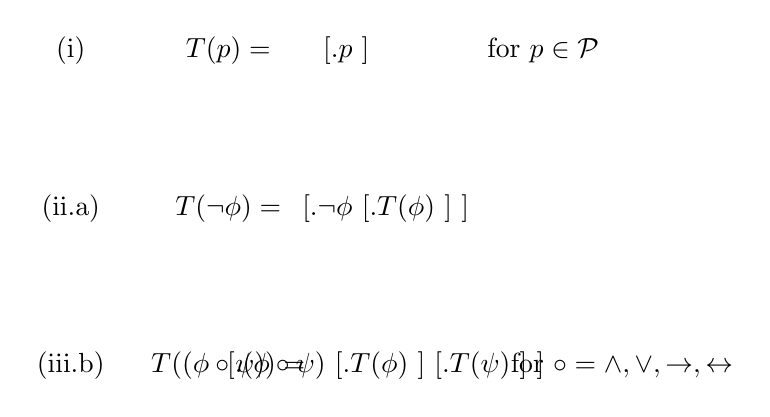
\begin{tikzpicture}
\node at (-2,1) {(i)};

\node at (0,1) {$T(p)=$};
\node at (1.5,1) {\Tree [.$p$ ]};
\node at (4,1) {for $p\in\mathcal{P}$};

\node at (-2,-1) {(ii.a)};
\node at (0,-1) {$T(\neg \phi)=$};
\node at (2,-1) {\Tree [.$\neg \phi$ [.$T(\phi)$ ] ]};

\node at (-2,-3) {(iii.b)};
\node at (0,-3) {$T((\phi\circ\psi))=$};
\node at (2,-3) {\Tree [.$(\phi\circ\psi)$ [.$T(\phi)$ ] [.$T(\psi)$ ] ]};
\node at (5,-3) {for $\circ=\land,\lor,\to,\leftrightarrow$};
\end{tikzpicture}
\end{center}

	What a parsing tree does is, essentially, tell us how the formula in question was constructed. To see how, it's best to look at some examples.
	
	\item One useful piece of terminology: the first sentential operator who's rule is applied when we construct the parsing tree for a formula is called the \emph{main} operator of that formula. This operator will become particularly important when we do semantics in the next chapter. For now, it will allow us to refer to statements based on their main operator:
		\begin{center}
			\begin{tabular}{c | c}
			Main operator & Kind of statement\\\hline
			$\neg$ & a negation\\
			$\land$ & a conjunction\\
			$\lor$ & a disjunction\\
			$\to$ & a conditional\\
			$\leftrightarrow$ & a biconditional
			\end{tabular}
		\end{center}
	
	\item \emph{Examples}. Here are some examples of parsing trees:
			
		\begin{enumerate}[(i)]
		
		\item \
			\begin{center}
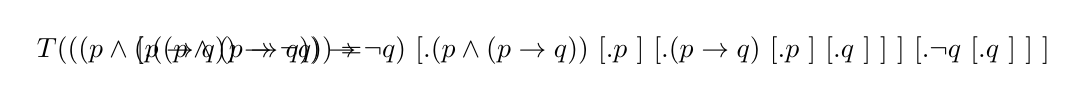
\begin{tikzpicture}
\node at (0,0) {$T(((p\land (p\to q)) \to \neg q))=$};
\node at (5,0) {\Tree [.$((p\land (p\to q))\to \neg q)$ [.$(p\land (p\to q))$ [.$p$ ] [.$(p\to q)$ [.$p$ ] [.$q$ ] ] ] [.$\neg q$ [.$q$ ] ] ]};

\end{tikzpicture}

Main operator: $\to$
\end{center}

		\item \
		
		\begin{center}
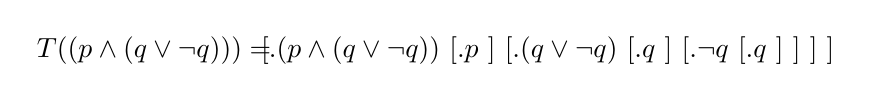
\begin{tikzpicture}
\node at (0,0) {$T((p\land (q\lor \neg q)))=$};
\node at (5,0) {\Tree [.$(p\land (q\lor \neg q))$ [.$p$ ] [.$(q\lor \neg q)$ [.$q$ ] [.$\neg q$ [.$q$ ] ] ] ]};

\end{tikzpicture}

Main operator: $\land$
\end{center}

		\item \
		
		\begin{center}
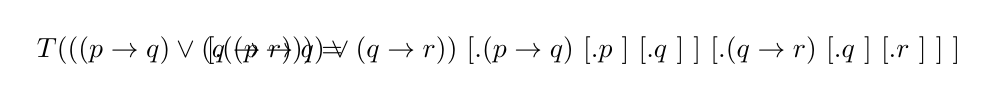
\begin{tikzpicture}
\node at (0,1) {$T(((p\to q)\lor (q\to r)))=$};
\node at (5,1) {\Tree [.$((p\to q)\lor (q\to r))$ [.$(p\to q)$ [.$p$ ] [.$q$ ] ] [.$(q\to r)$ [.$q$ ] [.$r$ ] ] ] };

\end{tikzpicture}

Main operator: $\lor$
\end{center}

			
		\item \
			 
			\begin{center}
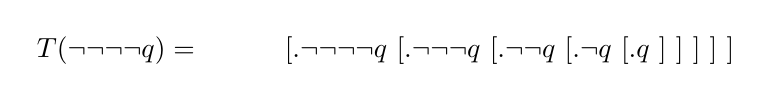
\begin{tikzpicture}
\node at (0,1) {$T(\neg\neg\neg\neg q)=$};
\node at (5,1) {\Tree [.$\neg\neg\neg\neg q$ [.$\neg\neg\neg q$ [.$\neg\neg q$ [.$\neg q$ [.$q$ ] ] ] ] ]};

\end{tikzpicture}

Main operator: $\neg$
\end{center}

In each of these cases, you can read the tree from bottom to top to get a construction of the formula in question from the sentence letters. This is the precise sense in which a parsing tree tracks the construction of a formula.
		
		
		\end{enumerate}
		
	\emph{The following point is the most difficult in this chapter. If you don't get it immediately, don't despair! Follow the advice on reading math: try to think this through, consider examples, draw pictures, etc. And then move on. The details of this proof are not the most important thing to take out of this chapter---the content of the main theorem is!}
		
	\item We will now prove that our recursive definition of $T$ indeed assigns to each formula $\phi$ a unique parsing tree, i.e. we prove that $T$ is a function. We do this in two steps, by proving two central lemmas. In order to properly state these lemmas, we need to read (i) and (ii) from (4.3.5) as \emph{conditions} on something being a tree for a formula---otherwise, we'd already assume the truth of these lemmas. The idea is that, for example, (4.3.5.i) says that a tree $T$ is a parsing tree of $p$ iff $T=p$. And (4.3.5.ii.a) says that $T$ is a parsing tree for $\neg\phi$ iff $T$ is of the form 
	\begin{center}
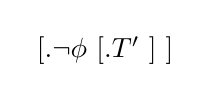
\begin{tikzpicture}
\node at (0,0) {\Tree [.$\neg \phi$ [.$T'$ ] ]};
\end{tikzpicture}
\end{center}
where $T'$ is a parsing tree for $\phi$. Similarly for (4.3.5.ii.b). With this understanding in mind, we can prove the following two lemmas:

		\begin{lemma}[Existence Lemma]
		For each $\phi\in\mathcal{L}$, $T(\phi)$ exists, i.e. there exists a tree that satisfies the conditions (i--ii) from (4.3.5).
		\end{lemma}
		\begin{proof}
		We prove the claim using induction.
		
			\begin{enumerate}[(i)]
			
				\item \emph{Base case}. Let $p\in\mathcal{P}$ be a sentence letter. By (4.3.5.i), $T(p)=p$. And, indeed, $p$ is a tree with $p$ as its only node. Hence, the base case holds.
				
				\item \emph{Induction steps}.
				
					\begin{enumerate}[(a)]
					
						\item Suppose the induction hypothesis that $T(\phi)$ exists. We need to show that $T(\neg \phi)$ exists. By (4.3.5.ii.a), we have that: 
						
						\begin{center}
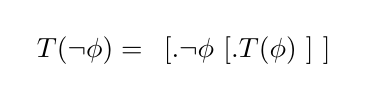
\begin{tikzpicture}
\node at (0,1) {$T(\neg \phi)=$};
\node at (2,1) {\Tree [.$\neg \phi$ [.$T(\phi)$ ] ]};
\end{tikzpicture}
\end{center}
But by the induction hypothesis $T(\phi)$ exists. But if $T(\phi)$ is a tree, so is $T(\neg\phi)$.

				\item Suppose the induction hypotheses that $T(\phi)$ and $T(\psi)$ exist. We need to show that $T((\phi\circ\psi))$ exists for $\circ=\land,\lor,\to,\leftrightarrow$. By (4.3.5.ii.b), we have that: 
						
						\begin{center}
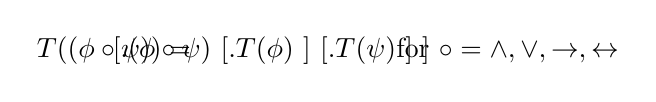
\begin{tikzpicture}
\node at (0,1) {$T((\phi\circ\psi))=$};
\node at (2,1) {\Tree [.$(\phi\circ\psi)$ [.$T(\phi)$ ] [.$T(\psi)$ ] ]};
\node at (5,1) {for $\circ=\land,\lor,\to,\leftrightarrow$};
\end{tikzpicture}
\end{center}
But by the induction hypothesis $T(\phi)$ and $T(\psi)$ both exist. But if $T(\phi)$ is a tree and $T(\psi)$ is a tree, so is $T((\phi\circ\psi))$.					
					\end{enumerate}
			
			\end{enumerate}
			
		Using induction on formulas, we conclude that for each $\phi\in\mathcal{L}$, $T(\phi)$ exists.
		\end{proof}
	\begin{lemma}[Uniqueness Lemma]
	Let $\phi\in\mathcal{L}$. Then $T(\phi)$ is unique, i.e. if $T_1(\phi)$ and $T_2(\phi)$ are two trees that satisfy the conditions (i--ii) from (4.3.5), then $T_1(\phi)=T_2(\phi)$.
	\end{lemma}
	
	\begin{proof}
	We prove this, once more, using induction.
		
			\begin{enumerate}[(i)]
			
				\item \emph{Base case}. Let $p\in\mathcal{P}$ be a sentence letter, and $T_1(p)$ and $T_2(p)$ two trees satisfying the  conditions (i--ii) from (4.3.5). But condition (4.3.5.i) says that $T(p)=p$, so $T_1(p)=p=T_2(p)$, which is what we needed to show.
								
				\item \emph{Induction steps}.
				
					\begin{enumerate}[(a)]
					
					\item Suppose the induction hypothesis that if $T_1(\phi)$ and $T_2(\phi)$ are two trees for $\phi$ which satisfy  conditions (i--ii) from (4.3.5), then $T_1(\phi)=T_2(\phi)$. Now consider two trees for $\neg \phi$, i.e. $T_1(\neg\phi)$ and $T_2(\neg \phi)$. By (4.3.5.ii.a), we have that:	
			\begin{center}
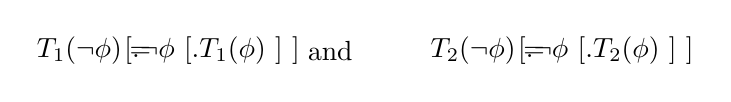
\begin{tikzpicture}
\node at (0,1) {$T_1(\neg \phi)=$};
\node at (1.5,1) {\Tree [.$\neg \phi$ [.$T_1(\phi)$ ] ]};
\node at (3,1) { and};
\node at (5,1) {$T_2(\neg \phi)=$};
\node at (6.5,1) {\Tree [.$\neg \phi$ [.$T_2(\phi)$ ] ]};
\end{tikzpicture}
\end{center}
where $T_1(\phi)$ and $T_2(\phi)$ are trees for $\phi$ which satisfy the conditions  (i--ii) from (4.3.5). But then, by the induction hypothesis, $T_1(\phi)=T_2(\phi)$. And so, $T_1(\neg\phi)=T_2(\neg \phi),$ as desired.

					
						\item Suppose the first induction hypothesis that if $T_1(\phi)$ and $T_2(\phi)$ are two trees for $\phi$ which satisfy  conditions (i--ii) from (4.3.5), then $T_1(\phi)=T_2(\phi)$. And suppose further that if $T_1(\psi)$ and $T_2(\psi)$ are two trees for $\psi$ which satisfy  conditions (i--ii) from (4.3.5), then $T_1(\psi)=T_2(\psi)$.
						
						Now consider two trees for $(\phi\circ\psi)$, for $\circ=\land,\lor,\to,\leftrightarrow$, $T_1((\phi\circ\psi))$ and $T_2((\phi\circ\psi))$. By (4.3.5.ii.a), we have that:	
			\begin{center}
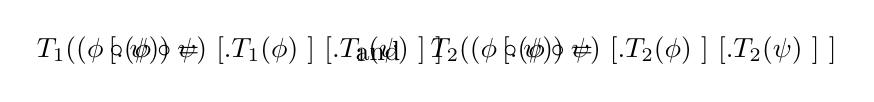
\begin{tikzpicture}
\node at (0,1) {$T_1((\phi\circ\psi))=$};
\node at (2,1) {\Tree [.$(\phi\circ\psi)$ [.$T_1(\phi)$ ] [.$T_1(\psi)$ ] ]};
\node at (3.3,1) { and};
\node at (5,1) {$T_2((\phi\circ\psi))=$};
\node at (7,1) {\Tree [.$(\phi\circ\psi)$ [.$T_2(\phi)$ ] [.$T_2(\psi)$ ] ]};
\end{tikzpicture}
\end{center}
where $T_1(\phi)$ and $T_2(\phi)$ are trees for $\phi$ which satisfy the conditions  (i--ii) from (4.3.5), and $T_1(\psi)$ and $T_2(\psi)$ are trees for $\psi$ which satisfy the conditions  (i--ii) from (4.3.5). But then, by the induction hypotheses, $T_1(\phi)=T_2(\phi)$ and $T_1(\psi)=T_2(\psi)$. And so, $T_1((\phi\circ\psi))=T_2((\phi\circ\psi)),$ as desired.

	\end{enumerate}
	
	\end{enumerate}
	
We conclude by using (i) and (ii) to infer by induction that the parsing tree for every formula is unique.
	
\end{proof}
	
	Put together, the two lemmas yield our unique readability theorem:
	\begin{theorem}
	For each formula $\phi\in\mathcal{L}$ there exists a unique parsing tree, $T(\phi)$ as defined by (4.3.5).
	\end{theorem}
	
	This theorem is of fundamental importance for what we're doing in propositional logic. Essentially, it guarantees that we can use function recursion on $\mathcal{L}$. Why? Because the theorem tells us that we can calculate a recursively defined function on $\mathcal{L}$ following the formulas parsing tree---\emph{and this is the only way in which the function can be calculated}. In fact, this theorem guarantees that propositional logic can be computer implemented---a computer can construct the parsing tree for a formula in order to ``understand'' it.
	
	\item We'll conclude the section by discussing an \emph{algorithm} for determining whether a given expression $\sigma$ is a formula. First, let's clarify what we understand under the term ``algorithm.'' In mathematics, an algorithm is typically understood as a finite set of precise instructions which, if followed, are supposed to complete a specific task. Hence an algorithm itself is not a computer program but the procedure that underlies the computer program. We can thus describe an algorithm in natural language without focusing on a specific \emph{implementation} of the algorithm in a programming language. 
	
	\item The task that our algorithm is supposed to fulfill is to determine whether a given expression is a formula. We hereby assume that the expression is formed entirely out of symbols from the alphabet, since by 4.2.5, if it's not, we can already exclude that it's a formula. Here is our algorithm:
	\begin{enumerate}[1.]
			
				\item Write down the expression $\sigma$ and look at it. Proceed to step 2.
				
				\item Does the expression you're currently looking at contain the same number of $($'s and $)$'s?
				\begin{enumerate}[(a)]
				
					\item If not, terminate: $\sigma$ is not a formula!
					
					\item If yes, proceed to step 3.
				
				\end{enumerate}
				
				\item Is the expression you're currently looking at of the form $p$?
				
				\begin{enumerate}[(a)]
				
					\item If not, proceed to step 4.
				
					\item If yes, write a $\checkmark$ next to it and proceed to step 6.
					
				\end{enumerate}
				
				\item Is the expression you're currently looking at of the form $\neg \tau$?

				\begin{enumerate}[(a)]
				
					\item If not, proceed to step 5.

					
					\item If yes, apply the following rule:
					\begin{center}
					\Tree [.$\neg \tau\checkmark$ [.$\tau$ ] ]
					\end{center}
					Then proceed to step 6.
										
				
				\end{enumerate}
											
	
			\item Is the expression you're currently looking at of the form $(\tau\circ\pi)$, $\circ=\land,\lor,\to,\leftrightarrow$,  and there is no other connective $\square=\land,\lor,\to,\leftrightarrow$ such that the expression is of the form $(\tau'\square\pi')$ and $\square$ is enclosed in fewer parentheses than $\circ$?				
	
			\begin{enumerate}[(a)]
		
				\item If not, terminate: $\sigma$ is not a formula!
				
				\item If yes, apply the following rule:
			
				\begin{center}
				\Tree [.$(\tau\circ\pi)\checkmark$ [.$\tau$ ] [.$\pi$ ] ]
				\end{center}
			
				Then proceed to step 6.	
			
			\end{enumerate}
		
			\item In the tree you've constructed so far, is there an expression at a leaf without a $\checkmark$ next to it?
		
			\begin{enumerate}[(a)]
			
				\item If no, terminate: $\sigma$ is a formula \smiley		
				
				\item If yes, then pick one and look at it. Go back to step 2.
			
		
			\end{enumerate}
	
		\end{enumerate}
		
	\item We will not prove that this algorithm actually completes its task, we won't \emph{formally verify} the algorithm. To do so, is actually not that hard given all the facts we've already observed. But it's tedious and so we'll leave the task to the interested reader. Note that what you would need to show are three things: (i) the algorithm always terminates, (ii) if the algorithm terminates and says that the expression is a formula, then it is indeed a formula, and (iii) if the algorithm terminates and says that the expression is not a formula, then it is indeed not a formula. Here we simply observe (again without proof) that the algorithm, if applied to a formula, actually yields the parsing tree of that formula. To see this, try it out! Apply the algorithm to some formulas and see what you get. Here we give just one example:
	\begin{center}
	\Tree[.$(p\lor (q\lor (r\leftrightarrow (\neg s\land t))))\checkmark^{5.b}$ [.{$p\checkmark^{3.b}$} ] [.{$(q\lor (r\leftrightarrow (\neg s\land t)))\checkmark^{5.b}$} [.{$q\checkmark^{3.b}$} ] [.{$(r\leftrightarrow (\neg s\land t))\checkmark^{5.b}$} [.$r\checkmark^{3.b}$ ] [.$(\neg s\land t)\checkmark^{5.b}$ [.$\neg s\checkmark^{4.b}$ [.$s\checkmark^{3.b}$ ] ] [.$t\checkmark^{3.b}$ ] ] ] ] ]
	
	\emph{Note that in the first step (5.b), we parse according to the first $\lor$ because it's in fewer parentheses than the second $\lor$, the $\leftrightarrow$ and the $\land$.}
	\end{center}
	So, effectively, what the algorithm does is what a computer would do (described on a very abstract level) if given an expression and asked whether it makes sense in propositional logic.
	
	\item We conclude the section with two example applications of the algorithm to illustrate how it can be used to show that something \emph{isn't} a formula:
	
		\begin{enumerate}[(i)]
		
			\item \emph{Claim}. $((p\land q)\to (r))\notin\mathcal{L}$
			
			\item[] \emph{Algorithmic proof}.

			\begin{center}		
				\Tree [.$((p\land q)\to \neg(r))\checkmark^{5.b}$ [.$(p\land q)\checkmark^{5.b}$ [.$p\checkmark^{3.b}$ ] [.$q\checkmark^{3.b}$ ] ] [.$\neg(r)\checkmark^{4.b}$ [.$(r)\frownie^{5.a}$ ] ] ] 
			\end{center}
			
			\item \emph{Claim}. $\neg\neg(p(\leftrightarrow) q)\notin\mathcal{L}$.
			
			\item[] \emph{Algorithmic proof}.
			
				\begin{center}
				\Tree [.${\neg\neg(p(\leftrightarrow) q)}\checkmark^{4.b}$ [.${\neg(p(\leftrightarrow) q)}\checkmark^{4.b}$ [.${(p(\leftrightarrow) q)}\checkmark^{5.b}$ [.$(p(\frownie^{2.a}$ ] [.$)q)\frownie^{2.a}$ ] ] ] ]
				\end{center}
		\end{enumerate}
	
	\end{enumerate}
	
	
\section{Function Recursion on Propositional Languages}

	\begin{enumerate}[\thesection.1]

		\item In the previous section, we've given a justification for using function recursion on $\mathcal{L}$. Now, we'll define two important syntactic functions, i.e. functions with domain $\mathcal{L}$. The importance of these functions derives from their wide-spread use in logical literature (way beyond propositional logic). But also in our course, they will play an important role here and there.
		
	  \item The first of the two functions, we'll define a function that maps each formula to the set of formulas it was constructed from.
		These formulas are called the \emph{sub-formulas} of the formula in question.
		We define the function as follows using function recursion:
		\begin{enumerate}[(i)]
		  \item%
			$sub(p)=\{p\}$ for $p\in\mathcal{P}$
		  \item%
			\begin{enumerate}[(a)]
			  \item%
				$sub(\neg\phi)= sub(\phi)\cup\{\neg \phi\}$
			  \item%
				$sub((\phi\circ\psi))= sub(\phi)\cup sub(\psi)\cup\{(\phi\circ\psi)\}$
			\end{enumerate}
		\end{enumerate}
		Let's consider two examples.
		We have:
		\begin{itemize}
		  \item%
			$sub(\neg \neg p)=\{p,\neg p, \neg\neg p\}$
		  \item%
			$sub(((p\land q)\lor r))=\{p,q,r,(p\land q), ((p\land q)\lor r)\}$
		\end{itemize}
		In order to understand this definition,
		follow the advice for understanding a definition from lecture 2!

	\item One thing that might help us understanding sub-formulas better is to compare them to notions we've previously introduced. For this purpose, we'll prove the following proposition:
	
		\begin{proposition}
		Let $\phi\in\mathcal{L}$ be a formula. Then the elements of $sub(\phi)$ are precisely the formulas that occur in $T(\phi)$.
		\end{proposition}
		\begin{proof}
		We prove this fact using---surprise---induction.
		
		\begin{enumerate}[(i)]
		
			\item \emph{Base case}. Let $p\in\mathcal{P}$ be a sentence letter. Then $sub(p)=\{p\}$ and $T(p)=p$. Hence $sub(p)$ is precisely the set of formulas that occur in $T(p)$.
			
			\item \emph{Induction steps}. 
				\begin{enumerate}[(a)]

					\item Assume the induction hypothesis that $sub(\phi)$ are precisely the formulas that occur in $T(\phi)$. Now consider $\neg \phi$. We know by definition of $sub$, that $sub(\neg\phi)=sub(\phi)\cup\{\neg\phi\}$. By the (ii.a) definition of parsing trees, we know furthermore that:
					\begin{center}
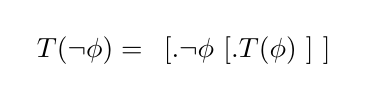
\begin{tikzpicture}
\node at (0,0) {$T(\neg \phi)=$};
\node at (2,0) {\Tree [.$\neg \phi$ [.$T(\phi)$ ] ]};
\end{tikzpicture}
\end{center}
Hence the formulas that occur in $T(\neg\phi)$ are precisely the formulas that occur in $T(\phi)$ plus the formula $\neg\phi$. But this is just another way of saying that the formulas in $T(\neg\phi)$ are  $sub(\phi)\cup\{\neg\phi\}=sub(\neg\phi),$ as desired.

			\item Assume the induction hypotheses that $sub(\phi)$ are precisely the formulas that occur in $T(\phi)$ and $sub(\psi)$ are precisely the formulas ocuring in $T(\psi)$. Now consider $(\phi\circ\psi)$, for $\circ=\land,\lor,\to,\leftrightarrow$. We know by definition of $sub$, that $sub((\phi\circ\psi))=sub(\phi)\cup sub(\psi)\cup\{(\phi\circ\psi)\}$. By the (ii.a) definition of parsing trees, we know furthermore that:
					\begin{center}
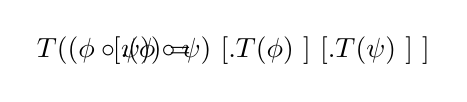
\begin{tikzpicture}
\node at (0,0) {$T((\phi\circ\psi))=$};
\node at (2,0) {\Tree [.$(\phi\circ\psi)$ [.$T(\phi)$ ] [.$T(\psi)$ ] ]};
\end{tikzpicture}
\end{center}
Hence the formulas that occur in $T((\phi\circ\psi))$ are precisely the formulas that occur in $T(\phi)$, plus the formulas in $T(\psi)$, plus $(\phi\circ\psi)$. But this is just another way of saying that the formulas in $T((\phi\circ\psi))$ are $sub(\phi)\cup sub(\psi)\cup\{(\phi\circ\psi)\}=sub((\phi\circ\psi)),$ as desiderd.

				\end{enumerate}
		
		\end{enumerate}
		We can thus use induction to infer that the claim holds for all $\phi$.		
		\end{proof}

	\item We move to the second important syntactic function, the so-called measure of \emph{complexity}. In order to define this function, we make use of the maximum function $max:\mathbb{N}^2\to\mathbb{N}$, which is defined as follows:
	\[max(n,m)=\begin{cases} n &\text{if }n>m\\ m &\text{if }m>n\\n& \text{if }n=m\end{cases}\] So, we get, for example, $max(2,3)=3, max(3,2)=3, max(2,2)=2$, and so on. Using $max$, the (recursive) definition of the complexity function $c:\mathcal{L}\to\mathbb{N}$ is as follows:
	\begin{enumerate}[(i)]
	
		\item $c(p)=0$ for $p\in\mathcal{P}$
		
		\item \begin{enumerate}[(a)]
		
			\item $c(\neg\phi)=c(\phi)+1$
			
			\item $c((\phi\circ\psi))=max(c(\phi), c(\psi))+1$, for $\circ=\land,\lor,\to,\leftrightarrow$.
		
		\end{enumerate}
	
	\end{enumerate}
Let's consider some examples. We have:
	\begin{itemize}
	
		\item $c(\neg p)=1$, $c((p\land q))=1, c((p\lor q)=1, \mathellipsis$
		
		\item $c(\neg\neg p)=2$, $c(\neg (p\land q))=2$, $c((\neg p\land \neg q))=2, \mathellipsis$
	
	\end{itemize}
	
	Can we somehow narrow down what $c$ precisely measures? Think about it before you read the next point. 

	\item We will now prove a proposition that gives us an intuitive reading of the function $c$:
	
	\begin{proposition}
	Let $\phi\in\mathcal{L}$ be a formula. Then $c(\phi)$ is the length of the longest path in $T(\phi)$ which starts from the root (counted in number of edges travelled). In other words, $c(\phi)$ gives us the \emph{height} of the parsing tree $T(\phi)$.
	\end{proposition}
	\begin{proof}
	How are we going to prove this? You know it!
	
\begin{enumerate}[(i)]
		
			\item \emph{Base case}. Let $p\in\mathcal{P}$ be a sentence letter. Then $T(p)=p$. But the only path you can travel from the root in $p$ is the trivial path of length zero, which just stops immediately at $p$. Since $c(p)=0$, this just means that the base case holds.
			
			\item \emph{Induction steps}. 
				\begin{enumerate}[(a)]

					\item Assume the induction hypothesis that $c(\phi)$ is the length of the longest path from the root in $T(\phi)$. Now consider $\neg \phi$. By the (ii.a) definition of parsing trees, we know that:
					\begin{center}
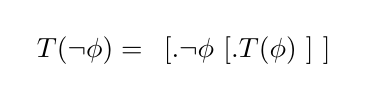
\begin{tikzpicture}
\node at (0,0) {$T(\neg \phi)=$};
\node at (2,0) {\Tree [.$\neg \phi$ [.$T(\phi)$ ] ]};
\end{tikzpicture}
\end{center}
Now think about the longest path you can travel from the root in $T(\neg\phi)$. Well, it's going to be the longest path you can travel in $T(\phi)$ plus one edge to the new root, i.e. $\neg\phi$. Since $c(\neg\phi)=c(\phi)+1$, this means that, by the induction hypothesis, the claim holds.

			\item Assume the induction hypotheses that $c(\phi)$ is the length of the longest path from the root in $T(\phi)$ and $c(\psi)$ is the length of the longest path from the root in $T(\psi)$. By the (ii.a) definition of parsing trees, we know that:
					\begin{center}
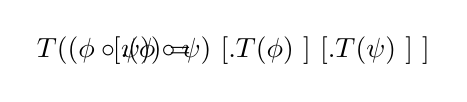
\begin{tikzpicture}
\node at (0,0) {$T((\phi\circ\psi))=$};
\node at (2,0) {\Tree [.$(\phi\circ\psi)$ [.$T(\phi)$ ] [.$T(\psi)$ ] ]};
\end{tikzpicture}
\end{center}
Now think about the longest path you can travel in $T((\phi\circ\psi))$. Well, take the longest path you can find in either $T(\phi)$ or $T(\psi)$. Let's suppose that the path is in $T(\phi)$ (if it is in $T(\psi)$, the argument is completely analogous). The longest path you can travel from the root in $T((\phi\circ\psi))$ is going to be precisely this path plus the one new edge connecting $T(\phi)$ to the new root $(\phi\circ\psi)$. Since $c((\phi\circ\psi))=max(c(\phi),c(\psi))+1$, this just means that the claim also holds here. 
				\end{enumerate}
		
		\end{enumerate}
		We can thus use induction to infer that the claim holds for all $\phi$.			
	\end{proof}
	
	\item This completes our discussion of function recursion on $\mathcal{L}$ by means examples. In order to get a real good grip on how the method works, it's best for you to try your hand at it, i.e. try to define your own syntactic functions using function recursion. Among the exercises, you can find some functions you can try to define.

	\end{enumerate}

\section{Some Useful Notational Conventions}

	\begin{enumerate}[\thesection.1]

		\item So far, we've been very precise about our use of parentheses. And for good reason: as we discussed in \S4.3, our tidy use of parentheses is what guaranteed unique readability. But, at the same time, writing all of these parentheses can be exhausting. And, as I said in the lecture, logicians are lazy: they don't like to do unnecessary things. So, over the years, some generally agreed upon conventions have emerged for leaving out parentheses, which we'll briefly discuss in this section.
		
		\item Before we begin, note that conventional notation is only ever allowed outside the context of syntax theory, i.e. in semantics and proof theory. And even there, it's often better to be safe than sorry. As we said a couple of times by now: the parentheses are there for a reason. It's much easier to make mistakes using conventional notation than it is in official notation. That being said, conventional notation can be a real boon on your wrist.
		
		\item The first convention is that you can always omit any outermost parentheses. So, instead of $(p\land q)$, you can simply write $p\land q$. The reasoning behind this is that these are easy to fill in: if a logician writes $p\lor q$, it's pretty clear what they mean: $(p\lor q$).
		
		\item The second convention is that in a series of $\lor$'s or $\land$'s, you can leave out the repeatedly nested parentheses. So, for example, instead of the official $((p\land (q\land (r\land (s\land t)))))$, we can simply write $p\land q\land r\land s\land t$ (also applying the convention about outermost parentheses). Note that this convention really introduces some ambiguity into our language. The conventional formula $p\lor q\lor r$ has indeed two ways of being parsed:
		\begin{center}
		
		\begin{tabular}{c c c}
		\begin{tikzpicture}
		{\Tree [.$p\lor q\lor r$ [.$p$ ] [.$q\lor r$ [.$q$ ] [.$r$ ] ] ]}
		\end{tikzpicture}

		& 
		
		\qquad \raisebox{7.5ex}{vs.} \qquad 
				\begin{tikzpicture}

		{\Tree [.$p\lor q\lor r$ [.$p\lor q$ [.$p$ ] [.$q$ ] ] [.$r$ ] ]}
		\end{tikzpicture}

		\end{tabular}
		\end{center}
This makes the convention a bit harder to justify. But note that the two different ``readings'' of the formula don't really say anything different. Take the following two sentences: 
	\begin{itemize}

		\item I have toast, or I have eggs or pancakes
		
		\item I have toast or eggs, or I have pancakes

	\end{itemize}
They really seem to say the same thing. We'll only be able to properly justify the convention in the next chapter, when we talk about logical equivalence, but for now, I hope these examples illustrate why we can allow for this little bit of ambiguity. Note that in \emph{mixed} series of $\land$ and $\lor$, we \emph{cannot} omit parentheses. I.e. $p\land (q\lor r)$ needs to stay just that.

		\item Finally, the most complicated convention concerns the interaction of the connectives. The idea is that if we agree upon which connective we should read first, we can drop a bunch of parentheses. For example, if we say that we always read $\to$ before $\land$ if there's an ambiguity, then the previously ambiguous expression $p\land q\to r$, with the two readings
				\begin{center}
		
		\begin{tabular}{c c c}
		\begin{tikzpicture}
		{\Tree [.$p\land q\to r$ [.$p$ ] [.$q\to r$ [.$q$ ] [.$r$ ] ] ]}
		\end{tikzpicture}

		& 
		
		\qquad \raisebox{7.5ex}{vs.} \qquad 
				\begin{tikzpicture}

		{\Tree [.$p\land q\to r$ [.$p\land q$ [.$p$ ] [.$q$ ] ] [.$r$ ] ]}
		\end{tikzpicture}

		\end{tabular}
		\end{center}
now unambiguously, gets the second of the two readings. That is, $p\land q\to r$ is then simply read as $(p\land q)\to r$. This is the idea of \emph{binding strength}: we say that $\land$ \emph{binds stronger} than $\to$. This idea allows us to leave out a bunch of parentheses, which we can easily fill in by reading the right operator first. 

	\item The relative binding strength of the operators is given in the following diagram:
\[{\neg}>{\land}={\lor}>{\to}>{\leftrightarrow}.\] Explicitly, this means that, in a case of conflict, you always read the $\leftrightarrow$ first, then $\to$, then $\lor$ and $\land$, and only finally $\neg$. Note that $\land$ and $\lor$ have precisely the same binding strength, so in expressions like $p\land (q\lor r)$, we really can't leave out any parentheses. But if we consider an expression like $((p\land q)\leftrightarrow (p\leftrightarrow q))$, we can easily leave out a some:
	\begin{itemize}
	
		\item According to the first convention, we can leave out the outermost parentheses, yielding $(p\land q)\leftrightarrow (p\leftrightarrow q)$.
		
		\item Now, since we know that we'll always parse according to $\leftrightarrow$ before $\land$, this means that we can leave out the parentheses around the $\land$, giving us $p\land q\leftrightarrow (p\leftrightarrow q)$.
		
		\item Can we also leave out the last pair of parentheses? ---No! For in $p\land q\leftrightarrow p\leftrightarrow q$, there would be a conflict between two readings:
	\begin{center}
		
		\begin{tabular}{c c c}
		\begin{tikzpicture}
		{\Tree [.$p\land q\leftrightarrow p\leftrightarrow q$ [.$p\land q$ [.$p$ ] [.$q$ ] ] [.$p\leftrightarrow q$ [.$p$ ] [.$q$ ] ] ]}
		\end{tikzpicture}

		& 
		
		\qquad \raisebox{7.5ex}{vs.} \qquad & 
				\begin{tikzpicture}
		{\Tree [.$p\land q\leftrightarrow p\leftrightarrow q$ [.$p\land q\leftrightarrow p$ [.$p\land q$ [.$p$ ] [.$q$ ] ] [.$p$ ] ] [.$q$ ] ]}
		\end{tikzpicture}

		\end{tabular}
		\end{center}
		
		\item So, the best we can do is $p\land q\leftrightarrow (p\leftrightarrow q)$.
	
	\end{itemize}
	
	\item These ideas need some getting used to. For that reason, there are plenty of exercises included at the end of this section (4.8.9 and 4.8.10), solutions for which can be found in the appendix.
	
	\item We conclude with a last remark about conventional notation. You might wonder: Well, these are pretty clear conventions. Surely, a computer can learn them. Why can't we devise an official definition that has unique readability and respects these conventions? ---And you would be right! This \emph{is} possible. It's just not very practical for most purposes. The official definition of a formula would thereby become much more complicated. This would have the consequence that proofs by induction and function recursion would become horribly complicated to carry out, too. Additionally, if we care about efficiency (as we often do with computers), it turns out to be way more efficient to use our official definition and to translate between official and conventional notation that to carry out everything in conventional notation. And you can essentially see why: because \emph{every} recursive definition would become more complicated---and we need \emph{a lot} of them. So, we'll stick to our official notation for official purposes and use conventional notation for fun. 

	\end{enumerate}

\section{Core Ideas}

\begin{itemize}

	\item A formal language is defined by a vocabulary (symbols) and a grammar (rules for well-formed expressions).
	
	\item The vocabulary of a propositional language consists of a set of sentence letters $\mathcal{P}$, the sentential connectives $\neg,\land,\lor,\to,\leftrightarrow$, and the parentheses $($ and $)$.
	
	\item The set $\mathcal{L}$ of formulas is inductively defined as the smallest set containing the sentence letters and which is closed under the sentential connectives. 
	
	\item Formalization is the process of abstracting ordinary language expressions into a propositional language. \emph{Use the guidelines}.
	
	\item Syntactic recursion works by specifying the value for the sentence letters and how to calculate the value for a complex formula from the values for its subformulas.
	
	\item The parsing tree of a formula gives you its internal structure: it shows how the formula was constructed.
	
	\item The unique readability theorem guarantees that syntactic recursion works and that formulas are computer readable. It states that every formula has a unique parsing tree.
	
	\item There is a useful algorithm for checking whether an expression is a formula.
	
	\item Outside of syntax theory, the notational conventions are useful. But use them with caution.

\end{itemize}

\section{Self Study Questions}

	\begin{enumerate}[\thesection.1]

		\item Suppose that an expression contains absolutely no parentheses. What is the best we can say about the expression?
		
			\begin{enumerate}[(a)]

				\item The expression is not a formula.
				
				\item If the expression is a formula, then it is a sentence letter.
				
				\item If the expression is a formula, then it cannot contain $\land,\lor,\to,\leftrightarrow$.
				
				\item There is an even number of negations in the expression.
	
			\end{enumerate}
			
		\item You're asked to determine whether an expression is a formula. In which order would you apply the following techniques?
		
		\begin{enumerate}[(a)]
		
			\item Try to prove it definitionally (as in 4.1.9)
		
			\item Check whether the expression contains symbols not from the vocabulary (using Proposition 4.2.5).
			
			\item Apply the algorithm (4.3.10).
			
			\item Check whether the expression contains as many $($'s as $)$'s (using the solution to exercise (4.8.8).
		
		\end{enumerate}
		
	\item Can you always see whether a formula is written in conventional notation?
	
	\begin{enumerate}[(a)]
	
		\item Yes, I simply construct the parsing tree for the expression.
		
		\item No, because a formula written in notational convention does  not need to contain an even number of parentheses.
	
		\item Yes, you can apply the algorithm (4.3.10) for that.
	
		\item No, it needs to be clear from the context.
	
	\end{enumerate}
	
	\item A formula has complexity four. Which of the following can you infer from that?
		
		\begin{enumerate}[(a)]
		
			\item The formula contains at least four connectives.
			
			\item The formulas contains at most four connectives.
			
			\item The formula contains at most four negations.
			
			\item The parsing tree of the formula has at most four nodes.

			\item The parsing tree of the formula has exactly four nodes.
			
			\item The parsing tree of the formula has at least five nodes.
		
		\end{enumerate}

	\end{enumerate}
\section{Exercises}


	\begin{enumerate}[\thesection.1]
	
		\item $[h]$ Translate the following statements into a suitable propositional language! Don't forget the translation key.
			
			\begin{enumerate}

				\item Alan Turing built the first computer but Ada Lovelace invented the first computer algorithm.
			
				\item Only if Alan Turing built the first computer, it's Monday today.
			
				\item Either Alan Turing or Ada Lovelace is your favorite computer scientist.
			
				\item Today is Monday if and only if both yesterday was Tuesday and tomorrow is Saturday.
			
			\end{enumerate}

		\item $[h]$ Translate the following statements into English/Dutch. Use the following translation key: 
		
		\begin{center}
			\begin{tabular}{c c l}
		
			 $p$ & : & I'm happy/Ik ben blij\\[1ex]
			
			 $q$ & : & I clap my hands/Ik klap in mijn handen\\[1ex]
			
			 $r$ & : & You're happy/Jij bent blij\\[1ex]
			
			 $s$ & : & You clap your hands/Jij klapt in je handen\\[1ex]
			
			 $t$ & : & We both clap our hands/Wij klappen in onze handen
			 \end{tabular}
		
		\end{center}
		
		\begin{enumerate}[(a)]
		
			\item $\neg\neg (p\land q)$
		
			\item $(\neg p\to \neg q)$
			
			\item $(p\leftrightarrow (\neg r\land q))$
			
			\item $((q\land s)\to t)$
		
			\item $((q\land s)\to (p\lor r))$
			
			\item $(((p\land q)\lor (r\land s))\land \neg ((p\land q\land r\land s)))$
		
		\end{enumerate}
		
		\item Give an inductive definition of the set of all formulas of $\mathcal{L}$ that only contain $p,q,\neg,\land,(,$ and $)$.
		
		\item Use the algorithm from 4.3.10 to decide whether the following expressions are formulas:
		
		\begin{enumerate}[(a)]
		
			\item $(q\leftrightarrow (p\land (q\lor (r\land \neg s)))$
		
			
			\item $((p\land q)\lor (p\land (q\to\neg q)))$
			
			\item $(p\to (p\to ((p\land p)\leftrightarrow p\lor p)))$
			
			\item $\neg\neg (\neg\neg p\land (q\lor q) )$
			
		\end{enumerate}
		
		\item Use function recursion to define the following syntactic functions:
		
		\begin{enumerate}
		
			\item $[h]$ the function $\#_{conn}:\mathcal{L}\to\mathbb{N}$, which counts the number of sentential connectives in a formula $\phi$.
			
			\item the function $\#_(:\mathcal{L}\to\mathbb{N}$, which counts the number of left brackets in a formula $\phi$. 
			
			\item the function $\#_{\mathcal{P}}:\mathcal{L}\to\mathbb{N}$, which counts the number of sentence letters in a formula $\phi$.
			
			\item the function $\mathbf{1}_p:\mathcal{L}\to\{0,1\}$, which assigns one to a formula $\phi$ if $p\in sub(\phi)$ and zero otherwise.
		
		\end{enumerate}
		
		\item $[\nosym]$ Consider the following recursively defined functions on $\mathcal{L}$. What do they (in ordinary words) measure?
		
			\begin{enumerate}[(a)]
			
				\item $f:\mathcal{L}\to\mathbb{N}$ defined by:
				
					\begin{enumerate}[(i)]

					\item $f(p)=1,$ for $p\in\mathcal{P}$

					\item 			\begin{enumerate}[(a)]

					\item $f(\neg \phi)=f(\phi)+1,$

					\item $f((\phi\circ \psi))=f(\phi)+f(\psi)+3,$ for $\circ=\land,\lor,\to,\leftrightarrow.$
					
					\end{enumerate}
					\end{enumerate}
					
				\item $g:\mathcal{L}\to\mathbb{N}$ defined by:
				
					\begin{enumerate}[(i)]

					\item $g(p)=0,$ for $p\in\mathcal{P}$

					\item 			\begin{enumerate}[(a)]

					\item $g(\neg \phi)=g(\phi)+1,$

					\item $g((\phi\circ \psi))=g(\phi)+g(\psi),$ for $\circ=\land,\lor,\to,\leftrightarrow.$
					
					\end{enumerate}
					\end{enumerate}
					
					\item (this is a tricky one) $h:\mathcal{L}\to\{0,1\}$ defined by:
				
					\begin{enumerate}[(i)]

					\item $h(p)=1,$ for $p\in\mathcal{P}$

					\item 			\begin{enumerate}[(a)]

					\item $h(\neg \phi)=\begin{cases}
					0 &\text{if }h(\phi)=1\\
					1 & \text{if }h(\phi)=0
					\end{cases}$

					\item $h((\phi\circ \psi))=\begin{cases}
					1&\text{if }h(\phi)=1\text{ and }h(\psi)=1\\
					1&\text{if }h(\phi)=0\text{ and }h(\psi)=0\\
					0 & \text{otherwise}
					\end{cases}$ 
					
					\item[] for $\circ=\land,\lor,\to,\leftrightarrow.$
					
					\end{enumerate}
					\end{enumerate}
			
			\end{enumerate} 
		
		\item Use proof by induction to prove that the number of elements in $sub(\phi)$ is at most $2\cdot \#_{conn}(\phi)+1$.

		\item $[h]$ Prove (using induction on formulas) that for each formula $\phi\in\mathcal{L}$, the number of $($'s and the number of $)$'s is equal. Derive as a corollary a necessary condition for formula-hood and discuss why the condition is better than the one given in (4.2.4).
		
		\item Translate the following formulas written using the notational conventions into official notation:
		
		\begin{enumerate}[(a)]

		\item  $\neg p\land q$

		\item  $\neg(p\land q\to \neg p\lor\neg q)$
		
		\item  $p\lor p\leftrightarrow \neg p$

		\item  $(p\lor q)\land r$
		
		\item $p\to p\leftrightarrow p\to p$

		\item  $\neg p \land (q\lor r\to p\leftrightarrow q)$
		
		\item $p\land (p\lor q)$ 

		\item $p\to q\lor q\leftrightarrow r$

		\item $p\to q\leftrightarrow \neg q\to \neg p$  

		\item $\neg\neg\neg p$

		\item ${p} \to {p} \leftrightarrow {p}\lor \neg {p}$

		\item $p\lor q\to \neg r\land (s\leftrightarrow {p})$

		\end{enumerate}
		
	\item Take the following formulas and write them according to our notational conventions:
	
		\begin{enumerate}
		
			\item $(p\land q)$
		
			\item $\neg\neg q$
			
			\item $(p\land (r\lor q))$
			
			\item $(p\to (r\lor (p\land (q\leftrightarrow r))))$
			
			\item $(p\lor \neg (p\lor q))$
			
			\item $((p\land q)\to r)$
			
			\item $(((p\lor q)\to \neg q)\leftrightarrow r)$
			
			\item $((p\land q)\land r)$
			
			\item $(p\land (q\land r))$
			
			\item $(p\lor (q\lor r))$
			
			\item $(p\land (q\lor r))$
			
			\item $(p\land (q\to r))$
				
		\end{enumerate}
		
		\item (This is a real challenge, only try this is you have enough time and energy): Write an algorithm that translates a formula from conventional into official notation. 

	\end{enumerate}

\section{Further Readings}

We're starting to get into logic proper. Recommendations for further readings that I can give you at this point will be chapters from other logic books, which cover the same material but in slightly different way. Note, however, that if you look into another logic textbook, you will (most likely) encounter different ways of doing things. Here are just some examples of what I mean:
	\begin{itemize}
	
		\item Some authors use different terminology. For example, they may call sentence letters ``propositional variables'' or sentential connectives ``propositional connectives.''
		
		\item Some authors may have different definitions of formulas. It's possible, for example, to demand that also negations are enclosed by parentheses, so that $\neg p$ is not a formula only $(\neg p)$ is.
	
		\item Some authors use different symbols for the connectives, such as $\supset$ instead of our $\to$ or $\equiv$ instead of our $\leftrightarrow$. 
		
		\item Some authors use $A,B,C,\mathellipsis$ for formulas, rather than our $\phi,\psi,\theta,\mathellipsis.$
		
		\item Some authors might use proof by induction in a different (but equivalent) way. For example, they might use mathematical induction on the complexity of formulas instead of our method, which is known in the literature as \emph{structural} induction.
		
		\item Some authors may use terminology in a slightly different way. For example, complexity is sometimes defined so that it doesn't correspond to the height of the parsing tree but rather the number of logical connectives in the formula. 
		
		\item They might prove different theorems or the same theorems in different ways.
	
	\end{itemize}
	
These are really just some of the possible differences you may encounter. If you continue with my literature recommendations, you have to brace yourself for that. But there are also some reasons for why it's a good idea to look at other texts despite these potential obstacles:
	\begin{itemize}
	
		\item Regardless of these differences, the books that I'm recommending are dealing with the same subject matter---just in a slightly different way. And this different perspective might help you understand better what's going on.
		
		\item When you continue your studies, you will see that there are  many, many different notations or, more generally, ways of doing things around. This equally applies in logic, mathematics, computer science, and other related disciplines. The earlier you get used to the plurality, the better.
			
		\item Other textbooks are a great source of additional exercises (though typically without solutions, as I mentioned in the lecture).	
			
	\end{itemize}
So, here are my recommendations for book-chapters that deal with the same material in comparable ways. 

	\begin{itemize}
	
		\item Section 2.1 of Dalen, Dirk van. 2013. \emph{Logic and Structure}. 5$^\text{th}$ edition. London, UK: Springer.
		
		\item Sections 1.0, 1.1 and 1.3 of Enderton, Herbert. 2001. \emph{A Mathematical Introduction to Logic}. 2$^\text{nd}$ edition. San Diego, CA: Harcourt/Academic Press.
		
		\item The reader \emph{Parvulae Logicales INDUCTIE} by Albert Visser, Piet Lemmens, and Vincent van Oostrom from the 2015 installment of the course. You can find this on blackboard.
	
	\end{itemize}
One last thing: don't buy these books until you really feel like the book will help you a lot. Look at them in the library first (or online, if possible)!


\vfill

\hfill \rotatebox[origin=c]{180}{
\fbox{
\begin{minipage}{0.5\linewidth}

\subsection*{Self Study Solutions}

\emph{Some explanations in the appendix.}

\begin{enumerate}

	\item[4.7.1] (c)
	
	\item[4.7.2]  first (b), then (d), then (c), then (a)
	
	\item[4.7.3] (d) 
	
	\item[4.7.4] (a), (f)
		
\end{enumerate}


\end{minipage}}}

%%% Local Variables: 
%%% mode: latex
%%% TeX-master: "../../logic.tex"
%%% End:


\chapter{Semantics for Propositional Logic}

\section{Valuations and Truth}

	\begin{enumerate}[\thesection.1]
	
		\item In this chapter, we turn our attention to semantics. Remember from the introduction that in semantics, we make the idea of validity as truth-preservation formally precise. We will do this by introducing the notion of a \emph{model} for a propositional language and defining what it means for a formula to be \emph{true in a model}. We then obtain our account of validity for inferences couched in a propositional language by saying that such an inference is valid iff in every model where the premises are true, the conclusion is true as well. So, intuitively, models play the role of situations. But how can we make this precise?
		
		\item What do we want our formal situation-counterparts to do? Well, note that all that matters for our account of validity is which statements are true in a given situation. So, at the very least, we want our formal situation-counterpart to tell us which sentence letters are true in the situation we're modeling. As it turns out, this is already enough. Once we know the truth-values of the sentence letters, we can calculate the values of every formula by means of function recursion. But we're getting ahead of ourselves.  Let's figure out how a model can tell us which sentence letters are true in a given model. Remember that in classical logic, we assume that every sentence is either true or false and never both---this is the principle of bivalence. So, in classical logic, there are only two truth-values, \emph{true} and \emph{false}. If we now assign to each sentence letter its truth value in a given situation, the result will be a \emph{function}. Why so? Well, by bivalence, every sentence is true or false in the situation---so every sentence get's assigned \emph{a} value. And, also by bivalence, no sentence is both true and false in the situation---so every sentence gets assigned a \emph{unique} value. We call a function that assigns a truth-value to every sentence letter a \emph{valuation}. We will use valuations as models for propositional languages. Intuitively, the idea is that a valuation models the situation in which the true sentences are precisely the ones which the valuation assigns \emph{true}. From a mathematical perspective, it's convenient to model the truth-values as numbers, 0 for \emph{false} and 1 for \emph{true}. We can now give the formal definition of a model or valuation for a propositional language: 
		
		\begin{itemize}		
						
			\item Let $\mathcal{L}$ be a propositional language. A \emph{valuation} for $\mathcal{L}$ is a function $v:\mathcal{P}\to\{0,1\}$. 
			
		\end{itemize}
			
	\item \emph{Examples}. Let $\mathcal{P}=\{p,q,r\}$. The following are \emph{all} the valuations $v:\{p,q,r\}\to \{0,1\}$:
	
		\begin{enumerate}[(a)]
		
			\item $v(p)=0, v(q)=0,$ and $v(r)=0$
			\item $v(p)=0, v(q)=0,$ and $v(r)=1$
			\item $v(p)=0, v(q)=1,$ and $v(r)=0$
			\item $v(p)=0, v(q)=1,$ and $v(r)=1$
			\item $v(p)=1, v(q)=0,$ and $v(r)=0$
			\item $v(p)=1, v(q)=0,$ and $v(r)=1$
			\item $v(p)=1, v(q)=1,$ and $v(r)=0$
			\item $v(p)=1, v(q)=1,$ and $v(r)=1$
			 	
		\end{enumerate}
		More generally, if there are $n$ elements in $\mathcal{P}$, there are $2^n$ different valuations for $\mathcal{L}$. 
		
		\item \emph{More Examples}. But even if $\mathcal{P}$ is infinite, for example $\{p_i:i\in\mathbb{N}\}$, we can reasonably define valuations (but note that there'll be infinitely many, so we can't write them all down). Here are some examples for definitions of valuations $v:\{p_i:i\in\mathbb{N}\}\to\{0,1\}$:
		
		\begin{enumerate}[(a)]
		
			\item $v(p_i)=0$ for all $i\in \mathbb{N}$
		
			\item $v(p_i)=\begin{cases} 0 & \text{if }i\text{ is odd}\\1 & \text{if }i\text{ is even}\end{cases}$
			
			\item $v(p_i)=\begin{cases} 0 & \text{if }i\text{ is even}\\1 & \text{if }i\text{ is odd}\end{cases}$
			
			\item $v(p_i)=\begin{cases} 1 & \text{if }i\text{ is prime}\\0 & \text{ otherwise}\end{cases}$
			
			\item $v(p_i)=1$ for all $i\in \mathbb{N}$
			
			\item For $X\subseteq \mathbb{N}$ a set of numbers, we set $v(p_i)=1$ iff $i\in X$.
			
			\item For $\phi\in\mathcal{L}$ be a formula, we set $v(p_i)=0$ iff $p_i\in sub(\phi)$, for all $i\in\mathbb{N}$.
			
			 	
		\end{enumerate}
		
		\item Above we said that once we know the truth-values of the sentence letters under a given valuation, we can calculate the truth-values of all formulas using function recursion. In order to do so, we need to know how the truth-value of a complex formula depends on the truth-values of its immediate sub-formulas. Let's begin by guiding our intuitions first. The following principles seem plausible for all $\phi,\psi\in\mathcal{L}$, given that $\neg$ means \emph{not}, $\land$ means \emph{and}, and $\lor$ means \emph{or}:
		
		\begin{enumerate}[(i)]
						
				\item $\neg\phi$ is true iff $\phi$ is false
					
				\item $(\phi\land\psi)$ is true iff $\phi$ is true and $\psi$ is true					
						
				\item $(\phi\lor\psi)$ is true iff $\phi$ is true or $\psi$ is true							
				\end{enumerate}
		How about a formula of the form $(\phi\to\psi)$? When is a formula of this form true? The standard answer to this question is actually not so easy to see. We will try to motivate it ``indirectly'' by thinking about when $(\phi\to\psi)$ should be \emph{false}. Surely, if $\phi$ is true and $\phi$ is false, then $(\phi\to\psi)$ should be false. To say that if the ball is red, then it's scarlet should exclude that the ball is red and not scarlet. The standard account for the truth of $(\phi\to\psi)$ says that this is the \emph{only} way in which $(\phi\to\psi)$ can be false: the only way in which it can turn out to be false that if the ball is red, then it's scarlet is if the ball is red but not scarlet. So, $(\phi\to\psi)$ is false if \emph{and only if} $\phi$ is true and $\psi$ is false. 		
		Note that, by bivalence, this gives us an answer to when $(\phi\to\psi)$ is true: by bivalence, $(\phi\to\psi)$ is false iff $(\phi\to\psi)$ is not true; so $(\phi\to\psi)$ is true iff its not the case that $\phi$ is true and $\psi$ is false; and there are two ways in which it can not be the case that $\phi$ is true and $\psi$ is false: one is that $\phi$ is not true, and so false, and the other is that $\psi$ is not false, and so true. We arrive at:
				\begin{enumerate}[(i)]
				\setcounter{enumii}{3}	
				\item $(\phi\to\psi)$ is true iff $\phi$ is false or $\psi$ is true							
				\end{enumerate}
The last case, $(\phi\leftrightarrow\psi)$ is somewhat easier, given that $\leftrightarrow$ means \emph{if and only if}. We want to say that $(\phi\leftrightarrow\psi)$ is true iff $(\phi\to\psi)$ is true (if) and $(\psi\to\phi)$ is true (only if). With a bit of fiddling using (iv), we get:
 		\begin{enumerate}[(i)]
				\setcounter{enumii}{4}	
				\item $(\phi\leftrightarrow\psi)$ is true iff either $\phi$ and $\psi$ are both true or $\phi$ and $\psi$ are both false.			
		\end{enumerate} 		
		
		\item The reading of $\to$ given by (iv) is something worth dwelling on for a moment. Remember that in the introduction we said that the treatment of the conditional is something that characterizes classical logic. Condition (iv) is this treatment. The operator $\to$ with the reading given by (iv) is what's called the \emph{material} conditional. A peculiar feature of the material conditional is that $(\phi\to\psi)$ is true, if $\phi$ is false (regardless of whether $\psi$ is true). So, given we're thinking about the actual world, the sentence ``if Utrecht is in the US, then I'm the king of Germany'' is true, if understood in terms of $\to$. This might sound weird, so let's think about it. Why should ``if Utrecht is in the US, then I'm the king of Germany'' be true (about the actual world)? Well, because it's not false: for it to be false, it would need to be the case that Utrecht is in the US but I'm not the king of Germany---and it's simply not true that Utrecht is in the US. Note that this is, essentially, the same reasoning we used to show in the introduction that in classical logic, an inference with inconsistent premises is always valid (1.3.3). Here classical logic and the reading of $\to$ go hand-in-hand. There are many \emph{non}-classical logics in which the conditional is not material. For example, in relevant logic, $(\phi\to\psi)$ can only be true if $\phi$ and $\psi$ have something in common. This would render ``if Utrecht is in the US, then I'm the king of Germany'' false since the country Utrecht is in and my royal pedigree have absolutely nothing to do with each other. But, as we said in the introduction, we will only deal with classical logic in this course.
		
		\item Let's see how we can use (i--v) to determine the truth value of formulas under an assignment. In order to do so, we first try to capture the meaning of the operators by means of so-called \emph{truth-functions}. An $n$-ary truth function (for $n\in\mathbb{N}$) is a function from $\{0,1\}^n$ to $\{0,1\}$. To each of the clauses (i--v), there corresponds a truth-function that ``mirrors'' the influence of the operator on the truth-value of the sentence. These truth-functions, in a sense, give the \emph{meaning} of their corresponding operator. So, we have functions $f_\neg:\{0,1\}\to\{0,1\}$ and $f_\circ:\{0,1\}^2\to\{0,1\}$ for $\circ=\land,\lor,\to,\leftrightarrow$ given by the following definitions:
		\begin{enumerate}[(i)]
		
			\item \emph{Negation}: $f_\neg(x)=1-x$
			
			\begin{center}
			\begin{tabular}{c | c}

			$f_\neg$ & \\\hline

			0 & 1\\

			1 & 0

			\end{tabular}
			\end{center}
			
			\item \emph{Conjunction}: $f_\land(x,y)=min(x,y)$\footnote{The function $min$ is defined analogously to $max$ (remember 4.4.4) by: \[min(x,y)=\begin{cases}x & \text{if }x<y\\y&\text{if }y<x\\ x & \text{if }x=y\end{cases}.\]}
		
			\begin{center}
			\begin{tabular}{c | c c}
			
			$f_\land$ & 0 & 1\\\hline
			
			0 & 0 & 0 \\
			
			1 & 0 & 1
		
			\end{tabular}
			\end{center}
			
			\item \emph{Disjunction}: $f_\lor(x,y)=max(x,y)$
			
			\begin{center}
			\begin{tabular}{c | c c}
		
			$f_\lor$ & 0 & 1\\\hline
			
			0 & 0 & 1 \\

			1 & 1 & 1
		
			\end{tabular}
			\end{center}
			
			\item \emph{Conditional}: $f_\to(x,y)=max(1-x,y)$
			
			\begin{center}
			\begin{tabular}{c | c c}
			
			$f_\to$ & 0 & 1\\\hline
			
			0 & 1 & 1 \\

			1 & 0 & 1
		
			\end{tabular}
			\end{center}
			
			\item \emph{Conditional}: $f_\leftrightarrow(x,y)=min(max(1-x,y), max(1-y,x))$.
			
			\begin{center}
			\begin{tabular}{c | c c}
			
			$f_\leftrightarrow$ & 0 & 1\\\hline
		
			0 & 1 & 0 \\
		
			1 & 0 & 1
		
			\end{tabular}
			\end{center}
		
		\end{enumerate}
		Let's think this through in the case of $f_\land$. Studying the function-table for $f_\land$, we can see that $f_\land(x,y)=1$ iff $x=1$ and $y=1$---the only case in which $f_\land$ assigns the output one is if both inputs are one. Since one means \emph{true} and zero means \emph{false}, this just means that $f_\land$ assigns the output \emph{true} iff both inputs are \emph{true}---which is precisely what (5.1.5.ii) says. The truth-functions given by (i--v) are also known as the \emph{Boolean functions} or simply \emph{Booleans}.
		
		\item The Booleans $f_\to$ and $f_\leftrightarrow$ are a bit hard to wrap your head around, so let's think about them for a second. First, $f_\to$. There is another way of writing down the same function, which can be found by looking at the table. Note that there are four possible inputs: $(0,0), (0,1),(1,0),$ and $(1,1)$. But in only one of these cases, does $f_\to$ assign zero, viz. $(1,0)$. Remember that $(\phi\to\psi)$ is false iff $\phi$ is true and $\psi$ is false. So, we can use definition by cases to write down the definition of $f_\to$:
				\[f_\to(x,y)=\begin{cases} 0 & \text{if } x=1\text{ and }y=0\\1&\text{otherwise}\end{cases}\]
				Similarly, $f_\leftrightarrow$ looks almost threatening. But look at the table! Only for the inputs $(0,0)$ and $(1,1)$ does $f_\leftrightarrow$ assign the output $1$. So, we get the following useful definition by cases of $f_\leftrightarrow$:	
				\[f_\leftrightarrow(x,y)=\begin{cases} 1 & \text{if } x=y\\0&\text{otherwise}\end{cases}\]
		This, I hope, is already much more transparent.
		
		\item We will now use the Booleans to define the truth-value $\llbracket\phi\rrbracket_v$ of a formula $\phi\in\mathcal{L}$ under a valuation $v$. More concretely, we will define the function $\llbracket\cdot\rrbracket_v:\mathcal{L}\to\{0,1\}$ by the following recursion:
		\begin{enumerate}[(i)]
		
			\item  $\llbracket p\rrbracket_v=v(p)$ for all $p\in\mathcal{P}$
			
			\item \begin{enumerate}[(a)]
			
				\item  $\llbracket\neg \phi\rrbracket_v=f_\neg(\llbracket\phi\rrbracket_v)$
				
				\item  $\llbracket(\phi\circ \psi)\rrbracket_v=f_\circ( \llbracket\phi\rrbracket_v, \llbracket\psi\rrbracket_v)$ for $\circ=\land,\lor,\to,\leftrightarrow$
			
			\end{enumerate}
		\end{enumerate}
			
		This is very compact, so let's unfold it a bit by applying the definitions of the truth-functions:
		\begin{enumerate}[(i)]
		
			\item  $\llbracket p\rrbracket_v=v(p)$ for all $p\in\mathcal{P}$
			
			\item \begin{enumerate}[(a)]
			
				\item  $\llbracket\neg \phi\rrbracket_v=1-\llbracket\phi\rrbracket_v$
				
				\item  $\llbracket(\phi\land \psi)\rrbracket_v=min(\llbracket\phi\rrbracket_v, \llbracket\psi\rrbracket_v)$
				\item[] $\llbracket(\phi\lor \psi)\rrbracket_v=max(\llbracket\phi\rrbracket_v, \llbracket\psi\rrbracket_v)$		
				\item[] $\llbracket(\phi\to \psi)\rrbracket_v=max(1-\llbracket\phi\rrbracket_v, \llbracket\psi\rrbracket_v)$		
				
				\item[] $\llbracket(\phi\leftrightarrow \psi)\rrbracket_v=\begin{cases} 1 & \text{if } \llbracket\phi\rrbracket_v=\llbracket\psi\rrbracket_v\\0&\text{otherwise}\end{cases}$		
	
			\end{enumerate}			
		\end{enumerate}
By virtue of function recursion, we get truth-value for \emph{every} formula from (i--ii). In fact, we can calculate this value \emph{step-by-step}. Let's consider a couple of concrete examples. Let $v$ be the valuation given in 5.1.3.f, i.e. $v(p)=1,v(q)=0,$ and $v(r)=1$. For $\neg (p\land (r\lor q))$, we get:
		\begin{align*}
		\llbracket \neg (p\land (r\lor q))\rrbracket_v &=1-\llbracket (p\land (r\lor q))\rrbracket_v\tag{ii.a}\\
		&=1-min(\llbracket p\rrbracket_v, \llbracket (r\lor q)\rrbracket_v)\tag{ii.b}\\
		&=1-min(\llbracket p\rrbracket_v, max(\llbracket r\rrbracket_v,\llbracket q\rrbracket_v))\tag{ii.b}\\
		&=1-min(v(p), max(v(r), v(q)))\tag{i}\\
		&=1-min(1, max(1,0))\tag{5.1.3.f}\\
		&=1-min(1,1)\\
		&=1-1\\
		&=0
		\end{align*}
Next, consider the formula $((p\to q)\lor (q\to r))$. We get:
		\begin{align*}
		\llbracket ((p\to q)\lor (q\to r))\rrbracket_v &=max(\llbracket (p\to q)\rrbracket_v, \llbracket (q\to r)\rrbracket_v)\\
		&=max(max(1-\llbracket p\rrbracket_v, \llbracket q\rrbracket_v), max(1-\llbracket q\rrbracket_v, \llbracket r\rrbracket_v))\\
		&=max(max(1-v(p), v(q)), max(1-v(q), v(r)))\\
		&=max(max(1-1, 0), max(1-0, 1))\\
		&=max(max(0, 0), max(1,1))\\
		&=max(0,1)\\
		&=1
		\end{align*}
				
		\item Note that since for every valuation $v$, $\llbracket \cdot\rrbracket_v$ is a \emph{function} from $\mathcal{L}$ to $\{0,1\}$, it follows immediately that for each $\phi\in\mathcal{L}$, we have that either $\llbracket\phi\rrbracket_v=1$ or $\llbracket\phi\rrbracket_v=0$ (and never both). In other words, the law of bivalence holds for our semantics.
		
		\item It's useful to look at the definition of truth under a valuation from another angle, to look at it as a \emph{property} of formulas. The idea is that, instead of defining the truth-value of a formula using function recursion as we did in 5.1.9, we could also have defined a property of formulas using an inductive definition---just like we inductively define sets.\footnote{Remember that mathematically speaking a property actually \emph{is} just the set of objects satisfying the property.} For $v$ a valuation and $\phi\in\mathcal{L}$ a formula, we write $v\vDash \phi$ to say that $\phi$ is true under the valuation $v$, and we write $v\nvDash\phi$ to say that $\phi$ is not true under $v$. To obtain an inductive definition of truth under a valuation, we would now simply postulate the following inductive clauses, which are derived clauses (i--v) from 5.1.5:
		\begin{enumerate}[(i)]
		
					\item $v\vDash p$ iff $v(p)=1$, for $p\in\mathcal{P}$
				
					\item $v\vDash \neg\phi$ iff $v\nvDash\phi$
					
					\item $v\vDash(\phi\land\psi)$ iff $v\vDash\phi$ and $v\vDash\psi$
					\item $v\vDash(\phi\lor\psi)$ iff $v\vDash\phi$ or $v\vDash\psi$
					\item $v\vDash(\phi\to\psi)$ iff $v\nvDash\phi$ or $v\vDash\psi$
					\item $v\vDash(\phi\leftrightarrow\psi)$ iff   either $v\vDash\phi$ and $v\vDash\psi$, or $v\nvDash\phi$ and $v\nvDash\psi$.
				
				\end{enumerate}
This definition would have worked equally well---in fact, we shall prove in a moment that the two definitions coincide. Which of the two definitions (5.1.9 or this one) to prefer is mainly a question of preference. Some logicians prefer 5.1.9 and some logicians prefer the above definition. In the following, we will mainly work with definition 5.1.9 (so guess which kind of logician I am). 
		
	\item Let's look at our two examples from before. Let $v$ be again the valuation given in 5.1.3.f, i.e. $v(p)=1,v(q)=0,$ and $v(r)=1$. For $\neg (p\land (r\lor q))$, we can argue:
		\begin{itemize}
		
			\item $v\vDash \neg (p\land (r\lor q))$ iff $v\nvDash (p\land (r\lor q))$ (by ii)
			
			\item $v\nvDash (p\land (r\lor q))$ iff $v\nvDash p$ or $v\nvDash (r\lor q)$ (by (iii) and contrapositive reasoning)
			
			\item $v\nvDash (r\lor q)$ iff $v\nvDash r$ and $v\nvDash q$ (by (iv) and contrapositive reasoning)
			
			\item But we know that $v(p)=1, v(q)=0,$ and $v(r)=1$ (by 5.1.3.f).
			
			\item So, $v\vDash p$, $v\nvDash q$ and $v\vDash r$ (by i and in the case of $q$ contrapositive reasoning).
			
			\item So, since we have $v\vDash p$, we don't have $v\nvDash p$ (on pain of contradiction). And since we have $v\vDash r$, we don't have $v\nvDash r$ and $v\nvDash q$ (again, on pain of contradiction). 
			
			\item Hence, we neither have $v\nvDash p$, nor do we have $v\nvDash r$ and $v\nvDash q$.
			
			\item But that just means that we don't have $v\nvDash (p\land (r\lor q))$, and so we don't have $v\vDash \neg (p\land (r\lor q))$. In other words, $v\nvDash \neg (p\land (r\lor q))$.
		
		\end{itemize}
For $((p\to q)\lor (q\to r))$, instead, we argue as follows:
	\begin{itemize}
	
		\item $v\vDash((p\to q)\lor (q\to r))$ iff $v\vDash (p\to q)$ or $v\vDash (q\to r)$ (by iv) 
		
		\item $v\vDash (p\to q)$ iff $v\nvDash p$ or $v\vDash q$ (by v)
		
		\item $v\vDash (q\to r)$ iff $v\nvDash q$ or $v\vDash r$ (by v)
	
		\item Since we have $v(r)=1$, we have $v\vDash r$ (by i).
		
		\item So we have $v\nvDash q$ or $v\vDash r$.
		
		\item So we have $v\vDash (q\to r)$.
		
		%\item So we have $v\nvDash p$ or $v\vDash q$.
		
		\item So we have $v\vDash((p\to q)\lor (q\to r))$.
	
	\end{itemize}
We get precisely to the same results as we did using definition 5.1.9: $\neg (p\land (r\lor q))$ is false under $v$ and $((p\to q)\lor (q\to r))$ is true under $v$. This is not by chance, as we'll prove in the following theorem.

	\item We show:
	
		\begin{proposition}
		Let $v$ be a valuation and $\phi\in\mathcal{L}$. Then $\llbracket\phi\rrbracket_v=1$ iff $v\vDash \phi$.
		\end{proposition}
		\begin{proof}
		We prove this claim by induction on formulas.
		
			\begin{enumerate}[(i)]
			
				\item \emph{Base case}. We need to show that $\llbracket p\rrbracket_v=1$ iff $v\vDash p$ for $p\in \mathcal{P}$. But $\llbracket p\rrbracket_v=1$ and $v\vDash p$ are both defined as $v(p)=1$, hence the claim trivially holds.
				
				\item \emph{Induction steps}. 
				
				\begin{enumerate}[(a)]
				
					\item Assume the induction hypothesis that $\llbracket\phi\rrbracket_v=1$ iff $v\vDash \phi$. We need to show that $\llbracket\neg \phi\rrbracket_v=1$ iff $v\vDash \neg\phi$. This is a biconditional, so we have to show both directions:
					\begin{itemize}
	
						\item \emph{Left-to-right}. Suppose that $\llbracket\neg \phi\rrbracket_v=1$. We need to derive that $v\vDash\neg \phi$. Since $\llbracket\neg \phi\rrbracket_v=1-\llbracket \phi\rrbracket_v$, we can infer that $\llbracket \phi\rrbracket_v=0$. But by the induction hypothesis, we have that $\llbracket\phi\rrbracket_v=1$ iff $v\vDash\phi$. Hence $\llbracket\phi\rrbracket_v=0$ iff $v\nvDash\phi$. So, we can conclude from $\llbracket \phi\rrbracket_v=0$ that $v\nvDash\phi$. But $v\vDash\neg \phi$ iff $v\nvDash\phi$, and so $v\vDash\neg \phi$, as desired.
						
						\item \emph{Right-to-left}. Suppose that $v\vDash\neg \phi$. Since $v\vDash\neg \phi$ iff $v\nvDash\phi$, it follows that  $v\nvDash\phi$. The induction hypothesis states that $\llbracket\phi\rrbracket_v=1$ iff $v\vDash\phi$, and so $\llbracket\phi\rrbracket_v=0$ iff $v\nvDash\phi$. Hence, we get to $\llbracket\phi\rrbracket_v=0$. But since $\llbracket\neg \phi\rrbracket_v=1-\llbracket \phi\rrbracket_v$, it follows that $\llbracket\neg \phi\rrbracket_v=1$, as desired.
				
					\end{itemize}
					
				\item Assume the induction hypotheses that $\llbracket\phi\rrbracket_v=1$ iff $v\vDash \phi$ and $\llbracket\psi\rrbracket_v=1$ iff $v\vDash \psi$. We need to show four different cases, $\llbracket (\phi\circ\psi)\rrbracket_v=1$ iff $v\vDash(\phi\circ\psi)$ for $\circ=\land,\lor,\to,\leftrightarrow$. We will only prove the case for $\circ=\land$ and leave the remaining cases as exercises.
				
				So, we need to derive that $\llbracket (\phi\land\psi)\rrbracket_v=1$ iff $v\vDash(\phi\land\psi)$. So we have to show both directions:
					\begin{itemize}
	
						\item \emph{Left-to-right}. 	Suppose that $\llbracket (\phi\land\psi)\rrbracket_v=1$. Since $\llbracket (\phi\land\psi)\rrbracket_v=min(\llbracket \phi\rrbracket_v,\llbracket \psi\rrbracket_v)$, it follows that $\llbracket \phi\rrbracket_v=1$ and $\llbracket \psi\rrbracket_v=1$. By the induction hypothesis, it follows that $v\vDash \phi$ and $v\vDash \psi$. But  $v\vDash(\phi\land\psi)$ iff $v\vDash\phi$ and $v\vDash\psi$ by definition, and so $v\vDash(\phi\land\psi)$, as desired.

									
						\item \emph{Right-to-left}. Suppose that $v\vDash(\phi\land\psi)$. Since $v\vDash(\phi\land\psi)$ iff $v\vDash\phi$ and $v\vDash\psi$, it follows that $v\vDash\phi$ and $v\vDash\psi$. By the induction hypothesis, we have that $\llbracket \phi\rrbracket_v=1$ and $\llbracket \psi\rrbracket_v=1$. But since $\llbracket (\phi\land\psi)\rrbracket_v=min(\underbrace{\llbracket \phi\rrbracket_v}_{=1},\underbrace{\llbracket \psi\rrbracket_v}_{=1})$, it follows that $\llbracket (\phi\land\psi)\rrbracket_v=1$.
				
					\end{itemize}
					
				\end{enumerate}
			\end{enumerate}
		\end{proof}				
		
	
				
	\end{enumerate}
	
\section{Consequence and the Deduction Theorem}	

	\begin{enumerate}[\thesection.1]

		\item We've now arrived at the point where we can formulate the main result of our theoretical inquiry into valid reasoning: a formal account of validity. Remember that the standard account of validity states that an inference is valid iff in every situation where the premises are true, the conclusion is true as well. We can now understand this idea \emph{precisely} as truth-preservation across all models. Assuming that an inference is formulated in terms of a propositional language, we can say that an inference is valid iff under every valuation, if the premises are all true under the valuation, then the conclusion is, too. We'll spend this section working this idea out in a bit more detail.
		
		\item Note that what underlies our (formal) notion of validity is a relation among formulas, the relation that holds between a set of formulas and another formula just in case under every valuation that makes the set of formulas true also makes the other formula true. This notion is known in the literature as \emph{logical consequence}. If $\Gamma$ is a set of formulas (and we typically use $\Gamma,\Delta,\Sigma, \mathellipsis$ as variables for sets of formulas) and $\phi$ a single formula, we write $\Gamma\vDash \phi$ to say that $\phi$ is a consequence of the $\Gamma$'s; and we write $\Gamma\nvDash \phi$ to say that $\phi$ is \emph{not} consequence of the $\Gamma$'s. Formally, we define the relation $\vDash$ on the formulas as follows:		
		\begin{itemize}
		
			\item $\Gamma\vDash\phi$ iff for all valuations $v$, if $\llbracket\psi\rrbracket_v=1$, for all $\psi\in\Gamma$, then $\llbracket\phi\rrbracket_v=1$.
		
		\end{itemize}
Alternatively, using the property of truth in a model, we can define the relation as follows:
		\begin{itemize}
		
			\item $\Gamma\vDash\phi$ iff for all valuations $v$, if $v\vDash\psi$, for all $\psi\in\Gamma$, then $v\vDash\phi$.
		
		\end{itemize}
It's an almost immediate consequence of Proposition 5.1.13 that these two definitions are equivalent. So, we're not going to bother proving it here. 

When $\Gamma\vDash \phi$, we also say that the $\Gamma$'s \emph{entail} $\phi$ or that the $\Gamma$'s \emph{imply} $\phi$. Ultimately, the notion of logical consequence is going to be an \emph{auxialliary} notion in our account of valid inference. The idea is that an inference $\Gamma\therefore \phi$, couched in a formal language, is valid iff $\Gamma\vDash \phi$. Note that $\Gamma\therefore \phi$ is \emph{not} a formula of $\mathcal{L}$ (Ask yourself: Is $\therefore$ a symbol of $\mathcal{L}$? No! So simply apply Proposition 4.2.5 to conclude that $\Gamma\therefore \phi\notin\mathcal{L}$.) The expression $\Gamma\therefore \phi$ is an inference couched in a formal language: it's a model for a natural language inference, a piece of reasoning, and not itself a sentence. What we do is to give an account of when $\Gamma\therefore \phi$ is valid (iff $\Gamma\vDash\phi$), which we use as a model for the validity of natural language inferences.

	\item Let's consider some examples. When we're writing out claims of consequence, it's common to leave out the set-brackets before the $\vDash$ for ease of exposition. So, instead of the more proper $\{p,q\}\vDash p\land q$, we'll typically write $p,q\vDash p\land q$.
	
		\begin{enumerate}[(i)]
		
			\item \emph{Claim}. $p,q\vDash p\land q$
			
			\begin{proof}
			We need to prove that for each valuation $v$, if $\llbracket p\rrbracket_v=1$ and $\llbracket q\rrbracket_v=1$, then $\llbracket p\land q\rrbracket_v=1$. So, let $v$ be an arbitrary valuation such that $\llbracket p\rrbracket_v=1$ and $\llbracket q\rrbracket_v=1$. Consider $\llbracket p\land q\rrbracket_v$. We know that $\llbracket p\land q\rrbracket_v=min(\llbracket p\rrbracket_v, \llbracket q\rrbracket_v)$. But since $\llbracket p\rrbracket_v=1$ and $\llbracket q\rrbracket_v=1$, we have that $min(\llbracket p\rrbracket_v, \llbracket q\rrbracket_v)=min(1,1)=1$, which is what we needed to show.
			\end{proof}
			
			\item \emph{Claim}. $p\land q\vDash p$ and $p\land q\vDash q$
			
			\begin{proof}
			We only show $p\land q\vDash p$, since the proof for  $p\land q\vDash q$ is strictly analogous. We need to show that for each valuation $v$, if $\llbracket p\land q\rrbracket_v=1$, then $\llbracket p\rrbracket_v=1$. So, assume that $v$ is a valuation and $\llbracket p\land q\rrbracket_v=1$. We know that $\llbracket p\land q\rrbracket_v=min(\llbracket p\rrbracket_v, \llbracket q\rrbracket_v)$. But the only way that $min(\llbracket p\rrbracket_v, \llbracket q\rrbracket_v)=1$ is that both $\llbracket p\rrbracket_v=1$ and $\llbracket q\rrbracket_v=1$. Hence $\llbracket p\rrbracket_v=1$, as desired.
			\end{proof}
			
			\item \emph{Claim}. $p\vDash p\lor q$ and $q\vDash p\lor q$.
			
			\begin{proof}
			We only show $p\vDash p\lor q$, since the proof for $q\vDash p\lor q$ is strictly analogous. We need to show that for each valuation $v$, if $\llbracket p\rrbracket_v=1$, then $\llbracket p\lor q\rrbracket_v=1$. So let $v$ be a valuation such that $\llbracket p\rrbracket_v=1$. Consider $\llbracket p\lor q\rrbracket_v$. We know that $\llbracket p\lor q\rrbracket_v=max(\llbracket p\rrbracket_v,\llbracket q\rrbracket_v)$. But since $\llbracket p\rrbracket_v=1$, $min(\llbracket p\rrbracket_v,\llbracket q\rrbracket_v)=max(1, \llbracket q\rrbracket_v)$. Now note that whatever the value of $\llbracket q\rrbracket_v$, we have that $max(1, \llbracket q\rrbracket_v)=1$, which is what we needed to show. If we want to be \emph{super} precise, we can argue using distinction by cases. There are two exhaustive cases (a) $\llbracket q\rrbracket_v=1$ and (b) $\llbracket q\rrbracket_v=0$. In case (a), we have $max(1, \llbracket q\rrbracket_v)=max(1,1)=1$. And in case (b), we have $max(1, \llbracket q\rrbracket_v)=max(1,0)=1$. So, either way, $max(1, \llbracket q\rrbracket_v)=1$.
			\end{proof}
			
			\item \emph{Claim}. $p\lor q, \neg p\vDash q$ (remember inference (1) from \S1)
			
			\begin{proof}
			We need to prove that for each valuation $v$, if $\llbracket p\lor q\rrbracket_v=1$ and $\llbracket \neg p\rrbracket_v=1$, then also $\llbracket q\rrbracket_v=1$. So let $v$ be a valuation and suppose that $\llbracket p\lor q\rrbracket_v=1$ and $\llbracket \neg p\rrbracket_v=1$. Since $\llbracket \neg p\rrbracket_v=1-\llbracket p\rrbracket_v$, it follows that $\llbracket p\rrbracket_v=0$. We furthermore know that $\llbracket p\lor q\rrbracket_v=max(\llbracket p\rrbracket_v, \llbracket q\rrbracket_v)$. Since  $\llbracket p\rrbracket_v=0$, it follows that $\llbracket p\lor q\rrbracket_v=max(0, \llbracket q\rrbracket_v)$. But $\llbracket p\lor q\rrbracket_v=1$, by assumption, and we can only have $max(0, \llbracket q\rrbracket_v)=1$ if $\llbracket q\rrbracket_v=1$. So we can conclude that $\llbracket q\rrbracket_v=1$, as desired.
			\end{proof}
			
			\item \emph{Claim}. $p,p\to q\vDash q$
			
			\begin{proof}
			We need to prove that for each valuation $v$, if $\llbracket p\rrbracket_v=1$ and $\llbracket p\to q\rrbracket_v=1$, then also $\llbracket q\rrbracket_v=1$. We could prove this directly, using similar reasoning as in (iii), but we'll use another argument form for illustrative purposes---we're going to prove the claim indirectly. So assume that it's \emph{not} the case that for each valuation $v$, if $\llbracket p\rrbracket_v=1$ and $\llbracket p\to q\rrbracket_v=1$, then also $\llbracket q\rrbracket_v=1$. This would mean that there \emph{exists} $v$, such that  $\llbracket p\rrbracket_v=1$ and $\llbracket p\to q\rrbracket_v=1$, but $\llbracket q\rrbracket_v=0$. Remember that $\llbracket p\to q\rrbracket_v=min(1-\llbracket p\rrbracket, \llbracket q\rrbracket_v)$. By assumption $\llbracket p\rrbracket_v=1$ and $\llbracket q\rrbracket_v=0$. So we can infer that $min(1-\llbracket p\rrbracket, \llbracket q\rrbracket_v)=min(1-1, 0)=min(0, 0)=0$. But also by assumption, $\llbracket p\to q\rrbracket_v=min(1-\llbracket p\rrbracket, \llbracket q\rrbracket_v)=1$. So, we have arrived at a contradiction: $\llbracket p\to q\rrbracket_v=1$ and $\llbracket p\to q\rrbracket_v=0$. So, we can conclude that our assumption for indirect proof---that there exists $v$, such that  $\llbracket p\rrbracket_v=1$ and $\llbracket p\to q\rrbracket_v=1$, but $\llbracket q\rrbracket_v=0$---is false. But this just means that for \emph{each} valuation $v$, if $\llbracket p\rrbracket_v=1$ and $\llbracket p\to q\rrbracket_v=1$, then also $\llbracket q\rrbracket_v=1$.
			
			\end{proof}
			
			\item \emph{Claim}. $\neg p, p\leftrightarrow q\vDash \neg q$. 
			\begin{proof}
			  We need to prove that for each valuation $v$,
			  if
			  $\llbracket \neg p\rrbracket_v=1$
			  and
			  $\llbracket p\leftrightarrow q\rrbracket_v=1$,
			  then also
			  $\llbracket \neg q\rrbracket_v=1$.
			  So let $v$ be a valuation and suppose that
			  $\llbracket \neg p\rrbracket_v=1$
			  and
			  $\llbracket p\leftrightarrow q\rrbracket_v=1$.
			  Since
			  $\llbracket \neg p\rrbracket_v=1-\llbracket p\rrbracket_v$,
			  it follows that
			  $\llbracket p\rrbracket_v=0$.
			  We furthermore know that \[\llbracket(p\leftrightarrow q)\rrbracket_v=\begin{cases} 1 & \text{if } \llbracket p\rrbracket_v=\llbracket q\rrbracket_v\\0&\text{otherwise}\end{cases}.\]
			  So,
			  since
			  $\llbracket p\leftrightarrow q\rrbracket_v=1$,
			  it follows that
			  $\llbracket q\rrbracket_v=\llbracket p\rrbracket_v=0$.
			  But since
			  $\llbracket \neg q\rrbracket_v=1-\llbracket q\rrbracket_v$,
			  we get
			  $\llbracket \neg q\rrbracket_v=1$,
			  as desired.
			
			\end{proof}		
		
		\end{enumerate}
		
		\item Note that each of the examples in 5.2.3 is a claim about \emph{concrete} formulas, i.e. specific formulas of a fixed language. But an important aspect of logic is to figure out logical \emph{laws}: \emph{patterns} of valid inferences. An example of such a patter is that $\phi,\psi\therefore(\phi\land\psi)$ is valid for all $\phi,\psi\in\mathcal{L}$. Remember from 5.2.2 that the idea is that $\phi,\psi\therefore(\phi\land\psi)$ is valid iff $\phi,\psi\vDash (\phi\land\psi)$. So, what we have to prove in order to prove the logical law is that for all $\phi,\psi\in\mathcal{L}$, $\phi,\psi\vDash(\phi\land\psi)$. How would we do something like this? Well, even though this is a claim about formulas, we don't need to use induction to establish this. We can simply use the reasoning from 5.2.3.(i) and replace $p$ with $\phi$ and $q$ with $\psi$. To be perfectly explicit, here is the argument:
			\begin{proof}We need to prove that for each valuation $v$, if $\llbracket \phi\rrbracket_v=1$ and $\llbracket \psi\rrbracket_v=1$, then $\llbracket \phi\land \psi\rrbracket_v=1$. So, let $v$ be an arbitrary valuation such that $\llbracket \phi\rrbracket_v=1$ and $\llbracket \psi\rrbracket_v=1$. Consider $\llbracket \phi\land \psi\rrbracket_v$. We know that $\llbracket \phi\land \psi\rrbracket_v=min(\llbracket \phi\rrbracket_v, \llbracket \psi\rrbracket_v)$. But since $\llbracket \phi\rrbracket_v=1$ and $\llbracket \psi\rrbracket_v=1$, we have that $min(\llbracket \phi\rrbracket_v, \llbracket \psi\rrbracket_v)=min(1,1)=1$, which is what we needed to show.
			\end{proof}
In a similar way, we can also transform the other examples from 5.2.3 into logical laws. 

There is, however, another kind of logical law, which requires a slightly more general approach. Suppose that you know that $\Gamma$ entails $\phi$ and that $\phi$ together with $\Delta$ entails $\psi$, for some formulas $\phi,\psi\in\mathcal{L}$ and sets of formulas $\Gamma,\Delta\subseteq\mathcal{L}$. Can it be that $\Gamma$ and $\Delta$ together \emph{don't} entail $\psi$? The answer seems to be: obviously not! If $\phi$ is true whenever the $\Gamma$'s are true and $\psi$ is true whenever $\phi$ and the $\Delta$'s are true, then it seems to follow that $\phi$ is true whenever the $\Gamma$'s and the $\Delta$'s are true. This is the law of the \emph{transitivity} of logical consequence. It's an example of a more general kind of logical law, which we need to prove in a slightly more complicated way. Let's do this as an example:
		
		\begin{proposition}
		For all $\Gamma,\Delta\subseteq\mathcal{L}$ and $\phi,\psi\in\mathcal{L}$, if $\Gamma\vDash\phi$ and $\{\phi\}\cup\Delta\vDash\psi$, then $\Gamma\cup\Delta\vDash\psi$.
		\end{proposition}
		\begin{proof}
		Let $\Gamma,\Delta\subseteq\mathcal{L}$ and $\phi,\psi\in\mathcal{L}$ be arbitrary. We need to prove that  if $\Gamma\vDash\phi$ and $\{\phi\}\cup\Delta\vDash\psi$, then $\Gamma\cup\Delta\vDash\psi$. So, suppose for conditional proof, that $\Gamma\vDash\phi$ and $\{\phi\}\cup\Delta\vDash\psi$. This means that (a) for each valuation $v$, if $\llbracket\theta\rrbracket_v=1$ for all $\theta\in\Gamma$, then $\llbracket \phi\rrbracket_v=1$, and (b) $\llbracket\theta\rrbracket_v=1$ for all $\theta\in\Delta\cup\{\phi\}$, then $\llbracket \psi\rrbracket_v=1$. We want to show that $\Gamma\cup\Delta\vDash\psi$, i.e. for all $v$, if $\llbracket \theta\rrbracket_v=1$ for all $\theta\in\Gamma\cup\Delta,$ then $\llbracket\psi\rrbracket_v=1$. So, suppose that (c) $\llbracket \theta\rrbracket_v=1$ for all $\theta\in\Gamma\cup\Delta$. Since $\Gamma\subseteq \Gamma\cup \Delta$, we can infer that $\llbracket \theta\rrbracket_v=1$ for all $\theta\in\Gamma$. By (a), this means that $\llbracket \phi\rrbracket_v=1$. And since also $\Delta\subseteq \Gamma\cup \Delta$, we can infer from (c) that $\llbracket \theta\rrbracket_v=1$ for all $\theta\in\Delta$. Putting the last two observations together, we get that $\llbracket\theta\rrbracket_v=1$ for all $\theta\in\Delta\cup\{\phi\}$. Finally by (b), we can infer from this that $\llbracket\psi\rrbracket_v=1$, as desired.
		\end{proof}
What is this more general law good for? Well, it allows you to infer consequence claims from other consequence claims that you've already proven. We know, for example, that $p, p\to q\vDash q$ (5.2.3.v) and that $p,q\vDash p\land q$ (5.2.3.i). So, using our proposition, we can infer that $p,p\to q\vDash p\land q$. Note that we implicitly made use of our set notation here: strictly speaking  $p, p\to q\vDash q$ should be written  $\{p, p\to q\}\vDash q$ and $p,q\vDash p\land q$ should be written $\{p,q\}\vDash p\land q$. So, what we can infer using our proposition is that $\{p, p\to q\}\cup \{p\}\vDash p\land q$. But $\{p, p\to q\}\cup \{p\}=\{p,p\to q\}$ (remember, with sets, repetition doesn't matter). So, $\{p, p\to q\}\cup \{p\}\vDash p\land q$ can be written $p,p\to q\vDash p\land q$.

		\item If two formulas $\phi$ and $\psi$ are consequences of each other, i.e. if $\phi\vDash\psi$ and $\psi\vDash\phi$, then we say that they are \emph{logically equivalent}. We write $\phi\equi \psi$ to say that $\phi$ and $\psi$ are equivalent. For example, we have that $p\equi \neg\neg p$. To see this, note that for any valuation $v$, we have that $\llbracket \neg\neg p\rrbracket_v=1-\llbracket \neg p\rrbracket_v=1-(1-\llbracket p\rrbracket_v)=\llbracket p\rrbracket_v$. So, $p$ and $\neg\neg p$ have the \emph{same} truth-value under every valuation. As a consequence, we have that both $p\vDash \neg\neg p$ and $\neg \neg p\vDash p$, i.e. $p\equi \neg\neg p$. This point actually generalizes: two formulas are logically equivalent iff they have the same truth-value under each valuation:
		\begin{proposition}
		Let $\phi,\psi\in\mathcal{L}$ be formulas. Then $\phi\equi\psi$ iff for all valuations $v$, $\llbracket\phi\rrbracket_v=\llbracket\psi\rrbracket_v$.
		\end{proposition}
		\begin{proof}
		We prove the two directions in turn:
		
			\begin{itemize}
			
				\item (\emph{Left-to-right}): Suppose that $\phi\equi\psi$, i.e. both $\phi\vDash\psi$ and $\psi\vDash\phi$. We need to show that for all valuations $v$, $\llbracket\phi\rrbracket_v=\llbracket\psi\rrbracket_v$. So, let $v$ be an arbitrary valuation. There are two exhaustive possibilities: (a) $\llbracket\phi\rrbracket_v=1$ and (b) $\llbracket \phi\rrbracket_v=0$. In case (a), we can infer that $\llbracket\psi\rrbracket_v=1$ from the fact that $\phi\vDash\psi$ (i.e. for all $v$, if $\llbracket\phi\rrbracket_v=1$, then $\llbracket\psi\rrbracket_v=1$). Hence $\llbracket \phi\rrbracket_v=1=\llbracket \psi\rrbracket_v$, as desired. Can it be in case (b) that $\llbracket\psi\rrbracket_v=1$? Well, if this were the case, then by $\psi\vDash\phi$, we'd have that $\llbracket\phi\rrbracket_v=1$ contrary to our assumption that $\llbracket\phi\rrbracket_v=0$. Hence, by indirect proof, we have to have $\llbracket\psi\rrbracket_v=0$. So $\llbracket \phi\rrbracket_v=0=\llbracket \psi\rrbracket_v$, as desired. 
				
				\item (\emph{Right-to-left}): Suppose that for all valuations $v$, $\llbracket\phi\rrbracket_v=\llbracket\psi\rrbracket_v$. We need to show that $\phi\equi\psi$, i.e. both $\phi\vDash\psi$ and $\psi\vDash\phi$. We only show $\phi\vDash\psi$, since the proof for  $\psi\vDash\phi$ is strictly analogous. To prove that $\phi\vDash\psi$, we need to show that for all valuations $v$, if $\llbracket\phi\rrbracket_v=1$, then $\llbracket\psi\rrbracket_v=1$. So, let $v$ be an arbitrary valuation with $\llbracket\phi\rrbracket_v=1$. But since, by assumption, $\llbracket\phi\rrbracket_v=\llbracket\psi\rrbracket_v$, it follows immediately that $\llbracket\psi\rrbracket_v=1$, as desired.
			\end{itemize}
		
		\end{proof}
The concept of equivalence is of fundamental importance for logical theory. To see this, note that all that matters for validity is the truth or falsity of statements: an inference is valid iff in every model where the premises are true, so is the conclusion. But then, if two statements are logically equivalent, they can be replaced for each other in all reasoning contexts without destroying validity: if an inference is valid, then so is any inference where some formulas have been replaced with logically equivalent ones. For example, since $p,q\therefore p\land q$ is valid, so is $\neg\neg p,q\therefore p\land q$.

		\item We shall now state a series of logical laws that we're not all going to prove---well, you will as an exercise. It's important that you've seen these laws and understand them since they are often alluded to in formal reasoning, inside and outside the context of logic. 
		
		\begin{lemma}[Propositional Laws]
		The following laws hold for all $\phi,\psi,\theta\in\mathcal{L}$ and all $\Gamma,\Delta\subseteq\mathcal{L}$:
		
			\begin{enumerate}[(i)]
			
				\item $\phi\vDash \phi$ \hfill (Reflexivity)
				
				\item If $\Gamma\vDash\phi$ and $\{\phi\}\cup\Delta\vDash\psi$, then $\Gamma\cup\Delta\vDash\psi$.\hfill (Transitivity)
			
				\item If $\Gamma\vDash\phi$, then $\Gamma\cup\Delta\vDash\phi$. \hfill(Monotonicity)
				
				\item $\phi,\psi\vDash\phi\land \psi$ \hfill(Conjunction Introduction)
				
				\item $\phi\land\psi\vDash\phi$ and $\phi\land\psi\vDash\psi$ \hfill (Conjunction Elimination)
				
				\item $\phi\vDash\phi\lor\psi$ and $\psi\vDash\phi\lor \psi$ \hfill (Disjunction Introduction)
				
				\item If $\phi\vDash\theta$ and $\psi\vDash\theta$, then $\phi\lor\psi\vDash\theta$. \hfill (Disjunction Elimination)
				
				\item $\phi\land\phi\equi\phi$ \hfill (Idempotence)
				
				\item  $\phi\lor\phi\equi\phi$ \hfill (Idempotence)
				
				\item $\phi\land\psi\equi \psi\land\phi$ \hfill (Commutativity)
				\item $\phi\lor\psi\equi \psi\lor\phi$ \hfill (Commutativity)
				
				\item $(\phi\land\psi)\land\theta\equi \phi\land(\psi\land\theta)$ \hfill (Associativity)
				
				\item $(\phi\lor\psi)\lor\theta\equi \phi\lor(\psi\lor\theta)$ \hfill (Associativity)
			
				\item $\phi\land(\psi\lor\theta)\equi (\phi\land\psi)\lor(\phi\land\theta)$ \hfill (Distributivity)
				\item $\phi\lor(\psi\land\theta)\equi (\phi\lor\psi)\land(\phi\lor\theta)$ \hfill (Distributivity)
				
				\item $\neg\neg \phi\equi \phi$ \hfill (Double Negation)
				
				\item $\neg(\phi\land\psi)\equi \neg\phi\lor\neg\psi$ \hfill (De Morgan's Law)
				
				\item  $\neg(\phi\lor\psi)\equi \neg\phi\land\neg\psi$ \hfill (De Morgan's Law)
						
				\item $\neg\phi,\phi\lor \psi\vDash\psi$ \hfill (Disjunctive Syllogism)
				
				\item $\phi\to\psi\equi \neg\phi\lor\psi$ \hfill (Conditional Definition)
			
				\item $\phi\to\psi\equi\neg\psi\to\neg \phi$ \hfill (Contraposition)
				
				\item $\phi\to\psi,\phi\vDash\psi$ \hfill (Modus Ponens)
				
				\item $\phi\to\psi,\neg\psi\vDash\neg\phi$ \hfill (Modus Tollens)
				
				\item $\phi\leftrightarrow\psi\equi (\phi\to\psi)\land(\psi\to\phi)$ \hfill (Biconditional Introduction)
				
				\item $\phi\leftrightarrow\psi\equi \neg\phi\leftrightarrow\neg\psi$ \hfill (Biconditional Contraposition)
			
			\end{enumerate}
		
		\end{lemma}
		\begin{proof}
		We leave all but (vii) as an exercise. We prove (vii) here because it allows us to understand the idea of proof by cases better. 
		
		We want to show that if $\phi\vDash\theta$ and $\psi\vDash\theta$, then $\Gamma\cup\{\phi\lor\psi\}\vDash\theta$. So, suppose that $\phi\vDash\theta$ and $\psi\vDash\theta$. This means that (a), for all valuations $v$, if $\llbracket \phi\rrbracket_v=1,$ then $\llbracket\theta\rrbracket_v=1$; and (b) for all valuations $v$, if $\llbracket \psi\rrbracket_v=1,$ then $\llbracket\theta\rrbracket_v=1$.	In order to derive $\phi\lor\psi\vDash\theta$, we need to show that for all valuations $v$, if $\llbracket \phi\lor\psi\rrbracket_v=1,$ then $\llbracket\theta\rrbracket_v=1$. So, let $v$ be a valuation such that $\llbracket \phi\lor\psi\rrbracket_v=1$. Since $\llbracket \phi\lor\psi\rrbracket_v=1$ and $\llbracket \phi\lor\psi\rrbracket_v=max(\llbracket \phi\rrbracket_v,\llbracket \psi\rrbracket_v)$, we can distinguish two exhausting cases (c) $\llbracket \phi\rrbracket_v=1$ and (d) $\llbracket \psi\rrbracket_v=1$. We show that in each case $\llbracket\theta\rrbracket_v=1$.
		\begin{enumerate}[(a)]
		\setcounter{enumii}{2}
			\item Let $\llbracket \phi\rrbracket_v=1$. By (a) this directly  gives us $\llbracket\theta\rrbracket_v=1$.
			
			\item Let $\llbracket \psi\rrbracket_v=1$. By (b), we can diretly infer that $\llbracket\theta\rrbracket_v=1$.
		
		\end{enumerate}
		Hence, either way, assuming that $\llbracket \phi\lor\psi\rrbracket_v=1$, we get that $\llbracket\theta\rrbracket_v=1$, which is what we needed to show.
				
		\end{proof}
		
		Note that the law of Associativity justifies our notational convention of leaving out parentheses in sequences of $\land$'s and sequences of $\lor$'s (4.5.4).
		
		\item A nice thing about the previously stated laws is that you can use them to derive further laws. For example, you might suspect that $\phi\land\psi\equi \neg(\neg\phi\lor\neg \psi)$. You can actually derive this law from the laws of Double Negation and de Morgan's Law. Here's how (for the derivation, note that the laws hold for \emph{all} $\phi$):
		\begin{itemize}
		
			\item By Double Negation and the fact that we can replace logical equivalents $\phi\land\psi\equi \neg\neg\phi\land\neg\neg\psi$. 			
			\item By de Morgan's law (and replacing logical equivalents), we get that $ \neg\neg\phi\land\neg\neg\psi\equi \neg(\neg\phi\lor\neg\psi)$.
					
			\item Using transitivity a bunch of times, we get  $\phi\land\psi\equi\neg(\neg\phi\lor\neg\psi)$.		
		\end{itemize}
		These kinds of derivations will be the topic in the next chapter, in proof theory. Here the point simply is that the laws given above are, essentially, laws of reasoning. And we can \emph{prove them} to be correct. 
				
		\item Note that it's a simple consequence of the definition of $\vDash$ that $\Gamma\nvDash\phi$ iff there exists a valuation $v$, such that $\llbracket\psi\rrbracket_v=1$, for all $\psi\in\Gamma$, but $\llbracket\phi\rrbracket_v=0$. This gives us the standard method for showing that some formuals $\Gamma$ \emph{don't} entail a given conclusion $\phi$: we produce a \emph{countermodel}, i.e. a valuation $v$, such that $\llbracket\psi\rrbracket_v=1$, for all $\psi\in\Gamma$, but $\llbracket\phi\rrbracket_v=0$. Here are some examples. For simplicity, we assume that $\mathcal{P}=\{p,q,r\}$.
		
		\begin{enumerate}[(i)]
		
			\item \emph{Claim}. $p\lor q, p\nvDash \neg q$
			
			\emph{Countermodel}. Any $v$ such that $v(p)=1$ and $v(q)=1$. If $v(p)=1$ and $v(q)=1$, then both $\llbracket p\rrbracket_v=1$ and $\llbracket q\rrbracket_v=1$. And $\llbracket p\lor q\rrbracket_v=max(\llbracket p\rrbracket_v,\llbracket q\rrbracket_v)=max(1, 1)=1$. But $\llbracket q\rrbracket_v=1$ and $\llbracket \neg q\rrbracket_v=1-\llbracket q\rrbracket_v$, so $\llbracket \neg q\rrbracket_v=0$.
		
			\item \emph{Claim}. $p\to q, q\nvDash p$  (remember inference (2) from the introduction)
			
			\emph{Countermodel}. Any $v$ such that $v(p)=0$ and $v(q)=1$. If $v(p)=0$ and $v(q)=1$, then $\llbracket p\rrbracket_v=0$ and $\llbracket q\rrbracket_v=1$. Since $\llbracket p\to q\rrbracket_v=min(1-\llbracket p\rrbracket_v, \llbracket q\rrbracket)$, we have that $\llbracket p\to q\rrbracket_v=max(1-0,0)=max(1,0)=1$. But $\llbracket p\rrbracket_v=0$.
		
			\item \emph{Claim}. $p\to q, \neg p\nvDash \neg q$
			
			\emph{Countermodel}: Any $v$ such that $v(p)=0$ and $v(q)=1$. If $v(p)=0$, then $\llbracket p\rrbracket_v=0$. So $\llbracket \neg p\rrbracket_v=1-\llbracket p\rrbracket_v=1$ and $\llbracket p\to q\rrbracket_v=max(1-\llbracket p\rrbracket_v, \llbracket q\rrbracket)=max(1-0, 0)=max(1,0)=1$. But since $v(q)=1$, $\llbracket q\rrbracket_v=1$, and so  $\llbracket \neg q\rrbracket_v=1-\llbracket q\rrbracket_v=0$.
			
		\end{enumerate}
		
		\item Corresponding to the positive laws of logic we discussed above---laws about what follows from what---there are also \emph{negative} laws of logic---what \emph{doesn't} follow from what. These are also known as \emph{logical fallacies}, mistakes of reasoning. The examples (i--iii) of the previous point are instances of the most commonly known propositional fallacies. The examples we gave show that:
		
		\begin{itemize}
		
			\item There are formulas $\phi,\psi\in\mathcal{L}$, such that $\phi\lor\psi,\phi\nvDash\neg\psi$. So you can't necessarily infer from $\phi\lor\psi$ and $\phi$ that $\neg\psi$. If you do so anyway in a case where $\phi\lor\psi,\phi\nvDash\neg\psi$, you've committed the fallacy of \emph{affirming the disjunct}.
			
			\item There are formulas $\phi,\psi\in\mathcal{L}$, such that $\phi\to\psi,\psi\nvDash\phi$. So you can't necessarily infer from $\phi\to\psi$ and $\psi$ that $\phi$. If you do so anyways in a case where $\phi\to\psi,\psi\nvDash\phi$, you've committed the fallacy of \emph{affirming the consequent}.
			
			\item There are formulas $\phi,\psi\in\mathcal{L}$, such that $\phi\to\psi,\neg\phi\nvDash\neg\psi$. So you can't necessarily infer from $\phi\to\psi$ and $\neg\phi$ that $\neg\psi$. If you do so anyways in a case where $\phi\to\psi,\neg\phi\nvDash\neg\psi$, then you've committed the fallacy of \emph{denying the antecedent}.
		
		\end{itemize}
		
	Note that the fallacies are not as formulated as neatly as the positive laws. The reason is that it's \emph{not} the case, for example, that for all $\phi,\psi\in\mathcal{L}$, we have that $\phi\lor\psi,\phi\nvDash\neg\psi$. To give a kind of stupid example, which however makes the point very clear, let $\phi=p$ and $\psi=\neg p$. Then $\phi\lor\psi,\phi\nvDash\neg\psi$ becomes $p\lor\neg p, p\nvDash \neg\neg p$. But it's easy to see using the laws of logic, that this is false. By Double Negation, $p\vDash \neg\neg p$. And by (Monotonicity), from this we get $p\lor\neg p, p\vDash \neg\neg p$. So, \emph{in this specific case}, you can reason by affirming the disjunct. The point is that, in contrast to the laws of logic, you can't \emph{always} reason like this. 
	
	\item Remember from the introduction that as a consequence of bivalence, in classical logic there are \emph{logical truths}---statements that are true in every possible situation---and \emph{logical falsehood}---statements that are false in every possible situation. We'll now make these notions precise. Note that we defined the expression $\Gamma\vDash \phi$ for \emph{any} set $\Gamma$ and formula $\phi$. But what if $\Gamma=\emptyset$? We'll let's see what happens when we apply the definition:
	\begin{itemize}
	
		\item $\emptyset\vDash\phi$ iff for all valuations $v$, if $\llbracket\psi\rrbracket_v$ for all $\psi\in\emptyset$, then $\llbracket\phi\rrbracket_v=1$. 
	
	\end{itemize}
But wait a moment, $\emptyset$ has no members. So there is no $\psi$ such that $\psi\in \emptyset$. What does this mean for us? Well, that \emph{every} valuation $v$ is such that $\llbracket\psi\rrbracket_v=1$ for all $\psi\in\emptyset$. To see this, let's think about what it would mean for it to be false under some valuation $v$ that $\llbracket\psi\rrbracket_v=1$ for all $\psi\in\emptyset$. Well, it would mean that there is a $\psi\in\emptyset$ such that $\llbracket\psi\rrbracket_v=0$. But there is no $\psi\in\emptyset$. So, it can't be false that $\llbracket\psi\rrbracket_v=1$ for all $\psi\in\emptyset$. But that means that all we require for $\emptyset\vDash\phi$ is that $\llbracket\phi\rrbracket_v=1$, for all valuations $v$. This is the notion of logical truth made precise: a formula is a \emph{logical truth} iff it is the consequence of the empty set. In formal logic, we also call logical truth \emph{validities}. So, a formula that is true under each valuation can also be called a \emph{valid} formula. As a matter of notation, note that $\emptyset$ can also be written $\{\}$. So, $\emptyset\vDash\phi$ can also be written $\{\}\vDash\phi$. But we've said that we typically leave out the set-braces in consequence claims, so $\emptyset\vDash\phi$ can simply be written as $\vDash\phi$.

	\item Let's consider some examples:
		
		\begin{enumerate}[(i)]
		
			\item \emph{Claim}: $\vDash p\lor\neg p$
		
			\begin{proof}
			We need to prove that for all valuations $v$, we have that $\llbracket p\lor\neg p\rrbracket_v=1$. So let $v$ be an arbitrary valuation. Since $\llbracket p\lor\neg p\rrbracket_v=max(\llbracket p\rrbracket_v,\llbracket\neg p\rrbracket_v)$ and $\llbracket \neg p\rrbracket_v=1-\llbracket p\rrbracket_v$, we get that $\llbracket p\lor\neg p\rrbracket_v=max(\llbracket p\rrbracket_v,1-\llbracket p\rrbracket_v)$. Now we can distinguish two exhaustive cases: (a) $\llbracket p\rrbracket_v=1$ and (b) $\llbracket p\rrbracket_v=0$. In case (a), we have $\llbracket p\lor\neg p\rrbracket_v=max(\llbracket p\rrbracket_v,1-\llbracket p\rrbracket_v)=max(1,1-1)=max(1,0)=1$. And in case (b), we have $\llbracket p\lor\neg p\rrbracket_v=max(\llbracket p\rrbracket_v,1-\llbracket p\rrbracket_v)=max(0, 1-0)=max(0,1)=1$. So, either way, $\llbracket p\lor\neg p\rrbracket_v=1,$ which is what we needed to show.			\end{proof}
			
			\item \emph{Claim}: $\vDash (p\to q)\lor (q\to p)$
			
			\begin{proof}
			We need to prove that for all valuations $v$, we have that $\llbracket (p\to q)\lor (q\to p)\rrbracket_v=1$. So, let $v$ be an arbitrary valuation and consider $\llbracket (p\to q)\lor (q\to p)\rrbracket_v$. We know that $\llbracket (p\to q)\lor (q\to p)\rrbracket_v=max(\llbracket (p\to q)\rrbracket_v, \llbracket (q\to p)\rrbracket_v)$. And since $ \llbracket (p\to q)\rrbracket_v=max(1-\llbracket p\rrbracket_v,\llbracket q\rrbracket_v)$ and $ \llbracket (q\to p)\rrbracket_v=max(1-\llbracket q\rrbracket_v,\llbracket p\rrbracket_v)$, we can conclude that: \[\llbracket (p\to q)\lor (q\to p)\rrbracket_v=max(max(1-\llbracket p\rrbracket_v,\llbracket q\rrbracket_v),max(1-\llbracket q\rrbracket_v,\llbracket p\rrbracket_v))\] 
			We can again distinguish two exhaustive cases: (a) $\llbracket p\rrbracket_v=1$ and (b) $\llbracket p\rrbracket_v=0$. In case (a), we get:
			\begin{align*}
			\llbracket (p\to q)\lor (q\to p)\rrbracket_v&=max(max(1-\llbracket p\rrbracket_v,\llbracket q\rrbracket_v),max(1-\llbracket q\rrbracket_v,\llbracket p\rrbracket_v))\\
			&=max(max(1-1,\llbracket q\rrbracket_v),max(1-\llbracket q\rrbracket_v,1))\\
			&=max(max(0,\llbracket q\rrbracket_v),\underbrace{max(1-\llbracket q\rrbracket_v,1)}_{=1})\tag{$\ast$}\\
			&=max(max(0,\llbracket q\rrbracket_v),1)\\
			&=1
			\end{align*}
To see the critical identity ($\ast$), simply note that $max(x,1)$ for $x\in\{0,1\}$ is always going to be $1$. In case (b), the reasoning is analogous:
\begin{align*}
			\llbracket (p\to q)\lor (q\to p)\rrbracket_v&=max(max(1-\llbracket p\rrbracket_v,\llbracket q\rrbracket_v),max(1-\llbracket q\rrbracket_v,\llbracket p\rrbracket_v))\\
			&=max(max(1-0,\llbracket q\rrbracket_v),max(1-\llbracket q\rrbracket_v,0))\\
			&=max(\underbrace{max(1,\llbracket q\rrbracket_v)}_{=1},max(1-\llbracket q\rrbracket_v,0))\\
			&=max(1,max(1-\llbracket q\rrbracket_v,0))\\
			&=1
			\end{align*}
	So, in either case, $\llbracket (p\to q)\lor (q\to p)\rrbracket_v=1$, which is what we needed to show.
			\end{proof}
		Note that in each of the two proofs we used a distinction by cases on $\llbracket p\rrbracket_v=1$ or $\llbracket p\rrbracket_v=0$---that is, we've used bivalence. This is not by accident. There is a precise sense (that we're not going to go into here) in which all validities of classical logic ultimately depend on bivalence. The take away is that if you want to prove that a formula is valid, it's always a good idea to try to use bivalence in the proof. The usual way to use bivalence is to make a distinction by cases as we did in the proof, but sometimes you can also use bivalence for proof by contradiction---deriving that both $\llbracket \phi\rrbracket_v=1$ and $\llbracket \phi\rrbracket_v=0$ for some $\phi$ is a good aim when trying to prove something indirectly.
		
		\end{enumerate}
		
		\item So much for logical truth. How about logical \emph{falsehood}? Well, remember that a sentence is a logical falsehood iff it's false in all possible situations. Formally, this means that a formula get's value zero under all valuations. But wait, we can already express this using our terminology. Note that for all valuations $v$, $\llbracket\phi\rrbracket_v=0$ iff $\llbracket \neg\phi\rrbracket_v=1$---this follows directly from $\llbracket \neg\phi\rrbracket_v=1-\llbracket \phi\rrbracket_v$. But that just means that $\llbracket\phi\rrbracket_v=0$ for all valuations $v$ iff $\llbracket\neg \phi\rrbracket_v=1$ for all valuations $v$. But that just means that $\neg\phi$ is valid! So, we can formally understand logical falsehood in terms of logical truth: $\phi$ being logically false simply means $\vDash\neg\phi$. 
		
		\item Let's consider an example. Since proving that something is a logical falsehood is proving that something is a logical truth, we don't expect any new methods to be necessary. We'll simply show that $(p\land\neg p)$ is a logical falsehood. In order to show this, we establish
		
		\begin{itemize}
		
			\item \emph{Claim}. $\vDash\neg (p\land\neg p)$
			
			\begin{proof}
			We will actually not prove this from definitions, but rather using the laws of logic from 5.2.6 and the result $\vDash p\lor\neg p$ from 5.2.11. For note that by de Morgan's law, we have that $\neg (p\land\neg p)\equi \neg p\lor \neg\neg p$. By Double Negation, $\neg\neg p\equi p$ and so $\neg p\lor \neg\neg p\equi \neg p\lor p$. By Commutativity, we have that $\neg p\lor p\equi p\lor \neg p$. So, putting all of this together and using Transitivity a bunch of times, we get that  $\neg (p\land\neg p)\equi p\lor\neg p$. And we know that $\vDash p\lor \neg p$ from 5.2.11. By definition, this means that $\llbracket p\lor\neg p\rrbracket_v=1$ for all valuations $v$. Since $\neg (p\land\neg p)\equi p\lor\neg p$, by Proposition 5.2.5, we have that for every valuation $v$, $\llbracket p\lor\neg p\rrbracket_v=\llbracket \neg(p\land\neg p)\rrbracket_v$. But that just means that $\llbracket \neg(p\land\neg p)\rrbracket_v=1$, for all valuations $v$.
			\end{proof}
		
		\end{itemize} 
	
			\item We conclude our discussion of validity by stating and proving a theorem about the connection between the consequence and the conditiona: the so-called \emph{deduction theorem}. We will first state and prove the theorem and then discuss it's content:
			\begin{theorem}[Deduction Theorem]
			Let $\phi,\psi\in\mathcal{L}$ be formulas and $\Gamma\subseteq\mathcal{L}$ a set of formulas. Then the following two are equivalent:
			\begin{enumerate}[1.]
			
				\item $\Gamma\cup\{\phi\}\vDash\psi$
				
				\item $\Gamma\vDash \phi\to\psi$
			
			\end{enumerate}
			\end{theorem}
			\begin{proof}
			We need to show that if 1., then 2. and if 2., then 1. We do so in turn:
			
			\begin{itemize}
			
				\item Suppose that $\Gamma\cup\{\phi\}\vDash\psi$. That means, by definition, that for all valuations $v$ such that $\llbracket\theta\rrbracket_v=1$, for all $\theta\in \Gamma\cup\{\phi\},$ we have $\llbracket\psi\rrbracket_v=1$. We need to derive that $\Gamma\vDash \phi\to\psi$, i.e. that for all valuations $v$ such that $\llbracket\theta\rrbracket_v=1$, for all $\theta\in \Gamma$, we have $\llbracket\phi\to\psi\rrbracket_v=1$. So let $v$ be an arbitrary valuation such that $\llbracket\theta\rrbracket_v=1$, for all $\theta\in \Gamma$. We can distinguish two cases: (a) $\llbracket \phi\rrbracket_v=1$ and (b) $\llbracket \phi\rrbracket_v=0$. In each case, consider  $\llbracket\phi\to\psi\rrbracket_v$. So, remember that $\llbracket\phi\to\psi\rrbracket_v=max(1-\llbracket\phi\rrbracket_v,\llbracket\psi\rrbracket_v)$. Let's look at the two cases:
				\begin{enumerate}[(a)]
				
					\item If $\llbracket \phi\rrbracket_v=1$, we can infer that $\llbracket\theta\rrbracket_v=1$, for all $\theta\in \Gamma\cup\{\phi\}$. Why? Well, because we've assumed that $\llbracket\theta\rrbracket_v=1$, for all $\theta\in \Gamma$ and we're considering the case where $\llbracket \phi\rrbracket_v=1$. If $\llbracket\theta\rrbracket_v=1$, for all $\theta\in \Gamma\cup\{\phi\}$, then since $\Gamma\cup\{\phi\}\vDash\psi$, we get that $\llbracket\psi\rrbracket_v=1$. Ok, now let's calculate $\llbracket\phi\to\psi\rrbracket_v$. We have $\llbracket\phi\to\psi\rrbracket_v=max(1-\llbracket\phi\rrbracket_v,\llbracket\psi\rrbracket_v)=max(1-1,1)=max(0,1)=1$.
					
					\item If $\llbracket \phi\rrbracket_v=0$, the situation is resolved even quicker. Let's calculate $\llbracket\phi\to\psi\rrbracket_v$ on the assumption that $\llbracket \phi\rrbracket_v=0$. We get that $\llbracket\phi\to\psi\rrbracket_v=max(1-\llbracket\phi\rrbracket_v,\llbracket\psi\rrbracket_v)=max(1-0, \llbracket\psi\rrbracket_v)=max(1, \llbracket\psi\rrbracket_v)=1$, as desired.
					
				\end{enumerate}
			So, we have that if $\Gamma\cup\{\phi\}\vDash\psi$, then $\Gamma\vDash\phi\to\psi$.
				
			\item Suppose conversely that $\Gamma\vDash\phi\to\psi$. That is for each valuation $v$, if $\llbracket\theta\rrbracket_v=1$ for all $\theta\in\Gamma$, then $\llbracket\phi\to\psi\rrbracket_v=1$. We want to show that $\Gamma\cup\{\phi\}\vDash\psi$. That is, we need to show that for all valuations $v$ such that $\llbracket\theta\rrbracket_v=1$, for all $\theta\in \Gamma\cup\{\phi\},$ we have $\llbracket\psi\rrbracket_v=1$. So let $v$ be an arbitrary valuation $v$ such that $\llbracket\theta\rrbracket_v=1$, for all $\theta\in \Gamma\cup\{\phi\}$. First, note that this means that $\llbracket\theta\rrbracket_v=1$, for all $\theta\in \Gamma$, and so, since $\Gamma\vDash\varphi\to\psi$, we get that $\llbracket\phi\to\psi\rrbracket_v=1$. Second, note that we also get that $\llbracket\phi\rrbracket_v=1$---simply since $\phi\in\Gamma\cup\{\phi\}$. Now consider $\llbracket\phi\to\psi\rrbracket_v=max(1-\llbracket\phi\rrbracket_v,\llbracket\psi\rrbracket_v)$. Since $\llbracket\phi\to\psi\rrbracket_v=1$, we get that $max(1-\llbracket\phi\rrbracket_v,\llbracket\psi\rrbracket_v)=1$. And since $\llbracket\phi\rrbracket_v=1$, we get that $max(1-1,\llbracket\psi\rrbracket_v)=max(0,\llbracket\psi\rrbracket_v)=1$. But for $x\in\{0,1\}$, we can only have $max(0,x)=1$, if $x=1$. So $\llbracket\psi\rrbracket_v=1$, as desired. So, we have that if $\Gamma\vDash\phi\to\psi$, then $\Gamma\cup\{\phi\}\vDash\psi$.
			
			\end{itemize}
			This completes the proof of the deduction theorem.
			\end{proof}
			
		\item The deduction theorem is of fundamental importance since it connects logical consequence with the (material) conditional. One way of reading the theorem is that you can infer that a conditional is true iff you can infer the consequent (the then-part) from the antecedent (the if-part). This is, in a sense, the essence of conditional proof. Using the deduction theorem, we can make a connection between the validity of inferences and the \emph{logical truth of formulas}. This will be our last observation. Let's first think about a simple case of an inference with one premise and one conclusion: $\phi\therefore\psi$. We've said that this inference is valid iff $\phi\vDash\psi$. But by the deduction theorem, this is the case iff $\vDash\phi\to\psi$. Why? Well, just take the statement of the deduction theorem and let $\Gamma=\emptyset$. So, $\phi\therefore\psi$ is valid iff $\vDash\phi\to\psi$. In words, an inference with just one premise is valid iff the statement ``if [premise], then [conclusion]'' is a logical truth. We'll now turn this into a more general theorem, which we'll use to prove decidability in the next section.
		
		\item The essence of the theorem we're about to prove is that we can generalize the idea that we've just described. But to see how, we first need to prove a lemma:
		\begin{lemma}
		For all $\phi,\psi,\theta\in\mathcal{L}$, we have $\phi\to(\psi\to\theta)\equi (\phi\land\psi)\to\theta$.
		\end{lemma}
		\begin{proof}
		We derive the equivalence using the logical laws. First, note that $\phi\to(\psi\to\theta)\equi \neg\phi\lor \neg \psi\lor \theta$ using Conditional Definition twice. Now consider $(\phi\land\psi)\to\theta$. By Conditional Definition, we get $(\phi\land\psi)\to\theta\equi \neg(\phi\land\psi)\lor\theta$. But by De Morgan's law $\neg(\phi\land\psi)\equi \neg\phi\lor\neg\psi$. Hence $\neg(\phi\land\psi)\lor\theta\equi  \neg\phi\lor\neg\psi\lor\theta$. But now we have that $\phi\to(\psi\to\theta)\equi \neg\phi\lor \neg \psi\lor \theta$ and $(\phi\land\psi)\to\theta\equi  \neg\phi\lor\neg\psi\lor\theta$, from which we can infer our claim by Transitivity. 
	
%		We prove this fact using Proposition 5.2.5, which states that $\phi\equi \psi$ iff for all valuations $v$, $\llbracket\phi\rrbracket_v=\llbracket\psi\rrbracket_v$. So, in order to use this Proposition, we want to show that for all valuations $v$, $\llbracket\phi\to(\psi\to\theta)\rrbracket_v=\llbracket(\phi\land\psi)\to\theta\rrbracket_v$. So let $v$ be an arbitrary valuation. We compare the values for $\llbracket\phi\to(\psi\to\theta)\rrbracket_v$ and $\llbracket(\phi\land\psi)\to\theta\rrbracket_v$. First, consider $\llbracket\phi\to(\psi\to\theta)\rrbracket_v$. We have:
%		\begin{align*}
%		\llbracket\phi\to(\psi\to\theta)\rrbracket_v&=max(1-\llbracket\phi\rrbracket_v, \llbracket (\psi\to\theta)\rrbracket_v)\\
%		&=max(1-\llbracket\phi\rrbracket_v, max(1-\llbracket \psi\rrbracket_v, \llbracket\theta\rrbracket_v))
%		\end{align*}
%	For $\llbracket(\phi\land\psi)\to\theta\rrbracket_v$, we have:
%	\begin{align*}
%		\llbracket(\phi\land\psi)\to\theta\rrbracket_v&=max(1-\llbracket\phi\land\psi\rrbracket_v, \llbracket \theta\rrbracket_v)\\
%		&=max(1-min(\llbracket\phi\rrbracket_v, \llbracket\psi\rrbracket_v),\llbracket\theta\rrbracket_v))
%		\end{align*}
%		To see that these two expressions are the same, first note that for $x,y\in\{0,1\}$, we have that $max(1-x,1-y)=1-min(x, y)$ (the is essentially de Morgan's law). So, we can see that:
%		\[max(1-min(\llbracket\phi\rrbracket_v, \llbracket\psi\rrbracket_v),\llbracket\theta\rrbracket_v))=max(max(1-\llbracket\phi\rrbracket_v, 1-\llbracket\psi\rrbracket_v),\llbracket\theta\rrbracket_v))\]
%		To complete the proof, we note that for all $x,y,z\in\{0,1\}$, we have $max(x,max(y,z))=max(max(x,y),z)$ (it doesn't matter in which order we take the maximum). In this way, we get:
%		\[max(max(1-\llbracket\phi\rrbracket_v, 1-\llbracket\psi\rrbracket_v),\llbracket\theta\rrbracket_v))=max(1-\llbracket\phi\rrbracket_v, max(1-\llbracket\psi\rrbracket_v,\llbracket\theta\rrbracket_v))\]
%		Putting all of this together, we have that $\llbracket\phi\to(\psi\to\theta)\rrbracket_v=\llbracket(\phi\land\psi)\to\theta\rrbracket_v$, from which our claim follows by a simple application of 
%		Proposition 5.2.5.
		\end{proof}		
			
	With this lemma in place, we prove our theorem as a corollary from the deduction theorem:
	\begin{theorem}
	Let $\phi_1,\mathellipsis, \phi_n,\psi\in\mathcal{L}$ be formulas. Then:
	\[\phi_1,\mathellipsis, \phi_n\vDash \psi\text{ iff }\vDash (\phi_1\land\mathellipsis\land\phi_n)\to\psi\]
	\end{theorem}
	\begin{proof}
	The proposition follows from the deduction theorem by $n$ applications of Lemma 5.2.16.
	\end{proof}
	This theorem will play an essential role in the following section.
	
	\item But first, we note in the following corollary that we can also reduce logical equivalence to the validity of a formula---unsurprisingly, a biconditional:
	\begin{corollary}
	For $\phi,\psi\in\mathcal{L}$, we have that $\phi\equi \psi$ iff $\vDash\phi\leftrightarrow\psi$
	\end{corollary}
	\begin{proof}
	We prove both directions in turn:
	\begin{itemize}
	
		\item (\emph{Left-to-right}): Suppose that $\phi\equi \psi$, i.e. both $\phi\vDash\psi$ and $\psi\vDash\phi$. By the deduction theorem, we have $\vDash \phi\to\psi$ and $\vDash\psi\to\phi$. By the law of Conjunction Introduction, we have $\vDash (\phi\to\psi)\land(\psi\to\phi)$. And by the law of Biconditional Introduction, we have $\vDash\phi\leftrightarrow\psi$.
		
		\item (\emph{Left-to-right}). Suppose that $\vDash\phi\leftrightarrow\psi$. By the law of Biconditional Introduction, we have $\vDash (\phi\to\psi)\land(\psi\to\phi)$. From this, it easily follows that $\vDash (\phi\to\psi)$ and $\vDash(\psi\to\phi)$ using the law of Conjunction Elimination. But that gives us $\phi\vDash\psi$ and $\psi\vDash\phi$ by the deduction theorem and so $\phi\equi\psi$, as desired.
	
	\end{itemize}
	\end{proof}
	
	\item So, to sum up, by Proposition 5.2.6, we have reduced the question of whether a (finite) set of formulas entails another formula to the question whether a specific conditional is valid, the conditional formed by taking the conjunction of all the members in the set as the if-part and the potential conclusion as the then-part. In the following section, we shall turn this observation into a decision procedure for propositional logic.
			
	\end{enumerate}

%\section{Truth-Functional Completeness}
\section{Truth Tables and Decidability}

	\begin{enumerate}[\thesection.1]

		\item Remember our discussion of decidability from the introduction. There we posed the question of whether it is possible to write a computer program, such that if I give it an arbitrary inference, the program will determine \emph{whether} the argument is valid. In general, we remarked, the answer is: no! We'll discuss that at the end of our treatment of first-order logic. But with respect to propositional logic, the answer is: yes! The purpose of this section is to develop a \emph{semantic} decision procedure for propositional logic, i.e. one using semantic concepts. In the following chapter, we'll cover a \emph{proof-theoretic} method, i.e. one that makes use of proof-theoretic concepts.
		
		\item The decision method that we'll discuss in this chapter is the \emph{method of truth-tables}. It was first discovered by the Austrian philosopher Ludwig Wittgenstein in the 20's of the last century. But to this day, it's the most widely used decision procedure for propositional logic. You will soon be able to appreciate its elegance. The idea underlying the method is that in order to determine the truth-value of a formula, we actually only need to know the truth-values of the sentence letters that occur in the formula. But there are only finitely many of those and so, there are only finitely many possible combinations of truth-values for the sentence letters in the formula. Hence, we can write down all the possible truth-values that a formula can take in one, finite table. This table, the so-called \emph{truth-table} for the formula is at the heart of the decision procedure we'll discuss in this section.
	
	\item First, let's discuss how to construct a truth-table. We'll do this by means of an example. Let's construct the truth-table for $((p\lor q)\land \neg (p\land q)) \to r$  step-by-step:

\begin{enumerate}

\item The first thing you should do when you're constructing a truth-table for a formula is to find all the propositional letters. In our case, we get $p,q,$ and $r$.

\item Write down all the propositional letters, followed by some space (we'll need that space). Draw separators as in the following example:

\begin{center}
\begin{tabular}{c | c | c | c}
$p$ & $q$ & $r$ &\hspace{40ex} \\\hline
& & & \\

\end{tabular}
\end{center}

This is the beginning of our truth-table.

\item Next, count the propositional letters. If there are $n$ propositional letters in the formula, then its truth-table will have $2^n$ rows (we'll see in a second why). In our case, this means that there are $2^3=2\cdot 2\cdot 2=8$ rows in our truth-table.

\item Correspondingly, draw $2^n$ lines into the truth-table (if your paper has lines, you don't need to do this). In our example, we get:

\begin{center}
\begin{tabular}{c | c | c | c}
$p$ & $q$ & $r$ &\hspace*{40ex} \\\hline
& & & \\\hline
& & & \\\hline
& & & \\\hline
& & & \\\hline
& & & \\\hline
& & & \\\hline
& & & \\\hline
& & & \\

\end{tabular}
\end{center}

We now have the skeleton of our truth-table.

\item Next, we need to fill in all the possible combinations of truth-values for $p,q,r$. Since there are $n$ letters (in our case $3$) and $2$ truth-values (1 and 0), combinatorics tells us that there are $2^n$ different combinations. Here is a method for determining them all:

\begin{enumerate}[(i)]

\item Start by dividing the rows of your truth-table skeleton into two equal parts (this is always possible, since $2^n$ is even for every $n$). Then, in the first column of the table (in our case, the $p$ column), fill in $1$s in the upper half of the table and $0$s in the lower half, like this:

\begin{center}
\begin{tabular}{c | c | c | c}
$p$ & $q$ & $r$  &\hspace*{40ex} \\\hline
1& & & \\\hline
1& & & \\\hline
1& & & \\\hline
1& & & \\\hline
0& & & \\\hline
0& & & \\\hline
0& & & \\\hline
0& & & \\

\end{tabular}
\end{center}

\item Next, consider the upper half and lower half of the second column, and divide them again into two parts. In this column (in our case, the $q$ column), fill in $1$s in the upper half of the table and $0$s in the lower half of every part, like this:

\begin{center}
\begin{tabular}{c | c | c | c}
$p$ & $q$ & $r$  &\hspace*{40ex} \\\hline
1& 1& & \\\hline
1& 1& & \\\hline
1& 0& & \\\hline
1& 0& & \\\hline
0& 1& & \\\hline
0& 1& & \\\hline
0& 0& & \\\hline
0& 0& & \\

\end{tabular}
\end{center}

\item Proceed to the next column (in our case, the $r$ column) and repeat the procedure:

\begin{center}
\begin{tabular}{c | c | c | c}
$p$ & $q$ & $r$  &\hspace*{40ex} \\\hline
1& 1& 1& \\\hline
1& 1& 0 & \\\hline
1& 0& 1& \\\hline
1& 0& 0& \\\hline
0& 1& 1& \\\hline
0& 1& 0& \\\hline
0& 0& 1& \\\hline
0& 0& 0& \\

\end{tabular}
\end{center}

If you have more than 3 propositional letters, you can continue dividing the parts in two. This will always work, since half of half of $2^n$ will always be even.\footnote{If you know how to count in binary, then you can see that I'm basically counting down from $2^n$ in binary.}

\end{enumerate}

\item Now that we've filled in all the possible combinations of truth-values for the propositional letters, we recursively calculate the truth-value of the whole formula following the parsing tree. In our case, the parsing tree is this:

\begin{center}
\begin{tikzpicture}
\Tree [.$(((p\lor q)\land \neg (p\land q))\to r)$ [.$((p\lor q)\land \neg (p\land q))$ [.$(p\lor q)$ [.$p$ ] [.$q$ ] ] [.$\neg(p\land q)$ [.$(p\land q)$ [.$p$ ] [.$q$ ] ] ] ] [.$r$ ] ]
\end{tikzpicture}
\end{center}

\item We calculate the truth-values of the formulas in the parsing tree one after another from the bottom to the top. We use the truth-function corresponding to the rule that was applied. Once we've calculated the truth-value for a formula in the parsing tree, we write it underneath the formula in the truth-table. In our case, this means that we've got to complete 5 steps:

\begin{enumerate}[(i)]

\item We start with the first two leaves and calculate the value of $(p\lor q)$ based on the values of $p$ and $q$ using the truth-function $f_\lor$:


\begin{center}
\begin{tabular}{c c c | c | c  c  c  c  c}
$p$ & $q$  & r & $(p\lor q)$ & \hspace*{20ex}\\\hline

1 & 1 & 1 & 1 & &&&& \\

1 & 1 & 0 & 1 & &&&&  \\

1 & 0 & 1 & 1 & &&&& \\

1 & 0 & 0  & 1 & &&& \\

0 & 1 &  1 & 1 & &&& \\

0 & 1 & 0 & 1 & & &&& \\

0 & 0 & 1 & 0 & & &&&  \\

0 & 0 & 0 & 0 & & &&&

\end{tabular}

\end{center}

\item Next, we move to the third and fourth leaf and calculate the truth-value of $(p\land q)$ based on the truth values of $p$ and $q$ using the truth-function $f_\land$:

\begin{center}
\begin{tabular}{c c c | c | c | c  c  c  c}
$p$ & $q$  & r & $(p\lor q)$ &  $(p\land q)$ & \hspace*{15ex} \\\hline

1 & 1 & 1 & 1 & 1&& \\

1 & 1 & 0 & 1 & 1&&  \\

1 & 0 & 1 & 1 & 0&& \\

1 & 0 & 0  & 1 & 0& \\

0 & 1 &  1 & 1 & 0& \\

0 & 1 & 0 & 1 &0&& \\

0 & 0 & 1 & 0  &0&&  \\

0 & 0 & 0 & 0  &0&&

\end{tabular}

\end{center}

\item Now we go one step up and calculate the truth-value of $\neg(p\land q)$ based on the truth-value of $(p\land q)$ using the truth-function $f_\neg$:

\begin{center}
\begin{tabular}{c c c | c | c | c | c  c  c}
$p$ & $q$  & r & $(p\lor q)$ & $(p\land q)$ &  $\neg (p\land q)$ & \hspace*{10ex} \\\hline

1 & 1 & 1 & 1 &1&0& \\

1 & 1 & 0 & 1 &1&0&  \\

1 & 0 & 1 & 1 &0&1& \\

1 & 0 & 0  & 1 &0& 1\\

0 & 1 &  1 & 1 &0& 1\\

0 & 1 & 0 & 1 &0&1 \\

0 & 0 & 1 & 0 &0& 1 \\

0 & 0 & 0 & 0 &0&1

\end{tabular}

\end{center}

\item Now we proceed to calculate the truth-value of $((p\lor q)\land \neg(p\land q))$ based on the truth-values of $(p\lor q)$ and $\neg(p\land q))$ we've just calculated now using the truth-function $f_\land$:

\begin{center}
\begin{tabular}{c c c | c | c | c | c | c  c}
$p$ & $q$  & r & $(p\lor q)$ & $(p\land q)$ &  $\neg (p\land q)$ & $((p\lor q)\land \neg(p\land q))$ &\hspace*{2ex} \\\hline

1 & 1 & 1 & 1 &1&0&  0\\

1 & 1 & 0 & 1 &1&0&  0\\

1 & 0 & 1 & 1 &0&1& 1\\

1 & 0 & 0  & 1 &0& 1&1\\

0 & 1 &  1 & 1 &0& 1 &1 \\

0 & 1 & 0 & 1 &0&1& 1 \\

0 & 0 & 1 & 0 &0& 1 &0\\

0 & 0 & 0 & 0 &0&1 &0

\end{tabular}

\end{center}

\item Finally, we calculate the truth-value of the whole formula $((p\lor q)\land \neg(p\land q))\to r$ based on the truth-values of $((p\lor q)\land \neg(p\land q))$ and $r$ using $f_\to$:

\end{enumerate}

\end{enumerate}


	\end{enumerate}

{\small
\begin{tabular}{c c c | c | c | c | c | c }
$p$ & $q$  & r & $(p\lor q)$ & $(p\land q)$ &  $\neg (p\land q)$ & $((p\lor q)\land \neg(p\land q))$ & $((p\lor q)\land \neg(p\land q))\to r$ \\\hline

1 & 1 & 1 & 1 &1&0&  0 & 1\\

1 & 1 & 0 & 1 &1&0&  0& 1\\

1 & 0 & 1 & 1 &0&1& 1& 1\\

1 & 0 & 0  & 1 &0& 1&1& 0\\

0 & 1 &  1 & 1 &0& 1 &1 & 1\\

0 & 1 & 0 & 1 &0&1& 1 & 0\\

0 & 0 & 1 & 0 &0& 1 &0& 1\\

0 & 0 & 0 & 0 &0&1 &0& 1

\end{tabular}}

	\begin{enumerate}[\thesection.1]

		\setcounter{enumi}{3}
		
		\item So what's the general pattern here? In order to generate the truth-table for a formula, we do the following:
		\begin{enumerate}[1.]
		
			\item Determine all the sentence letters in the formula.
			
			\item Determine how many different ways there are for distributing the truth-values $0,1$ over these sentence letters and write the different combinations in a table, one row at a time. 
			
			\emph{Fact}. If there are $n$ sentence letters, then there are $2^n$ different combinations. 
			
			\item Calculate the parsing tree of the formula.
			
			\item Recursively calculate the truth-values of the sub-formulas for each of the different combinations of truth-values, and write the result for a sub-formula under the formula, in the row that corresponds to the combination you used to calculate the result. 
		\end{enumerate}
		
		In order to have a unique order for step 4., we start with the bottom-left leaf of the tree and then try to move up and calculate what we need to know along the way. This is precisely what we did in 5.3.3. 
		
		Here is another example (this time, just the result):
		
		
$p \land (q \lor r) \leftrightarrow (p \land q) \lor (p \land r)$

\begin{center}
\emph{Parsing Tree}:\\[2ex]
\Tree [.{$p \land (q \lor r) \leftrightarrow (p \land q) \lor (p \land r)$} [.${p \land (q \lor r)}$ [.$p$ ] [.$q\lor r$ [.$q$ ] [.$r$ ] ] ] [.${(p \land q) \lor (p \land r)}$ [.$p\land q$ [.$p$ ] [.$q$ ] ] [.$p\land r$ [.$p$ ] [.$r$ ] ] ] ]
\end{center}

\end{enumerate}

\begin{center}
\emph{Truth-Table}:\\[2ex]
{\small\begin{tabular}{ccc|c | c | c | c | c | c }
$p$&$q$&$r$& $q\lor r$ & $p\land (q\lor r)$ & $p\land q$ & $p\land r$ & $(p\land q)\lor (p\land r)$ & $p \land (q \lor r) \leftrightarrow (p \land q) \lor (p \land r)$
\\
\hline
 1 & 1 & 1 & 1 &1 &1 &1 &1 & 1 \\ 
 1 & 1 & 0 &1 &1 &1 &0 & 1 &1\\
 1 & 0 & 1 &1 &1 &0 &1 &1 &1 \\
 1 & 0 & 0 &0 &0 &0 &0 &0 &1 \\
 0 & 1 & 1 &1 & 0 &0 &0 &0 &1\\
 0 & 1 & 0 &1 &0 &0 &0 &0 &1 \\
 0 & 0 & 1 &1 &0 &0 &0 &0 &1 \\
 0 & 0 & 0 &0 &0 &0 &0 &0 &1 \\
\end{tabular}}
\end{center}

\vspace{1ex}

\begin{enumerate}[\thesection.1]

		\setcounter{enumi}{4}
		
		\item Remember that, mathematically speaking, an algorithm is a set of precise instructions for a specific task. In our case, the task is to  determine whether a given formula is valid (since we've reduced the question of the validity of inference to the question of validities of formulas). With 5.3.4, we're almost there, we just need to add one more step. So far we've described an algorithm that allows us to calculate all the different possible truth-values a formula can take. But wait! A formula is valid  just in case it gets value one under every valuation. So, if our truth-table yields one as the only possible value for our formula, then the formula should be valid! So, the example truth-tables we just did show that $\nvDash((p\lor q)\land \neg(p\land q))\to r$ and $\vDash p \land (q \lor r) \leftrightarrow (p \land q) \lor (p \land r)$. So, after 1.--4., we add the following final step: 
		\begin{enumerate}[1.]
		\setcounter{enumii}{4}
		
			\item Check the column under the formula:
			
				\begin{itemize}
				
					\item If there are only 1's, the formula is valid.
					\item If there is one or more 0's, the formula is not valid.
				\end{itemize}
		
		\end{enumerate}
	We've arrived at an algorithm that for determining whether a given formula is valid.
	
	\item How can we use the algorithm described above to determine whether a given \emph{inference} is valid? To answer this question, consider an inference $\phi_1, \mathellipsis,\phi_n\therefore\psi$ with finitely many premises. By definition, the inference is valid iff  $\phi_1, \mathellipsis,\phi_n\vDash\psi$. And we know by Proposition 5.2.16 that $\phi_1, \mathellipsis,\phi_n\vDash\psi$ is mathematically equivalent to $\vDash (\phi_1\land\mathellipsis\land\phi_n)\to \psi$. So, we use our algorithm to determine whether $(\phi_1\land\mathellipsis\land\phi_n)\to \psi$ is a logical truth. If it is, then the inference is valid; and if it isn't the inference is invalid.
	
	\item We will complete this chapter by \emph{proving} that the algorithm works, i.e. we will show that if the algorithm tells us that a formula is valid, then it is valid; and we will show that if the algorithm tells us that a formula is \emph{in}valid, then it is, in fact, invalid. This proof, together with the observation that carrying out the algorithm only takes finitely many steps, establishes that classical propositional logic is decidable. This is the main theorem of this chapter:
	
	\begin{theorem}[Decidability of Propositional Logic]
	Propositional logic is decidable, i.e. there exists an algorithm which after finitely many steps correctly determines whether a given inference (with finitely any premises) is valid.
	\end{theorem}
	What we will need to prove in order to show that our algorithm is correct is that if the algorithm tells us a formula is valid, then it is valid; and that if the algorithm says that the formula is invalid, then it's invalid. 	
	
	\item But first, we make the following simple observation:
	
		\begin{lemma}
		Let $\phi$ and let $p_1, \mathellipsis, p_n$ be the sentence letters in $\phi$. Further, let $v$ be a valuation. Consider a line in the truth-table for $\phi$ and let $x_1, \mathellipsis, x_n$ be the values for $p_1, \mathellipsis, p_n$ in that row and $x_\phi$ the value for $\phi$ in that row. Then, if $v(p_i)=x_i$ for $1\leq i\leq n$, then $\llbracket \phi\rrbracket_v=x_\phi$.
		\end{lemma}
		\begin{proof}
		By inspection of the way the values of the truth-table are calculated. You can prove this by an induction on formulas, the details are left as an exercise for interested students.
		\end{proof}
		
	\item Using this lemma it's easy to show that our algorithm is correct:
	
		\begin{theorem}[Verification of the Method of Truth-Tables.] Let $\phi$ be a formula.
		
		\begin{enumerate}[(i)]
		
			\item  If in the truth-table for $\phi$ there exists a line with a 0 under $\phi$, then $\nvDash\phi$.
			
			\item  If in the truth-table for $\phi$, in all lines under $\phi$ the value is 1, then $\vDash\phi$.
		
		\end{enumerate}
		
		
		\end{theorem}
	
	
	\begin{proof}
	We prove the two in turn:
	
		\begin{enumerate}[(i)]
		
			\item Suppose that $p_1, \mathellipsis, p_n$ are the sentence letters in $\phi$ and that $x_1, \mathellipsis, x_n$ are the values for $p_1, \mathellipsis, p_n$ (respectively) in the row. Define a valuation $v:\mathcal{P}\to\{0,1\}$ by setting $v(p_1)=x_1, \mathellipsis, v(p_n)=x_n$, and $v(p)=0$ if $p\neq p_1, \mathellipsis, p_n$. Then by Lemma 5.3.8, we have that $\llbracket \phi\rrbracket_v=0$, which means that $\nvDash\phi$.
			
			\item Suppose that $p_1, \mathellipsis, p_n$ are the sentence letters in $\phi$. Let $v$ be an arbitrary valuation. Consider the values $v(p_1), \mathellipsis, v(p_n)$. Since in our truth-table, we have considered \emph{all} the possible truth-values for $p_1, \mathellipsis, p_n$, there will be a line in our table that corresponds to $v(p_1), \mathellipsis, v(p_n)$. The value of $\phi$ in that line will be 1 since, by assumption, the value of $\phi$ is 1 in \emph{every} line. Hence, by  Lemma 5.3.8, $\llbracket \phi\rrbracket_v=1$, which is what we needed to show.


		\end{enumerate}
	
	\end{proof}	
	
	This completes our investigation into the method of truth-tables: we've established that it is indeed a decision procedure for propositional logic.

	\end{enumerate}

%\section{Consequence and Satisfiability}
			
\section{Core Ideas}

\begin{itemize}

	\item Models in propositional logic are \emph{valuations}: functions from sentence letters to truth-values.
	
	\item We can calculate the value of a formula under a valuation recursively using the Boolean \emph{truth-functions}.
	
	\item The validity of inferences over formal languages can be understood in terms of the concept of logical consequence.
	
	\item Logical consequence is defined by saying that a set of formulas entails a formula iff in every valuation where all the members of the set have value 1, the formula has value 1.
	
	\item Logical truth is a special case of logical consequence: a formula is a logical truth if it's a consequence of the empty set.
	
	\item The question whether a given set of premises entails a conclusion can be reduced to the question whether the conditional with the conjunction of the premises as the if-part and the conclusion as the then-part is logically valid.
		
	\item The method of truth-tables allows us to decide in finitely many steps whether a given formula is valid. This gives us a decision procedure for propositional logic.
	
\end{itemize}

\section{Self-Study Questions}

	\begin{enumerate}[\thesection.1]

		\item Suppose that a formula contains 3 connectives. Which of the following is the best you can say about the formula's truth-table?
		
		\begin{enumerate}[(a)]
		
			\item It has exactly $3^2=9$ rows.
			
			\item It has exactly $2^3=8$ rows.
			
			\item We can't predict the number of rows.
			
			\item We can't predict the number of rows, but there are \emph{at least} $2\cdot 3$ rows.
		
		\end{enumerate}
		
		\item Is it possible for a formula of the form $\phi\land\psi$ to be a logical truth?
		
			\begin{enumerate}[(a)]
			
				\item Yes! For example, if $\phi=p$ and $\psi=\neg p$.
				
				\item Yes! For example, if $\phi$ and $\psi$ are logical truths themselves.
				
				\item Yes! For example, if the formula is also of the form $p\lor\neg p$
				
				\item No! That would entail that two sentence letters are logical truths, which is impossible.
			
			\end{enumerate}
	
		
		\item Consider a formula of the form $\phi\to\psi$. Which of the following entails that the formula is a logical truth?
		
			\begin{enumerate}[(a)]
			
				\item $\phi\vDash\psi$
				
				\item $\vDash \psi$
				
				\item $\vDash \neg\psi\to\neg\phi$
				
				\item $\vDash\neg\phi$
			
			\end{enumerate}
	
	\end{enumerate}

\section{Exercises}


	\begin{enumerate}[\thesection.1]
	
		\item Prove the remaining cases of Proposition 5.1.13.
		
		\item Prove that the two definitions of $\vDash$ in 5.2.2 are equivalent (using Proposition 5.1.13). (This is a good exercise for proof strategies!)
		
		\item Proof the laws of Lemma 5.2.6. $[h]$ (iii), (xiii), and (xv).
		
		\item Suppose that $\phi$ is a formula and $v:\mathcal{L}\to\{0,1\}$ a valuation such that for all $\psi\in sub(\phi)$, $\llbracket\psi\rrbracket_v=0$. Prove that $\phi$ does not contain any $\neg$'s.
		
		\item $[h]$ Prove that there is no valuation $v$ such that for all $\phi\in\mathcal{L}$, we have $\llbracket\phi\rrbracket_v=1$.
		
		\item Prove that $\Gamma\vDash\phi$ iff there is no valuation $v$, such that $\llbracket\psi\rrbracket_v=1$, for all $\psi\in\Gamma$, but also $\llbracket\phi\rrbracket_v=0$.
		
		
		\item Do the truth-tables for the following formulas:
		
			\begin{enumerate}[(a)]
			
				
				\item$[h]$ $p \lor (q \land r) \leftrightarrow (p \lor q) \land(p \lor r)$
				
				\item $\neg p \lor q \rightarrow q \land (p \leftrightarrow q)$

				\item $p \land (q \rightarrow r) \leftrightarrow (\neg p \lor q \rightarrow  p \land r)$
				
				\item $\neg(p\rightarrow(q\lor \neg r)\land (\neg q\rightarrow r))$
				
				\item $(p\leftrightarrow q\land r)\lor(q\leftrightarrow r)$


				\item $\neg p\lor\neg q\rightarrow\neg(p \land q)$

				\item $(\neg p \lor q) \rightarrow (q \land (p \leftrightarrow q))$
				
				\item $((p \leftrightarrow q) \to ((q \leftrightarrow r) \to(p \leftrightarrow r)))$

				\item $(p \rightarrow q) \lor (\neg q \rightarrow p)$
				
				\item $(q \to r) \to p \land (q \lor \neg r)$

				
				\item $((p \lor q) \lor (\neg p \lor r)) \lor (\neg q \lor \neg r) $ 

				\item $(p \to (q \to r)) \to ((p \to q) \to (p \to r))$

				\item $(p \land q) \leftrightarrow (r \lor (\neg p \land q))$ 

				\item $((p \to r) \to ((q \to r) \to (p \lor q \to r)))$

				\item $\neg q \leftrightarrow (p \to (\neg r \to q))$

				\item $(p \to q) \land ((q \to r) \land (r \to \neg p))$ 

				\item $p \to (q \to (r \to (\neg p \to (\neg q \to \neg r))))$

				\item $(p \rightarrow q \land r) \leftrightarrow ((p \rightarrow q) \land (p \rightarrow r))$

				\item $p \land (\neg p \lor q) \to (r \to \neg q) \land (p \to r)$

			

			\end{enumerate}
			\item Use the method of truth-tables to determine whether the following inferences are valid:
			
				\begin{enumerate}[(a)]
									
									
					\item $[h]$ $p\therefore p\lor (p\land q)$ 

					\item $p\to \neg p\therefore \neg p$
					
					\item $p\land \neg p\therefore q$
					
					\item $p\therefore p\lor \neg p$
					
					\item $q\therefore p\to q$
					
					\item $p\to q, q\to r\therefore p\to r$
					
					\item $p\leftrightarrow \neg p\therefore p\leftrightarrow (q\land \neg q)$ 
									
				\end{enumerate}
			
	\end{enumerate}

\section{Further Readings}

The following chapters cover roughly the same material:

\begin{itemize}
	
		\item Section 2.2 of Dalen, Dirk van. 2013. \emph{Logic and Structure}. 5$^\text{th}$ edition. London, UK: Springer.
		
		\item Sections 1.2 of Enderton, Herbert. 2001. \emph{A Mathematical Introduction to Logic}. 2$^\text{nd}$ edition. San Diego, CA: Harcourt/Academic Press.
			
	\end{itemize}

\vfill

\hfill \rotatebox[origin=c]{180}{
\fbox{
\begin{minipage}{0.5\linewidth}

\subsection*{Self Study Solutions}

\begin{enumerate}

	\item[5.5.1] (c)
	
	\item[5.5.2] (b)
	
	\item[5.5.3] (a--d)

		
\end{enumerate}


\end{minipage}}}


%%% Local Variables: 
%%% mode: latex
%%% TeX-master: "../../logic.tex"
%%% End:


\chapter{Tableaux for Propositional Logic}

\section{Proof Systems}

\begin{enumerate}[\thesection.1]

		\item Remember from the introduction (1.1.9) that the point of a proof system is to formulate syntactic \emph{inference rules} that allow us to derive the conclusion from the premises in all (and only) the valid inferences. There are, in fact, several different \emph{kinds} of proof systems in the literature and we begin this chapter with an overview of the most important ones. What all of these proof systems have in common is that they avoid reference to semantic concepts, like valuations or consequence.
		
		\emph{I don't expect you to become fluent in all of the different proof systems covered below. The point is that you should see what they look like and (roughly) how they work.}
		
		\item \emph{Hilbert systems} are, essentially, a model of step-by-step axiomatic reasoning in mathematics. A Hilbert system is defined by giving a set of \emph{axioms} (i.e. valid formulas) and a set of \emph{inference rules} (i.e. rules that allow you to infer valid formulas from valid formulas). As an example, here are axioms and rules for a Hilbert system for classical propositional logic:		
		 \begin{description}

						\item[Hilbert$_1$] $\phi\to (\psi\to \phi)$

						\item[Hilbert$_2$] $(\phi\to (\psi\to \chi))\to((\phi\to \psi)\to (\phi\to \chi))$

						\item[Hilbert$_3$] $(\neg \phi\to \neg \psi)\to (\psi\to\phi)$				
						
						\item[Modus Ponens.] From $\phi$ and $(\phi\to\psi)$ infer $\psi$.
						
						\item[Definitions.] From $(\phi\land\psi)$ infer $\neg(\phi\to\neg\psi)$ and vice versa; from $(\phi\lor\psi)$ infer  $(\neg\phi\to\psi)$ and vice versa; and from $(\phi\leftrightarrow\psi)$ infer $((\phi\to\psi)\land(\psi\to\phi))$ and vice versa.

		\end{description}
	A \emph{proof} in the Hilbert system is a sequence of formulas such that each formulas is either an axiom (in our case, an instance of \textbf{Hilbert}$_\text{1--3}$) or inferred from some formulas earlier in the proof via an inference rule (in our case, \textbf{Modus Ponens}  or \textbf{Definitions}). We write $\vdash_H\phi$ to say that there is a proof in the Hilbert system that ends with $\phi$. It can be shown (though we won't do that here) that the Hilbert calculus is sound and complete:
	 \[\vdash_H\phi\text{ iff }\vDash\phi.\]
	 That is, a formula is derivable in our Hilbert system iff it is valid. Using the idea of Theorem 5.2.16, we can use the Hilbert system to show that an inference is valid: we know that $\phi_1, \mathellipsis,\phi_n\vDash \psi$ iff $\vDash \phi_1\land \mathellipsis\land \phi_n\to\psi$, which by soundness and completeness of our Hilbert system is equivalent to $\vdash_H \phi_1\land \mathellipsis\land \phi_n\to\psi$
	 
	 \item But proving things in Hilbert systems is \emph{hard}. Hilbert systems are very economical, they only have a few axioms and rules---that's it. Our system, for example, has just 3 axioms and 2 rules. This makes reasoning \emph{about} our system very efficient. But it makes reasoning \emph{with} the system had. To see how hard, here I give a derivation of $p\to p$ in our Hilbert system:
	\begin{enumerate}[1.] 

	\item $((p \to ((p \to p) \to p)) \to ((p \to (p \to p)) \to (p \to p)))$ 

	\item[] \ \hfill (Axiom 2. with $\phi=p, \psi=(p\to p),$ and $\chi=p$)

	\item $(p \to ((p \to p) \to p))$ \hfill (Axiom 1. with $\phi=p$ and $\psi=(p\to p)$)

	\item $((p \to (p \to p)) \to (p \to p))$ \hfill (From 1. and 2. by MP.)

	\item $(p \to (p \to p))$ \hfill (Axiom 1. with $\phi=p$ and $\psi=p$.)

	\item $(p \to p)$\hfill (From 3. and 4. by MP.)

\end{enumerate}
This is how you would show that $p\vDash p$ using a Hilbert system. Would you have managed to find the proof yourself?
	
	
	\item The next kind of proof system, we'll discuss are \emph{sequent calculi} or \emph{Gentzen systems}. A \emph{sequent} is an expression of the form $\Gamma\Rightarrow\Delta$, where $\Gamma$ and $\Delta$ are sets of formulas. Intuitively, we read a sequent $\phi_1,\mathellipsis,\phi_n\Rightarrow\psi_1,\mathellipsis, \psi_m$ as the claim that $\phi_1\land\mathellipsis\land\phi_n\vDash\psi_1\lor\mathellipsis\lor\psi_m$; that is, sequents are claims about consequence. The point is that we can derive consequence claims from other consequence claims (as we did in the previous chapter). In the Gentzen calculus for propositional logic, there is only one axiom (i.e. consequence claims held to be true no matter what): \[\phi\Rightarrow\phi\tag{Identity}\] The remaining ingredients are several \emph{rules}, which allow us to infer consequence claims from each other. These rules fall into two classes \emph{structural rules}, which don't involve the connectives, and \emph{logical rules}, a pair of two for each connective. 

Here are the structural rules:
	\begin{center}
		\begin{tabular}{c c c}
			\infer[Weak L]{\Gamma\cup\{\phi\}\Rightarrow \Delta}{\Gamma\Rightarrow\Delta} & \infer[Weak R]{\Gamma\Rightarrow \Delta\cup\{\phi\}}{\Gamma\Rightarrow\Delta}\\[2ex]
			
			\infer[Cut]{\Gamma\cup\Gamma'\Rightarrow\Delta,\Delta'}{\Gamma\Rightarrow \{\phi\}\cup \Delta & \{\phi\}\cup\Gamma'\Rightarrow\Delta'}
		\end{tabular}
	\end{center}

And here are the rules for the connectives:

\begin{center}
			\begin{tabular}{c c c }
			
				\infer[\neg L]{\Gamma\cup\{\neg\phi\}\Rightarrow\Delta}{\Gamma\Rightarrow\Delta\cup\{\phi\}} & \infer[\neg R]{\Gamma\Rightarrow\Delta\cup\{\neg\phi\}}{\Gamma\cup\{\phi\}\Rightarrow\Delta} \\[2ex]
			
				\infer[\land L]{\Gamma\cup\{\phi\land \psi\}\Rightarrow \Delta}{\Gamma\cup\{\phi,\psi\}\Rightarrow \Delta} & \infer[\land R]{\Gamma\cup\Gamma'\Rightarrow \{\phi\land \psi\}\cup\Delta\cup\Delta'}{\Gamma\Rightarrow \{\phi\}\cup\Delta & \Gamma'\Rightarrow \{\psi\}\cup\Delta'}\\[2ex]
				
				 \infer[\lor L]{\Gamma\cup\Gamma'\cup \{\phi\lor \psi\}\Rightarrow\Delta\cup\Delta'}{\Gamma\cup \{\phi\}\Rightarrow\Delta & \Gamma'\cup\{\psi\}\Rightarrow \Delta'} & \infer[\lor R]{\Gamma\Rightarrow \Delta\cup\{\phi\lor \psi\}}{\Gamma\Rightarrow \Delta\cup\{\phi,\psi\}}\\[2ex]
				 
				 \infer[\to L]{\Gamma\cup\Gamma'\cup\{\phi\to\psi\}\Rightarrow\Delta\cup\Delta'}{\Gamma\Rightarrow \{\phi\}\cup\Delta' & \Gamma'\cup\{\psi\}\Rightarrow \Delta'} & \infer[\to R]{\Gamma\Rightarrow \{\phi\to\psi\}\cup\Delta}{\Gamma\cup\{\phi\}\Rightarrow\{\psi\}\cup\Delta}
				
			\end{tabular}
			\end{center}
It is possible to give rules $\leftrightarrow L$ and $\leftrightarrow R$ as well, but they are complicated. Typically, in sequent calculus, $\phi\leftrightarrow\psi$ is considered \emph{defined} as $(\phi\to\psi)\land(\psi\to\phi)$. A proof in a Gentzen system is an upwards down tree whose leaves are all axioms and whose branches are constructed according to the rules. We write $\Gamma\vdash_G\Delta$ to say that there is a proof with $\Gamma\Rightarrow\Delta$ as its root. It is possible to show (in fact, it's not that difficult) that \[\Gamma\vdash_G\phi\text{ iff }\Gamma\vDash\phi\]

	\item Gentzen calculi have some very nice properties from a theoretical perspective. This is why you will likely encounter them in courses that focus on proof theory. But they are a bit hard to wrap your head around since they are very ``meta:'' you infer claims about consequence from claims about consequence. Here is an example of a Gentzen proof that $\neg(p\lor q)\vDash \neg p\land \neg q$:

	\begin{center}
		\begin{tabular}{c}
		\infer[\land R]{\neg(p\lor q)\Rightarrow \neg p\land \neg q}{\infer[\neg R]{\neg(p\lor q)\Rightarrow \neg p}{\infer[\neg L]{\neg (p\lor q),p\Rightarrow \emptyset}{\infer[\lor R]{p\Rightarrow p\lor q}{\infer[Weak R]{p\Rightarrow p,q}{p\Rightarrow p}}}} & \infer[\neg R]{\neg(p\lor q)\Rightarrow \neg q}{\infer[\neg L]{\neg (p\lor q),q\Rightarrow \emptyset}{\infer[\lor R]{q\Rightarrow p\lor q}{\infer[Weak R]{q\Rightarrow p,q}{q\Rightarrow q}}}}}
		\end{tabular}
	\end{center}
	It is actually quite easy to find sequent proofs, even though they are difficult to understand properly. Here, however, we shall not go more into the depth of sequent calculi.
	
	\item The third kind of proof system you should have seen is what's called a \emph{natural deduction} system. Natural deduction systems are characterized by having \emph{no} axioms, only rules that allow you to infer formulas from each other. The idea of natural deduction is to model the kind of informal reasoning we naturally do in mathematical proofs. The main aspect is the idea of \emph{assumptions}. In a natural deduction proof, you may assume any formula at any point during the proof. But you may only proceed via the inference rules. Some of these rules \emph{cancel} previous assumptions, which is done by writing $[\phantom{\phi}]$ around the assumption. Here are the natural deduction rules for propositional logic:
		\begin{center}

			\begin{tabular}{c c c}
				
				\infer[EFQ]{\psi}{\phi & \neg \phi} & & \infer[Biv]{\psi}{\infer*{\psi}{[\phi]} & \infer*{\psi}{[\neg\phi]}}\\[2ex]\\[2ex]
				
				\infer[\land I]{\phi\land \psi}{\phi & \psi} & \infer[\land E_1]{\phi}{\phi\land \psi} & \infer[\land E_2]{\psi}{\phi\land \psi}\\[2ex]
				
				\infer[\lor I_1]{\phi\lor\psi}{\phi} & \infer[\lor I_2]{\phi\lor\psi}{\psi} & \infer[\lor E]{\theta}{\phi\lor\psi & \infer*{\theta}{[\phi]} & \infer*{\theta}{[\psi]}}\\[2ex]

				\infer[\to I]{\phi\to \psi}{\infer*{\psi}{[\phi]}} & & \infer[\to E]{\psi}{\phi\to\psi & \phi}

			\end{tabular}
			
			\end{center}
	Similar to sequent calculi, there are two kinds of rules: \emph{introduction} and \emph{elimination rules}, i.e. rules that allow you to infer a statement with a connective and rules that allow you to infer something from a statement with a connective. 
	
	A natural deduction proof is an upside down tree (like a sequent calculus proof) of formulas whose branches are constructed according to the rules. We write $\Gamma\vdash_N\phi$ to say that there exists a natural deduction proof whose root is $\phi$ and the formulas at the leaves that don't have $[\phantom{\phi}]$ written around them are all in $\Gamma$. It's a bit more tricky, but possible to show that \[\Gamma\vdash_N\phi\text{ iff }\Gamma\vDash\psi\]
	
	\item Here's an example of a natural deduction proof:
	\begin{center}
			\begin{tabular}{c}
				\infer[\lor E, 1]{q}{p\lor q & [q] &\infer[EFQ]{q}{[p] & \neg q}}
			\end{tabular}
		\end{center}	
	This proof shows that $p\lor q,\neg q\vdash_N p$.

	\item In this course, we will not cover Hilbert calculi, Gentzen calculi, or natural deduction in detail. If you take a liking to one of these systems, you can check out the references at the end of this chapter. In this course, we'll make use of \emph{analytic tableaux}, which double as a proof system and decision procedure for propositional logic. In the following sections, we will motivate and develop this proof system in some more detail.

	\end{enumerate}
	

\section{Satisfiability and Consequence}

	\begin{enumerate}[\thesection.1]

		\item Just like the method of truth-tables we discussed in the previous chapter, the method of analytic tableaux has a theoretical foundation in an important theorem. In this section, we shall state and prove this theorem.
		
		\item  But first, we need to introduce a new theoretical concept, the concept of \emph{satisfiability}. A set of formulas $\Gamma\subseteq\mathcal{L}$ is said to be satisfiable iff there exists a valuation $v$ such that $\llbracket\phi\rrbracket_v=1$ for all $\phi\in\Gamma$. In words, a set of formulas is satisfiable iff there exists a valuation that makes all the members of the set true. 
		
		\item Let's consider some examples of satisfiable sets (where we assume, again, that $\mathcal{P}=\{p,q,r\}$):
		
			\begin{enumerate}[(a)]
			
				\item The whole set $\mathcal{P}=\{p,q,r\}$ is satisfiable since $v(p)=1, v(q)=1, v(r)=1$ is a valuation that makes all the members of $\mathcal{P}$ true.
				
				\item Any subset $X\subseteq \mathcal{P}$ is satisfiable since $v(p)=1$ iff $p\in X$ defines a valuation $v$ that makes all the members of $X$ true.
				
				\item The empty set $\emptyset$ is satisfiable since \emph{every} valuation makes all the members of $\emptyset$ true (again, ask yourself: can there be a valuation that doesn't make some member of $\emptyset$ true?). 
				
				\item We can even more generally note that any subset of a satisfiable set is satisfiable:
				
				\begin{proposition}. Let $\Gamma,\Delta\subseteq\mathcal{L}$ be sets of formulas. If $\Gamma$ is satisfiable and $\Delta\subseteq \Gamma$, then $\Delta$ is satisfiable.
				\end{proposition}
				
				\begin{proof}
				Let $\Gamma,\Delta\subseteq\mathcal{L}$ be sets of formulas such that $\Gamma$ is satisfiable and $\Delta\subseteq \Gamma$. That $\Gamma$ is satisfiable means, by definition, that there exists a valuation $v$ such that $\llbracket\phi\rrbracket_v=1$ for all $\phi\in\Gamma$. We need to show that  that there exists a valuation $v'$ such that $\llbracket\psi\rrbracket_{v'}=1$ for all $\psi\in\Delta$. But we can simply let $v'$ be $v$. For let $\psi$ be an arbitrary element of $\Delta$. Since $\Delta\subseteq\Gamma$, we have that $\psi\in\Gamma$. And we have that $\llbracket\phi\rrbracket_v=1$ for all $\phi\in\Gamma$, and so $\llbracket\psi\rrbracket_v=1$. Hence $\llbracket\psi\rrbracket_{v}=1$ for all $\psi\in\Delta$, as desired.
				\end{proof} 
				
				\item The set $\{p\lor\neg p\}$ is satisfiable since (as we proved in 5.2.11) $p\lor\neg p$ is true under \emph{every} valuation.
				
				\item The set $\{p\to q, \neg q\}$ is satisfiable since $v(p)=0,v(q)=0,$ and $v(r)$ arbitrary defines a valuation that makes both $p\to q$ and $\neg q$ true.				
			
			\end{enumerate}
			
		\item So, what does it mean for a set of formulas to be \emph{un}satisfiable? Well, it follows immediately from the definition that a set $\Gamma$ of formulas is unsatisfiable iff there exists no valuation $v$ such that $\llbracket\phi\rrbracket_v=1$ for all $\phi\in\Gamma$; in words, a set of formulas is unsatisfiable iff there is no valuation that makes all the members of the set true or, equivalently, iff every valuation makes some member false. So, intuitively, unsatisfiability is a kind of inconsistency: a set of formulas is unsatisfiable iff its members can't all be made true by a valuation.
		
		\item Let's consider some examples of \emph{un}satisfiable sets (assuming, again, that $\mathcal{P}=\{p,q,r,\}$):
		
		\begin{enumerate}[(a)]
		
			\item Any set $\{\phi, \neg \phi\}$ for $\phi\in\mathcal{L}$ is unsatisfiable. This immediately follows from the fact noted in 5.1.10 that for each valuation $v$ and formula $\phi\in\mathcal{L}$, we have that either $\llbracket\phi\rrbracket_v=1$ or $\llbracket\phi\rrbracket_v=0$ (and never both); that is $\llbracket\cdot\rrbracket_v$ is a \emph{function} from $\mathcal{L}$ to $\{0,1\}$. But if both $\llbracket\phi\rrbracket_v=1$ and $\llbracket\neg \phi\rrbracket_v=1$, it would follow that $\llbracket\phi\rrbracket_v=1$ and $\llbracket\phi\rrbracket_v=0$, since $\llbracket\neg\phi\rrbracket_v=1-\llbracket\phi\rrbracket_v$. It follows, for example, more concretely that $\{p,\neg p\}$ is unsatisfiable. 
	
			\item A more general consequence of the previous observation is that the set $\mathcal{L}$ of \emph{all} formulas is unsatisfiable. To see this, simply observe that $\phi,\neg\phi\in\mathcal{L}$ and so if $\mathcal{L}$ would be satisfiable (i.e. all its members would be made true by some valuation), then $\llbracket\phi\rrbracket_v=1$ and $\llbracket\neg \phi\rrbracket_v=1$, which we've just seen is impossible.
			
			\item The point generalizes even more:
			
			\begin{proposition}
			Let $\Gamma,\Delta\subseteq\mathcal{L}$ be sets of formulas. If $\Gamma$ is unsatisfiable and $\Gamma\subseteq \Delta$, then $\Delta$ is unsatisfiable.
			\end{proposition}
			\begin{proof}
			We prove this by contradiction. So, let $\Gamma,\Delta\subseteq\mathcal{L}$ be sets of formulas, $\Gamma$ unsatisfiable, $\Gamma\subseteq \Delta$, and suppose, for contradiction, that $\Delta$ is satisfiable. This would mean that there exists a valuation $v$ such that $\llbracket\phi\rrbracket_v=1$ for all $\phi\in\Delta$. But then, since $\Gamma\subseteq\Delta$, it would follow that for all $\psi\in\Gamma$, $\llbracket\psi\rrbracket_v=1$, which means that $\Gamma$ would be satisfiable. Contradiction! Hence $\Delta$ is unsatisfiable, as desired.
		\end{proof}
		
		
		  \item Finally, let's consider a less abstract/more concrete example:
			the set
			$\{p\lor q, \neg p, \neg q\}$
			is unsatisfiable.
			To see this,
			suppose that $v$ is a valuation with
			$\llbracket p\lor q\rrbracket_v=1$,
			$\llbracket\neg p\rrbracket_v=1$,
			and $\llbracket\neg q\rrbracket_v=1$.
			Since $\llbracket\neg\phi\rrbracket_v=1-\llbracket\phi\rrbracket_v$,
			we get immediately that  $\llbracket p\rrbracket_v=0$ and $\llbracket q\rrbracket_v=0$.
			But since
			$\llbracket p\lor q\rrbracket_v=max(\llbracket p\rrbracket_v, \llbracket q\rrbracket_v)$
			and  $\llbracket p\lor q\rrbracket_v=1$,
			that either
			$\llbracket p\rrbracket_v=1$
			and $\llbracket q\rrbracket_v=1$
			(otherwise, how could $max(\llbracket p\rrbracket_v, \llbracket q\rrbracket_v)=1$?)
			---but either case leads to a contradiction.
			Hence, we cant have that
			$\llbracket p\lor q\rrbracket_v=1$,
			$\llbracket\neg p\rrbracket_v=1$,
			and $\llbracket\neg q\rrbracket_v=1$ for any $v$; that is,
			$\{p\lor q, \neg p, \neg q\}$
			is unsatisfiable.
		
		\end{enumerate}
		
	\item The reason why we talk about satisfiability is that the method of analytic tableaux is a method for satisfiability checking: it's an algorithm that allows us to determine, purely syntactically, whether a set of formulas in propositional logic is satisfiable. ``But what does this have to do with proof theory?'' you may ask. And rightly so---we haven't connected the questions of satisfiability and validity yet. This is what we're doing in the following theorem:
			
			\begin{theorem}[I Can't Get No Satisfaction]
			Let $\Gamma\subseteq\mathcal{L}$ be a set of formulas and $\phi\in\mathcal{L}$ a formula. Then, the following are equivalent:
			\begin{enumerate}[1.]
			
				\item $\Gamma\vDash\phi$
				
				\item $\Gamma\cup\{\neg\phi\}$ is unsatisfiable
			
			\end{enumerate}
			\end{theorem} 
			\begin{proof}
			We need to show two things: $1.\Rightarrow 2.$ and $2. \Rightarrow 1.$ We do so in turn:
			
			\begin{itemize}
			
				\item ($1.\Rightarrow 2.$) We proceed by conditional proof. So suppose that ($\ast$) $\Gamma\vDash \phi$, i.e. for all $v$, if $\llbracket \psi\rrbracket_v=1$, for all $\psi\in\Gamma$, then $\llbracket\phi\rrbracket_v=1$. We proceed by indirect proof to show that $\Gamma\cup\{\neg \phi\}$ is unsatisfiable. So suppose that $\Gamma\cup\{\neg \phi\}$ \emph{is} satisfiable, i.e. there is a valuation $v$ such that $\llbracket\psi\rrbracket_v=1$ for all $\psi\in\Gamma\cup\{\neg \phi\}$. Then $\llbracket\psi\rrbracket_v=1$, for all $\psi\in\Gamma$, since $\Gamma\subseteq \Gamma\cup\{\neg \phi\}$. And so by ($\ast$), we know that $\llbracket\phi\rrbracket_v=1$. But also $\{\neg\phi\}\subseteq \Gamma\cup\{\neg \phi\}$, so $\llbracket\neg\phi\rrbracket_v=1-\llbracket\phi\rrbracket=1$, which means that $\llbracket\phi\rrbracket_v=0$. Contradiction. So we can conclude that $\Gamma\cup\{\neg \phi\}$ is unsatisfiable, given our assumption that $\Gamma\vDash \phi$. So by conditional proof, we get that if $\Gamma\vDash\phi$, then $\Gamma\cup\{\neg\phi\}$ is unsatisfiable.
				
				\item ($2.\Rightarrow 1.$) Suppose (for conditional proof) that $\Gamma\cup\{\neg\phi\}$ is unsatisfiable, i.e. there exists no valuation $v$ such that $\llbracket \psi\rrbracket_v=1$ for all $\psi\in \Gamma\cup\{\neg\phi\}$. We want to show that $\Gamma\vDash\phi$ and do so indirectly. So, suppose that $\Gamma\nvDash\phi$; that is, suppose that there exists a valuation $v$ such that $\llbracket \psi\rrbracket_v=1$ for all $\psi\in \Gamma$ and $\llbracket \phi\rrbracket_v=0$. But then, since $\llbracket\neg\phi\rrbracket_v=1-\llbracket\phi\rrbracket$, it follows that $\llbracket\neg\phi\rrbracket_v=1$. And this just means that $\llbracket \psi\rrbracket_v=1$ for all $\psi\in \Gamma\cup\{\neg\phi\}$---in contradiction to  $\Gamma\cup\{\neg\phi\}$ being unsatisfiable. Hence $\Gamma\vDash\phi$, as desired.
			
			\end{itemize}
			\end{proof}
		
	\item A good way of understanding this theorem is by looking at an example. Remember from 6.2.5.d that $\{p\lor q, \neg p, \neg q\}$ is unsatisfiable. Note that the proof of this can equally be read as a proof of $p\lor q,\neg p\vDash\neg q$. Just compare it to 5.2.3.iv!
		
	\item The point of the previous theorem is that we can reduce the question of the validity of arguments to the satisfiability of a set of formulas: by the previous theorem, an inference is valid iff the set of premises together with the negation of the conclusion is unsatisfiable. In the following section, we will make use of this idea to develop the method of analytic tableaux as a proof theory for propositional logic.
		
	\end{enumerate}

\section{Analytic Tableaux}
			
	\begin{enumerate}[\thesection.1]

		\item The method of analytic tableaux is an algorithm for determining whether a (finite) set of formulas is satisfiable. In this way, via Theorem 6.2.6, analytic tableaux allow us to determine whether a given inference is valid---we get another decision procedure for propositional logic. What makes the method of tableaux proof theoretic is that it proceeds step-by-step and purely syntactically: no mention of semantic concepts (like truth) is made in the formulation of the procedure. This is in stark contrast to the method of truth-tables, which makes \emph{explicit} reference to truth. We will now describe \emph{how} the method works and in the next chapter prove \emph{that} it does.
		
		\item The aim of our algorithm is to determine whether a given, finite set of formulas is satisfiable. So, as input, we get a set $\Gamma$ of formulas. We will check the satisfiability of $\Gamma$ by constructing a \emph{tree} (yet another use of trees) according to the following recipe:
		
		\begin{enumerate}[1.]
		
			\item We begin by writing down the members of $\Gamma$ as the \emph{initial list}. This list forms the root of our tableau.
			
			\item[] \emph{Examples}.
			
			\begin{itemize}

				\item $\Gamma=\{p\lor q, \neg p, \neg q\}$

				\item[] Initial List: 

					\begin{prooftree}
						{
						line numbering=false,
						line no sep= 2cm,
						for tree={s sep'=5mm},
						single branches=true,
						close with=\xmark
						}
						[p\lor q, grouped [\neg p, grouped [\neg q, grouped] ] ]
					\end{prooftree}
					
				\item $\Gamma=\{p\land q, \neg p\lor q, \neg (q\land \neg \neg r)\}$

					\item[] Initial List:

					\begin{prooftree}
					{
					line numbering=false,
					line no sep= 2cm,
					for tree={s sep'=5mm},
					single branches=true,
					close with=\xmark
					}
					[p\land q, grouped [ \neg p\lor q, grouped [\neg (q\land \neg \neg r), grouped ] ] ]
					\end{prooftree}
					

			\end{itemize}
			
		\item Next, we repeatedly apply the following rules: 
					
					\vspace{2ex}
				
					\begin{center}
					
					\begin{prooftree}
					{
					line numbering=false,
					line no sep= 2cm,
					for tree={s sep'=5mm},
					single branches=true,
					close with=\xmark
					}
					[\neg\neg \phi [\phi ] ]
					\end{prooftree}
					%
					\begin{prooftree}
					{
					line numbering=false,
					line no sep= 2cm,
					for tree={s sep'=5mm},
					single branches=true,
					close with=\xmark
					}
					[\phi\land\psi [\phi [\psi ] ] ]
					\end{prooftree}
					%
					\begin{prooftree}
					{
					line numbering=false,
					line no sep= 2cm,
					for tree={s sep'=5mm},
					single branches=true,
					close with=\xmark
					}
					[\neg (\phi\land\psi) [\neg \phi ] [\neg \psi ] ]
					\end{prooftree}
					%
					\begin{prooftree}
					{
					line numbering=false,
					line no sep= 2cm,
					for tree={s sep'=5mm},
					single branches=true,
					close with=\xmark
					}
					[\phi\lor\psi [\phi ] [\psi ] ]
					\end{prooftree}
					%
					\begin{prooftree}
					{
					line numbering=false,
					line no sep= 2cm,
					for tree={s sep'=5mm},
					single branches=true,
					close with=\xmark
					}
					[\neg(\phi\lor\psi) [\neg\phi [\neg\psi ] ] ]
					\end{prooftree}

					\vspace{2ex}

					\begin{prooftree}
					{
					line numbering=false,
					line no sep= 2cm,
					for tree={s sep'=5mm},
					single branches=true,
					close with=\xmark
					}
					[\neg (\phi\to\psi) [\phi [\neg \psi ] ] ]
					\end{prooftree}
					%
					\begin{prooftree}
					{
					line numbering=false,
					line no sep= 2cm,
					for tree={s sep'=5mm},
					single branches=true,
					close with=\xmark
					}
					[\phi\to\psi [\neg \phi ] [\psi ] ]
					\end{prooftree}
					%
					\begin{prooftree}
					{
					line numbering=false,
					line no sep= 2cm,
					for tree={s sep'=5mm},
					single branches=true,
					close with=\xmark
					}
					[\phi\leftrightarrow \psi [\phi [\psi] ] [\neg \phi [\neg \psi] ] ]]
					\end{prooftree}
					%
					\begin{prooftree}
					{
					line numbering=false,
					line no sep= 2cm,
					for tree={s sep'=5mm},
					single branches=true,
					close with=\xmark
					}
					[\neg(\phi\leftrightarrow \psi) [\phi [\neg \psi] ] [\neg \phi [ \psi] ] ]]
					\end{prooftree}

				\end{center}
			We read these rules as follows:
			
				\begin{itemize}
		
			\item If there's a node with a formula to which no rule has been applied yet, then we apply the rule by extending every branch that goes through the node as shown by the rule.\footnote{Order doesn't matter.}
			
			\end{itemize}
			
			 If all the rules that can be applied have been applied, then we say that the tableau is \emph{complete}.
		
		
			\item[] \emph{Examples (Cont'd)}. The initial lists that we gave as examples above can be extended to complete tableaux as follows:
			
				\begin{center}
					\begin{prooftree}
					{
					line numbering=false,
					line no sep= 2cm,
					for tree={s sep'=5mm},
					single branches=true,
					close with=\xmark
					}
					[p\lor q, grouped [\neg p, grouped [\neg q, 					grouped [p] [q] ] ] ]
					\end{prooftree}
					
					\begin{prooftree}
					{
					line numbering=false,
					line no sep= 1cm,
					for tree={s sep'=5mm},
					single branches=true,
					close with=\xmark
					}
					[p\land q, grouped [ \neg p\lor q, grouped [\neg (q\land \neg\neg r), grouped [p [q [\neg p [\neg q] [\neg\neg\neg r [\neg r] ] ] [q [\neg q] [\neg\neg\neg r [\neg r] ] ] ] ] ] ] ]
					\end{prooftree}
				\end{center}
				
			\item Once we've completed our tableau, we check on every branch $B$ whether there is a $p\in\mathcal{P}$ such that $p\in B$ and $\neg p\in B$.
			
			\begin{itemize}
		
			\item if yes, then we say that $B$ is \emph{closed}, and mark it by writing an {\xmark} under it;
			
			\item if no, then we say that $B$ is \emph{open}. 
		
		\end{itemize}
		
			\item[] \emph{Examples (Cont'd).} In our examples, we get the following results:
			
			\begin{center}
\begin{prooftree}
{
line numbering=false,
line no sep= 2cm,
for tree={s sep'=5mm},
single branches=true,
close with=\xmark
}
[p\lor q, grouped [\neg p, grouped [\neg q, grouped [p, close] [q, close] ] ] ]
\end{prooftree}

{\begin{prooftree}
{
line numbering=false,
line no sep= 1cm,
for tree={s sep'=5mm},
single branches=true,
close with=\xmark
}
[p\land q, grouped [ \neg p\lor q, grouped [\neg (q\land \neg\neg r), grouped [p [q [\neg p [\neg q, close] [\neg\neg\neg r [\neg r, close] ] ] [q [\neg q, close] [\neg\neg\neg r [\neg r ] ] ] ] ] ] ] ]
\end{prooftree}}
\end{center}

		
			\item We now check our tableau whether there an open branch in the tree (i.e. a branch without an {\xmark} underneath):			
			\begin{itemize}
			
				\item If yes, the tableau is called \emph{open} and the set is satisfiable.
				
				\item If no, the tableau is called \emph{closed} and the set is unsatisfiable.
			
			\end{itemize}
		
		\end{enumerate}
		
		\item Lets talk about the idea behind the algorithm for a moment. The idea is that the rules allow us to test, step-by-step, what would need to be the case for the formulas in the tree to be true. A rule creates new branches if there's more than one possibility for the formula to be true. The idea can be given in the following two principles:
		
		\begin{description}
			
				\item[Down Preservation.] If the formula $\phi$ at the parent node of a rule is true under a valuation $v$, i.e. $\llbracket \phi\rrbracket_v=1$, then at least one formula $\psi$ on a newly generated child node is true under $v$, i.e. $\llbracket \psi\rrbracket_v=1$.
				
				\item[Up Preservation.] If a formula $\psi$ at a newly generated child node is true under $v$, $\llbracket \psi\rrbracket_v=1$, then the formula $\phi$ at the parent node is true, i.e. $\llbracket \phi\rrbracket_v=1$.
			
			\end{description}
		Following this idea, we ultimately create a tree in which each branch corresponds (intuitively) to a possible valuation making all its members true. More formally, the idea is that each complete branch $B$ corresponds to a valuation $v_B$, such that $\llbracket\phi\rrbracket_{v_B}=1$ whenever $\phi\in B$. Note, however, that in contrast to the method of truth-tables, we don't use the recursive definition of truth in the formulation of our method. The method is purely syntactic.
		
		%Insert examples
		
		\item And what's the deal with the {\xmark}'s? Well, a branch $B$ can only correspond to a \emph{real} valuation if there is no $p\in\mathcal{P}$ such that $p,\neg p\in B$. This is so, because $v$ needs to be a \emph{function} and if it would make both $p$ and $\neg p$ true, i.e. if $\llbracket p\rrbracket_v=1$ and $\llbracket \neg p\rrbracket_v=1-\llbracket p\rrbracket_v=1$, we'd need to have $v(p)=1$ and $v(p)=0$, which is impossible. Hence a branch $B$ with some $p,\neg p\in B$ doesn't correspond to a real possibility and can thus be eliminated. 
		
		If in this way, we eliminate all the possible evaluations, we have shown that there is no valuation that makes all the members of the formulas in the initial list true. Note that the initial list is the only node that is on every branch of the tree---it is the root. Well, strictly speaking we will need to prove this; and we will, in the next chapter.
		
		\item But for now, let's focus on the pragmatics. We will now first discuss how to get a valuation from an open branch that makes the formulas on the branch---and thus the initial list---true. If $B$ is an open branch of a complete tableau, then we define its associated interpretation $v_B:\mathcal{P}\to\{0,1\}$ by setting:\[v_B(p):=\begin{cases} 1 &\text{if }p\in B\\0&\text{if }p\notin B\end{cases}\]	
		Note that since we assume that $B$ is open, $v_B$ is indeed a function! (Why?) In fact, if $B$ is open and $\neg p\in B$, then $p\notin B$, and hence $v_B(p)=0$---and so $\llbracket \neg p\rrbracket_{v_B}=1-\llbracket p\rrbracket_{v_B}=1$. In fact, as we will show in the next chapter, we will get as a theorem that every formula of an open branch is true under the associated interpretation:
		
		\begin{theorem}[To be proven later]
		Let $B$ be an open branch of a complete tableau and $v_B$ it's associated valuation. Then for all $\phi\in B$, we have that $\llbracket\phi\rrbracket_{v_B}=1$.
		\end{theorem}
		
		\item \emph{Example}. Let's consider our example of an open tableau from the description of the tableau method:
		
		\begin{center}
{\small\begin{prooftree}
{
line numbering=false,
line no sep= 2cm,
for tree={s sep'=5mm},
single branches=true,
close with=\xmark
}
[p\land q, grouped [ \neg p\lor q, grouped [\neg (q\land \neg\neg r), grouped [p [q [\neg p [\neg q, close] [\neg\neg\neg r [\neg r, close] ] ] [q [\neg q, close] [\neg\neg\neg r [\neg r ] ] ] ] ] ] ] ]
\end{prooftree}}
\end{center}

	In this case, the associated interpretation of the only open branch $B$ (the right-most one) is given by $v_B(p)=1, v_B(q)=1, v_B(r)=0$.
		
		\item Note that since the initial list, the members of our set $\Gamma$, are on every branch of tableau (they're on the root, after all), it follows that if there's an open branch, then the initial list is on it. So, by the Theorem stated (but not proven!) in 6.3.5, we have that $v_B$ makes all the members of $\Gamma$ true. We will use this now to define a proof method using analytic tableaux.
		
		\item Using the idea that $\Gamma\vDash \phi$ iff $\Gamma\cup\{\neg\phi\}$ is unsatisfiable (by Theorem 6.2.6), we define $\Gamma\vdash_T \varphi$ as meaning that the complete tableau for $\Gamma\cup\{\neg\varphi\}$ is closed (i.e. not open). As a notational convention, we usually leave out the $_T$ and just write $\Gamma\vdash\varphi$. So, to be perfectly explicit, the idea is that if the tableau for $\Gamma\cup\{\neg\phi\}$ is closed, then there is no valuation that makes all its members true, the set is unsatisfiable; but that just means that $\Gamma\vDash\phi$. If, instead, the tableau for $\Gamma\cup\{\neg\varphi\}$ is open, then there is such a valuation, which shows that $\Gamma\nvDash\phi$. So, in the tableau method, our step-by-step syntactic procedure, our proof, is the construction of the tableau. And, as it turns out, we cannot only use this method to derive the conclusion from the premises in all (and only) the valid inferences; in fact, we can also show that all invalid inferences in fact are invalid---and we get a countermodel to show this for free, on top. 
		
		\item Note that in order to prove that a formula is a logical truth, we need to show that it follows from the empty set. Remember: $\vDash\phi$ means that $\emptyset\vDash\phi$. Using the method of tableaux, this means that we need to check if the set $\{\neg\phi\}$ is satisfiable. If it is, then there is a valuation in which $\neg\phi$ is true, so $\phi$ false, and so $\phi$ is not a logical truth; if $\{\neg\phi\}$ is not satisfiable, then $\neg\phi$ is always false, so $\phi$ always true, and so $\phi$ a logical truth.
		
		\item Let's consider a bunch of examples:
		
			\begin{enumerate}[(a)]
			
				\item \emph{De Morgan 1}
				
				\begin{center}
\begin{prooftree}
{
proof statement format={centered},
to prove={\neg p\lor \neg q\vdash \neg (p\land q)},
line numbering=false,
for tree={s sep'=5mm},
single branches=true,
close with=\xmark
}
[\neg p\lor \neg q, grouped [\neg \neg (p\land q), grouped [p\land q [\neg p [p [q, close] ]] [\neg q [p [q, close] ]]] ] ]
\end{prooftree}\qquad \begin{prooftree}
{
proof statement format={centered},
to prove={\neg (p\land q)\vdash \neg p\lor \neg q},
line numbering=false,
for tree={s sep'=5mm},
single branches=true,
close with=\xmark
}
[\neg (p\land q), grouped [\neg(\neg p\lor \neg q), grouped [\neg\neg p [\neg\neg q [\neg p [p [q, close ] ] ] [\neg q [p [q, close]] ]] ]]]
\end{prooftree}
\end{center}

			\item \emph{De Morgan 2}

			\begin{center}
\begin{prooftree}
{
proof statement format={centered},
to prove={\neg p\land \neg q\vdash \neg (p\lor q)},
line numbering=false,
for tree={s sep'=5mm},
single branches=true,
close with=\xmark
}
[\neg p\land \neg q, grouped [\neg \neg (p\lor q), grouped [p\lor q [ p [\neg p [\neg q, close]]] [q [\neg p [\neg q, close] ]]] ] ]
\end{prooftree}
\begin{prooftree}
{
proof statement format={centered},
to prove={\neg (p\lor q)\vdash \neg p\land \neg q},
line numbering=false,
for tree={s sep'=5mm},
single branches=true,
close with=\xmark
}
[\neg (p\lor q), grouped [\neg(\neg p\land \neg q), grouped [\neg p [\neg q [\neg \neg p [p, close]] [\neg \neg q [q, close]] ]] ]]
\end{prooftree}
\end{center}

			
			\item \emph{Law of Excluded Middle}
			
			\begin{center}
\begin{prooftree}
{
proof statement format={centered},
to prove={\vdash p\lor \neg p},
line numbering=false,
for tree={s sep'=5mm},
single branches=true,
close with=\xmark
}
[\neg(p\lor \neg p) [\neg p [\neg\neg p [p, close]] ] ]
\end{prooftree}
\end{center}
			

			\item \emph{Definition of the Conditional}
			
			\begin{center}
\begin{prooftree}
{
proof statement format={centered},
to prove={\vdash (\neg p\lor q)\leftrightarrow (p\to q)},
line numbering=false,
for tree={s sep'=5mm},
single branches=true,
close with=\xmark
}
[\neg((\neg p\lor q)\leftrightarrow (p\to q)) [(\neg p\lor q) [\neg  (p\to q) [p [\neg q [\neg p, close] [q, close]] ]  ]] [\neg(\neg p\lor q) [(p\to q) [\neg\neg p [\neg q [\neg p [p, close ] ] [q [p, close ] ] ]] ] ] ]
\end{prooftree}
\end{center}

	\item \emph{Transitivitiy}
	
	\begin{center}
\begin{prooftree}
{
proof statement format={centered},
to prove={(p\to q), (q\to r)\vdash (p\to r)},
line numbering=false,
for tree={s sep'=5mm},
single branches=true,
close with=\xmark
}
[p\to q, grouped [q\to r, grouped [\neg (p\to r), grouped [p [\neg r [\neg p [\neg q, close] [r, close] ] [q [\neg q, close] [r, close]] ] ]] ] ]
\end{prooftree}
\end{center}

	\item \emph{Distributivity}
	
	\begin{center}
\begin{prooftree}
{
proof statement format={centered},
to prove={(p\lor q)\land r\vdash (p\land r)\lor (q\land r)},
line numbering=false,
for tree={s sep'=5mm},
single branches=true,
close with=\xmark
}
[(p\lor q)\land r, grouped [\neg((p\land r)\lor (q\land r)), grouped [p\lor q [r [\neg (p\land r) [\neg (q\land r) [p [\neg p [\neg q,close] [\neg r, close]] [\neg r [\neg q,close] [\neg r, close]]] [q [\neg p [\neg q,close] [\neg r, close]] [\neg r [\neg q,close] [\neg r, close]]]]]]]]]
\end{prooftree}
\end{center}		
		
	\end{enumerate}	
		
	\item Note that by Definition 6.3.8, we have that $\Gamma\nvdash\phi$ iff the tableau for $\Gamma\cup\{\neg\phi\}$ is open. In that case, we get a countermodel showing that $\Gamma\nvDash \phi$ for free. Here are a couple of examples:
	
	\begin{enumerate}[(a)]
	
		\item \emph{Fallacy Affirming the Consequent}
		
		
		\begin{center}
\begin{prooftree}
{
proof statement format={centered},
to prove={p\to q, q\nvdash p},
line numbering=false,
for tree={s sep'=5mm},
single branches=true,
close with=\xmark
}
[p\to q, grouped [q, grouped [\neg p, grouped [\neg p] [q]]]]
\end{prooftree}

\vspace{2ex}
\emph{Countermodel}: $v_B(q)=1, v_B(p)=0$.
\end{center}

	\item \emph{Fallacy of Affirming the Disjunct}
	
	\begin{center}
\begin{prooftree}
{
proof statement format={centered},
to prove={p\lor q, p\nvdash \neg q},
line numbering=false,
for tree={s sep'=5mm},
single branches=true,
close with=\xmark
}
[p\lor q, grouped [p, grouped [\neg\neg q, grouped [q [p] [q]] ]]]
\end{prooftree}

\vspace{2ex}
\emph{Countermodel}: $v_B(p)=1, v_B(q)=1$.
\end{center}

	\item \emph{Messed Up Distributivity}
	
	\begin{center}
\begin{prooftree}
{
proof statement format={centered},
to prove={(p\lor r)\land (q\lor r)\nvdash (p\lor q)\land r},
line numbering=false,
for tree={s sep'=5mm},
single branches=true,
close with=\xmark
}
[(p\lor r)\land (q\lor r), grouped [\neg((p\lor q)\land r), grouped  [p\lor r [q\lor r [\neg(p\lor q) [\neg p [\neg q [p [q,close] [r, close]] [r[q,close] [r]]]]] [\neg r [p [q] [r, close ]] [r [q,close] [r, close]]]] ] ]] ]
\end{prooftree}

\vspace{2ex}
\emph{Countermodel} (left most branch): $v_B(p)=0, v_B(q)=0, v_B(r)=1$
\end{center}
		
	
	\end{enumerate}
	
	\item Let's conclude with one remark. Note that, officially, we're only allowed to close branches once we've completed the entire tree. In practice, however, it's often possible to stop early---as soon as we find a formula $\phi$ and its negation $\neg\phi$ on a branch, we know that we'll also eventually find a $p$ and $\neg p$ on the branch. So we can ``close early.'' In practice, this will be fine but for now, I'd like you to stick to the official rules. It's a bit like with official notation and conventional notation. The official rules (don't close early) are there to ensure that no mistakes are made. Once we're more comfortable doing tableau---when we do them for first-order logic---you'll be allowed to ``close early.''
	
	\end{enumerate}		
					
\section{Core Ideas}

\begin{itemize}

	\item There are several different \emph{kinds} of proof systems: Hilbert calculi, sequent calculi, natural deduction, and analytic tableaux. In this course, we use analytic tableaux. 
	
	\item A set of formulas is satisfiable iff there is a valuation that makes all of its members true.
	
	\item An inference is valid iff the set of the premises and the negation of the conclusion is unsatisfiable.
	
	\item The method of analytic tableaux is an algorithm for checking whether a set of formulas is satisfiable: if the tableau for a set is open, then the set is satisfiable.
	
	\item We define a proof system using analytic tableaux by defining derivability as the tableau for the set of premises plus negation of conclusion being closed.
	
	\item We can read-off a countermodel from an open branch of an open tableau.

\end{itemize}

\section{Self Study Questions}

	\begin{enumerate}[\thesection.1]
	
			\item Consider a set $\Gamma$. Which of the following implies that $\Gamma$ is satisfiable?
		
		\begin{enumerate}[(a)]

			\item For all valuations $v$, there is a formula $\phi\in\Gamma$, such that $\llbracket\phi\rrbracket_v=1$.
			
			\item For all valuations $v$ and all formulas $\phi\in\Gamma$, we have $\llbracket\phi\rrbracket_v=1$.
			
			\item For some valuation $v$ there is a formula $\phi\in\Gamma$ such that $\llbracket\phi\rrbracket_v=1$.
			
			\item For some valuation $v$ and all formulas $\phi\in\Gamma$, we have $\llbracket\phi\rrbracket_v=1$.
			
			\item For all $\phi\in\Gamma$ there exists a valuation $v$ with $\llbracket\phi\rrbracket_v=1$.
			
			\item For all $\phi\in\Gamma$ and valuations $v$, we have $\llbracket\phi\rrbracket_v=1$.
			
			\item For some $\phi\in\Gamma$ there exists a valuation $v$ with $\llbracket\phi\rrbracket_v=1$.

			\item For some $\phi\in\Gamma$ we have for all valuations $v$ that $\llbracket\phi\rrbracket_v=1$.

		\end{enumerate}
	
		\item Consider a set $\Gamma$. Which of the following implies that $\Gamma$ is unsatisfiable?
		
		\begin{enumerate}[(a)]
		
			\item For each formula $\phi\in\Gamma$, there is a valuation $v$ with $\llbracket\phi\rrbracket_v=0$.
			
			\item For each formula $\phi\in\Gamma$ and valuation $v$, we have $\llbracket\phi\rrbracket_v=0$.
			
			\item There is a formula $\phi\in\Gamma$ such that for all valuations $v$, we have $\llbracket\phi\rrbracket_v=0$.
			
			\item There is a formula $\phi\in\Gamma$ and valuation $v$, such that $\llbracket\phi\rrbracket_v=0$.
						
			\item For each valuation $v$, there is a formula $\phi\in\Gamma$ with $\llbracket\phi\rrbracket_v=0$.
			
			\item For all valuations $v$ and formulas $\phi\in\Gamma$, we have $\llbracket\phi\rrbracket_v=1$.
			
			\item There is a valuation $v$ such that for all formulas $\phi\in\Gamma$, we have $\llbracket\phi\rrbracket_v=0$.
			
			\item There is no valuation $v$ such that for all formulas $\phi\in\Gamma$, we have $\llbracket\phi\rrbracket_v=1$.
			
					
		\end{enumerate}
		
		\item Consider a complete tableau. Which of the following entails that the tableau is open.
		
		\begin{enumerate}[(a)]
		
			\item For no sentence letter $p\in\mathcal{P}$ is it the case that for all branches $B$ we have $p,\neg p\in B$.
			
			\item For no sentence letter $p\in\mathcal{P}$ do we have a branch $B$ with $p,\neg p\in B$.
			
			\item For some sentence letter $p\in\mathcal{P}$ do we have a branch $B$ with either $p\notin B$ or $\neg p\notin B$.
			
			\item For some sentence letter $p\in\mathcal{P}$ we have that for all branches $B$, either $p\notin B$ or $\neg p\notin B$.
			
			\item For all branches $B$ there is a sentence letter $p\in \mathcal{P}$ such that either $p\notin B$ or $\neg p\notin B$.
			
			\item For all branches $B$ and all sentence letters $p\in \mathcal{P}$ we have that either $p\notin B$ or $\neg p\notin B$.	
								
		\end{enumerate}

		\item Consider a complete tableau. Which of the following entails that the tableau is closed.
		
		\begin{enumerate}[(a)]
		
			\item There is a sentence letter $p\in\mathcal{P}$ and branch $B$, such that $p,\neg p\in B$.
			
			\item There is a sentence letter $p\in\mathcal{P}$, such that for all branches $B$, we have $p,\neg p\in B$.
			
			\item There is a sentence letter $p\in\mathcal{P}$, such that for all branches $B$, either $p\in B$ or $\neg p\in B$.
			
			\item For each branch $B$ there is a $p\in\mathcal{P}$ such that either $p\in B$ or $\neg p\in B$.
			
			\item For each branch $B$ there is a $p\in\mathcal{P}$ such that $p\in B$ and $\neg p\in B$.
			
			\item For each branch $B$ and all $p\in\mathcal{P}$ we have that $p\in B$ and $\neg p\in B$.
								
		\end{enumerate}


	\end{enumerate}

\section{Exercises}


	\begin{enumerate}[\thesection.1]
	
		\item {$[\nosym]$} Describe the content of Theorem 6.2.6 in your  words (without symbols).
		
		\item Prove that the following sets are unsatisfiable \emph{without using analytic tableau}!
		
		\begin{enumerate}[(a)]
		
		
			\item $[h]$ $\{\neg (p\to q), \neg (q\to p)\}$
			
			\item $\{\neg (p\lor \neg p)\}$
			
			\item $[h]$ $\{\neg p, \neg p\to p\}$
			
			\item $\{\neg p, (p\to q)\to p\}$
		
		
		\end{enumerate}
		
		\item Let $\Gamma=\{\phi_1, \mathellipsis,\phi_n\}$ be a finite set of formulas. Prove that $\Gamma$ is unsatisfiable iff $\vDash \neg (\phi_1\land\mathellipsis\land\phi_n)$ is a logical truth.
	
		\item Check the following claims using analytic tableau:
		
		\begin{enumerate}[(a)]

			\item $[h]$ $p\to q, r\to q\vdash (p\lor r)\to q$

			\item $[h]$ $p\to (q\land r), \neg r\vdash \neg p$

			\item $[h]$ $((p\to q)\to q)\to q$

			\item $[h]$ $((p\to q)\land (\neg p\to q))\to \neg p$

\item $p\leftrightarrow (q\leftrightarrow r)\vdash (p\leftrightarrow q)\leftrightarrow r$

\item $\neg(p\to q)\land \neg(p\to r)\vdash \neg q\lor \neg r$

\item $p\land (\neg r\lor s), \neg (q\to s)\vdash r$

\item $\vdash (p\to (q\to r))\to (q\to (p\to r))$

\item $\neg(p\land \neg q)\lor r, p\to (r\leftrightarrow s)\vdash p\leftrightarrow q$

\item $p\leftrightarrow \neg\neg q, \neg q\to (r\land \neg s), s\to (p\lor q)\vdash (s\land q)\to p$

\end{enumerate} 

		\item Let $\phi$ be a formula. Determine how long the tableau for $\{\neg\phi\}$ can \emph{at most} (measured in terms of longest branch) based on $\phi$'s complexity $c(\phi)$.

		\item \emph{Highly optional}: Prove in the Hilbert calculus that:
		
		\begin{enumerate}
		
			\item $\vdash (\neg p\to p)\to p$
			
			\item $\vdash (((p\to q)\to p)\to p)$
		
		\end{enumerate}

	\end{enumerate}

\section{Further Readings}

The system of natural deduction finds many applications in logic. You can read more about it in:

\begin{itemize}
	
		\item \emph{Natural Deduction}: Section 2.4 of Dalen, Dirk van. 2013. \emph{Logic and Structure}. 5$^\text{th}$ edition. London, UK: Springer.
			
	\end{itemize}


\vfill

\hfill \rotatebox[origin=c]{180}{
\fbox{
\begin{minipage}{0.5\linewidth}

\subsection*{Self Study Solutions}

\begin{enumerate}

	\item[6.5.1] (b), (d), (f)

	\item[6.5.2] (c), (e), (h)
	
	\item[6.5.3] (b), (f)
		
	\item[6.5.4] (b), (e), (f)

\end{enumerate}


\end{minipage}}}

%%% Local Variables: 
%%% mode: latex
%%% TeX-master: "../../logic.tex"
%%% End:


\chapter{Soundness and Completeness}

\emph{This chapter is rather short, but it packs a punch: it contains two  relatively complicated proofs. We're going to spend one entire lecture going through the details.}

\section{Soundness and Completeness}

\begin{enumerate}[\thesection.1]

		\item Recall from the introduction that we want our proof system to be such that we can derive the conclusion from the premises in all and only the valid inferences. In this chapter, we set out to prove that our tableau system for propositional logic enjoys this property: we set out to prove that our tableau system is \emph{sound and complete}. Remember from the introduction that soundness means that \emph{only} in valid inferences, we can derive the conclusion from the premises, while completeness means that in \emph{all} the valid inferences, we can derive the conclusion from the premises. Using our official notation, we can now state the two theorems we wish to prove as follows:
		\begin{description}
		
			\item[Soundness Theorem.] If $\Gamma\vdash\phi$, then $\Gamma\vDash\phi$.
			
			\item[Completeness Theorem.] If $\Gamma\vDash\phi$, then $\Gamma\vdash\phi$.
		
		\end{description}
We're going to prove these two theorems in turn, beginning with soundness. But before, let us make a couple of remarks about soundness and completeness results in general.

	\item The reason why having a sound and complete proof system is desirable is that it allows us to approach validity in a purely syntactic fashion. Remember that proof systems are purely syntactic, they only manipulate formulas without reference to the semantic clauses. If we have a sound and complete proof system, this means that even though we don't explicitly talk about semantics in our system, we still effectively capture the semantically defined notion of validity---no small feat! From an AI perspective what's neat about this is that having reduced validity to syntactic derivability makes establishing validity \emph{much} more tractable for computer systems.
	
  \item%
	Of the two kinds of theorems, soundness and completeness, the former is typically easier to show than the latter.
	Intuitively, the soundness theorem is a kind of ``sanity check'' for our proof system.
	As we stated it above, the theorem states that only in valid inferences, we can derive the conclusion from the premises.
	Why is that a sanity check?
	Well, because it means that if we can derive something, then it follows---it can't happen that we derive something and it doesn't follow.
	
	\item The completeness theorem is typically (much) harder to prove. And without knowing how the proof goes, it's already possible to see why. The theorem states that \emph{every} conclusion that can validly be drawn from a set of premises can be derived from them. But surely we usually don't know \emph{all} conclusions that can validly be drawn from a set of premises: there are many (actually infinitely many) of them, it takes some time to figure that out. But the completeness theorem states that, even if we don't know which are the conclusion we can validly draw, we can be sure that we can derive them. That's surprising! (I hope \dots) 
	
	\item The tableau system we use in this paper has the nice feature that its soundness proof \emph{and} its completeness proof are relatively perspicuous. This is why we can give them in an introductory course like this. The completeness proof for the Hilbert or natural deduction calculi for propositional logic, for example, is much harder (although ultimately based on the same ideas). The aim of this chapter is two-fold: first, I want to introduce you to the idea of soundness and completeness proofs, the kinds of things you have to do to establish a result like this, etc.; and second, I want to set you up for the beginning of the second part of the course, in which we're going to focus more on proving things in logic---so why not begin with one of the most exciting theorems you can prove \smiley

	\item Before we get started, let's briefly say something about the proof \emph{idea}. Remember that (in 6.3.3), we said that the idea behind the tableau rules is are the following two properties:
		\begin{description}
			
				\item[Down Preservation.] If the formula at the parent node of a rule is true under a valuation, then at least one formula on a newly generated child node is true under the valuation.
				
				\item[Up Preservation.] If a formula at a newly generated child node is true under a valuation, then the formula at the parent node is true.
				
		\end{description}
It turns out that these two properties, when thought through carefully lead to the desired results: down preservation leads to soundness and up preservation leads to completeness. Effectively, what down and up preservation together guarantee is that for each rule, we're thinking through precisely the ways in which a formula can be true: down preservation means that we're considering \emph{all} the possibilities of the formula being true, und up preservation means that we're considering \emph{only} possibilities of the formula being true. We'll have to put in some work, but that's the essence of it. To prepare yourself for the proof, remind yourself of the rules and check that they do indeed have the two properties just described:	
	
	
			\begin{center}
					
					\begin{prooftree}
					{
					line numbering=false,
					line no sep= 2cm,
					for tree={s sep'=5mm},
					single branches=true,
					close with=\xmark
					}
					[\neg\neg \phi [\phi ] ]
					\end{prooftree}
					%
					\begin{prooftree}
					{
					line numbering=false,
					line no sep= 2cm,
					for tree={s sep'=5mm},
					single branches=true,
					close with=\xmark
					}
					[\phi\land\psi [\phi [\psi ] ] ]
					\end{prooftree}
					%
					\begin{prooftree}
					{
					line numbering=false,
					line no sep= 2cm,
					for tree={s sep'=5mm},
					single branches=true,
					close with=\xmark
					}
					[\neg (\phi\land\psi) [\neg \phi ] [\neg \psi ] ]
					\end{prooftree}
					%
					\begin{prooftree}
					{
					line numbering=false,
					line no sep= 2cm,
					for tree={s sep'=5mm},
					single branches=true,
					close with=\xmark
					}
					[\phi\lor\psi [\phi ] [\psi ] ]
					\end{prooftree}
					%
					\begin{prooftree}
					{
					line numbering=false,
					line no sep= 2cm,
					for tree={s sep'=5mm},
					single branches=true,
					close with=\xmark
					}
					[\neg(\phi\lor\psi) [\neg\phi [\neg\psi ] ] ]
					\end{prooftree}

					\vspace{2ex}

					\begin{prooftree}
					{
					line numbering=false,
					line no sep= 2cm,
					for tree={s sep'=5mm},
					single branches=true,
					close with=\xmark
					}
					[\neg (\phi\to\psi) [\phi [\neg \psi ] ] ]
					\end{prooftree}
					%
					\begin{prooftree}
					{
					line numbering=false,
					line no sep= 2cm,
					for tree={s sep'=5mm},
					single branches=true,
					close with=\xmark
					}
					[\phi\to\psi [\neg \phi ] [\psi ] ]
					\end{prooftree}
					%
					\begin{prooftree}
					{
					line numbering=false,
					line no sep= 2cm,
					for tree={s sep'=5mm},
					single branches=true,
					close with=\xmark
					}
					[\phi\leftrightarrow \psi [\phi [\psi] ] [\neg \phi [\neg \psi] ] ]]
					\end{prooftree}
					%
					\begin{prooftree}
					{
					line numbering=false,
					line no sep= 2cm,
					for tree={s sep'=5mm},
					single branches=true,
					close with=\xmark
					}
					[\neg(\phi\leftrightarrow \psi) [\phi [\neg \psi] ] [\neg \phi [ \psi] ] ]]
					\end{prooftree}

				\end{center}
		

\end{enumerate}	

\section{The Soundness Theorem}

\begin{enumerate}[\thesection.1]
		
  \item In this section, we're aiming to prove the soundness theorem, i.e. the fact that if
	$\Gamma\vdash \phi$,
	then
	$\Gamma\vDash\phi$.
	Actually, what we're going to prove is the contrapositive (remember contrapositive proof from \S2): if
	$\Gamma\nvDash \phi$,
	then
	$\Gamma\nvdash\phi$.
	Let's set out our strategy: First, remember that
	$\Gamma\nvdash \phi$
	means that the tableau for
	$\Gamma\cup\{\neg\phi\}$
	is open, i.e. at least one branch in the tableau doesn't contain both some $p$ and $\neg p$ (6.3.8).
	So, in order to obtain our result---that if
	$\Gamma\nvDash\phi$,
	then
	$\Gamma\nvdash\phi$
	---we need to show that we can derive from
	$\Gamma\nvDash\phi$
	that at least one branch in the tableau for
	$\Gamma\cup\{\neg\phi\}$
	doesn't contain both some $p$ and $\neg p$.
	How can we achieve this?
	Well, remember that
	$\Gamma\nvDash \phi$
	means that there's a valuation $v$ such that
	$\llbracket \psi\rrbracket_v=1$
	for all
	$\psi\in\Gamma$
	and
	$\llbracket\phi\rrbracket_v=0$
	(cf. 5.2.8).
	So, we can use the information that this countermodel exists.
	Now this is where the down preservation property comes into play.
	Note that the initial list---in our case,
	$\Gamma\cup\{\neg\phi\}$
	---is at the root of our tableau.
	Our countermodel showing
	$\Gamma\nvDash \phi$
	makes all the members of
	$\Gamma\cup\{\neg\phi\}$
	true.
	And by the down preservation property, whenever we apply a rule to our initial list, at least one branch contains a true formula in our countermodel.
	So, our final tableau must contain at least one branch such that all the formulas on that branch are true in our countermodel.
	But then that branch can't contain both $p$ and $\neg p$, since the two cannot both be true under any valuation.
	Hence the branch must be open. This is how we're going to prove soundness, so let's get to work.
		
	\item In the following, we will talk about tableaux as the kinds of trees constructed according to the rules laid out in 6.3.2. Remember that a tableau is \emph{complete} if every rule that can be applied has been applied; otherwise we say that the tableau is \emph{in}complete. Now suppose that $v$ is a valuation and $B$ a branch of a (possibly incomplete) tableau. Then we say that $v$ is \emph{faithful} to $B$ iff $\llbracket\phi\rrbracket_v=1$, for all $\phi\in B$, i.e. $v$ is faithful to $B$ iff under $v$ all the formulas on $B$ are true. Note that the associated interpretation $v_b$ of an open branch $B$ in a complete tableau (6.3.5) is a paradigm example of a faithful valuation (though we haven't proven this yet in generality): $v_B$ is faithful to $B$. So every countermodel produced by the tableau method in 6.3.11 is a (paradigm) example of a faithful interpretation for the open branch it was derived from. It's worth convincing yourselves of this fact in order to understand what's about to happen next. So go ahead and check that in each case in 6.3.11, $v_B$ makes all the members of $B$ true. The concept of faithfulness will be the central concept in our soundness and completeness proof.
			
	\item Note that if we have an incomplete tableau and apply a rule to some formula in it, each branch of our incomplete tableau will be extended with new formulas (this is what it means to properly apply a rule to an incomplete tableau, cf. 6.3.2.2). Our central lemma, which will lead to the soundness theorem, states that by extending branches in this way, we preserve faithfulness of valuations:
	\begin{lemma}[Soundness Lemma]
	Let $v$ be a valuation that is faithful to a branch $B$ of an incomplete tableau. If a rule is applied to a formula in the tableau, then $v$ is faithful to at least one branch $B'$ which extends $B$ in the new tableau.
	\end{lemma}
This lemma is, in a sense, a more precise version of the down preservation property. Before we set out to prove it, let's consider an example to see what the lemma says. Let's do the tableau for $\{p\lor q, \neg p \lor \neg q\}$ step-by-step and consider the faithful valuation along the way (assuming $\mathcal{P}=\{p,q\}$). We begin with the initial list:
	\begin{center}
		\begin{prooftree}
					{
					line numbering=false,
					line no sep= 1cm,
					for tree={s sep'=5mm},
					single branches=true,
					close with=\xmark
					}
					[p\lor q, grouped [\neg p\lor \neg q, grouped ] ]
					\end{prooftree}
		\end{center}
	The initial list is a limit-case of a tableau, one with only one node and one branch. It's easily checked that there are precisely two valuations that are faithful to this branch (which consists solely of the initial list): $v_1$ with $v_1(p)=1$ and $v_1(q)=0$ and $v_2$ with $v_2(p)=0$ and $v_2(q)=1$. Now let's begin constructing our tableau by applying the rule for $p\lor q$:
		\begin{center}
		\begin{prooftree}
					{
					line numbering=false,
					line no sep= 1cm,
					for tree={s sep'=5mm},
					single branches=true,
					close with=\xmark
					}
					[p\lor q, grouped [\neg p\lor \neg q, grouped [p] [q]  ] ]
					\end{prooftree}
		\end{center}
	We now have two branches in our tableau: $B_1$ which contains $p, \neg p\lor \neg q,$ and $p\lor q$ and $B_2$ which contains $q, \neg p\lor \neg q,$ and $p\lor q$. Now it's easily checked that $v_1$ remains faithful to at least one of the new branches created, namely $B_1$: $v_1$ makes $p$ true. The valuation $v_1$, of course, is not faithful to \emph{all} the new branches, $B_2$ contains $q$ and $v_1$ makes $q$ false. But our lemma states that $v_1$ needs to make all the formulas on \emph{one} of the new branches true. (The case for $v_2$ is completely analogous). Continuing constructing our tableau hopefully drives the point home:  
		\begin{center}
		\begin{prooftree}
					{
					line numbering=false,
					line no sep= 1cm,
					for tree={s sep'=5mm},
					single branches=true,
					close with=\xmark
					}
					[p\lor q, grouped [\neg p\lor \neg q, grouped [p [\neg p, close] [\neg q] ] [q [\neg p] [\neg q, close] ]  ] ]
					\end{prooftree}
		\end{center}	
	We now have \emph{four} branches in our tableau:
	\begin{itemize}
	
		\item $B_1^1$ with $\neg p, p, \neg p\lor \neg q, p\lor q$
		\item $B_1^2$ with $\neg q, p, \neg p\lor \neg q, p\lor q$
		\item $B_2^1$ with $\neg p, q, \neg p\lor \neg q, p\lor q$
		\item $B_2^2$ with $\neg q, q, \neg p\lor \neg q, p\lor q$
	
	\end{itemize}
	Of the two branches extending $B_1$, namely $B_1^1$ and $B_1^2$, $v_1$ is faithful again to one of them: $B_1^2$. Note that there is no valuation faithful to $B_1^1$, since the branch is closed: we have $p,\neg p\in B_1^1$ and there can't be a valuation that makes both $p$ and $\neg p$ true. So, starting with a valuation ($v_1$) that made the members of our initial list true, by keeping track of that valuation throughout the construction of our tableau, we ultimately found a branch in the final, complete tableau ($B_1^2$) such that the valuation makes all the formulas on that branch true---all thanks to the fact that we could always find at least one new branch with a true formula on it.

\item We're now going to prove that this example generalizes, we're going to prove our lemma:
	\begin{proof}
	The proof consists in a one-by-one inspection of the rules. There are 9 rules, so 9 cases. Here I'm not going to exercise all of the cases for you, I'll leave some work for you (exercise 7.6.1). I will do the cases for (a) the rule for $\phi\to\psi$ and (b) the rule for $\neg(\phi\to \psi)$.
	
	\begin{enumerate}[(a)]
					
		\item Suppose that $v$ is a valuation faithful to branch $B$ of some incomplete tableau. Suppose further that $\phi\to\psi\in B$ and now the rule 
		
					\begin{center}
					\begin{prooftree}
					{
					line numbering=false,
					line no sep= 2cm,
					for tree={s sep'=10mm},
					single branches=true,
					close with=\xmark
					}
					[\phi\to\psi [\neg \phi ] [\psi ] ]
					\end{prooftree}
					\end{center}
					
			is applied, extending the branch accordingly. This means that we have two new branches extending $B$, $B_1$ and $B_2$. And we have $B_1=B\cup\{\neg\phi\}$ and $B_2=B\cup\{\psi\}$. We already know that $v$ is faithful to $B$, and so $\llbracket\phi\to\psi\rrbracket_v=1$, in particular. Since $\llbracket\phi\to\psi\rrbracket_v=max(1-\llbracket\phi\rrbracket_v,\llbracket\psi\rrbracket_v)$, it follows that either $\llbracket\phi\rrbracket_v=0$ or $\llbracket\psi\rrbracket_v=1$.So, we can distinguish two cases:
	\begin{itemize}
		
			\item In the first case, $\llbracket\neg\phi\rrbracket_v=1-\llbracket\phi\rrbracket_v=1$. But since $v$ is already faithful to $B$, this means that $v$ is faithful to $B_1=B\cup\{\neg\phi\}$. 
		
			\item In the second case, since $v$ is already faithful to $B$, we immediately get that $v$ is faithful to $B_2=B\cup\{\psi\}$. 
	
		\end{itemize}
	So, either way, $v$ is faithful to at least one new branch created by the rule for $\phi\to\psi$, which is what we needed to show.
	
	\item For the second case, suppose that $v$ is a valuation faithful to branch $B$ of some incomplete tableau and that $\neg(\phi\to\psi)\in B$. Now the rule 
		\begin{center}{
					\begin{prooftree}
					{
					line numbering=false,
					line no sep= 2cm,
					for tree={s sep'=10mm},
					single branches=true,
					close with=\xmark
					}
					[\neg(\phi\to\psi) [\phi [\neg\psi ] ] ]
					\end{prooftree}}
					\end{center}
					
			is applied, which gives us one new branch $B'=B\cup\{\phi,\neg\psi\}$. Since $v$ is faithful to $B$ and $\neg(\phi\to\psi)\in B$, we get that $\llbracket\neg(\phi\to\psi)\rrbracket_v=1$. From this, since $\llbracket\neg(\phi\to\psi)\rrbracket_v=1-max(1-\llbracket\phi\rrbracket_v, \llbracket\psi\rrbracket_v)$, we get that $max(1-\llbracket\phi\rrbracket_v, \llbracket\psi\rrbracket_v)=0$. So $\llbracket\phi\rrbracket_v=1$ and $\llbracket\psi\rrbracket_v=0$. Since $\llbracket\neg\psi\rrbracket_v=1-\llbracket\psi\rrbracket_v$, we can conclude  $\llbracket\neg\psi\rrbracket_v=1$. But now, since $v$ was faithful to $B$, $B'=B\cup\{\phi,\neg\psi\}$, and $\llbracket\phi\rrbracket_v=1$ as well as $\llbracket\neg\psi\rrbracket_v=1$, we get that $v$ is faithful to $B'$.
			
	\end{enumerate}
	The remaining cases work similarly and you should work them out yourself.
	\end{proof}
	
	\item We will now use the soundness lemma to conclude the soundness \emph{theorem}:
	\begin{theorem}[Propositional Soundness]
	If $\Gamma\vdash\phi$, then $\Gamma\vDash\phi$.
	\end{theorem}
	\begin{proof}
	We follow the proof strategy laid out in 7.2.1. We prove the contrapositive that if $\Gamma\nvDash\phi$, then $\Gamma\nvdash\phi$. So, suppose that $\Gamma\nvDash\phi$. So there's a valuation, $v$, such that $\llbracket \psi\rrbracket_v=1$ for all $\psi\in\Gamma$ and $\llbracket\phi\rrbracket_v=0$. We now successively construct the tableau for $\Gamma\cup\{\neg\phi\}$ and prove that it must be open. First, we write down the initial list $\Gamma\cup\{\neg\phi\}$. Note that since $v$ is such that $\llbracket \psi\rrbracket_v=1$ for all $\psi\in\Gamma$ and $\llbracket\phi\rrbracket_v=0$, it follows immediately that $v$ is faithful to the only branch in the (incomplete) tableau consisting only of the initial list. We now successively apply the rules to turn our initial list into a complete tableau. Every time we apply a rule, by our soundness lemma 7.2.3, we get at least one branch that $v$ is faithful to. Hence $v$ must be faithful to at least one branch in the complete tableau. Call this branch $B$.
	
	We now conclude that $B$ cannot be closed. We show this indirectly. Suppose that $B$ was closed. Then there would exists a $p\in\mathcal{P}$ such that both $p\in B$ and $\neg p\in B$. Since $v$ is faithful to $B$, this would mean that $\llbracket p\rrbracket_v=1$ and $\llbracket\neg p\rrbracket_v=1$. But this just means that $v(p)=1$ and $v(p)=0$, which is impossible. Hence $B$ cannot be closed. 
	
	But if $B$ cannot be closed, then $B$ must be open. Since a tableau is open iff at least one branch in the tableau is open (6.3.2.4), we conclude that our complete tableau must be open. Hence $\Gamma\nvdash\phi$, by definition, which is what we needed to show.
	
	\end{proof}
	
  \item Before we conclude the section and move to completeness, we remark that what we've just proven can also be interpreted differently:
	effectively, what we've proven is that the tableau method,
	construed as the algorithm laid out in 6.3.2,
	gives the correct result for unsatisfiable sets:
	\begin{theorem}[Tableau Verification Part 1]
	If the algorithm laid out in 6.3.2 gives the answer that a set is unsatisfiable, then the set \emph{is} unsatisfiable. 
	\end{theorem}
	\begin{proof}
	  Suppose that the tableau method gives the result that a set $\Gamma$ is unsatisfiable.
	  By 6.3.2.4, this means that the tableau must be closed.
	  Now suppose, for proof by contradiction, that the set $\Gamma$ is satisfiable.
	  This means, by definition, that there's a valuation $v$ that makes all the members of $\Gamma$ true.
	  By the same reasoning as in the proof of Soundness,
	  we can conclude that there's at least one open branch in the complete tableau for $\Gamma$.
	  Hence the tableau must be open,
	  in contradiction to our assumption that the tableau method gave the result that $\Gamma$ is unsatisfiable.
	  Hence $\Gamma$ must indeed be unsatisfiable,
	  which is what we needed to show.
	\end{proof}

\end{enumerate}

\section{The Completeness Theorem}

\begin{enumerate}[\thesection.1]

  \item We now move to completeness.
	There is a sense in which the completeness proof is easier than the soundness proof, namely that the proof \emph{idea} is easier:
	we simply prove that the associated valuation for an open branch in a complete tableau (cf. 6.3.5) is faithful to that branch.
	From this, we can quickly conclude completeness, again by contrapositive reasoning.
	For suppose that
	$\Gamma\nvdash\phi$.
	This means, by definition, that the tableau for
	$\Gamma\cup\{\neg\phi\}$ is open.
	Hence we get an open branch and associated interpretation, which would then make all the members of
	$\Gamma\cup\{\neg\phi\}$
	true and thus show that
	$\Gamma\nvDash\phi$.
	So, this gives us that if
	$\Gamma\nvdash\phi$,
	then
	$\Gamma\nvDash\phi$, which is just the contrapositive of completeness.
	The devil, you rightly suspect, lies of course in the detail: proving that the associated interpretation is indeed faithful.
	That's what we will now do, giving us the completeness lemma.
	In preparation for the proof, remind yourself of the definition of the associated interpretation:
	\[v_B(p)=\begin{cases} 1 &\text{if }p\in B\\0&\text{if }p\notin B\end{cases}\]
	And make sure that you actually did check the examples in 6.3.11, as I asked you to in 7.2.2.
	
	\item We prove:
	\begin{lemma}[Completeness Lemma]
	Let $B$ be an open branch of a complete tableau. Then $v_B$ is faithful to $B$.
	\end{lemma}
	The main proof is a (rather complicated) induction, so make sure that you're familiar with the proof principle (\S4.2). Ready? Here we go:
	\begin{proof}
	Let $B$ be an open branch of a complete tableau and $v_B$ its associated valuation. First, we split up our claim into two parts. We note that $v_B$ is faithful to $B$, i.e. $\llbracket\phi\rrbracket_v=1$ for all $\phi\in B$, iff for all $\phi\in\mathcal{L}$:
	\begin{enumerate}[1.]
	
		\item if $\phi\in B$, then $\llbracket\phi\rrbracket_{v_B}=1$, and 
		\item if $\neg \phi\in B$, then $\llbracket\phi\rrbracket_{v_B}=0$.
	
	\end{enumerate}
	So, what we're going to prove is the conjunction of (a) and (b). We're going to do this by induction.
	
	\begin{enumerate}[(i)]
	
		\item \emph{Base case}. We need to show that for all $p\in \mathcal{P}$, 1. if $p\in B$, then $\llbracket p\rrbracket_{v_B}=1$, and 2. if $\neg p\in B$, then $\llbracket p\rrbracket_{v_B}=0$. Claim 1. is immediate by Definition 6.3.5. To see that 2. holds, note that if $\neg p\in B$, then it cannot be that $p\in B$. Because then $p,\neg p\in B$ and so $B$ would be closed contrary to our assumption that it's open. But by definition, if $p\notin B$, we have $v_B(p)=0$. and since $\llbracket p\rrbracket_{v_B}=v_B(p)$, we get our desired claim.
		
		\item \emph{Induction steps}. Now, things get serious:
		
		\begin{enumerate}[(a)]
		
			\item We need to prove that if $\phi$ enjoys the property, then $\neg \phi$ enjoys the property. In our case, this means that assuming
		\begin{enumerate}[1.]
	
		\item if $\phi\in B$, then $\llbracket\phi\rrbracket_{v_B}=1$, and 
		\item if $\neg \phi\in B$, then $\llbracket\phi\rrbracket_{v_B}=0$.
	
	\end{enumerate}
	as our induction hypothesis, we need to derive that 
		\begin{enumerate}[1'.]
	
		\item if $\neg\phi\in B$, then $\llbracket\neg\phi\rrbracket_{v_B}=1$, and 
		\item if $\neg\neg \phi\in B$, then $\llbracket\neg\phi\rrbracket_{v_B}=0$.\footnote{Note the double negation here. This is \emph{not} a typo!}
	
	\end{enumerate}
	We do so in turn:
	
	\begin{itemize}
	
		\item First, 1'. Suppose that $\neg \phi\in B$. By induction hypothesis 2., this means that $\llbracket\phi\rrbracket_{v_B}=0$. But $\llbracket\neg\phi\rrbracket_{v_B}=1-\llbracket\phi\rrbracket_{v_B}$ and so $\llbracket\neg\phi\rrbracket_{v_B}=1$, as desired.
	
		\item For 2'. Assume that $\neg\neg \phi\in B$. Since $B$ is an open branch of a \emph{complete} tableau, every rule that can be applied has been applied. And so, the rule for $\neg\neg\phi$ has been applied:
		\begin{center}
					\begin{prooftree}
					{
					line numbering=false,
					line no sep= 2cm,
					for tree={s sep'=10mm},
					single branches=true,
					close with=\xmark
					}
					[\neg\neg\phi [\phi ] ]
					\end{prooftree}
			\end{center} 
		So, it must be the case that $\phi\in B$. But then, by induction hypothesis 1., we get that $\llbracket\phi\rrbracket_{v_B}=1$. And since $\llbracket\neg\phi\rrbracket_{v_B}=1-\llbracket\phi\rrbracket_{v_B}$, we get $\llbracket\neg\phi\rrbracket_{v_B}=0$, as desired.

		
		\end{itemize}
		
		\item We have a different sub-case for $\circ=\land,\lor,\to,\leftrightarrow$. I will go through the case for $\circ=\land$ to illustrate the idea and leave the remaining cases as an exercise (7.6.2).
		
		We have two pairs of induction hypotheses:
		\begin{enumerate}[1$_\phi$.]
	
		\item if $\phi\in B$, then $\llbracket\phi\rrbracket_{v_B}=1$, and 
		\item if $\neg \phi\in B$, then $\llbracket\phi\rrbracket_{v_B}=0$.
	
	\end{enumerate}
	
	And
	
	\begin{enumerate}[1$_\psi$.]
	
		\item if $\psi\in B$, then $\llbracket\psi\rrbracket_{v_B}=1$, and 
		\item if $\neg \psi\in B$, then $\llbracket\psi\rrbracket_{v_B}=0$.
	
	\end{enumerate}
	What we need to prove are:
	\begin{enumerate}[1$_{\phi\land\psi}$.]
	
		\item if $\phi\land \psi\in B$, then $\llbracket\phi\land \psi\rrbracket_{v_B}=1$, and 
		\item if $\neg (\phi\land \psi)\in B$, then $\llbracket\phi\land \psi\rrbracket_{v_B}=0$.
	\end{enumerate}

		We do so in turn:
		
		\begin{itemize}
		
			\item Suppose that $\phi\land \psi\in B$. Since $B$ is an open branch of a complete tableau, every rule that can be applied has been applied. And so, the rule for $\phi\land \psi$ has been applied:
			\begin{center}
				\begin{prooftree}
					{
					line numbering=false,
					line no sep= 2cm,
					for tree={s sep'=10mm},
					single branches=true,
					close with=\xmark
					}
					[\phi\land\psi [\phi [\psi ] ] ]
					\end{prooftree}
				\end{center}
		So, we can conclude that both $\phi,\psi\in B$. But by 1$_\phi$. and 1$_\psi$., this means that $\llbracket\phi\rrbracket_{v_B}=1$ and $\llbracket\psi\rrbracket_{v_B}=1$. Since $\llbracket\phi\land \psi\rrbracket_{v_B}=min(\llbracket\phi\rrbracket_{v_B},\llbracket\psi\rrbracket_{v_B})$, we get $\llbracket\phi\land \psi\rrbracket_{v_B}=1,$ as desired.
		
		
		\item Next, suppose that $\neg (\phi\land \psi)\in B$. Again, since $B$ is an open branch of a complete tableau, the rule for $\neg(\phi\land \psi)$ has been applied:
		\begin{center}
				\begin{prooftree}
					{
					line numbering=false,
					line no sep= 2cm,
					for tree={s sep'=10mm},
					single branches=true,
					close with=\xmark
					}
					[\neg(\phi\land\psi) [\neg\phi ] [\neg\psi ] ]
					\end{prooftree}
				\end{center}
		
		\end{itemize}
	So, we can conclude that either $\neg\phi\in B$ or $\neg\psi\in B$. We can therefore distinguish two cases. In the first case, if $\neg\phi\in B$, we can infer from 2$_\phi$. that $\llbracket \phi\rrbracket=0$. Since $\llbracket\phi\land \psi\rrbracket_{v_B}=min(\llbracket\phi\rrbracket_{v_B},\llbracket\psi\rrbracket_{v_B})$, this means we get $\llbracket\phi\land \psi\rrbracket_{v_B}=0$. In the second case, if $\neg\psi\in B$, we can infer from 2$_\psi$. that $\llbracket \phi\rrbracket=0$. So, we get $\llbracket\phi\land \psi\rrbracket_{v_B}=0$. So either way,  $\llbracket\phi\land \psi\rrbracket_{v_B}=0$---as desired.
		
		\end{enumerate}
	
	\end{enumerate}
			As we said above, the remaining cases are left as exercises. Once they are completed, we can infer the completeness lemma via induction.
	\end{proof}

	\item From the completeness lemma, actual completeness follows quickly (via the proof strategy laid out in 7.3.1):
	\begin{theorem}[Propositional Completeness]
	If $\Gamma\vDash\phi$, then $\Gamma\vdash\phi$.
	\end{theorem}
	
	\begin{proof}
	We use contrapositive proof. So assume that $\Gamma\nvdash\phi$. This means, by definition, that in the complete tableau for $\Gamma\cup\{\neg\phi\}$ there is at least one open branch. Call it $B$. The branch has an associated interpretation $v_B$ which is faithful to $B$ by Lemma 7.3.2. Since $\Gamma\cup\{\neg\phi\}$ is the root of the tableau, and therefore included in any branch, we have $\Gamma\cup\{\neg\phi\}\subseteq B$. But that means, since $v_B$  is faithful to $B$, that $v_B$ makes all the members of $\Gamma\cup\{\neg\phi\}$ true and so $\Gamma\nvDash\phi$ (by 6.2.6), as desired.
	\end{proof}
	
	\item Note that, just like in the case of soundness, our completeness theorem can be interpreted as a theorem about the tableau method with respect to satisfiability search: we've effectively shown that the method works with respect to satisfiability.

	\begin{theorem}[Tableau Verification Part 2.] If the algorithm laid out in 6.3.2 gives the answer that a set is satisfiable, then the set \emph{is} satisfiable.
	\end{theorem}
	\begin{proof}
	Let $\Gamma$ be a set the algorithm says is satisfiable. This means that the complete tableau for $\Gamma$ is open. So, there is an open branch, $B$, in the tableau with an associated valuation $v_B$. By Lemma 7.3.2, $v_B$ is faithful to $B$ and since $\Gamma\subseteq B$, it follows that $v_B$ makes all the members of $\Gamma$ true. In other words, $\Gamma$ is satisfiable.
	\end{proof}
	
	\item Together with the observation that the tableau method applied to a finite set terminates after finitely many steps, Theorems 7.2.3 and 7.3.4 give an alternative proof of Theorem 5.3.7, the decidability of classical propositional logic:
	\begin{theorem}[Decidability of Propositional Logic]
	Propositional logic is decidable, i.e. there exists an algorithm which after finitely many steps correctly determines whether a given inference (with finitely any premises) is valid.
	\end{theorem}
	But we already know that propositional logic is decidable, via truth-tables, so why do we need \emph{another} proof? The answer reveals something important about mathematical practice. Let's assume that we're not worried about any of our proofs being incorrect and looking for confirmation of the result by repeated proofs. This would not be good mathematical practice anyways: remember we work rigorously! Rather, having an alternative proof of an already known result can provide new \emph{insight} into the result: why it is true, what it says, how it can be applied, etc. In the case of decidability, we have an alternative proof via tableaux. This is desirable since we already know that many other logics (like first-order logic but also any non-classical logics) don't have (something corresponding to) a truth-table method. So, if we want to prove decidability for these other logics, we can't use truth-tables. But, we can try tableaux! It is, in fact, possible to develop tableau methods for a wide range of logics (you will see tableaux for other logics throughout your degree). If we can develop a sound and complete tableau method for another logic, we can at least hope that we get decidability in this way. Unfortunately, in the case of first-order logic, our hopes will be disappointed. But even in the \emph{failure} to obtain decidability for first-order logic lies some insight: we'll be able to see \emph{see} why first-order logic is undecidable.		
	
\end{enumerate}
		
\section{Infinite Premiss Sets and Compactness}

\begin{em}
  In this section, we remain a bit less mathematically precise than we usually are in this course.
  This is because we haven't introduced the proper methods of dealing with infinity and the topic is infinity in logic.
  However, we will introduce some ideas that will become important in first-order logic, so stay tuned.
\end{em}

	\begin{enumerate}[\thesection.1]

	  \item We conclude our treatment of tableaux and of propositional logic in general by looking at inferences with \emph{infinite} premise sets.
		So far, especially for tableaux and truth-tables, we've restricted ourselves to inferences with finite premise sets.
		And for good reason: humans usually don't make arguments with infinitely many statements in them; how could they?
		But, especially from a mathematical perspective, it's desirable to be able to deal with inferences potentially involving infinite premises.
		It turns out that many mathematical theories need to have \emph{infinitely many axioms}.
		The standard theory of the natural numbers, called \emph{Peano arithmetic} typically abbreviated $PA$, is already an example.
		It's in fact provable that there is no finite set of axioms that describes the same theory as $PA$ (although we will not prove this here).
		So, already for something as simple as a proper mathematical treatment of $0,1,2,\mathellipsis$ we need inferences with infinite premise sets.
		We'll get familiar with $PA$ in the following section, $PA$ is a \emph{first-order theory}.
		For now, we'll simply discuss how we can make tableau work for inferences with infinitely many premises in the ``safe harbor'' of propositional logic.
		
		\item We'll, in fact, still make a limiting assumption, namely that the infinite premise sets we'll be considering can be \emph{indexed} or \emph{enumerated} by the (positive) natural numbers. That is, if $\Gamma$ is a premise set, then there is a way of writing $\Gamma$ as the set $\{\phi_i:i\in I\}$, where $I\subseteq\mathbb{N}^+$;\footnote{$\mathbb{N}^+=\mathbb{N}\setminus\{0\}$.} in other words, there is a first member of $\Gamma$, a second member of $\Gamma$, and so on.\footnote{This doesn't mean that there's an \emph{algorithm} that does that; this is a different, much more complicated question.}  It might be surprising to learn that there are actually infinite sets of formulas \emph{bigger than that}. And, in fact, they only occur in the more technical realms of logic. Even in most infinitary applications, our premise sets can still be indexed. In fact, coming from a computer science perspective, the assumption that our premise sets are enumerable is quite reasonable from a technical perspective: computers \emph{can} handle infinity, like the natural numbers, using inductive definitions and recursion; but with respect to the higher-realms of infinity, computers are rather limited in their capabilities (computers already approximate reals like $\pi$ with \emph{floats}).
		
		\item There are many, many infinite premise sets you can imagine, here we give just a few examples to show you what we're dealing with:
		
		\begin{enumerate}[(a)]
		
			\item The set $\{p, \neg p, \neg\neg p, \mathellipsis\}$ or more precisely the smallest set $X$ such that $p\in X$ and if $\phi\in X$ then $\neg \phi\in X$. To have this infinite set, we don't even need infinitely many sentence letters.
			
			\item But if we do, the set $\mathcal{P}=\{p_i: i\in \mathbb{N}\}$ can function as an infinite premise set.
			
			\item So, we can also have a set like this $\{\neg p_{2i}, p_{2i+1}: i\in\mathbb{N}\}$ which contains $\neg p_i$ for each even $i$ and $p_i$ for each odd $i\in\mathbb{N}$.
			
			\item Let $v$ be any valuation. Then the set $T_v=\{\phi:\llbracket\phi\rrbracket_v=1\}$ is always infinite! This idea we'll discuss in more detail in the context of first-order logic. But to see this, suppose that $v(p)=1$ (if $v(p)=0$, the argument is completely analogous). Then $\llbracket p\rrbracket_v=1$ and so $p\in T_v$. But also $\llbracket \neg\neg p\rrbracket_v=1$ and so $\neg\neg p\in T_v$. And note that $p\neq \neg\neg p$---after all, $p$ contains no negations and $\neg\neg p$ contains 2. Hence, $T_v$ has at least two members. But then, there's also $\neg\neg\neg\neg p$, $\llbracket \neg\neg\neg\neg p\rrbracket_v=1$ so $\neg\neg\neg\neg p\in T_v$, and $p\neq \neg\neg\neg\neg p, \neg\neg p\neq \neg\neg\neg\neg p$---so $T_v$ has at least 3 members. This clearly goes on, so for every $n$, $T_v$ has at least $n$ members, which is just another way of saying that $T_v$ is an infinite set.
		
		\end{enumerate}
		
		\item Note that the definition of logical consequence/validity given in 5.2.2 can easily be applied to cases with infinitely many premises:
				\begin{itemize}
		
			\item $\Gamma\vDash\phi$ iff for all valuations $v$, if $\llbracket\psi\rrbracket_v=1$, for all $\psi\in\Gamma$, then $\llbracket\phi\rrbracket_v=1$.
		
		\end{itemize}
		The definition requires that under all valuations where all the premises are true, also the conclusion is true. There's nothing finitary going on here: even if there are infinitely many premises, they can all be true under a valuation.
		
	  \item Where it gets tricky is if we want to use truth-tables to determine validity.
		Unfortunately, the method no longer works.
		Remember from 5.3.6 that in order to check whether
		$\phi_1,\mathellipsis, \phi_n\vDash \psi$
		we did the truth-table for $(\phi_1\land\mathellipsis\land\phi_n)\to\psi$
		(using result 5.2.16 that
		$\phi_1,\mathellipsis, \phi_n\vDash \psi$
		iff
		$\vDash (\phi_1\land\mathellipsis\land\phi_n)\to\psi$
		in the background).
		But if our premises are infinite, this idea breaks down.
		It is not possible to form a conditional with an infinite conjunction of premises as the if-part.
		And even if we could (which we can in \emph{infinitary logic}),
		we'd still have the problem that we can't always write down the truth-table for such a conditional:
		if we have infinitely many premises, we can have infinitely many sentence letters involved, and as we remarked in 5.1.4,
		we simply can't list all the possible distributions of truth-values on an infinite set of sentence letters.
		So, once we ``go infinitary,'' truth-tables are out.
		
	  \item Fortunately, tableaux are not.
		We'll now describe how the tableau method works for checking whether
		$\Gamma\vDash\phi$
		when
		$\Gamma$
		is infinitary.
		For our algorithm in 7.3.2, we began by writing down
		$\Gamma\cup\{\neg\phi\}$
		as the initial list.
		This no longer works,
		since $\Gamma$ is infinite.
		So, instead, in our first step,
		what we're going to do is to write down
		$\neg\phi$
		as our initial list.
		Then,
		without considering the premises for,
		we simply repeatedly apply the tableau rules to make the complete tableau for
		$\neg\phi$.
		If this tableau closes, we can already declare that
		$\Gamma\vdash\phi$,
		since if the tableau for
		$\neg\phi$
		closes, this means that
		$\phi$
		is valid,
		i.e. $\emptyset\vDash\phi$,
		and by Monotonicity (cf. 5.2.6) if follows that
		$\Gamma\vDash\phi$.
		So, let's continue assuming that the tableau for $\neg\phi$ doesn't close.
		Now, it will be important that we can write $\Gamma$ as
		$\{\psi_i:i\in I\}$,
		where $I\subseteq\mathbb{N}^+$,
		or, more transparently, as
		$\{\psi_1, \psi_2, \mathellipsis\}$.
		Now,
		what we're going to do is to write $\psi_1$ into the initial list,
		which so far only contained
		$\neg\phi$.
		Then we repeatedly apply the rules again to the new tableau.
		If the tableau closes, we declare that
		$\Gamma\vdash\phi$,
		since we've just shown that
		$\psi_1\vDash\phi$
		(we did the tableau for $\{\psi_1,\neg\phi\}$)
		and by Monotonicity,
		$\psi_1, \psi_2, \mathellipsis\vDash\phi$
		follows.
		If the tableau still doesn't close, we repeat this procedure with $\psi_2$, then with $\psi_3,$ and so on.
		If at any step the tableau closes, we claim $\Gamma\vdash\phi$.
		If we continue going through the $\psi_i$'s and the tableau never closes,
		we declare $\Gamma\nvdash\phi$.
		
		\item Note that if $\Gamma\nvdash \phi$, we might never actually get the job done---we might continue checking for an infinite amount of time (well not actually, but we could continue indefinitely). But this doesn't mean that we can't show that $\Gamma\nvdash\phi$. It could happen, for example, that at some point we can \emph{prove} that the tableau will never close. This would require an insight concerning the structure of the premise set. For example, if $\Gamma$ is the set $\{\underbrace{\neg \mathellipsis\neg}_{n\text{ times}}p: n\in\mathbb{N}\}$\footnote{Or more precisely, the smallest set $X$ such that $p\in X$ and if $\phi\in X$, then $\neg\neg\phi\in X$.} If the tableau for $\Gamma\cup\{\neg\phi\}$ doesn't close after the first step, i.e. the tableau for $\{p,\neg\phi\}$, we can already see that the tableau will never ever close: after the initial step, all that our procedure will do is to add a new version of $\neg\neg p$ to the initial list, apply the rule for $\neg\neg p$ to give us a new node with $p$, then adding $\neg\neg \neg\neg p$ to the list, which gives us a new node with $\neg\neg p$ and then a new node with $p$, and so on. Basically, the only new nodes with sentence letters we can ever get from the premise set $\Gamma$ contain $p$; and so if the tableau for $\{p,\neg\phi\}$ doesn't close, we will never be able to close.
		
		\item A consequence of the possibility that a tableau will never close is that we will not get decidability for inferences with infinite premise sets. Remember from the introduction (\S1.4) that for decidability, we require an algorithm with \emph{finite} run time. And it might just happen that our algorithm just described keeps on running forever. This is bad, since we'll never be able to know if the algorithm keeps running because it hasn't closed \emph{yet} or because it never will. So, we can't use our algorithm to \emph{effectively} determine whether a given infinitary inference is valid. 
	
		\item It is, however, still possible to prove soundness and completeness for the infinitary tableau method just described, though we won't do this here.\footnote{Basically, the argument is the same as in the finitary case we discussed above, we just need to be a bit careful with the infinities that might occur.} This might be surprising but it's important to see that decidability and soundness and completeness are not the same thing. That we still get soundness, is not so surprising, in fact. Note that for soundness, what matters is that if our algorithm says that a set is unsatisfiable, then it is unsatisfiable. But the algorithm saying that a set is unsatisfiable just means that the tableau closes. And if a tableau closes it closes after finitely many steps (there will have to be a point at which all branches have been closed). What might be a bit more surprising is that we still get completeness: what we needed to show for completeness is that the associated valuation for a branch is faithful to that branch. But what if the branch is infinite? Well, note that the definition of $v_B$ actually doesn't require that $B$ is finite (6.3.5):
		\[v_B(p):=\begin{cases} 1 &\text{if }p\in B\\0&\text{if }p\notin B\end{cases}\]	
		This definition works perfectly fine even if $B$ is infinite. The rest is just details (albeit infinitary details).
		
			\item We will conclude the chapter by proving an interesting theorem, which relies on the soundness and completeness of the infinitary method, but, in a sense, makes the method obsolete:
	\begin{theorem}[Compactness]
	Let $\Gamma$ be an infinite set of formulas. If $\Gamma\vdash\phi$, then there exists a finite set $\Sigma\subseteq\Gamma$ such that $\Sigma\vdash\phi$. 
	\end{theorem}	
	\begin{proof}
	As always, we assume that $\Gamma$ can be written $\{\psi_i: i\in I\}$ for some $I\subseteq\mathbb{N}^+$. Now suppose that $\Gamma\vdash\phi$. This means that the tableau for the infinitary inference closes at some point. Suppose that the last formula we added to the initial list is $\psi_n$. This means that the tableau for $\{\psi_1, \mathellipsis, \psi_n,\neg\phi\}$ closes (so far, all we did \emph{is} to construct the tableau for this set). But that just means that $\psi_1, \mathellipsis,\psi_n\vdash\phi$. Since $\{\psi_1, \mathellipsis,\psi_n\}\subseteq\Gamma$, our claim holds.
	\end{proof}
	The compactness theorem states that if there is a proof from an infinite premise set, then there's always a proof from a finite subset. This is encouraging, we don't really \emph{need} the infinitary methods just described to prove the things we want to prove.\footnote{In light of this result, my claim from 7.4.1 that $PA$ can't be finitely axiomatized might be confusing. But note that all we've shown is that for every number theoretic fact there's a finite set of premises that suffices to show it. But for two different facts, these sets of premises might be different. In fact, if we want to have a set of premises that allows us to derive \emph{all} number theoretic facts, this set needs to be infinite.} Well, the theorem will become \emph{really} interesting in first-order logic. For now, we rest content with having achieved its proof for propositional logic.
			
	\end{enumerate}
					
\section{Core Ideas}

\begin{itemize}

	\item By proving soundness and completeness we're reducing validity to syntax.
	
	\item The soundness theorem is a kind of sanity check for a proof system and typically easier to prove.
	
	\item The completeness theorem is a surprising mathematical fact and typically harder to prove.
	
	\item In the case of tableaux, the soundness theorem relies on the fact that in every rule, if the upper formula is true, then at least one of the lower formulas is true (`down preservation').
	
	\item In the case of tableaux, the completeness theorem relies on the fact that if one of the lower formulas in a rule is true, so is the upper formula (`up preservation').
	
	\item Truth tables don't work for infinitary premise sets but tableaux do.
	
	\item Compactness tells us that if there's a proof, we can always find a finitary one.

\end{itemize}

\section{Self Study Questions}

	\begin{enumerate}[\thesection.1]
	
		\item Which of the following entails that your proof system is \emph{un}sound? (Assume that you're trying to develop a proof system for classical logic).
		
		\begin{enumerate}[(a)]
		
			\item There is a valid inference in which you can't derive the conclusion from the premises.
			
			\item There is an invalid inference in which you can derive the conclusion from the premises.
			
			\item There is a set of premises from which you can both derive a formula and it's negation.
			
			\item There is a satisfiable set of premises from which you can derive every formula whatsoever.
					
		\end{enumerate}
				
			\item Which of the following entails that your proof system is \emph{in}complete? (Assume that you're trying to develop a proof system for classical logic).
		
		\begin{enumerate}[(a)]
		
			\item There is a valid inference in which you can't derive the conclusion from the premises.
			
			\item There is an invalid inference in which you can derive the conclusion from the premises.
			
						\item There is a set of premises from which you can't derive any formula whatsoever.
			
			\item There is a set of premises from which you can both derive a formula and it's negation.
			
					
		\end{enumerate}		
				
	\end{enumerate}

\section{Exercises}

	\begin{enumerate}[\thesection.1]
	
		\item Check the remaining cases of Proof 7.2.4.
		
		\item Check the remaining cases of Proof 7.3.2.
	
		\item $[h]$ Let's say that a set of formulas $\Gamma$ is \emph{proof-theoretically inconsistent} iff there exists a formula $\phi$ such that $\Gamma\vdash\phi$ and $\Gamma\vdash\neg\phi$. Correspondingly, we say that $\Gamma$ is \emph{proof theoretically consistent} iff there is no formula $\phi$ such that both $\Gamma\vdash\phi$ and $\Gamma\vdash\neg\phi$. 
		
		\begin{enumerate}
		
		\item Use the soundness theorem to derive that every proof-theoretically inconsistent set is unsatisfiable.
		
		\item Use the completeness theorem to derive that every proof-theoretically consistent set is satisfiable.
		
		\end{enumerate}
		
		\item Let $\Gamma$ be a set of formulas such that there exists a formula $\phi$ with $\Gamma\nvdash\phi$. Use the completeness theorem to conclude that $\Gamma$ is satisfiable.
		
		%\item $[h]$ Let $\Gamma$ be a satisfiable set of formulas. Use the soundness theorem to conclude that for all formulas $\phi$, either $\Gamma\nvdash\phi$ or $\Gamma\nvdash \neg\phi$.
		
		\item Suppose that $\{\phi\}$ is satisfiable and $\phi\vdash\psi$. Use the soundness theorem to conclude that $\psi\nvdash\neg\phi$.
						
	\end{enumerate}

\vfill

\hfill \rotatebox[origin=c]{180}{
\fbox{
\begin{minipage}{0.5\linewidth}

\subsection*{Self Study Solutions}

\begin{itemize}

	\item[7.6.1] (b), (d)
	
	\item[7.6.2] (a), (c)

\end{itemize}


\end{minipage}}}

%%% Local Variables: 
%%% mode: latex
%%% TeX-master: "../../logic.tex"
%%% End:


\part{First-Order Logic}

\chapter{Syntax of First-Order Logic}

\emph{We now begin with the study of first-order logic. As you'll see, things will be moving a bit faster. One important thing: I assume that the ideas and methods of Part II are clear at this stage. So, we will not cover the same issues in the same level of detail as in propositional logic just for first-order logic. For example, I now assume that you know how an inductive definition works. This allows us to focus on the more interesting aspects of first-order logic.} 

\section{First-Order Languages}

	\begin{enumerate}[\thesection.1]

		\item Remember from the introduction that in first-order logic, we deal with inferences involving the \emph{quantifiers} ``for all'' and ``there exists.'' We looked at the following two examples:
		\begin{enumerate}[(1)]
		\setcounter{enumii}{2}
	
		\item This ball is scarlet and everything that's scarlet is red. So, this ball is red.
		
		\item The letter is in the left drawer. So there is something in the left drawer.
	
	\end{enumerate}
		Note that the kind of abstraction we did in propositional logic---abstracting away from concrete sentences via sentence letters---will not work in these kinds of inferences. Take (4), for example. If we abstract from the concrete sentences, we get the following argument form: 
		\[p\therefore q,\]
		where $p$ stands for ``the letter is in the left drawer'' and $q$ stands for ``there is something in the left drawer.'' Clearly, though, $p\nvDash q$ (just let $v(p)=1$ and $v(q)=0$); so, according to propositional logic, inference (4) is invalid, which is clearly absurd.
		
		The moral of the story is that in predicate logic, the \emph{internal structure} of the sentences is important. When all we care about are the sentential connectives, then abstracting sentences to sentence letters is fine; but when we care about claims, like `` there is something in the left drawer,'' then this abstraction is too coarse-grained. We need to abstract \emph{less}.
		
		\item The first step towards first-order logic is to take into account the \emph{grammatical structure} of simple sentences. A traditional way of looking at the structure (which is in essence still alive in linguistic syntax theory) is to consider the \emph{term-predicate} structure of sentences. A sentence like ``the ball is scarlet'' says of a thing, the ball, that it has a property, being red. The sentence talks about the ball via the \emph{singular term} ``the ball'' and it talks about being red using the \emph{predicate} ``\dots is red.'' Now just like we abstracted away from sentences via sentence letters  in propositional logic, in first-order logic, we abstract away from terms and predicates via \emph{term symbols} and \emph{predicate symbols}. The rationale is that just like in propositional logic the concrete sentences didn't matter for validity, in first-order logic, the concrete terms and predicates don't matter. To see this, consider the following inferences:
		\begin{enumerate}[(1')]
		\setcounter{enumii}{2}
	
		\item This train is slow and everything that's slow is yellow. So, this train is yellow.
		
		\item The dog is in the car. So there is something in the car.
	
	\end{enumerate}
		Both of these inferences are valid, just like their counterparts (3) and (4).
		Clearly whatever  terms and predicates you fill in here, the inferences remain valid.
		So, we can abstract away from them.

		\item In first-order logic, we represent terms using \emph{term symbols}, typically denoted $t,u,v,\mathellipsis.$ There are actually several different \emph{kinds} of terms. In first-order logic, we distinguish three:
		\begin{enumerate}[(i)]
		
			\item \emph{proper names}, like ``Johannes'' or ``Angela''
			
			\item \emph{pronouns}, like ``he,'' ``she,'' and ``it''
			
			\item \emph{functional terms}, like ``the birthplace of Ada Lovelace''
		
		\end{enumerate}
These classifications, just like the examples, stem from natural language. But it's fruitful to compare these categories to expressions from mathemateze that we've discussed in \S2. In mathematics, constants are proper names, variables are pronouns, and functions are \dots well \dots functions. In fact, this terminology is the very same we use for the corresponding syntactic categories in our formal language for first-order logic. The reason for this is the origin of first-order logic as the study of \emph{mathematical} reasoning. We typically use constants $a,b,c,\mathellipsis$ to abstract from proper names, we use variables $x,y,z,\mathellipsis$ to abstract from pronouns, and we use functional terms $f,g,h,\mathellipsis$ to abstract from functional expressions.

		\item It's worth thinking about functional expressions in natural language for a moment. Take the above example ``the birthplace of Ada Lovelace.'' This is a singular terms that refers to a place, namely London. The structure of the expression is that a functional expression ``the birthplace of \dots'' is applied to another term, the proper name ``Ada Lovelace.'' Correspondingly, in first-order logic, we take the structure of ``the birthplace of Ada Lovelace'' to be: \[f(a),\] where $f$ stands for ``the birthplace of \dots'' and $a$ stands for Ada Lovelace. Note that there are conditions for us to understand a natural language expression as a function: they are the conditions for function-hood we discussed in 3.6.5. The expression ``the birthplace of \dots'' expresses a function since everybody has a birthplace and no person has two birthplaces (here we're assuming that only names for people can be put in for the ``\dots''). Note that function expressions in natural language, just like in mathematics, can come with different \emph{arities}. For example, the expression ``the last common ancestor (LCA) of \dots and \underline{\phantom{\dots}}'' is a function expression in natural language that refers to the last person that both \dots and \underline{\phantom{\dots}} directly descend from. It is generally believed that for any pair of humans there is a LCA and no two people can have more than one LCA. So, the expression, ``the last common ancestor of Alan Turing and Ada Lovelace'' refers to one and only one individual, we just don't know which one. Formally, we'd write it like this: \[f(a,b),\] where $f$ stands for ``the last common ancestor (LCA) of \dots and \underline{\phantom{\dots}},'' $a$ for Alan Turning and $b$ for Ada Lovelace.
		
		Note that function expressions can be combined to make more complicated function symbols. We can talk, for example, about the ``the LCA of Ada Lovelace and the LCA of Alan Turing and Angela Merkel,'' which we'd formally write as \[f(a,f(b,c)),\] where $c$ stands for Angela Merkel. This is not really different from what happens in mathematics, when we combine mathematical operations, as in: \[(n+m)\cdot 2\]\[\exp(n+m)\]\[(a\cdot b)+(c\cdot d)\]
				
		\item In first-order logic, we represent predicates using \emph{predicate symbols}, typically $P,Q,R, \mathellipsis.$ So, the logical structure of ``the ball is scarlet'' according to first-order logic is: \[P(t),\] where $t$ stands for the ball and $P$ for the predicate ``\dots is scarlet.'' The predicate ``is scarlet'' is what's called a \emph{unary} predicate, it expresses a property of \emph{one} object. There are also predicates with higher \emph{arities}: ``\dots is in \underline{\phantom{\dots}}'' is a \emph{binary predicate} or \emph{relation symbol}; ``\dots lies between \underline{\phantom{\dots}} and \textbf{---}'' is a \emph{ternary predicate}; and so on for \emph{$n$-ary predicates}. An $n$-ary predicate expresses that a certain \emph{relation} holds between $n$ objects, each denoted by a term. So, the general form of a simple sentence in first-order logic is: \[R(t_1, \mathellipsis, t_n),\] where $R$ is an $n$-ary predicate symbol and $t_1,\mathellipsis, t_n$ are terms. The sentence ``the letter is in the left drawer,'' for example, is formalized as \[R(t, u),\] where $t$ stands for the letter, $u$ for the left drawer, and $R$ for the binary predicate ``\dots is in \underline{\phantom{\dots}}.''
		
		\item Now, the real interesting part in first-order logic are the quantifiers, they are what gives the logic its expressive strength. In first-order logic, as we already hinted at, we consider two quantifier expressions: ``for all'' and ``there exists'' (and synonymous expressions like ``every,'' ``some,'' \dots). Our inferences (3) and (4) provide examples of how these expressions are used in natural language. Let's briefly talk about how we treat them in the language of first-order logic. In first-order logic, we use the quantifiers with the help of variables to formalize general claims, like ``everything that's scarlet is red'' or ``there is something in the left drawer.'' Remember that an important role of variables in mathematics is to allow us to make general claims about mathematical objects (cf. 2.2.6 and 2.2.7). In first-order logic, the variables play the same role. Here's how. Take the claim:
		\begin{itemize}
		\item Everything that's scarlet is red.
		\end{itemize}
In first-order logic, we take the underlying logical structure of the expression to be:
	\begin{itemize}
		\item Every object is such that if it is scarlet, then it is red.
	\end{itemize} 
		In any case, clearly, the two sentences are equivalent: if the one is true, then so is the other and vice versa.
		So, logically, they should be treated as the same.
		Now note that ``object,'' and ``it'' are indefinite terms, they refer to one arbitrary but fixed object.
		They are, essentially, variables! So, in half-formal terms, the structure of our sentence is:
	\begin{itemize}
	
		\item Every $x$ is such that if $x$ is scarlet, then $x$ is red.
	
	\end{itemize}
We've already talked about how we abstract from predicates in first-order logic, and the ``if \dots, then \underline{\phantom{\dots}}'' is treated just like in propositional logic, so the only interesting thing is the expression ``every.'' This is where the quantifiers come in. We use the \emph{universal quantifier} $\forall$ as our abstract representation of phrases like ``every,'' ``for all,'' ``each,'' and so on. So, ultimately, the form of our example in first-order logic is \[\forall x(S(x)\to R(x)),\] where $S$ stands for the predicate ``\dots is scarlet'' and $R$ stands for ``\dots is red.'' So, putting it all together, inference (3) get's formalized as \[S(a), \forall x(S(x)\to R(x))\therefore R(a),\] where $a$ is a constant for the ball. 

	\item In order to formalize our inference (4), we need to talk about ``there exists,'' ``there is,'' ``some,'' and so on. In first-order logic, we abstractly represent these expressions by the \emph{existential quantifier} $\exists$. Otherwise, the idea is the same as in ``for all.'' So, from ``there is something in the left drawer'' we get via ``there is some object such that it is in the left drawer'' to ``there is some $x$ such that $x$ is in the left drawer,'' and finally reach \[\exists xR(x,b),\] where $R$ stands for the predicate ``\dots is in \underline{\phantom{\dots}}'' and $b$ is a constant for the left drawer. The whole inference (4) therefore becomes \[R(a,b)\therefore\exists xR(x,b),\] where additionally $a$ is a constant for the letter.

	\item Those are the basic ideas of first-order languages. To sum up, let's put our new vocabulary in a table together with names and intended reading:
	\begin{longtable}{c | l | l}
	Symbol & Name & Reading\\\hline
	$a,b,c,\mathellipsis$ & Constants & Proper names, math. constants\\
	$x,y,z,\mathellipsis$ & Variables & Pronouns, math. variables\\
	$f,g,h, \mathellipsis$ & Function symbols & Functional expressions\\
	$P,Q,R,\mathellipsis$ & Predicate symbols & Predicates, properties, relations\\
	$\forall $ & Universal quantifier & every, for all, each, \dots\\
	$\exists$ & Existential quantifier & there exists, there is, for some, \dots
	\end{longtable}
	
	We'll now make the syntax of first-order logic formally precise. At the end of the chapter, we'll talk about formalization in first-order logic.
		
	\end{enumerate}
	
\section{Terms and Formulas}

	\begin{enumerate}[\thesection.1]

		\item Remember that in order to define a formal language, $\mathcal{L}$,\footnote{In this chapter, $\mathcal{L}$ will stand for a fixed but arbitrary \emph{first-order} language.} we need to specify its vocabulary and its grammar (4.1.4). In first-order logic, it's standard to package the non-logical vocabulary together in what's called a ``signature.'' A \emph{signature} is a structure $\mathcal{S}=(\mathcal{C}, \mathcal{F}, \mathcal{R}, ar)$ such that:
		\begin{enumerate}[(i)]
		
			\item $\mathcal{C}$ is a set of \emph{constant symbols}
			
			\item $\mathcal{F}$ is a set of \emph{function symbols}
			
			\item $\mathcal{R}$ is a set of \emph{predicate symbols}
			
			\item $ar:\mathcal{F}\cup\mathcal{R}\to\mathbb{N}$ is a function that assigns to each function and predicate symbol a fixed natural number, its \emph{arity}
		\end{enumerate}
	So, a signature gives us the constants, functions, and predicates that we have available in our language $\mathcal{L}$. Additionally, via the function $ar$, the signature also tells us the arity of our function and predicate symbols, which we can't just ``read off'' the symbols. Note that just like every set of sentence letters determined a different propositional language, in first-order logic, every signature determines a different first-order language.
	
		\item Strictly speaking the arity function $ar$ is always part of the signature. However, it's a bit annoying to always have it around since its function is purely auxiliary. We'll therefore introduce the notational convention that for $R\in\mathcal{R}$, $R^n$ means that $R$ is such that $ar(R)=n$, and similarly for $f\in\mathcal{F}$, $f^n$ means that $f$ is such that $ar(f)=n$. This allows us to drop the arity function from the specification of a signature and still record all the information it provides. Note well, however, that the expression $R^n$ is \emph{not} a symbol of our language, only $R$ is. The notation $R^n$ is purely suggestive.  
	
		\item \emph{Examples}:
		
			\begin{enumerate}[(i)]
			
				\item Signature of $\mathcal{L}_{PA}$, the language of arithmetic, is \[\mathcal{S}_{PA}=(\{0\}, \{S^1, +^2, \cdot^2\}, \emptyset),\] Note that the language of arithmetic doesn't have any predicate symbols in its signature, which is perfectly fine.
				
				\item A real extreme example (!) is the \emph{empty} signature $\mathcal{S}_\emptyset=(\emptyset,\emptyset,\emptyset).$ This signature determines the language $\mathcal{L}_\emptyset$ of \emph{pure first-order logic}.
				
				\item Also set-theory can be looked at from the perspective of first-order logic. The signature of the language of set-theory $\mathcal{L}_\in$ is defined as \[\mathcal{S}_\in=(\{\emptyset\}, \emptyset, \{\in^2\}).\] It has only the binary predicate $\in$.
			
			
				\item A less concrete example: $\mathcal{S}=(\{a,b,c\}, \{f^1, g^2\}, \{P^1, R^2\})$ has three constants: $a,b,c$; two function symbols: the unary function symbol $f$ and binary function symbol $g$; and two predicate symbols: the unary $P$ and the binary $R$.
			
			\end{enumerate}
		
		In the following, we'll always assume that we're dealing with some arbitrary but fixed signature $\mathcal{S}=(\mathcal{C}, \mathcal{F}, \mathcal{R})$.
	
		\item The \emph{logical} vocabulary of every first-order language, however, is the same. It consists of:
		\begin{enumerate}[(i)]
		
			\item the set of \emph{variables}: $\mathcal{V}=\{x,y,z,\mathellipsis\}$\footnote{In the following, we shall always assume that we have a fixed set of infinitely many variables at our disposal. We don't care so much about how they are written: $u,v,w,\mathellipsis$ is equally fine as $x_1, x_2, x_3,\mathellipsis$.}
			
			\item the \emph{sentential operators}: $\neg,\land,\lor,\to,\leftrightarrow$
			
			\item the \emph{identity predicate}: $=$
			
			\item the \emph{quantifiers}: $\forall,\exists$
			
			\item the \emph{parentheses}: $(,)$.
		
		\end{enumerate}
		The only symbol in the logical vocabulary we haven't discussed so-far is the identity predicate $=$. The purpose of this symbol is relatively clear: it expresses the predicate ``\dots is identical to \underline{\phantom{\dots}}.'' ``But is it among the \emph{logical} vocabulary and not in the signature?'' you ask? Good question! This has to do with the fact that we treat identity as a distinguished, \emph{logical} concept. What this precisely means will become clear only in the next lecture. But for now you can already see one aspect of it. Remember that when we abstract natural language expressions into first-order formulas, we abstract away from the concrete predicates in question (8.1.2): `the letter is in the left drawer'' becomes $R(a,b)$. With identity, we won't play this game, identity always gets formalized as identity. So, ``the birthplace of Ada Lovelace is identical to the birthplace of Alan Turing'' get's formalized as \[f(a)=f(b),\] where $a$ stands for Ada Lovelace, $b$ for Alan Turing, and $f$ for ``the birthplace of \dots.'' Note that we don't need to say what $=$ stands for, this is clear! We'll talk about identity some more when we talk about formalization.
		
		\item Remember that above (8.1.4) we mentioned that function expressions can be \emph{nested}, i.e. used within one another. This necessitates that we give a recursive definition of the terms of our language, which is what we'll do next. The set $\mathcal{T}$ of \emph{terms} is recursively defined as the smallest set $X$ such that:
		\begin{enumerate}[(i)]
		
			\item \begin{enumerate}[(a)]
			\item $\mathcal{V}\subseteq X$
			\item $\mathcal{C}\subseteq X$
			\end{enumerate}
			\item If $t_1, \mathellipsis, t_n\in X$ and $f^n\in\mathcal{F}$, then $f(t_1, \mathellipsis, t_n)\in X$
		
		\end{enumerate}
		In words, the terms are all the variables and constants plus the functional combinations of those. 
		
		\item \emph{Examples}:
		
			\begin{enumerate}[(i)]
			
				\item In $\mathcal{S}_{PA}$, we have, for example, \[S(0),S(S(0)),\mathellipsis\in\mathcal{T}\]\[S(x), S(y), +(0,0), \cdot(0,0), \cdot (S(x), +(0,0)),\mathellipsis\in\mathcal{T}\]	
				We'll introduce some notational conventions in $\mathcal{S}_{PA}$: 
				\begin{enumerate}[(a)]
					
					\item We write ${n}$ instead of $\underbrace{S(\mathellipsis S(0)\mathellipsis)}_{n\text{ times}}$. So, for example, ${1}$ is short for $S(0)$, ${2}$ is short for $S(S(0))$, and so on. This allows us to write more natural expressions, like $\cdot ({2},{2})$, which officially is $\cdot(S(S(0)),S(S(0)))$.
					
					\item To make things even more natural, we allow ourselves to use ``infix notation'' with $+$ and $\cdot$, i.e. instead of the official $\cdot(2,4),$ we allow ourselves to write $(2\cdot 4)$. The parentheses, however, are necessary, since we want to be able to disambiguate between $((2\cdot 4)+1)$, which intuitively denotes 9, and $(2\cdot (4+1))$, which intuitively denotes 10.
				
				\end{enumerate}
			
				\item The only terms in the empty signature $\mathcal{S}_\emptyset$ are the variables $x,y,z,\mathellipsis.$
				
				\item The only terms in the signature $\mathcal{S}_\in$ are $\emptyset$ and the variables. 
				
				\item Assuming that $f^2\in\mathcal{F}$, we have \[f(x,x), f(x,y), f(y,x), f(y,y), f(f(x,y), f(y,x)),\mathellipsis\in\mathcal{T}\]
			\end{enumerate}
					
		\item Note that in our function expressions, we don't pay attention to the idea of domains and ranges we painstakingly introduced in 3.6.4: for \emph{any} term $t$ a unary function symbol $f$ generates a new term $f(t)$. It is possible, and in some cases necessary, to develop a syntax theory for terms which takes into account the domains and ranges of functions by means of \emph{typing}. This is, for example, important when we study the logical foundations of programming languages, which often make use of typing. In this course, however, we won't pay that much attention to functions, and therefore typing. Instead, we focus on the grammar of \emph{formulas}. Correspondingly, we allow ourselves the leisurely assumption that every function is defined for every object.
		
 		\item Now, after everything we've said, it should be relatively clear what the recursive syntax of $\mathcal{L}$ looks like. The set $\mathcal{L}$ of \emph{formulas} is recursively defined as the smallest set $X$ such that:
		\begin{enumerate}[(i)]
		
			\item \begin{enumerate}[(a)]
			
				\item If $R^n\in\mathcal{R}$ and $t_1, \mathellipsis, t_n\in \mathcal{T},$ then $R(t_1, \mathellipsis, t_n)\in X$.
				
				\item If $t_1,t_2\in \mathcal{T}$, then $t_1=t_2\in X$
				
				\end{enumerate}
			
			\item \begin{enumerate}[(a)]
			
				\item if $\phi\in X$, then $\neg \phi\in X$
				
				\item if $\phi,\psi\in X$, then $(\phi\circ\psi)\in X$ for $\circ=\land,\lor,\to,\leftrightarrow$
				
				\item if $\phi\in X$ and $x\in \mathcal{V}$, then $Qx\phi\in X$ for $Q=\exists,\forall$
			
			\end{enumerate}
							
		\end{enumerate}
		
		The initial elements of $X$, the formulas given by (i.a--b), are also called \emph{atomic formulas}.

		
		\item One quick notational convention. Instead of $\neg{t_1=t_2}$, we allow ourselves to write $t_1\neq t_2$.
			
			\item \emph{Examples}:
			
				\begin{enumerate}[(i)]
				
					\item Here are some formulas in $\mathcal{L}_{PA}$:
					\[x=10\]
					\[S(x)=44\]
					\[2+2=4\]
					\[1\cdot1=0\]
					\[\forall x S(x)\neq 0\]
					\[(2\cdot 2)=5\land S(44)=7)\]
					\[\forall x\forall y(x\neq y\to S(x)\neq S(y))\]
					\[\forall x\forall y(S(x)=y+1\to S(x)=S(y))\]
					\[\forall x\exists yS(x)=y\]
					
				Note that the only atomic formulas in $\mathcal{L}_{PA}$ are equations, i.e. formulas of the form $t_1=t_2$.
				
				\item Here are some formulas in $\mathcal{L}_\emptyset$:
				
				\[x=y\]
				\[(x=y\land y\neq z)\]
				\[\forall x\exists y(x=y\land \forall z y\neq z)\]
				\[\forall x\exists y x\neq y\]
				\[\exists x\exists y(x\neq y\land \forall z(z=x\lor z=y))\]
				
				\item Here are some formulas in $\mathcal{L}_\in$:
				
				\[{\in}(x,x)\]
				\[\forall x{\in}(\emptyset,x)\]
				\[\neg\exists x{\in}(x,\emptyset)\]
				\[\forall x({\in}(x,y)\to {\in}(x,z))\]
				\[\forall x\forall(x=y\leftrightarrow\forall z({\in}(z,x)\leftrightarrow {\in}(z,y))) \]			
				
				In $\mathcal{L}_\in,$ to make things more natural, we allow ourselves the notation $t\in u$ instead of the official ${\in}(t,u)$. Using this convention, the examples become:
				\[x\in x\]
				\[\forall x~\emptyset\in x\]
				\[\neg\exists x~x\in \emptyset\]
				\[\forall x(x\in y\to x\in z)\]
				\[\forall x\forall y(x=y\leftrightarrow \forall z(z\in x\leftrightarrow z\in y))\]
				This almost looks like the elementary set theory we studied in \S3. And, in fact, this is the language you use to develop \emph{formal} set-theory as a first-order theory.
				
				
				\item Finally, I shall use the abstract signature $\mathcal{S}=(\{a,b,c\}, \{f^1, g^2\}, \{P^1, R^2\})$ to give some \emph{extreme} examples:
				
				\[R(f(g(a,b)),g(f(a),f(b)))\]
				\[\forall x P(f(a))\]
				\[\forall x(P(a)\to \exists yR(x,y))\]
				\[(\forall xP(x)\land \forall xQ(x))\]
				\[\forall x(P(x)\lor \forall xQ(x))\]
				\[(P(x)\leftrightarrow \forall y\forall xR(x,y))\]
				
				All of these are perfectly fine formulas of first-order logic.
				
				\end{enumerate}

		\item How do we prove that an expression $\sigma$ is \emph{not} a formula? Well, just like in propositional logic (cf. 4.1.9). Once we've introduced parsing trees in the following section, it will, in fact, be relatively straight-forward to adopt our algorithm from 4.3.10 to first-order logic. But we shall not do this explicitly, rather it will be left as an exercise (8.9.4). More generally, in first-order logic, we shall not focus so much on the more nit-picky details of syntax, like proving that a formula is an expression or not. We have bigger fish to fry.
		
		\item Since we're not so much concerned with very detailed syntax, we can already introduce the notational conventions here. Actually, they are precisely the same as in propositional logic (cf. \S4.5). To see that we can't leave out parentheses with the quantifiers, let's quickly look at one example. In the expression $\forall x(P(x)\to S(a))$, we really cannot leave out any parentheses. If we would, we'd get $\forall xP(x)\to S(a)$, which is very different from $\forall x(P(x)\to S(a))$. To see the difference, let's interpret $P$ as the predicate ``\dots passes,'' $S$ as ``\dots is surprised,'' and $a$ as denoting me. Under this reading, $\forall xP(x)\to S(a)$ says that if everybody passes, then I'm surprised. This is true---though, I'd be positively surprised. The formula  $\forall x(P(x)\to S(a))$, instead, says that for every individual student, if that student passes, I'm surprised. This is certainly false: I believe in every single one of you \smiley
		
		\item Also the topic of proof by induction we can handle rather quickly. Since the set of formulas is defined recursively, proof by induction works just like in propositional logic: we show that all formulas have a property by showing that the atomic formulas have the property and that it's preserved under the constructions:
		 \begin{theorem}
		Let $\Phi$ be a condition on formulas. If we can show:
		\begin{enumerate}[(i)]
		
			\item  \begin{enumerate}[(a)]
			
				\item $\Phi(R(t_1,\mathellipsis, t_n))$ for all $R^n\in \mathcal{R}$ and $t_1,\mathellipsis, t_n\in\mathcal{T}$
				
				\item $\Phi(t_1=t_2)$ for $t_1,t_2\in \mathcal{T}$
			
			\end{enumerate}
			
			\item \begin{enumerate}[(a)]
			
			\item For all $\phi\in\mathcal{L}$, if $\Phi(\phi)$, then $\Phi(\neg\phi)$.

			\item For all $\phi,\psi\in\mathcal{L}$, if $\Phi(\phi)$ and $\Phi(\psi)$, then $\Phi((\phi\circ\psi))$, for $\circ=\land,\lor,\to,\leftrightarrow$.
			
			\item For all $\phi\in\mathcal{L}$, if $\Phi(\phi)$, then $\Phi(Qx\phi)$ for $Q=\forall,\exists$.

		
		\end{enumerate}
		\end{enumerate}
		Then we can conclude that for all $\phi\in\mathcal{L}$, $\Phi(\phi)$.
		\end{theorem}
		\begin{proof}
		Completely analogous to the proof of Theorem 4.2.1 (induction in propositional logic).
		\end{proof}
		
		\item Note that also the set $\mathcal{T}$ is inductively defined, so we can also prove things about terms by means of induction:
		 \begin{theorem}
		Let $\Phi$ be a condition on terms. If we can show:
		\begin{enumerate}[(i)]
		
			\item  \begin{enumerate}[(a)]
			
				\item $\Phi(a)$ for all $a\in\mathcal{C}$
				
				\item $\Phi(x)$ for all $x\in\mathcal{V}$
			
			\end{enumerate}
			
			\item If $\Phi(t_1), \mathellipsis,\Phi(t_n),$ then $\Phi(f(t_1,\mathellipsis,t_n))$.
		\end{enumerate}
		Then we can conclude that for all $t\in\mathcal{T}$, $\Phi(t)$.
		\end{theorem}
		\begin{proof}
		Just like induction over formulas.
		\end{proof}
		
	  \item Similarly, function recursion works standardly:
		the sets of terms and formulas are inductively defined, hence we can use function recursion on them.
		The pattern is the same as always: give the value for the initial elements and say how to calculate the value for more complex elements based on the values of their components.
		As an example, let's generalize the notion of complexity from propositional logic (4.4.4) to first-order logic.
		First, we define a complexity
		$c:\mathcal{T}\to\mathbb{N}$
		for terms by saying:
	\begin{enumerate}[(i)]
	
		\item \begin{enumerate}[(a)]

			\item $c(a)=0$ for all $a\in\mathcal{C}$
			
			\item $c(x)=0$ for all $x\in \mathcal{V}$
	
			\end{enumerate}
			
		\item $c(f(t_1, \mathellipsis, t_n))=max(c(t_1), \mathellipsis, c(t_n))+1$ for all $f^{n}\in\mathcal{F}$ and $t_{1}, \mathellipsis, t_{n}\in\mathcal{T}$
	
	\end{enumerate}
Using the function on terms, we define a complexity function $c:\mathcal{L}\to\mathbb{N}$ on formulas by saying:
		\begin{enumerate}[(i)]
		
			\item  \begin{enumerate}[(a)]
			
				\item $c(R(t_1,\mathellipsis, t_n))=max(c(t_1), \mathellipsis, c(t_n))$ for all $R^{n}\in\mathcal{R}$ and $t_{1}, \mathellipsis, t_{n}\in\mathcal{T}$
				
				\item $c(t_1=t_2)=max(c(t_1), c(t_2))$ for $t_{1},t_{2}\in \mathcal{T}$
			\end{enumerate}

			
			\item \begin{enumerate}[(a)]
			
			\item $c(\neg\phi)=c(\phi)+1$
			\item $c(\phi\circ\psi)=max(c(\phi),c(\psi))+1$, for $\circ=\land,\lor,\to,\leftrightarrow$.
			
			\item $c(Qx\phi)=c(\phi)+1$ for $Q=\forall,\exists$.

		
		\end{enumerate}
		\end{enumerate}
		As you can see, things work really analogously to the way they work in propositional logic.

	\end{enumerate}

\section{Parsing Trees and Occurrences}

	\begin{enumerate}[\thesection.1]

		\item In this section, we develop the notion of a parsing tree for formulas in first-order logic. Since all the constructions of propositional logic are also constructions of first-order logic, we actually just have to \emph{add} new clauses to Definition 4.3.5. Well, that's not \emph{exactly} true. Note that, in contrast to sentence letters in propositional logic, also the atomic formulas of first-order logic, like $R(a, g(x, f(a)))$, have an internal structure that we need to parse. We therefore begin by defining the notion of a parsing tree for \emph{terms}.
		
		\item We recursively define the function $T$ that assigns to each term $t\in\mathcal{T}$ its parsing tree as follows:
		
\begin{center}
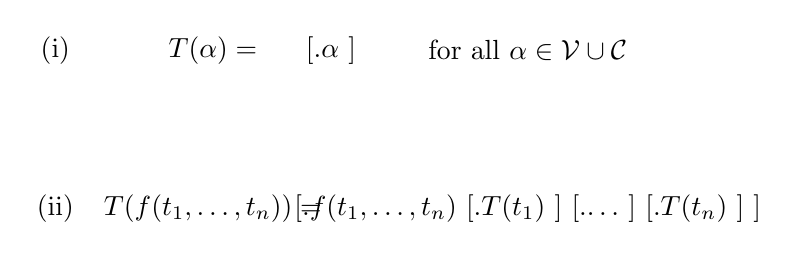
\begin{tikzpicture}
\node at (-2,1) {(i)};

\node at (0,1) {$T(\alpha)=$};
\node at (1.5,1) {\Tree [.$\alpha$ ]};
\node at (4,1) {for all $\alpha\in\mathcal{V}\cup\mathcal{C}$};

\node at (-2,-1) {(ii)};
\node at (0,-1) {$T(f(t_1, \mathellipsis,t_n))=$};
\node at (4,-1) {\Tree [.{$f(t_1, \mathellipsis,t_n)$} [.{$T(t_1)$} ] [.$\mathellipsis$ ] [.{$T(t_n)$} ] ]};

\end{tikzpicture}
\end{center}

		\item \emph{Examples}:
		
			\begin{enumerate}[(i)]
			
				\item Here's the parsing tree for the term $4=S(S(S(S(0))))$ in $\mathcal{L}_{PA}$:
				
				\begin{center}
				\Tree [.$S(S(S(S(0))))$ [.$S(S(S(0)))$ [.$S(S(0))$ [.$S(0)$ [.$0$ ] ] ] ] ]
				\end{center}
				
				\item Here's the parsing tree for $(2\cdot (2+1))=(S(S(0))\cdot (S(S(0))+S(0)))$
								
				\begin{center}
				\Tree [.$(S(S(0))\cdot (S(S(0))+S(0)))$ [.$S(S(0))$ [.$S(0)$ [.$0$ ] ] ] [.$(S(S(0))+S(0))$ [.$S(S(0))$ [.$S(0)$ [.$0$ ] ]  ] [.$S(0)$ [.$0$ ] ] ] ]
				\end{center}
				
				\item One last, more abstract example:
				
				\begin{center}
				\Tree [.{$f(g(a,b))$} [.$g(a,b)$ [.$a$ ] [.$b$ ] ] ]
				\end{center}
				
					\end{enumerate}

				
				\item We can now give the general, recursive definition of a parsing tree for a formula $\phi\in\mathcal{L}$:			
				
				\begin{center}
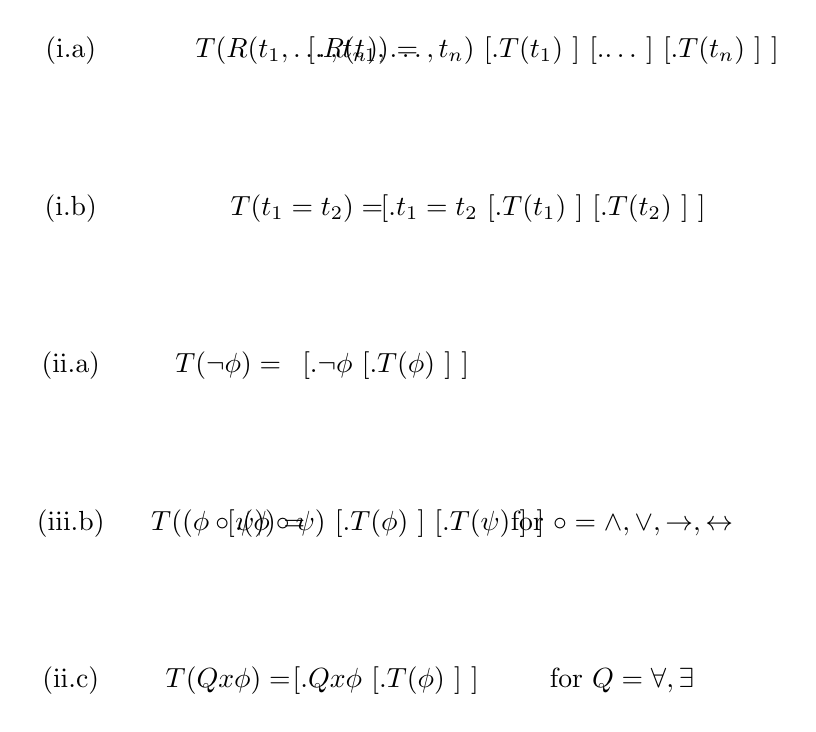
\begin{tikzpicture}
\node at (-2,1) {(i.a)};

\node at (1,1) {$T(R(t_1, \mathellipsis, t_n))=$};
\node at (4,1) {\Tree [.{$R(t_1, \mathellipsis,t_n)$} [.{$T(t_1)$} ] [.$\mathellipsis$ ] [.{$T(t_n)$} ] ]};

\node at (-2,-1) {(i.b)};
\node at (1,-1) {$T(t_1=t_2)=$};
\node at (4,-1) {\Tree [.$t_1=t_2$ [.$T(t_1)$ ] [.$T(t_2)$ ] ]};

\node at (-2,-3) {(ii.a)};
\node at (0,-3) {$T(\neg \phi)=$};
\node at (2,-3) {\Tree [.$\neg \phi$ [.$T(\phi)$ ] ]};

\node at (-2,-5) {(iii.b)};
\node at (0,-5) {$T((\phi\circ\psi))=$};
\node at (2,-5) {\Tree [.$(\phi\circ\psi)$ [.$T(\phi)$ ] [.$T(\psi)$ ] ]};
\node at (5,-5) {for $\circ=\land,\lor,\to,\leftrightarrow$};


\node at (-2,-7) {(ii.c)};
\node at (0,-7) {$T(Qx \phi)=$};
\node at (2,-7) {\Tree [.$Qx\phi$ [.$T(\phi)$ ] ]};
\node at (5,-7) {for $Q=\forall,\exists$};


\end{tikzpicture}
\end{center}
			
	
	  \item \emph{Example}. Since the idea of how to do parsing trees should be clear by now,
		we do just one, more involved example:
	
	\begin{center}
	
	\Tree [.{$\forall x(R(x,g(f(a),f(b)))\to \exists yR(y,y))$} [.{$R(x,g(f(a),f(b)))\to \exists yR(y,y)$} [.{$R(x,g(f(a),f(b)))$} [.$x$ ] [.{$g(f(a),f(b))$} [.$f(a)$ [.$a$ ]  ] [.$f(b)$ [.$b$ ]  ] ] ] [.$\exists yR(y,y)$ [.$R(y,y)$ [.$y$ ]  [.$y$ ] ] ] ] ]
	
	\end{center}
	
	\item At this point, we simply remark that it is now a straight-forward exercise to prove a Unique Readability Theorem for terms and formulas in first-order logic along the lines of the proof we gave in 4.3.8. Stating and proving this theorem is useful exercise.
			
	\item In the following, we shall need, for technical reasons, the notion of a \emph{stripped} parsing tree. The stripped parsing tree of a formula is the result of leaving only the main operator on each node when we're doing the ordinary parsing tree. Here is an explicit, recursive definition of stripped parsing trees for terms and formulas:\\[2ex]
	
\emph{Terms}:\\[2ex]
\begin{center}
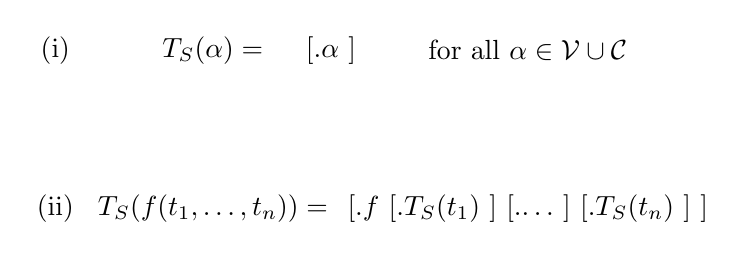
\begin{tikzpicture}
\node at (-2,1) {(i)};

\node at (0,1) {$T_S(\alpha)=$};
\node at (1.5,1) {\Tree [.$\alpha$ ]};
\node at (4,1) {for all $\alpha\in\mathcal{V}\cup\mathcal{C}$};

\node at (-2,-1) {(ii)};
\node at (0,-1) {$T_S(f(t_1, \mathellipsis,t_n))=$};
\node at (4,-1) {\Tree [.{$f$} [.{$T_S(t_1)$} ] [.$\mathellipsis$ ] [.{$T_S(t_n)$} ] ]};

\end{tikzpicture}
\end{center}	
	
\emph{Formulas}:\\[1ex]
\begin{center}
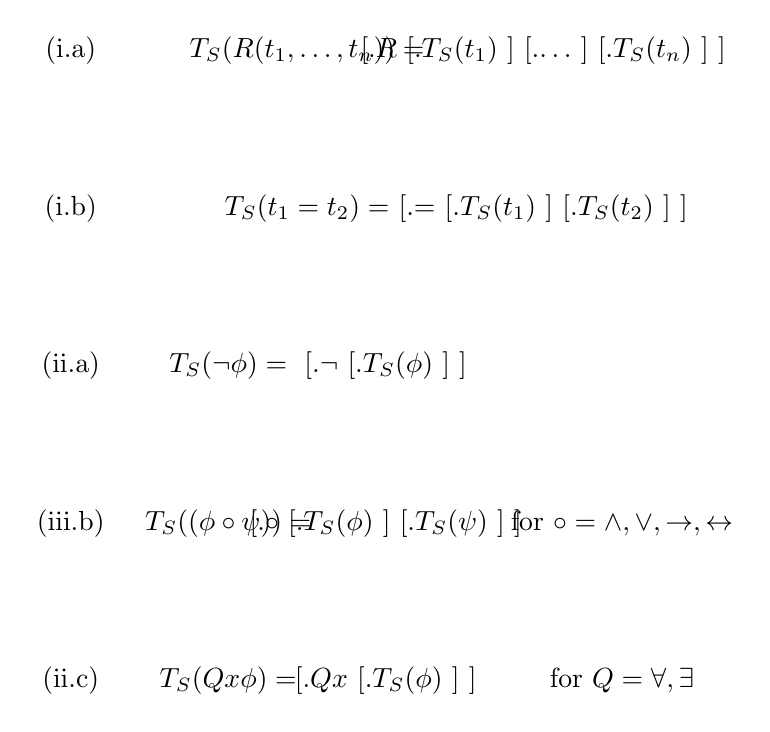
\begin{tikzpicture}
\node at (-2,1) {(i.a)};

\node at (1,1) {$T_S(R(t_1, \mathellipsis, t_n))=$};
\node at (4,1) {\Tree [.{$R$} [.{$T_S(t_1)$} ] [.$\mathellipsis$ ] [.{$T_S(t_n)$} ] ]};

\node at (-2,-1) {(i.b)};
\node at (1,-1) {$T_S(t_1=t_2)=$};
\node at (4,-1) {\Tree [.$=$ [.$T_S(t_1)$ ] [.$T_S(t_2)$ ] ]};

\node at (-2,-3) {(ii.a)};
\node at (0,-3) {$T_S(\neg \phi)=$};
\node at (2,-3) {\Tree [.$\neg$ [.$T_S(\phi)$ ] ]};

\node at (-2,-5) {(iii.b)};
\node at (0,-5) {$T_S((\phi\circ\psi))=$};
\node at (2,-5) {\Tree [.$\circ$ [.$T_S(\phi)$ ] [.$T_S(\psi)$ ] ]};
\node at (5,-5) {for $\circ=\land,\lor,\to,\leftrightarrow$};


\node at (-2,-7) {(ii.c)};
\node at (0,-7) {$T_S(Qx \phi)=$};
\node at (2,-7) {\Tree [.$Qx$ [.$T_S(\phi)$ ] ]};
\node at (5,-7) {for $Q=\forall,\exists$};


\end{tikzpicture}
\end{center}
In a sense, the information provided by the stripped parsing tree is the same as the information provided by the ordinary parsing tree: they both tell us how the formula was constructed.  In fact, it's easy to write an algorithm that translates an ordinary parsing tree into a stripped one and vice versa (exercise?). The difference between the two concepts is a difference in focus: while the ordinary parsing tree focuses on the information from which \emph{sub-formulas} a formula was constructed, the stripped parsing tree focuses on the \emph{operations} used along the way. Having easy access to this information will be useful along the way.

	\item \emph{Example}. Here's the stripped parsing tree for Example 8.3.5:
	
	\begin{center}
	
	\Tree [.{$\forall x$} [.{$\to$} [.{$R$} [.$x$ ] [.{$g$} [.$f$ [.$a$ ]  ] [.$f$ [.$a$ ]  ] ] ] [.$\exists y$ [.$R$ [.$y$ ]  [.$y$ ] ] ] ] ]
	
	\end{center}
	
	  \item In the following, we shall often need to access the information provided by parsing trees.
		In order to be able to do so, we need to be able to refer to the nodes in a given tree in a clear fashion.
		For this purpose, we introduce the following (standard!) naming  conventions for nodes in trees.
		Let me introduce the idea by means of an example.
		Take the tree:
		\begin{center}
		\Tree [.$\bullet$ [.$\bullet$  [.$\bullet$ [.$\bullet$ ] ] [.$\bullet$ [.$\bullet$ ] [.$\bullet$ ] ] ] ]
		\end{center}
		
		We then name nodes in this tree as follows:
		\begin{itemize}
		  \item%
			The root is always called $r$.
		  \item%
			The first child of the root is called $( r, 1)$.
		  \item%
			The first child of $( r, 1)$ is called $( r, 1, 1)$.
		  \item%
			The \emph{second} child of $( r, 1)$ is called $(r, 1, 2)$.
		  \item%
			\dots
		\end{itemize}
		So, the nodes in our tree are: \[r, (r,1), ( r,1,1), ( r,1,2),( r,1,1, 1), ( r,1,2,1) , ( r,1,2,2).\]
		Note that there can be empty names for nodes.
		For example, the node $(r,2,1,1)$ doesn't denote a node in our tree.

		Essentially, we name a node by giving the ``directions'' for someone traveling along the edges through the nodes.\footnote{%
		For interested: the naming of the nodes depends on how we draw the tree, but we'll ignore this complication.}
		Here is a more general, recursive (!) definition of the name $\ulcorner n\urcorner$ of a node $n$ in a tree:
		\begin{itemize}
		  \item%
			The name of the root is $r$
		  \item%
			The name of the $i$-th child of node $n$ is called $(\ulcorner n\urcorner, i)$.\footnote{%
			For this to look nice, we have to ``forget'' a bunch of parentheses in $\ulcorner n\urcorner$ according to the rule $((x,y),z)=(x,y,z)$.}

			This definition allows you to step-by-step calculate the name of a node in a tree.
		\end{itemize}

	\item We shall now define the central notion of an \emph{occurrence} of an expression in a formula. Intuitively, it's pretty clear what it means for an expression to occur in a formula: an expression occurs in a formula if you need to write it down in order to write the formula. So, for example, $P(x)$ occurs in $\forall x(P(x)\lor R(x,x))$. But for our intents and purposes, this intuitive notion doesn't provide enough information. We need better access to the internal structure of the formula. We get it, via the parsing tree. First, we shall give a precise definition of the notion of an occurrence:
	
	\begin{itemize}
	
		\item An expression $\sigma$ \emph{occurs} in a term or formula $\tau$ iff $\sigma$ is the label of some node in the (ordinary or stripped) parsing tree of $\tau$.
	
	\end{itemize}

	\item Let's begin with some examples:
	
		\begin{enumerate}[(i)]	
	
	
			\item The term $S(S(0))$ occurs in the term $S(S(S(S(0))))$, since it labels the node $(r,1,1)$ in the parsing tree:
\begin{center}
				\Tree [.$S(S(S(S(0))))$ [.$S(S(S(0)))$ [.$S(S(0))$ [.$S(0)$ [.$0$ ] ] ] ] ]
				\end{center}

			\item The quantifier $\exists y$ occurs in the formula $\forall x(R(x,g(f(a),f(b)))\to \exists yR(y,y))$ since it labels the node $(r,1,2)$ in the stripped tree:
	\begin{center}
	
	\Tree [.{$\forall x$} [.{$\to$} [.{$R$} [.$x$ ] [.{$g$} [.$f$ [.$a$ ]  ] [.$f$ [.$a$ ]  ] ] ] [.$\exists y$ [.$R$ [.$y$ ]  [.$y$ ] ] ] ] ]
	
	\end{center} 


		  \item The formula
			$R(x,y)$
			occurs \emph{twice} in the formula
			$\forall x(R(x,y)\to \exists x\forall y(R(y,x)\land \neg R(x,y)))$,
			once at
			$(r,1,1)$
			and once at
			$(r,1,2,1,1,2,1)$:
\begin{center}
\begin{tabular}{c}
{\Tree [.$\forall x(R(x,y)\to \exists x\forall y(R(y,x)\land \neg R(x,y)))$
		[.$R(x,y)\to \exists x\forall y(R(y,x)\land \neg R(x,y))$ 
			[.$R(x,y)$ [.$x$ ] [.$y$ ] ]
			[.$\exists x\forall y(R(y,x)\land \neg R(x,y))$ 
				[.$\forall y(R(y,x)\land \neg R(x,y))$ 
					[.$R(y,x)\land \neg R(x,y)$ 
						[.$R(y,x)$
							[.$y$ ]
							[.$x$ ]
						]	
						[.$\neg R(x,y)$ 
							[.$R(x,y)$
								[.$x$ ]
								[.$y$ ]
							]
						]
					]
				]
			]
		]
	]
}
\end{tabular}
\end{center}

\end{enumerate}

	  \item The fact that an expression can occur more than once requires us to talk about \emph{occurrences} of expressions.
		For many purposes we want to be able to \emph{distinguish} different occurrences of expressions, we want, for example, to be able to distinguish the occurrence of
		$R(x,y)$ at $(r,1,1)$
		from the occurrence at
		$(r,1,2,1,1,2,1)$.
		We do this by defining an \emph{occurrence} of an expression in a formula as the pair $(n,\sigma)$ where $n$ is a node in the parsing tree labelled with $\sigma$.
	
	\item \emph{Examples}. Consider the formula $\forall x(R(x,y)\to \exists x\forall y(R(y,x)\land \neg R(x,y)))$. We gave the ordinary parsing tree above. Here is the stripped one:
	\begin{center}
\begin{tabular}{c}
{\Tree [.$\forall x$
		[.$\to$ 
			[.$R$ [.$x$ ] [.$y$ ] ]
			[.$\exists x$ 
				[.$\forall y$ 
					[.$\land$ 
						[.$R$
							[.$y$ ]
							[.$x$ ]
						]	
						[.$\neg$ 
							[.$R$
								[.$x$ ]
								[.$y$ ]
							]
						]
					]
				]
			]
		]
	]
}
\end{tabular}
\end{center}
	
		\begin{itemize}
		
			\item The following are all the occurrences of logical operators in the formula:
			
				\begin{longtable}{l}
					$(r,\forall x)$\\
					$((r,1),\to)$\\
					$((r,1,2),\exists x)$\\
					$((r,1,2,1),\forall y)$\\
					$((r,1,2,1,1),\land)$\\
					$((r,1,2,1,1,2),\neg)$
				\end{longtable}

				
			\item The following are all the occurrences of predicate symbols in the formula:
				
				\begin{longtable}{l}
					$((r,1,1),R)$\\
					$((r,1,2,1,1,1),R)$\\
					$((r,1,2,1,1,2,1),R)$
				\end{longtable}

			\item The following are all the occurrences of variables in the formula:
				
				\begin{longtable}{l}		
					$((r,1,1,1),x)$\\
					$((r,1,1,2),y)$\\
					$((r,1,2,1,1,1,1),y)$\\
					$((r,1,2,1,1,1,2),x)$\\
					$((r,1,2,1,1,2,1,1),x)$\\
					$((r,1,2,1,1,2,1,2),y)$
				\end{longtable}
				
				\item The following are all the occurrences of formulas in the formula:
				\begin{longtable}{l}		
					$(r,\forall x(R(x,y)\to \exists x\forall y(R(y,x)\land \neg R(x,y))))$\\
					$((r,1),(R(x,y)\to \exists x\forall y(R(y,x)\land \neg R(x,y))))$\\
					$((r,1,1),R(x,y))$\\
					$((r,1,2),\exists x\forall y(R(y,x)\land \neg R(x,y))))$\\
					$((r,1,2,1),\forall y(R(y,x)\land \neg R(x,y)))$\\
					$((r,1,2,1,1),(R(y,x)\land \neg R(x,y)))$\\
					$((r,1,2,1,1,1),R(y,x))$\\
					$((r,1,2,1,1,2),\neg R(x,y))$\\
					$((r,1,2,1,1,2,1),R(x,y))$\\
					
				\end{longtable}
				
				
			\end{itemize}

\end{enumerate}

\section{Free and Bound Variables}

	\begin{enumerate}[\thesection.1]

		%\item With the technical concepts from the previous section in place, we can now study the internal, quantificational structure of first-order formulas. We're essentially going to study how to understand first-order formulas with only the intuitive ideas laid out in 8.1 in mind.
		
		\item Variables, just like pronouns are tricky. They allow us to talk about things in general, to say things like ``everything that's scarlet is red'' in a logically precise fashion; but, at the same time, it's not always easy to figure out what your variables refer to, especially when you have more than one variable around. Take the formula $\forall x\exists yR(x,y)$, for example. If we read $R$ as ``\dots is smaller than \underline{\phantom{\dots}}'' and assume that we're only talking about numbers, then this statement says that for every number there is a number bigger than it. Now, how can you see that the ``it'' refers to the first number that we talked about and not the second? This information is encoded in the \emph{quantificational structure} of the formula: which quantifier talks about which variable. In this section, we set out to understand this structure.
		
		\item The concept that we're trying to understand is that of a quantifier \emph{capturing} a variable. The idea is as follows. Take the formula: \[\forall x(P(a)\land \neg R(x,a)).\] In this formula, the universal quantifier $\forall x$ stands at the very beginning, but clearly it ``captures'' the variable $x$ later on in the formula. So, if, for example, $a$ stands for Socrates, $P$ for ``\dots is a philosopher,'' and $R$ stands for ``\dots is a friend of \underline{\phantom{\dots}},'' then the formula should read: everybody is such that Socrates is a philosopher and they are not a friend of Socrates; or, more perspicuously, Socrates is a philosopher and nobody is his friend (\frownie). The point is this. For a quantifier to capture a variable, $x$, clearly the quantifier needs to talk about the variable, i.e. it needs to be of the form $\forall x$ or $\exists x$. But it does not need to stand immediately in front of the predicate the variable is applied to, as in $\forall xP(x)$; no, it can be farther away as in our example. 
		
		\item But is it enough for a quantifier to capture a variable that the quantifier talks about the variable and occurs before it in the formula? The answer is no. Take the formula $\forall x(\exists y \neg R(x,y)\lor (P(x)\to R(c,y)))$. Here are its ordinary and stripped parsing trees:
		\begin{center}
\begin{tabular}{ccc}
\Tree [.{$\forall x(\exists y \neg R(x,y)\lor (P(x)\to R(c,y)))$} [.{$(\exists y\neg R(x,y)\lor (P(x)\to R(c,y)))$} [.{$\exists y\neg R(x,y)$} [.{$\neg R(x,y)$} [.$R(x,y)$ [.$x$ ] [.${y}$ ] ] ] ] [.$(P(x)\to R(c,y))$ [.$P(x)$ [.$x$ ] ] [.$R(c,y)$ [.$c$ ] [.${y}$ ] ] ] ] ]

&\quad&

 \Tree [.{$\forall x$} [.$\lor$ [.{$\exists y$} [.$\neg$ [.$R$ [.${x}$ ] [.{$y$} ] ] ] ] [.$\to$ [.$P$ [.${x}$ ] ] [.$R$ [.$c$ ] [.{$y$} ] ] ] ] ]

\end{tabular}
\end{center}
In this formula, there is an occurrence of the variable $y$ at $(r,1,2,2,2)$, which is written in the formula after the quantifier $\exists y$ at $(r,1,1)$. But we should think that the quantifier does not bear the right relation to the variable since when we look at the way the formula was constructed the variable $y$ at $(r,1,2,2,2)$ wasn't even around when $\exists y$ at $(r,1,1)$ was introduced. So how could it ``capture'' the variable if it wasn't even there yet. 

A natural answer would be that a quantifier needs to be ``connected'' to the variable in the right way, i.e. by means of a path in the parsing tree. Take the occurrence of $y$ at $(r,1,1,1,1,2)$. This variable \emph{was} around when $\exists y$ at $(r,1,1)$ was introduced. In fact, we can see this by tracing a path from $y$ at $(r,1,1,1,1,2)$ to $\exists y$ at $(r,1,1)$. This gives us a second condition for a quantifier to capture a variable: in addition to the quantifier talking about the variable, there needs to be a path from the variable to the quantifier in the parsing tree. Is this enough?
	
	\item It turns out, the answer is no! This might be surprising but there is one phenomenon that we haven't properly taken into account yet. Take the formula $\forall x({N}(x)\to {\exists x}R(x,x))$. Here are the parsing trees:
\begin{center}
	
		\begin{tabular}{c c c}
	
	\Tree [.$\forall x({N}(x)\to {\exists x}R(x,x))$ [.${N}(x)\to \exists x{R(x,x)}$ [.${N}(x)$ [.$x$ ] ] [.${\exists x}R(x,x)$ [.$R(x,x)$ [.$x$ ] [.$x$ ] ] ] ] ]

	&\quad &
	
	\Tree [.$\forall x$ [.$\to$ [.${N}$ [.$x$ ] ] [.${\exists x}$ [.$R$ [.$x$ ] [.$x$ ] ] ] ] ]

	
	\end{tabular}
	\end{center}
	
	
	 If we read $N$ as ``\dots is a natural number'' and $R$ as ``\dots is smaller than or equal to \underline{\phantom{\dots}},'' then what this formula says is that for all numbers, there is a number that is smaller than or equal to itself. This statement is a bit artificial, but I hope the point is clear: the first quantifier $\forall x$ only talks about the first occurrence of $x$ at $(r,1,1,1)$. The second and third occurrence of $x$ at $(r,1,2,1,1)$ and  $(r,1,2,1,2)$ respectively, are captured by $\exists x$ at $(r,1,2)$. You can see this in the way we read the consequent of the conditional: $\exists x R(x,x)$ says that there exists a number that is smaller than or equal to itself. There is no remaining, unclear pronoun which is there for $\forall x$ to capture. This consideration gives us the final condition for a quantifier to successfully capture a variable: there cannot be another quantifier that captures the variable first. 
	
	\item Putting this all together, we get to the following official definition of a quantifier occurrence capturing or, as we typically say in logic, \emph{binding} a variable occurrence:
	
	\begin{itemize}
		
		\item Let $( n, x)$ be an occurrence of a variable $x$ in a formula $\phi$ and $( m, Qy)$ an occurrence of a quantifier $Q=\forall,\exists$ in $\phi$. Then, $( n, x)$ is {\it bound} by  $( m, Qy)$ iff
\begin{enumerate}[(i)]
\item $x=y,$
\item there is an downwards path from $m$ to $n,$
\item this path from $m$ to $n$ does not go through a node $k$ such that $( k, Q'x)$ is an occurrence of a quantifier $Q'=\forall,\exists$ in $\phi$.

\end{enumerate}
When a variable occurrence in a formula is not bound by some quantifier occurrence in the same formula, we also call the variable occurrence \emph{free}.

	\end{itemize}
	
	\item \emph{Examples}. Let's consider some examples.
	
		\begin{enumerate}[(i)]
		
			\item For the variable occurrence $((r,1,2,2,2), y)$ in $\forall x(\exists y \neg R(x,y)\lor (P(x)\to R(c,y)))$ and the quantifier occurrence $((r,1,1),\exists y)$ in the same formula, the condition (ii) is violated. For occurrence $(r,1,1,1,1,2)$, instead, we're good: $((r,1,1),\exists y)$ binds $(r,1,1,1,1,2)$. 
		
			\item We've just seen that for the variable occurrences $((r,1,2,1,1),x)$ and  $((r,1,2,1,2),x)$ in $\forall x(N(x)\to \exists xR(x,x))$, only the quantifier occurrence $((r,1,2),\exists x)$ binds them. Occurrence $(r,\forall x)$ does not bind either because condition (iii) of Definition 8.4.5 is violated. 
	
			\item The following table has the information which variable occurrence is bound by which quantifier occurrence in the formula $\forall x(R(x,y)\to \exists x\forall y(R(y,x)\land \neg R(x,y)))$ from Example 8.2.13
	
	\begin{center}
	\begin{tabular}{ c | c }
				Variable occurrence & Quantifier occurrence\\\hline
		
			$( ( r,1,1,1), x)$ & $( r, \forall x)$ \\
			$( ( r,1,2,1,1,1,1), y)$ & $( ( r,1,2,1), \forall y)$ \\
			$( ( r,1,2,1,1,1,2), x)$ & $( ( r,1,2), \exists x)$ \\
			$( ( r,1,2,1,1,2,1,1), x)$ & $( ( r,1,2), \exists x)$\\
			$( ( r,1,2,1,1,2,1,2), y)$ & $( ( r,1,2,1), \forall y)$\\
		
		\end{tabular}
		\end{center}
		
		\end{enumerate}
	
		\item Now, with the notion of variable binding in place, we can define the central concept of open and closed formulas: we say that a formula is \emph{open} iff there exists a variable occurrence in the formula that is not bound by some quantifier occurrence in the same formula. A formula is called \emph{closed} iff it's not open, i.e. iff all variable occurrences in the formula are bound by some quantifier occurrence. 
	
		\item \emph{Examples}: Let's first look at our examples:
		
		
			\begin{itemize}
			
				\item $\forall x(R(x,y)\to \exists x\forall y(R(y,x)\land \neg R(x,y)))$ is open, since $((r,1,1,2),y)$ is free.

			
				\item $\forall x(\exists y \neg R(x,y)\lor (P(x)\to R(c,y)))$ is open since $( ( r,1,2,2,2), y)$ is free
				
				\item $\forall x({N}(x)\to {\exists x}R(x,x))$ is closed.
			
			\end{itemize}

	  \item In the following, we shall study only inferences involving closed formulas or \emph{sentences} as they are typically called.
		The reason for this is that open formulas are not straight-forwardly apt to be true or false in a possible situation: an open formula, like $P(x)$, contains an unbound variable, which intuitively is something like a pronoun who's reference you don't know.
		This spells trouble for our account of valid inference.
		Suppose that somebody comes into the room and declares ``She's coming! So, we should all be happy.''
		How can you possibly determine any relation between the truth of ``she's coming'' and ``we should all be happy'' without knowing who ``she'' refers to?
		It \emph{is} possible to use free variables and (disambiguated) pronouns in a reasonable, logical way.
		For example, in mathematics, we often write an open formula
		$x+y=y+x$
		to express a general claim about all numbers, rather than using the universally quantified sentence
		$\forall x\forall y(x+y=y+x)$
		for the same purpose.
		Similarly, we reasonably reason from ``he's coming'' to ``he's not not coming;'' we don't need to know who ``he'' is for that purpose.
		But, it turns out that if we consider valid inferences between open formulas, all sort of technical difficulties pop up (they're not unsurmountable, but they're there).
		To avoid these problems, we'll focus on inferences between sentences alone.
		This is actually not that much of an restriction since we'll have to think about the truth-conditions for open formulas anyways when we try to give truth-conditions for sentences.
		Why you can already see now from a purely syntactic standpoint:
		sentences, like
		$\forall xP(x)$,
		are constructed from open formulas,
		in this case $P(x)$;
		so, if we want to trace the construction of a formula in our recursive definition of truth, we need to give the truth-conditions for the open formula
$P(x)$.
		\item It is worth, as an exercise, to prove some basic facts about free and bound variable. Here we report some propositions, leaving most of the proofs as exercises, however:
		
		\begin{proposition}
		Let $x$ be a variable and $\phi,\psi$ formulas. Then:
		\begin{enumerate}[1.]
		
			\item If $x$ occurs free in $\phi$, then $x$ occurs free in $\neg\phi$
			
			\item If $x$ occurs free in either $\phi$ or $\psi$, then $x$ occurs free in $(\phi\circ\psi)$ for $\circ=\land,\lor,\to,\leftrightarrow$
			
			\item If $x$ occurs free in $\phi$ and $y\neq x$, then $x$ occurs free in $Qy\phi$ for $Q=\forall,\exists$.
		
		\end{enumerate}
		\end{proposition}
		\begin{proof}
		We only proof 3. Suppose that $x$ occurs free in $\phi$, at $(n,x)$, and $y\neq x$. Suppose further, for contradiction, $(n,x)$ is bound by some occurrence $(k,Q'x)$ of quantifier $Q'x$, $Q'=\forall,\exists$, in $Qy\phi$. Clearly, $k$ can't be $r$, i.e. the root of the stripped parsing tree for $Qy\phi$. Why? Well, since there we find $Qy$ and by assumption $x\neq y$. So, for $(r,Qy)$, condition (i) of Definition 8.4.5 is violated, meaning $(r,Qy)$ can't bind any occurrence of $x$. But since the (stripped) parsing tree for $Qy\phi$ looks as follows, 		
		\begin{center}
		\Tree [.$Qy$ [.$T_S(\phi)$ ] ]
		\end{center}
This means that $k$ must be a node in $T_S(\phi)$. But that would mean that $(k,Q'x)$ binds $(n,x)$ in $\phi$. Contradiction. Hence $(n,x)$ is also free in $Qy\phi$, as desired.

		\end{proof}

	\end{enumerate}
	
\section{Substitution}

	\begin{enumerate}[\thesection.1]

		\item Before we talk about formalization, we will introduce the concept of \emph{substitution} of terms for (free) variables in formulas. The point of this operation is to be able, in a purely syntactic way, to specify what certain pronouns stand for. Remember that in first-order logic, we treat pronouns as variables: ``it is red,'' for example, is formalized as $R(x)$. Now, without knowing what ``it'' stands for, we cannot determine whether this sentence is true or false. In semantics, which we treat in the next chapter, we will discuss a semantic way of achieving this. But for many purposes, especially proof theory, it will be useful to be able to do this in a purely syntactic fashion, i.e. just by manipulating symbols. This is what the operation of term-substitution allows us to do. To illustrate the idea, think of the sentence ``it is red'' formalized as $R(x)$ again. Suppose further that in our language we refer to the ball using the constant $a$. A simple way of making it explicit that ``it'' stands for the ball is to replace the $x$ in $R(x)$ with $a$ to get $R(a)$, a formula that says that the ball is red. We will now define this operation as a general operation on formulas: the operation of a term substituting a term $t$ for free occurrences of a variable $x$ in a formula $\phi$. For this, we write $(\phi)[x:=t]$.
			
		\item In order to be able to define the operation, we first need to define what it means to replace a term for a variable in another term. This is because variables can be nested somewhere in functional expressions, such as $f(a, g(h(x),c))$. To handle this, we define the operation $(s)[x:=t]$ of replacing a term $t$ for a variable $x$ in another term $t$ recursively as follows:
		
			\begin{enumerate}[(i)]
			
				\item $(s)[x:=t]=\begin{cases} s & \text{if } s\neq x\\ t & \text{ if }s=x\end{cases}$ for $s\in \mathcal{C}\cup\mathcal{V}$
				
				\item $(f(t_1,\mathellipsis, t_n))[x:=t]=f((t_1)[x:=t], \mathellipsis, (t_n)[x:=t])$
			
			\end{enumerate} 
			
	Note the parentheses which indicate the \emph{scope} of the substitution operation: where to apply the operation. Let's go through one example step-by-step, let's calculate $(f(a, g(h(x),c)))[x:=c]$:
	
	\begin{align*}
	(f(a, g(h(x),c)))[x:=c]&=f((a)[x:=c], (g(h(x),c))[x:=c])\\
	&=f(a, g((h(x))[x:=c], (c)[x:=c]))\\
	&=f(a,g(h((x)[x:=c]), c)\\
	&=f(a,g(h(c),c))
	\end{align*}
Well, we could have done this without the recursive definition, sure. But the point here is that we want all of our definitions to be, at least in principle, computer implementable---and the way we can achieve this is by defining them properly, recursively.

	\item	Now we can define the notion $(\phi)[x:=t]$ of substituting $t$ for all free occurrences of $x$ in $\phi$. We do this recursively:	
		\begin{enumerate}[(i)]
	
			\item \begin{enumerate}[(a)] 
			
				\item $(R(t_1, \mathellipsis, t_n))[x:=t]=R((t_1)[x:=t], \mathellipsis, (t_n)[x:=t])$
				
				\item $(t_1=t_2)[x:=t]=t_1[x:=t]=t_2[x:=t]$
				
			\end{enumerate}
			
			\item \begin{enumerate}[(a)] 

			\item $(\neg\phi)[x:=t]=\neg((\phi)[x:=t])$

			
			\item $((\phi\circ\psi))[x:=t]=((\phi)[x:=t]\circ(\psi)[x:=t])$ for $\circ=\land,\lor,\to,\leftrightarrow$
			
			\item $(Qy\phi)[x:=t]=\begin{cases} Qy(\phi)[x:=t] & \text{if } y\neq x\\ Qy\phi & \text{if }y=x\end{cases}$ for $Q=\forall,\exists$

			\end{enumerate}
	

			\end{enumerate}
			
	The crucial clause is (ii.c), which blocks us from substituting the variable as soon as we hit upon a quantifier that binds it. This is because we only want to replace \emph{free} occurrences of variables. Why? Well, first of all, because only for free variables it's unclear what they stand for. So only for them do we need to use substitution to say what they stand for. Moreover, if we replaced bound variables, we could change the meaning of statements. To see this, note that $\exists xR(x)$ says that there exists a red thing (assuming that $R$ stands for ``\dots is red''). Now, suppose that $(\exists xR(x))[x:=a]$ would yield $\exists xR(a)$. This would turn the statement ``there exists a red thing'' into the statement ``there exists an object such that the ball is red'' (assuming that $a$ stands for the ball). This is not only a weird statement, it could actually be false, even if ``there exists a red thing'' is true: suppose that the ball is blue and the cup is red. Then ``there exists a red thing'' is true but ``there exists an object such that the ball is red''  is false. \frownie
	
	\item \emph{Example}. Here is a step-by-step calculation of the result of a substitution: 
	
	$(\forall x(\exists y \neg R(x,y)\lor (P(x)\to R(c,y))))[y:=c]$
	\begin{align*}
	&=\forall x((\exists y \neg R(x,y)\lor (P(x)\to R(c,y))))[y:=c]\\
	&=\forall x(((\exists y \neg R(x,y)))[y:=c]\lor ((P(x)\to R(c,y)))[y:=c])\\
	&=\forall x((\exists y \neg R(x,y))\lor ((P(x))[y:=c]\to (R(c,y))[y:=c]))\\
	&=\forall x((\exists y \neg R(x,y))\lor (P((x)[y:=c])\to (R((c)[y:=c]), (y)[y:=c])))\\
	&=\forall x(\exists y \neg R(x,y)\lor (P(x)\to R(c,c)))
	\end{align*}
	
	%\item We conclude our discussion of substitution with a ``sanity check'' for our definition: we'll prove that if we replace a term for a variable in a formula 
	
%	\item To deepen our understanding of substitution, let's prove one characteristic proposition:
%	
%	\begin{lemma}
%	Let $x$ be a variable that occurs free in $\phi$ and $y$ any other variable. Then $y$ occurs free in $\phi[x:=y]$. 
%	\end{lemma} 
%	\begin{proof}
%	
%	
%	\end{proof}
	
	\end{enumerate}
	
\section{Formalization}

	\begin{enumerate}[\thesection.1]
	
		\item We conclude this chapter with a brief discussion of formalization in first-order logic. All the points from propositional logic still apply. The translation key in first-order logic contains the following information:
		
		\begin{enumerate}[(i)]
		
			\item A so-called \emph{domain of discourse}, $D$, which is the set of things we're talking about.
			
			\item For each constant in the signature, a natural language term it formalizes.
			
			\item For each predicate in the signature, a natural language predicate it formalizes.
			
			\item For each function symbol in the language, a natural language expression it formalizes.
			
		\end{enumerate}
	So, bottom-line, the translation key gives us the reading of the vocabulary in the signature.
	
	\item \emph{Examples}. 
	
		\begin{enumerate}[(i)]
		
		\item Here is an example of the standard translation key for $\mathcal{L}_{PA}$:
		
			\begin{itemize}
		
				\item $D=\mathbb{N}$
				
				\item $0$: the number 0
				
				\item $S$: the successor function which maps every number $n$ to the next biggest number
				
				\item $+$: addition
				
				\item $\cdot$ : multiplication
		
			\end{itemize}
			
		  \item Here's a(n arbitrary) translation key for our abstract signature $\mathcal{S}=(\{a,b,c\}, \{f^1, g^2\}, \{P^1, R^2\})$:
			
			\begin{itemize}
			
				\item $D=\{x:x \text{ is a human}\}$
        
				\item $f$: the function that maps a person to their mother
				
				\item $g$: the function that maps two people to their LCA
				
				\item $P$: being a philosopher
				
				\item $R$ : being taller than
			
			\end{itemize}
		
		\end{enumerate}
		
		\item Here are some standard translation patterns for existential quantifiers in natural language (``some,'' ``there exists,'' \dots) using any translation key where $S$ stands for ``\dots is smart'' and $H$ stands for ``\dots is handsome.''
		
		\begin{longtable}{p{6cm} c l}
		
		Somebody who's smart exists & $\leadsto$ & $\exists x S(x)$\\

		
		There's somebody who's not smart & $\leadsto$ & $\exists x\neg S(x)$\\

Somebody's smart and somebody's handsome & $\leadsto$ & $\exists xS(x)\land \exists xH(x)$\\

Somebody's smart and handsome & $\leadsto$ & $\exists x(S(x)\land H(x))$\\
 Nobody's both smart and handsome & $\leadsto$ &$\neg\exists x(S(x)\land H(x))$\\
 
 Somebody, who's smart, is handsome & $\leadsto$ & $\exists x(S(x)\land H(x))$
		
		\end{longtable}
		
		One \emph{very important} piece of advice: what you want to say is \emph{almost never} (!): \[\exists x(S(x)\to H(x)),\] i.e. someone is such that if they're smart, then they're handsome. Remember that $\to$ is the material conditional, so this statement would already be true if there's someone who's not smart (clear? if not, read 5.1.6 again); and it's only false if there is someone who's both smart and not handsome.
		
		
		\item Here are some standard translation patterns for universal quantifiers in natural language (``for all,'' ``every,'' \dots) using the same translation key as in the previous examples:		
		\begin{longtable}{p{6cm} c l}
		
		Not everybody handsome is smart & $\leadsto$ & $\neg\forall x(H(x)\to S(x))$\\
Everybody who's smart is handsome & $\leadsto$ &$\forall x(S(x)\to H(x))$\\
A person who's smart is handsome & $\leadsto$ &$\forall x(S(x)\to H(x))$\\
Someone who's smart is handsome & $\leadsto$ &$\forall x(S(x)\to H(x))$\\
Everybody's smart and handsome & $\leadsto$ &$\forall x(S(x)\land H(x))$
		\end{longtable}
		Note well, however, that $\forall x(S(x)\land H(x))$ and $\forall x(S(x)\to H(x))$ say \emph{very} different things: the former says everybody is both smart and handsome, while the latter says that everybody who's smart is also handsome.
		
		\item Indeterminate terms, like pronouns, indexicals, etc., are formalized using free variables. Only when clearly the same thing is meant, use the same variable, if different things could be meant, use different variables:
		
		\begin{longtable}{p{7cm} c l}
		He's handsome & $\leadsto$ & $H(x)$\\
		She's handsome and smart & $\leadsto$ & $H(x)\land S(x)$\\
		He's handsome and \emph{he}'s smart & $\leadsto$ & $H(x)\land S(y)$\\
		He's handsome and she's smart & $\leadsto$ & $H(x)\land S(y)$\\
		That's a smart and handsome person & $\leadsto$ & $H(x)\land S(x)$\\
		
		
		\end{longtable}
		
		\item[8.6.5.$\frac{1}{2}$] One last piece of advice on formalization with quantifiers. If you're unsure about the quantificational structure of a sentence, it's always a good idea to follow the method we used in 8.1.6, when we introduced the quantifiers. The idea is to first rephrase a quantified statement, i.e. a statement with a quantifier expression in it, using pronouns;  to replace those pronouns with variables (following the guideline that possibly different objects get different variables); and finally to abstract the whole statement. Here's another example. Take the statement ``Every number has a successor.'' To arrive at an adequate formalization, we proceed as follows:
		\begin{itemize}
		
			\item Every number has a successor.
			
			\item Every number is such that it has a successor.
			
			\item Every object is such that if it is a number, then it has a successor.
			
			\item Every object is such that if it is a number, then there exists an object such that it's the successor of the former number.
			
			\item Every $x$ is such that if $x$ is a number, then there exists an object $y$, such that $y$ is the successor of $x$.
			
			\item $\forall x(N(x)\to \exists y(S(x)=y))$
			
			\item[] Assuming that $N$ stands for ``\dots is a number,'' and $S$ expresses the successor function.
		
		\end{itemize}
		
		\item Last, we briefly discuss how we can express that there are a fixed number of objects with a certain property. Let's suppose that we want to say that there is at least one thing that has a certain property. If we use $P$ as a predicate for a property, a simple formula that will do the trick is \[\exists xP(x)\tag{Exists$_1$}\] Now, suppose that we want to say that there is \emph{at most} one object (possibly none). How can we do that? Well, a neat little mathematical idea (that we've already used in \S2 and in the context of functions, cf. 3.6.10) is to say that to say that at most one object is so-and-so is to say that any candidate so-and-so object is \emph{unique} in being so-and-so, meaning any other object that is also so-and-so is already our object: \[\forall x\forall y(P(x)\land P(y)\to x=y)\tag{At Most$_1$}\] If we want to say that there is \emph{precisely} one object that's so-and-so, we can easily achieve this by forming the conjunction of (Exists$_1$) and (At Most$_1$):\[\exists xP(x)\land \forall x\forall y(P(x)\land P(y)\to x=y)\] This formula can be a bit simplified as follows: \[\exists x(P(x)\land \forall y(P(y)\to x=y))\tag{Exactly$_1$}\] This is, essentially, the formulation that we standardly use in mathematics to say that there is precisely one $P$.
		
		\item Ok, so far so good. Now what if we want to say that there are at least \emph{two} things that are so-and-so. Well clearly there have to be two things, $x$ and $y$ that are both so-and-so. But is this enough? Well, no! The objects $x$ and $y$ could be identical, in which case there would be only one object after all. So, we need to exclude this possibility, which gives us the following natural formula for saying that there are at least two things:
		\[\exists x\exists y(P(x)\land P(y)\land x\neq y)\tag{Exists$_2$}\]
And what about \emph{at most} two things? Well, it shouldn't be possible that there are three things, any potential third thing would have to already be one of our initial two. So, generalizing the idea from (At Most$_1$), we get: \[\forall x\forall y\forall z(P(x)\land P(y)\land P(z)\to x=y\lor x=z\lor y=z)\tag{At Most$_2$}\]
So, to say that we have \emph{exactly} two $P$'s, we can just conjoin
(Exists$_2$) and (At Most$_2$):\[\exists x\exists y(P(x)\land
  P(y)\land x\neq y)\land \forall x\forall y\forall z(P(x)\land
  P(y)\land P(z)\to x=y\lor x=z\lor y=z)\] A somewhat more palatable
formula to the same effect is: \[\exists x\exists y(P(x)\land
  P(y)\land x\neq y\land \forall z(P(z)\to x=z\lor y=z))\tag{Exactly$_2$}\]
		
		Now, you hopefully see the pattern. Can you write a formula that says that there are at least/at most/exactly 3 $P$'s?

			\end{enumerate}

%Add sections on: identity, nested quantifiers, etc.

\section{Core Ideas}

	\begin{itemize}
	
		\item In first-order logic, we take the grammatical structure of simple sentences into account.
		
		\item  Singular terms stand for objects and predicates for properties/relations.
		
		\item Quantifiers allow us talk about things in generality.
		
		\item The signature of a language consists of a set of constants, a set of function symbols, and a set of predicate symbols (the latter two with a fixed arity assignment).
		
		\item Both terms and formulas are defined inductively in first-order logic.
		
		\item We have induction for formulas and terms and function recursion.
		
		\item Parsing trees are defined for terms and functions.
		
		\item Nodes in trees have a canonical way of being named: by the directions for how to find them starting at the root. 
		
		\item Variables are bound by quantifiers.
		
		\item A formula without free variables is closed, a
                  sentence.

                  \item Substitution is a useful syntactic operation
                    that allows us to say what a variable stands for.
		
		\item Just like in propositional logic, there are guidelines for formalization.
					
	\end{itemize}

\section{Self Study Questions}

\begin{enumerate}[\thesection.1]

\item Which of the following entails that an expression is \emph{not}
  a formula of a first-order language (of appropriate signature)?

\begin{enumerate}[(a)]
\item The expression contains a sentence letter.
\item The expression contains an even number of parentheses.
\item The expression contains a symbol not from the vocabulary.
\item The expression contains a variable occurrence that is not bound
  by any quantifier occurrence.
\item The expression contains an $n$-ary function symbol followed by
  $m$-terms for $m\neq n$.
\item The expression does not have a parsing tree.
\item The expression contains quantifier occurrences that don't bind
  any variable occurrences.
\item The expression contains an odd number of parentheses.  
\item The expression contains no sentential operators.
\end{enumerate}

\item Let $\phi$ be a formula,  $(n,x)$ be a variable occurrence in
  $\phi$ and $(m,Qy)$ a quantifier occurrence in $\phi$ such that
  $(n,x)$ is bound by $(m,Qy)$. Which of the following are \emph{not}
  possible?

\begin{enumerate}[(a)]
\item $y\neq x$
\item $n=r$
\item $m=r$
\item There is a path from $m$ to $n$ such that $Qy$ is on that path
  (for $Q=\exists,\forall$)
\item There is a path from the root to $n$ which does not go through
  $m$.
\item There is a path from the root to $m$ which goes through $n$.
\item There is a path from the root to $n$ which goes through $m$.
\item There is a path from the root to $m$ which does not go through $n$.
\end{enumerate}

  \item Let $\phi$ be a formula with precisely one free variable, $x$.
	Consider the result of a substitution $(\phi)[x:=t]$ of term $t$ \emph{without free variables}
	for all free occurrences of $x$ in $\phi$.
	Which of the following can\emph{not} happen?

\begin{enumerate}
\item $(\phi)[x:=t]$ is open.
\item $(\phi)[x:=t]$ is closed.
\item $(\phi)[x:=t]$ contains no variables.
\item $(\phi)[x:=t]$ does not contain $t$.
\item $(\phi)[x:=t]$ contains free occurrences of $x$
\item $(\phi)[x:=t]$ does not contain $x$
\item $(\phi)[x:=t]$ is an atomic formula
\end{enumerate}
  
\end{enumerate}


\section{Exercises}
	
	\begin{enumerate}[\thesection.1]
	
		\item $[h]$ Define the notion of a subformula in first-order logic by generalizing Definition 4.4.2.
		
		\item $[h]$ Prove that for each formula $\phi$, if $x$ is the only variable that occurs free in $\phi$, then $Q x\phi$ is closed for $Q=\forall,\exists$.
		
		\item \begin{enumerate}[(a)]
		
		\item Use syntactic recursion to define a function $FV:\mathcal{L}\to\wp(\mathcal{V})$, which maps a formula $\phi$ to the set $FV(\phi)$ of all the variables that occur free in $\phi$.
				
		\item Prove that $FV(Qx\phi)=FV(\phi)\setminus\{x\}$ using induction on formulas.
		
		\end{enumerate}
		
		\item Adapt the algorithm from 4.3.10 to first-order logic.
		
		\item Prove 1. and 2. of 8.4.10.
		
		\item $[h]$ Is it the case that every sub-formula of a sentence is itself a sentence? If so, prove it. If not, give a counterexample.
		
		\item Let $x$ be a variable that occurs free in $\phi$ and $y$ any other variable. Is it always the case that $y$ occurs free in $\phi[x:=y]$? If so, prove it. If not, provide a counter-example.
		
		\item Do the parsing trees for  \[\forall x((R(x,x)\land \exists yR(z,y))\to \exists x\forall zB(x,x,y)).\] Determine all the occurrences of quantifiers and variables in the formula. For each occurrence of a variable determine if it's free or bound. If it's bound, determine which occurrence of a quantifier binds it.
			
		\item Step-wise calculate the results of the following substitutions.
		
		\begin{enumerate}[(i)]

			\item $[h]$ $(\forall x(R(x,y)\to\exists yR(y,y)))[y:=x]$


			\item $\forall x(P(x)\lor (\exists y(R(y,x)\to \neg Q(x)))[x:=c])$

			\item $(\forall z(R(z,z)\to (\neg R(z,z)\leftrightarrow R(z,z))))[z:=c]$

			\item  $\forall x R(x[x:=a], y[y:=b], z[x:=a])$
			
			\item  $(\forall x(\exists yR(x,y)\land \exists x\forall zR(x,z)))[x:=z]$


			\item  $(\forall x(B(x,y,y)\land \forall z(B(z,x,z)\lor \exists yB(y,y,z))))[y:=x]$


			\item  $(\forall x(R(x,x)\to (R(y,y)\lor \exists y(R(y,x)\land R(y,y)))))[y:=x]$


			\item $((\forall x\exists y(B(x,y,z))[y:=x]\lor \forall zB(z,y,x)))[y:=x]$

		\end{enumerate}
		
		\item Write down formulas in $\mathcal{L}_\in$ that say that a set $x$ has:
		
		\begin{enumerate}[(i)]
		
			\item at least 3 members
			
			\item at most 3 members
			
			\item exactly 3 members
		
		\end{enumerate}
		
		\item 
 Vertaal de onderstaande zinnen zo nauwkeurig mogelijk in de taal
van de predikatenlogica. Vergeet de vertaalsleutel niet
(discussiedomein = de verzameling der gehele getallen)
\begin{enumerate}[a.]
\item 
2 is een even getal.
\item
2 is groter dan 3.
\item $[h]$ 
De som van 2 en 3 is groter dan 4.
\item
Als dit getal groter dan 4 is, dan is het ook groter dan 3.
\item
Als dit getal niet groter dan 2 is, dan is het ook niet groter dan 3.
\item
Dit getal is kleiner dan 2 of groter dan 4.
 \end{enumerate}

\item
 Idem voor:
\begin{enumerate}[a.]
\item 
 Er is een getal groter dan 4 en er is een getal kleiner dan 4.
\item
Er is een even getal groter dan 3.
\item $[h]$ 
Ieder getal groter dan 4 is ook groter dan 3.
\item
Geen getal is groter dan 3 en kleiner dan 4.
\item
Als dit getal groter dan 4 is, dan is ieder getal dat ik hier
opgeschreven heb groter dan 4.
\item $[h]$ 
 Een getal dat kleiner dan 3 is, is kleiner dan 4.
\item
 Een getal, dat kleiner dan 3 is, is kleiner dan 4.
\item
 Er is geen getal groter dan 4 en kleiner dan 3.
 \end{enumerate}
%
\item
Idem voor:
\begin{enumerate}[a.]
\item
 Een getal dat groter is dan ieder even getal, is oneven.
\item
Ieder getal is groter dan tenminste \'e\'en getal.
\item $[h]$ 
 Er is een even getal dat kleiner is dan een oneven getal dat
groter is dan een oneven getal.
\item
 Er is geen getal dat groter is dan ieder getal.
\item
 Geen getal is groter dan zichzelf.
\item
 Ieder oneven getal is groter dan 0.
\item
 Ieder oneven getal is groter dan een even getal.
\end{enumerate}
%
\item
 Idem, maar nu met de verzameling van alle mensen als
discussiedomein, voor:
\begin{enumerate}[a.]
\item
 Wie iemand bemint, bemint zichzelf.
\item
 Wie niemand bemint, is niet verstandig.
\item
 Wie verstandig is, wordt door iemand bemind.
\item
 Iedereen bemint iemand.
\item
 Wie mij bemint, wordt door mij bemind.
\item
 Wie tegen mij is, is niet voor mij.
\item
 Wie niet voor mij is, is tegen mij.
\item
 Iedereen is \'of voor mij, \'of tegen mij.
\end{enumerate}
\item
Idem (discussiedomein = de verzameling van alle filosofen):
\begin{enumerate}[a.]
\item
 Alle filosofen publiceren in een internationaal bekend
tijdschrift.
\item
 Wie in een internationaal bekend tijdschrift publiceert en
wetenschappelijke boeken schrijft, doet hoogwaardig onderzoek.
\item
Elke filosoof die in een internationaal bekend tijdschrift
publiceert, is te verkiezen boven alle filosofen die dat niet doen.
\item
 Er is een filosoof die wetenschappelijke boeken schrijft en meer
publiceert dan allen die hoogwaardig onderzoek doen.
\item
 Voor elke filosoof die wetenschappelijke boeken schrijft geldt dat
het niet zo is dat zij/hij te verkiezen is boven alle filosofen die in
een internationaal bekend tijdschrift publiceren.
\end{enumerate}
\item $[h]$
 Gegeven is de volgende vertaalsleutel:\newline
$D$ = \{Rosja, Zebedeus, Peter\},\newline
$p$: Peter\newline
$G(x,y)$: $x$\/ is groter dan $y$\newline
$S(x,y)$: $x$\/ is sterker  dan $y$\newline
$B(x)$: $x$\/ is blij\newline
Vertaal de volgende formules naar Algemeen Beschaafd Nederlands:
\begin{enumerate}[a.]
\item
$ \exists  x\, S(x,p)$
\item
$ \forall  x\,  \forall y\, (S(x,y) \rightarrow G(y,x))$
\item
 $\forall x\, (  \exists y\, G(x,y) \rightarrow   \exists  y\, S(x,y))$
\item
 $ \lnot  \exists x\, G(p,x) \wedge   \lnot  \exists  y\, S(y,p)$
\item
 $\forall x \, (B(x) \rightarrow   \exists y\, G(y,x))$
\end{enumerate}

	\item A nice challenge at the end: give an inductive definition of a sequence of formulas $\{\phi_i\in\mathcal{L}_\empty:i\in \mathbb{N}\}$ such that $\phi_i$ says that there are precisely $i$ objects.
	
	\end{enumerate}

\vfill

\hfill \rotatebox[origin=c]{180}{
\fbox{
\begin{minipage}{0.5\linewidth}

\subsection*{Self Study Solutions}

%\emph{Some explanations in the appendix.}

\begin{enumerate}

\item[5.8.1] (a), (c), (e), (f), (h)

\item[5.8.2] (a), (b), (d), (e), (f)

\item[5.8.3] (a), (d), (e)
	
\end{enumerate}


\end{minipage}}}
	
%%% Local Variables: 
%%% mode: latex
%%% TeX-master: "../../logic.tex"
%%% End:


\chapter{Semantics for First-Order Logic}

\section{Truth, Models, and Assignments}

	\begin{enumerate}[\thesection.1]

		\item In this chapter, we're going to develop the standard semantics for the first-order languages we've described and studied in the previous chapter. That is, we want to define the concept of a \emph{model} for these languages. The aim is, as always in logical semantics, to give a formal account of valid inference using truth-preservation across all models (cf. 1.1.5 and 5.2.1). We will do so, making use of several ideas from the elementary set-theory chapter, in particular \S3.6. So, make sure you're up to speed on properties, relations, and functions.
		
	  \item Note that a model for propositional logic,
		i.e.\ an assignment,
		interprets the \emph{non-logical} vocabulary of the language in question (as truth-values).
		The meaning of logical vocabulary,
		i.e.\ the sentential operators,
		is given by the truth-functions.
		In first-order logic, the situation is similar.
		A model interprets the non-logical vocabulary of the first-order language in question,
		i.e.\ the signature.
		The meaning of the sentential operators is still given by the truth-functions, and we know how those work.
		The meaning of the quantifiers, instead, we'll have to study in a bit more detail.
		
		\item Let's begin by informally describing the idea of how we use the concepts from set-theory to provide the notion of a model for a first-order language. In \S8.1, we discussed the idea that in first-order logic, we need to take the subject-predicate structure of sentences into account but we abstract away from the concrete terms and predicates involved. For now, let's focus on simple, term-property sentences, like ``the ball is red.'' Logically speaking, i.e. abstracting away from the concrete terms and predicates involved, the structure of this sentence is \[P(a),\] where $a$ is a constant and $P$ is a unary predicate. Now, constants denote objects and unary predicates express properties. But remember that a property, at least for us, is just a set of objects, the set of objects with the property (cf. 3.6.1). The property of being red, in this picture, is the set of all red things. Now ask yourself, when is the sentence ``the ball is red'' true? Well, the natural answer is, just in case the ball is actually red, i.e. iff the ball is a member of the set of red things. 
		
	  \item How can we formally model this?
		Well, by assigning the ball as the denotation to $a$ and the set of all red things,
		$\{x:\text{x is red}\}$,
		as the interpretation to $P$.
		To distinguish the actual ball from it's name, we call the ball $\llbracket a\rrbracket$ and use $a$ as its name.
		Our observation, so far, is that $P(a)$ should be true \emph{under the intended interpretation} of $a$ and $P$ iff $\llbracket a\rrbracket\in\{x:\text{x is red}\}$, i.e. iff the ball is a member of the set of red things.
		But now remember that for our logical purposes, we abstract away from the concrete terms and predicates involved, so we should forget about their meaning, too: $P(a)$ is just a formula.
		But we can use the idea we just described to obtain natural truth-conditions for $P(a)$.
		All we need to know is which object $a$ denotes and which property, conceived as a set, $P$ expresses.
		Then, we can say that $P(a)$ is true iff the object denoted by $a$ is in the set expressed by $P$.
		And that's precisely what a model for first-order logic does: it tells us which objects the terms denote and it tells us which properties (i.e. sets) the predicates express.
		From there, the definition of truth-in-a-model flows rather naturally.
		
		\item Now let's generalize the idea from the previous point. Remember, from 8.1.5, that the general form of a simple sentence in first-order logic is \[R(t_1, \mathellipsis, t_n),\] where $R$ is an $n$-ary predicate and $t_1,\mathellipsis, t_n$ are terms. For example, the structure of ``the letter is in the left drawer'' is $R(t,u)$, where $t$ stands for ``the letter,'' $u$ stands for ``the left drawer,'' and $R$ stands for ``\dots is in \underline{\phantom{\dots}}.'' Now, on the intended interpretation, the terms denote the objects in question, that's clear: $\llbracket t\rrbracket$ is the letter and $\llbracket u\rrbracket$ is the left drawer. The predicate $R$ instead denotes the relation of one thing being inside another. Remember, from 3.6.2, that a binary relation is a set of ordered pairs: the set of pairs where the first thing stands in the relation to the second. So the relation of one thing being inside another is the set $\{(x,y):x\text{ is inside }y\}$. On the intended interpretation, therefore, $R(t,u)$ is true iff $(\llbracket t\rrbracket, \llbracket u\rrbracket)\in \{(x,y):x\text{ is inside }y\}$. Now, generally speaking, a model $\mathcal{M}$ gives us for each term $t$ an object $\llbracket t\rrbracket^\mathcal{M}$ denoted by $t$ in $\mathcal{M}$, and the model gives us for each $n$-ary predicate $R$ a set $R^\mathcal{M}$ of $n$-tuples. A formula $R(t_1, \mathellipsis, t_n)$, then, will be true in model $\mathcal{M}$ iff $(\llbracket t_1\rrbracket^\mathcal{M}, \mathellipsis, \llbracket t_n\rrbracket^\mathcal{M})\in R^\mathcal{M}$. This is the general idea for truth of simple sentences in a model: a simple sentence is true iff the objects denoted by the terms stand in the relation expressed by the predicate. 		
		
	  \item Note that in the case of the distinguished identity predicate, $=$, the situation is even easier.
		In 8.2.4, we discussed the idea that we want $=$ to express actual identity.
		The simple identity claim ``Darth Sidious is Palpatine'' is true, for example, iff ``Darth Sidious'' and ``Palpatine'' denote the same person (and for those of you who don't like Star Wars, they do!).
		This straight-forwardly generalizes to abstract models: the (one and only) way to achieve what we want is by saying that $t_1=t_2$ is true in a model $\mathcal{M}$ iff $t_1$ and $t_1$ denote the same object in the model, i.e.
		iff
		$\llbracket t_1\rrbracket^\mathcal{M}=\llbracket t_2\rrbracket^\mathcal{M}$.
	
	  \item Let's continue thinking about the denotations of terms a bit more.
		In 8.1.3--4, we discussed the different kinds of terms recognized in classical, first order logic: constants, variables, and function expressions.
		Now, constants denote fixed objects, so it's quite clear how to interpret them in a model $\mathcal{M}$:
		just assign an object $a^\mathcal{M}$ to each constant $a$.
		Also with function expressions, it's quite clear what to do.
		If we have a function expression like ``the LCA of \dots and \underline{\phantom{\dots}},''
		formalized as a binary function symbol $f$,
		the intended interpretation is the function that maps any two individuals to their LCA.
		And abstractly speaking, the interpretation of $f$ in a model $\mathcal{M}$ should just be a binary function, $f^\mathcal{M}$.
		In fact,
		when we consider iterations of functions, it's quite clear how to calculate their semantic values using recursion.
		Take ``the LCA of Ada Lovelace and the LCA of Alan Turing and Angela Merkel,''
		for example.
		If we formalize this term as \[f(a,f(b,c)),\] where $a$ stands for ``Ada Lovelace,'' $b$ for ``Alan Turing,'' $c$ for ``Angela Merkel,'' and $f$ for `the LCA of \dots and \underline{\phantom{\dots}},''
		then the value $\llbracket f(a,f(b,c))\rrbracket^\mathcal{M}$ in a model $\mathcal{M}$ can be calculated as follows:
	\begin{align*}
	\llbracket f(a,f(b,c))\rrbracket^\mathcal{M}&=f^\mathcal{M}(a^\mathcal{M}, \llbracket f(b,c)\rrbracket^\mathcal{M})\\
	&=f^\mathcal{M}(a^\mathcal{M}, f^{\mathcal{M}}(b^\mathcal{M}, c^\mathcal{M}))
	\end{align*}
		where $a^\mathcal{M}$ is the object denoted by $a$ in
		$\mathcal{M}$, $b^\mathcal{M}$
		is the object denoted by $b$ in
		$\mathcal{M}$, $c^\mathcal{M}$
		is the object denoted by $c$ in $\mathcal{M}$,
		and $f^\mathcal{M}$ is the function expressed by $f$ in $\mathcal{M}$.
		What's not so clear is how to handle variables, which is what we're going to discuss next.
	
	\item Remember that the variables $x,y,z,\mathellipsis$ are, essentially, logical pronouns, i.e. expressions like ``he,'' ``she,'' ``it.'' How do you figure out what a pronoun like ``it'' refers to? Take the sentence ``it is red,'' for example. Formally, we abstract this to \[P(x),\] where $x$ stands for ``it,'' and $P$ stands for ``\dots is red.'' If we want to know whether $P(x)$ is true, we need to know what $x$ stands for. And even on the intended reading, the natural language sentence itself doesn't give us any clue towards the denotation of $x$. We need more information. If, for example, you're talking to a friend and she says ``Yesterday, I bought a ball. It is red.'' Then you know that $x$ is supposed to refer to the ball. Or if another friend says ``My favorite pen is lying there on the table. It's red.'' Then $x$ is supposed to refer to the pen. There are two important points here: (i) you need some context to determine what pronouns stand for, and (ii) the denotation of the same pronoun in the same sentence can change from context to context. This is all in line with the way we think about variables in mathematics (cf.  2.2.3--10). How can we formally model this behavior? There is nothing in the formula $P(x)$ itself that lets us determine the relevant context, so we shall model the context as \emph{additional semantic information}: we will introduce the notion of an \emph{assignment} $\alpha$, which is essentially just a function that assigns to every variable $x\in\mathcal{V}$ an object $\alpha(x)$. In the same spirit as before, using assignments, we will be able to say that $P(x)$ is true in a model $\mathcal{M}$ \emph{under an assignment} $\alpha$ iff $\alpha(x)\in P^\mathcal{M}$. That is, in order to be able to think about variables, our definition of truth will be relative to a model \emph{and} an assignment. In order to take into account that the same variable, even within the same sentence, can have different meanings in different contexts, we'll consider different assignments in the same model. 
	
	  \item The information provided by a model and assignment together is enough to recursively calculate the truth-value $\llbracket\phi\rrbracket^\mathcal{M}_\alpha$ (in a model $\mathcal{M}$ under an assignment $\alpha$) for formulas $\phi$, which involve only the sentential operators $\neg,\land,\lor,\to,\leftrightarrow$.
		We do this just as in propositional logic, i.e. using the truth-functions.
		The only really interesting question is how to handle the quantifiers.
		The questions are:
		\[\llbracket \exists x\phi\rrbracket^\mathcal{M}_\alpha=???\]\[\llbracket \forall x\phi\rrbracket^\mathcal{M}_\alpha=???\]
		Let's consider the latter, i.e. universal statements like ``everything that's scarlet is red,'' in some more detail (the case for existential claims is analogous).
		The form of this statement, as discussed in the previous chapter, is
		\[\forall x(S(x)\to R(x)),\]
		where $S$ stands for ``\dots is scarlet'' and $R$ stands for ``\dots is red.''
		Now, in light of this, we intuitively want ``everything that's scarlet is red'' to be true iff every object that is scarlet is also red.
		Modeling this in a model under an assignment is not straight-forward, however.
		Suppose we're dealing with a model $\mathcal{M}$ which interprets $S$ and $R$ as the sets $S^\mathcal{M}$ and $R^\mathcal{M}$ respectively and an assignment $\alpha$ which tells us that $\alpha(x)$ is the ball.
		This allows us to determine the value of
		$\llbracket S(x)\to R(x)\rrbracket^\mathcal{M}_\alpha$.
		We get the value $0$ if the ball is a member of $S^\mathcal{M}$ (the set of scarlet things in the model) but not of $R^\mathcal{M}$ (the set of red things in the model); otherwise we get the value 1.
		But that is just the truth-value of the formula for \emph{one} possible value of $x$, namely the the value under $\alpha$---the ball.
		To be able to talk about truly \emph{all} objects, all possible values $x$ can take, we simply \emph{change} the values of $x$ under $\alpha$.
		Let's write $\alpha[x\mapsto d]$ for the assignment that is defined just like $\alpha$ for all variables other than $x$ but assigns the value $d$ to $x$.
		With this notation, we can simply go through all the possible values $x$ can take and check whether $R(x)\to S(x)$ is true.
		If this is the case, we declare $\forall x(R(x)\to S(x))$ true; if we can find a value for $x$ such that $R(x)\to S(x)$ is false, we declare $\forall x(R(x)\to S(x))$ false.
		A bit more precisely, we get:
		\[\llbracket \forall x(S(x)\to R(x))\rrbracket^\mathcal{M}_\alpha=1\text{ iff for all objects }d,\llbracket S(x)\to R(x)\rrbracket^\mathcal{M}_{\alpha[x\mapsto d]}=1\]
		More generally, we get the following truth-condition for $\forall x\phi$ in a model under an assignment $\alpha$:
		\[\llbracket \forall x\phi\rrbracket^\mathcal{M}_\alpha=1\text{ iff for all objects }d,\llbracket \phi\rrbracket^\mathcal{M}_{\alpha[x\mapsto d]}=1\]
		In words, $\forall x\phi$ is true in a model under an assignment iff for every possible value of $x$, if we change the value of $x$ to that value (while keeping all the other values the same), $\phi$ comes out true in the model.
		Analogously, we can motivate the following clause for $\exists$:
			\[\llbracket \exists x\phi\rrbracket^\mathcal{M}_\alpha=1\text{ iff for some }d,\text{ we have }\llbracket \phi\rrbracket^\mathcal{M}_{\alpha[x\mapsto d]}=1\]
		That is, $\exists x\phi$ is true in a model under an assignment iff there is a possible value for $x$, such that if we change the value of $x$ to that value (keeping the rest fixed), we get $\phi$ to be true.
		This is the fundamental idea of how the semantics for $\forall$ and $\exists$ works.

		\item Should we really consider \emph{all} possible values $x$ can take in the recursive clauses for $\forall$ and $\exists$? There are good, intuitive reasons to say that the answer is: \emph{no}! Huh? Well, consider the statement ``everybody passes the course.'' The logical form of this statement is $\forall xP(x)$, where $P$ stands for ``\dots passes.'' If we consider all things as possible values for $x$, this sentence clearly is false: if $x$ denotes the ball, for example, then $P(x)$ is clearly false---a ball can't pass the course. But that's also not what I meant. I mean that every \emph{student} passes the course. Now, there are two ways of going about modeling this: \emph{either} we revise the grammatical structure of our sentence to $\forall x(S(x)\to P(x))$ \emph{or} we restrict the possible values for $x$. In the former case, we get the right result, since trivial counterexamples like the ball no longer make problems: if $x$ denotes the ball, then $S(x)$ is false and so $S(x)\to P(x)$ is true. The only real counterexample will now be a student, i.e. a member of $S^\mathcal{M}$, that is not a member of $P^\mathcal{M}$.	So, the solution works. But it has a certain flair of ``cheating:'' we revised the grammatical structure of the sentence we wanted to model to something else than what we actually said. In general, this sort of move is not liked by logicians. The other solution, restricting the possible values, is more generally liked. It's the one we shall adopt: in a model $\mathcal{M}$, we shall restrict the values for all our syntactic expressions to values from a fixed set $D^\mathcal{M}$---the \emph{domain} of discourse in the model. The domain of discourse fixes the kinds of things we're talking about. In our example, ``everybody passes,'' the intended domain of discourse should include all and only the students in the course. In arbitrary model, however, the domain can, of course, be arbitrary.\footnote{There is also a deeper, more technical reason: there is no \emph{universal} set $U$ of absolutely everything. To see this, note that a set is a thing, so we'd get $U\in U$. But this kind of thing usually spells trouble: we can quickly derive paradoxes when we allow for sets to contain themselves. This is why in standard set-theory, universal sets, and more generally, sets containing themselves are banned.}
		
	\item Now everything is in place. We will spend the rest of the chapter pouring the previous ideas into fully formal, precise definitions. But before we do so, it's worth going through two ideas that one might have for how the quantifiers should work that actually \emph{don't} work. This will shed light on the idea that we're actually using in this course. The first idea is to use substitution as follows: why don't we say that $\forall x\phi$ is true iff $(\phi)[x:=t]$ is true for every term $t$, and, analogously, $\exists x\phi$ is true iff for some term $t$, $(\phi)[x:=t]$? This is known as the \emph{substitutional account of the quantifiers}. Considering an example of a concrete language and intuitive model quickly shows why this account can't be correct. Take the statement ``there is a red thing,'' which we formalize as $\exists xR(x)$ in a language with the predicate $R$ for ``\dots is red'' and additionally only the constant $a$ for the ball. Suppose that we're in a model $\mathcal{M}$ where there are only two things, the cup and the ball. The constant $a$ duly denotes the ball and $R$ expresses the property of being red, which in our model is such that the cup is red but the ball is not. Additionally, we're working with an assignment $\alpha$ such that $\alpha(x)$ is the ball for all variables $x\in\mathcal{V}$. Intuitively, it's correct that there is a red thing, namely the cup. So, $\exists R(x)$ should be true in the model. And, in fact, if we use our idea from above, we get this result: simply change the value of $x$ to the cup and $R(x)$ becomes true. But there is no term that, given our model and assignment, denotes the cup. So, we can't find a $t$ such that  $(R(x))[x:=t]$ comes out true. Our language is just not expressive enough to talk about all the objects in our model. There is no natural way of fixing this. It's simply unfeasible to postulate that we have names for all objects in all models---there are simply to many. There is a way of \emph{somehow} fixing the idea, but we won't explore it in the course. We'll return to the idea of substitution in the proof theory chapter.
		
	  \item Another approach we might be tempted to use is to say that:
		\[\llbracket \forall x(S(x)\to R(x))\rrbracket^\mathcal{M}_\alpha=1\text{ iff for every assignment }\beta, \llbracket S(x)\to R(x)\rrbracket^\mathcal{M}_\beta=1\]
		That is, we might be tempted to say that $\forall x(S(x)\to R(x))$ is true in a model under an assignment iff $S(x)\to R(x)$ is true under every other possible assignment in the model.
		This actually works in the case of relatively ``simple'' statements like $\forall x(S(x)\to R(x))$---if $S(x)\to R(x)$ is true under every assignment, then it must be true for every object, since for each object we will find at least one assignment $\beta$ such that $\beta(x)$ is the object.

		The approach, however, doesn't work in general. To be precise, we can't say the following:
		\[\llbracket \forall \phi\rrbracket^\mathcal{M}_\alpha=1\text{ iff for every assignment }\beta, \llbracket \phi\rrbracket^\mathcal{M}_\beta=1\]
		\[\llbracket \exists \phi\rrbracket^\mathcal{M}_\alpha=1\text{ iff for some assignment }\beta, \llbracket \phi\rrbracket^\mathcal{M}_\beta=1\]
		Once the quantificational structure of formulas gets more involved, the approach yields the intuitively wrong outcomes.
		Actually, to illustrate the problem, we can look at a statement with just one quantifier but one other kind of variable.
		Suppose that we're in a context where ``it'' clearly refers to the smallest natural number, i.e. 0.
		Then consider the statement
		``every natural number is bigger than it.''
		Formally, we'd represent this statement as
		\[\forall yR(x,y),\]
		where $R$ stands for
		``\dots is smaller than (or equal to) \underline{\phantom{\dots}}.''
		The model the intended reading suggests is to let
		$D^\mathcal{M}=\mathbb{N}$,
		i.e. we talk about the natural numbers,
		$R^\mathcal{M}=\{(n,m):n\leq m\}$
		(i.e. the relation of being smaller than: the set of numbers such that the first is smaller than (or equal) to the second),
		and $\alpha(x)$ is the number zero.
		Intuitively speaking,
		on this reading,
		$\forall yR(x,y)$ should come out true in such a modeling situation:
		zero is indeed such that it is smaller than every other number (and identical to itself).
		But, alas, the present proposal gives another verdict:
		it's not the case that for every assignment $\beta$, $\llbracket R(x,y)\rrbracket^\mathcal{M}_\beta=1$.
		Just take any assignment $\beta$ which assigns $2$ to $x$ and $1$ to $y$.
		Since $(2,1)\notin \{(n,m):n\leq m\}=R^\mathcal{M}$, we get $\llbracket R(x,y)\rrbracket^\mathcal{M}_\beta=0$.
		And so, according to the proposal, $\llbracket \forall yR(x,y)\rrbracket^\mathcal{M}_\alpha=0$.
		---The problem is that, intuitively, the value of $x$ needs to remain fixed.
		Our official account from 9.1.9 guarantees this, but the account under consideration does not.
		The problem has very much to do with what happens when we have more than one quantifier in a statement.
		In fact, our argument can be used to show that in our intended model,  $\llbracket \exists x\forall yR(x,y)\rrbracket^\mathcal{M}_\alpha$ turns out to be $0$, though intuitively it should be $1$.
		To see this,
		note that our proposal would say that
		$\llbracket \exists x\forall yR(x,y)\rrbracket^\mathcal{M}_\alpha=1$
		iff there exists a assignment $\beta$, such that
		$\llbracket \forall yR(x,y)\rrbracket^\mathcal{M}_\beta=1$,
		which in turn would be the case iff for every assignment $\gamma$, we have
		$\llbracket R(x,y)\rrbracket^\mathcal{M}_\gamma=1$.
		But we just figured out that no-matter what we start with, while there is a assignment $\beta$ such that
		$\llbracket \forall yR(x,y)\rrbracket^\mathcal{M}_\beta=1$,
		it's not the case that, then,
		for all assignments $\gamma$,
		$\llbracket R(x,y)\rrbracket^\mathcal{M}_\gamma=1$.
		Nested quantifiers are, in fact, the ultimate reason why we need the official definition that we endorse.
	
	\item That's it, these are the ideas that we're going to develop in this chapter. Let's briefly sum up:
	
	\begin{itemize}
	
		\item A model interprets the signature by assigning denotation to every constant, a function to every function symbol, and an $n$-ary relation to every $n$-ary relation symbol
		
		\item An assignment in a model tells us what the variables denote. It plays the role of the context in natural language. 
	
		\item We can recursively calculate the denotation of arbitrary terms in a model under an assignment.
		
		\item We can recursively calculate the truth-value of a formula relative to a model under an assignment.
	
	\end{itemize}
	
	The rest is, more or less, standard. Validity will be defined as truth-preservation across all models, just like in propositional logic. We'll now make these concepts fully precise.
	
	\end{enumerate}
	
\section{Models and Assignments}

	\begin{enumerate}[\thesection.1]

		\item As we just said, a model interprets the signature. So, let $\mathcal{S}=(\mathcal{C}, \mathcal{F}, \mathcal{R})$ be a signature. A \emph{model} for $\mathcal{S}$ is a structure $\mathcal{M}=(D^\mathcal{M},\cdot^\mathcal{M})$, such that:
		\begin{enumerate}[(i)]
		
			\item $D^\mathcal{M}$ is a non-empty (!) set, the \emph{domain} of $\mathcal{M}$
			
			\item $\cdot^\mathcal{M}$ is an \emph{interpretation function}, which assigns to:
			\begin{enumerate}[(a)]
			
				\item every constant $c\in\mathcal{M}$ an element $c^\mathcal{M}\in D^\mathcal{M}$ of the domain
				
			  \item every function symbol $f^n\in\mathcal{F}$,
				a function $f^\mathcal{M}:(D^{\mathcal{M}})^n\to D^{\mathcal{M}}$
				
			  \item every predicate $R^n\in\mathcal{R}$, a set
				$R^\mathcal{M}\subseteq (D^{\mathcal{M}})^n$.
			
			\end{enumerate}
					
		\end{enumerate}
		
		\item \emph{Examples}. The following are all examples of models for their respective signatures (I took the signatures from Example 7.2.3). It's important to note that for signatures with an intended reading (as in the cases of arithmetic and set-theory), there are both ``intended'' and ``unintended'' models:
		
			\begin{enumerate}[(i)]
			
					
				\item Signature $\mathcal{S}_{PA}=(\{0\}, \{S^1, +^2, \cdot^2\}, \emptyset)$
				
				\begin{enumerate}[(a)]
				
					\item The standard, intended model:
					
						\begin{itemize}
					
							\item $D^\mathcal{M}=\mathbb{N}$
							
							\item $0^\mathcal{M}=0$
					
							\item $S^\mathcal{M}(n)=n+1$
							
							\item $+^\mathcal{M}(n,m)=n+m$
							
							\item $\cdot^\mathcal{M}(n,m)=n\cdot m$
					
						\end{itemize}
						
					\item A natural, but non-intended model on the even numbers:
					
						\begin{itemize}
					
							\item $D^\mathcal{M}=\{n\in\mathbb{N}:n\text{ is even}\}$
																					\item $0^\mathcal{M}=0$
					
							\item $S^\mathcal{M}(n)=n+2$
							
							\item $+^\mathcal{M}(n,m)=n+m$
							
							\item $\cdot^\mathcal{M}(n,m)=n\cdot m$
					
						\end{itemize}
						
					\item A natural, but non-intended model on the odd numbers:
					
						\begin{itemize}
					
							\item $D^\mathcal{M}=\{n\in\mathbb{N}:n\text{ is odd}\}$
																					\item $0^\mathcal{M}=1$
					
							\item $S^\mathcal{M}(n)=n+2$
							
							\item $+^\mathcal{M}(n,m)=\begin{cases}n+m&\text{if }n+m\text{ is odd}\\n+m+1&\text{ otherwise}\end{cases}$
							
							\item $\cdot^\mathcal{M}(n,m)=n\cdot m$
					
						\end{itemize}
						
					Why the weird clause for $+^\mathcal{M}$? Because $+^\mathcal{M}$ needs to be a function from $\{n\in\mathbb{N}:n\text{ is odd}\}$ to $\{n\in\mathbb{N}:n\text{ is odd}\}$ and $n+m$ can be even if $n,m$ are both odd: just take $1+1$.
						
					\item A weird, non-intended model:
					
						\begin{itemize}
					
							\item $D^\mathcal{M}=\mathbb{N}$
							
																					\item $0^\mathcal{M}=42$
					
							\item $S^\mathcal{M}(n)=n$
							
							\item $+^\mathcal{M}(n,m)=n\cdot m$
							
							\item $\cdot^\mathcal{M}(n,m)=n^m$
					
						\end{itemize}
											
					\item A \emph{really} weird, non-intended model:
					
						\begin{itemize}
					
							\item $D^\mathcal{M}=\{\ast\}$
																					\item $0^\mathcal{M}=\ast$
					
							\item $S^\mathcal{M}(\ast)=\ast$
							
							\item $+^\mathcal{M}(\ast,\ast)=\ast$
							
							\item $\cdot^\mathcal{M}(\ast,\ast)=\ast$
					
						\end{itemize}
							
				
				\end{enumerate}
				
				
				\item $\mathcal{S}_\emptyset=(\emptyset,\emptyset,\emptyset)$
	
				\begin{itemize}
				
					\item Literally, every set is a model!
				
				\end{itemize}
				
				\item $\mathcal{S}_\in=(\{\emptyset\}, \emptyset, \{\in^2\})$
				
				\begin{enumerate}[(a)]
				
				
					\item The intended model cannot be described using our methods, since there is no set of all sets (leads to paradox). But here is a natural, model for the language:
					
					\begin{itemize}
					
						\item $D^\mathcal{M}=\mathbb{N}\cup\wp(\mathbb{N})$
						
						\item $\emptyset^\mathcal{M}=\emptyset$
						
						\item $\in^\mathcal{M}=\{(x,X)\in \mathbb{N}\times\wp(\mathbb{N}): x\in X\}$
						
					\end{itemize}
					
					\item The following model is not really intended, but works:
					
					\begin{itemize}
					
						\item $D^\mathcal{M}=\wp(\mathbb{N})$
						
						\item $\emptyset^\mathcal{M}=\emptyset$
						
						\item $\in^\mathcal{M}=\{(X,Y): X\subseteq Y\}$
						
					\end{itemize}
					
					\item The following model is weird:
					
					\begin{itemize}
					
						\item $D^\mathcal{M}=\{a,b,c\}$
						
						\item $\emptyset^\mathcal{M}=c$
						
						\item $\in^\mathcal{M}=\{(a,c), (b,c), (c,c), (a,b)\}$
						
					\end{itemize}
					
					
				\end{enumerate}
			
			
				\item $\mathcal{S}=(\{a,b,c\}, \{f^1, g^2\}, \{P^1, R^2\})$
							
					\begin{itemize}
					
						\item There is no real intended model, so let's just describe some arbitrary one.
						
						\begin{itemize}
						
							\item $D^\mathcal{M}=\{1,2,3,4\}$
							
							\item $a^\mathcal{M}=1, b^\mathcal{M}=3, c^\mathcal{M}=2$
						
							\item $f^\mathcal{M}(x)=x$ for each $x\in D^\mathcal{M}$
							
							\item $g^\mathcal{M}(x,y)=min(x,y)$ for all $x,y\in D^\mathcal{M}$
							
							\item $P^\mathcal{M}=\{1,3\}$
							
							\item $R^\mathcal{M}=\{(1,1), (1,2),(2,2) (2,3), (3,3)\}$
						
						\end{itemize}
						
						
					
					\end{itemize}		
							
			\end{enumerate}		
			
			\item \label{fo_sem_empty} Note that the domain in every model is postulated to be non-empty. The reason for this is that otherwise, we'd get weird results, which we'll be able to see in a moment. But for now, you can already note that if we had an empty domain, we couldn't assign denotations to the constants. But in natural language reasoning, it's a standard presupposition that if you're talking about something, if you give it a name, then it exists---at least for the purpose of your reasoning process. 
	
		\item Next, we give a precise formulation to the concept of an assignment in a model. This is easy: an \emph{assignment} in a model $\mathcal{M}=(D^\mathcal{M},\cdot^\mathcal{M})$ of signature $\mathcal{S}$ is a function $\alpha:\mathcal{V}\to D^\mathcal{M}$. 
		
		\item \emph{Examples}: Note that for the assignment, the only component of the model that matters is the domain, since the variables assume values from here.
		
		\begin{enumerate}[(i)]
		
			\item Models with domain $D^\mathcal{M}=\mathbb{N}$ (9.2.2.i.a--d):
			
				\begin{enumerate}[(a)]
				
					\item $\alpha(x_1)=0, \alpha(y)=1, \alpha(z)=2$
					
					\item $\alpha(x)=1, \alpha(y)=0, \alpha(z)=3$
					
					\item $\alpha(x)=0, \alpha(y)=0, \alpha(z)=0$
					
					\item For $\mathcal{V}=\{x_i:i\in\mathbb{N}\}$, $\alpha(x_i)=i$.
					\item $\alpha(x)=1$ for all $x\in\mathcal{V}$.
									
				\end{enumerate}
				
			\item Models with domain $D^\mathcal{M}=\mathbb{N}\cup\wp(\mathbb{N})$ (9.2.2.iii.a):

					\begin{enumerate}[(a)]

						\item $\alpha(x)=2, \alpha(y)=\{2\}, \alpha(z)=\mathbb{N}$
						
						\item $\alpha(x)=\{x\in\mathbb{N}:n\text{ is even}\}, \alpha(y)=\{n\in\mathbb{N}:x\text{ is odd}\}, \alpha(z)=\{n\in\mathbb{N}:x\text{ is prime}\}$
						
						\item $\alpha(x)=0$ for all $x\in\mathcal{V}$.

						\end{enumerate}

			\item For $D^\mathcal{M}=\{\ast\}$ (9.2.2.i.e) there is only \emph{one} assignment, which is the constant assignment $\alpha(x)=\ast$ for all $x\in\mathcal{V}$

		\end{enumerate}
		
		
		Note that \emph{any} function $\alpha:\mathcal{V}\to D^\mathcal{M}$ is an assignment: we can have that multiple variables assume the same value or that some values are not assumed by any variable.
		
		\item With the concept of a model and an assignment in place, we can define the \emph{denotation} $\llbracket t\rrbracket_\alpha^\mathcal{M}$ of a term $t$ in a model $\mathcal{M}$ under assignment $\alpha$ by the following recursion:
		
			\begin{enumerate}[(a)]
			
				\item		\begin{enumerate}[(i)]

					\item $\llbracket x\rrbracket_\alpha^\mathcal{M}=\alpha(x)$
					\item $\llbracket c\rrbracket_\alpha^\mathcal{M}=c^\mathcal{M}$
				
				\end{enumerate}
				
				\item $\llbracket f(t_1,\mathellipsis,t_n)\rrbracket_\alpha^\mathcal{M}=f^\mathcal{M}(\llbracket t_1\rrbracket_\alpha^\mathcal{M}, \mathellipsis, \llbracket t_n\rrbracket_\alpha^\mathcal{M})$
			
			\end{enumerate}
			
		\item \emph{Examples}: 
		
		\begin{enumerate}[(i)]
		
			\item In the standard model for $\mathcal{S}_{PA}$ (9.2.2.i.a) with $\alpha(x)=0,\alpha(y)=1,\alpha(z)=2$ (9.2.5.i.a):
			\begin{align*}
			\llbracket 0\rrbracket^\mathcal{M}_\alpha&=0\\
			\llbracket x\rrbracket^\mathcal{M}_\alpha&=0\\
			\llbracket S(0)\rrbracket^\mathcal{M}_\alpha&=1\\
			\llbracket y\cdot S(0)\rrbracket^\mathcal{M}_\alpha&=1\\
			\llbracket S(((x\cdot y)+z))\rrbracket^\mathcal{M}_\alpha&=3
			\end{align*}
			
			\item In the non-intended model for $\mathcal{S}_{PA}$ (9.2.2.i.b), which has $D^\mathcal{M}=\{x:x\text{ is even}\}$, with $\alpha(x)=0,\alpha(y)=0,\alpha(z)=0$ (9.2.5.i.c):
			\begin{align*}
			\llbracket 0\rrbracket^\mathcal{M}_\alpha&=0\\
			\llbracket x\rrbracket^\mathcal{M}_\alpha&=0\\
			\llbracket S(0)\rrbracket^\mathcal{M}_\alpha&=2\\
			\llbracket y\cdot S(0)\rrbracket^\mathcal{M}_\alpha&=0\\
			\llbracket S(((x\cdot y)+z))\rrbracket^\mathcal{M}_\alpha&=2
			\end{align*}
			
			\item In the non-intended model for $\mathcal{S}_{PA}$ (9.2.2.i.c), which has $D^\mathcal{M}=\{x:x\text{ is odd}\}$, with $\alpha(x)=1$ for all $x\in\mathcal{V}$ (9.2.5.i.e):
			
			\begin{align*}
			\llbracket 0\rrbracket^\mathcal{M}_\alpha&=1\\
			\llbracket x\rrbracket^\mathcal{M}_\alpha&=1\\
			\llbracket S(0)\rrbracket^\mathcal{M}_\alpha&=3\\
			\llbracket y\cdot S(0)\rrbracket^\mathcal{M}_\alpha&=3\\
			\llbracket S(((x\cdot y)+z))\rrbracket^\mathcal{M}_\alpha&=5
			\end{align*}
			
			\item In the non-intended model for $\mathcal{S}_{PA}$ (9.2.2.i.d), which has $D^\mathcal{M}=\{x:x\text{ is odd}\}$, with $\alpha(x)=0,\alpha(y)=1,\alpha(z)=2$ (9.2.5.i.a):
			
			\begin{align*}
			\llbracket 0\rrbracket^\mathcal{M}_\alpha&=42\\
			\llbracket x\rrbracket^\mathcal{M}_\alpha&=0\\
			\llbracket S(0)\rrbracket^\mathcal{M}_\alpha&=42\\
			\llbracket y\cdot S(0)\rrbracket^\mathcal{M}_\alpha&=1^{42}=1\\
			\llbracket S(((x\cdot y)+z))\rrbracket^\mathcal{M}_\alpha&=(0^1)\cdot 2=0
			\end{align*}
			
		  \item Consider the abstract model (9.2.2.iv).
			In that model we have under the assignment $\alpha(x)=1, \alpha(y)=4, \alpha(z)=2$, we have:
			\begin{align*}
			  \llbracket f(f(x))\rrbracket^\mathcal{M}_\alpha&=f^{\mathcal{M}}(f^{\mathcal{M}}(\alpha(x))=1\\
			  \llbracket g(b,c)\rrbracket^\mathcal{M}_\alpha&=min(b^\mathcal{M}, c^\mathcal{M})=min(3,2)=2\\
			  \llbracket g(b,y)\rrbracket^\mathcal{M}_\alpha&=min(b^\mathcal{M}, \alpha(y))=min(3,4)=3\\
			  \llbracket g(f(f(x)), g(b,c))\rrbracket^\mathcal{M}_\alpha&=min(\alpha(x), min(b^\mathcal{M}, c^\mathcal{M}))=min(1,min(3,2))=1\\
			  \llbracket f(g(g(a,b),g(b,c))))\rrbracket^\mathcal{M}_\alpha&=min(min(a^\mathcal{M}, b^\mathcal{M}), min(b^\mathcal{M}, c^\mathcal{M}))=min(min(1,3), min(3,2))=1\\
			\end{align*}

		\end{enumerate}
		Note that both the model and assignment crucially affect the values of terms.
		The results in weird models can be weird.
		Try some more examples by yourself.
		
		\item Finally, we shall define the crucial operation of changing the value of a variable under an assignment, which we need for the clauses for the quantifiers. Let $\alpha$ be an assignment in a model $\mathcal{M}=(D^\mathcal{M},\cdot^\mathcal{M})$. We define the function $\alpha[x\mapsto d]$, which is the result of setting the value of variable $x\in\mathcal{V}$ to $d\in D^\mathcal{M}$, by the following condition:
		
		\begin{itemize}
		
			\item $\alpha[x\mapsto d](y)=\begin{cases} \alpha(y) &\text{if }y\neq x\\ d & \text{if }y=x\end{cases}$
		
		\end{itemize}
		
		It follows immediately from the definition that for all  $d\in D^\mathcal{M}$, \[\llbracket x\rrbracket^\mathcal{M}_{\alpha[x\mapsto d]}=d.\] We introduce the following useful notation for iterated changes: instead of $\alpha[x\mapsto d][y\mapsto e]$ we write $\alpha[x\mapsto d, y\mapsto e]$.
		
		\item To tighten our understanding of terms and their denotations, we shall prove the following lemma:
		\begin{lemma}[Term Locality Lemma]
		Let $\mathcal{M}$ be a model and $t$ a term with precisely the variables in set $V$ in it. Then for all valuations $\alpha$ and $\beta$ in $\mathcal{M}$, if $\alpha(x)=\beta(x)$ for all $x\in V$, then $\llbracket t\rrbracket_\alpha^\mathcal{M}=\llbracket t\rrbracket_\beta^\mathcal{M}$.
		\end{lemma}
		\begin{proof}
		We also prove this fact by induction on terms. 
		
		\begin{itemize}
		
		\item For the induction base, note we distinguish two cases: (a) $t$ is a constant or (b) $t$ is a variable. If (a), $t$ is a constant $a\in\mathcal{C}$, we can reason that $\llbracket a\rrbracket^\mathcal{M}_\alpha=a^\mathcal{M}=\llbracket a\rrbracket^\mathcal{M}_\beta$ for all assignments $\alpha,\beta$. If (b) $t$ is a variable $x$, then $V=\{x\}$ and so $\llbracket x\rrbracket^\mathcal{M}_\alpha=\alpha(x)=\beta(x)=\llbracket a\rrbracket^\mathcal{M}_\beta$. 
		
		\item For the induction step, consider a term $f(t_1, \mathellipsis, t_n)$ and suppose the induction hypothesis for all $t_i$, i.e. if $t_i$ contains precisely variables $V_i$ and $\alpha(x)=\beta(x)$ for all $x\in V_i$, then $\llbracket t_i\rrbracket_\alpha^\mathcal{M}=\llbracket t_i\rrbracket_\beta^\mathcal{M}$. Now suppose that $f(t_1, \mathellipsis, t_n)$ contains variables $V$ and $\alpha(x)=\beta(x)$ for all $x\in V$. Now for each $t_i$, we get that the variables $V_i$ in $t_i$ are also in $t$, i.e. $V_i\subseteq V$. Since $\alpha(x)=\beta(x)$ for all $x\in V$, it follows that $\alpha(x)=\beta(x)$ for all $x\in V_i$. But then, by the induction hypothesis, we get for each $t_i$ that $\llbracket t_i\rrbracket_\alpha^\mathcal{M}=\llbracket t_i\rrbracket_\beta^\mathcal{M}$. We can conclude that:
	\begin{center}
		\begin{tabular}{c c c c c c ll}
		$\llbracket f(t_1, \mathellipsis, t_n)\rrbracket^\mathcal{M}_\alpha$ = & $f^\mathcal{M}($ & $\llbracket t_1\rrbracket^\mathcal{M}_\alpha$ &  \dots & $\llbracket t_n\rrbracket^\mathcal{M}_\alpha)$\\
		 & & \rotatebox{90}{=} & & \rotatebox{90}{=} &\\
		& $f^\mathcal{M}($ & $\llbracket t_1\rrbracket^\mathcal{M}_\beta$ &  \dots & $\llbracket t_n\rrbracket^\mathcal{M}_\beta)$&=$\llbracket f(t_1, \mathellipsis, t_n)\rrbracket^\mathcal{M}_\beta$ \\
		\end{tabular}
		\end{center}
		
	\end{itemize}
This concludes our induction.				
		
	\end{proof}
	The Locality Lemma essentially states that the value of a term under an assignment only depends on the values the assignment gives to the variables in the term. In fact, we can infer the following corollary about \emph{ground terms}, i.e. terms without variables in them
		\begin{corollary}[Ground Terms Lemma]
		Let $\mathcal{M}$ be a model and $t\in\mathcal{T}$ a ground term. Then for all assignments $\alpha,\beta$, we have $\llbracket t\rrbracket_\alpha^\mathcal{M}=\llbracket t\rrbracket_\beta^\mathcal{M}$.
		\end{corollary}
		\begin{proof}
		Exercise 9.7.3.
		\end{proof}
	
	  \item \textbf{This passage has been added for clarification purposes.}

		There was some confusion about how to solve exercise 9.7.2, also among the TAs.
		So, I suppose I should have been clearer on the different variants of inductive proof, and so I'm trying to remedy the situation here.
		Remember that for \emph{every} inductively defined set, we have a corresponding principle for proof by induction.
		The idea is that if we can establish that all the basic or initial elements of the set have a property and the property is preserved under the constructions, then all elements of the set have the property.
		We're mainly relying on two versions of this proof principle, induction on terms and inductions of formulas.
		But sometimes, we want to prove things about inductively defined \emph{subsets} of the terms or formulas.
		This exercise is such a case.

		In this exercise, we want to prove that all terms of a certain form, namely numerals of the form
		$S(\underbrace{\mathellipsis}_{n\text{ times}}S(0)\mathellipsis))=n$
		have a certain semantic property: a given denotation.
		In order to use proof by induction for this purpose, we need to recognize that the terms in question have an inductive structure: their set can be defined by induction.
		The definition, in this case, is simple: the initial element is the term (!) 0 and the construction is writing the function symbol $S$ in front of a term.
		Let's call the terms constructed in this way \emph{natural numerals}.
		The corresponding induction principle for the construction of natural numerals states that if the natural numeral 0 has a property, and if a natural numeral $n$ has the property then the numeral $S(n)$ has the property, then all natural numerals have the property in question.
		Here is the solution for exercise i) of 9.7.2:

		\begin{lemma}[9.7.2.i]
          Let $\mathcal{M}$ be the standard model for the $PA$ (as defined in 9.2.2) and $\alpha$ an arbitrary assignment.
		  Then for all terms of the form $n\in\mathcal{T}$, we have $\llbracket n\rrbracket^\mathcal{M}_\alpha=n$.
		\end{lemma}
        \begin{proof}
          We prove this fact using induction on the natural numerals, i.e. terms of the form $n=S(\mathellipsis S(0)\mathellipsis)$.
		  For the base case, consider the term $0$.
		  By definition, we have that $\llbracket 0\rrbracket^\mathcal{M}_\alpha=0^\mathcal{M}=0$.
		  Now, for the induction step, assume the induction hypothesis, that for the term $n=S(\mathellipsis S(0)\mathellipsis)$ we have  $\llbracket n\rrbracket^\mathcal{M}_\alpha=n$.
		  We need to show that for the term $S(n)=n+1$, we have  $\llbracket S(n)\rrbracket^\mathcal{M}_\alpha=n+1$.
		  Now note that $\llbracket S(n)\rrbracket^\mathcal{M}_\alpha=S^\mathcal{M}(\llbracket n\rrbracket^\mathcal{M}_\alpha)=\llbracket n\rrbracket^\mathcal{M}_\alpha+1$.
		  But by the induction hypothesis, we have $\llbracket n\rrbracket^\mathcal{M}_\alpha=n$, so we have  $\llbracket S(n)\rrbracket^\mathcal{M}_\alpha=n+1$, as desired.
        \end{proof}

        Note that we can use similar methods for other inductively definable subsets of terms or formulas.
		We can, for example, prove facts about all terms without variables (i.e. \emph{ground terms}) by showing that all constants have the property and the property is preserved under applying function symbols.
		Or, we can show that all formulas with an even number of negations have a property by showing that all atomic formulas have the property and that the property is preserved under writing two negations in front of a formula.
		In the following, we shall often (sometimes implicitly) make use of such ``restricted'' forms of induction on terms or variables.
	
	\end{enumerate}


\section{Truth in a Model}


	\begin{enumerate}[\thesection.1]
			
		\item Using the ideas from \S9.1, we can now define the truth-value $\llbracket\phi\rrbracket^\mathcal{M}_\alpha$ of a formula $\phi$ under an assignment $\alpha$ in a model $\mathcal{M}$ by the following recursion:
		
		\begin{enumerate}[(i)]
			
		  \item	\begin{enumerate}[(a)]

				  \item $\llbracket R(t_1,\mathellipsis, t_n)\rrbracket_\alpha^\mathcal{M}=\begin{cases} 1 & \text{if }(\llbracket t_1\rrbracket^\mathcal{M}_\alpha,\mathellipsis, \llbracket t_n\rrbracket^\mathcal{M}_\alpha)\in R^\mathcal{M}\\0 &\text{otherwise}\end{cases}$

				  \item $\llbracket t_1=t_2\rrbracket_\alpha^\mathcal{M}=\begin{cases} 1 & \text{if }\llbracket t_1\rrbracket^\mathcal{M}_\alpha=\llbracket t_2\rrbracket^\mathcal{M}_\alpha)\\0 &\text{otherwise}\end{cases}$
				\end{enumerate}

		  \item \begin{enumerate}[(a)]

				  \item  $\llbracket\neg \phi\rrbracket^\mathcal{M}_\alpha=f_\neg(\llbracket\phi\rrbracket^\mathcal{M}_\alpha)$

				  \item  $\llbracket(\phi\circ \psi)\rrbracket^\mathcal{M}_\alpha=f_\circ( \llbracket\phi\rrbracket^\mathcal{M}_\alpha, \llbracket\psi\rrbracket^\mathcal{M}_\alpha)$ for $\circ=\land,\lor,\to,\leftrightarrow$

				  \item $\llbracket\exists x\phi\rrbracket_\alpha^\mathcal{M}=max(\{\llbracket \phi\rrbracket^\mathcal{M}_{\alpha[x\mapsto d]}: d\in D^\mathcal{M}\})$

				  \item[] $\llbracket\forall x\phi\rrbracket_\alpha^\mathcal{M}=min(\{\llbracket \phi\rrbracket^\mathcal{M}_{\alpha[x\mapsto d]}: d\in D^\mathcal{M}\})$

				\end{enumerate}
			
		\end{enumerate}

			Note that we're using the $min$ and $max$ functions here as functions defined on (non-empty) \emph{sets} of truth-values $X\subseteq\{0,1\}$, i.e. $min(X)$ is the smallest element of $X$ and $max(X)$ is the biggest element of $X$. More explicitly, we have $max(\{0\})=0, max(\{1\})=1, max(\{1,0\})=1$, and $min(\{0\})=0, min(\{1\})=1, min(\{1,0\})=0$. It might \emph{look} like $\{\llbracket \phi\rrbracket^\mathcal{M}_{\alpha[x\mapsto d]}: d\in D^\mathcal{M}\}$ is a (possibly) quite big set, depending on the size of $D^\mathcal{M}$. But note that each of the individual values $\llbracket \phi\rrbracket^\mathcal{M}_{\alpha[x\mapsto d]}$ is either $0$ or $1$. Since multiplicity doesn't matter in sets, the set $\{\llbracket \phi\rrbracket^\mathcal{M}_{\alpha[x\mapsto d]}: d\in D^\mathcal{M}\}$ is either $\{0\}$, $\{1\}$, or $\{0,1\}$.
		
			
	  \item Just like in (5.1.11), we can define truth in a model under a assignment as a \emph{property} of formulas.
		Here, we don't do this as an alternative definition, as we did in \S5.1, but rather, we take the property
		$\mathcal{M},\alpha\vDash\phi$
		of a formula being true in a model under an assignment to be \emph{defined} as follows:
			
			\begin{itemize}
			
			  \item $\mathcal{M},\alpha\vDash\phi$
				iff
				$\llbracket\phi\rrbracket^\mathcal{M}_\alpha=1$
			
			\end{itemize}
			
	  \item Using this definition,
		we can provide the following lemma,
		which has the potential to make Definition 9.3.1 more transparent:
			
			\begin{lemma} For every model $\mathcal{M}$ and assignment $\alpha$, we have:
			
			\begin{enumerate}[(i)]
			
			  \item $\mathcal{M},\alpha\vDash R(t_1,\mathellipsis, t_n)$
				iff
				$(\llbracket t_1\rrbracket^\mathcal{M}_\alpha,\mathellipsis, \llbracket t_n\rrbracket^\mathcal{M}_\alpha)\in R^\mathcal{M}$
				
			  \item $\mathcal{M},\alpha\vDash t_1=t_2$
				iff
				$\llbracket t_1\rrbracket^\mathcal{M}_\alpha=\llbracket t_2\rrbracket^\mathcal{M}_\alpha$

			  \item $\mathcal{M},\alpha\vDash \neg\phi$
				iff
				$\mathcal{M},\alpha\nvDash\phi$
					
			  \item $\mathcal{M},\alpha\vDash(\phi\land\psi)$
				iff
				$\mathcal{M},\alpha\vDash\phi$ and $\mathcal{M},\alpha\vDash\psi$
				
			  \item $\mathcal{M},\alpha\vDash(\phi\lor\psi)$
				iff
				$\mathcal{M},\alpha\vDash\phi$ or $\mathcal{M},\alpha\vDash\psi$
				
			  \item $\mathcal{M},\alpha\vDash(\phi\to\psi)$
				iff
				$\mathcal{M},\alpha\nvDash\phi$ or $\mathcal{M},\alpha\vDash\psi$
				
			  \item $\mathcal{M},\alpha\vDash(\phi\leftrightarrow\psi)$
				iff
				either $\mathcal{M},\alpha\vDash\phi$ and $\mathcal{M},\alpha\vDash\psi$,
				or $\mathcal{M},\alpha\nvDash\phi$ and $\mathcal{M},\alpha\nvDash\psi$.

			  \item $\mathcal{M},\alpha\vDash\exists x\phi$
				iff
				there exists a $d\in D^\mathcal{M}$, such that  $\mathcal{M},{\alpha[x\mapsto d]}\vDash \phi$
				
			  \item $\mathcal{M},\alpha\vDash\forall x\phi$
				iff
				for all $d\in D^\mathcal{M}$, we have $\mathcal{M},{\alpha[x\mapsto d]}\vDash \phi$
											
			\end{enumerate}

			
			\end{lemma}
			
			\begin{proof}
			By a straightforward induction on complexity, which is left as an exercise.
			\end{proof}
			
		Note that clauses (viii) and (ix) are, more or less, explicitly the clauses we gave as our motivation in \S9.1.
			
		\item \emph{Examples}: Here are some examples of truth in a model. 
		
		\begin{enumerate}[(i)]
		
			\item First, let's take the standard model (9.2.2.i.a) of $\mathcal{S}_{PA}$. Let's take an assignment $\alpha$ with $\alpha(x)=0, \alpha(y)=1, \alpha(z)=2$. We get
			
			\begin{enumerate}[(a)]
			
				\item $\mathcal{M},\alpha\vDash S(0)=y$
				
				To see this, simply note that $\llbracket S(0)\rrbracket^\mathcal{M}_\alpha=S^\mathcal{M}(\llbracket 0\rrbracket^\mathcal{M}_\alpha)=S^\mathcal{M}(0)=1$ and $\llbracket y\rrbracket^\mathcal{M}_\alpha=\alpha(y)=1$.
				
				\item $\mathcal{M},\alpha\nvDash S(0)=x$
				
				This follows from the previous observation that $\llbracket S(0)\rrbracket^\mathcal{M}_\alpha=1$ and $\llbracket x\rrbracket^\mathcal{M}_\alpha=\alpha(x)=0$
				
				\item $\mathcal{M},\alpha\vDash S(0)\neq x$
				
				This follows from the previous by propositional reasoning.
				
				\item $\mathcal{M},\alpha\vDash (S(0)\neq x\lor 4\neq 4)$
				
					This follows from the previous by propositional reasoning.
					
				\item $\mathcal{M},\alpha\vDash S(0)=x\to 1\neq 1$
				
				Follows from (b) and propositional reasoning.
					
				\item $\mathcal{M},\alpha\vDash\forall x(S(x)\neq 0)$

				We need to show that for each  $n\in D^\mathcal{M}=\mathbb{N}$, we have $\mathcal{M},\alpha[x\mapsto n]\vDash S(x)\neq 0$. So let $n\in \mathbb{N}$ be an arbitrary number. We know that  $\mathcal{M},\alpha[x\mapsto n]\vDash S(x)\neq 0$ iff $\mathcal{M},\alpha[x\mapsto n]\nvDash S(x)=0$. So, we can use indirect proof to establish that $\mathcal{M},\alpha[x\mapsto n]\vDash S(x)\neq 0$ by leading $\mathcal{M},\alpha[x\mapsto n]\vDash S(x)=0$ to a contradiction. So, assume $\mathcal{M},\alpha[x\mapsto n]\vDash S(x)=0$. It follows that $\llbracket S(x)\rrbracket^\mathcal{M}_{\alpha[x\mapsto n]}=\llbracket0\rrbracket^\mathcal{M}_{\alpha[x\mapsto n]}$. We have $\llbracket S(x)\rrbracket^\mathcal{M}_{\alpha[x\mapsto n]}=S^\mathcal{M}(n)=n+1$. And we have $0^\mathcal{M}=0$. So we get that $n+1=0$. But we know that there is no natural number $n\in\mathbb{N}$ such that $n+1=0$. So, we can conclude that $\mathcal{M},\alpha[x\mapsto n]\vDash S(x)\neq 0$, as desired.
				
				\item $\mathcal{M},\alpha\vDash \exists x S(x)=S(S(0))$
				
				To show this, we need to establish that there exists an $n\in\mathbb{N}$ such that  $\mathcal{M},\alpha[x\mapsto n]\vDash S(x)=S(S(0))$. We can easily check that $\llbracket S(S(0))\rrbracket_\alpha^\mathcal{M}=2$. So, we let $n=1$. For $n=1$, we have $\llbracket S(x)\rrbracket^\mathcal{M}_{\alpha[x\mapsto 1]}=S^\mathcal{M}(\alpha[x\mapsto 1](x))=S^\mathcal{M}(1)=2$. By Lemma 9.2.9, we have $\llbracket S(S(0))\rrbracket_{\alpha[x\mapsto1]}^\mathcal{M}=2$ since $\llbracket S(S(0))\rrbracket_\alpha^\mathcal{M}=2$ and $S(S(0))$ is a ground-term. Hence: \[\llbracket S(x)\rrbracket^\mathcal{M}_{\alpha[x\mapsto n]}=\llbracket S(S(0))\rrbracket_{\alpha[x\mapsto1]}^\mathcal{M},\] as desired.			
				
				\item $\mathcal{M},\alpha\vDash \forall x\exists y x\cdot y=x$.
				
				This formula involves a nested quantifier. Let's first unfold what we have to show: $\mathcal{M},\alpha\vDash \forall x\exists y x\cdot y=x$ iff for all $n\in\mathbb{N}$, we have $\mathcal{M},\alpha[x\mapsto n]\vDash \exists y x\cdot y=x$. And we have $\mathcal{M},\alpha[x\mapsto n]\vDash \exists y x\cdot y=x$ iff there exists an $m\in\mathbb{N}$ such that $\mathcal{M},\alpha[x\mapsto n, y\mapsto m]\vDash x\cdot y=x$. So, what we need to show in order to prove that $\mathcal{M},\alpha\vDash \forall x\exists y x\cdot y=x$ is that for each $n\in\mathbb{N}$, there exists an $m\in\mathbb{N}$ such that $\mathcal{M},\alpha[x\mapsto n, y\mapsto m]\vDash x\cdot y=x$. So let $n\in\mathbb{N}$ be arbitrary. Now if we set $m=1$, then we get 
				\begin{align*}
				\llbracket x\cdot y\rrbracket^\mathcal{M}_{\alpha[x\mapsto n, y\mapsto 1]}&=\alpha[x\mapsto n, y\mapsto 1](x)\cdot \alpha[x\mapsto n, y\mapsto 1](y)\\
				&=n\cdot 1\\
				&=n
				\end{align*}
			But surely, also $\llbracket x\rrbracket^\mathcal{M}_{\alpha[x\mapsto n, y\mapsto 1]}=n$. So, we have \[\llbracket x\cdot y\rrbracket^\mathcal{M}_{\alpha[x\mapsto n, y\mapsto 1]}=\llbracket x\rrbracket^\mathcal{M}_{\alpha[x\mapsto n, y\mapsto 1]},\] meaning $\mathcal{M},\alpha[x\mapsto n, y\mapsto 1]\vDash x\cdot y=x$. So, we have $\mathcal{M},\alpha[x\mapsto n]\vDash \exists y x\cdot y=x$ and, since $n$ was arbitrary $\mathcal{M},\alpha\vDash \forall x \exists y x\cdot y=x$, as desired.
				
			\end{enumerate}
			
			\item Let's consider some examples in the abstract structure (9.2.2.iv) under the assignment $\alpha(x)=1, \alpha(y)=3, $ and $\alpha(z)=4$.
			
			\begin{enumerate}[(a)]
			
			\item $\mathcal{M},\alpha\vDash P(a)$
				
				Simply note that $\llbracket a\rrbracket^\mathcal{M}_\alpha=a^\mathcal{M}=1\in \{1,3\}=P^\mathcal{M}$
					
				\item $\mathcal{M},\alpha\vDash P(x)$
				
				Simply note that $\llbracket x\rrbracket^\mathcal{M}_\alpha=\alpha(x)=1\in \{1,3\}=P^\mathcal{M}$
				
				\item $\mathcal{M},\alpha\nvDash P(z)$
				
				Simply note that $\llbracket z\rrbracket^\mathcal{M}_\alpha=\alpha(z)=4\notin \{1,3\}=P^\mathcal{M}$
				
				
				\item $\mathcal{M},\alpha\vDash R(x,x)$
				
				First,  remember that $\llbracket x\rrbracket^\mathcal{M}_\alpha=1.$ It follows that $(\llbracket x\rrbracket^\mathcal{M}_\alpha,\llbracket x\rrbracket^\mathcal{M}_\alpha)=(1,1)\in\{(1,1), (1,2),(2,2) (2,3), (3,3)\}\in R^\mathcal{M}$.
				
				\item $\mathcal{M},\alpha\vDash \exists y (y\neq x\land R(y,y))$
				
				We need to show that there exists a $d\in D^\mathcal{M}$ such that $\mathcal{M},\alpha[y\mapsto d]\vDash y\neq x\land R(y,y)$. Let $d=3$. We get $\llbracket y\rrbracket^\mathcal{M}_{\alpha[y\mapsto 3]}=\alpha[y\mapsto 3](y)=3$  and $3\neq 1=\alpha[y\mapsto 3](x)$. Hence $\mathcal{M},\alpha[y\mapsto 3]\vDash y\neq x$. Further, since $\llbracket y\rrbracket^\mathcal{M}_{\alpha[y\mapsto 3]}=3,$ we have that $(\llbracket y\rrbracket^\mathcal{M}_{\alpha[y\mapsto 3]},\llbracket y\rrbracket^\mathcal{M}_{\alpha[y\mapsto 3]})=(3,3)\in R^\mathcal{M}$. So, we have $\mathcal{M},\alpha[y\mapsto 3]\vDash R(y,y)$. At this point, we have $\mathcal{M},\alpha[y\mapsto 3]\vDash y\neq x\land R(y,y)$. We get $\mathcal{M},\alpha\vDash \exists y (y\neq x\land R(y,y))$, as desired.
				
				\item $\mathcal{M},\alpha\vDash \forall x P(g(a,x))$
				
				We need to show that for each $d\in D^\mathcal{M}$ that $\mathcal{M},\alpha[x\mapsto d]\vDash P(g(a,x))$. We will do this by showing that for each $d\in D^\mathcal{M},$ we have $\llbracket g(a,x)\rrbracket^\mathcal{M}_{\alpha[x\mapsto d]}=1$. Since $1\in P^\mathcal{M}$, the claim follows.  Why should it be that $\llbracket g(a,x)\rrbracket^\mathcal{M}_{\alpha[x\mapsto d]}=1$? Well, we know that $\llbracket g(a,x)\rrbracket^\mathcal{M}_{\alpha[x\mapsto d]}=g^\mathcal{M}(\llbracket a\rrbracket^\mathcal{M}_{\alpha[x\mapsto d]}, \llbracket x\rrbracket^\mathcal{M}_{\alpha[x\mapsto d]})$, since $g^\mathcal{M}(x,y)=min(x,y)$, $\llbracket a\rrbracket^\mathcal{M}_{\alpha[x\mapsto d]}=a^\mathcal{M}$, and $\llbracket x\rrbracket^\mathcal{M}_{\alpha[x\mapsto d]}=\alpha[x\mapsto d](d)=d$, we get $\llbracket g(a,x)\rrbracket^\mathcal{M}_{\alpha[x\mapsto d]}=min(1,d)$. Now, $D^\mathcal{M}=\{1,2,3,4\}$, so for each $d\in D^\mathcal{M}$, we have $\llbracket g(a,x)\rrbracket^\mathcal{M}_{\alpha[x\mapsto d]}=min(1,d)=1$. But that's all we needed to show.
				
				\item $\mathcal{M},\alpha\vDash \forall x P(a)$. 
				
				We need to show that for each $d\in D^\mathcal{M}$ that $\mathcal{M},\alpha[x\mapsto d]\vDash P(a)$. But the value of $P(a)$ is the same under each valuation: the proof of $\mathcal{M},\alpha\vDash P(a)$ doesn't depend on $\alpha$. So, clearly for each $d\in D^\mathcal{M}$ that $\mathcal{M},\alpha[x\mapsto d]\vDash P(a)$.
			
			\end{enumerate}
		
		\end{enumerate}
		
		\item Note that in order to show that quantified claims are true in a model under an assignment we actually need to do some work. A stark contrast between first-order logic and propositional logic is that in the latter, we can simply calculate the truth-value of a formula under a valuation without too much effort. In first-order logic, in contrast, the definition of truth in a model under an assignment \emph{is} recursive and can thus be calculated, but it is not always easy to do so; we often need to prove non-trivial claims to establish that a quantified claim is true in a model. 			
		\item Nested quantifiers, as example 9.3.4.i.h, are somewhat tricky to wrap your head around. Here are some reading guidelines that might help understand what's going on:
		
		\begin{enumerate}[(a)]
		
		  \item $\mathcal{M},\alpha\vDash \exists x\forall y \phi$
			iff there is a change of value of $x$ such that for all subsequent changes of $y$ which keep $x$ fixed, $\phi$ is true.
		
		  \item $\mathcal{M},\alpha\nvDash \exists x\forall y\phi$
			iff for all changes of $x$ there is a subsequent change of $y$ (which keeps $x$ the same) such that $\phi$ becomes false.
		
		  \item $\mathcal{M},\alpha\vDash \forall x\forall y\phi$
			iff for all changes of $x$ and subsequent changes of $y$, $\phi$ is true.
		
		  \item $\mathcal{M},\alpha\nvDash \forall x\forall y\phi$
			iff for some change of $x$'s value there is a change of $y$'s value which keeps $x$'s value fixed and makes $\phi$ false.
		
		  \item $\mathcal{M},\alpha\vDash \exists x\exists y\phi$
			iff for some change of $x$'s value there is a subsequent change of $y$'s value, which keeps the value of $x$ fixed and makes $\phi$ true
		
		  \item $\mathcal{M},\alpha\nvDash \exists x\exists y\phi$
			iff for all changes of the values of $x$ and subsequent changes of $y$, $\phi$ is false.


		  \item $\mathcal{M},\alpha\vDash \forall x \exists y\phi$ iff for all changes of $x$'s value there is a change of $y$'s value that leaves $x$ fixed and makes $\phi$ true

		  \item $\mathcal{M},\alpha\nvDash \forall x \exists y\phi$ iff there exists a value for $x$ such that for all subsequent changes in the value of $y$ (keeping $x$ fixed), $\phi$ becomes false

		\end{enumerate}	
		
		These clauses can be used to help you think about what you need to show in order to establish whether a complex quantified claim is true.
		
		\item We conclude our discussion of truth in a model by proving that sentences, that is formulas with no free variables, have determinate truth-values, i.e. their truth-values don't depend on valuations:
		\begin{proposition}[Sentence Lemma]
		Let $\mathcal{M}$ be a model and $\phi\in\mathcal{L}$ a sentence (i.e. a formula with no free variables). Then for all assignments $\alpha,\beta$, we have $\llbracket\phi\rrbracket_\alpha^\mathcal{M}=\llbracket\phi\rrbracket_\beta^\mathcal{M}$.
		\end{proposition}
		We're actually going to prove something slightly stronger:
		\begin{lemma}[Formula Locality Lemma]
		Let $\mathcal{M}$ be a model and $\phi\in\mathcal{L}$ whose free variables form the set $V$. Then for all valuations $\alpha$ and $\beta$, if $\alpha(x)=\beta(x)$ for all $x\in V$, then $\llbracket\phi\rrbracket_\alpha^\mathcal{M}=\llbracket\phi\rrbracket_\beta^\mathcal{M}$.
		\end{lemma}
		\begin{proof}
		We prove the claim using induction.
		
		\begin{enumerate}[(i)]
		
			\item \emph{Base cases}: \begin{enumerate}[(a)]
			
				\item Note that if the free variables in  $R(t_1,\mathellipsis, t_n)$ form the set $V$, then for each term $t_i$, the free variables in $t_i$ are all in $V$. So, if $\alpha(x)=\beta(x)$ for all $x\in V$, we can infer using the Term Locality Lemma that $\llbracket t_i\rrbracket_\alpha^\mathcal{M}=\llbracket t_i\rrbracket_\beta^\mathcal{M}$.  From this the claim quickly follows. For note that we get that   $(\llbracket t_1\rrbracket_\alpha^\mathcal{M}, \mathellipsis, \llbracket t_n\rrbracket_\alpha^\mathcal{M})\in R^\mathcal{M}$ iff  $(\llbracket t_1\rrbracket_\beta^\mathcal{M}, \mathellipsis, \llbracket t_n\rrbracket_\beta^\mathcal{M})\in R^\mathcal{M}$. Since
				
				\[\llbracket R(t_1,\mathellipsis, t_n)\rrbracket_\alpha^\mathcal{M}=\begin{cases} 1 & \text{if }(\llbracket t_1\rrbracket^\mathcal{M}_\alpha,\mathellipsis, \llbracket t_1\rrbracket^\mathcal{M}_\alpha)\in R^\mathcal{M}\\0 &\text{otherwise}\end{cases}\]
				and 
				\[\llbracket R(t_1,\mathellipsis, t_n)\rrbracket_\beta^\mathcal{M}=\begin{cases} 1 & \text{if }(\llbracket t_1\rrbracket^\mathcal{M}_\beta,\mathellipsis, \llbracket t_1\rrbracket^\mathcal{M}_\beta)\in R^\mathcal{M}\\0 &\text{otherwise}\end{cases}\]
				the claim follows immediately.
				
								\item The case for $t_1=t_2$ is completely analogous to (a) except that there are just two terms involved.
				
			
			\end{enumerate}
			
			\item  \emph{Induction Steps}: \begin{enumerate}[(a)]
			
			\item Suppose the induction hypothesis that if the free variables in $\phi$ are in $V$ and $\alpha(x)=\beta(x)$ for all $x\in V$, then $\llbracket\phi\rrbracket_\alpha^\mathcal{M}=\llbracket\phi\rrbracket_\beta^\mathcal{M}$. Now consider $\neg\phi$. Clearly, the free variables in $\neg\phi$ are the same as in $\phi$. So, we can conclude that  $\llbracket\phi\rrbracket_\alpha^\mathcal{M}=\llbracket\phi\rrbracket_\beta^\mathcal{M}$ by the induction hypothesis. Since further $\llbracket\neg\phi\rrbracket_\alpha^\mathcal{M}=1-\llbracket\phi\rrbracket_\alpha^\mathcal{M}$ and $\llbracket\neg\phi\rrbracket_\beta^\mathcal{M}=1-\llbracket\phi\rrbracket_\beta^\mathcal{M}$, the claim follows as desired.
			
			\item The case for $(\phi\circ \psi)$ works similar to the case for $\neg\phi$ and is left as an exercise.
			
			\item Suppose the induction hypothesis that if the free variables in $\phi$ are in $V$ and $\alpha(x)=\beta(x)$ for all $x\in V$, then $\llbracket\phi\rrbracket_\alpha^\mathcal{M}=\llbracket\phi\rrbracket_\beta^\mathcal{M}$. We only consider $\forall y\phi$ and leave $\exists y\phi$ as an exercise. Suppose that the free variables in $\forall y\phi$ are the $V$'s and $\alpha(x)=\beta(x)$ for all $x\in V$. Then, the free variables in $\phi$ are $V\cup\{y\}$ (or $V$ if $y$ does not occur in $\phi$, but then the proof is even easier). Now we distinguish two cases: (i) $\llbracket\forall y\phi\rrbracket_\alpha^\mathcal{M}=1$ or (ii)  $\llbracket\forall y\phi\rrbracket_\alpha^\mathcal{M}=0$. 
			
			\begin{itemize}
			
				\item From $\llbracket\forall y\phi\rrbracket_\alpha^\mathcal{M}=1$, it follows that for all $d\in D^\mathcal{M}$ we have $\mathcal{M},\alpha[y\mapsto d]\vDash\phi$. But for each $d$, consider $\beta[y\mapsto d]$. Since $\alpha(x)=\beta(x)$ for all $x\in V$, we have that $\alpha[y\mapsto d](x)=\beta[y\mapsto d](x)$ for all $x\in V$. Moreover, $\alpha[y\mapsto d](y)=d=\beta[y\mapsto d](y)$. Hence $\alpha[y\mapsto d](x)=\beta[y\mapsto d](x)$ for all $x\in V\cup\{y\}$. But by the induction hypothesis, this means that $\llbracket\phi\rrbracket_{\alpha[y\mapsto d]}^\mathcal{M}=\llbracket\phi\rrbracket_{\beta[y\mapsto d]}^\mathcal{M}=1$. So, $\llbracket\forall y\phi\rrbracket_\beta^\mathcal{M}=1$, as desired.
				
			  \item  From $\llbracket\forall y\phi\rrbracket_\alpha^\mathcal{M}=0$,
				it follows that for some
				$d\in D^\mathcal{M}$
				we have
				$\mathcal{M},\alpha[y\mapsto d]\nvDash\phi$.
				For this $d$,
				consider
				$\beta[y\mapsto d]$.
				Since
				$\alpha(x)=\beta(x)$
				for all $x\in V$,
				we have that
				$\alpha[y\mapsto d](x)=\beta[y\mapsto d](x)$
				for all $x\in V$.
				Moreover,
				$\alpha[y\mapsto d](y)=d=\beta[y\mapsto d](y)$.
				Hence
				$\alpha[y\mapsto d](x)=\beta[y\mapsto d](x)$
				for all
				$x\in V\cup\{y\}$.
				But by the induction hypothesis, this means that
				$\llbracket\phi\rrbracket_{\alpha[y\mapsto d]}^\mathcal{M}=\llbracket\phi\rrbracket_{\beta[y\mapsto d]}^\mathcal{M}=0$.
				So,
				$\llbracket\forall y\phi\rrbracket_\beta^\mathcal{M}=0$,
				as desired.
				
			\end{itemize}
			
			\end{enumerate}
		
		\end{enumerate}
		This concludes our induction.
		\end{proof}
		The Sentence Lemma is a simple corollary of the Formula Locality Lemma.
		
		\item We can use the Sentence Lemma to justify the following definition of truth in a model:
		
		\begin{itemize}
		
			\item For $\phi$ a sentence, we define $\mathcal{M}\vDash\phi$ as $\mathcal{M},\alpha\vDash\phi$.
		
		\end{itemize}
		
		By the Sentence Lemma, if $\phi$ is true under one valuation, then $\phi$ is true under all of them; and similarly, if $\phi$ is false under some valuation, then $\phi$ is false under all of them. So, whenever we're reasoning about $\mathcal{M}\vDash\phi$, we can supply an arbitrary assignment $\alpha$ as needed for the above definitions to work.
				
	\end{enumerate}


\section{Consequence and Validity}


	\begin{enumerate}[\thesection.1]


		\item In this section, we discuss the notion of valid inference in first-order logic. This makes the section one of the core sections of the lecture. At the same time, we can be relatively brief, since all the work we've been doing so-far was to make this part here easy. So, we begin by giving the official definition of validity in first-order logic. As we indicated before, we define the notion for sentences:
		
		\begin{itemize}
		
			\item For $\Gamma$ a set of sentences and $\phi$ a sentence, we say that $\Gamma\vDash\phi$ iff for all models $\mathcal{M}$, if $\mathcal{M}\vDash\psi$ for all $\psi\in\Gamma$, then $\mathcal{M}\vDash\phi$.
			
			\item This gives us:  $\Gamma\nvDash\phi$ iff there exists a (counter)model $\mathcal{M}$, such that $\mathcal{M}\vDash\psi$ for all $\psi\in\Gamma$, but $\mathcal{M}\nvDash\phi$
		
		\end{itemize}
		
		The notion of logical equivalence is defined just like propositional logic $\phi\equi \psi$ means both $\phi\vDash\psi$ and $\psi\vDash\phi$. Similarly, logical truth is defined as being a consequence of the empty set, i.e. $\vDash\phi$ means $\emptyset\vDash\phi$.
		
		\item \emph{Examples}
		
		\begin{enumerate}[(i)]
		
		\item $\forall xP(x)\vDash P(a)$
		
		\item[] To see this, suppose that $\mathcal{M},\alpha\vDash\forall xP(x)$ for some arbitrary model $\mathcal{M}$ and valuation $\alpha$. It follows that for all $d\in D^\mathcal{M}$, we have $\mathcal{M},\alpha[x\mapsto d]\vDash P(x)$. But $a^\mathcal{M}\in D^\mathcal{M}$. So, if we set $d=a^\mathcal{M}$, we get $\mathcal{M},\alpha[x\mapsto a^\mathcal{M}]\vDash P(x)$. But that just means that $\alpha[x\mapsto a^\mathcal{M}](x)=a^\mathcal{M}\in P^\mathcal{M}$, from which it immediately follows that $\mathcal{M},\alpha\vDash P(a)$.
		
		\item $P(a)\vDash\exists xP(x)$
		
		\item[] To see this, suppose that $\mathcal{M},\alpha\vDash P(a)$ for some arbitrary model $\mathcal{M}$ and valuation $\alpha$. This means that $a^\mathcal{M}\in P^\mathcal{M}$. But then, we can simply set $d=a^\mathcal{M}$, and get that $\mathcal{M},\alpha[x\mapsto a^\mathcal{M}]\vDash P(x)$ and so $\mathcal{M},\alpha\vDash\exists xP(x)$, as desired.
		
\item $\exists x(P(x)\land Q(x))\vDash \exists xP(x)\land \exists xQ(x)$

		\item[] Suppose that $\llbracket\exists x(P(x)\land Q(x))\rrbracket^\mathcal{M}_\alpha=1$. That means that we can change the value of only $x$ to $d$ such that $\llbracket P(x)\land Q(x)\rrbracket^\mathcal{M}_{\alpha[x\mapsto d]}=1$. Hence $\llbracket P(x)\rrbracket^\mathcal{M}_{\alpha[x\mapsto d]}=1$ and $\llbracket Q(x)\rrbracket^\mathcal{M}_{\alpha[x\mapsto d]}=1$. So we can change the value of only $x$ to $d$ such that $\llbracket P(x)\rrbracket^\mathcal{M}_{\alpha[x\mapsto d]}=1$, meaning $\llbracket\exists xP(x)\rrbracket^\mathcal{M}_\alpha=1$; and we can change the value of only $x$ to $d$ such that $\llbracket Q(x)\rrbracket^\mathcal{M}_{\alpha[x\mapsto d]}=1$, meaning $\llbracket\exists xQ(x)\rrbracket^\mathcal{M}_\alpha=1$. Hence $\llbracket\exists xP(x)\land \exists xQ(x)\rrbracket^\mathcal{M}_\alpha=1$, as desired.

		\item $\forall x(P(x)\to \exists yR(x,y))\vDash \neg \exists x(P(x)\land \forall y\neg R(x,y))$
		
		\item[] Suppose that $\llbracket \forall x(P(x)\to \exists yR(x,y))\rrbracket^\mathcal{M}_\alpha=1$. This means that for every change of $x$ to $d$, $\llbracket P(x)\to \exists yR(x,y)\rrbracket^\mathcal{M}_{\alpha[x\mapsto d]}=1$. Now suppose for proof by contradiction that $\llbracket\neg \exists x(P(x)\land \forall y\neg R(x,y))\rrbracket^\mathcal{M}_\alpha=0$ meaning  \[\llbracket\exists x(P(x)\land \forall y\neg R(x,y))\rrbracket^\mathcal{M}_\alpha=1.\] Then there is a change of $x$ to $d$ such that $\llbracket P(x)\land \forall y\neg R(x,y)\rrbracket^\mathcal{M}_{\alpha[x\mapsto d]}=1$. Hence $\llbracket P(x)\rrbracket^\mathcal{M}_{\alpha[x\mapsto d]}=1$ and $\llbracket\forall y\neg R(x,y)\rrbracket^\mathcal{M}_{\alpha[x\mapsto d]}=1$. But if $\llbracket P(x)\rrbracket^\mathcal{M}_{\alpha[x\mapsto d]}=1$, then we must have $\llbracket\exists yR(x,y)\rrbracket^\mathcal{M}_{\alpha[x\mapsto d]}=1$, since $\llbracket P(x)\to \exists yR(x,y)\rrbracket^\mathcal{M}_{\alpha[x\mapsto d]}=1$ (by the above reasoning). So, to take stock, we have $\llbracket\forall y\neg R(x,y)\rrbracket^\mathcal{M}_{\alpha[x\mapsto d]}=1$ and $\llbracket \exists yR(x,y)\rrbracket^\mathcal{M}_{\alpha[x\mapsto d]}=1$, which quickly leads to contradiction. For example, it's easily observed in class that $\exists yR(x,y)$ is equivalent to $\neg\forall y\neg R(x,y)$, so we get $\llbracket\neg\forall y\neg R(x,y)\rrbracket^\mathcal{M}_{\alpha[x\mapsto d]}=1$, which gives a contradiction to $\llbracket\forall y\neg R(x,y)\rrbracket^\mathcal{M}_{\alpha[x\mapsto d]}=1$. Hence using proof by contradiction, we get $\llbracket \neg \exists x(P(x)\land \forall y\neg R(x,y))\rrbracket^\mathcal{M}_\alpha,$ as desired.
		
		\item $\vDash \forall x(P(x)\lor \neg P(x))$
		
		\item[] To see this, suppose that for some model $\mathcal{M}$ and assignment $\alpha$, we have $\mathcal{M},\alpha\nvDash  \forall x(P(x)\lor \neg P(x))$. This means that there exists a $d\in D^\mathcal{M}$ such that $\mathcal{M},\alpha[x\mapsto d]\nvDash  P(x)\lor \neg P(x)$. But this means that both $\mathcal{M},\alpha[x\mapsto d]\nvDash  P(x)$ and $\mathcal{M},\alpha[x\mapsto d]\nvDash  \neg P(x)$ and so both $\mathcal{M},\alpha[x\mapsto d]\nvDash  P(x)$ and $\mathcal{M},\alpha[x\mapsto d]\vDash  P(x),$ which is a contradiction. Hence $\mathcal{M},\alpha\nvDash  \forall x(P(x)\lor \neg P(x))$ for all models $\mathcal{M}$ and assignments $\alpha$.
		
		\item $\vDash\exists x~x=\mathsf{Batman}$ (it's logically true that Batman exists)
		
		\item[] Let $\mathcal{M}$ be an arbitrary model and $\alpha$ an arbitrary assignment therein. We have $\mathsf{Batman}^\mathcal{M}\in D^\mathcal{M}$; that is, the denotation of $\mathsf{Batman}$ is a member of the domain. So, set set $d=\mathsf{Batman}^\mathcal{M}$ and consider  $\llbracket x\rrbracket^\mathcal{M}_{\alpha[x\mapsto\mathsf{Batman}^\mathcal{M}]}=\mathsf{Batman}^\mathcal{M}=\llbracket\mathsf{Batman}\rrbracket^\mathcal{M}_{\alpha[x\mapsto\mathsf{Batman}^\mathcal{M}]}$. So $\llbracket x=\mathsf{Batman}\rrbracket^\mathcal{M}_{\alpha[x\mapsto\mathsf{Batman}^\mathcal{M}]}=1$. So $\llbracket\exists x~x=\mathsf{Batman}\rrbracket^\mathcal{M}_\alpha=1$, which is what we needed to show.
		
		\item $\forall x\exists y R(x,y)\nvDash \exists y \forall xR(x,y)$ 
		
		\item[] To show this, we need to provide a countermodel:
		
		\begin{itemize}
		
			\item $D^\mathcal{M}=\mathbb{N}$
			
			\item $R^\mathcal{M}=\{(n,m):n\leq m\}$
		
		\end{itemize}
		
		It's relatively easily checked that $\forall x\exists y R(x,y)$ is true under every valuation in this model, since for every number there's a bigger number: for every $n\in\mathbb{N}$ we can pick $n+1\in\mathbb{N}$ and get $\mathcal{M},\alpha[x\mapsto n, y\mapsto n+1]\vDash R(x,y)$. At the same time, it's not the case that some number is bigger than all others: there is $n\in\mathbb{N}$ such that for all $m\in\mathcal{M}$, $\mathcal{M},\alpha[x\mapsto n, y\mapsto n+1]\vDash R(x,y)$.
		
		\item $\exists xP(x)\land \exists x Q(x)\nvDash \exists x(P(x)\land Q(x))$ 
		
		\item[] Here's a countermodel:
		
		\begin{itemize}
		
			\item $D^\mathcal{M}=\{a,b\}$
			
			\item $P^\mathcal{M}=\{a\}$
			\item $Q^\mathcal{M}=\{b\}$
		
		\end{itemize}
		
		In this model, there we can find $a^\mathcal{M}$ such that $\mathcal{M},\alpha[x\mapsto a^\mathcal{M}]\vDash P(x)$ and so $\mathcal{M},\alpha\vDash\exists x P(x)$, and we can find $b^\mathcal{M}$ such that $\mathcal{M},\alpha[x\mapsto b^\mathcal{M}]\vDash Q(x)$ and so $\mathcal{M},\alpha\vDash\exists x Q(x)$. But neither $a^\mathcal{M}$ nor $b^\mathcal{M}$ is such that $\mathcal{M},\alpha[x\mapsto a^\mathcal{M}/b^\mathcal{M}]\vDash P(x)\land Q(x)$---nothing is both $P$ and $Q$. 
		
		\item $\forall x(P(x)\lor Q(x))\nvDash \forall xP(x)\lor \forall xQ(x)$

	\item[] The same countermodel works:
		
		\begin{itemize}
		
			\item $D^\mathcal{M}=\{a,b\}$
			
			\item $P^\mathcal{M}=\{a\}$
			\item $Q^\mathcal{M}=\{b\}$
		
		\end{itemize}


\end{enumerate}
		
		
		\item We note that all the laws of classical propositional logic are valid in first-order logic (cf. 5.2.6). Additionally, we can prove the following logical laws concerning the quantifiers:
				
		\begin{proposition}[Quantifier Laws] For all formulas $\phi$ and $\psi$, we have:
		
		\begin{enumerate}[(i)]
		
		\item $\forall x\phi\vDash(\phi)[x:=t]$  where $t$ is a ground term
%		
		\item $(\phi)[x:=t]\vDash\exists x\phi$ where $t$ is a ground term

		\item $\forall x\phi\vDash\exists x\phi$
		
		\item $\forall x\phi\equi \neg \exists x\neg\phi$
	
			\item $\exists x\phi\equi \neg \forall x\neg \phi$
		
			\item $\forall x\forall y\phi\equi \forall y\forall x\phi$

	\item $\exists x\exists y\phi\equi \exists y\exists x\phi$

	\item $\exists x\forall y\phi\vDash \forall y \exists x\phi$
		
	\item $(\forall x\phi\land \forall x\psi)\equi \forall x(\phi\land \psi)$

	\item $(\exists x\phi\lor \exists x\psi)\equi \exists x(\phi\lor \psi)$

	\item $\forall x\phi\lor \forall x\psi\vDash \forall x(\phi\lor \psi)$  

	\item  $\exists x(\phi\land \psi)\vDash \exists x\phi\land \exists x \psi$  
	\item $(\phi\to \forall x\psi)\equi \forall x(\phi\to \psi)$ if $x$ is not free in $\phi$

	\item $(\phi\to \exists x\psi)\equi \exists x(\phi\to \psi)$ if $x$ is not free in $\phi$

	\item $(\forall x\phi\to \psi)\equi \exists x(\phi\to \psi)$ if $x$ is not free in $\psi$

	\item $(\exists x\phi\to \psi)\equi \forall x(\phi\to \psi)$ if $x$ is not free in $\psi$

		\end{enumerate}

	\end{proposition}
	
	\begin{proof}
	We only prove (iii) and leave the rest as \emph{very} useful exercises.
	
	\begin{enumerate}[(i)]
	\setcounter{enumi}{2}
		\item  This law holds because we stipulated that $D^\mathcal{M}\neq \emptyset$ in Definition 9.2.1. Since $D^\mathcal{M}\neq \emptyset$, if $\llbracket\forall x\phi\rrbracket_\alpha^\mathcal{M}=1$, i.e. for all $d\in D^\mathcal{M},$ we have $\llbracket\phi\rrbracket^\mathcal{M}_{\alpha[x\mapsto d]}=1$, we can always pick a $d\in D^\mathcal{M}$ such that $\llbracket\phi\rrbracket^\mathcal{M}_{\alpha[x\mapsto d]}=1$. But that just means $\llbracket\exists x\phi\rrbracket_\alpha^\mathcal{M}=1$.
			
	
%		\item Suppose that $\mathcal{M}$ is a model such that $\mathcal{M},\alpha\vDash\forall x\phi$ (for some arbitrary $\alpha$). This means that for all $d\in D^\mathcal{M}$, $\mathcal{M},\alpha[x\mapsto d]\vDash\phi$. Since $\forall x\phi$ is a sentence, $\phi$ has precisely one free variable, $x$. Therefore, the result of $(\phi)[x:=t]$ is also a sentence. 
	
	\end{enumerate}
	
	\end{proof}
	
	
		\item \label{fo_sem_free} The law $\forall x\phi\vDash\exists x\phi$ might seem strange, but the underlying assumption that leads to it,  $D^\mathcal{M}\neq \emptyset$, is necessary to get some important logical laws to work. For example, we clearly want that $\forall xP(x)\vDash P(a)$ (9.4.2.i): if everybody passes, then you pass. But if we'd allow for $D^\mathcal{M}= \emptyset$, this law could fail. For simply consider a model with $D^\mathcal{M}= \emptyset$. In that model $\forall xP(x)$ would be \emph{trivially} true: for every $d\in D^\mathcal{M}$, we'd have that $\mathcal{M},\alpha[x\mapsto d]\vDash P(a)$. But since $D^\mathcal{M}= \emptyset$, we can't have $a^\mathcal{M}\in D^\mathcal{M}$ and so also not in $P^\mathcal{M}$, which means that $\mathcal{M}\nvDash P(a)$.
		
		
		\item Next, we observe that the Deduction Theorem and the I Can't Get No Satisfaction Theorem both hold for first-order logic as well:
		\begin{theorem}[Deduction Theorem]
			Let $\phi,\psi\in\mathcal{L}$ be formulas and $\Gamma\subseteq\mathcal{L}$ a set of formulas. Then the following two are equivalent:
			\begin{enumerate}[1.]
			
				\item $\Gamma\cup\{\phi\}\vDash\psi$
				
				\item $\Gamma\vDash \phi\to\psi$
			
			\end{enumerate}
			\end{theorem}
			\begin{proof}
			Exactly as in 5.2.14.
			\end{proof}
			\begin{theorem}[I Can't Get No Satisfaction]
			Let $\Gamma\subseteq\mathcal{L}$ be a set of formulas and $\phi\in\mathcal{L}$ a formula. Then, the following are equivalent:
			\begin{enumerate}[1.]
			
				\item $\Gamma\vDash\phi$
				
				\item $\Gamma\cup\{\neg\phi\}$ is unsatisfiable
			
			\end{enumerate}
			\end{theorem} 
			\begin{proof}
			Exactly as in 6.2.6.
			\end{proof}
		However, as we'll see in the next chapter, the deduction theorem doesn't give us decidability anymore. We can use it, however, to derive interesting logical truths, such as \[\vDash \forall x\phi\to (\phi)[x:=t]\] for $t$ a ground term, which we can infer directly from 9.4.3.i. The I Can't Get No Satisfaction Theorem, instead, will play the same role in first-order logic as in propositional logic: it's the foundation of the tableau method, which we'll discuss in the next chapter. 
		
		\item We conclude this chapter with a long example in which we're going to \emph{prove} the correct answer for the Albert, Betty, Charles puzzle from the first lecture. Here we go:
		
		\begin{itemize}
		
		\item Consider the signature $\mathcal{S}=(\{a,b,c\}, \emptyset, \{M^1, L^2\})$.

		\item Our intended reading is that $M$ stands for ``\dots is married'', $L$ stands for ``\dots looks at \underline{\phantom{\dots}}'', $a$ means ``Albert,'' $b$ stands for ``Betty,'' and $c$ stands for ``Charles.''
		
		\item \emph{Claim}: \[\neg M(a), M(c), L(c,b), L(b,a)\vDash \exists x\exists y(M(x)\land \neg M(y)\land L(x,y)).\]
		
		\item \emph{Proof}: 	
		
		Let $\mathcal{M}$ be a model and $\alpha$ arbitrary, such that $\llbracket M(c)\rrbracket_\alpha^\mathcal{M}=1$, $\llbracket\neg M(a)\rrbracket_\alpha^\mathcal{M}=1$, $\llbracket L(c,b)\rrbracket_\alpha^\mathcal{M}=1$, and $\llbracket L(b,a)\rrbracket_\alpha^\mathcal{M}=1$. So $a^\mathcal{M}\notin M^\mathcal{M}$, $c^\mathcal{M}\in M^\mathcal{M}$, and $( c^\mathcal{M}, b^\mathcal{M}), ( b^\mathcal{M}, a^\mathcal{M})\in L^\mathcal{M}$. We have that $\llbracket \exists x\exists y(M(x)\land \neg M(y)\land L(x,y))\rrbracket_\alpha^\mathcal{M}=1$ holds iff there are changes for $x$ to $d$ and $y$ to $d'$ such that \[\llbracket (M(x)\land \neg M(y)\land L(x,y))\rrbracket_{\alpha[x\mapsto d, y\mapsto d']}^\mathcal{M}=1.\] Now, we know that either (i) $b^\mathcal{M}\in M^\mathcal{M}$ or (ii) $b^\mathcal{M}\notin M^\mathcal{M}$. 	
		
		\begin{itemize}
			
			\item If (i) $b^\mathcal{M}\in M^\mathcal{M}$, then we can set $d=b^\mathcal{M}$ and $d'=a^\mathcal{M}$. We'd get $d\in M^\mathcal{M}$ and so $\llbracket M(x))\rrbracket_{\alpha[x\mapsto d, y\mapsto d']}^\mathcal{M}=1$; $d'\notin M^\mathcal{M}$ and so $\llbracket\neg M(y)\rrbracket_{\alpha[x\mapsto d, y\mapsto d']}^\mathcal{M}=1$; and $( d,d')\in L^\mathcal{M}$ and so $\llbracket L(x,y))\rrbracket_{\alpha[x\mapsto d, y\mapsto d']}^\mathcal{M}=1$; giving us, $\llbracket \exists x\exists y(M(x)\land \neg M(y)\land L(x,y))\rrbracket_{\alpha[x\mapsto d, y\mapsto d']}^\mathcal{M}=1$. 
			
		\item If (ii) $b^\mathcal{M}\notin M^\mathcal{M}$, we can set $d=c^\mathcal{M}$ and $d'=b^\mathcal{M}$. In a similar way, we get 
				
		\end{itemize}

Either way, we get $\llbracket \exists x\exists y(M(x)\land \neg M(y)\land L(x,y))\rrbracket_{\alpha[x\mapsto d, y\mapsto d']}^\mathcal{M}=1$, which is what we wanted to show.

	\end{itemize}
	
	\smiley

	\end{enumerate}


%\section{Expressivity and Theories}

\section{Core Ideas}

\begin{itemize}
	
		\item A model interprets the signature by assigning denotation to every constant, a function to every function symbol, and an $n$-ary relation to every $n$-ary relation symbol
		
		\item An assignment in a model tells us what the variables denote. It plays the role of the context in natural language. 
	
		\item We can recursively calculate the denotation of arbitrary terms in a model under an assignment.
		
		\item We can recursively calculate the truth-value of a formula relative to a model under an assignment:
		
		\begin{itemize}
		
			\item a universally quantified claim is true in a model under a assignment iff the formula after the quantifier remains true for every possible change of the value of the variable in the assignment
			
			\item an existentially quantified claim is true in a model under a assignment iff the formula after the quantifier becomes true for at least one possible change of the value of the variable in the assignment
		
		\end{itemize}
		
		\item Validity is defined as in every logic as truth-preservation across models.
		
		\item The Deduction Theorem holds for first-order logic but doesn't lead to decidability.
	
	\end{itemize}


\section{Self Study Questions}

\begin{enumerate}[\thesection.1]

\item Which of the following entails that $\mathcal{M},\alpha\vDash
  \forall x (P(x)\to Q(x))$?

  \begin{enumerate}[(a)]

  \item There exists no $d\in D^\mathcal{M}$ such that $d\in
  P^\mathcal{M}$.
    
  \item There exists no $d\in D^\mathcal{M}$ such that $d\in
    Q^\mathcal{M}$.
  
  \item There exists no $d\in D^\mathcal{M}$ such that $d\in
    P^\mathcal{M}$ and $d\in Q^\mathcal{M}$.

  \item There exists no $d\in D^\mathcal{M}$ such that $d\in
    P^\mathcal{M}$ and $d\notin Q^\mathcal{M}$.

   \item For all $d\in D^\mathcal{M}$, it holds that  $d\in
  P^\mathcal{M}$.

   \item For all $d\in D^\mathcal{M}$, it holds that  $d\in
  Q^\mathcal{M}$.
    
  \item For all $d\in D^\mathcal{M}$, it holds that if $d\in
    P^\mathcal{M}$, then $d\in Q^\mathcal{M}$

  \item For all $d\in D^\mathcal{M}$, it holds that if $d\in
    Q^\mathcal{M}$, then $d\in P^\mathcal{M}$
    
  \item For all $d\in D^\mathcal{M}$, it holds that if $d\notin
    P^\mathcal{M}$, then $d\notin Q^\mathcal{M}$

  \item For all $d\in D^\mathcal{M}$, it holds that if $d\notin
    Q^\mathcal{M}$, then $d\notin P^\mathcal{M}$
    
  \end{enumerate}

\item Which of the following entails that $\mathcal{M},\alpha\nvDash
  \forall x (P(x)\to Q(x))$?

  \begin{enumerate}[(a)]

  \item There exists a $d\in D^\mathcal{M}$ such that $d\notin
  P^\mathcal{M}$.
    
  \item There exists a $d\in D^\mathcal{M}$ such that $d\notin
    Q^\mathcal{M}$.
  
  \item There exists a $d\in D^\mathcal{M}$ such that $d\in
    P^\mathcal{M}$ and $d\in Q^\mathcal{M}$.

  \item There exists a $d\in D^\mathcal{M}$ such that $d\in
    P^\mathcal{M}$ and $d\notin Q^\mathcal{M}$.

   \item For all $d\in D^\mathcal{M}$, it holds that  $d\in
  P^\mathcal{M}$.

   \item For all $d\in D^\mathcal{M}$, it holds that  $d\in
  Q^\mathcal{M}$.
    
  \item For all $d\in D^\mathcal{M}$, it holds that if $d\in
    P^\mathcal{M}$, then $d\in Q^\mathcal{M}$

  \item For all $d\in D^\mathcal{M}$, it holds that if $d\in
    Q^\mathcal{M}$, then $d\in P^\mathcal{M}$
    
  \item For all $d\in D^\mathcal{M}$, it holds that if $d\notin
    P^\mathcal{M}$, then $d\notin Q^\mathcal{M}$

  \item For all $d\in D^\mathcal{M}$, it holds that if $d\notin
    Q^\mathcal{M}$, then $d\notin P^\mathcal{M}$
    
  \end{enumerate}

\item Which of the following entails that $\mathcal{M},\alpha\vDash
  \exists x (P(x)\to Q(x))$?

\begin{enumerate}[(a)]

\item There exists a $d\in D^\mathcal{M}$ such that $d\in
  P^\mathcal{M}$.

  \item There exists a $d\in D^\mathcal{M}$ such that $d\in Q^\mathcal{M}$.
  
\item There exists a $d\in D^\mathcal{M}$ such that $d\in
  P^\mathcal{M}$ and $d\in Q^\mathcal{M}$.

\item There exists a $d\in D^\mathcal{M}$ such that $d\notin
  P^\mathcal{M}$.

\item There exists a $d\in D^\mathcal{M}$ such that $d\notin
  Q^\mathcal{M}$.

\item For all $d\in D^\mathcal{M}$, if $d\in P^\mathcal{M}$, then
  $d\in Q^\mathcal{M}$.

\item For all $d\in D^\mathcal{M}$, if $d\in Q^\mathcal{M}$, then
  $d\in P^\mathcal{M}$.

\item For all $d\in D^\mathcal{M}$, $d\in P^\mathcal{M}$

\item For all $d\in D^\mathcal{M}$, $d\notin P^\mathcal{M}$

\item For all $d\in D^\mathcal{M}$, $d\in Q^\mathcal{M}$
  
\item For all $d\in D^\mathcal{M}$, $d\notin Q^\mathcal{M}$
  
\end{enumerate}
  
\end{enumerate}

\section{Exercises}
	
	\begin{enumerate}[\thesection.1]
	
			\item Determine the denotation of the following terms in the models $\mathcal{M}$ from (9.2.2.i.d) under the assignment $\alpha(x_i)=2i+1$ for $i\in\mathbb{N}$:
			
			\begin{enumerate}
			
				\item $x_2$
				
				\item $S(x_2)$
				
				\item $(x_1+x_3)$
				
				\item $S(S(S(x_0)))$
				
				\item $S(0\cdot x_1)$
				
				\item $2+2$
				
				\item $[h]$ $(x_1\cdot x_2)+x_3$

				\item $0+0$
				
				\item $(0\cdot 0)+1$ (you can write down a shorthand version)
				
				\item $42$
			
			\end{enumerate}
			
			\item \begin{enumerate}[(a)]

		
			\item $[h]$ Prove, using induction on terms, that in model (9.2.2.i.a) of $\mathcal{S}_{PA}$, we have $\llbracket n\rrbracket^\mathcal{M}_\alpha=n$, for all valuations $\alpha$
						
			\item Prove, using induction on terms, that in model (9.2.2.i.b) of $\mathcal{S}_{PA}$, we have $\llbracket n\rrbracket^\mathcal{M}_\alpha=2\cdot n$, for all valuations $\alpha$

			\item Prove, using induction on terms, that in model (9.2.2.i.d) of $\mathcal{S}_{PA}$, we have $\llbracket n\rrbracket^\mathcal{M}_\alpha=42$, for all valuations $\alpha$
			
			\end{enumerate}
			
			\item Prove the Ground Terms Lemma as a corollary of the Term Locality Lemma.
			
			\item $[\nosym]$ Explain why and how the law of bivalence holds on the first-order semantics.
			
			\item Determine whether the following claims hold in the standard model (9.2.2.i.a) of $\mathcal{S}_{PA}$ under the assignment $\alpha(x)=1, \alpha(y)=2,\alpha(z)=3$:
			
			\begin{enumerate}[(a)]
			
			\item $\mathcal{M},\alpha\vDash x=1$
					\item $\mathcal{M},\alpha\vDash S(x)=S(S(x))$
					\item $\mathcal{M},\alpha\vDash2+2=4$
					\item $\mathcal{M},\alpha\vDash1\cdot1=0$
					\item $\mathcal{M},\alpha\vDash\forall x S(x)\neq 0$
					\item $\mathcal{M},\alpha\vDash((2\cdot 2)=5\land S(44)=7)$
					\item $[h]$ $\mathcal{M},\alpha\vDash\forall x\forall y(S(x)= S(y)\to x= y)$
					\item $\mathcal{M},\alpha\vDash\forall x\forall y(S(x)=(y+1)\to S(x)=S(y))$
					\item $\mathcal{M},\alpha\vDash\forall x\exists yS(x)=y$
					\item $\mathcal{M},\alpha\vDash \exists x\forall yS(x)=y$
			
			\end{enumerate}
						
			
		
		\item Take the model (9.2.2.iii.a) for $\mathcal{S}_\in$. Consider the assignment $\alpha$ with $\alpha(x)=\{x:x\text{ is even}\}$ and $\alpha(y)=\{x:x\text{ is odd}\}$.
		Prove the following facts:
		
		\begin{enumerate}[(a)]
		
			\item  $\mathcal{M},\alpha\vDash \exists y~y\in x$
		
			\item $[h]$ $\mathcal{M},\alpha\vDash\forall x\neg x\in \emptyset$
			
			\item $\mathcal{M},\alpha\vDash\neg\exists z(z\in x\land z\in y)$			
			\item $\mathcal{M},\alpha\vDash\exists z\forall u(u\in z\leftrightarrow u\in x\lor u\in y)$
		
			\item $\mathcal{M},\alpha\nvDash \forall x\forall y(x=y\leftrightarrow \forall z(z\in x\leftrightarrow z\in y))$ (\emph{Hint}: Note that counterexamples can't be sets!)
		
		\end{enumerate}
		
		\emph{Hint}: You will need to rely on basic number theoretic and set-theoretic facts.
		
		\item Prove Lemma 9.3.3.
				
		\item Find a model that shows that $\{(\phi)[x:=t]:t\in\mathcal{T}\}\nvDash\forall x\phi$ (cf. 9.1.11).
		
		\item Is it the case that $\{(\phi)[x:=t]:t\in\mathcal{T}\}\vDash\exists x\phi$? Prove it or provide a countermodel.
		
		\item Remember the numeric quantifiers from 8.6.7. Prove the following facts:
		
		\begin{enumerate}[(i)]
		
		\item $\mathcal{M}\vDash \exists x\exists y(P(x)\land P(y)\land x\neq y)$ iff $P^\mathcal{M}$ has at least two elements.
		
		\item $\mathcal{M}\vDash \forall x\forall y\forall z(P(x)\land P(y)\land P(z)\to x=y\lor x=z\lor y=z)$ iff $P^\mathcal{M}$ has at most two elements.
		
		\item $\mathcal{M}\vDash \exists x\exists y(P(x)\land P(y)\land \forall z(P(z)\to x=z\lor y=z))$ iff $P^\mathcal{M}$ has precisely two elements.
		
		\end{enumerate}
		
		\item This one's a real challenge. Suppose that $\mathcal{M}$ is a model for a language with a function symbol $f^1\in\mathcal{F}$ such that:
		
		\begin{itemize}
		
			\item $\mathcal{M}\vDash \forall x\forall y(f(x)=f(y)\to x=y)$
			
			\item $\mathcal{M}\vDash \forall xf(x)\neq x$
			
			\item $\mathcal{M}\vDash\exists x\neg\exists yf(y)=x$
		
		\end{itemize}

		Show that the domain $D^\mathcal{M}$ cannot be finite, i.e. there is no number $n$ such that there are exactly $n$ elements in $D^\mathcal{M}$.
		
		\item Prove the remaining quantifier laws 9.4.3.
		
		\item Prove the following:
		
		\begin{enumerate}[(a)]
		
		\item $\forall xP(x)\vDash \forall yP(y)$

		\item $\exists x\exists yS(x,y)\vDash \exists y\exists xS(x,y)$

		\item $[h]$ $\neg \exists xP(x)\vDash \forall x(P(x)\to Q(x))$

		\item $\forall xP(x)\vDash \forall x(Q(x)\to P(x)\lor R(x))$

		\end{enumerate}
		
		\item Check the following:
		
		\begin{enumerate}[(a)]

			\item $[h]$ $\forall x(P(x)\to Q(x)), \exists x\neg P(x)\vDash \forall x\neg Q(x)$

			\item $\forall x(P(x)\to \exists yS(x,y))\vDash \forall x\exists y(P(x)\to S(x,y))$

			\item $\forall xP(x)\to \forall yQ(y)\vDash \forall x(P(x)\to \forall yQ(y))$

			\item $\exists x(P(x)\to \forall yQ(y))\vDash \exists xP(x)\to \forall yQ(y)$

			\item $\vDash \forall x\exists yS(x,y)\to \exists xS(x,x)$

			\item $\exists x\neg\exists yS(x,y)\vDash \exists x\forall yS(x,y)$
		
		\end{enumerate}
		
		\item For each of the following formulas, provide a model $\mathcal{M}^+$ and an assignment $\alpha^+$ such that the formula is true in the model under the assignment, as well as a model $\mathcal{M}^-$ and an assignment $\alpha^-$ such that the formula is false.

\begin{enumerate}[(i)]

\item $R(x,y)\to \forall x\forall yR(x,y)$

\item $\forall x\forall y(R(x,y)\land R(y,x)\to R(x,x))$

\item $\forall x\exists yR(x,y)\to \exists y \forall xR(x,y)$

\end{enumerate}

	
\end{enumerate}

\vfill

\hfill \rotatebox[origin=c]{180}{
\fbox{
\begin{minipage}{0.5\linewidth}

\subsection*{Self Study Solutions}

%\emph{Some explanations in the appendix.}

\begin{enumerate}

\item[9.6.1] (a), (d), (f), (g), (j)

\item[9.6.2] (d)

\item[9.6.3] (b), (c), (d), (f), (i), (j)

\end{enumerate}


\end{minipage}}}

%%% Local Variables: 
%%% mode: latex
%%% TeX-master: "../../logic.tex"
%%% End: 



\chapter{Tableaux for First-Order Logic}

\section{Overview}

	\begin{enumerate}[\thesection.1]

	  \item We shall now, once more, turn to proof theory; this time for first-order logic.
		As in the case of propositional logic, there are many different kinds of proof theories for first-order logic: Hilbert calculi, Gentzen calculi, natural deduction calculi, \dots.
		In this chapter, we'll develop a tableau calculus for first-order logic and in the next chapter we're going to prove soundness and completeness.
		As we observed at the end of the previous chapter, the one on semantics, the \emph{I Can't Get No Satisfaction} Theorem, which served as the theoretical foundations for propositional tableaux, also holds for first-order logic: we have for all formulas $\phi$ and sets of formulas $\Gamma$ that:
		\[\Gamma\vDash\phi\text{ iff }\Gamma\cup\{\neg\phi\}\text{ is unsatisfiable}\]
		The idea that we're going to once more exploit is that we can develop a syntactic method for determining whether a set of formulas is satisfiable (viz.\ tableaux).
		By determining in a purely syntactic way whether $\Gamma\cup\{\neg\phi\}$ is satisfiable, we get a proof theory for first-order logic.
		
	  \item There is, however, an important limitation that we'll have to take into account.
		In propositional logic, the tableau method was purely algorithmic: we could blindly apply the rules and would always, after a finite amount of time, get an answer about the the validity of an inference.
		This gave us a route to the decidability of propositional logic.
		In first-order logic, very unfortunately, things aren't as neat: while we can construct tableaux \emph{sort of} algorithmically, it will no longer be the case that we can blindly apply the rules and after finitely many steps get an answer: valid or invalid.
		The ``local'' reason for this, the reason why this happens with tableaux, is that (as you'll see) first-order tableaux can turn out to be \emph{infinite}.
		An infinite tableau is one with infinitely many nodes.
		But, as we'll see, an infinite tableau can nevertheless be \emph{complete}, in the sense that every rule that can be applied has been applied.
		This might seem surprising coming from propositional logic, where you really could construct every tableau by hand.
		This will no longer be the case in first-order logic: there are tableaux that no human could ever write down.

		\item A more general and ``deeper'' reason why we can't construct tableaux as in propositional logic is that first-order logic is provably \emph{undecidable}:
		
		\begin{theorem}[Church and Turing 1935/36] There exists no effective algorithm that for every inference after finitely many steps correctly determines whether the premises entail the conclusion in first-order logic.
		\end{theorem}
Proving this theorem is out of reach for the methods of this course. In order to prove it we need to think about what an ``effective algorithm'' is in the first place. You can study the methods in ``Logische Complexiteit'' (KI3V12013). Here we will content ourselves with some observations about why \emph{our} tableau algorithm doesn't lead to decidability, which will let us glimpse at why first-order logic really is undecidable.

	  \item Throughout this chapter, we will restrict ourselves to finite inferences, i.e. inferences with only finitely many premises.\footnote{%
		This is not where the infinitary issues mentioned above come from.}
		And furthermore, we shall limit ourselves (as in the previous chapter) to inferences involving \emph{sentences} only.
		In order to avoid an irreparable overdose of new techniques, we'll introduce first-order tableaux step-by-step:
		in \S\ref{fo_tableaux_simple},
		we'll discuss tableaux for inferences involving only the quantifiers but no identity predicate and no function symbols;
		in \S\ref{fo_tableaux_identity}, we'll add identity; and in \S\ref{fo_tableaux_functions}, we'll add function symbols.
		Without further ado: here we go!
				
	\end{enumerate}

\section{Simple Tableaux}
\label{fo_tableaux_simple}

	\begin{enumerate}[\thesection.1]

		\item In essence, the tableau method for first-order logic works just like the tableau method for propositional logic: we write down the initial list, expand it via the rules to a complete tableau, check whether it's closed or open, and if it's open, we declare the inference invalid, if the tableau is closed, we declare the inference valid. If you don't remember exactly how this works, refresh your memory using \S6. For reference, here are the rules of propositional logic again:
		
		\begin{center}
					
					\begin{prooftree}
					{
					line numbering=false,
					line no sep= 2cm,
					for tree={s sep'=5mm},
					single branches=true,
					close with=\xmark
					}
					[\neg\neg \phi [\phi ] ]
					\end{prooftree}
					%
					\begin{prooftree}
					{
					line numbering=false,
					line no sep= 2cm,
					for tree={s sep'=5mm},
					single branches=true,
					close with=\xmark
					}
					[\phi\land\psi [\phi [\psi ] ] ]
					\end{prooftree}
					%
					\begin{prooftree}
					{
					line numbering=false,
					line no sep= 2cm,
					for tree={s sep'=5mm},
					single branches=true,
					close with=\xmark
					}
					[\neg (\phi\land\psi) [\neg \phi ] [\neg \psi ] ]
					\end{prooftree}
					%
					\begin{prooftree}
					{
					line numbering=false,
					line no sep= 2cm,
					for tree={s sep'=5mm},
					single branches=true,
					close with=\xmark
					}
					[\phi\lor\psi [\phi ] [\psi ] ]
					\end{prooftree}
					%
					\begin{prooftree}
					{
					line numbering=false,
					line no sep= 2cm,
					for tree={s sep'=5mm},
					single branches=true,
					close with=\xmark
					}
					[\neg(\phi\lor\psi) [\neg\phi [\neg\psi ] ] ]
					\end{prooftree}

					\vspace{2ex}

					\begin{prooftree}
					{
					line numbering=false,
					line no sep= 2cm,
					for tree={s sep'=5mm},
					single branches=true,
					close with=\xmark
					}
					[\neg (\phi\to\psi) [\phi [\neg \psi ] ] ]
					\end{prooftree}
					%
					\begin{prooftree}
					{
					line numbering=false,
					line no sep= 2cm,
					for tree={s sep'=5mm},
					single branches=true,
					close with=\xmark
					}
					[\phi\to\psi [\neg \phi ] [\psi ] ]
					\end{prooftree}
					%
					\begin{prooftree}
					{
					line numbering=false,
					line no sep= 2cm,
					for tree={s sep'=5mm},
					single branches=true,
					close with=\xmark
					}
					[\phi\leftrightarrow \psi [\phi [\psi] ] [\neg \phi [\neg \psi] ] ]]
					\end{prooftree}
					%
					\begin{prooftree}
					{
					line numbering=false,
					line no sep= 2cm,
					for tree={s sep'=5mm},
					single branches=true,
					close with=\xmark
					}
					[\neg(\phi\leftrightarrow \psi) [\phi [\neg \psi] ] [\neg \phi [ \psi] ] ]]
					\end{prooftree}

				\end{center}
		To obtain a calculus for first-order logic (without identity and functions), we add to these rules for the quantifiers. But first, we need to introduce an auxilliary concept.
		
		\item As we said above, we restrict ourselves to inferences with only sentences, i.e. formulas without free variables. It's possible to develop tableaux for formulas with free variables but for the purposes of this course it's more trouble than it's worth. We will, however, be required to think about ``arbitrary'' objects, which we'd typically do using free variables. For this purpose, we extend our language with an infinite number of special constants known as \emph{parameters}. The set of parameters is denoted $\mathsf{Par}$. We'll use $p,q,r,\mathellipsis$ as parameters or, if we run out of (or are likely to run out of) letters, $p_1, p_2,\mathellipsis$. Don't confuse the parameters with the propositional letters, however! Parameters work really just like constants, they can take the place of constants in formulas and they get interpreted like constants in models. So, for example, \[\forall x(P(x)\to \exists y(R(x,y)\land R(y,p)),\] will be a ``formula'' for the purpose of our proof-theory. Similarly, if $\mathcal{M}$ is a model for our language, then for each $p\in \mathsf{Par}$, we assign an interpretation $p^\mathcal{M}\in D^\mathcal{M}$. The definitions of truth in a model are then extended in the obvious way to treat parameters just like constants. So, for example, $P(p)$ will be true in a model $\mathcal{M}$ under assignment $\alpha$ iff $p^\mathcal{M}\in P^\mathcal{M}$. 
		
		\item A small technical digression. Note that officially, the parameters are \emph{not} part of our language, even though we treat them as such. So $P(p)$ is not a formula of $\mathcal{L}$, rather it's a formula of the extended language $\mathcal{L}^+$ which is defined just like $\mathcal{L}$ except that $\mathcal{C}^+=\mathcal{C}\cup \mathsf{Par}$. Clearly, every formula of $\mathcal{L}$ is then also a formula of $\mathcal{L}^+$, i.e. $\mathcal{L}\subseteq\mathcal{L}^+$, but not vice versa. As a result, every model $\mathcal{M}$ for $\mathcal{L}^+$ is also a model for $\mathcal{L}$: if for all formulas $\phi\in\mathcal{L}^+$, we can calculate a truth-value $\llbracket\phi\rrbracket^\mathcal{M}_\alpha$, then we thereby also calculate a truth-value $\llbracket\phi\rrbracket^\mathcal{M}_\alpha$  for all formulas $\phi\in\mathcal{L}$. More pedantically, we can simply treat any model for $\mathcal{M}$ for $\mathcal{L}^+$ as a model for $\mathcal{L}$ by ``forgetting'' the interpretations of the parameters. This was basically just a sketch of the more technical background behind the idea of parameters, which you'll not need to worry too much about here. You'll see in a moment how this will all work.
		
		\item The new rules for the quantifiers are as follows:
		
		\begin{center}
\begin{prooftree}
{
line numbering=false,
line no sep= 2cm,
for tree={s sep'=10mm},
single branches=true,
close with=\xmark
}
[\neg \forall x\varphi
	[\exists x\neg\varphi ]
]
\end{prooftree}\hspace{4ex}
\begin{prooftree}
{
line numbering=false,
line no sep= 2cm,
for tree={s sep'=10mm},
single branches=true,
close with=\xmark
}
[\neg \exists x\varphi
	[\forall x\neg \varphi ]
]
\end{prooftree}
\\[4ex]

\begin{prooftree}
{
centered,
line numbering=false,
line no sep= 2cm,
for tree={s sep'=10mm},
single branches=true,
close with=\xmark
}
[\exists x\varphi
	[{(\varphi)[x:=p]^\dagger} ]
]\end{prooftree}\hspace{4ex}
\begin{prooftree}
{
line numbering=false,
line no sep= 2cm,
for tree={s sep'=10mm},
single branches=true,
close with=\xmark
}
[\forall x\varphi
	[{(\varphi)[x:=a]^\ddagger} ]
]
\end{prooftree}
\end{center}

\vspace{2ex}

$\dagger$: where $p\in\mathsf{Par}$ is any parameter not on the branch already.

$\ddagger$: where $a\in\mathcal{C}\cup\mathsf{Par}$ is any \emph{constant or parameter} already on the branch, or an arbitrary ``fresh'' parameter if there are none.

	The rules are read like this:
	\begin{itemize}
		
			\item If there's a node with a formula to which a rule can be applied but hasn't been applied yet, then we apply the rule by extending every branch that goes through the node as shown by the rule.
			
	\end{itemize}
	Everything else about the tableau constrution just works like in propositional logic. In particular, a tableau is called complete iff every rule that can be applied has been applied.
	
	
	\item We will need to make a few remarks about the new rules. First, look at the rule for $\exists x\phi$. What this rule says is that you have $\exists x\phi$ on a node, then you extend every branch with $(\phi)[x:=p],$ \emph{where $p$ is a new parameter}, i.e. a parameter that hasn't been used yet on the branch. How can it happen that a parameter has already been used on a branch? Easy: if there's \emph{another} existential quantifier around, as in the following example:
	
\begin{center}
\begin{prooftree}
{
centered,
line numbering=false,
line no sep= 2cm,
for tree={s sep'=10mm},
single branches=true,
close with=\xmark
}
[{\exists x\exists yR(x,y)}
	[{\exists yR(p,y)}
		[{R(p,q)}
		]
	]
]\end{prooftree}
\end{center}
In the first application of the rule, the application to $\exists x\exists yR(x,y)$. we were free to chose any parameter whatsoever, since no parameter was on the branch yet. We chose $p,$ because obviously. But then, in the second application of the rule, this time to $\exists y R(p,y)$, we were limited in our choice; we could chose anything but $p$. So we chose $q$. Note that though there are two existential quantifiers in $\exists x\exists yR(x,y)$, we have to apply the rules step-by-step, as in the example: first, we use the rule to get from $\exists x\exists yR(x,y)$ to $\exists y R(p,y)$, and then we use the rule again to get from $\exists y R(p,y)$ to $R(p,q)$. In the first application of the rule, we've discharged our duties with respect to $\exists x\exists yR(x,y)$, and in the second rule, we've discharged our duties for $\exists y R(p,y)$. So, the tableau in our example is, indeed, complete. To be perfectly clear, this: 
\begin{center}
\begin{prooftree}
{
centered,
line numbering=false,
line no sep= 2cm,
for tree={s sep'=10mm},
single branches=true,
close with=\xmark
}
[{\exists x\exists yR(x,y)}
	[{R(p,q)}
	]
]\end{prooftree}
\end{center}
is \emph{not} allowed. Much less are the following moves allowed:
\begin{center}

\begin{prooftree}
										{
										centered,
										line numbering=false,
										line no sep= 2cm,
										for tree={s sep'=10mm},
										single branches=true,
										close with=\xmark
										}
											[{\exists x\exists yR(x,y)}
												[{R(p,p)}
												]
											]
										\end{prooftree}\hspace{4ex}	
										\begin{prooftree}
										{
										centered,
										line numbering=false,
										line no sep= 2cm,
										for tree={s sep'=10mm},
										single branches=true,
										close with=\xmark
										}
											[{\exists x\exists yR(x,y)}
												[{\exists yR(p,y)}
													[{R(p,p)}
													]
												]
											]
										\end{prooftree}
\end{center}

Intuitively, the parameter introduced by the $\exists x\phi$ rule is an arbitrary object that satisfies $\phi$, the idea being that if $\exists x\phi$ is true, then there has to be \emph{some} object that satisfies $\phi$; but we don't know anything about that object other than that it satisfies $\phi$, so we pick a fresh parameter for it to guarantee that we don't make any illicit assumptions.

	\item Next, let's talk about the rule for the universal quantifier. What's important about this rule is that it has to be applied for \emph{every} constant or parameter on the branch. So, if we have, for example, $\forall xP(x)$, $Q(a)$, and $R(q,b)$ all together on one branch, we have to apply the rule for $a$, $q$, and $b$, as illustrated below:
	\begin{center}
\begin{prooftree}
{
centered,
line numbering=false,
line no sep= 2cm,
for tree={s sep'=10mm},
single branches=true,
close with=\xmark
}
[{\forall xP(x)}, grouped
	[Q(a), grouped
		[{R(q,b)}, grouped
			[P(a)
				[{P(q)}
					[P(b)]
				]
			]
		]
	]
]\end{prooftree}
\end{center}
This tableau is complete because every rule that can be applied has been applied. But, it might happen, that you first apply rules for the universal quantifier and then continue applying rules which then introduce \emph{new} parameters. In such a case, \emph{also for those} parameters you have to apply the rule. Here's an example:
	\begin{center}
\begin{prooftree}
{
centered,
line numbering=false,
line no sep= 2cm,
for tree={s sep'=10mm},
single branches=true,
close with=\xmark
}
[{\forall xP(x)}, grouped
	[{\exists yR(a,y)}, grouped
		[{P(a)}
			[{R(a,p)}
				[P(p)]
			]
		]
	]
]\end{prooftree}
\end{center}
The point is that first, we applied the rule to $\forall xP(x)$ for the constant $a$ which was the only constant or parameter at this point (when we only had the initial list). But then, we applied the rule for $\exists y R(a,y)$, which introduced a new parameter, $p$, to the branch. At this point, it became possible to apply the rule for $\forall xP(x)$ again, and so we did. So, even though the following \emph{looks} like a good tree, it's not:
	\begin{center}
\begin{prooftree}
{
centered,
line numbering=false,
line no sep= 2cm,
for tree={s sep'=10mm},
single branches=true,
close with=\xmark
}
[{\forall xP(x)}, grouped
	[{\exists yR(a,y)}, grouped
		[{P(a)}
			[{R(a,p)}
			]
		]
	]
]\end{prooftree}
\end{center}
So, my advice for doing tableaux with $\forall$ in them is as follows:  \emph{every time} you introduce a new parameter, check if there's a universal quantifier rule that needs to be (re-)applied to that new parameter. Just an ominous remark at this point: it's this feature of the rule for the universal quantifier that ultimately leads to infinite tableau. But before we discuss this (much later), let's briefly talk about the idea behind the rule. As in propositional logic, every branch in the complete tableau intuitively corresponds to an interpretation that makes all the formulas on it true. In that interpretation, there will be an interpretation for each constant or parameter on that branch living happily in the domain. But if $\forall x\phi$ is on the branch, then for each of these $\phi$ needs to be true if the value of $x$ is set to that thing. That's just what the rule says: for everything we talk about on a branch with $\forall x\phi$ on it, ensure that that thing satisfies $\phi$.

	\item There's one more feature of the universal quantifier rule that we haven't talked about: it says under $\ddagger$ that we should pick an arbitrary ``fresh'' parameter if there are no constants or parameters on the branch. What's meant here is that if there are no constants or parameters on the branch but a universally quantified claim, then do the same as in the case of the existential rule: instantiate formula in question with a fresh parameter that's not yet on the branch. So, for example, the following is such a situation:

\begin{center}	
\begin{prooftree}
{
centered,
line numbering=false,
line no sep= 2cm,
for tree={s sep'=10mm},
single branches=true,
close with=\xmark
}
[{\forall xP(x)}, grouped
	[{\forall x(P(x)\to Q(x))}, grouped
		[{P(p)}
			[{P(p)\to Q(p)}
				[\neg P(p)]
				[Q(p)]
			]
		]
	]
]\end{prooftree}
\end{center}
What's the idea here? Well, for one. In a situation like in our example, we need to get the tableau method started: if there are just a bunch of universal quantifiers around, otherwise nothing would happen. But that's just the superficial reason. The ``deeper'' reason is our assumption that the domain of every model is non-empty (cf. 9.2.3 and 9.4.4): in any model there needs to be at least \emph{one} object in the domain, and we introduce a fresh parameter to talk about this object. In 9.4.3--4, we showed and discussed that the law $\forall x\phi\vDash\exists x\phi$ depended on exactly the assumption of non-empty domains. Below, we will see that we can derive $\forall x\phi\vdash\exists x\phi$ precisely because of the requirement to pick an arbitrary ``fresh'' parameter if there are no constants or parameters on the branch.

	\item It's already been implicit, but explicit is better than implicit, so let me just mention that the motivation behind the new rules is the same as in propositional logic, which we can re-formulate for first-order logic as follows:
	\begin{description}
	
	\item[Down Preservation.] If the formula at the parent node of a rule is true in a model $\mathcal{M}$ under an assignment $\alpha$, then for at least one newly generated branch, all the formulas written according to the rule on that branch are also true in $\mathcal{M}$ under $\alpha$.
				
	\item[Up Preservation.] If all the formulas on a branch that's been generated by a rule are true in a model $\mathcal{M}$ under an assignment $\alpha$, then also the formula at the parent node of the rule is true.
	

	\end{description}
These two principles will again together guarantee soundness and completeness. We will verify them in the next chapter.

	\item Provability is now defined as expected: A branch $B$ in a complete tableau is called \emph{closed} iff there is some atomic formula $R(t_1, \mathellipsis, t_n)$, such that  both $R(t_1, \mathellipsis, t_n),\neg R(t_1, \mathellipsis, t_n)\in B$ (note that we're not yet dealing with identity); otherwise the branch is called \emph{open}. A complete tableau is closed iff every branch is closed, and otherwise it's called open. Now just like in propositional logic, we define $\Gamma\vdash\phi$ to mean that the tableau for $\Gamma\cup\{\neg\phi\}$ is closed. But enough talk, let's look at some examples.
	
	\item \emph{Examples}:
	
		\begin{enumerate}[(i)]
		
		\item 			\begin{prooftree}
{
proof statement format={centered},
to prove={\forall xP(x)\vdash \exists xP(x)},
line numbering=false,
for tree={s sep'=10mm},
single branches=true,
close with=\xmark
}
[\forall xP(x), grouped 
	[\neg\exists xP(x), grouped
		[\forall x\neg P(x)
			[\neg P(p)
				[P(p), close
				]
			]
		]
	]
]
\end{prooftree}

Note how in this example the requirement to introduce a fresh parameter for a universal quantifier if there's no constant or parameter on the branch yet played a crucial role.
		
			\item 
			
			\begin{prooftree}
{
proof statement format={centered},
to prove={\exists x(P(x)\land Q(x))\vdash \exists xP(x)\land \exists xQ(x)},
line numbering=false,
for tree={s sep'=10mm},
single branches=true,
close with=\xmark
}
[\exists x(P(x)\land Q(x)), grouped 
	[\neg(\exists xP(x)\land \exists xQ(x)), grouped
		[P(p)\land Q(p)
			[P(p)
				[Q(p)
					[\neg\exists xP(x)
						[\forall x \neg P(x)
							[\neg P(p), close]	
						]
					]
					[\neg\exists xQ(x)
						[\forall x \neg Q(x)
							[\neg Q(p), close]
						]
					]
				]
			]
		]
	]
]
\end{prooftree}

	\item \begin{prooftree}
{
proof statement format={centered},
to prove={\forall x\forall y(R(x,y)\lor R(y,x))\vdash \forall xR(x,x)},
line numbering=false,
for tree={s sep'=10mm},
single branches=true,
close with=\xmark
}
[{\forall x\forall y(R(x,y)\lor R(y,x))}, grouped
	[{\neg \forall xR(x,x)}, grouped
		[{\exists x\neg R(x,x)} 
			[{\neg R(p,p)}
				[{\forall y(R(p,y)\lor R(y,p))}
					[{R(p,p)\lor R(p,p)}
						[{R(p,p)}, close ]
						[{R(p,p)}, close ]					
					]
				]
			]
		]
	]
]
\end{prooftree}

\item 
			
			\begin{prooftree}
{
proof statement format={centered},
to prove={\forall xP(x)\lor\forall xQ(x)\vdash \forall x(P(x)\lor Q(x))},
line numbering=false,
for tree={s sep'=10mm},
single branches=true,
close with=\xmark
}
[\forall xP(x)\lor\forall xQ(x), grouped 
	[\neg\forall x(P(x)\lor Q(x)), grouped
		[\exists x\neg (P(x)\lor Q(x))
			[\neg (P(p)\lor Q(p))
				[\neg P(p)
					[\neg Q(p)
						[\forall xP(x)
							[P(p), close
							]
						]
						[\forall xQ(x)
							[Q(p), close
							]
						]
					]
				]
			]
		]
	]
]
\end{prooftree}

\item \begin{prooftree}
{
proof statement format={centered},
to prove={\exists x\forall yR(x,y)\vdash \forall y\exists xR(x,y)},
line numbering=false,
for tree={s sep'=10mm},
single branches=true,
close with=\xmark
}
[{\exists x\forall yR(x,y)}, grouped 
	[{\neg\forall y\exists xR(x,y)}, grouped
		[{\forall yR(p_1,y)}
			[{\exists y\neg\exists xR(x,y)}
				[{\neg\exists xR(x,p_2)}
					[{\forall x\neg R(x,p_2)}
						[{R(p_1,p_2)}
							[{\neg R(p_1,p_2)}, close
							]
						]
					]
				]
			]
		]
	]
]
\end{prooftree}

\item \begin{prooftree}
{
line numbering=false,
to prove={\forall x(P(x)\to \exists yS(x,y))\vdash \forall x\exists y(P(x)\to S(x,y))},
for tree={s sep'=5mm},
single branches=true,
close with=\xmark
}
[{\forall x(P(x)\to \exists yS(x,y))}, grouped
	[{\neg \forall x\exists y(P(x)\to S(x,y))}, grouped
		[{\exists x\neg\exists y(P(x)\to S(x,y))}
			[{\neg \exists y(P(p)\to S(p, y))}
				[{\forall y\neg (P(p)\to S(p,y))}
					[{\neg (P(p)\to S(p,p))}
						[P(p)
							[{\neg S(p,p)}
								[{P(p)\to \exists yS(p,y)}
									[\neg P(p), close]
									[{\exists yS(p,y)}
										[{S(p, q)}
											[{\neg (P(p)\to S(p, q))}
												[P(p)
													[{\neg S(p,q)}, close]
												]
											]
										]
									]
								]
							]
						]
					]
				] 
			]
		]
	]
]
\end{prooftree}


\item \begin{prooftree}
{
proof statement format={centered},
to prove={\vdash\neg \exists x(K(x)\land \forall y(\neg S(y,y)\leftrightarrow S(x,y)))},
line numbering=false,
for tree={s sep'=10mm},
single branches=true,
close with=\xmark
}
[{\neg \neg \exists x(K(x)\land \forall y(\neg S(y,y)\leftrightarrow S(x,y)))}
	[{\exists x(K(x)\land \forall y(\neg S(y,y)\leftrightarrow S(x,y)))}
		[{(K(p)\land \forall y(\neg S(y,y)\leftrightarrow S(p,y)))}
			[{K(p)}
				[{\forall y(\neg S(y,y)\leftrightarrow S(p,y))}
					[{\neg S(p,p)\leftrightarrow S(p,p)}
						[{\neg S(p,p)}
							[{S(p,p)}, close ]
						]
						[{S(p,p)}
							[{\neg S(p,p)}, close ]
						]
					]
				]
			]
		]
	]
]
\end{prooftree}


		
		\end{enumerate}
		
		\item Ok, so what about \emph{un}derivability, i.e. $\Gamma\nvdash\phi$? The definition of $\vdash$ automatically gives us $\Gamma\nvdash\phi$ iff the tableau for $\Gamma\cup\{\neg\phi\}$ is open, i.e. there is at least one open branch. Here's an example:
		\begin{center}
\begin{prooftree}
{
line numbering=false,
for tree={s sep'=10mm},
single branches=true,
close with=\xmark
}
[\forall x(P(x)\lor Q(x)), grouped 
	[\neg(\forall xP(x)\lor \forall xQ(x)), grouped
		[\neg \forall xP(x)
			[\neg\forall xQ(x)
				[\exists x\neg P(x)
					[\exists x\neg Q(x)
						[\neg P(p)
							[\neg Q(q)
								[P(p)\lor Q(p)
									[P(q)\lor Q(q)
										[P(p), close
										]
										[Q(p)
											[P(q)]
											[Q(q), close]
										]
									]
								]
							]
						]
					]
				]
			]
		]
	]
]
\end{prooftree}
\end{center}
The tableau gives us that $\forall x(P(x)\lor Q(x))\nvdash \forall xP(x)\lor \forall xQ(x)$. Now, remember that for open branches in complete tableau we want to have a model that makes all their members true, the \emph{associated model}. We also get associated models in first-order logic, but it's a bit more complicated to define them.

	\item So let $B$ be an open branch in a complete tableau. We then define the associated model $\mathcal{M}_B$ as follows:
		\begin{enumerate}[(i)]
		
			\item $D^{\mathcal{M}_B}=\{a\in \mathcal{C}\cup Par: a\text{ occurs on }B\}$
			
			\item $a^{\mathcal{M}_B}=a$ for all $a\in \mathcal{C}\cup Par$
			
			\item $R^{\mathcal{M}_B}=\{(a_1, \mathellipsis, a_n): R(a_1, \mathellipsis, a_n)\in B\}$
		
		\end{enumerate}
	There's something to talk about here. There's no typo here: the objects in the domain of $\mathcal{M}_B$ are really the constants and parameters on $B$ themselves. The model is what's known in the literature as a \emph{term-model}: it's a model build from the expressions of our language. In this weird model, every constant and parameter is just a name for itself. And, given that, predicates are interpreted just like the branch says they should be. Now, if you think back of the associated valuation of a branch in propositional logic (6.3.5), you will note that also there, we basically let the branch tell us what to do. In first-order logic, this is not much different. The only somewhat weird thing is that we let constants (and parameters) denote themselves. But what's \emph{really} so weird about this: constants and parameters are themselves objects (they are things you can write down, etc.), so why shouldn't they be allowed to ``live'' in a model?
	
	\item \emph{Examples}:
	
		\begin{enumerate}[(i)]
		
			\item Let's first look at the example $\forall x(P(x)\lor Q(x))\nvdash \forall xP(x)\lor \forall xQ(x)$ from before:
			

\begin{center}
\begin{prooftree}
{
%proof statement format={centered},
%to prove={\forall x(P(x)\lor Q(x))\nvdash \forall xP(x)\lor \forall xQ(x)},
line numbering=false,
for tree={s sep'=10mm},
single branches=true,
close with=\xmark
}
[\forall x(P(x)\lor Q(x)), grouped 
	[\neg(\forall xP(x)\lor \forall xQ(x)), grouped
		[\neg \forall xP(x)
			[\neg\forall xQ(x)
				[\exists x\neg P(x)
					[\exists x\neg Q(x)
						[\neg P(p)
							[\neg Q(q)
								[P(p)\lor Q(p)
									[P(q)\lor Q(q)
										[P(p), close
										]
										[Q(p)
											[P(q)]
											[Q(q), close]
										]
									]
								]
							]
						]
					]
				]
			]
		]
	]
]
\end{prooftree}
\end{center}

The constants and parameters occurring in the open branch are $p$ and $q$. So, we have $D^{\mathcal{M}_B}=\{p,q\}$. The parameters $p$ and $q$ denote themselves, that is we have $p^{\mathcal{M}_B}=p$ and $q^{\mathcal{M}_B}=q$. The only atomic formulas occurring on the branch are $P(q)$ and $Q(p)$. Correspondingly, we get $P^{\mathcal{M}_B}=\{q\}$ and $Q^{\mathcal{M}_B}=\{p\}$. So, to sum up, our model looks like this:
\begin{itemize}
	\item $D^{\mathcal{M}_B}=\{p,q\}$
	\item $p^{\mathcal{M}_B}=p$
	\item $q^{\mathcal{M}_B}=q$
	\item $P^{\mathcal{M}_B}=\{q\}$
 	\item $Q^{\mathcal{M}_B}=\{p\}$
\end{itemize}
Now it's easily checked that in this model, $\forall x(P(x)\lor Q(x))$ is true: there are two things ($p$ and $q$) and each of them is either $P$ or $Q$ ($p$ is $Q$ and $q$ is $P$). But $\forall xP(x)\lor \forall xQ(x)$ is certainly false: neither is everything $P$ ($p$ is not) nor is everything $Q$ ($q$ is not). 

	\item The next cases I'll handle a bit more quickly:
	
	\begin{prooftree}
{
proof statement format={centered},
to prove={\forall x\forall y(R(x,y)\to R(y,x))\nvdash \forall xR(x,x)},
line numbering=false,
for tree={s sep'=10mm},
single branches=true,
close with=\xmark
}
[{\forall x\forall y(R(x,y)\to R(y,x))}, grouped
	[{\neg \forall xR(x,x)}, grouped
		[{\exists x\neg R(x,x)}
			[{\neg R(p,p)}
				[{\forall y(R(p,y)\to R(y,p))}
					[{R(p,p)\to R(p,p)}
						[{\neg R(p,p)} ]
						[{R(p,p)}, close ]
					]
				]
			]
		]
	]
]
\end{prooftree}

Associated model $\mathcal{M}_B$:

\begin{itemize}
	\item $D^{\mathcal{M}_B}=\{p\}$
	\item $p^{\mathcal{M}_B}=p$
	\item $R^{\mathcal{M}_B}=\emptyset$
\end{itemize}

Note that this is perfectly fine: in a model, $R^\mathcal{M}$ can be empty (i.e. nothing stands in the relation $R$ to anything).

		\item
		
\begin{prooftree}
{
proof statement format={centered},
to prove={\exists x (P(c)\to P(x))\nvdash \neg (P(c)\to \forall xP(x))},
line numbering=false,
for tree={s sep'=10mm},
single branches=true,
close with=\xmark
}
[{\exists x (P(c)\to P(x))}, grouped
	[{\neg\neg (P(c)\to \forall xP(x))}, grouped
		[{P(c)\to \forall xP(x)}
			[{P(c)\to P(p)}
				[{\neg P(c)} 
					[{\neg P(c)}]
					[{P(p)}]
				]
				[{\forall x P(x)}
					[{\neg P(c)}
						[{P(c)}, close]
					]
					[{P(p)}
						[{P(c)}]
					]
				]
			]
		]
	]
]
\end{prooftree}

Associated model of the right-most branch $\mathcal{M}_B$:

\begin{itemize}
	\item $D^{\mathcal{M}_B}=\{p,c\}$
	\item $p^{\mathcal{M}_B}=p$
	\item $c^{\mathcal{M}_B}=c$
	\item $P^{\mathcal{M}_B}=\{p,c\}$
\end{itemize}

		\item 
		
		\begin{prooftree}
{
proof statement format={centered},
to prove={\nvdash \forall x\forall y(R(x,y)\to R(y,x))},
line numbering=false,
for tree={s sep'=10mm},
single branches=true,
close with=\xmark
}
[{\neg\forall x\forall y(R(x,y)\to R(y,x))}
	[{\exists x\neg\forall y(R(x,y)\to R(y,x))}
		[{\neg\forall y(R(p,y)\to R(y,p))}
			[{\exists y\neg(R(p,y)\to R(y,p))}
				[{\neg(R(p,q)\to R(q,p))}
					[{\neg R(p,q)}
						[{R(q,p)}]
					]
				]
			]
		]
	]
]
\end{prooftree}

Associated model of the branch $\mathcal{M}_B$:
\begin{itemize}
	\item $D^{\mathcal{M}_B}=\{p,q\}$
	\item $p^{\mathcal{M}_B}=p$
	\item $q^{\mathcal{M}_B}=q$
	\item $R^{\mathcal{M}_B}=\{(q,p)\}$
\end{itemize}

		\end{enumerate}
		
	\item Just like in propositional logic, we'll be able to show that the associated model makes all the formulas on the branch true. This will be the completeness lemma for first-order logic: if $B$ is an open branch of a complete tableau, then all formulas in $B$ are true in $\mathcal{M}_B$ under all assignments. For now, it's a good idea to convince yourself that in the above examples, this is indeed the case. 

\end{enumerate}

\section{Tableaux With Identity}
\label{fo_tableaux_identity}

	\begin{enumerate}[\thesection.1]

		\item In the following two sections, we will just refine the tableau calculus from the previous section to make it work for our full language, with identity and function symbols. First, we add rules for identity. They are as follows:	
	\begin{center}
	\begin{prooftree}
			{
line numbering=false,
line no sep= 2cm,
for tree={s sep'=10mm},
single branches=true,
close with=\xmark
}
[\vdots 
	[ {a=a^\dagger}
	]
]
\end{prooftree}\hspace{8ex}
\begin{prooftree}
{
line numbering=false,
line no sep= 2cm,
for tree={s sep'=10mm},
single branches=true,
close with=\xmark
} 
[{a=b}, grouped
	[{\sigma^\ddagger[x:=a]}, grouped
		[{\sigma[x:=b]}
		]
	]
]
\end{prooftree}
\end{center}
$\dagger$: $a$ any parameter or constant already on the branch, or an arbitrary fresh one.\\
$\ddagger$: $\sigma$ here is any atomic formula, i.e. a formula of the form $R(t_1, \mathellipsis, t_n)$ or $t_1=t_2$.

These rules, though deceptively simple, require some commentary.
	
	\item First, the $a=a$ rule. What this rule says is that for each constant or parameter $a$ on the branch, you need to add a node with $a=a$. The purpose of this rule is to allow us to get $\vdash\forall x(x=x)$, since clearly $\vDash\forall x(x=x)$---the denotation of any term is identical to itself in every model. The proof goes as follows:
	
	\begin{center}
	\begin{prooftree}
{
%proof statement format={centered},
%to prove={\vdash \forall x(x=x)},
line numbering=false,
for tree={s sep'=10mm},
single branches=true,
close with=\xmark
}
[{\neg\forall x(x=x)}, grouped
	[{\exists x\neg x=x}
		[{\neg p=p}
			[{p=p},close]
		]
	]
]
\end{prooftree}
\end{center}

Note that we've closed the branch here because there was an atomic formula, $p=p$, such that both $p=p\in B$ and $\neg p=p\in B$. Now, in principle, the rule works quite like the universal quantifier rule in that you need to make sure you do this for \emph{every} constant or parameter on the branch, also ones that have been created later, when you thought you were already done with this rule. But that's clearly nuts: this would make our proof trees quickly explode in size. This is why we make the following convention: we only apply the rule for $a=a$ if (a) thereby we can close a branch (i.e. if also $\neg a=a$ is on the branch) or (b) we're dealing with an open branch of an otherwise complete tableau. The reason behind convention (a) is clear (I hope), the reason behind (b) will become clear when we discuss associated models.

	\item Turning to the second rule, things get a bit more complicated. It might be useful to talk about the idea first. What the rule relies on is the fact that if two objects $a$ and $b$ are identical and one of them satisfies $\phi$, then also the other object needs to satisfy $\phi$---the two objects are, after all, identical. Here is a simple application of the rule, used to show that $\vdash \forall x\forall y(P(x)\land x=y\to P(y))$:
		\begin{center}
	\begin{prooftree}
{
line numbering=false,
for tree={s sep'=10mm},
single branches=true,
close with=\xmark
}
[{\neg \forall x\forall y(P(x)\land x=y\to P(y))}, grouped
	[{\exists x\neg \forall y(P(x)\land x=y\to P(y))}
		[{\neg \forall y(P(p)\land p=y\to P(y))}
			[{\exists y\neg(P(p)\land p=y\to P(y))}
				[{\neg(P(p)\land p=q\to P(q))}
					[{P(p)\land p=q}
						[\neg P(q)
							[P(p)
								[{p=q}
									[P(q), close]
								]
							]
						]
					]
				]
			]
		]
	]
]
\end{prooftree}
\end{center}
The crucial application of the rule is in the last step here. For this step, it was simply noted that \[P(p)=(P(x))[x:=p]\]\[P(q)=(P(x))[x:=q]\]
Since $p=q$ was on the branch at that point, this allowed us to get from $P(p)$ to $P(q)$, and thus to close the branch. Now, you may think that this is a bit confusing. After all $(P(x))[x:=p]$ and $(P(x))[x:=q]$ is not what's written on the branch, $P(p)$ and $P(q)$ are. How could you have seen that the rule should have been applied like this? Well, the answer is quite simple: what the rule really tells you is that if you have $a=b$ on a branch and some atomic formula with either $a$ in it, say, $R(t_1, \mathellipsis, a,\mathellipsis, t_n)$, then you need to replace that $a$ with $b$, you'll get $R(t_1, \mathellipsis, b,\mathellipsis, t_n)$. This, of course, holds equally well the other way around (replace $b$ with $a$) and with identity claims as in the following example, which shows that $a=b,b=c\vdash a=c$
\begin{center}
\begin{prooftree}
{
proof statement format={centered},
to prove={a=b, b=c\vdash a=c},
line numbering=false,
line no sep= 2cm,
for tree={s sep'=10mm},
single branches=true,
close with=\xmark
} 
[{a=b}, grouped
	[{b=c}, grouped
		[a\neq c, grouped
			[{a=c}, close]
		]
	]
]
\end{prooftree}
\end{center}
Note that you really only need to replace terms for each other in \emph{atomic} formulas, not in more complex formulas and, in particular, not in \emph{negated} atomic formulas.

	\item \emph{Examples}: (see next page)
	
	\begin{enumerate}[(i)]
	{\small
		\item \begin{prooftree}
{
proof statement format={centered},
to prove={a=b\vdash \exists xS(x,a)\to (a=a\land \exists xS(x,b))},
line numbering=false,
line no sep= 2cm,
for tree={s sep'=10mm},
single branches=true,
close with=\xmark
} 
[{a=b}, grouped
	[{\neg (\exists xS(x,a)\to (a=a\land \exists xS(x,b)))}, grouped
		[{\exists xS(x,a)}
			[{\neg(a=a\land \exists xS(x,b))}
				[{S(p,a)}
					[{\neg (a=a)}
						[{a=a}, close]
					]
					[{\neg\exists xS(x,b)}
						[{\forall x\neg S(x,b)}
							[{\neg S(p,b)}, close 
								%[{\neg S(p,a)}, close ]
							]
						]
					]
				]
				]
		]
	]
]
\end{prooftree}

	\item \begin{prooftree}
{
proof statement format={centered},
to prove={a=b\nvdash \forall x\exists y(P(y)\land x=y)},
line numbering=false,
for tree={s sep'=5mm},
single branches=true,
close with=\xmark
}
[{a=b}, grouped,
	[{\neg \forall x\exists y(P(y)\land x=y)}, grouped
		[{\exists x\neg\exists y (P(y)\land x=y)}
			[{\neg\exists y(P(y)\land p=y)}
				[{\forall y\neg (P(y)\land p=y)}
					[{\neg (P(p)\land p=p)}
						[{\neg (P(a)\land p=a)}
							[{\neg (P(b)\land p=b)}
								[\neg P(p)
									[\neg P(a)
										[\neg P(b)]
										[{p\neq b}
										]
									]
									[{p\neq a}
										[\neg P(b)
										]
										[{p\neq b}]
									]
								]
								[{p\neq p}
									[{p=p}, close]	
								]
							]
						]
					]
				]
			]
		]
	]
]
\end{prooftree}
}
\end{enumerate}

	\item What remains to be discussed is how we can define an associated model when identity claims are involved. There is an obvious complication here. In the associated term model we defined above, every term denotes itself. So, in that model, there are only trivial identities. Clearly, $a$ is the same symbols as $a$, so $a^{\mathcal{M}_B}=a^{\mathcal{M}_B}$, meaning that $\mathcal{M}_B\vDash a=a$ (the trivial identity). But if $a$ and $b$ are different constants, then they are different, meaning $a^{\mathcal{M}_B}\neq b^{\mathcal{M}_B}$, giving us $\mathcal{M}_B\nvDash a=b$ for \emph{all} distinct $a$ and $b$. But it can, of course, happen that $a=b$ is on a branch, as in our example (ii) above. What to do? 
	
	\item The solution is that we move slightly away from the notion of a term model and consider models where the elements are \emph{sets} of terms. A term will now denote a \emph{set} of terms, the set of terms that are, according to the branch, identical to the initial term. Here's how this goes. Let $B$ be a branch of a complete open tableau. We first define the relation $\sim_B$ on terms by saying that:
	
	\begin{itemize}

		\item $a\sim_B b$ iff $a=b\in B$.
	
	\end{itemize}
In words, $a\sim_B b$ means that $a$ is identical to $b$ according to $B$. For each term (constant or parameter) $a$, we can now consider the set: \[[a]_{\sim_B}=\{b:a\sim_Bb\},\] which contains all the terms $b$ that are identical to $a$ according to $B$. \emph{This} set, called the \emph{equivalence class of $a$},  will be the denotation of $a$ in $\mathcal{M}_B$. 

	\item So, here's the definition associated model for an open branch $B$ in a complete tableau with identity:

		\begin{itemize}
		
			\item $D^{\mathcal{M}_B}=\{[a]_{\sim_B}:a\text{ occurs in }B\}$
			
			\item $a^{\mathcal{M}_B}=[a]_{\sim_B}$, for all $a\in \mathcal{C}\cup Par$
			
			\item $R^{\mathcal{M}_B}=\{([a_1]_{\sim_B}, \mathellipsis, [a_n]_{\sim_B}): R(a_1, \mathellipsis, a_n)\in B\}$

		\end{itemize}
		This will do the job. 
		
	\item Let's consider an example. Take the left-most branch in example (10.3.4.ii). There are three constants or parameters that occur in the branch: $a,b,$ and $p$. We have $a=b\in B$ as the only identity claim written on the branch, but we should assume that also $a=a, b=b,$ and $p=p$ are there on the branch as per convention (b) of 10.3.2. So, we can calculate the sets $[\cdot ]_{\sim_B}$ as follows:
	\begin{itemize}
	
		\item $[a]_{\sim_B}=\{a, b\}$
		\item $[b]_{\sim_B}=\{a, b\}$
		\item $[p]_{\sim_B}=\{p\}$
	
	\end{itemize}
We now set these identity classes as the interpretations of the terms:
	\begin{itemize}
	
		\item $a^{\mathcal{M}_B}=[a]_{\sim_B}=\{a, b\}$
		\item $b^{\mathcal{M}_B}=[b]_{\sim_B}=\{a, b\}$
		\item $p^{\mathcal{M}_B}=[p]_{\sim_B}=\{p\}$
	
	\end{itemize}
Note that $[a]_{\sim_B}=[b]_{\sim_B}$ and so $a^{\mathcal{M}_B}=b^{\mathcal{M}_B}$, which is precisely what we want since this means that $\mathcal{M}_B\vDash a=b$ and $a=b\in B$. The only thing that remains to be determined is the interpretation of $P$. But in this case, that's easy since there is no formula of the form $P(t)\in B$. So, we get $P^{\mathcal{M}_B}=\emptyset$. So, all in all, we get:
\begin{itemize}
	\item $\mathcal{D}^{\mathcal{M}_B}=\{[a]_{\sim_B}, [b]_{\sim_B}, [p]_{\sim_B}\}=\{\{a,b\},\{p\}\}$
	\item $a^{\mathcal{M}_B}=[a]_{\sim_B}=\{a,b\}$
	\item $b^{\mathcal{M}_B}=[b]_{\sim_B}=\{a,b\}$
	\item $p^{\mathcal{M}_B}=[p]_{\sim_B}=\{p\}$
	\item $P^{\mathcal{M}_B}=\emptyset$
\end{itemize}

	\item We're going to conclude our discussion of tableaux with identity by observing a lemma in preparation for our completeness proof in the next chapter. We're proving that lemma here, since it will help us understand how the associated model of a branch with identity claims works:
	
		\begin{lemma}
		Let $B$ be an open branch of a complete tableau and $\mathcal{M}_B$ the associated model. Then, if $a=b\in B$, then $\mathcal{M}\vDash a=b$.
		\end{lemma}
		\begin{proof}
		Suppose that $a=b\in B$. What we need to show is that the sets $[a]_{\sim_B}$ and $[b]_{\sim_B}$ are identical. This is because $a^{\mathcal{M}_B}=[a]_{\sim_B}$ and $b^{\mathcal{M}_B}=[b]_{\sim_B}$ and $\mathcal{M}\vDash a=b$ iff $a^{\mathcal{M}_B}=a^{\mathcal{M}_B}$. So, let's briefly remind ourselves of the definitions of the two sets:
		\[[a]_{\sim_B}=\{c:a\sim_Bc\}\]
		\[[b]_{\sim_B}=\{c:b\sim_Bc\}\]
		Now, by extensionality, what we need to show is that every element of $[a]_{\sim_B}$ is an element of $[b]_{\sim_B}$ and vice versa. We're only going to prove one of the directions, since the other is completely analogous. So assume that $c\in [a]_{\sim_B}$, i.e. $a=c\in B$. We need to derive that $c\in [b]_{\sim_B}$, i.e. $c=b\in B$. We already know that $a=b\in B$ and we've assumed that $a=c\in B$. But the tableau we're looking at is complete, so every rule that can be applied has been applied, in particular every instance of the second, substitution identity rule. Now note that $a=b$ is the same as $(x=b)[x:=a]$ and we have $a=c\in B$. So by an application of the rule we get $(x=b)[x:=c]\in B$. But now note that $(x=b)[x:=c]$ is nothing else than $c=b$, which is precisely what we needed to show being on the branch.
		\end{proof}

	\end{enumerate}

\section{Tableaux With Functions}
\label{fo_tableaux_functions}

	\begin{enumerate}[\thesection.1]

		\item Finally, we'll discuss how to allow for function symbols in tableaux. Luckily, we don't need to add any new rules. All we need to do is to replace the talk of ``constants or parameters'' with the more general talk of ``ground terms.'' Remember that a ground term is a term that does not contain any variables, i.e. any constant (or parameter) $a$ is a ground term and so are functional combination of those, such as $f(a,g(c,p))$ and the like. The only rules affected by this are the rule for the universal quantifier and the identity rules, so let's just restate them in the new, official form:
		
\begin{center}
		\begin{prooftree}
{
line numbering=false,
line no sep= 2cm,
for tree={s sep'=10mm},
single branches=true,
close with=\xmark
}
[\forall x\varphi
	[{(\varphi)[x:=t]^\ddagger} ]
]
\end{prooftree}\hspace{8ex}
\begin{prooftree}
			{
line numbering=false,
line no sep= 2cm,
for tree={s sep'=10mm},
single branches=true,
close with=\xmark
}
[\vdots 
	[ {t=t^\dagger}
	]
]
\end{prooftree}\hspace{8ex}
\begin{prooftree}
{
line numbering=false,
line no sep= 2cm,
for tree={s sep'=10mm},
single branches=true,
close with=\xmark
} 
[{s=t}, grouped
	[{\sigma^\ddagger[x:=s]}, grouped
		[{\sigma[x:=t]}
		]
	]
]
\end{prooftree}
\end{center}
$\dagger$: where $t$ is any \emph{ground term} already on the branch, or an arbitrary ``fresh'' \emph{ground term} if there are none.\\
$\ddagger$: $\sigma$ here is any atomic formula, i.e. a formula of the form $R(t_1, \mathellipsis, t_n)$ or $t_1=t_2$.

	  \item So, there is nothing really different about the proof theory itself,
		i.e.\ the rules for constructing tableaux.
		The only topic on which we really have to say anything is how to interpret function symbols in the associated model of a branch.
		Remember that in a model $\mathcal{M}$, the interpretation of an $n$-ary function symbol $f^n\in\mathcal{F}$ is an $n$-ary function
		$f^\mathcal{M}:(D^\mathcal{M})^n\to D^\mathcal{M}$.
		But what on earth could this function be in our model?
		The solution is as simple as it is revealing about the whole game of associated models.
		First, let's adjust the definition of the associated model for an open branch $B$ in complete tableau to a setting with function terms.
		We define $[t]_{\sim_B}$ to be the set $\{u:t=u\in B\}$ when $t$ occurs in $B$ and $\{t\}$ otherwise:
		\footnote{%
		Why this complicated definition, you ask?
		Well, you'll see in a moment.}
		\[[t]_{\sim_B}=\begin{cases}
			\{u:t=u\in B\} &\text{if }t\text{ occurs in }B\\
			\{t\} &\text{ otherwise}\end{cases}
		\]
	Then, we say:
		\begin{itemize}
		
			\item $D^{\mathcal{M}_B}=\{[t]_{\sim_B}:t\in\mathcal{T}\}$
			
			\item $a^{\mathcal{M}_B}=[a]_{\sim_B}$, for $a\in \mathcal{C}\cup Par$
			
			\item $R^{\mathcal{M}_B}=\{([t_1]_{\sim_B}, \mathellipsis, [t_n]_{\sim_B}): R(t_1, \mathellipsis, t_n)\in B\}$

		\end{itemize}
		Now, for $f^n\in\mathcal{F}$ an $n$-ary function symbol, we need to find a function $f^{\mathcal{M}_B}$ that maps $n$-tuples of equivalence classes of terms
		$([t_1]_{\sim_B},\mathellipsis, [t_n]_{\sim_B})$
		to a single such equivalence class.
		But which one should it be:
		\[f^{\mathcal{M}_B}([t_1]_{\sim_B},\mathellipsis, [t_n]_{\sim_B})=[?]_{\sim_B}\]
		The ``obvious'' answer is that $f^{\mathcal{M}_B}([t_1]_{\sim_B},\mathellipsis, [t_n]_{\sim_B})=[f(t_1, \mathellipsis, t_n)]_{\sim_B}$.
		Why is this obvious?
		First, note that this really defines a function on the terms.
		In particular, for every input we assign one and only one out.
		This crucially hinges on the fact that we've ``enlarged'' $D^{\mathcal{M}_B}$ to include also the equivalence classes of all the terms not in $B$:
		we know that the value for
		$f([t]_{\sim_B})=[f(t)]_{\sim_B}$,
		namely $[f(t)]_{\sim_B}\in D^{\mathcal{M}_B}$ ,
		but we're now also guaranteed that we get a value for $f^{\mathcal{M}_B}([f(t)]_{\sim_B})$, viz. $[f(f(t))]_{\sim_B}\in D^{\mathcal{M}_B}$, and so on.
		The definition guarantees exactly that the formulas on the branch involving the term $f(t_1, \mathellipsis, t_n)$ will be true.
		How so, is best illustrated by means of an example.

	\item \emph{Example}. Let's consider the following derivation for $\nvdash \forall x\forall y(f(x)= f(y)\to x= y)$
	
	\begin{center}
	\begin{prooftree}
{
line numbering=false,
line no sep= 2cm,
for tree={s sep'=10mm},
single branches=true,
close with=\xmark
} 
[{\neg \forall x\forall y(f(x)= f(y)\to x= y)}, grouped
		[{\exists x \neg\forall y(f(x)= f(y)\to x= y)}
			[{\neg\forall y(f(p)= f(y)\to p= y)}
				[{\exists y\neg(f(p)= f(y)\to p= y)}
					[{\neg(f(p)= f(q)\to p= q)}
						[{f(p)=f(q)}
							[{p\neq q}
							]
						]
					]
				]
			]
		]
]
\end{prooftree}
\end{center}
Now let's consider the model $\mathcal{M}_{B}$. We have:
\begin{itemize}
		
			\item $D^{\mathcal{M}_B}=\{[t]_{\sim_B}:t\in\mathcal{T}\}$
			
			\item $p^{\mathcal{M}_B}=[p]_{\sim_B}=\{p\}$
			
			\item $q^{\mathcal{M}_B}=[p]_{\sim_B}=\{q\}$
			
			\item $f^{\mathcal{M}_B}(p^{\mathcal{M}_B})=[f(p)]^{\mathcal{M}_B}=\{f(p), f(q)\}$
			
			\item $f^{\mathcal{M}_B}(q^{\mathcal{M}_B})=[f(q)]^{\mathcal{M}_B}=\{f(p), f(q)\}$
			
	
		\end{itemize}
		Now this model does exactly what we want it to do. Since $f^{\mathcal{M}_B}(p^{\mathcal{M}_B})=f^{\mathcal{M}_B}(q^{\mathcal{M}_B})$, we have that $\mathcal{M}_B\vDash f(p)=f(q)$. And since $p^{\mathcal{M}_B}\neq q^{\mathcal{M}_B}$, we have $\mathcal{M}_B\vDash p\neq q$.
		
		\item It is now a nice exercise to show using induction on terms that, in the associated model, the denotation of any ground-term is its equivalence class. In fact, you will do this as an exercise \smiley
		
		\begin{lemma}
		Let $B$ be an open branch in a complete tableau and $\mathcal{M}_B$ the associated model. Then we have for all ground terms $t\in\mathcal{T}$ that $\llbracket t\rrbracket^\mathcal{M}_\alpha=[t]_{\sim_B}$. 	
		\end{lemma}
		\begin{proof}
		Exercise 10.8.7. \emph{Hint}: You can basically ignore variables in the base case and disregard the assignment by Corollary 9.2.9.
		\end{proof}
		
	\end{enumerate}


\section{Infinite Tableaux and Decidability}

	\begin{enumerate}[\thesection.1]

		\item So far, all the tableaux we've been discussing have been \emph{very} well behaved. In fact, the infinitary issues I've mentioned in \S10.1, at least so far, haven't surfaced. But now they will. In fact, we need not look very hard for them. Just try to do the tableau for the simple formula $\neg\exists x\forall yR(x,y)$. You get:
		\begin{center}
{\footnotesize\begin{prooftree}
{
%proof statement format={centered},
%to prove={\nvdash \exists x\forall yR(x,y)},
line numbering=false,
for tree={s sep'=10mm},
single branches=true,
close with=\xmark
}
[{\neg\exists x\forall yR(x,y)}, grouped
	[{\forall x\neg \forall yR(x,y)}
		[{\neg \forall yR(p_1, y)}
			[{\exists y\neg R(p_1,y)}
				[{\neg R(p_1, p_2)}
					[{\neg\forall yR(p_2, y)}
						[{\exists y\neg R(p_2, y)}
							[{\neg R(p_2, p_3)}
								[\vdots]
							]
						]
					]
				]
			]
		]
	]
]
\end{prooftree}}
\end{center}
What's going on here? Well, what happened is that we get a universally quantifier formula $\forall x\neg\forall yR(x,y)$, which we instantiate with a fresh parameter $p_1$, which then lead to an \emph{existentially} quantified formula $\exists y\neg R(p_1, y)$, for which we introduced a fresh parameter, $p_2$, giving us $R(p_1, p_2)$, which then forces us to re-instantiate $\forall x\neg\forall yR(x,y)$, giving us $\exists y\neg R(p_2, y)$, forcing us to introduce $p_3$, and so on. We got caught in what we might call a \emph{quantifier feedback loop}. The possibilities of such loops has profound implications for the proof theory of first-order logic using tableaux.

	\item But before we discuss these implications, let's talk about the fact that we just wrote down an infinite tableau. Well, of course we didn't. What we did was to realize that if we were to continue applying the tableau rules trying to construct the tableau for $\neg\exists x\forall yR(x,y)$, we will never get to an end. So, we can't write down the tableau for that formula. But does that mean that this tableau doesn't \emph{exist}? To appreciate that the mathematical answer is \emph{No!}, we have to re-think what tableaux actually \emph{are}. So far, we've been talking about tableaux as a concrete tree that we write down. But, mathematically speaking, the actual ink-and-paper (or screen-and-pixel) tableau that you write down is not what the tableau \emph{is}. A tableau, for a mathematician, is a special kind of (graph-theoretic) tree, which in turn is a mathematical structure that consists of a set of nodes and a set of edges connecting them. Nothing in this requires the tree to be written down or even be finitely writable in the first-place---it's just a pair of sets. But what about the rules? Well, for a mathematician, the rules we use to construct our tableaux are just an inductive definition of the set of tableaux! And in first-order logic, that's how \emph{we} will need to think of tableaux as well.
	
	\item Note that the tableau above, our example, shows that $\nvdash\exists x\forall yR(x,y)$, i.e. the formula $\exists x\forall yR(x,y)$ is not derivable. In fact, infinite tableaux can \emph{only} occur in cases where something \emph{isn't} derivable. Why? Well, because if something \emph{is} derivable, then the tableau needs to close (by definition). But if a tableau closes, it does so after finitely many steps: there will be two nodes, one containing an atomic formula the other its negation, which are at some point in the tree---everything that comes after doesn't matter (in first-order logic, we can ``close early''). But how do we know that the tableau we sketched above doesn't close at some point? Well, that we need to prove. But the argument is actually not that hard:
	
	\begin{itemize}
	
		\item Note that all the formulas after the initial list are of the form: $\neg \forall yR(p_i, y)$, $\exists y\neg R(p_i, y)$, and $\neg R(p_i, p_{i+1})$. But these statements either begin with an existential quantifier or a negation. So, there can't be an atom and it's negation on the branch.
		
	\end{itemize}
Further, we need to prove that the tableau is \emph{complete}, i.e. if we were to continue indefinitely to apply rules according to the pattern described, then for each node to which a rule could be applied, at some point it will be applied. Here's the argument:
\begin{itemize} 
			
		\item Note that whenever we introduce a new variable $p_i$, we apply the rule for $\forall x\neg\forall yR(x,y)$ to it,  and whenever we encounter $\neg \forall yR(p_i, y)$ we apply $\neg\forall$-rule to get to $\exists y\neg R(p_i, y)$  and then the $\exists$-rule to get to $\neg R(p_i, p_{i+1})$.  We've just observed that these are all the (kinds) of formulas on the tree, so we know that for each node to which a rule could be applied, at some point it will be applied.
		
\end{itemize}
This is how we make sense of infinite tableaux. 

	\item \emph{Example}. The tableau for the inference from $\forall x\exists yR(x,y)$ to $\exists y\forall xR(x,y)$:
	
	\begin{center}
{\begin{prooftree}
{
proof statement format={centered},
to prove={\forall x\exists yR(x,y)\nvdash \exists y\forall xR(x,y)},
line numbering=false,
for tree={s sep'=10mm},
single branches=true,
close with=\xmark
}
[{\forall x\exists yR(x,y)}, grouped 
	[{\neg\exists y\forall xR(x,y)}, grouped
		[{\forall y\neg \forall xR(x,y)}
			[{\exists yR(p_1,y)}
				[{\neg \forall xR(x,p_1)}
					[{\exists x\neg R(x,p_1)}
						[{R(p_1, p_2)}
							[{\neg R(p_3, p_1)}
								[{\exists yR(p_2, y)}
									[{\neg \forall xR(x, p_3)}
										[{\exists yR(p_3, y)}
											[{\neg \forall xR(x, p_2)}
												[{\vdots}
												]
											]
										]
									]
								]
							]
						]
					]
				]
			]
		]
	]
]
\end{prooftree}}
\end{center}
How do we see that the tableau is open? Well, we note that all the atomic formulas on the (one and only) branch are of the form $R(p_i, p_{2i})$ and $\neg R(p_{2i+1}, p_{i})$. Since there is no natural number $i$ such that $i=2i+1$, we can conclude that we'll never get to $R(s,t)$ and $\neg R(s,t)$---the tableau never closes.

	\item Do we also have associated models for infinite open branches? Why, yes we do! Nothing in the definition of an associated model prevents us from applying the definition to an infinite branch. Here are the models we'd get for our two examples:
	
	\begin{itemize}
	
		\item $\nvdash\exists x\forall yR(x,y)$
		
			\begin{itemize}
			
				\item $D^{\mathcal{M}_B}=\{p_i:i\in\mathbb{N}\}$
				
				\item $p_i^{\mathcal{M}_B}=p_i$
				
				\item $R^{\mathcal{M}_B}=\emptyset$
			
			\end{itemize}
			
		\item $\forall x\exists yR(x,y)$ to $\exists y\forall xR(x,y)$
				
			\begin{itemize}
			
				\item $D^{\mathcal{M}_B}=\{p_i:i\in\mathbb{N}\}$
				
				\item $p_i^{\mathcal{M}_B}=p_i$
				
				\item $R^{\mathcal{M}_B}=\{(p_i, p_{2i}):i\in \mathbb{N}\}$
			
			\end{itemize}	
	\end{itemize}
				In fact, we will be able to prove soundness and completeness for first-order tableaux, which, of course, crucially depends on the existence of associated models. 

	  \item This brings me to the last point of this chapter, decidability.
		Soundness and completeness should \emph{not} be confused with decidability.
		What we will be able to show, the soundness and completeness theorem, is that
		$\Gamma\vDash\phi$
		iff the tableau for
		$\Gamma\cup\{\neg\phi\}$
		is closed.
		But that doesn't mean that there's an effective algorithm, which \emph{in a finite amount of time} determines whether $\Gamma\vDash\phi$.
		In fact, we've just seen that our algorithm can ``loop'' and never spit out an answer.
		In such cases, we can still reason to the right answer, but this isn't algorithmic anymore.
		A computer can't figure out that reasoning.
		Now, this shows that the tableau algorithm doesn't decide first-order logic.
		But the fact that one algorithm doesn't work, of course, doesn't mean that \emph{no} algorithm works.
		What we can see, however, is that a certain \emph{kind} of algorithm will not work: one that tries to construct countermodels for invalid inferences.
		The idea to construct countermodels is something that tableaux and truth-tables have in common: in truth-tables, we check whether there's a line in the table that gives us a countermodel and in tableaux we look for a branch to do the job.
		And in propositional logic, this method works: since we only need to consider the interpretations (read: truth-values) of the finitely many  sentence letters in the formula, we can do this checking in a finite amount of time.
		The problem in first-order logic is that countermodels sometimes \emph{need to be} infinite.
		To see this, note that some sets of formulas have only infinite models: an example can be found in Exercise 9.7.11.
		If we want to show that something doesn't follow from such a set, we need an infinite countermodel.
		And we can't possibly search through all of those.
	
		Now that's a whole class of algorithms that won't work.
		But in order to show that really absolutely no algorithm can possibly work ever, we need to dig deeper.
		The reasoning that establishes \emph{that} is closer related to the paradoxes, like Russel's paradox, but we won't be able to go into that in this course (that's more for ``Logische Complexiteit'').
		
	\end{enumerate}

\section{Core Ideas}

\begin{itemize}
	
		\item Tableaux for first-order logic work in a way similar to propositional tableaux. Underlying is always the idea that an inference is valid iff the premises and negation of conclusion are jointly unsatisfiable.				
		\item We have three tiers of tableau systems: simple tableaux, tableaux with identity, and tableaux with identity and functions. We successively add rules for those.
		
		\item There is also a concept of an associated model, which in first-order logic is a \emph{term model}, i.e. a model based on the syntactic strings as the objects in the domain.
		
		\item First-order tableaux can turn out to be infinite, in which case we need to \emph{prove} that they are open and complete.
		
		\item The existence of infinite tableaux destroys our hopes for an easy decidability proof.
		
		\item Alas, first-order logic is actually provably undecidable.
	
	\end{itemize}


\section{Self Study Questions}

\begin{enumerate}[\thesection.1]
  \item Which of the following statements are correct?
	\begin{enumerate}[(a)]
	  \item The tableau for an inference can only be infinite if the premises don't entail the conclusion.

	  \item It's possible to have a tableau for an inference where each branch contains both a statement and its negation, but the premises don't entail the conclusion.

	  \item You will always be able to make the tableau for a given inference in a finite amount of time.

	  \item You can have a tableau without any parameters on any branch.

	  \item In FOL, if you both a formula and its negation on a branch, then the branch is closed and no rules need to be applied anymore (even if further rules could be applied).

	  \item Parameters are treated like variables, i.e. we assign them a value only under a variable assignment and not as part of the model.

	  \item If you make the complete tableau for an inference and find that it's open, then you get a model that makes the premises true and the conclusion false.

	  \item When you make the tableau for an inference, you start by writing down the initial list, which consists of the premises and the conclusion and then you start applying the rules.

	  \item It's possible that the tableau for an inference whose conclusion is a valid formula of FOL is not closed.

	  \item If you find that all the branches of a tableau for an inference contain both a formula and its negation, then the premises entail the conclusion.
\end{enumerate}
\end{enumerate}

\section{Exercises}
	
	\begin{enumerate}[\thesection.1]
	
		\item By constructing appropriate tableaux, show the following:

			\begin{enumerate}[(a)]

				\item $\forall xP(x)\vdash \forall yP(y)$

				\item $\exists x\exists yS(x,y)\vdash \exists y\exists xS(x,y)$

				\item $\neg \exists xP(x)\vdash \forall x(P(x)\to Q(x))$

				\item $[h]$ $\forall xP(x)\vdash \forall x(Q(x)\to P(x)\lor R(x))$

			\end{enumerate}
			
			\item Construct tableaux to check the following. If the tableau does not close, construct a counter-model from the open branch and check that it works. If the tableau is infinite, see if you can find a simple finite counter-model by trial and error.

				\begin{enumerate}[(a)]

					\item $\forall x(P(x)\to Q(x)), \exists x\neg P(x)\vdash \forall x\neg Q(x)$

					\item $\forall xP(x)\to \forall yQ(y)\vdash \forall x(P(x)\to \forall yQ(y))$

					\item $[h]$ $\exists x(P(x)\to \forall yQ(y))\vdash \exists xP(x)\to \forall yQ(y)$

					\item $[h]$ $\vdash \forall x\exists yS(x,y)\to \exists xS(x,x)$

					\item $\exists x\neg\exists yS(x,y)\vdash \exists x\forall yS(x,y)$

				\end{enumerate}
				
			\item The tableaux for the following set of formulas is infinite  \[\{\forall x\forall y(f(x)=f(y)\to x=y),  \forall xf(x)\neq x, \exists x\neg\exists yf(y)=x\}.\] Begin the tableaux construction, prove that the tableau is open, and determine the associated model. 			
				
			\item Use the tableau method to find models in which the following formulas are false:
			
			\begin{enumerate}[(a)]
			
				\item $\exists x\exists y(P(x)\land P(y)\land x\neq y)$
				
				\item $\forall x\forall y\forall z(P(x)\land P(y)\land P(z)\to x=y\lor x=z\lor y=z)$
				
				\item $\exists x\exists y(P(x)\land P(y)\land \forall z(P(z)\to x=z\lor y=z))$
			
			\end{enumerate}

			\item Show the following facts using tableaux with identity:
			
			\begin{enumerate}[(a)]
						
				\item $\vdash \forall x\forall y(x=y\to y=x)$
						
				\item $\exists x(x=a\land P(x))\vdash P(a)$
				
				\item $P(a)\vdash \forall x(x=a\to P(x))$

				\item $[h]$ $\exists x(P(x)\land \forall y(P(y)\to x=y))\vdash \forall x\forall y(P(x)\land P(y)\to x=y)$
				
				\item $\vdash \exists x(\exists yP(y)\to P(x))$
							
			\end{enumerate}
			
			\item $[h, \nosym]$ It's not possible to write an algorithm that determines whether a formula is \emph{in}valid, that is false in some model, after a finite amount of time. Why? 
			
			\emph{Hardcore version} (Not homework): It's not even possible to find such an algorithm for \emph{contingency}, that is to determine whether a formula is true in some models and false in others. Why?
			
			\item Prove Lemma 10.4.4.
	
	\end{enumerate}


\vfill

\hfill \rotatebox[origin=c]{180}{
  \fbox{
	\begin{minipage}{0.5\linewidth}

	  \subsection*{Self Study Solutions}

	  \begin{enumerate}

		\item[10.7.1] (a, d, e, g, j)

	  \end{enumerate}


	\end{minipage}}}

	
%%% Local Variables: 
%%% mode: latex
%%% TeX-master: "../../logic.tex"
%%% End:
 
               
\chapter{Soundness and Completeness}

\emph{This chapter is even shorter than the soundness and completeness
  chapter in propositional logic. But it's a bit like with scorpions:
  the smaller the more poisonous. This chapter marks the end of our
  investigation into logical theory and it contains one of the most
  important results of first-order logic---a milestone achievement of
  the mathematical study of valid reasoning: the completeness
  proof.}

\section{Overview}

	\begin{enumerate}[\thesection.1]

		\item In this chapter, we're going to prove soundness
                  and completeness for first-order tableaux. A
                  daunting task, for sure, but we can do it! The
                  soundness and completeness theorem will round off
                  our treatment of first-order logic. In fact, it will
                  mark the end of our concrete discussion of logical
                  systems. In the following chapter, we'll conclude
                  the course with discussion and outlook. There we
                  will look at theorems we \emph{didn't} prove,
                  systems we \emph{didn't} study, and so on. So,
                  prepare yourself for one last-ditch effort.

                 \item The proofs of the soundness and completeness
                   theorems for first-order logic run very much along
                   the same lines as the proofs for propositional
                   logic. We'll essentially spell out an up
                   preservation lemma and a down preservation lemma,
                   which together guarantee soundness and completeness.
                   
                 \item As you'll see, nothing in the proofs depends in
                   an interesting way on the fact that infinite
                   tableaux exist. In a sense, this shouldn't be very
                   surprising. Infinite tableaux can occur, but as we
                   discussed before, from a mathematical perspective,
                   there is nothing really weird about them. They are
                   tableaux like all the others. We've  already
                   observed that infinite tableaux are always
                   open (a closing tableau closes after finitely many
                   steps), but we can define associated models for
                   infinite branches just like in the finitary
                   case. In fact, the existence of associated models
                   is what ultimately gives us soundness and
                   completeness.

                   \item But before we prove our soundness and
                     completeness lemmas, we'll have to supply some
                     auxilliary lemmas. These two lemmas, the
                     denotation lemma and the locality lemma, are
                     semantic in nature and will figure into our proof
                     that the associated model works in various
                     places. So, let's get cracking.

		
	\end{enumerate}
	
	
\section{The Denotation and Locality Lemma}

	\begin{enumerate}[\thesection.1]

        \item The first lemma that we're going to prove is the
          denotation lemma. Let's first pause for a second and think
          about the content of the lemma (before having stated it
          precisely). The core of the lemma is a kind of equivalence
          between the syntactic method of fixing the reference of
          variables via substitution and the semantic method of
          changing assignments. Taking the simple (open) formula
          $P(x)$ as our example, the idea is as follows. Suppose that
          there's an object $d$ in the domain of a model $\mathcal{M}$, which we can
          refer to, under assignment $\alpha$,  by means of a term
          $t$, i.e. $\llbracket t\rrbracket^\mathcal{M}_\alpha=d$. The
          point of the lemma is that the following two ways of fixing
          the reference of $x$ in $P(x)$ to be $t$  are equivalent:
          \begin{enumerate}[1.]
          \item We can substitute the term $t$ in $P(x)$, i.e. consider
            $(P(x))[x:=t]$ which is just $P(t)$.
            \item We can change the value of $x$ under the assignment
              $\alpha$ to be $\llbracket
              t\rrbracket^\mathcal{M}_\alpha$ and consider $P(x)$
              under the changed assignment $\alpha[x\mapsto \llbracket
              t\rrbracket^\mathcal{M}_\alpha]$.
            \end{enumerate}
            The way in which the two ways are equivalent is that they
            either both lead to a true statement or they both lead to
            a false statement:
            \begin{itemize}
            \item $\mathcal{M},\alpha\vDash (P(x))[x:=t]$ iff
              $\mathcal{M},\alpha[x\mapsto \llbracket
              t\rrbracket^\mathcal{M}_\alpha]\vDash P(x)$
            \end{itemize}
          The denotation lemma generalizes this idea to arbitrary
          formulas.

          \item Here is the precise statement of the denotation lemma
            and its proof:
          
          \begin{lemma}[The Denotation Lemma]
            Consider a formula $\phi$ with precisely one free
            variable, $x$, and an arbitrary ground term $t$. Further,
            let $\mathcal{M}$ be a model and
            $\alpha$ an assignment. Then we have:
            \[\mathcal{M},\alpha\vDash (\phi)[x:=t]\text{ iff
              }\mathcal{M},\alpha[x\mapsto \llbracket
              t\rrbracket^\mathcal{M}_\alpha]\vDash \phi\]
          \end{lemma}

          \begin{proof}

            We prove the claim by induction on formulas.

            \begin{enumerate}[(i)]

              \item  For the base case,
                consider a formula \[R(t_1, \mathellipsis,t,
                  \mathellipsis, t_n),\] which is of the
                form \[(R(t_1, \mathellipsis,x, \mathellipsis,
                  t_n))[x:=t].\] Note that by assumption (that $x$ is
                the only free variable in $\phi$) none of
                $t_1,\mathellipsis, t_n$ contain a variable, i.e. they
                are all ground terms. Now consider the claim
                $\mathcal{M},\alpha\vDash R(t_1, \mathellipsis,t,
                \mathellipsis, t_n)$. By definition, this means that
                $(\llbracket
                t_1\rrbracket^\mathcal{M}_\alpha,\mathellipsis,
                \llbracket
                t\rrbracket^\mathcal{M}_\alpha,\mathellipsis,\llbracket
                t_n\rrbracket^\mathcal{M}_\alpha)\in
                R^\mathcal{M}$. Now consider the formula $R(t_1,
                \mathellipsis, t, \mathellipsis, t_n)$  under the
                assignment $\alpha[x\mapsto \llbracket
                t\rrbracket^\mathcal{M}_\alpha]$. By definition, we
                have that $\mathcal{M}, \alpha[x\mapsto \llbracket
                t\rrbracket^\mathcal{M}_\alpha ] \vDash R(t_1,
                \mathellipsis, t, \mathellipsis, t_n)$ iff
                \[(\llbracket
                t_1\rrbracket^\mathcal{M}_{\alpha[x\mapsto \llbracket
                t\rrbracket^\mathcal{M}_\alpha]},\mathellipsis,
                \llbracket
                t\rrbracket^\mathcal{M}_\alpha,\mathellipsis,\llbracket
                t_n\rrbracket^\mathcal{M}_{\alpha[x\mapsto \llbracket
                t\rrbracket^\mathcal{M}_\alpha]})\in
                R^\mathcal{M}.\] Now, since the terms $t_1,
              \mathellipsis, t_n$ %$
              are all ground terms, by the ground
              term lemma, they all have the same denotation under
              every assignment (cf. 9.2.9). In particular, we get: \[\llbracket
                t_n\rrbracket^\mathcal{M}_{\alpha[x\mapsto \llbracket
                t\rrbracket^\mathcal{M}_\alpha]}=\llbracket
                t_n\rrbracket^\mathcal{M}_{\alpha}.\]
              But that just means that the condition for $\mathcal{M},
              \alpha[x\mapsto \llbracket 
                t\rrbracket^\mathcal{M}_\alpha\vDash R(t_1,
                \mathellipsis, t, \mathellipsis, t_n)$ reduces to
                $(\llbracket
                t_1\rrbracket^\mathcal{M}_\alpha,\mathellipsis,
                \llbracket
                t\rrbracket^\mathcal{M}_\alpha,\mathellipsis,\llbracket
                t_n\rrbracket^\mathcal{M}_\alpha)\in
                R^\mathcal{M}$, which, as we've observed above, is
                precisely the condition for
                $\mathcal{M},\alpha\vDash R(t_1, \mathellipsis,t,
                \mathellipsis, t_n)$. The base case for $t_1=t_2$ is
                completely analogous (in fact, simpler) and is left as
                an exercise. 

                \item We only consider the induction step
                $\forall x\phi$, the rest is left as an
                exercise. So, assume the induction hypothesis that if
                $\phi$ is a formula that contains $x$ as the only free
                variable, then $\mathcal{M},\alpha\vDash (\phi)[x:=t]\text{ iff
              }\mathcal{M},\alpha[x\mapsto \llbracket
              t\rrbracket^\mathcal{M}_\alpha]\vDash \phi$. Now let
              $\forall y\phi$ be a formula with $x$ as its only free
              variable.\footnote{Why don't we write $\forall x\phi$?
                Because in that formula $x$ is not free!} Note that since $x$
              is free in $\forall y\phi$, the variable must 
              also be free in $\phi$. We want to
              show that $\mathcal{M},\alpha\vDash (\forall
              y\phi)[x:=t]\text{ iff }
              \mathcal{M},\alpha[x\mapsto \llbracket
              t\rrbracket^\mathcal{M}_\alpha]\vDash \forall
              y\phi$. So, consider the claim that
              $\mathcal{M},\alpha\vDash (\forall y\phi)[x:=t]$. By the
              recursive definition of substitution, we know
              that $(\forall y\phi)[x:=t]=\forall
              y(\phi[x:=t])$. Hence, we have that $\mathcal{M},\alpha\vDash (\forall
              y\phi)[x:=t]$ iff $\mathcal{M},\alpha\vDash \forall
              y(\phi)[x:=t]$, which is the case iff for all $d\in
              D^\mathcal{M}$, we have that
              $\mathcal{M},\alpha[y\mapsto d]\vDash (\phi)[x:=t]$. But
              by the induction hypothesis, we have that
              $\mathcal{M},\alpha[y\mapsto d]\vDash (\phi)[x:=t]$ iff
              $\mathcal{M},\alpha[y\mapsto d, x\mapsto \llbracket
              t\rrbracket^\mathcal{M}_\alpha]\vDash \phi$. But that just
              means that we have for all $d\in
              D^\mathcal{M}$ that $\mathcal{M},\alpha[y\mapsto d, x\mapsto \llbracket
              t\rrbracket^\mathcal{M}_\alpha]\vDash \phi,$ which by
              definition just means that $\mathcal{M},\alpha[x\mapsto \llbracket
              t\rrbracket^\mathcal{M}_\alpha]\vDash \forall
              y\phi$, as desired.

            \end{enumerate}

          \end{proof}%$

          \item One of the main uses of the denotation lemma is that it
          allows us to derive the quantifier law $\forall x\phi\vDash
          (\phi)[x:=t]$ in a natural way. To see this, suppose that
          $\mathcal{M},\alpha\vDash \forall x\phi$. This means, by
          definition, that for all $d\in D^\mathcal{D},$ we have that
          $\mathcal{M},\alpha[x\mapsto d]\vDash \phi$. So let
          $d=\llbracket t\rrbracket^\mathcal{M}_\alpha$. We get that
          $\mathcal{M},\alpha[x\mapsto \llbracket
          t\rrbracket^\mathcal{M}_\alpha]\vDash \phi$, which by the
          denotation lemma is equivalent to
          $\mathcal{M},\alpha\vDash(\phi)[x:=t]$. This law is one of
          the most natural quantifier laws: it states that if
          everything is such that $\phi$, then $t$ is such that
          $\phi$. But, in order to prove it in full generality, we
          need the denotation lemma. In essence, this will also be the
          role of the denotation lemma in our soundness and
          completeness proof: the lemma allows us to infer the truth
          of instances of a universal generalization from the
          generalization itself.

          \item The second lemma that we're going to prove is (yet)
            another version of the locality lemma (we've proved
            locality lemmas for terms and formulas with respect to
            free variables in \S9). The locality lemma that we need in
            this chapter, is slightly different:

            \begin{lemma}
              Let $\mathcal{M}$ and $\mathcal{N}$ be models with
              $D^\mathcal{M}=D^\mathcal{N}$. Further, let $\varphi$ be
              a sentence such that for all constants $c$ that occur in
              $\varphi$, $c^\mathcal{M}=c^\mathcal{N}$, for all
              function symbols $f$ that occur in $\phi$,
              $f^\mathcal{M}=f^\mathcal{N}$, and for all
              predicates $R$ that occur in $\varphi$,
              $R^\mathcal{M}=R^\mathcal{N}$. Then for all assignments
              $\alpha$, we have that $\mathcal{M},\alpha\vDash \varphi$ iff
              $\mathcal{N},\alpha\vDash\varphi$.
              
            \end{lemma}
            This lemma states, in words, that if two models have the
            same domain and interpret the non-logical symbols in a
            sentence in exactly the same way, then they interpret the
            whole sentence in the same way. Note that since the domains
            of the two models in the lemma are the same, an assignment
            in the one model is also an assignment in the other
            (remember, assignments only depend on domains).

            We shall now prove this lemma:

            \begin{proof}
              We prove this fact by \dots surprise \dots induction. I
              will cover the base case for $R(t_1, \mathellipsis,
              t_n)$ and the case for $\forall x\phi$ and leave the
              remaining cases as exercises.

              \begin{enumerate}

                \item Consider an atomic sentence  $R(t_1,
                  \mathellipsis, t_n)$. We know, by definition, that
                  $\mathcal{M},\alpha\vDash R(t_1, \mathellipsis,
                  t_n)$ iff $(\llbracket
                  t_1\rrbracket_\alpha^\mathcal{M}, \mathellipsis,
                  \llbracket t_1\rrbracket_\alpha^\mathcal{M}) \in
                  R^\mathcal{M}$. First, note that since
                  $c^\mathcal{M}=c^\mathcal{N}$ for all $c\in
                  \mathcal{C}$ and $f^\mathcal{M}=f^\mathcal{N}$ for
                  all $f\in\mathcal{F}$, a simple induction on terms
                  establishes that $\llbracket
                  t\rrbracket^\mathcal{M}_\alpha=\llbracket
                  t\rrbracket^\mathcal{N}_\alpha$ for all terms $t\in
                  \mathcal{T}$ (exercise!).
                  Since additionally  $R^\mathcal{M}=R^\mathcal{N}$,
                  we can conclude that $(\llbracket
                  t_1\rrbracket_\alpha^\mathcal{N}, \mathellipsis,
                  \llbracket t_1\rrbracket_\alpha^\mathcal{N}) \in
                  R^\mathcal{N}$, which is precisely the condition for
                  $\mathcal{N},\alpha\vDash R(t_1, \mathellipsis,
                  t_n)$.

                  \item Next, consider a sentence of the form $\forall
                    x\phi$. Now suppose the induction hypothesis that
                    if $\mathcal{M}$ interprets the non-logical
                    symbols in a sentence $\phi$ exactly like $\mathcal{N}$, then
                    for all assignments $\alpha$, we have that
                    $\mathcal{M},\alpha\vDash\phi$ iff
                    $\mathcal{N},\alpha\vDash\phi$. We want to derive
                    from this assumption that
                    $\mathcal{M},\alpha\vDash\forall x\phi$ iff
                    $\mathcal{N},\alpha\vDash\forall x\phi$. Now, we
                    note that $\mathcal{M},\alpha\vDash\forall x\phi$
                    iff for all $d\in D^\mathcal{M}(=D^\mathcal{N})$,
                    $\mathcal{M},\alpha[x\mapsto d]\vDash\phi$. Now,
                    note that if $\mathcal{M}$ interprets the
                    non-logical symbols in $\forall x\phi$ the same as
                    $\mathcal{N}$, then $\mathcal{M}$ also interprets
                    the non-logical symbols in $\phi$ as
                    $\mathcal{N}$. So, we can infer by the induction
                    hypothesis that for all $d\in D^\mathcal{N}$,
                    $\mathcal{N},\alpha[x\mapsto d]\vDash\phi$. But
                    that is just the condition for
                    $\mathcal{N},\alpha\vDash\forall x\phi$, as desired.

                \end{enumerate}
            \end{proof}
            Now the role of the locality lemma is less intuitive than
            the role of the denotation lemma. But as we'll see in a
            second, it plays a central role in our proof of the
            soundness lemma.
		
	\end{enumerate}

\section{The Soundness Theorem}

	\begin{enumerate}[{\thesection}.1]

		\item We will now go ahead and prove soundness for
                  first-order tableaux. Remember the core
                  concept of our soundness (and completeness) theorem
                  for propositional tableaux was the idea of a
                  faithful valuation, i.e. a valuation that makes all
                  the formulas on a branch true. To obtain soundness,
                  we simply observed that we can use the countermodel
                  for an invalid inference to infer that there must be
                  an open branch in the tableau. Hence the conclusion
                  can't be derived from the premises, meaning
                  contrapositively that if we can derive the
                  conclusion from the premises, they do in fact
                  follow---i.e. soundness. The way we could use the
                  countermodel to obtain our open branch was by means
                  of the central soundness lemma, which states that if
                  we have a faithful valuation and apply a rule, we
                  get a new branch to which our valuation remains
                  faithful---which is just an iterated version of the
                  down preservation principle. Now in first-order
                  tableaux, things aren't \emph{quite} as simple,
                  although the general idea remains the same.

                  \item The
                  concept of a faithful valuation is generalized to
                  first-order logic easy enough: we say that a model
                  $\mathcal{M}$ is \emph{faithful} to a branch iff for all
                  assignments $\alpha$ we have that
                  $\mathcal{M},\alpha\vDash \phi$ for all $\phi\in
                  B$. The major
                  complication that we're facing is that when we apply
                  the rule for the existential quantifier, we're
                  introducing a \emph{new} parameter. And even if
                  model $\mathcal{M}$ was faithful to the branch to
                  begin with,
                  it might now turn out to be unfaithful after the
                  introduction of the new parameter: the model might
                  interpret the parameter in the wrong way.  What will
                  save us is a relaxation of the strict
                  condition that our initial model needs to remain
                  faithful. It turns out that it's enough that we get
                  \emph{a} faithful model everytime we apply a
                  rule. From this, we can infer in the same way that
                  we get an open branch in the complete tableau.

                  \item So, here is the official version of our
                    soundness lemma:

                    \begin{lemma}
                      Let $B$ be a branch of a (possibly incomplete)
                      tableau and suppose further that $\mathcal{M}$
                      is a model that is faithful to $B$. Then, if a
                      rule is applied to $B$, extending the branch to
                      $B'$, then there \emph{exists} a model
                      $\mathcal{N}$ with
                      $D^\mathcal{M}=D^\mathcal{N}$ and
                      $c^\mathcal{M}=c^\mathcal{N}$ for all
                      $c\in\mathcal{C}$ which occur on $B$, such that
                      $\mathcal{N}$ is faithful to $B'$. 
                     
                    \end{lemma}

                    \begin{proof}
                      The proof proceeds, analogously to the proof of the
                      soundness lemma in propositinal logic, by going
                      through the rules one by one. Now, the
                      propositional rules, we can deal with exactly as
                      in propositional logic (replacing the talk of
                      valuations with talk of models) and letting
                      $\mathcal{M}=\mathcal{N}$.

                      The interesting cases are the quantifier rules:

                      The rules for the negated quantifiers are
                      handled quickly:
                      \begin{center}
                        \begin{prooftree}
                          {
                            line numbering=false,
                            line no sep= 2cm,
                            for tree={s sep'=10mm},
                            single branches=true,
                            close with=\xmark
                          }
                          [\neg \forall x\varphi
                          [\exists x\neg\varphi ]
                          ]
                        \end{prooftree}\hspace{4ex}
                        \begin{prooftree}
                          {
                            line numbering=false,
                            line no sep= 2cm,
                            for tree={s sep'=10mm},
                            single branches=true,
                            close with=\xmark
                          }
                          [\neg \exists x\varphi
                          [\forall x\neg \varphi ]
                          ]
                        \end{prooftree}
                      \end{center}
                      We've already observed that $\neg\forall
                      x\phi\equi \exists x\neg\phi$ and that
                      $\neg\exists x\phi\equi\forall x\neg \phi$
                      (since it follows quickly from 9.4.3 iv and
                      v). But that means that in either case, we can
                      just let $\mathcal{M}=\mathcal{N}$.

                      Now for the $\exists x\phi$ rule. Suppose that
                      the last rule that's been applied was:
                      \begin{center}
			\begin{prooftree}
                          {
                            centered,
                            line numbering=false,
                            line no sep= 2cm,
                            for tree={s sep'=10mm},
                            single branches=true,
                            close with=\xmark
                          }
                          [\exists x\varphi
                          [{\varphi[x:=p]^\dagger} ]
                          ]\end{prooftree}
                        \quad\raisebox{-3ex}{{\small$\dagger$: $p$ a fresh parameter}}

                      \end{center}
                    Now, we know that $\mathcal{M}$ is faithful to
                    $B$. Since $\exists x\phi\in B$, we can conclude
                    that $\mathcal{M},\alpha\vDash\exists x \phi$. So,
                    this means that there exists a $d\in
                    D^\mathcal{M}$ such that
                    $\mathcal{M},\alpha[\alpha\mapsto d]\vDash
                    \phi$. Now, we define our model $\mathcal{N}$ just
                    like $\mathcal{M}$, except that we set
                    $p^\mathcal{N}=d$. Now, note that by the
                    denotation lemma, it easily follows that
                    $\mathcal{N},\alpha\vDash
                    (\phi)[x:=p]$. Furthermore, since $p$ has to be
                    new to the branch, there cannot be any formula in
                    $B$ containing $p$. But that means that for each
                    formula in $B$, the condition for the locality
                    lemma is satisfied: the only difference between
                    $\mathcal{M}$ and $\mathcal{N}$ is how we
                    interpret $p$. Hence $\mathcal{N},\alpha\vDash
                    \psi$ for all $\psi\in B$. Since
                    $B'=B\cup\{(\phi)[x:=p]\}$, it follows that
                    $\mathcal{N}$ is faithful to $B'$.


                    Next, consider the case where the last rule has
                    been a case of
                    \begin{center}
                      \begin{prooftree}
                        {
                          line numbering=false,
                          line no sep= 2cm,
                          for tree={s sep'=10mm},
                          single branches=true,
                          close with=\xmark
                        }
                        [\forall x\varphi
                        [{\varphi[x:=a]^\dagger} ]
                        ]
                      \end{prooftree}\quad\raisebox{-3ex}{{\small$\dagger$:
                          $a$ any ground term on the branch}}

                    \end{center}
                    Now, since $\mathcal{M}$ is faithful to $B$ and
                    $\forall x\phi\in B$, we can infer that
                    $\mathcal{M},\alpha\vDash\forall x\phi$. But then
                    it follows immediately via the law $\forall
                    x\phi\vDash (\phi)[x:=t]$ that
                    $\mathcal{M},\alpha\vDash(\phi)[x:=t]$. So, we can
                    simply let $\mathcal{M}=\mathcal{N}$.

                    Finally, we need to consider the case where the
                    last rule was an identity rule. The case where the
                    last rule was the $t=t$ rule, which introduces
                    $t=t$ for every ground term on every branch is
                    easily taken care of since it's easily checked
                    that for each model $\mathcal{M}$ under every
                    assignment $\alpha$, $\mathcal{M},\alpha\vDash
                    t=t$.

                    Slightly more interesting (but not much) is the
                    case of the subsitution rule:
                    \begin{center}
                      \begin{prooftree}
                        {
                          line numbering=false,
                          line no sep= 2cm,
                          for tree={s sep'=10mm},
                          single branches=true,
                          close with=\xmark
                        } 
                        [{s=t}, grouped
                        [{\sigma^\ddagger[x:=s]}, grouped
                        [{\sigma[x:=t]}
                        ]
                        ]
                        ]
                      \end{prooftree}
                    \end{center}
                    $\ddagger$: $\sigma$ here is any atomic formula, i.e. a formula of the form $R(t_1, \mathellipsis, t_n)$ or $t_1=t_2$.

                    Now suppose that $\mathcal{M},\alpha\vDash
                    (\sigma)[x:=s]$. By the denotation lemma, we get
                    that $\mathcal{M},\alpha[x\mapsto \llbracket
                    s\rrbracket^\mathcal{M}_\alpha]\vDash\sigma$. Now
                    since $s=t\in B$ and $\mathcal{M}$ is faithful to
                    $B$, it follows that $\mathcal{M},\alpha\vDash
                    s=t$ and so $\llbracket
                    s\rrbracket^\mathcal{M}_\alpha= \llbracket
                    t\rrbracket^\mathcal{M}_\alpha$. So, we get
                    $\mathcal{M},\alpha[x\mapsto \llbracket 
                    t\rrbracket^\mathcal{M}_\alpha]\vDash\sigma$,
                    which by the denotation lemma gives us $\mathcal{M},\alpha\vDash
                    (\sigma)[x:=t]$, as desired.
                  
                    
                  \end{proof}
                  This completes the proof of our soundness lemma.

                  \item We can infer soundness from this pretty
                    straight-forwardly:

                    \begin{theorem}[Soundness for First-Order
                      Tableaux] If $\Gamma\vdash\phi$, then $\Gamma\vDash\phi$.
                      
                    \end{theorem}
                    \begin{proof}
                      We prove this by contraposition. So, suppose
                      that $\Gamma\nvDash\phi$. This means that there
                      exists a model $\mathcal{M}$  such that
                      $\mathcal{M}\vDash \psi$ for all $\psi\in\Gamma$ but
                      $\mathcal{M}\nvDash\phi$. Now consider
                      the tableau for $\Gamma\cup\{\neg\phi\}$. We
                      immediately have that $\mathcal{M}$ is faithful
                      to the initial list. Now, every time that we
                      apply a rule to construct the complete tableau,
                      we obtain \emph{a} model (possibly
                      different from $\mathcal{M}$) which is
                      faithful to at least one branch of that
                      tree. This means that there exists a model
                      $\mathcal{N}$ which is faithful to some branch
                      in the complete tableau for
                      $\Gamma\cup\{\neg\phi\}$. Now reasoning by
                      contradiction quickly shows that this branch
                      cannot be closed. For suppose that it were. Then
                      there would be an atomic formula and its
                      negation on the branch, which would then both
                      need to be true in $\mathcal{N}$, which is
                      impossible. So, the branch is open, hence the
                      tableau, hence $\Gamma\nvdash\phi$, as desired. 
                    \end{proof}

				
	\end{enumerate}


\section{The Completeness  Theorem}

	\begin{enumerate}[\thesection.1]

		\item We move to completeness. The proof strategy
                  remains the same as in propositional logic: we want
                  to show that the associated model for an open branch
                  in a complete tableaux is indeed faithful to that
                  branch. This is the content of the following
                  completeness lemma:

                  \begin{lemma}[Completeness Lemma]
                    Let $B$ be an open branch in a complete
                    tableau. Then the associated model $\mathcal{M}_B$
                    defined as in 10.3.7 is faithful to $B$. 
                  \end{lemma}
                  \begin{proof}
                    We prove this fact in a similar way as in
                    propositional logic, viz. we prove that for all
                    $\phi\in\mathcal{L}$:
                    \begin{enumerate}[1.]

                      \item if $\phi\in B$, then
                        $\mathcal{M}_B,\alpha\vDash\phi$

                        \item if $\neg\phi\in B$, then
                          $\mathcal{M}_B,\alpha\nvDash\phi$ 
                      
                        \end{enumerate}

                        I will do the base case for $R(t_1,
                        \mathellipsis, t_n)$ and the cases for
                        $\forall x\phi$ and $\neg\forall x\phi$. The
                        cases for $t_1=t_2$ and for $\exists x\phi$ and
                        $\neg\exists x\phi$ are left as \emph{useful} (!)
                        exercises. The propositional cases work just
                        like in propositional logic.

                        \begin{enumerate}[(i)]

                          \item For the base case of 1., suppose that
                            $R(t_1,\mathellipsis, t_n)\in B$. We know
                            that $\mathcal{M}_B,\alpha\vDash R(t_1,
                            \mathellipsis, t_n)$ iff $(\llbracket
                            t_1\rrbracket^{\mathcal{M}_B}_\alpha,
                            \mathellipsis, \llbracket
                            t_1\rrbracket^{\mathcal{M}_B}_\alpha)\in
                            R^{\mathcal{M}_B}$. 
                            By the definition of $\mathcal{M}_B$, we
                            know that
                            $R^{\mathcal{M}_B}=\{([t_1]_{\sim_B},
                            \mathellipsis, [t_n]_{\sim_B}): R(t_1,
                            \mathellipsis, t_n)\in B\}$. And you
                            proved as an exercise in 10.4.4 that
                            $\llbracket
                            t\rrbracket_\alpha^\mathcal{M}=[t]_{\sim_B}$. Putting
                            these two things together, the claim
                            follows immediately. 

                            For the base case of 2., suppose that
                            $\neg R(t_1, \mathellipsis, t_n)\in
                            B$. Since $B$ is open, we can conclude
                            that $R(t_1,\mathellipsis, t_n)\notin
                            B$. Since $R^{\mathcal{M}_B}=\{([t_1]_{\sim_B},
                            \mathellipsis, [t_n]_{\sim_B}): R(t_1,
                            \mathellipsis, t_n)\in B\}$, it follows
                            that \[([t_1]_{\sim_B},
                            \mathellipsis, [t_n]_{\sim_B})\notin
                            R^{\mathcal{M}_B}.\] Since $\llbracket
                            t\rrbracket_\alpha^\mathcal{M}=[t]_{\sim_B}$,
                            we conclude that $(\llbracket
                            t_1\rrbracket^{\mathcal{M}_B}_\alpha,
                            \mathellipsis, \llbracket
                            t_1\rrbracket^{\mathcal{M}_B}_\alpha)\notin
                            R^{\mathcal{M}_B}$, which gives us
                            $\mathcal{M},\alpha\nvDash
                            R(t_1,\mathellipsis, t_n)$ as desired.

                            \item Now, for the induction step, assume
                              the induction hypothesis that for all
                              assignments $\alpha$:

                              \begin{enumerate}[1.]

                              \item if $\phi\in B$, then
                        $\mathcal{M}_B,\alpha\vDash\phi$

                              \item if $\neg\phi\in B$, then
                          $\mathcal{M}_B,\alpha\nvDash\phi$ 
                      
                             \end{enumerate}

                             Now suppose that $\forall x\phi\in B$. In
                             order to show that
                             $\mathcal{M}_B,\alpha\vDash\forall x\phi$
                             as desired, we need to show that for each
                             $d\in D^{\mathcal{M}_B}$, we have that
                             $\mathcal{M}_B,\alpha[x\mapsto
                             d]\vDash\phi$. Remember that
                             $D^{\mathcal{M}_B}=\{[t]_{\sim_B}:t\in\mathcal{T}\}$.
                             %$
                             So, we have to show that for each term
                             $t$, we have $\mathcal{M}_B,\alpha[x\mapsto
                             [t]_{\sim_B}]\vDash\phi$. Now, since
                             $\forall x\phi\in B$ and $B$ is complete,
                             every rule that can be applied has been
                             applied. Since $t=t\in B$ for all
                             $t\in\mathcal{T}$, we can conclude that
                             the $\forall \phi$ rule has been applied
                             for $t$, i.e. for each $t\in\mathcal{T}$,
                             we have $(\phi)[x:=t]\in B$. Hence, by
                             the induction hypothesis,
                             $\mathcal{M},\alpha\vDash(\phi)[x:=t]$. 
                             Note that
                             since we're in tableaux, we can assume
                             that $\forall 
                             x\phi$ is a sentence and so $\phi$
                             contains at most one free variable,
                             $x$. So, by the denotation lemma, we have
                             $\mathcal{M},\alpha[x\mapsto \llbracket
                             t\rrbracket_\alpha^{\mathcal{M}_B}]\vDash
                             \phi$. But, we have already observed that $\llbracket
                            t\rrbracket_\alpha^\mathcal{M}=[t]_{\sim_B}$,
                            so for each $t\in\mathcal{T}$, we get that
                            $\mathcal{M},\alpha[x\mapsto [t]_{\sim_B}]\vDash
                            \phi$, as desired.

                            The remaining case is $\neg\forall
                            x\phi\in B$. Since the tableau is
                            complete, we can conclude that the $\neg
                            \forall x\phi$ rule has been applied,
                            giving us that $\exists x\neg \phi\in
                            B$. Again, since the tableau is complete,
                            we know that the $\exists$ rule has been
                            applied. This means that for some (at some
                            point fresh) parameter $p$, we have
                            $(\neg\phi)[x:=p]\in B$. We know that
                            $(\neg\phi)[x:=p]=\neg (\phi)[x:=t]$.  By
                            the induction hypothesis,
                            we know that $\mathcal{M},\alpha\nvDash
                            (\phi)[x:=t]$. By the denotation lemma, we
                            get $\mathcal{M},\alpha[x\mapsto
                            \llbracket
                            t\rrbracket^{\mathcal{M}_B}_\alpha]\nvDash
                            \phi$. Since $\llbracket
                            t\rrbracket_\alpha^\mathcal{M}=[t]_{\sim_B}$,
                            this gives us for some $[t]_{\sim_B}\in
                            D^{\mathcal{M}_B}$ that $\mathcal{M},\alpha[x\mapsto
                            \llbracket
                            t\rrbracket^{\mathcal{M}_B}_\alpha[t]_{\sim_B}]\nvDash
                            \phi$. From this, it follows immediately
                            that $\mathcal{M},\alpha\nvDash\forall
                            x\phi$, as desired. 

                          \end{enumerate}
                        
                  \end{proof}

                  \item From the completeness lemma, the actual
                    completeness proof follows quickly:

                    \begin{theorem}[Completeness for First-Order
                      Tableaux] If $\Gamma\vDash\phi$, then $\Gamma\vdash\phi$.
                    \end{theorem}
                    \begin{proof}
                      We prove the contrapositive. So, suppose that
                      $\Gamma\nvdash\phi$. By definition, that gives
                      us an open branch in the complete tableau for
                      $\Gamma\cup\{\neg\phi\}$. By the completeness
                      lemma, we get that $\mathcal{M}_B$ is faithfull
                      to at least one branch in this tableau, which,
                      of course, contains
                      $\Gamma\cup\{\neg\phi\}$. Hence, we get that
                      $\mathcal{M}\vDash \psi$, for all
                      $\psi\in\Gamma$ and
                      $\mathcal{M}\nvDash\phi$. So,
                      $\Gamma\nvDash\phi$, as desired,
                    \end{proof}

                    This completes our completeness proof and our
                    investigation into logical theory.
				
	\end{enumerate}        

\section{Core Ideas}

\begin{itemize}
	
		\item The soundness and completeness proof for
                  first-order tableaux are really just a
                  generalization of the propositional case. 

                  \item The devil is in the details.
	
\end{itemize}


\section{Self Study Questions}

Revisit the self study questions of ch. 7.6.

\newpage

\section{Exercises}

\begin{itemize}
\item The exercises for this chapter are different. We're getting
 close to the endterm exam and it's high-time that we think a bit more
 concretely about exam preparation. The exercises for this and next lecture will just be that: exam preparation.

 \item In a moment, I will describe the ``recipe'' for the exam to you
so that, in principle, you can make as many mock exams from the
questions as you'd like. The main purpose of all of this is that you
get a more specific idea of the kind of questions I'll ask in the
exam, their difficulty level, and so on. Fully worked out answers will be
provided at the end of the week. They will come along with a marking
scheme to allow you to gauge my expectations.

\item Here's the exam recipe. The exam will consist of two parts, Part A and Part
  B. The questions in Part A will be questions where I ask you to
  \emph{do} certain things with concrete terms, formulas, models,
  etc. The questions in Part B instead are questions where I ask you
  to \emph{prove} things. Throughout the course, you've been
  doing exercises that prepare you for these two kinds of
  questions. Some more details:

  \begin{itemize}

    \item Below is an example of what Part A might look like. The
      questions in 11.7.1 are roughly of the same length and
      difficulty as the questions in the exam. The questions test
      basic understanding of the core concepts and whether you can
      write up answers in a mathematically appropriate fashion. Note
      that it's not enough to simply write down the result, you need
      to \emph{explain} how you got there, what you did, etc. Check
      Lecture 3 (and possibly the recommended readings there) for
      reference. Note that for each part of logical theory---syntax,
      semantics, proof theory---there is at least one question.

    \item Part B will contain three questions with proofs. There will
      be one question of each difficulty level from 1 to 3. Questions
      can come from any part of logical theory. In answering these
      questions, pay attention to writing proper proofs. Check Lecture
      3! 

    \end{itemize}
  
    \item The two parts of the exam will be weighed in such a way that
      if you answer all the questions in Part A correct,
      you'll pass the exam with a 6.5. The questions in Part B will then
      differentiate your grade. The idea is that to get a 7.5, you
      should get the difficulty 1 proof correct, to get an 8.5, you
      should also get the difficulty 2 proof correct, and to get an 9.5,
      you should get all three proofs essentially correct. A 10 you
      can get if all answers are flawless, including the difficulty 3
      proof. I will not go more into the details of points etc. since
      this encourages the wrong kind of learning: please don't
      calculate ``how much do I need to answer to get this 'n that
      grade''---work hard and try your best!
   
\end{itemize}

\subsection{Part A --- Doing}

\begin{enumerate}[\thesubsection.1]
  
  \item Consider the following formula: \[\forall x\exists
      y(R(x,y)\to \forall x(P(x)\land \exists yR(x,y)))\] Determine
    which variable occurrence is bound by which quantifier occurrence
    in the formula.

    \item Formalize the following sentence as accurately as possible in the language of first-order logic. Use the following translation key:

		\begin{tabular}{l c l l c l}

		$L(x)$ & : & $x$ is a logician \\
		
		$D(x)$ & : & $x$ is an animal lover \\

		$V(x)$ & : & $x$ is friendly \\ $I(x,y)$ & : & $x$ is smarter than $y$ (or as smart as)\\ 

		$k$ & : & Kurt \\ $a$ & : & Ada\\

		\end{tabular}
		
		discussiedomein = de verzameling van alle mensen

		\begin{enumerate}[(i)]

			\item Only logicians are friendly.
			
			\item Logicians aren't smarter than other people.

			\item He's a logician that's not friendly and he's also not an animal lover.
			\item Somebody, who's not a logician, is not an animal lover.

		\end{enumerate}

  \item Take the signature $\mathcal{S}_{PA}=(\{0\},
    \{S,+,\cdot\},\emptyset)$ and the following model $\mathcal{M}$ for it:
    \begin{itemize}
    \item $D^\mathcal{M}=\{n\in\mathbb{N}:n\text{ is odd}\}$
    \item $0^\mathcal{M}=1$
    \item $S^\mathcal{M}(n)=n+2$
    \item $+^\mathcal{M}(n,m)=\begin{cases} n+m & \text{if }
        n+m\text{is odd}\\ n+m+1&\text{otherwise}\end{cases}$
      \item $\cdot^\mathcal{M}(n,m)=n\cdot m$
      
    \end{itemize}
    Further, let $\alpha:\mathcal{V}\to\mathbb{N}$ be an assignment in
    $\mathcal{M}$ such that $\alpha(x)=3$. In this model and under
    this assignment, determine the denotation of the term $(0+x)\cdot S(0)$.

  \item Consider the signature $\mathcal{S}=(\emptyset, \{f^1\},
    \{R^2\})$ and its model $\mathcal{M}$ given by:
    \begin{itemize}

    \item $D^\mathcal{M}=\{1,2\}$
      
    \item $f^\mathcal{M}(1)=2$ and $f^\mathcal{M}(2)=1$

    \item $R^\mathcal{M}=\{(1,2)\}$
      
     \end{itemize}

     Let $\alpha$ be an arbitrary assignment. Determine the
     truth-value of the following formula in this model under that
     assignment: \[\forall x\forall y(R(x,y)\to R(f(y), f(x))\] 

   \item Show the following two derivability facts:
     
     \begin{enumerate}[(a)]

     \item $\exists x(P(x)\land x=c), \forall x(P(x)\to Q(x))\vdash Q(c)$
       
       \item $P(c)\lor (P(c)\land Q(c)), \forall x(Q(x)\to \neg
         P(x))\nvdash \neg P(c)$
         
       \end{enumerate}
      
       In (b), also determine the associated model of at least one
       open branch.


     \item Consider the following inference:
       \begin{itemize}
       \item The ball is round and everything round comes from
         Mars. So, the ball comes from Mars.
       \end{itemize}
       Use the formal methods we developed in this course to determine
       whether the inference is valid.

    
  \end{enumerate}

\subsection{Part B --- Proving}
	
\begin{enumerate}[\thesubsection.1]
  
\item (Difficulty 1) Suppose that $\phi$ is a formula with one free
  variable, $y$. Prove that $\forall x\phi$ is \emph{not} a sentence.
  
\item (Difficulty 1) Provide an argument that for all sets of formulas $\Gamma$,
      we have $\Gamma\vdash P(c)\lor\neg P(c)$.

\item (Difficulty 1) Show that $\forall x(\phi\to \psi)\vDash \neg
  \exists x(\phi\land\neg\psi)$.

  \item (Difficulty 1) Consider the formula $\forall x\exists yR(x,y)$ of an
    appropriate signature. Find a model $\mathcal{M}^+$ (of that
    signature), such that the formula is true in the model (under
    arbitrary assignment) and find a model $\mathcal{M}^-$ such that
    the formula is false in the model.

\item (Difficulty 1) Suppose that a set of formulas $\Gamma$ is
            such that $\Gamma\vDash c\neq c$ for some constant
            $c\in\mathcal{C}$. Prove that $\Gamma$ is unsatisfiable.

\item (Difficulty 2) Let $\mathcal{S}=(\{a\}, \{f^1\},\emptyset)$ be a
  signature, $\mathcal{M}$ a model with $f(d)=d$ for all $d\in
  D^\mathcal{M}$, and $\alpha$ an assignment with
  $\alpha(x)=a^\mathcal{M}$ for all $x\in \mathcal{V}$. Prove by
  induction on terms that for all terms $s,t$, we have $\llbracket s\rrbracket^\mathcal{M}_\alpha=\llbracket t\rrbracket^\mathcal{M}_\alpha$.

\item (Difficulty 2) Suppose that $\phi$ is formula whose only free variable
          is $x$ (which may occur more than once in $\phi$). Show,
          using induction on formulas, that
          $(\phi)[x:=c]$, where $c\in\mathcal{C}$ is a
          constant, is a sentence.

  \item (Difficulty 2) Remember that a binary relation $R$ over a set $X$ is a set
  $R\subseteq X^2$. If $R$ is a binary relation over $X$, we say that $R$ is
  \emph{reflexive} iff for all objects $x\in X$, we have that
  $(x,x)\in R$. Now consider a signature $\mathcal{S}=(\mathcal{C},\mathcal{F},
  \mathcal{R})$ with $R^2\in\mathcal{R}$. Let further
  $\mathcal{M}=(D^\mathcal{M}, \cdot^\mathcal{M})$ be
  a model of our signature and consider $R^\mathcal{M}$. Clearly,
  $R^\mathcal{M}$ is a binary relation over $D^\mathcal{M}$. Prove
  that $R^\mathcal{M}$ is reflexive iff $\mathcal{M},\alpha\vDash
  \forall xR(x,x)$ for all assignments $\alpha$.

\item (Difficulty 2) Let $\mathcal{S}=(\{a,b,c\},
  \emptyset,\{P^1\})$ be a signature and
    $\mathcal{M}=(D^\mathcal{M},\cdot^\mathcal{M})$a model of that
    signature with $D^\mathcal{M}=\{1,2,3\}$ such that $a^\mathcal{M}=1,
    b^\mathcal{M}=2,$ and $c^\mathcal{M}=3$. Prove that
    $\mathcal{M},\alpha\vDash \exists xP(x)\to P(a)\lor
    P(b)\lor P(c)$.

  \item (Difficulty 2) Prove that if $\phi\vdash\psi$ and $\psi\vdash\theta$, then
    $\phi\vdash\theta$.

 \item (Difficulty 3) We say that a set of formulas $\Gamma$ is \emph{semantically
      complete} iff for all formulas $\phi\in\mathcal{L}$, either
    $\Gamma\vDash\phi$ or $\Gamma\vDash\neg\phi$. Suppose that
    $\Gamma\vDash c\neq c$. Show that $\Gamma$ is semantically
    complete.

    \item (Difficulty 3) Recursively define a function
      $c:\mathcal{L}\to\mathbb{N}$ such that $c(\phi)$ measures the
      number of nodes in the parsing tree for $\phi$. Prove that your
      answer works.

\item (Difficulty 3) Somebody says to Bertrand: ``There's a barber that shaves all
  and only those people who don't shave themselves.'' ``No,''
  Bertrand responds, ``that's impossible!'' Show that such a barber
  can indeed not exist (make use of the \emph{formal} methods of the
  course: formalization and either semantics or proof theory).
	
	\end{enumerate}

%%% Local Variables: 
%%% mode: latex
%%% TeX-master: "../../logic.tex"
%%% End:
 

\part{Conclusion}

\appendix

\part{Solutions to Selected Exercises}

\chapter{Chapter 1. Introduction}

\section*{1.6 Self-Study Questions}

\emph{Explanations}: 

	\begin{enumerate}

	\item[1.6.1] \begin{enumerate}[(a)]
	
		\item If in every situation, the premises are false, there can't be a situation in which the premises are true and the conclusion is false, i.e. the inference can't be invalid. Hence the inference is valid.
		
		\item If in some situation the premises are true and the conclusion not, the conclusion is false. By definition, this means that the inference is invalid.
		
		\item If in no situation, the premises are true and the conclusion not, then the inference can't be invalid. So it must be valid.
		
		\item If in no situation the conclusion is false, there can't be a situation in which the premises are true and the conclusion is false, i.e. the inference can't be invalid. Hence the inference is valid.
		
		\item If in every situation the conclusion is false, then it's still possible that there is no situation in which the premises are true. But if there's no situation where the premises are true, then the inference would be valid.e
		
		\item If in every situation where the conclusion is false, at least one of the premises is false, then there can't be a situation in which the premises are true and the conclusion is false. For then, all the premises would be true, but also at least one of them would be false, which can't be.
	
	\end{enumerate}
	
	\item[1.6.2] \begin{enumerate}[(a)]
	
		\item Even if there is a situation in which both premises and conclusion are false, there could still be no situation in which the premises are \emph{true} and the conclusion is false.
		
		\item There could be \emph{no} situation in which the conclusion is false. Then, trivially, in every situation where the conclusion is false, the premises are true. But, at the same time, the inference would be valid, since there  couldn't be a situation in which the premises are true and the conclusion is false, i.e. the inference can't be invalid.
		
		\item Suppose the conclusion is true in no situation. This means the conclusion is false in \emph{every} situation. But if then, there's a situation in which the premises are true, in that situation the conclusion must be false. Hence, there's a situation in which the premises are true and the conclusion is false, so the inference is invalid.
		
		\item This is just the definition of what it means for an inference to be invalid.
		
		\item It could still be that there is no situation in which the premises are true. Then, trivially, in every situation in which the premises are true, the conclusion is false. But, at the same time, there couldn't be a situation in which the premises are true and the conclusion is false, the argument would be valid.
		
		\item There could still be a situation in which the premises are true and the conclusion is false, all we're given is that there is no situation in which the premises and the conclusion are both true. This just means that in every situation in which the premises are true, the conclusion is false (see previous option).
	
	\end{enumerate}
	
	\end{enumerate}
		
\section*{1.7 Exercises}

	\begin{enumerate}
	
		\item[1.7.1] \begin{enumerate}[(a)]
		
			\item The inference is not valid. To see this, note that we can have a situation in which the premises are true and the conclusion is false. Think of a situation in which there are two whales, Moby and Dick, and one more fish, the clownfish Nemo. Moby is a blue whale and Dick is a grey whale, Nemo is orange and white. For argument's sake, suppose that all whales are fish. Surely then, all blue fish are whales, since there's only one blue fish, the whale Moby. But there's a whale, Dick, which is a fish but grey. So, Dick is not a blue fish. All in all, in the situation, the premises are true and the conclusion is false, the inference is invalid.
			
			\item The inference is valid. To see this, suppose that we're in a situation in which you didn't not miss your train. Can it be, in such a situation, that you still didn't miss your train? Well, that would mean that some statement, viz. you didn't miss your train, is both true and not true. But this is impossible. So we can't have a situation in which you didn't not miss your train but still didn't miss the train. This means the inference can't be invalid, so it has to be valid.
			
			\item The inference is valid. The case is very similar to the case with the letters in the drawer. Suppose that it's true in some situation that if you'd checked your mail, then you'd have seen my message, and you didn't see it. Can it be that you checked your mail in that situation? Well, then you'd have seen my mail and you didn't. So it can't be that, in the situation, you checked your mail. So, in every situation where the premises are true, the conclusion needs to be true as well, i.e. the inference is valid. 
			
			\item The inference is invalid. Think of a possible situation in which there are no roses at all, e.g. because a rose disease wiped them out. In such a situation, trivially, every rose would be red (can you show me a non-red rose in the situation?). But there would be no rose and certainly not a red one. So there's a possible situation in which the premises are true and the conclusion is false, the inference is invalid.
			
			\item The inference is invalid. For concreteness sake, let's suppose that ``that'' is that you jumped over the Eiffel tower. Now think of a possible situation in which you have superhuman strength and, at the same time, pigs have wings and can fly (what a beautiful world it would be). Well, in such a situation, we know that no matter whether you jumped over the Eiffel tower, pigs can fly. So certainly, \emph{if} you did it, pigs can fly (how can the statement be false?). Now suppose that in our magic land, you indeed jumped over the Eiffel tower. Then the conclusion is false---you did actually do it. So, we have a situation in which if you did it, then pigs can fly and you did it---the premises are true and the conclusion is false. 
			
			If you were to add the premise that pigs \emph{don't} fly, the argument would become valid. Check that for yourself. This shows that usual figure of speech involved here is elliptic. It's assumed, in the background, that pigs can't fly.
		
		\end{enumerate}
		
	\item[1.7.2] Suppose that an inference is valid. By definition, this means that in every situation where the premises are true, the conclusion is true as well. Suppose you add some premises to the inference. Can that inference be invalid? Well there would need to be a situation in which all the premises of the new inference are true but the conclusion is false. But all the premises of the old argument are also premises of the new inference, so in such a situation also all the premises of the old inference would need to be true. But since the old inference is valid, this means that the conclusion would be true in the situation. So for the new inference to be invalid, the conclusion would need to be both false and true in some situation, which is impossible. Hence the new inference is valid.
	
	\item[1.7.3] Take some invalid inference. Here are two ways of making it valid:
	
		\begin{enumerate}[(1)]
		
			\item Add the conclusion of the inference as a premise. It's easy to see that the new inference can't be invalid, for there would need to be a situation in which the new premises, which now include the conclusion, are all true but the conclusion is false. So the conclusion would need to be both true and false in some situation which can't be. So the inference is valid.
			
			\item Add any contradiction, such as ``the rose is red and not red'' to the premises. We've already seen that any inference with inconsistent premises is valid (1.3.3), so the inference will be valid, too.
		
		\end{enumerate}
		
	\end{enumerate}
	
%%% Local Variables: 
%%% mode: latex
%%% TeX-master: "../../logic.tex"
%%% End: 

\chapter{Chapter 2. A Math Primer for Aspiring Logicians}

\section*{2.7 Exercises}

	\begin{enumerate}

		\item[2.7.1] This depends on the answers you've given. The following correspond to my answers:
		
			\begin{enumerate}[(a)]
			
				\item We did not need to use any of the proof principles we discussed, we simply produced a counterexample. 
				
				\item We used indirect proof. The argument form was as follows:
				\begin{itemize}
				
					\item Suppose that there is a possible situation in which the premises are true and the conclusion is false. 
					
					\item We get a contradiction. 
					
					\item Therefore there is no situation in which the premises are true and the conclusion false. 
				
					\item So, in every situation where the premises are true, so must be the conclusion, meaning the inference is valid.
				
				\end{itemize}
				
				\item Same as (b)

				\item Same as (a)
				
				\item Same as (a)
				
				\item Same as (a)
			
			\end{enumerate}
		
		\item[2.7.2] Here are proofs for the facts. Note that this are not the only possible proofs, but they can function as examples. It's a bit tricky to illustrate the procedure that leads to these proofs, so I will present you with the finished end-product. For advice on how to find the proofs, see the slides.

			\begin{enumerate}[(a)]

			\item  The sum of two even numbers is even.
			
				\emph{Precise statement}. For all integers $n$ and $m$, if $n$ and $m$ are both even, then $n+m$ is even.
			
				\begin{proof}
				Let $n,m$ be two arbitrary integers (for universal generalization). Assume (for conditional proof) that $n$ and $m$ are both even. This means, by definition, that there exists an integer $k$ such that $n=2k$ and there exists an integer $l$ such that $m=2l$. Now consider $n+m$. Since $n=2k$ and $m=2l$, we have that $n+m=2k+2l$. But $2k+2l=2(k+l)$. So, there exists a natural number, namely $k+l$, such that twice that number is $n+m$. But by definition this just means that $n+m$ is even, which is what we needed to show. By conditional proof and universal generalization, the claim is proven.
				\end{proof}
			
			\item If the product of two numbers is odd, then at least one of the two numbers is odd. 
			
			\emph{Precise statement}. Let $n$ and $m$ be integers. If $n\cdot m$ is odd, then either $n$ is odd or $m$ is odd.
			
				\begin{proof}
				We prove this claim by contrapositive proof. So, suppose that neither $n$ nor $m$ is odd. Note that since a number is odd iff it's not even, this just means that both $n$ and $m$ are even. For our contrapositive proof, we need to derive that $n\cdot m$ is also not odd. Since a number is odd iff it's not even, this means we have to show that $n\cdot m$ is even.  But we've already proven that if a number is even, then its product with any other number is even (2.3.9, example for conditional proof). So surely, if \emph{both} $n$ and $m$ are even, then $n\cdot m$ is even, which is what we needed to show.
				\end{proof}
			
			How could you have seen that contrapositive proof is a good strategy here? Well, whenever you have a conditional with a disjunction in the then-part, it's a good idea to try contrapositive proof. 
			
			\item Every number is either even or odd.
			
				\emph{Precise statement}. Let $n$ be a natural number. Then $n$ is even or $n$ is odd (and, in fact, not both).
				
				\begin{proof}
				We prove this fact indirectly. So, let $n$ be an arbitrary number and suppose that $n$ is neither even nor odd, meaning $n$ is both not even and not odd. Since a number is odd iff it's not even, this means that $n$ is both even and not even. But that's a contradiction. So, by indirect proof, it's not the case that $n$ is neither even nor odd, meaning that $n$ is either even or odd, as desired.
				\end{proof}
				
			How could you see that you should use indirect proof to show this? Well, whenever you try to prove that one of two cases must obtain and you can't prove them from something you already know, indirect proof is a good idea.
			
			\item If you add one to an even number, you get an odd number.
			
				\emph{Precise statement}. Let $n$ be an integer. If $n$ is even, then $n+1$ is odd.
				
				\begin{proof}
				Let $n$ be an arbitrary integer and suppose that $n$ is even (for conditional proof). By definition, this means that there exists an integer $k$ such that $n=2k$. We now need to derive that $n+1$ must be odd. We do this via indirect proof. So, suppose that $n+1$ is also even, meaning that there exists an integer $l$ such that $n+1=2l$. Since $n=2k$ and $n+1=2l$, we can infer that $2k+1=2l$. From this we can infer that $1=2l-2k$. So, $1=2(l-k)$. But since $l-k$ is an integer, this would mean that 1 is an even number. And we know that $1$ isn't even, so we arrived at a contradiction. We can therefore conclude that $n+1$ is not even, i.e. odd, which is what we needed to show.
				\end{proof}
				
			Why can we assume that $1$ isn't even? Well, that's something that can itself be proven using the methods of the next chapter. But for the present purpose it's fine to assume it. Remember that our aim is to convince the reader that a purely axiomatic proof exists and not to provide one ourselves.

			\item The product of two prime numbers is not a prime number.
			
			\emph{Precise statement}: Let $n$ and $m$ be natural numbers. Then, if $n$ and $m$ are prime, then $n\cdot m$ is not prime. 
			
			\begin{proof}
			Let $n$ and $m$ be two natural numbers and assume that both $n$ and $m$ are prime (for conditional proof). This means, by definition, that $n>1$ and $m>1$ and there exists no number $k,l<n$ such that $n=k\cdot l$ and there exist no numbers $i,j$ such that $m=i\cdot j$. We need to show that $n\cdot m$ is not a prime number. We do this indirectly. For suppose that $n\cdot m$ would be prime. This would mean $1<n\cdot m$ and there exist no numbers $a,b<n\cdot m$ such that $n\cdot m=a\cdot b$. But since $n>1$ and $m>1$, $n\cdot m>n$ and $n\cdot m>m$. So, there would be two numbers $a$ and $b$ with $a,b<n\cdot m$ and $n\cdot m=a\cdot b$, after all---just let $a=n$ and $b=m$. Contradiction. Hence $n\cdot m$ is not prime, as desired.  
			\end{proof}
			
			\item No prime number \emph{bigger than two} is the product of an even and an odd number.
			
			\emph{Precise statement}. Let $n$ be a natural number. Then if $n>2$ and $n$ is prime, there do not exist numbers $k$ and $l$ such that $k$ is even, $l$ is odd and $n=k\cdot l$.
			
			\begin{proof}
			Suppose that $n$ is a natural number, that $n>2$ and that $n$ is prime. We need to derive that there are no numbers $k$ and $l$ such that $k$ is even, $l$ is odd and $n=k\cdot l$. We again, do this indirectly. So suppose that $k$ is even, $l$ is odd, and $n=k\cdot l$. Now, since $k$ is even, we know by our earlier observation that $n=k\cdot l$ is even, too. But we've also proved that if $n$ is prime and $n>2$, then $n$ is odd. And since $n$ is prime and $n>2$ by assumption, we get that $n$ is odd. So $n$ has to be both even and odd, which is a contradiction. Hence there are not numbers $k$ and $l$ such that $k$ is even, $l$ is odd and $n=k\cdot l$, which is what we needed to show. 			
			\end{proof}

		\end{enumerate}
		
		\item[2.7.3]
		
			\begin{enumerate}[(a)]
			
				\item A necessary but not sufficient condition for $n$ to be even is that $n$ is divisible by at least two numbers $k,l$ (not necessarily different). If $n$ is even, then there are two such numbers, in fact one of them is two. But there are numbers which are divisible by two distinct numbers and not even. E.g. $15=3\cdot 5$. Hence the condition is not sufficient.  
				
				\item A sufficient condition but not necessary for $n$ to be even is that it's divisible by four. If $n$ is divisible by four, then it's divisible by two and thus even. But there are even numbers which are not divisible by four, for example, 14.
				
				\item A necessary and sufficient condition for $n$ to be even is that $n$ is divisible by two---that's the definition of being even. A perhaps more interesting example is the condition that $n$ be divisible by an even number. If $n$ is divisible by an even number, then it's even since an even number is divisible by two and a divisor of a divisor is a divisor. And if $n$ is even, then by definition $n$'s divisible by two, which is an even number. Hence the condition is both necessary and sufficient for $n$ to be even.
							
			\end{enumerate}
			
		\item[2.7.4]
		
			\begin{enumerate}
			
				\item The sum of two even natural numbers is even.
				
				\item Every natural number is either even or odd.
				
				\item The sum of the square of a number and that number itself is always even.
				
				\item There is no biggest negative real number.
			
			\end{enumerate}
			
			
		\item[2.7.5] 
		
		\begin{proposition}
		Every prime number bigger than two is odd.
		\end{proposition}
		\begin{proof}[Proof (Informal sketch)]
		We prove this fact indirectly. Suppose that there exists a prime number which is bigger than two and even. Since the number is is even, it must be divisible by two. But by definition, a prime number cannot be divisible by any number smaller than it. Since our prime was supposed to be bigger than two but at the same time needs to be divisible by two, we arrive at a contradiction: our prime is both divisible by a number smaller than it and not. Hence a prime like this, which is bigger than two and even, cannot exist. So, we can conclude that every prime bigger than two is even.
				\end{proof}

	\end{enumerate}
	
%%% Local Variables: 
%%% mode: latex
%%% TeX-master: "../../logic.tex"
%%% End: 

\chapter{Chapter 3. Elementary Set Theory}

\section*{3.9 Self-Study Questions}

	\begin{enumerate}
	
		\item[3.9.1] (a) is the definition of $X\subseteq Y$. Note that (d) is equivalent to (a): if there exists no $x\in X$ such that $x\notin Y$, then every $x\in X$ must also be in $Y$. Why? Well, can you find a counterexample? (h) is perhaps the most difficult to see to be correct. Also here it helps to think whether you can find a counterexample if (h) holds. Suppose that $X\nsubseteq Y$ and that (h) holds. That $X\nsubseteq Y$ means that there exists an $x\in X$ and $x\notin Y$. And (h) says that every $x\notin Y$ is also such that $x\notin X$. This would mean that some $x$ would need to be both such that $x\in Y$ and $x\notin X$, which is impossible. Hence $X\nsubseteq Y$ cannot be and we have to have $X\subseteq Y$, instead.
		
		\item[3.9.2] (e) is the only correct answer.
		
		\item[3.9.3] (a) is correct by the axiom of extensionality. (b) is not correct, since we might have, for example, \emph{one} element which is in both sets (and hence in the one iff in the other), but \emph{another} which is only in one and not the other (and hence the sets are different). (c) is more or less obviously not enough. (d) can be seen to be correct by the reasoning from 3.9.1.(d). (e) is not correct since it's not enough that we can ``pair'' the elements, they need to be the same. And (f) is too weak, it only implies $X\subseteq Y$.
		
		\item[3.9.4] Remember that two sets are distinct as soon as they have different members.
	
		\item[3.9.5--3.9.8] The correct answers follow immediately from the definitions of $\cap$ and $\cup$. Note that in logic and mathematics, we read ``or'' inclusively and therefore (e) is also correct in 3.9.5. Note further that to say that it's not the case that one thing or the other is the case is to say that both are not the case. Similarly, to say that it's not the case that two things are the case is to say that at least one of them is not the case. This, hopefully, helps with 3.9.6 and 3.9.8. 
		
		\item[3.9.9] The correct answers follow directly from the conditions on what a function needs to do.
		
		\item[3.9.10] Remember from 3.6.11 that $\{f(x):x\in X'\}$ for $f:X\to Y$ and $X'\subseteq X$ is defined as the set $\{y:\text{there exists a }x\in X'\text{, such that }y=f(x)\}$. This means that an element $m$ is not in the set $\{n^2:n\in\mathbb{N}\text{ and }0\leq n\leq 10\}$ just in case it's not the case that there exists an $n\in\mathbb{N}$ such that $0\leq n\leq 10$ and $m=n^2$. But that's just the same as (b). Note that (a) is not correct since $4\in \{n^2:n\in\mathbb{N}\text{ and }0\leq n\leq 10\}$ since $0\leq 2\leq 4$ and $2^2=4$ but there exists nine numbers $0\leq n\leq 10$ with $n^2\neq 4$: $0^2=0, 1^2=1, 3^2=9, \mathellipsis, 10^2=100$. 
	
	\end{enumerate}

\section*{3.10 Exercises}

	\begin{itemize}

	\item[3.10.1]
	
	\begin{enumerate}[(a)]
		    \item $\{1,3\}$
 		   \item $\{1,2,3,5\}$
 		   \item $X\setminus Y = \{2\},\ Y\setminus X = \{5\}$
   		 \item $\wp(X) = \{\emptyset,\{1\},\{2\},\{3\}, \{1,2\},\{1,3\},\{2,3\},\{1,2,3\}\}$\\$\wp(Y)=\{\emptyset,\{1\},\{3\},\{5\}, \{1,3\},\{1,5\},\{3,5\},\{1,3,5\}\} $
   		 \item $X \times Y = \{(1,1),(1,3),(1,5),(2,1),(2,3),(2,5),(3,1),(3,3),(3,5)\}$\\$Y \times X = \{(1,1),(1,2),(1,3),(3,1),(3,2),(3,3),(5,1),(5,2),(5,3)\}$
		\end{enumerate}

      \item[3.10.2]

        \begin{enumerate}[(a)]

          \item To prove $X\subseteq Y$ iff $X\cup Y = Y$, we need to prove both directions.\\$\Rightarrow\\ to\ prove:\\$If $ X\subseteq Y,\ $then $ X\cup Y = Y \\$ Suppose $X \subseteq Y$. We'll show that $X \cup Y = Y$. To show this, we must prove two things:

                \begin{enumerate}[(i)]
                  \item $Y \subseteq X \cup Y$: from the definition of union follows that $X\cup Y$ consists of all elements in $X$ and all elements in $Y$, hence all elements in $Y$ are in $X\cup Y$, which is what we needed to show.
                  \item $X\cup Y \subseteq Y$ Let $x$ be an arbitrary element of $X \cup Y$.
                        By the definition of union, we know that $x \in Y$ or $X \in X$.
                        We now make a distinction by cases (see \S2.3.9).
                        When $x \in Y$, we are fine, as we want to show that $x \in Y$.
                        When $x \in X$, we know by our assumption that $X\subseteq Y$, that $x \in Y$.
                        Therefore all $x \in X\cup Y$ are in $Y$, therefore $X\cup Y \subseteq Y$.
                \end{enumerate}
            Using the axiom of Extensionality, we can now conclude that $X \cup Y = Y$. \\\\
            $\Leftarrow\\to\ prove:$\\If $X\cup Y=Y$, then $X\subseteq Y$. We'll prove the contrapositive. We assume that $X \not \subseteq Y$. Hence there must be some element $x\in X$ such that $x\not \in Y$. As $X \cup Y$ contains all elements of $X$, it must also contain $x$. As there's one element that is in $X\cup Y$ and not in $Y$, $X \cup Y \neq Y$, which is what we needed to prove.\\\\ As we've now proved both directions, we've proved $X\subseteq Y$ iff $X\cup Y = Y \square$

          \item  We aim to show that $X \subseteq Y$ iff $X \cap Y = X$. To prove this we need to prove both sides of the biconditional:
            \begin{itemize}
              \item $\Rightarrow$. We need to show that if $X \subseteq Y$ then  $X \cap Y = X$. So, assume $X \subseteq Y$.
                We want to show that $X \cap Y = X$.
                By extionsionality, we must show two things:
                \begin{itemize}
                  \item First, we need to show that $X \cap Y \subseteq X$.
                    So, let an element $x \in X \cap Y$.
                    That means, by definition of $\cap$, that $x \in X$ and $x \in Y$.
                    But then certainly, $x \in X$, as desired.
                  \item Second, we need to show that $X \subseteq X \cap Y$.
                    So, let an element $x \in X$.
                    We have assumed that $X \subseteq Y$,
                    from which it follows that $x \in Y$.
                    As such we have $x \in X$ and $x \in Y$, which means, by definition of $\cap$, that $x \in X \cap Y$.
                \end{itemize}

                By the axiom of extensionality we can conclude $X \cap Y = X$.

              \item $\Leftarrow$. We need to show that if $X \cap Y = X$, then $X \subseteq Y$.
                We do a proof by contraposition.
                So, assume $X \not \subseteq Y$.
                That means there is an element $x \in X$ for which $x \not \in Y$.
                If $x \not \in Y$, then $x \not \in X \cap Y$.
                So $X \not \subseteq X \cap Y$ (because there is an $x \in X$ for which $x \not \in X \cap Y$) so $X \not = X \cap Y$.

            \end{itemize}

We have now proved both directions, so $X \subseteq Y$ iff $X \cap Y = X$.

\end{enumerate}
\item[3.10.3] \
\begin{enumerate}
    \item $	\begin{matrix}
		(1,1) && \overset{f}{\mapsto} && 1 \\ 
		(1,2) && \overset{f}{\mapsto} && 1 \\ 
		(1,3) && \overset{f}{\mapsto} && 1 \\
	\end{matrix} 
	\qquad	
	\begin{matrix}
		(2,1) && \overset{f}{\mapsto} && 1 \\
		(2,2) && \overset{f}{\mapsto} && 2\\
		(2,3) && \overset{f}{\mapsto} && 2\\
	\end{matrix}
	\qquad
		\begin{matrix}
 		(3,1)&& \overset{f}{\mapsto} && 1\\
		(3,2)&& \overset{f}{\mapsto} && 1\\
		(3,3) && \overset{f}{\mapsto} && 3\\
	\end{matrix}$
	\item $\begin{array}{c|ccc}
		f & 1 & 2 & 3 \\ \hline
		1 & 1& 1& 1 \\
		2 & 1 & 2 &2 \\
		3 & 1 & 2 & 3 
	\end{array}$
	\item 	$
	f((x, y)) = 
	\begin{cases}
	x \text{ if } x < y,\\
	y \text{ otherwise}
	\end{cases}
	$
\end{enumerate}{}

      \item[3.10.5] We want to prove that $f(n,m) = n + m$ for all $n, m \in \mathbb{N}$.
        We use the principal of mathematical induction.
        \emph{Base case}:
        We need to show that $f(n,0) = n + 0$.
        By the definition $f(n,0) = n$.
        It is trivial that $n = n + 0$.
        \emph{Induction step}:
        We need to show that for all $n, m \in \mathbb{N}$,
        if $f(n,m)=n+m$, then $f(n,m+1)=(n+m)+1$.
        So, let $n, m \in \mathbb{N}$.
        Assume the induction hypothesis that $f(n,m) = n + m$ (IH).
        Consider $f(n, m + 1)$.
        By the definition $f(n,m+1) = f(n,m) + 1$.
        By the IH and get $f(n,m+1) = n + m + 1$, which is what we had to show.
        By the principle of mathematical induction,
        we conclude that for all $n, m \in \mathbb{N}$ it is true that $f(n,m) = n + m$.

\item[3.10.7]
\begin{enumerate}[(a)]
    \item 
    $l: Gargle \rightarrow \mathbb{N}$:\begin{enumerate}[(i)]
        \item \begin{enumerate}[(a)]
            \item $l(\clubsuit) = 1$
        \item $l(\spadesuit) = 1$
        \end{enumerate}
        \item \begin{enumerate}[(a)]
            \item $l(\Diamond x\Diamond)= l(x) + 2$
            \item $l(x\heartsuit y)= l(x)+l(y)+1 $
        \end{enumerate}
    \end{enumerate}


    \item     $\textbf{1}_\heartsuit: Gargle \rightarrow \{0,1\}$:\begin{enumerate}[(i)]
        \item    $\textbf{1}_\heartsuit(\clubsuit) =\textbf{1}_\heartsuit(\spadesuit) = 0$
        \item \begin{enumerate}[(a)]
            \item $\textbf{1}_\heartsuit(\Diamond x\Diamond)= \textbf{1}_\heartsuit(x)$
            \item $\textbf{1}_\heartsuit (x\heartsuit y)= 1$
        \end{enumerate}
    \end{enumerate}
\end{enumerate}
\item[3.10.8] We will prove by induction that the amount of $\Diamond$'s in a gargle is always even.
\begin{enumerate}[(i)]
    \item Base case 1: $\spadesuit$ has an even number of $\Diamond$'s, as 0 is even.
Base case 2: $\clubsuit$ has an even number of $\Diamond$'s, as 0 is even.
\item \begin{enumerate}[(a)]
    \item Assume $x$ has an even number of $\Diamond$'s.Then $\Diamond x \Diamond$ must also have an even number of $\Diamond$'s, as the number of $\Diamond$'s of $\Diamond x \Diamond$ is the number of $\Diamond$'s of $x$+2. We know that an even number +2 results in another even number.
    \item Assume $x,\ y$ have an even number of $\Diamond$'s. Then the number of $\Diamond$'s of $x\heartsuit y$ will be the number of $\Diamond$'s of $x$ + the number of $\Diamond$'s of $y$, which will be an even number, as an even number added to an even number results in an even number, which is what we needed to show.\\
\end{enumerate}
\end{enumerate}
    By means of induction we've now proved that the number of $\Diamond$'s in a Gargle is always even. 
\item[3.10.9]
We will prove that $\spadesuit\Diamond\heartsuit\spadesuit \not \in Gargle$. We have just proven that every gargle has an even amount of $\Diamond$, but this one has exactly 1, and $1 = 0 \cdot 2 + 1$. Therefore 1 is odd, and not even. So we must conclude it's not a Gargle.
\end{itemize}	
	
%%% Local Variables: 
%%% mode: latex
%%% TeX-master: "../../logic.tex"
%%% End:


\chapter{Chapter 4. Syntax of Propositional Logic}

\section*{4.7 Self-Study Questions}

	\begin{enumerate}
	
		\item[4.7.1]  
		
		\begin{enumerate}
		
			\item Well, the formula could be sentence letter, which is a formula but contains no parentheses.
			
			\item This is not true: also a formula that is formed from a single sentence letter by means of some negations, such as $\neg p$ or $\neg\neg p$ etc., would not contain any parentheses.
			
			\item This is the only option which is guaranteed to hold: if a formula contains $\land,\lor,\to,\leftrightarrow$, then it needs to contain parentheses.
			
			\item This is simply not true: $\neg p$ contains an odd number of negations, but no parentheses.
			
		\end{enumerate}
		
		\item[4.7.2] Strategy (a) is the hardest to apply, which we've seen by means of our example. Strategy (c) will always give the right result but may take a long time. Strategy (d) is actually included in strategy (c)---just look at the second step of the algorithm. So, before you employ (c) fully, you just do (d). Having tried strategy (b) is a prerequisite for applying the algorithm (as we say before we describe the algorithm). But note that (b) can fail to tell you that something's not a formula even if it isn't: $(p\land\neg())$ is not a formula, but you actually need to apply the algorithm to see this, not even parentheses checking will help immediately.
		
		\item[4.7.3] The only correct answer is (d): conventional notation is just that, conventional, and so we need to make clear that we're using it.
		
		\item[4.7.4] To see why (b) is not correct, consider the formula $\phi=(\neg\neg\neg p\lor \neg p)$. It's easily checked that $c(\phi)=4$, but there are 5 connectives in $\phi$. To see that (f) is correct, we can use the Proposition 4.4.5: the complexity of a formula corresponds to the longest path from the root in its parsing tree. Since each step in path goes from one node to another, we have the starting node, the root, plus at least four other nodes, meaning five nodes. Note that there can be more than five nodes in the tree, as you can check by doing the parsing tree for $\phi$, which we used to explain why (b) is incorrect.
	
	\end{enumerate}

\section*{4.8 Exercises}

\begin{enumerate}
	
		\item[4.8.1] Translation key:
		
				\begin{longtable}{c c c}
				$p$ & : & Alan Turing built the first computer\\
				$q$ & : & Ada Lovelace invented the first computer algorithm\\
				$r$ & : & Today is Monday\\
				$s$ & : & Alan Turing is your favorite computer scientist\\
				$t$ & : & Ada Lovelace is your favorite computer scientist\\
				$u$ & : & Yesterday was Tuesday\\
				$v$ & : & Tomorrow is Saturday\\				
			\end{longtable}
		
		\begin{enumerate}[(a)]
		
			\item $(p\land q)$
			
			\item $(r\to p)$
			
			\item Inclusive reading: $(s\lor t)$; Exclusive reading: $((s\lor t)\land\neg(s\land t))$
			
			\item $(r\leftrightarrow (u\land v))$.
		
		\end{enumerate}
		
		
		\item (For now, English only)
		
			\begin{enumerate}[(a)]
			
				\item It's not the case that I'm not both happy and clapping my hands.
				
				\item If I'm not happy, then I don't clap my hands.
				
				\item I'm happy if and only if you're not happy and I clap my hands.
				
				\item If I clap my hands and you clap your hands, then we both clap our hands.
				
				\item If I clap my hands and you clap your hands, then either I'm happy or you're happy.
				
				\item \emph{Either} I'm happy and clap my hands \emph{or} you're happy and clap your hands.			
			\end{enumerate}
		
		\item[4.8.3] The set of all formulas of $\mathcal{L}$ that only contain (symbols from) $p,q,\neg,\land,(,$ and $)$ is the smallest set $X$ such that:
		
		\begin{itemize}
		
			\item $p,q\in X$,
			
			\item if $\phi\in X,$ then $\neg \phi\in X$,
			
			\item if $\phi,\psi\in X$, then $(\phi\land\psi)\in X$.
		
		\end{itemize}
		
	\item[4.8.4]
	
	\begin{enumerate}[(a)]
		
			\item $(q\leftrightarrow (p\land (q\lor (r\land \neg s)))$ 
			
			\begin{center}

\Tree [.{$(q\leftrightarrow (p\land (q\lor (r\land \neg s)))$} [.{$q$\checkmark} ]  [.$(p\land (q\lor (r\land \neg s))$ [.{$p$\checkmark} ] [.{$(q\lor (r\land \neg s)$} [.{$q$\checkmark} ] [.{$(r\land\neg s$\frownie} ]  ] ] ]\\[2ex]

\emph{Answer}: Not a formula!

\end{center}

			
			\item $((p\land q)\lor (p\land (q\to\neg q)))$
			
			\begin{center}

\Tree[.{$((p\land q)\lor (p\land (q\to\neg q)))$} [.{$(p\land q)$} [.{$p$\checkmark} ] [.{$q$\checkmark} ] ] [.{$(p\land (q\to\neg q))$}  [.{$p$\checkmark} ] [.$(q\to\neg q)$ [.{$q$\checkmark} ] [.{$\neg q$} [.{$q$\checkmark} ] ] ] ] ]\\[2ex]

\emph{Answer}: Formula!


\end{center}
			
			\item $(p\to (p\to ((p\land p)\leftrightarrow p\lor p)))$
			
			\begin{center}


		\Tree[.$(p\to (p\to ((p\land p)\leftrightarrow p\lor p)))$ 
		[.{$p$\checkmark} ] 
		[.$(p\to ((p\land p)\leftrightarrow p\lor p))$ 
			[.{$p$\checkmark} ]
			[.$((p\land p)\leftrightarrow p\lor p)$
				[.$(p\land p)$ 
					[.{$p$\checkmark} ] 
					[.{$p$\checkmark} ] 
					]
				[.{$p\lor p$\frownie} ]]]] \\[2ex]
				\emph{Answer}: Not a formula!

	
\end{center}
			
			\item $\neg\neg (\neg\neg p\land (q\lor q) )$
			
			\begin{center}
			\Tree[.$\neg\neg (\neg\neg p\land (q\lor q))$
		[.$\neg (\neg\neg p\land (q\lor q))$ 
			[.$(\neg\neg p\land (q\lor q))$ 
				[.$\neg\neg p$ 
					[.$\neg p$ 
						[.{$p$\checkmark} ]
						]
					]
				[.$(q\lor q)$ 
					[.{$q$\checkmark} ]
					[.{$q$\checkmark} ]
					]
				]
			] 
	] \\[2ex]
	\emph{Answer}: Formula!

			\end{center}
			
		\end{enumerate}
		
	\item[4.8.5] \
	
	\begin{enumerate}[(a)]
	
		\item $\#_{conn}:\mathcal{L}\to\mathbb{N}$ can be defined by:
		
			\begin{enumerate}[(i)]
	
				\item $\#_{conn}(p)=0$ for $p\in\mathcal{P}$
		
				\item \begin{enumerate}[(a)]
		
					\item $\#_{conn}(\neg\phi)=\#_{conn}(\phi)+1$
			
					\item $\#_{conn}((\phi\circ\psi))=\#_{conn}(\phi)+\#_{conn}(\psi)+1$, for $\circ=\land,\lor,\to,\leftrightarrow$.
		
					\end{enumerate}
		
			\end{enumerate}
		
		\item $\#_(:\mathcal{L}\to\mathbb{N}$ can be defined by:
	
			\begin{enumerate}[(i)]
		
				\item $\#_{(}(p)=0$ for $p\in\mathcal{P}$
		
				\item \begin{enumerate}[(a)]
		
						\item $\#_{(}(\neg\phi)=\#_{(}(\phi)$
			
						\item $\#_{(}((\phi\circ\psi))=\#_{(}(\phi)+\#_{(}(\psi)+1$, for $\circ=\land,\lor,\to,\leftrightarrow$.
		
					\end{enumerate}
				
			\end{enumerate}
		
	\item  $\#_{\mathcal{P}}:\mathcal{L}\to\mathbb{N}$ can be defined by:
		
		\begin{enumerate}[(i)]
	
		\item $\#_{\mathcal{P}}(p)=1$ for $p\in\mathcal{P}$
		
		\item \begin{enumerate}[(a)]
		
			\item $\#_{\mathcal{P}}(\neg\phi)=\#_{\mathcal{P}}(\phi)$
			
			\item $\#_{\mathcal{P}}((\phi\circ\psi))=\#_{\mathcal{P}}(\phi)+\#_{\mathcal{P}}(\psi)$, for $\circ=\land,\lor,\to,\leftrightarrow$.
		
		\end{enumerate}
		
		\end{enumerate}
		
		\item $\mathbf{1}_p:\mathcal{L}\to\{0,1\}$ can be defined by 
	
	\begin{enumerate}[(i)]
	
		\item $\mathbf{1}_{p}(p)=1$ and $\mathbf{1}_{p}(q)=0$ for all $q\neq p\in\mathcal{P}$
		
		\item \begin{enumerate}[(a)]
		
			\item $\mathbf{1}_{p}(\neg\phi)=\mathbf{1}_{p}(\phi)$
			
			\item $\mathbf{1}_{p}((\phi\circ\psi))=max(\mathbf{1}_{p}(\phi),\mathbf{1}_{p}(\psi))$, for $\circ=\land,\lor,\to,\leftrightarrow$.
		
		\end{enumerate}
		
		\end{enumerate}
	
	\end{enumerate}
	
	\item[4.8.6]
	
	\begin{enumerate}[(a)]
	
		\item This function counts the number of symbols in a formula.
		
		\item This function counts the number of negations in a formula.
		
		\item This function assigns one as a value iff the number of negations in the formula is even.
	
	\end{enumerate}
	
  \item[4.8.7] We willen laten zien dat boor alle formules $\phi\in\mathcal{L}$,
	het aantal subformules maximaal tweemaal het aantal connectieven plus 1,
	i.e. $|sub(\phi)| \leq 2 \cdot \#_{conn}(\phi) + 1$.

	  We bewijzen dit met inductie op formules.

	  \begin{itemize}
		\item[(i)] Het basisgeval $p$ heeft één subformule, $p$, en bevat geen connectieven.
		  Het aantal subformules is dus niet groter dan $2 \cdot 0 + 1 = 1$.
		\item[(ii)]
		  \begin{itemize}
			\item [a.] Neem een formule $\phi\in\mathcal{L}$.
			  We nemen via de inductiehypothese aan dat het aantal subformules van $\phi$ niet groter is dan $2\cdot \#_{conn}(\phi) + 1$.
			  We bekijken het geval $\neg\phi$.
			  Met de definitie van de subformules (zie 4.4.2) weten we dat
			  $sub(\neg\phi) = sub(\phi) \cup \{\neg\phi\}$ dus $|sub(\neg\phi)| = |sub(\phi)| + 1$.
			  Aangezien we één negatie toevoegen volgt
			  $\#_{conn}(\neg\phi) = \#_{conn}(\phi) + 1$.
			  Neem nu de inductiehypothese:
			  \begin{align*}
				|sub(\phi)| &\leq 2\cdot \#_{conn}(\phi) + 1
			  \end{align*}
			  Substitutie geeft:
			  \begin{align*}
				|sub(\neg\phi)| - 1 &\leq 2\cdot \#_{conn}(\neg\phi) \\
				|sub(\neg\phi)| &\leq 2\cdot \#_{conn}(\neg\phi) + 1
			  \end{align*}
			  Hiermee geldt de claim voor $\neg\phi$.

			\item [b.] Bezie
			  $\phi, \psi \in \mathcal{L}$.
			  We nemen via de inductiehypothese aan dat
			  $|sub(\phi)|\leq 2\cdot \#_{conn}(\phi)+1$
			  en
			  $|sub(\psi)|\leq 2\cdot \#_{conn}(\psi)+1$.
			  We beschouwen het geval $(\phi\circ\psi)$ met
			  $\circ\in\{\vee,\wedge,\to,\leftrightarrow\}$.
			  Met de definitie van de subformules (zie 4.4.2) weten we dat
			  $sub((\phi \circ \psi))=sub(\phi) \, \cup \, sub(\psi) \, \cup \, \{ (\phi\circ\phi)\}$.
			  Omdat er overlap kan zijn tussen de subformules van $\phi$ en $\psi$, moet gelden dat
			  $|sub((\phi \circ \psi))|\leq |sub(\phi)| + sub(\psi)$.
			  Verder
			  $\#_{conn}((\phi \circ \psi)) = \#_{conn}(\phi) + \#_{conn}(\psi) + 1$.
			  Begin als volgt:
			  \begin{align*}
				|sub((\phi \circ \psi))| &\leq |sub(\phi)| + sub(\psi)
			  \end{align*}
			  Substitutie geeft:
			  \begin{align*}
				|sub((\phi \circ \psi))| &\leq 2\cdot \#_{conn}(\phi) + 2\cdot \#_{conn}(\psi) + 2 \\
										 &\leq 2 \cdot (\#_{conn}(\phi) + \#_{conn}(\psi) + 1)\\
										 &\leq 2 \cdot \#_{conn}((\phi \circ \psi)) \\
										 &\leq 2 \cdot \#_{conn}((\phi \circ \psi)) + 1
			  \end{align*}
			  Hiermee geldt de eigenschap ook voor $(\phi \circ \psi)$.
			  We hebben nu via inductie bewezen dat de eigenschap voor alle formules geldt.
		  \end{itemize}
	  \end{itemize}

	\item[4.8.8] We give an informal outline of the argument. This can be made precise using function $\#_($ from 1.8.5 and an analogously defined function $\#_)$.
	
	\emph{Claim}. The number of $($ and $)$ in a formula $\phi$ is always the same. 
	
	\begin{proof}
	We prove this by induction.
	
	\begin{enumerate}[(i)]
	
		\item For the base case, note that the number of both $($'s and $)$' in any sentence letter $p$ is both zero.
		
		\item \begin{enumerate}[(a)]
		
			\item Assume the induction hypothesis, that numbers of $($ and $)$ in $\phi$ are the same. Consider $\neg\phi$. Note that the number of $($'s $\neg\phi$ is the same as in $\phi$ and the number of $)$'s in $\neg\phi$ is the same as in $\phi$ (no new parentheses have been added). Hence, the numbers of $($ and $)$ in $\neg\phi$ are also the same.
			
                \item Assume the induction hypotheses, that numbers of $($ and $)$ in $\phi$ are the same and the numbers of $($ and $)$ in $\psi$ are the same.
                      Denote the number of $($'s in $\phi$ by $n$, the number of $)$'s in $\phi$ by $m$, the number of $($'s in $\psi$ by $k$, and the number of $)$'s in $\psi$ by $l$.
                      We have $n=m$ and $k=l$.
                      Consider $(\phi\circ\psi)$.
                      The number of $($'s in $(\phi\circ\psi)$ is $n+k+1$.
                      The number of $)$'s in $(\phi\circ\psi)$ is $m+l+1$.
                      Since  $n=m$ and $k=l$,  $n+k+1=m+l+1$, as desired.
	
		\end{enumerate}
		We conclude our claim by induction on formulas.
	
	\end{enumerate}
	
	\end{proof}
		
	\item[4.8.9]
	
		\begin{enumerate}[(a)]
		
		

\item $(\neg p\land q)$

\item $\neg((p\land q)\to (\neg p\lor\neg q))$

\item $((p\lor p)\leftrightarrow \neg p)$

\item $((p\lor q)\land r)$

\item $((p\to p)\leftrightarrow (p\to p))$

\item $(\neg p \land (((q\lor r)\to p)\leftrightarrow q))$



\item $(p\land (p\lor q))$



\item $((p\to (q\lor q))\leftrightarrow r)$



\item $((p\to q)\leftrightarrow (\neg q\to \neg p))$



\item $\neg\neg\neg p$



\item $(({p} \to {p}) \leftrightarrow ({p}\lor \neg {p}))$


\item $((p\lor q)\to (\neg r\land (s\leftrightarrow {p})))$

		
		\end{enumerate}
		
		\item[4.8.10] \
		
		\begin{enumerate}
		
			\item $p\land q$
		
			\item $\neg\neg q$
			
			\item $p\land (r\lor q)$
			
			\item $p\to (r\lor (p\land (q\leftrightarrow r)))$
			
			\item $p\lor \neg (p\lor q)$
			
			\item $p\land q\to r$
			
			\item $p\lor q\to \neg q\leftrightarrow r$
			
			\item $p\land q\land r$
			
			\item $p\land q\land r$
			
			\item $p\lor q\lor r$
			
			\item $p\land (q\lor r)$
			
			\item $p\land (q\to r)$
				
		\end{enumerate}
		
\end{enumerate}
	
%%% Local Variables: 
%%% mode: latex
%%% TeX-master: "../../logic.tex"
%%% End:


\chapter{Chapter 5. Semantics for Propositional Logic}

\section*{5.5 Self-Study Questions}



	\begin{enumerate}
	
		\item[5.5.1] We can't predict the number of rows because we don't know how many sentence letters are there in the formula.  (Well, to be super precise, there will be at least one row and at most $2^4=16$ rows. The former in case there is only one letter the latter in case there are 4, which is the most you can have with 3 connectives)
		
		
		\item[5.5.2] (a) would mean that $\phi\land\psi=p\land\neg p$ and we've checked that $p\land\neg p$ is a contradiction. (b) is the only sensible option and it's easily checked that if $\vDash \phi$ and $\vDash\psi$, then $\vDash\phi\land \psi$. (c) would mean that $\phi\land\psi$ is also of the form $\phi\lor\psi$, which is impossible. (d) doesn't make sense. 
	
		\item[5.5.3] (a) entails that $\vDash\phi\to\psi$ by the deduction theorem. (b) entails that $\vDash\phi\to\psi$ by the observation that if $\llbracket\psi\rrbracket_v=1$ for all valuations, then also $\llbracket \phi\to\psi\rrbracket_v=max(1-\llbracket\phi\rrbracket_v,\llbracket\psi\rrbracket_v)=1$ for all valuations $v$ . (c) follows from the fact that $\neg\psi\to\neg\phi\equi\phi\to\psi$ by the law of contraposition. And (d) follows from the observation that that if $\llbracket\neg \phi\rrbracket_v=1$ for all valuations, then $\llbracket \phi\rrbracket_v=0$ and so $\llbracket \phi\to\psi\rrbracket_v=max(1-\llbracket\phi\rrbracket_v,\llbracket\psi\rrbracket_v)=1$ for all valuations $v$.
	
	\end{enumerate}

\section*{5.6 Exercises}

	\begin{enumerate}

      \item[5.6.2]

        \begin{enumerate}[(i)]
            \setcounter{enumii}{14}
          \item We want to show that for all $\phi, \psi,$ and $\theta$, we have
            \[\phi \vee (\psi \wedge \theta) \equi (\phi \vee \psi) \wedge (\phi \vee \theta)\]

            We'll prove this directly.
            We know that
            $\phi \equi \psi$
            iff for all valuations $v$,
            $\llbracket \phi \rrbracket_v = \llbracket\psi\rrbracket_v$
            (see proposition 5.2.5).

            Let's apply the truth functions to our formulas with an arbitrary valuation $v$:
           \begin{align*}
\llbracket \phi\vee (\psi\wedge\theta)\rrbracket_v &= max(\llbracket\phi\rrbracket_v \, , \, \llbracket \psi \wedge \theta \rrbracket_v ) \\
& = max(\llbracket\phi\rrbracket_v \, , \, min(\llbracket \psi \rrbracket_v, \llbracket \theta \rrbracket_v ))\\\\
\llbracket (\phi\vee\psi) \wedge (\phi \vee \theta)\rrbracket_v &= min(\llbracket\phi\vee\psi\rrbracket_v \, , \, \llbracket \phi \vee \theta \rrbracket_v ) \\
& = min(max(\llbracket\phi\rrbracket_v \, , \, \llbracket\psi\rrbracket_v) \, , \, max(\llbracket \phi \rrbracket_v\, , \, \llbracket \theta \rrbracket_v ))
           \end{align*}


            We have to prove that for all $x,y,z\in \{0,1\}$, we have:
            \[max(x, min(y,z)) = min(max(x,y),max(x,z))\]

            We distinguish two cases:
            (i) $x = 0$ and
            (ii) $x = 1$.
            \begin{itemize}
              \item[(i)] Assume $x=0$.
                Then we have
                $max(x,y) = y$
                and
                $max(x,z) = z$.
                Substituting this in the identity
                $min(max(x,y),max(x,z)) =min(max(x,y),max(x,z))$
                gives us
                $min(max(x,y) \, , \, max(x,z)) = min (y,z)$.
                And if $x=0$ we also know that
                $max(x \, , min(y,z)) = min(y,z)$.
                It follows that
                $max(x, min(y,z)) = min(max(x,y), max(x,z))$.
                So, in case (i) the claimed equation holds.

              \item[(ii)]  Assume that $x=1$.
                It follows that
                $max(x, min(y,z)) = x=1$.
                We also get that
                $max(x,y) = max(x,z) = x=1$.
                So,
                $min(max(x,y), max(x,z)) = 1$.
                It follows immediately that
                $max(x, min(y,z)) = min(max(x,y), max(x,z))$,
                which is what we wanted to show.
            \end{itemize}
            So, what we've shown is that for all values $x,y,z\in\{0,1\}$, our equation holds.
            This gives us quickly that for all \emph{valuations}
            $v:\mathcal{P}\to\{0,1\}$,
            we have that
            $\llbracket \phi \vee (\psi \wedge \theta) \rrbracket_v = \llbracket(\phi \vee \psi) \wedge (\phi \vee \theta)\rrbracket_v$,
            which entails our claim.

        \end{enumerate}

		\item[5.6.3] 

		\begin{enumerate}[(i)]
		
			\setcounter{enumii}{2}
			
			\item \emph{Claim}. For all $\Gamma,\Delta\subseteq\mathcal{L}$ and $\phi\in\mathcal{L}$, we have if $\Gamma\vDash\phi$, then $\Gamma\cup\Delta\vDash\phi$.
			
			\begin{proof}
			We prove this by conditional proof. So let $\Gamma,\Delta\subseteq\mathcal{L}$ and $\phi\in\mathcal{L}$ be arbitrary and assume that $\Gamma\vDash\phi$. This means that for all valuations $v$, if $v$ makes all the members of $\Gamma$ true, then $v$ makes $\phi$ true. We want to show that $\Gamma\cup\Delta\vDash\phi$, i.e. if a valuation $v$ makes all the members of  $\Gamma\cup\Delta$ true, then $v$ makes all the members of $\phi$ true. So let $v$ be an arbitrary valuation that makes all the members of  $\Gamma\cup\Delta$ true. Since $\Gamma\subseteq\Gamma\cup\Delta$, it follows that $v$ makes all the members of $\Gamma$ true. But by assumption ($\Gamma\vDash\phi$), this means that $v$ makes $\phi$ true, which is what we needed to show.
			\end{proof}
		
			\setcounter{enumii}{12}
			
			\item \emph{Claim}. $(\phi\lor\psi)\lor\theta\equi \phi\lor(\psi\lor\theta)$
			
			\begin{proof}
			There are different ways of proving this. The easiest is via Proposition 5.2.5. Remember that this Proposition states that $\phi\equi\psi$ iff for all valuations $v$, $\llbracket\phi\rrbracket_v=\llbracket\psi\rrbracket_v$. Now consider $\llbracket(\phi\lor\psi)\lor\theta\rrbracket_v$ and $\llbracket\phi\lor(\psi\lor\theta)\rrbracket_v$ for an arbitrary valuation $v$. We have $\llbracket(\phi\lor\psi)\lor\theta\rrbracket_v=max(\llbracket(\phi\lor\psi)\rrbracket_v, \llbracket\theta\rrbracket_v)=max(max(\llbracket\phi\rrbracket_v,\llbracket\psi\rrbracket_v), \llbracket\theta\rrbracket_v)$ and $\llbracket \phi\lor(\psi\lor\theta)\rrbracket_v=max(\llbracket\phi\rrbracket_v, \llbracket\psi\lor\theta\rrbracket_v)=max(\llbracket\phi\rrbracket_v,max(\llbracket\psi\rrbracket_v, \llbracket\theta\rrbracket_v))$. The claim follows immediately from the (combinatoric) observation that for all $x,y,z\in\{0,1\}$, $max(max(x,y),z)=max(x,max(y,z))$. This observation can be proven in many ways, here's one. We distinguish two cases: (a) $x=y=z=0$ and (b) at least one of $x,y,z$ is 1. In case (a), \[max(max(x,y),z)=max(max(0,0),0)=max(0,0)=0\]\[max(x,max(y,z))=max(0,max(0,0))=max(0,0)=0\] If at least one of $x,y,z$ is 1, then either $max(x,y)=1$ or $z=1$, hence $max(max(x,y),z)=1$. Similarly, if at least one of $x,y,z$ is 1, then either $x=1$ or $max(y,z)=1$, so $max(x,max(y,z))=1$. Hence, either way, $max(max(x,y),z)=max(x,max(y,z))$, as desired.
			\end{proof}
			
			
			\setcounter{enumii}{14}
			
			\item \emph{Claim}. $\phi\lor(\psi\land\theta)\equi (\phi\lor\psi)\land(\phi\lor\theta)$
			
			\begin{proof}
			 
			 Again, there are several ways of doing this. We show this directly, i.e. we show that (1) $\phi\lor(\psi\land\theta)\vDash (\phi\lor\psi)\land(\phi\lor\theta)$ and (2) $(\phi\lor\psi)\land(\phi\lor\theta)\vDash\phi\lor(\psi\land\theta)$ from definitions. We proceed in turn:
			 
			 \begin{enumerate}[1.]
			 
			 	\item We want to show that $\phi\lor(\psi\land\theta)\vDash (\phi\lor\psi)\land(\phi\lor\theta)$, i.e. if $\phi\lor(\psi\land\theta)$ is true under a valuation $v$, then  $(\phi\lor\psi)\land(\phi\lor\theta)$ is also true under $v$. So, suppose that $\llbracket \phi\lor(\psi\land\theta)\rrbracket_v=1,$ for an arbitrary valuation $v$. We know that $\llbracket \phi\lor(\psi\land\theta)\rrbracket_v=max(\llbracket\phi\rrbracket_v, \llbracket (\psi\land\theta)\rrbracket_v)=max(\llbracket\phi\rrbracket_v, min(\llbracket \psi\rrbracket_v,\llbracket\theta\rrbracket_v)$. Since $\llbracket \phi\lor(\psi\land\theta)\rrbracket_v=1$, we can distinguish two cases: (a) $\llbracket\phi\rrbracket_v=1$ or (b) $min(\llbracket \psi\rrbracket_v,\llbracket\theta\rrbracket_v)=1$. In case (a), we can infer that $\llbracket \phi\lor\psi)\rrbracket_v=max(\llbracket\phi\rrbracket_v,\llbracket\psi\rrbracket_v)=1$ and $\llbracket \phi\lor\theta)\rrbracket_v=max(\llbracket\phi\rrbracket_v,\llbracket\theta\rrbracket_v)=1$. Hence $\llbracket (\phi\lor\psi)\land(\phi\lor\theta)\rrbracket_v=min(\llbracket \phi\lor\psi)\rrbracket_v, \llbracket \phi\lor\theta)\rrbracket_v)=1,$ as desired. In case (b), we can infer that both $\llbracket \psi\rrbracket_v=1$ or $\llbracket\theta\rrbracket_v)=1$. Hence both $\llbracket \phi\lor\psi)\rrbracket_v=max(\llbracket\phi\rrbracket_v,\llbracket\psi\rrbracket_v)=1$ and $\llbracket \phi\lor\theta\rrbracket_v=max(\llbracket\phi\rrbracket_v,\llbracket\theta\rrbracket_v)=1$; so we get $\llbracket (\phi\lor\psi)\land(\phi\lor\theta)\rrbracket_v=min(\llbracket \phi\lor\psi)\rrbracket_v, \llbracket \phi\lor\theta)\rrbracket_v)=1,$ again as desired. So, in either case, $\llbracket (\phi\lor\psi)\land(\phi\lor\theta)\rrbracket_v=1$ proving our claim that $\phi\lor(\psi\land\theta)\vDash (\phi\lor\psi)\land(\phi\lor\theta)$.
				
				\item We want to show that $(\phi\lor\psi)\land(\phi\lor\theta)\vDash\phi\lor(\psi\land\theta)$. So, suppose that $\llbracket (\phi\lor\psi)\land(\phi\lor\theta)\rrbracket_v=1$ for some arbitrary valuation $v$. Since $\llbracket (\phi\lor\psi)\land(\phi\lor\theta)\rrbracket_v=min(\llbracket \phi\lor\psi)\rrbracket_v, \llbracket \phi\lor\theta)\rrbracket_v)$, it follows that both $\llbracket \phi\lor\psi\rrbracket_v=1$ and $\llbracket \phi\lor\theta\rrbracket_v=1$. We can easily see that there are two cases to consider, (a) $\llbracket\phi\rrbracket_v=1$ and (b) both 
			 $\llbracket\psi\rrbracket_v=1$ and $\llbracket\theta\rrbracket_v=1$. In case (a), we easily get $\llbracket \phi\lor(\psi\land\theta)\rrbracket_v=max(\llbracket\phi\rrbracket_v, \llbracket (\psi\land\theta)\rrbracket_v)=1$. In case (b), we first note that we get  $\llbracket\psi\land\theta\rrbracket_v=min(\llbracket \psi\rrbracket_v,\llbracket\theta\rrbracket_v)=1$. From this, by $\llbracket \phi\lor(\psi\land\theta)\rrbracket_v=max(\llbracket\phi\rrbracket_v, \llbracket (\psi\land\theta)\rrbracket_v)$, it quickly follows that $\llbracket \phi\lor(\psi\land\theta)\rrbracket_v=1$. So, either way, $\llbracket \phi\lor(\psi\land\theta)\rrbracket_v=1$, which is what we needed to show.
			 \end{enumerate}
			
			\end{proof}
			
					\end{enumerate}

			
%		\item[5.6.4] We prove this by induction on formulas. 
%		
%			\begin{enumerate}[(i)]
%			
%				\item \emph{Base case}. A sentence letter clearly doesn't contain any $\neg$'s, so the case is trivially satisfied. 
%				
%				\item \emph{Induction steps}:
%				
%				\begin{enumerate}[(a)]
%				
%					\item Assume the induction hypothesis that $\phi$ does not contain any $\neg$'s. Consider $\neg\phi$. Since 
%									
%				\end{enumerate}
%			
%			\end{enumerate}
			
		\item[5.6.5] We prove this claim by contradiction. Suppose that there is a valuation $v$, such that $\llbracket\phi\rrbracket_v=1$ for all $\phi\in\mathcal{L}$. It follows that $\llbracket p\rrbracket_v=1$ and $\llbracket\neg p\rrbracket_v=1$ (since both $p,\neg p\in\mathcal{L}$). But  then, also $\llbracket\neg p\rrbracket_v=1-\llbracket p\rrbracket_v=0$. Contradiction! Hence there is no valuation $v$, such that $\llbracket\phi\rrbracket_v=1$ for all $\phi\in\mathcal{L}$.
		

		\item[5.6.7]
		
		\begin{enumerate}[(a)]
		
			\item $p \lor (q \land r) \leftrightarrow (p \lor q) \land(p \lor r)$
			
			\begin{center}
			\emph{Parsing Tree}:\\[1ex]
			
				\begin{tikzpicture}
				\Tree [.{$p \lor (q \land r) \leftrightarrow (p \lor q) \land(p \lor r)$} [.{$p \lor (q \land r)$} [.$p$ ] [.{$q\land r$} [.$q$ ] [.$r$ ] ] ] [.{$(p \lor q) \land(p \lor r)$} [.{$p \lor q$} [.$p$ ] [.$q$ ] ] [.{$p \lor r$} [.$p$ ] [.$r$ ] ]  ]  ]
				\end{tikzpicture}\\[2ex]
				
			\emph{Truth Table}:\\[2ex]
			
			{\tiny\begin{tabular}{c c c | c | c  c  c  c  c}
$p$ & $q$  & r & $q\land r$ & $p \lor (q \land r)$ & $p\lor q$ & $p\lor r$ & $(p \lor q) \land(p \lor r)$ & $p \lor (q \land r) \leftrightarrow (p \lor q) \land(p \lor r)$ \\\hline

1 & 1 & 1 & 1 & 1&1&1&1& 1\\

1 & 1 & 0 & 0& 1&1&1&1&  1\\

1 & 0 & 1 & 0 & 1&1&1&1& 1\\

1 & 0 & 0  & 0 &1 &1&1& 1& 1\\

0 & 1 &  1 & 1 &1 &1&1& 1& 1\\

0 & 1 & 0 & 0&0 & 1&0&0& 1 \\

0 & 0 & 1 & 0 & 0& 0&1&0& 1  \\

0 & 0 & 0 & 0 & 0& 0&0&0& 1

\end{tabular}}

\vspace{2ex}

\end{center}

		\setcounter{enumii}{6}
		
		\item 
		
		\Tree [.${(\neg p \lor q) \rightarrow (q \land (p \leftrightarrow q))}$ [.${(\neg p \lor q)}$ [.$\neg p$ [.$p$ ] ] [.$q$ ] ] [.${q \land (p \leftrightarrow q)}$ [.$q$ ] [.$p\leftrightarrow q$ [.$p$ ] [.$q$ ] ] ] ]

\begin{tabular}{cc|c|c|c|c|c||c|}

$p$&$q$& $p\leftrightarrow q$ &  $\neg p$ & $\neg p \lor q$ & $q\land (p\leftrightarrow q)$  & $(\neg p \lor q) \rightarrow (q \land (p \leftrightarrow q))$\\\hline

	1 & 1 &1 & 0 & 1&1&1\\\hline
	
	1 & 0 & 0 & 0& 0& 0&1\\\hline
	
	0 & 1 & 0 & 1& 1& 0& 0\\\hline
	
	0 & 0 & 1 & 1& 1& 0& 0 \\


\end{tabular}
		
			\setcounter{enumii}{16}
		
		\item 
		
		\Tree [.${p \to (q \to (r \to (\neg p \to (\neg q \to \neg r))))}$ [.$p$ ] [.${(q \to (r \to (\neg p \to (\neg q \to \neg r))))}$ [.$q$ ] [.${(r \to (\neg p \to (\neg q \to \neg r)))}$ [.$r$ ] [.$\neg p\to(\neg q\to\neg r)$ [.$\neg p$ [.$p$ ] ] [.$\neg q\to\neg r$ [.$\neg q$ [.$q$ ] ] [.$\neg r$ [.$r$ ] ] ] ] ] ] ] 
		
		Truth table on next page:

\newpage

		
		\end{enumerate}
		
	
		
	
	\end{enumerate}


\begin{landscape}
\begin{center}
\small
\begin{tabular}{ccc|c|c|c|c|c|c|c|c|}
$p$&$q$&$r$& $\neg q$ & $\neg r$ & $\neg q\to\neg r$ & $\neg p$ & $\neg p\to (\neg q\to \neg r)$ & $r\to(\neg p\to (\neg q\to \neg r))$ & $q\to(r\to(\neg p\to (\neg q\to \neg r)))$ & $p \to (q \to (r \to (\neg p \to (\neg q \to \neg r))))$ \\
\hline
 1 & 1 & 1 &0 &0 &1 &0 &1 &1 &1 &1 \\\hline
 1 & 1 & 0 &0 &1 &1 &0 &1 &1 &1 &1 \\\hline
 1 & 0 & 1 &1 &0 &0 &0 &1 &1 &1 &1 \\\hline
 1 & 0 & 0 &1 &1 &1 &0 &1 &1 &1 &1 \\\hline
 0 & 1 & 1 &0 &0 &1 &1 &1 &1 &1 &1 \\\hline
 0 & 1 & 0 &0 &1 &1 &1 &1 &1 &1 &1 \\\hline
 0 & 0 & 1 &1 &0 &0 &1 &0 &0 &1 &1 \\\hline
 0 & 0 & 0 &1 & 1&1 &1 &1 &1 &1 &1 \\
\end{tabular}
\end{center}
\end{landscape}

\newpage

\begin{enumerate}

	\item[] \begin{enumerate}[(a)]
	
	\setcounter{enumii}{18}
	
		\item 
		
		\Tree [.${p \land (\neg p \lor q) \to (r \to \neg q) \land (p \to r)}$ [.${p \land (\neg p \lor q)}$ [.$p$ ] [.$\neg p\lor q$ [.$\neg p$ [.$p$ ] ] [.$q$ ] ] ] [.${(r \to \neg q) \land (p \to r)}$ [.$r\to\neg q$ [.$r$ ] [.$\neg q$ [.$q$ ] ] ] [.$p\to r$ [.$p$ ] [.$r$ ] ] ] ]
		
			
	Truth-table on next page.		
	\end{enumerate}
	
	

	

\end{enumerate}

\begin{landscape}
\begin{tabular}{ccc|c|c|c|c|c|c|c|c|}

$p$&$q$&$r$& $\neg p$ & $\neg q$ & $\neg p\lor q$ & $r\to\neg q$ & $p\to r$ & $p\land (\neg p\lor q)$ & ${(r \to \neg q) \land (p \to r)}$ & ${p \land (\neg p \lor q) \to (r \to \neg q) \land (p \to r)}$ \\
\hline
 1 & 1 & 1 & 0 &  0 &1 &0 &1 &1 &0 &0 \\\hline
 1 & 1 & 0 & 0 & 0 &1 &1 &0 &1 &0 &0 \\\hline
 1 & 0 & 1 & 0 & 1 &0 &1 &1 &0 &1 &1\\\hline
 1 & 0 & 0 & 0 & 1 &0 &1 &0 &0 &0 &1\\\hline
 0 & 1 & 1 &  1 &0 &1 &0 &1 &0 &0 &1\\\hline
 0 & 1 & 0 & 1 & 0 &1 &1 &1 &0 &1 &1\\\hline
 0 & 0 & 1 & 1 & 1 &1 &1 &1 &0 &1 &1\\\hline
 0 & 0 & 0 & 1 & 1 &1 &1 &1 &0 &1 &1\\\hline
\end{tabular}
\end{landscape}
			
\begin{enumerate}		

		\item[5.6.8]
		
		\begin{enumerate}[(a)]
		
			\item We know that $p\therefore p\lor (p\land q)$ is valid iff $p\vDash p\lor (p\land q)$. By the deduction theorem, the latter is equivalent to $\vDash p\to( p\lor (p\land q))$. This we can check via truth-tables. Here we go:
			
			\begin{center}
			\emph{Parsing Tree}:\\[1ex]
			
				\begin{tikzpicture}
				\Tree [.{$p\to( p\lor (p\land q))$} [.$p$ ] [.{$p\lor (p\land q)$} [.$p$ ] [.$p\land q$ [.$p$ ] [.$q$ ] ] ] ]
				\end{tikzpicture}\\[2ex]
				
			\emph{Truth Table}:\\[1ex]
			
			\begin{tabular}{c c | c c c}
			 $p$ & $q$ & $p\land q$ & $p\lor (p\land q)$ & $p\to (p\lor (p\land q)$\\\hline
			 
			 1 & 1 & 1 & 1& 1\\
			 1 & 0& 0& 1& 1 \\
			 0 & 1& 0& 0& 1\\
			 0& 0 & 0& 0& 1\\
			 
			
			\end{tabular}
			
			\end{center}
		
		Since there are only $1$'s in the final column, the formula is a logical truth and the argument therefore valid.


	\end{enumerate}
	
	

	

\end{enumerate}
	
%%% Local Variables: 
%%% mode: latex
%%% TeX-master: "../../logic.tex"
%%% End:


\chapter{Chapter 6. Tableaux Propositional Logic}

%\section*{4.7 Self-Study Questions}
%
%	\begin{enumerate}
%	
%		\item[4.7.1]  
%		
%	\end{enumerate}
%
\section*{6.6 Exercises}

\begin{enumerate}

	\item[6.6.1] One way of putting it is as saying that an inference is valid iff the premises together with the negation of the conclusion are unsatisfiable or inconsistent.

	\item[6.6.2]
	
	\begin{enumerate}[(a)]
	
		\item Suppose for contradiction that there is a valuation $v$ such that $\llbracket \neg (p\rightarrow q)\rrbracket_v =1$ and $\llbracket \neg (q \rightarrow p)\rrbracket_v =1$. $\llbracket \neg (p\rightarrow q)\rrbracket_v =1$ would mean that $\llbracket p\rightarrow q\rrbracket_v =0$, from which would follow that $\llbracket p\rrbracket_v =1$ and $\llbracket q\rrbracket_v =0$. (An implication is not true iff the first argument is true and the second argument is false). For $\llbracket \neg (q \rightarrow p)\rrbracket_v =1$ to hold, $\llbracket (q \rightarrow p)\rrbracket_v =0$ must be true, from which follows that $\llbracket q\rrbracket_v =1$ and $\llbracket p\rrbracket_v =0$. As we'd already established that $\llbracket p\rrbracket_v =1$ and $\llbracket q\rrbracket_v =0$, this is a contradiction. Hence such a $v$ cannot exist, so the set is unsatisfiable.
		
		\item This follows immediately from our observation 5.2.11.(i) that $\vDash p\lor\neg p$. This means that for all $v$, $\llbracket p\lor\neg p\rrbracket_v=1$. Now suppose that there is a valuation $v$ such that $\llbracket \neg (p\lor\neg p)\rrbracket_v=1$. Since $\llbracket \neg (p\lor\neg p)\rrbracket_v=1-\llbracket p\lor\neg p\rrbracket_v$, it would follow that $\llbracket p\lor\neg p\rrbracket_v=0$ in contradiction to 5.2.11.(i). Hence, there is no such valuation $v$ and $\{\neg(p\lor\neg p)\}$ is unsatisfiable.
		
	\item Suppose for contradiction that there is a valuation $v$ such that $\llbracket \neg p\rrbracket_v = 1$ and $\llbracket \neg p\rightarrow p\rrbracket_v = 1$. From $\llbracket\neg p\rrbracket_v =1$ follows that $\llbracket p\rrbracket_v=0\ (*)$. From $\llbracket \neg p\rightarrow p\rrbracket_v = 1$ follows that $max (1- \llbracket\neg p\rrbracket_v, \llbracket p\rrbracket_v) = 1$. So either $1 - \llbracket \neg p\rrbracket_v $ must be $1$ or $\llbracket p\rrbracket_v$ must be $1$. By $(*)$ follows that the latter is not the case, so $1 - \llbracket \neg p\rrbracket_v =1$ must hold. This would mean that  $\llbracket \neg p\rrbracket_v = 0 $. But we've already assumed that $\llbracket \neg p\rrbracket_v = 1$. Contradiction! Hence such a $v$ cannot exist, so the set is unsatisfiable.
	
	\item Suppose for contradiction that there is a $v$ such that $\llbracket\neg p\rrbracket_v=1$ and $\llbracket(p\to q)\to p\rrbracket_v=1$. Since $\llbracket\neg p\rrbracket_v=1$ and $\llbracket\neg p\rrbracket_v=1-\llbracket p\rrbracket_v$, it follows that $\llbracket p\rrbracket_v=0$. Now consider $\llbracket(p\to q)\to p\rrbracket_v$. We know that $\llbracket(p\to q)\to p\rrbracket_v=max(1-\llbracket p\to q\rrbracket_v, \llbracket p\rrbracket)=max(1-max(1-\llbracket p\rrbracket_v,\llbracket q\rrbracket_v), \llbracket p\rrbracket)$. Since $\llbracket p\rrbracket_v=0$, we can infer that $max(1-max(1-\llbracket p\rrbracket_v,\llbracket q\rrbracket_v), \llbracket p\rrbracket)=max(1-max(1-0,\llbracket q\rrbracket_v),0)=max(1-max(1,\llbracket q\rrbracket_v),0)=max(1-1,0)-max(0,0)=0$, in contradiction to $\llbracket(p\to q)\to p\rrbracket_v=1$. Hence there can be no such $v$ and our set is unsatisfiable.
	
	
\end{enumerate}

	\item[6.6.3] We need to show two things: (a) if $\vDash \neg (\phi_1\land\mathellipsis\land\phi_n)$, then $\{\phi_1, \mathellipsis,\phi_n\}$ is unsatisfiable, and (b) if $\{\phi_1, \mathellipsis,\phi_n\}$ is unsatisfiable, then $\vDash \neg (\phi_1\land\mathellipsis\land\phi_n)$. We do so in turn:
	
	\begin{enumerate}[(a)]
	
		\item Suppose that $\vDash \neg (\phi_1\land\mathellipsis\land\phi_n)$. This means that for each $v$, $\llbracket \neg (\phi_1\land\mathellipsis\land\phi_n)\rrbracket_v=1$. Since $\llbracket \neg (\phi_1\land\mathellipsis\land\phi_n)\rrbracket_v=1-\llbracket (\phi_1\land\mathellipsis\land\phi_n)\rrbracket_v$, we can infer that $\llbracket (\phi_1\land\mathellipsis\land\phi_n)\rrbracket_v=0$. Now consider $\llbracket (\phi_1\land\mathellipsis\land\phi_n)\rrbracket_v$. We can easily show that $\llbracket (\phi_1\land\mathellipsis\land\phi_n)\rrbracket_v=min(\llbracket \phi_1\rrbracket_v, \mathellipsis, \llbracket\phi_n\rrbracket_v)$ (exercise, proof this by induction on natural numbers). Since $min(\llbracket \phi_1\rrbracket_v, \mathellipsis, \llbracket\phi_n\rrbracket_v)=0$, it follows that some $\phi_i$ for $1\leq i\leq n$ must be such that $\llbracket\phi_i\rrbracket_v=0$. But that just means that for each valuation $v$, some $\phi_i$ must be false. Hence there can be no valuation that makes all the members of $\{\phi_1, \mathellipsis,\phi_n\}$ true, which is what we needed to show.
		
		\item Suppose that $\{\phi_1, \mathellipsis,\phi_n\}$ is unsatisfiable, i.e. there is no valuation that that makes all the members of $\{\phi_1, \mathellipsis,\phi_n\}$ true. We wish to derive that $\vDash \neg (\phi_1\land\mathellipsis\land\phi_n)$, i.e. for all valuations $v$, $\neg (\phi_1\land\mathellipsis\land\phi_n)$ is true. So let $v$ be arbitrary. Since $\{\phi_1, \mathellipsis,\phi_n\}$ is unsatisfiable, it follows that  that some $\phi_i$ for $1\leq i\leq n$ must be such that $\llbracket\phi_i\rrbracket_v=0$. Now consider $\llbracket (\phi_1\land\mathellipsis\land\phi_n)\rrbracket_v$. We've already observed that $\llbracket (\phi_1\land\mathellipsis\land\phi_n)\rrbracket_v=min(\llbracket \phi_1\rrbracket_v, \mathellipsis, \llbracket\phi_n\rrbracket_v)$. Since there is a $\phi_i$ such that $\llbracket\phi_i\rrbracket_v=0$, it follows that $min(\llbracket \phi_1\rrbracket_v, \mathellipsis, \llbracket\phi_n\rrbracket_v)=0$. Since $\llbracket \neg (\phi_1\land\mathellipsis\land\phi_n)\rrbracket_v=1-\llbracket (\phi_1\land\mathellipsis\land\phi_n)\rrbracket_v$, it immediately follows that $\llbracket \neg (\phi_1\land\mathellipsis\land\phi_n)\rrbracket_v=1$, as desired.
	
	\end{enumerate}
	
	\item[6.6.4] 
	
	\begin{enumerate}[(a)]

\item $p\to q, r\to q\vdash (p\lor r)\to q$

\begin{center}
\begin{prooftree}
{
line numbering=false,
for tree={s sep'=10mm},
single branches=true,
close with=\xmark
}
[p\to q, grouped [r\to q, grouped [\neg ((p\lor r)\to q), grouped [p\lor r [\neg q [\neg p [p, close] [r [\neg r, close] [q, close]]] [q, close]]]]]]
\end{prooftree}
\end{center}

\item $p\to (q\land r), \neg r\vdash \neg p$

\begin{center}
\begin{prooftree}
{
line numbering=false,
for tree={s sep'=10mm},
single branches=true,
close with=\xmark
}
[p\to (q\land r), grouped [\neg r, grouped [\neg\neg p, grouped  [p [\neg p, close] [q\land r [q[r,close]]]]]]]
\end{prooftree}
\end{center}

\item $((p\to q)\to q)\to q$

\begin{center}
\begin{prooftree}
{
line numbering=false,
for tree={s sep'=10mm},
single branches=true,
close with=\xmark
}
[\neg (((p\to q)\to q)\to q) [((p\to q)\to q) [\neg q [\neg (p\to q) [p [\neg q]]] [q, close]]]]
\end{prooftree}
\end{center}

Counter-model: $v(p)=1, v(q)=0$. 

\newpage

\item $\vdash ((p\to q)\land (\neg p\to q))\to \neg p$
{\footnotesize
\begin{center}
\begin{prooftree}
{
line numbering=false,
for tree={s sep'=10mm},
single branches=true,
close with=\xmark
}
[\neg (((p\to q)\land (\neg p\to q))\to \neg p) 
	[((p\to q)\land (\neg p\to q)) 
		[\neg \neg p 
			[p 
				[p\to q
					[\neg p\to q
						[\neg p, close]
						[q
							[\neg\neg p [p]]
							[q]
							]
						]
					]
				]
			]
		]	
]				
\end{prooftree}
\end{center}

Counter-model: $v(p)=1, v(q)=1$
}

\item $p\leftrightarrow (q\leftrightarrow r)\vdash (p\leftrightarrow q)\leftrightarrow r$

{\footnotesize\begin{center}
\begin{prooftree}
{
line numbering=false,
for tree={s sep'=5mm},
single branches=true,
close with=\xmark
}
[p\leftrightarrow (q\leftrightarrow r), grouped [\neg((p\leftrightarrow q)\leftrightarrow r),grouped 
[p [(q\leftrightarrow r)
	[(p\leftrightarrow q) [\neg r
		[q [r,close] ]
		[\neg q [\neg r
			[p [q, close]]
			[\neg p [\neg q, close]]
			]]
		]]
	[\neg (p\leftrightarrow q) [r
		[q [r
			[p [\neg q, close]]
			[\neg p [q, close]]
			]]
		[\neg q [\neg r,close] ]
		]] 
	]
	]
[\neg p [\neg(q\leftrightarrow r)
	[(p\leftrightarrow q) [\neg r
		[q [\neg r
			[p [q, close]]
			[\neg p [\neg q, close]]
			]]
		[\neg q [r,close] ]
		]]
	[\neg (p\leftrightarrow q) [r
		[q [\neg r,close] ]
		[\neg q [r
			[p [\neg q, close]]
			[\neg p [q,close]]
			]]
		]] 
	]
	]
]
]
]
\end{prooftree}
\end{center}}

\newpage

\item $\neg(p\to q)\land \neg(p\to r)\vdash \neg q\lor \neg r$

\begin{center}
\begin{prooftree}
{
line numbering=false,
for tree={s sep'=5mm},
single branches=true,
close with=\xmark
}
[\neg(p\to q)\land \neg(p\to r), grouped [\neg(\neg q\lor \neg r), grouped
	[\neg(p\to q) [\neg(p\to r)
		[\neg\neg q [\neg \neg r
			[p [\neg q, close]]
			]]
		]
	]
]
]
\end{prooftree}
\end{center}

\item $p\land (\neg r\lor s), \neg (q\to s)\vdash r$

\begin{center}
\begin{prooftree}
{
line numbering=false,
for tree={s sep'=5mm},
single branches=true,
close with=\xmark
}
[p\land (\neg r\lor s), grouped  [\neg (q\to s), grouped [\neg r, grouped
	[p [(\neg r\lor s) [q [\neg s
	[\neg r]
	[s, close]
	]]]] 
]
]
]
\end{prooftree}
\end{center}

Counter-model: $v(p)=1, v(q)=1, v(r)=0, v(s)=0$.

\newpage

\item $\vdash (p\to (q\to r))\to (q\to (p\to r))$

\begin{center}
\begin{prooftree}
{
line numbering=false,
for tree={s sep'=5mm},
single branches=true,
close with=\xmark
}
[\neg((p\to (q\to r))\to (q\to (p\to r)))
	[(p\to (q\to r)) [\neg(q\to (p\to r))
	[q [\neg (p\to r)
	[p [\neg r
		[\neg p, close]
		[(q\to r)
			[\neg q, close]
			[r, close]
			]
		]
	]
	]
	]
	]
	]
]
\end{prooftree}
\end{center}

\item $\neg(p\land \neg q)\lor r, p\to (r\leftrightarrow s)\vdash p\leftrightarrow q$

(See last page. This was a tough one \smiley)

\begin{sidewaysfigure}[h!]
\begin{prooftree}
{
line numbering=false,
for tree={s sep'=10mm},
single branches=true,
close with=\xmark
}
[\neg(p\land \neg q)\lor r, grouped [p\to (r\leftrightarrow s), grouped [\neg(p\leftrightarrow q), grouped
	[\neg(p\land \neg q)
		[\neg p
			[p [\neg q, close]]
			[\neg p [q
				[\neg p]
				[\neg\neg q [q]]
				]]
			]
		[(r\leftrightarrow s)
			[p [\neg q
				[\neg p, close]
				[\neg\neg q, close]
				]]
			[\neg p [q
				[\neg p
					[r [s]]
					[\neg r [\neg s]]
					]
				[\neg\neg q [q
					[r [s]]
					[\neg r [\neg s]]
					]]
				]]
			]
		]
	[r
		[\neg p
			[p [\neg q, close]]
			[\neg p [q]]
			]
		[(r\leftrightarrow s)
			[p [\neg q
				[r [s]]
				[\neg r [\neg s, close]]
				]]
			[\neg p [q
				[r [s]]
				[\neg r [\neg s, close]]
				]]
			]
		]
	]
]
]
\end{prooftree}\\[2ex]

Counter-model $v(p)=0, v(q)=1, v(r)=0$.

\end{sidewaysfigure}

\newpage

\item $p\leftrightarrow \neg\neg q, \neg q\to (r\land \neg s), s\to (p\lor q)\vdash (s\land q)\to p$

(Note: Here I made a short tableaux by strategically applying the rules in a certain order. You might get another tableaux if you use the rules in different order.)

\begin{center}
\begin{prooftree}
{
line numbering=false,
for tree={s sep'=5mm},
single branches=true,
close with=\xmark
}
[p\leftrightarrow \neg\neg q, grouped [\neg q\to (r\land \neg s), grouped [s\to (p\lor q), grouped [\neg((s\land q)\to p), grouped
	[s\land q [\neg p [s [q
		[\neg s, close]
		[p\lor q
			[p, close]
			[q
				[p [\neg\neg q, close]]
				[\neg p [\neg\neg\neg q [\neg q, close]]]
				]
			]
		]
		] 
	]
	]
]
]
]
]
\end{prooftree}
\end{center}

\end{enumerate} 

\end{enumerate}

	
%%% Local Variables: 
%%% mode: latex
%%% TeX-master: "../../logic.tex"
%%% End: 

\chapter{Chapter 7. Soundness and Completeness}

\section*{7.6 Self-Study Questions}

	\begin{enumerate}
	
		\item[7.6.1] (a) contradicts completeness, not soundness; (b) is in direct contradiction to soundness; (c) this just means that the set is not consistent, in classical propositional logic, we have, for example, $\{p,\neg p\}\vdash p$ and $\{p,\neg p\}\vdash \neg p$, (d) this would quickly lead to a contradiction if the calculus were sound: if you can derive any formula whatsoever from m$\Gamma$, you get $\Gamma\vdash p\land \neg p$; by soundness  $\Gamma\vDash p\land \neg p$; by $\Gamma$ being satisfiable, say via $v$, we get that $\llbracket p\land\neg p\rrbracket_v=1$; contradiction. 
		
		\item[7.6.2] (a) directly contradicts completeness; (b) doesn't contradict completeness but soundness (note that a calculus can be complete but not sound: take the trivial calculus in which everything can be derived from everything, this calculus is certainly complete but not sound); (c) every logical truth follows from every set (you can see this from the definition of logical truth $\emptyset\vDash\phi$ and monotonicity (5.2.6.(iii)); (d) this is perfectly fine since there are sets from which both a formula and a negation do follow (see above).
				
	\end{enumerate}

\section*{7.7 Exercises}

	\begin{enumerate}
	
	
		\item[7.7.3] \begin{enumerate}[(a)]
		
			\item \emph{Claim}. Every proof theoretically inconsistent set is unsatisfiable. 
			
			\begin{proof}
			Suppose that $\Gamma$ is proof-theoretically inconsistent, i.e. there exists a $\phi$ such that $\Gamma\vdash\phi$ and $\Gamma\vdash\neg\phi$. By the soundness theorem, we can infer that $\Gamma\vDash\phi$ and $\Gamma\vDash\neg\phi$. We now show that $\Gamma$ is unsatisfiable using indirect proof. For suppose that $\Gamma$ is satisfiable, i.e. there exists a $v$ such that all the formulas in $\Gamma$ are true under $v$. Since  $\Gamma\vDash\phi$, it follows that $\llbracket\phi\rrbracket_v=1$. And since $\Gamma\vDash\neg\phi$, it follows that $\llbracket\neg\phi\rrbracket_v=1$. But since $\llbracket\neg\phi\rrbracket_v=1-\llbracket\phi\rrbracket_v=1$, we can infer that $\llbracket\phi\rrbracket_v=0$. Contradiction. Hence $\Gamma$ must be unsatisfiable, which is what we needed to show.
			\end{proof}
			
			\item \emph{Claim} Every proof theoretically consistent set is satisfiable. 
			
			\begin{proof}
			We're going to prove the contrapositive, i.e. that if $\Gamma$ is unsatisfiable, then $\Gamma$ is proof-theoretically inconsistent. Suppose that $\Gamma$ is unsatisfiable. We're going to show that it follows that $\Gamma\vDash p$ for some arbitrary $p\in\mathcal{P}$. To see this, note that if $\Gamma$ is unsatisfiable, since $\Gamma\subseteq \Gamma\cup\{\neg p\}$, it follows by Proposition 6.2.5.(c) that $\Gamma\cup\{\neg p\}$ is also unsatisfiable. But this, by Theorem 6.2.6, is equivalent to $\Gamma\vDash p$. Similarly, we can see that $\Gamma\vDash\neg p$. For since $\Gamma$ is unsatisfiable and $\Gamma\subseteq\Gamma\cup\{\neg\neg p\}$, we have that $\Gamma\cup\{\neg\neg p\}$ is unsatisfiable, which gives us $\Gamma\vDash\neg p$. So, we have $\Gamma\vDash p$ and $\Gamma\vDash\neg p$. By the completeness theorem, this means that $\Gamma\vdash p$ and $\Gamma\vdash\neg p$, which means that $\Gamma$ is proof-theoretically inconsistent and is what we wanted to show.
			\end{proof}
		
		\end{enumerate}
	
	\end{enumerate}
	
%%% Local Variables: 
%%% mode: latex
%%% TeX-master: "../../logic.tex"
%%% End: 

%by Maarten Burger, Alexander Apers, Jos Zuiderwijk, David Bikker

\chapter{Chapter 8. Syntax for First-Order Logic}

\section*{8.9 Exercises}

\begin{enumerate}

  \item[8.9.1]
    \begin{enumerate}
      \item[(i)] \begin{enumerate}
                   \item[(a)]
                     $sub(R(t_1, \dots, t_n)) = \{R(t_1, \dots, t_n)\}$ for all $R^n \in \mathcal{P}$ and \\ $t_1, \dots, t_n \in \mathcal{T}$.
                   \item[(b)]
                     $sub(t_1 = t_2) = \{t_1 = t_2\}$ for all $t_1, t_2 \in \mathcal{T}$.
                 \end{enumerate}
      \item[(ii)] \begin{enumerate}
                    \item[(a)]
                      $sub(\neg \phi) = \{\neg \phi\} \cup sub(\phi)$ for all $\phi \in \mathcal L$.
                    \item[(b)]
                      $sub((\phi \circ \psi)) = \{(\phi \circ \psi)\} \cup sub(\phi) \cup sub(\psi)$ for all $\phi, \psi \in \mathcal L$.
                    \item[(c)]
                      $sub(Qx \phi) = \{Qx\phi\} \cup sub(\phi)$ for all $\phi \in \mathcal L$ and $Q = \forall, \exists$.\\
                  \end{enumerate}
    \end{enumerate}

  \item[8.9.2]
    Suppose $\phi$ is a formula and $x$ is the only free variable in $\phi$, i.e. $x$ is not bound by a quantifier.
    Let's consider $Qx\phi$.
    By definition the root of the corresponding parsing tree is the following occurence: $\langle r, Qx \rangle$.
    Since it's the root, there is a path to the variable $x$.
    Therefore $x$ now is bound by $\langle r, Qx \rangle$.
    Since $x$ was the only free variable, $Qx\phi$ is now closed.\\

  \item[8.9.6]
    No, this is not the case.
    Consider $\exists x P(x)$.
    This is a sentence since all the variables it contains are bound (the $x$ is bound by the $\exists x$).
    The set of sub-formulas is
    $sub(\exists x P(x)) = \{\exists x P(x), P(x)\}$.
    $P(x)$ is a sub-formula, however it is not sentences since it contains an unbound variables, i.e. the $x$.\\


  \item[8.9.9 (i)]
    $$(\forall x(R(x,y) \rightarrow \exists y R(y,y)))[y := x]$$
    $$\forall x((R(x,y) \rightarrow \exists y R(y,y)))[y := x]$$
    $$\forall x((R(x,y))[y := x] \rightarrow (\exists y R(y,y))[y := x])$$
    $$\forall x(R((x)[y := x],(y)[y := x]) \rightarrow \exists y R(y,y))$$
    $$\forall x(R(x,x) \rightarrow \exists y R(y,y))$$

    Vertaalsleutel voor opdracht 8.9.11 t/m 8.9.13: \\
    \begin{tabular}{l|l}
      Denotatie & Betekenis\\
      \hline
      0 & het getal 0 \\
      2 & het getal twee \\
      3 & het getal drie \\
      4 & het getal vier \\
      $E^1(x)$ & $x$ is even \\
      $O^1(x)$ & $x$ is oneven \\
      $N^1(x)$ & ik heb het getal $x$ hier opgeschreven \\
      $G^2(x,y)$ & $x$ is groter dan $y$\\
      $K^2(x,y)$ & $x$ is kleiner dan $y$\\
      $s^2(x,y)$ & De som van $x$ en $y$\\
    \end{tabular}

  \item[8.9.11]
    \begin{enumerate}[(a)]
      \item
        2 is een even getal.\\
        $E(2)$
      \item
        2 is groter dan 3.\\
        $G(2,3)$
      \item
        De som van 2 en 3 is groter dan 4.\\
        $G(s(2,3),4)$
      \item
        Als dit getal groter dan 4 is, dan is het ook groter dan 3.\\
        $G(x,4) \rightarrow G(x,3)$
      \item
        Als dit getal niet groter dan 2 is, dan is het ook niet groter dan 3.\\
        $\neg G(x,2) \rightarrow \neg G(x,3)$
      \item
        Dit getal is kleiner dan 2 of groter dan 4.\\
        $K(x,2) \vee G(x,4)$
    \end{enumerate}
  \item[8.9.12]
    \begin{enumerate}[(a)]
      \item
        Er is een getal groter dan 4 en er is een getal kleiner dan 4.\\
        $(\exists x G(x,4) \land \exists x K(x,4))$
      \item
        Er is een even getal groter dan 3.\\
        $\exists x(E(x) \land G(x,3))$
      \item
        Ieder getal groter dan 4 is ook groter dan 3.\\
        $\forall x (G(x,4) \rightarrow G(x,3))$
      \item
        Geen getal is groter dan 3 en kleiner dan 4.\\
        $\neg \exists x (G(x,3) \land K(x,4)$
      \item
        Als dit getal groter dan 4 is, dan is ieder getal dat ik hier opgeschreven heb groter dan 4.\\
        $G(x,4) \rightarrow \forall x ( N(x) \to G(x,4) )$
      \item
        Een getal dat kleiner dan 3 is, is kleiner dan 4.\\
        $\forall x (K(x,3) \rightarrow K(x,4))$
      \item
        Een getal, dat kleiner dan 3 is, is kleiner dan 4.\\
        $\exists x (K(x,3) \land K(x,4))$
      \item Er is geen getal groter dan 4 en kleiner dan 3.\\
        $\neg \exists x (G(x,4) \land K(x,3))$
    \end{enumerate}
  \item[8.9.13]
    \begin{enumerate}[(a)]
      \item
        Een getal dat groter is dan ieder even getal, is oneven.\\
        $\forall x ( \forall y ( E(y) \rightarrow G(x,y) ) \rightarrow O(x))$
      \item
        Ieder getal is groter dan tenminste één getal.\\
        $\forall x ( \exists y G(x,y) )$
      \item
        Er is een even getal dat kleiner is dan een oneven getal dat groter is dan een oneven getal.\\
        $\exists x ( E(x) \land \exists y ( O(y) \land K(x,y) \land \exists z ( O(z) \land G(y,z) ) ) )$
      \item
        Er is geen getal dat groter is dan ieder getal.\\
        $\neg \exists x ( \forall y G(x,y) )$
      \item
        Geen getal is groter dan zichzelf.\\
        $\neg \exists x G(x,x)$
      \item
        Ieder oneven getal is groter dan 0.\\
        $\forall x ( O(x) \rightarrow G(x,0) )$
      \item
        Ieder oneven getal is groter dan een even getal.\\
        $\forall x ( O(x) \rightarrow \exists y ( E(y) \land G(x,y) )$
    \end{enumerate}
  \item[8.9.14]
    Vertaalsleutel voor opdracht a t/m e: \\
    \begin{tabular}{l|l}
      Denotatie  & Betekenis\\\hline
      m          & mij\\
      $V^1(x)$   & $x$ is verstandig\\
      $B^2(x,y)$ & $x$ bemint $y$
    \end{tabular}
    \begin{enumerate}[(a)]
      \item
        Wie iemand bemint, bemint zichzelf.\\
        $\forall x ( \exists y B(x,y) \rightarrow B(x,x) )$
      \item
        Wie niemand bemint, is niet verstandig.\\
        $\forall x ( \neg \exists y B(x,y) \rightarrow \neg V(x))$
      \item
        Wie verstandig is, wordt door iemand bemind.\\
        $\forall x ( V(x) \to \exists y B(y,x))$
      \item
        Iedereen bemint iemand.\\
        $\forall x \exists y B(x,y)$
      \item
        Wie mij bemint, wordt door mij bemind.\\
        $\forall x ( B(x,m) \to B(m,x))$
        \\\\
        Vertaalsleutel voor opdracht f t/m h: \\
        \begin{tabular}{l|l}
          Denotatie & Betekenis\\
          \hline
          $V^1(x)$ & $x$ is voor mij\\
          $T^1(x)$ & $x$ is tegen mij\\
        \end{tabular}
      \item
        Wie tegen mij is, is niet voor mij.\\
        $\forall x ( T(x) \rightarrow \neg V(x) )$
      \item
        Wie niet voor mij is, is tegen mij.\\
        $\forall x ( \neg V(x) \rightarrow T(x) )$
      \item
        Iedereen is óf voor mij, óf tegen mij.\\
        $\forall x ( ( V(x) \vee T(x) ) \land \neg( V(x) \land T(x) )$
    \end{enumerate}

    \item[8.9.16]

    \begin{enumerate}[(a)]
      \item Er is iemand die sterker is dan Peter.

      \item Als een persoon sterker is dan een ander dan is de ander groter dan deze persoon.

      \item Iemand die groter is dan een ander is ook sterker dan een ander.

      \item Peter is groter dan niemand maar niemand is sterker dan Peter.

      \item Als een persoon blij is dan is er iemand die groter is dan deze persoon.
    \end{enumerate}

\end{enumerate}

%%% Local Variables: 
%%% mode: latex
%%% TeX-master: "../../logic.tex"
%%% End:


%by Maarten Burger, Alexander Apers, and Jos Zuiderwijk
\chapter{Chapter 9. Semantics for First-Order Logic}

\section*{9.7 Exercises}

\subsection*{9.7.1}
\begin{enumerate}

\item[(a)] $\llbracket
  x_2\rrbracket^\mathcal{M}_\alpha=\alpha(x_2)=2\cdot 2+1=5$

\item[(b)] $\llbracket S(x_2)\rrbracket^\mathcal{M}_\alpha=S^\mathcal{M}(\llbracket
  x_2\rrbracket^\mathcal{M}_\alpha)=\llbracket
  x_2\rrbracket^\mathcal{M}_\alpha=2\cdot 2+1=5$

\item[(c)] $\llbracket
  (x_1+x_3)\rrbracket^\mathcal{M}_\alpha=+^\mathcal{M}(\llbracket
  x_1\rrbracket^\mathcal{M}_\alpha, \llbracket
  x_3\rrbracket^\mathcal{M}_\alpha)=+^\mathcal{M}(\alpha(x_1),
  \alpha(x_3))=+^\mathcal{M}(2, 7)=2\cdot 7=14.$

\item[(d)] $\llbracket
  S(S(S(x_0)))\rrbracket^\mathcal{M}_\alpha=S^\mathcal{M}(\llbracket
  S(S(x_0))\rrbracket^\mathcal{M}_\alpha=\llbracket
  S(S(x_0))\rrbracket^\mathcal{M}_\alpha=\mathellipsis=\llbracket
  x_0\rrbracket^\mathcal{M}_\alpha=\alpha(x_0)=1$.

\item[(e)] $\llbracket S(0\cdot
  x_1)\rrbracket^\mathcal{M}_\alpha=S^\mathcal{M}(\llbracket 0\cdot
  x_1\rrbracket^\mathcal{M}_\alpha)=\llbracket 0\cdot
  x_1\rrbracket^\mathcal{M}_\alpha=\cdot^\mathcal{M}(\llbracket
  0\rrbracket^\mathcal{M}_\alpha, \llbracket
  x_1\rrbracket^\mathcal{M}_\alpha)=\cdot^\mathcal{M}(0^\mathcal{M},
  \alpha(x_1))=42^3=74088$

\item[(f)] $\llbracket
  2+2\rrbracket^\mathcal{M}_\alpha=+^\mathcal{M}(\llbracket
  2\rrbracket^\mathcal{M},\llbracket
  2\rrbracket^\mathcal{M})=+^\mathcal{M}(\llbracket
  S(S(0))\rrbracket^\mathcal{M}_\alpha, \llbracket
  S(S(0))\rrbracket^\mathcal{M}_\alpha)=+^\mathcal{M}(S^\mathcal{M}(\llbracket
  S(0)\rrbracket^\mathcal{M}_\alpha),S^\mathcal{M}(\llbracket
  S(0)\rrbracket^\mathcal{M}_\alpha))=+^\mathcal{M}(S^\mathcal{M}(\llbracket
  0\rrbracket^\mathcal{M}_\alpha),S^\mathcal{M}(\llbracket
  0\rrbracket^\mathcal{M}_\alpha))=+^\mathcal{M}(42,42)=42\cdot 42=1764$
  
\item[(g)] $\llbracket (x_1 \cdot x_2) +
  x_3\rrbracket_\alpha^\mathcal{M} = \llbracket(3 \cdot
  5)\rrbracket_\alpha^\mathcal{M} +^\mathcal{M}
  \llbracket7\rrbracket_\alpha^\mathcal{M} = (\llbracket
  3\rrbracket_\alpha^\mathcal{M} \cdot^\mathcal{M} \llbracket
  5\rrbracket_\alpha^\mathcal{M}) \cdot 7 = 3^5 \cdot 7 = 1701$

\item[(h)] $\llbracket
    0+0\rrbracket^\mathcal{M}_\alpha=+^\mathcal{M}(\llbracket
    0\rrbracket^\mathcal{M}_\alpha,\llbracket
    0\rrbracket^\mathcal{M}_\alpha)=+^\mathcal{M}(0^\mathcal{M},
    0^\mathcal{M})=42\cdot 42=1764$

\item[(i)] $\llbracket (0\cdot
  0)+1\rrbracket^\mathcal{M}_\alpha=+^\mathcal{M}(\llbracket 0\cdot
  0\rrbracket^\mathcal{M}, \llbracket
  S(0)\rrbracket\rrbracket^\mathcal{M}_\alpha)=+^\mathcal{M}((\cdot^\mathcal{M}(0^\mathcal{M},
  0^\mathcal{M}), S^\mathcal{M}(0^\mathcal{M}))=42^{42}\cdot
  42=42^{43}$

\item[(j)] $\llbracket
  42\rrbracket^\mathcal{M}_\alpha=\llbracket\underbrace{S(\mathellipsis(S}_{42\text{
      times}}(0)\mathellipsis)\rrbracket^\mathcal{M}=S^\mathcal{M}(\llbracket\underbrace{S(\mathellipsis(S}_{41\text{
      times}}(0)\mathellipsis)\rrbracket^\mathcal{M})=\llbracket\underbrace{S(\mathellipsis(S}_{41\text{
      times}}(0)\mathellipsis)\rrbracket^\mathcal{M}=\mathellipsis
    =\llbracket 0\rrbracket^\mathcal{M}_\alpha=0^\mathcal{M}=42$.

\end{enumerate}

\subsection*{9.7.2}

See the added bullet 9.2.10 for (a). (b) and (c) work completely analogously.

\subsection*{9.7.5}
\begin{enumerate}

  \item[(a)] We will first determine
    $\llbracket x \rrbracket ^\mathcal{M}_\alpha$.
    We get:
    $\llbracket x \rrbracket ^\mathcal{M}_\alpha =\alpha(x)= 1$.

    Next, we determine $\llbracket 1 \rrbracket ^\mathcal{M}$.
    We get:
    $\llbracket \underbrace{1}_{=S(0)} \rrbracket ^\mathcal{M} = \llbracket S(0)\rrbracket ^\mathcal{M}_\alpha = S^\mathcal{M}(\llbracket 0 \rrbracket ^\mathcal{M}_\alpha) = S^\mathcal{M}(0) = 0 + 1 = 1$.
    Because $1 = 1$, it follows that $\llbracket x\rrbracket_{\alpha}^{\mathcal{M}}=\llbracket 1\rrbracket_{\alpha}^{\mathcal{M}}$ and so $\mathcal{M},\alpha\vDash x=1$.

\item[(b)]  We want to determine whether
    $\mathcal{M},\alpha\vDash S(x)=S(S(x))$.
    We will first determine
    $\llbracket S(x) \rrbracket ^\mathcal{M}_\alpha $ as follows:
    \[\llbracket S(x) \rrbracket ^\mathcal{M}_\alpha =%
    S^\mathcal{M}(\llbracket x \rrbracket ^\mathcal{M}_\alpha)%
    \underset{\llbracket x\rrbracket_{\alpha}^{\mathcal{M}}=\alpha(x)=1}{=}=%
    S^\mathcal{M}(1) = 1 + 1 = 2\]
    We will then determine $\llbracket S(S(x)) \rrbracket ^\mathcal{M}_\alpha$ as follows:
    \[\llbracket S(S(x)) \rrbracket ^\mathcal{M}_\alpha %
    = S^\mathcal{M}(\llbracket S(x) \rrbracket ^\mathcal{M}_\alpha) %
    = S^\mathcal{M}(S^\mathcal{M}(\llbracket x \rrbracket ^\mathcal{M}_\alpha))\] %
    \[\underset{\llbracket x\rrbracket_{\alpha}^{\mathcal{M}}=1}{=}%
    S^\mathcal{M}(S^\mathcal{M}(1)) = 1 + 1 + 1 = 3.\]
    Because $2 \neq 3$, it follows that
    $\llbracket S(x) \rrbracket ^\mathcal{M}_\alpha \neq \llbracket S(S(x)) \rrbracket ^\mathcal{M}_\alpha$
    and so $\mathcal{M}, \alpha \nvDash x = 1$.

  \item[(c)] $\mathcal{M},\alpha\vDash2+2=4$\\
    We will first determine
    $\llbracket 2 + 2 \rrbracket ^\mathcal{M}_\alpha$
    as follows:
    \[\llbracket 2 + 2 \rrbracket ^\mathcal{M}_\alpha = +^\mathcal{M}(\llbracket 2 \rrbracket ^\mathcal{M},\llbracket 2 \rrbracket ^\mathcal{M})= +^\mathcal{M}(\llbracket S(S(0))\rrbracket ^\mathcal{M}_\alpha, \llbracket S(S(0))\rrbracket ^\mathcal{M}_\alpha) \]
    \[= +^\mathcal{M}(S^\mathcal{M}(\llbracket S(0)\rrbracket ) ^\mathcal{M}_\alpha, S^\mathcal{M}(\llbracket S(0)\rrbracket) ^\mathcal{M}_\alpha)\]
    \[=+^\mathcal{M}(S^\mathcal{M}(S^\mathcal{M}(\llbracket 0 \rrbracket ^\mathcal{M}_\alpha)),S^\mathcal{M}(S^\mathcal{M}(\llbracket 0 \rrbracket ^\mathcal{M}_\alpha)))\]
    \[ = +^\mathcal{M}(S^\mathcal{M}(S^\mathcal{M}(0)),S^\mathcal{M}(S^\mathcal{M}(0)))\]
    \[= +^\mathcal{M}(0 + 1 + 1,0 + 1 + 1) = 2 + 2= 4.\]
    We will then determine
    $\llbracket 4 \rrbracket ^\mathcal{M}_\alpha$
    as follows:
    \[\llbracket 4 \rrbracket ^\mathcal{M}_\alpha = \llbracket S(S(S(S(0))))\rrbracket^\mathcal{M}_\alpha = S^\mathcal{M}(\llbracket S(S(S(0))) \rrbracket ^\mathcal{M}_\alpha ) \]
    \[= S^\mathcal{M}(S^\mathcal{M}(\llbracket S(S(0)) \rrbracket ^\mathcal{M}_\alpha))\]
    \[= S^\mathcal{M}(S^\mathcal{M}(S^\mathcal{M}(\llbracket S(0) \rrbracket ^\mathcal{M}_\alpha )))\]
    \[= S^\mathcal{M}(S^\mathcal{M}(S^\mathcal{M}(S^\mathcal{M}(\llbracket 0 \rrbracket ^\mathcal{M}_\alpha ))))\]
    \[= S^\mathcal{M}(S^\mathcal{M}(S^\mathcal{M}(S^\mathcal{M}(0)))) = 0 + 1 + 1 + 1 + 1 = 4.\]
   
    Because $4 = 4$, it follows that
    $\llbracket 2+2\rrbracket_{\alpha}^{\mathcal{M}}=\llbracket 4\rrbracket^{\mathcal{M}}_{\alpha}$
    and so
    $\mathcal{M},\alpha\vDash2+2=4$.


    \item[(g)] %We will show that the claim holds for every $x,\ y$ by induction over $D^\mathcal{M} = \mathcal{M}athbb{N}$. We need to show that if $S(x) = S(y)$, then $x = y$ \\
    %Base case: Suppose $x=0$. $S(x) = x + 1 = 0 + 1 = 1$. As we assumed $S(x) = S(y), S(y) = 1$. $S(y) = 1 = y + 1$, so $y = 0$, therefore $x = y$.\\
    %Induction step: we assume that $S(n) = S(m) \rightarrow n = m$. We need to show that $S(n+1) = S(m+1) \rightarrow n+1 = m+1$ holds. $S(n+1) = n + 1 + 1 = S(n) + 1$ and $S(m+1)= m +1+1 = S(m) +1$. This can only be the case if $S(m) = S(n)$. But that just means by our induction hypothesis that $n = m$, Then it must also be the case that $n + 1 = m + 1$, which is what we needed to show. $\square$
    We will show that for any $x,\ y \in D^\mathcal{M}$, $S(x) = S(y)
    \rightarrow x = y$ holds. We will use proof by
    contradiction. Assume there is some pair $a,\ b \in D^\mathcal{M}$
    for which the claim doesn't hold. For an implication to be false,
    the premises have to be true, where the conclusion is false. So
    $S(a) = S(b)$ and $ a \neq b$. But $S(a) = S(b)$ means just that
    $a + 1 = b + 1$. As $a \neq b$, we've arrived at the conclusion
    that $1 \neq 1$, which is a contradiction. Hence such a pair $a,\
    b$ cannot exist and therefore the claim is true for all $x,\ y$.
\end{enumerate}
\subsection*{9.7.6}

\begin{enumerate}

  \item[(a)] In order to show that $\mathcal{M},\alpha\vDash \exists
    y~y\in x$, we need to establish (by definition) that there exists
    a $d\in D^\mathcal{M}$ such that $\mathcal{M},\alpha[y\mapsto
    d]\vDash y\in x$. This, in turn, is the case iff $(\llbracket
    y\rrbracket^\mathcal{M}_{\alpha[y\mapsto d}, \llbracket
    x\rrbracket^\mathcal{M}_{\alpha[y\mapsto d})=(d, \alpha(x))=(d,
    \{x:x\text{ is even}\})\in \in ^\mathcal{M}$. Since we have
    $\in^\mathcal{M}=\{(x,X): x\in \mathbb{N}, X\in \wp(\mathbb{N}),
    x\in X\}$, we get that $\mathcal{M},\alpha[y\mapsto
    d]\vDash y\in x$ iff $d\in \{x:x\text{ is even}\}$. So, let
    $d=2$. Clearly, $2\in \{x:x\text{ is even}\}$ and so $\mathcal{M},\alpha[y\mapsto
    2]\vDash y\in x$. So, $\mathcal{M},\alpha\vDash \exists
    y~y\in x$.

  \item[(b)] We will show $\mathcal{M}, \alpha \vDash \forall x \neg x
    \in \emptyset$ holds by using proof by contradiction. Assume there
    is some $x$ such that $x \in \emptyset$ is true in our
    model. $\llbracket x \in \emptyset \rrbracket^\mathcal{M} =
    \llbracket x \rrbracket_\beta \in^\mathcal{M} \llbracket
    \emptyset\rrbracket^\mathcal{M}$. As $\in^\mathcal{M}$ denotes
    just the set theoretical relation $\in$ and
    $\emptyset^\mathcal{M}$ denotes the empty set, we can infer that
    $x \in \emptyset$ is true iff $x$ (whatever $x$ is), is in the
    empty set. We know that the empty set doesn't contain any
    elements, so this cannot be the case. But we assumed that $x \in
    \emptyset$ is true, so we've arrived at a contradiction. Hence
    such an $x$ cannot exist. Therefore, $\forall x \neg x \in
    \emptyset$ is valid in our model.
\end{enumerate}

\subsection*{9.7.10}

\begin{enumerate}
  \item[(i)] We will prove $\mathcal{M} \vDash \exists x \exists y (P(x) \wedge P(y) \wedge x \neq y)$ iff $P^{\mathcal{M}}$ has at least two elements.

    \emph{Left-to right}:
    We will prove this using conditional proof, followed by proof by contradiction.
    We begin with the conditional proof.
    Let $\mathcal{M}$ and  $\alpha$ be arbitrary such that
    $\mathcal{M}, \alpha \vDash \exists x \exists y (P(x) \wedge P(y) \wedge x \neq y)$.
    Now, we assume the negation of our conclusion for the proof by contradiction.
    Thus, we assume $P^\mathcal{M}$ does not have at least two elements.
    This means $P^\mathcal{M}$ has strictly fewer than 2 elements, meaning we can distinguish two cases: $P^\mathcal{M}$ has 0 elements (1) and $P^\mathcal{M}$ has 1 element (2).
    \begin{enumerate}[(1)]
      \item Note that we assumed
        $\mathcal{M}, \alpha \vDash \exists x \exists y (P(x) \wedge P(y) \wedge x \neq y)$.
        This means there has to be a $d \in D^\mathcal{M}$ such that
        $\mathcal{M},\alpha_{[x\mapsto d]}\vDash P(x)$.
        Now, for case (1), we assume $P^\mathcal{M}$ has 0 elements, so $P^\mathcal{M} = \emptyset$.
        Then there is no $d \in D^\mathcal{M}$ such that $d \in P^\mathcal{M}$.
        This is a contradiction to our original assumption.
        It follows that if
        $P^\mathcal{M} = \emptyset$, $\mathcal{M}, \alpha \nvDash \exists x \exists y (P(x) \wedge P(y) \wedge x \neq y)$.

      \item We assume $P^\mathcal{M}$ has 1 element.
        Because we assumed
        \[\mathcal{M}, \alpha \vDash \exists x \exists y (P(x) \wedge P(y) \wedge x \neq y),\]
        there must exist $d \in D^\mathcal{M}$ and $d' \in \mathcal{M}$ such that
        $\mathcal{M}, \alpha_{[x \mapsto d, y \mapsto d']} \vDash P(x) \land P(y) \land x\neq y$.
        It follows that
        $\mathcal{M}, \alpha_{[x \mapsto d, y \mapsto d']} \vDash P(x)$
        and
        $\mathcal{M}, \alpha_{[x \mapsto d, y \mapsto d']} \vDash P(y)$
        and
        $\mathcal{M}, \alpha_{[x \mapsto d, y \mapsto d']} \vDash x \neq y$.
        The latter tells us that $d$ and $d'$ are two distinct elements of $D^\mathcal{M}$.
        But, this is in contradiction to our assumption that $P^\mathcal{M}$ has 1 element.
        Thus, it follows that if $P^\mathcal{M}$ has 1 element,
        $\mathcal{M}, \alpha \nvDash \exists x \exists y (P(x) \wedge P(y) \wedge x \neq y)$.

    \end{enumerate}

    \emph{Right-to-left}:
    We will (again) prove this using conditional proof, followed by proof by contradiction.
    First, for the conditional proof, we assume $P^\mathcal{M}$ has at least two elements.
    Now, for our proof by contradiction, we assume $\mathcal{M}, \alpha \nvDash \exists x \exists y (P(x) \wedge P(y) \wedge x \neq y)$.
    The latter can be rewritten:
    \begin{align*}
        \mathcal{M}, \alpha & \nvDash \exists x \exists y (P(x) \wedge P(y) \wedge x \neq y) \\
        \mathcal{M}, \alpha & \vDash \neg \exists x \exists y (P(x) \wedge P(y) \wedge x \neq y) \\
        \mathcal{M}, \alpha & \vDash \forall x \neg \exists y (P(x) \wedge P(y) \wedge x \neq y) \\
        \mathcal{M}, \alpha & \vDash \forall x \forall y \neg (P(x) \wedge P(y) \wedge x \neq y) \\
        \mathcal{M}, \alpha & \vDash \forall x \forall y (\neg P(x) \vee \neg P(y) \vee x = y) \\
    \end{align*} 
    So, we have
    $\mathcal{M}, \alpha \vDash \forall x \forall y (\neg P(x) \vee \neg P(y) \vee x = y)$
    and we know $P^\mathcal{M}$ has at least two elements.
    We will give a counterexample.
    Assume $p, q \in D^\mathcal{M}$ and $p, q \in P^\mathcal{M}$, where $p \neq q$.
    It follows that, in order for our claim to be valid,
    $\mathcal{M}, \alpha_{[x \mapsto p, y \mapsto q]} \vDash (\neg P(x) \vee \neg P(y) \vee x = y)$
    must hold.
    This means that either
    $\mathcal{M}, \alpha_{[x \mapsto p, y \mapsto q]} \vDash \neg P(x)$,
    or
    $\mathcal{M}, \alpha_{[x \mapsto p, y \mapsto q]} \vDash \neg P(x)$
    or
    $\mathcal{M}, \alpha_{[x \mapsto p, y \mapsto q]} \vDash x = y$
    must be true.
    Let's look at them individually: since we have $p \in P^\mathcal{M}$, we know
    $\mathcal{M}, \alpha_{[x \mapsto p, y \mapsto q]} \vDash \neg P(x)$
    cannot be true.
    The same goes for $q \in P^\mathcal{M}$ and
    $\mathcal{M}, \alpha_{[x \mapsto p, y \mapsto q]} \vDash \neg P(y)$.
    Lastly, we assumed $p \neq q$, so we cannot have
    $\mathcal{M}, \alpha_{[x \mapsto p, y \mapsto q]} \vDash x = y$
    either.
    Thus, we have found a counterexample.
    It follows that if $P^{\mathcal{M}}$ has at least two elements then
    $\mathcal{M} \vDash \exists x \exists y (P(x) \wedge P(y) \wedge x \neq y)$.
    $\qedsymbol$
\end{enumerate}

\subsection*{9.7.13}

\begin{enumerate}

\item[(a)] We want to show that $\forall x P(x)\vDash \forall
  yP(y)$. So, let $\mathcal{M}$ and $\alpha$ be arbitrary such that
  $\mathcal{M}\vDash\forall xP(x)$. This means that for all $d\in
  D^\mathcal{M}$, $\mathcal{M},\alpha[x\mapsto d]\vDash P(x)$,
  i.e. for all $d\in D^\mathcal{M}$, $\llbracket
  x\rrbracket^\mathcal{M}_{\alpha[x\mapsto d]}\in P^\mathcal{M}$. But
  that just means that for all $d\in D^\mathcal{M}$, $d\in
  P^\mathcal{M}$. Hence, we also have that for all $d\in
  D^\mathcal{M}$,   $d=\llbracket
  y\rrbracket^\mathcal{M}_{\alpha[y\mapsto d]}\in P^\mathcal{M}$,
  which gives us that $\mathcal{M},\alpha\vDash\forall y P(y)$.
  
\item[(c)] We will prove the contrapositive. Assume for arbitrary $\mathcal{M}, \alpha$ that $\mathcal{M}, \alpha \vDash \neg \forall x (P(x) \rightarrow Q(x))$. We will show that $\mathcal{M}, \alpha \vDash \neg \neg \exists x P(x)$. As we know $\neg \neg \phi$ is equivalent to $\phi$, showing $\llbracket\exists P(x)\rrbracket_\alpha^\mathcal{M} =1$ is sufficient.\\\textit{Proof:} $\neg \forall x (P(x) \rightarrow Q(x)) $ means just that there is some element $d \in D^\mathcal{M}$ such that $P(d) \rightarrow Q(d)$ is false. This can only be the case if $P(d)$ is true and $Q(d)$ is false. From $\llbracket P(d)\rrbracket_\alpha^\mathcal{M}=1$,\ follows that $\llbracket \exists x P(x)\rrbracket_\alpha^\mathcal{M} =1$, which is what we needed to show. $\square$

\end{enumerate}


    

\subsection*{9.7.14}
\begin{enumerate}
    \item[(a)] Deze claim is niet waar. Dit kan geïllustreerd worden met het onderstaande tegenvoorbeeld:\\
    $ D^\mathcal{M} = \{a,b\} \\
    P^\mathcal{M} = \{a\} \\
    Q^\mathcal{M} = \{a,b\}
    \\ \forall x (P(x)\rightarrow Q(x))$ is waar: als we $x$ vervangen door $a$ dan hebben we dat $P(a)$ en $Q(a)$ waar zijn, dus $P(a)\rightarrow Q(a)$ is ook waar. Als we $x$ vervangen door $b$ krijgen we $\neg P(b)$, dus dan is de implicatie $P(b)\rightarrow Q(b)$ waar. $\neg \exists P(x)$ is ook waar, want $\neg P(b)$ is waar. $\forall x \neg Q(x)$ is echter niet waar, want er is een element waarvoor geldt $Q(X)$, namelijk $a$. 
\end{enumerate}
	
%%% Local Variables: 
%%% mode: latex
%%% TeX-master: "../../logic.tex"
%%% End:


%by Maarten Burger, Alexander Apers, and Jos Zuiderwijk
\chapter{Chapter 10. Tableaux for First-Order Logic}

\section*{10.8 Exercises}

\begin{itemize}
\item[10.8.1]
    \begin{enumerate}[(a)]
      \item %
        \begin{prooftree}
          {%
            line numbering=false,
            for tree={s sep'=10mm},
            single branches=true,
            close with=\xmark
          }
          [\forall xP(x), grouped
            [\neg \forall yP(y), grouped
                [\exists y\neg P(y)
                    [\neg P(p)
                        [P(p), close]
                    ]
                ]
            ]
          ]
        \end{prooftree}

      \item%
        \begin{prooftree}
        {%
          line numbering=false,
          for tree={s sep'=10mm},
          single branches=true,
          close with=\xmark
        }
        [{\exists x\exists yS(x,y)}, grouped
            [{\neg \exists y\exists xS(x,y)}, grouped
                [{\exists yS(p_1, y)}
                    [{S(p_1,p_2)}
                        [{\forall y\neg \exists xS(x,y)}
                            [{\neg\exists xS(x,p_2)}
                                [{\forall \neg S(x,p_2)}
                                    [{\neg S(p_1, p_2)}, close]
                                ]
                            ]
                        ]
                    ]
                ]
            ]
        ]
      \end{prooftree}

      \item %
        \begin{prooftree}
          {%
            line numbering=false,
            for tree={s sep'=10mm},
            single branches=true,
            close with=\xmark
          }
          [{\neg \exists xP(x)}, grouped
            [{\neg \forall x(P(x)\to Q(x))}, grouped
                [{\exists x\neg (P(x)\to Q(x))}
                    [{\neg (P(p)\to Q(p))}
                        [P(p)
                            [\neg Q(p)
                                [\forall x\neg P(x)
                                    [\neg P(p), close ]
                                ]
                            ]
                        ]
                    ]
                ]
            ]
        ]
      \end{prooftree}

      \item %
        \begin{prooftree}
          {%
            line numbering=false,
            for tree={s sep'=10mm},
            single branches=true,
            close with=\xmark
          }
          [{\forall xP(x)}, grouped
            [{\neg \forall x(Q(x)\to P(x)\lor R(x))}, grouped
                [{\exists x\neg (Q(x)\to P(x)\lor R(x))}
                    [{\neg (Q(p)\to P(p)\lor R(p))}
                        [Q(p)
                            [\neg (P(p)\lor R(p))
                                [\neg P(p)
                                    [\neg R(p)
                                        [P(p), close ]
                                    ]
                                ]
                            ]
                        ]
                    ]
                ]
            ]
        ]
      \end{prooftree}

    \end{enumerate}

\item[10.8.2]
  \begin{enumerate}[(a)]
    \item %
      \begin{prooftree}
        {%
          line numbering=false,
          for tree={s sep'=10mm},
          single branches=true,
          close with=\xmark
        }
        [{\forall x(P(x)\to Q(x))}, grouped
            [{\exists x\neg P(x)}, grouped
                [{\neg \forall x\neg Q(x)}, grouped
                    [{\neg P(p_1)}
                        [P(p_1)\to Q(p_1)
                            [\exists x\neg\neg Q(x)
                                [\neg\neg Q(p_2)
                                    [Q(p_2)
                                        [P(p_2)\to Q(p_2)
                                            [\neg P(p_1)
                                                [\neg P(p_2)]
                                                    [Q(p_2)]
                                            ]
                                            [Q(p_1)
                                                [\neg P(p_2)]
                                                [Q(p_2)]
                                            ]
                                        ]
                                    ]
                                ]
                            ]
                        ]
                    ]
                ]
            ]
        ]
      \end{prooftree}

      Call the leftmost branch $B$.
      Then we get $\mathcal{M}_B$ with 
      $D^{\mathcal{M}_B}=\{p_1, p_2\}$
      as well as
      $P^{\mathcal{M}_B}=\emptyset$
      and $Q^{\mathcal{M}_B}=\{p_2\}$.

    \item %
      \begin{prooftree}
        {
          line numbering=false,
          for tree={s sep'=10mm},
          single branches=true,
          close with=\xmark
        }
        [{\forall xP(x)\to \forall yQ(y)}, grouped
            [{\neg\forall x(P(x)\to \forall yQ(y))}, grouped
                [\exists x\neg (P(x)\to \forall yQ(y))
                    [\neg (P(p)\to \forall yQ(y))
                        [P(p)
                            [\neg \forall yQ(y)
                                [\exists y\neg Q(y)
                                    [\neg Q(q)
                                        [\neg \forall xP(x)
                                            [\exists x\neg P(x)
                                                [\neg P(r) ]
                                            ]
                                        ]
                                        [\forall yQ(y)
                                            [Q(q), close]
                                        ]
                                    ]
                                ]
                            ]
                        ]
                    ]
                ]
            ]
        ]
      \end{prooftree}

      Let $B$ be the open branch.
      We get $\mathcal{M}_B$ with
      $D^{\mathcal{M}_B}=\{p, q, r\}$
      as well as
      $P^{\mathcal{M}_B}=\{p\}$
      and
      $Q^{\mathcal{M}_B}=\emptyset$.

    \item %Here goes (c)

      \begin{prooftree}
        {%
          line numbering=false,
          for tree={s sep'=10mm},
          single branches=true,
          close with=\xmark
        }
        [{\exists x(P(x)\to \forall yQ(y))}, grouped
          [{\neg (\exists xP(x)\to \forall yQ(y))}, grouped
            [\exists xP(x)
              [\neg \forall yQ(y)
                [\exists y\neg Q(y)
                  [{P(p)}
                    [{\neg Q(q)}
                      [{P(r)\to \forall yQ(y)}
                        [{\neg P(r)}]
                          [{\forall y Q(y)}
                            [{Q(p)}
                              [{Q(q)}, close]
                            ]
                          ]
                        ]
                      ]
                    ]
                  ]
                ]
              ]
            ]
          ]
      \end{prooftree}

      Call the open branch $B$.
      We get the following countermodel:
      \begin{itemize}
        \item $D^{\mathcal{M}_{B}}=\{p,q,r\}$
        \item $P^{\mathcal{M}_{B}}=\{p\}$
        \item $Q^{\mathcal{M}_{B}}=\emptyset$
      \end{itemize}

    \item %
      \begin{prooftree}
        {%
          line numbering=false,
          for tree={s sep'=10mm},
          single branches=true,
          close with=\xmark
        }
        [{\neg (\forall x\exists yS(x,y)\to \exists x S(x,x))}, grouped
          [{\forall x\exists yS(x,y)}
            [{\neg\exists xS(x,x)}
              [{\forall x\neg S(x,x)}
                 [{\exists yS(p_1, y)}
                   [{\neg S(p_1, p_1)}
                     [{S(p_1, p_2)}
                       [{\exists yS(p_2, y)}
                         [{\neg S(p_2, p_2)}
                           [{S(p_2, p_3)}
                            [\vdots]
                            ]
                          ]
                        ]
                      ]
                    ]
                  ]
                ]
              ]
            ]
          ]
      \end{prooftree}

      It's relatively straight-forward to see that the tableau will be infinite:
      the universal quantifier in
      $\forall x\exists y S(x,y)$
      needs to be instantiated for each new parameter but itself generates an existential quantifier
      $\exists y S(p_{i}, y)$,
      which forces us to introduce a new parameter,
      and so on.

      At the same time,
      the tableau will not be closed,
      since the only negated atoms are going to be of the form
      $\neg S(p_{i}, p_{i})$
      coming from the universal quantifier $\forall x\neg S(x,x)$; and the only un-negated atoms come from our existential quantifiers
      $\exists y S(p_{i}, y)$,
      which can never give us a formula of the form $S(p_{i}, p_{i})$.

      As our countermodel,
      we get $\mathcal{M}_B$ with
      $D^{\mathcal{M}_B}=\{p_1, p_2, \mathellipsis\}$
      and
      $S^{\mathcal{M}_B}=\{\langle p_1, p_2\rangle, \langle p_2, p_3\rangle, \mathellipsis\}$.

     A finite countermodel for the same inference is
      $D^{\mathcal{M}_B}=\{p_1, p_2\}$
      and
      $S^{\mathcal{M}_B}=\{\langle p_1, p_2\rangle, \langle p_2, p_1\rangle \}$.

    \item %
      \begin{prooftree}
      {%
        line numbering=false,
        for tree={s sep'=10mm},
        single branches=true,
        close with=\xmark
      }
      [{\exists x\neg\exists yS(x,y)}, grouped
        [{\neg \exists x\forall yS(x,y)}, grouped
          [{\neg\exists yS(p_1, y)}
            [{\forall y\neg S(p_1, y)}
              [{\neg S(p_1, p_1)}
                [{\forall x\neg \forall yS(x,y)}
                  [{\neg\forall yS(p_1, y)}
                    [{\exists y\neg S(p_1, y)}
                      [{\neg S(p_1, p_2)}
                        [{\neg S(p_1, p_2)}
                          [{\neg \forall yS(p_2, y)}
                            [{\exists y\neg S(p_2, y)}
                              [{\neg S(p_2, p_3)}
                                [{\neg S(p_1, p_3)}
                                  [\vdots]
                                ]
                              ]
                            ]
                          ]
                        ]
                      ]
                    ]
                  ]
                ]
              ]
            ]
          ]
        ]
      ]
    \end{prooftree}

      It's relatively straightforward to see that the branch is infinite:
      we have to continue instantiating
      $\forall x\neg\forall y S(x,y)$
      with the new parameters we introduce,
      then we get a new existential quantifier,
      which forces us to introduce a new parameter,
      \dots---we have a quantifier feedback loop.
      At the same time,
      there is never a non-negated atomic formula on the branch
      (try to find the pattern).
      Our countermodel thus looks like this:
      \begin{itemize}
        \item $D^{\mathcal{M}_{B}}=\{p_{1}, p_{2}, \mathellipsis\}$
        \item $S^{\mathcal{M}_{B}}=\emptyset$
      \end{itemize}

      Here is a finite model that works as countermodel for the same inference:
      \begin{itemize}
        \item $D^{\mathcal{M}_{B}}=\{p_{1}\}$
        \item $S^{\mathcal{M}_{B}}=\emptyset$
      \end{itemize}

  \end{enumerate}

\item[10.8.5] (d)

  \begin{center}
    \begin{prooftree}
      {%
        line numbering=false,
        for tree={s sep'=10mm},
        single branches=true,
        close with=\xmark
      }
      [{\exists x(P(x)\land \forall y(P(y)\to x=y))}, grouped
        [{\neg\forall x\forall y(P(x)\land P(y)\to x=y)}, grouped
          [{P(p)\land \forall y(P(y)\to p=y)}
            [{P(p)}
              [{\forall y(P(y)\to p=y)}
                [{\exists x\neg\forall y(P(x)\land P(y)\to x=y)}
                  [{\neg\forall y(P(q)\land P(y)\to q=y)}
                    [{\exists y\neg (P(q)\land P(y)\to q=y)}
                      [{\neg (P(q)\land P(r)\to q=r)}
                        [{P(q)\land P(r)}
                          [{q\neq r}
                            [{P(q)}
                              [{P(r)}
                                [{P(q)\to p=q}
                                  [{\neg P(q)}, close ]
                                  [{p=q}
                                    [{P(r)\to p=r}
                                      [{\neg P(r)}, close ]
                                      [{p=r}
                                        [{q=r}, close]
                                      ]
                                    ]
                                  ]
                                ]
                              ]
                            ]
                          ]
                        ]
                      ]
                    ]
                  ]
                ]
              ]
            ]
          ]
        ]
      ]
    \end{prooftree}
  \end{center}

  \item[10.8.6] The reason why it's not possible to write such an
    algorithm is that it would lead to a decision procedure for
    first-order logic, which we know can't exist. Suppose you could in
    finitely many steps determine whether a formula is invalid, that
    is: false in some model. Now suppose you're wondering if a given
    formula is valid. You run the algorithm. If the algorithm tells
    you the formula is invalid, you know the answer to your question:
    no. If the algorithm tells you the formula is not invalid, well,
    then it must be valid; so you know the answer to your question:
    yes. So, an algorithm that determines invalidity gives an
    algorithm for validity. We know the later doesn't exist, so the
    former can't exist either.

    \emph{Hardcore version}. Also such an algorithm would lead to a
    decision procedure, though in a slightly more complicated
    fashion. Suppose you're interested in whether a formula is valid
    but you can only determine whether it's contingent. First, find
    out whether the formula is contingent. If it is, you know it can't
    be valid, because a contingent formula is false in some model. If
    you find out the formula is not contingent, then there are
    two options: either the formula is true in every model
    or it is false in every model. We need to figure out in which of
    the two cases we are. But we can do this using the algorithm
    again. The way this works is that you pick any contingent formula,
    say a non-trivial identity claim of the form $a=b$. Then you
    consider the \emph{disjunction} of your initial form and that
    contingent formula. Run the algorithm on that statement. If it
    turns out to be contingent, then the initial formula must be false
    in every model. If the disjunction turns out to be non-contingent,
    then the initial formula must be valid. Why so? Well, a disjunction
    is true iff at least one of the disjuncts is true. Now let's go
    through the two possible situations. If the initial formula is
    false in every model, then the disjunction will be true precisely
    in the models where the contingent formula is true---which means
    the disjunction will be itself contingent. But if the initial
    formula was valid, it is true in every model, and so it's
    disjunction with any other statement will also be true in every
    model. So, the disjunction of our non-contingent formula and a
    contingent formula will be non-contingent iff the non-contingent
    formula is valid.
  
\end{itemize}


%%% Local Variables: 
%%% mode: latex
%%% TeX-master: "../../logic.tex"
%%% End:


%by Maarten Burger, Alexander Apers, and Jos Zuiderwijk
\chapter{Chapter 11. Soundness and Completeness}

\section*{11.7.1 Part A --- Doing}

In the following, I give both full, detailed answers to the questions
and an indication of the expectations I have for a good answer. Note
that my way of answering is very detailed and there might be many
different, equally valid ways of writing up the same result. Note that
the correctness of the answer is always a factor but by far not the
only one. If, as in 11.7.3, the correctness of the answer is one out
of 4 elements of a correct answer, just writing down the correct
answer can give at most 1/4th of the points.

Keep in mind that since this is your first formal course, I give you a
lot of leeway when it comes to precise, mathematical formulations, but
the elements of a good answer should always be there to get decent
points.

\begin{itemize}

\item[11.7.1.1] \emph{Long answer}: In order to determine all variable and
  quantifier occurrences, we first construct the stripped parsing
  tree for the formula:
  \begin{center}
    \Tree [.{$\forall x$}
             [.{$\exists y$}
                [.{$\to$}
                 [.{$R$}
                   [.{$x$} ]
                   [.{$y$} ]
                 ]
                 [.{$\forall x$}
                    [.{$\land$}
                         [.{$P$} [.$x$ ] ]
                         [.{$\exists y$} [.{$R$} [.$x$ ] [.$y$ ] ] ]
                    ]
                 ]
                ]
             ]
             ]
  \end{center}
  The following table contains the information which variable
  occurrence is bound by which quantifier occurrence:
    \begin{longtable}{c | c}
      Variable occurrence      & Quantifier occurrence that binds it\\\hline
      $((r,1,1,1,1), x)$       & $(r, \forall x)$\\
      $((r,1,1,1,2), y)$       & $((r,1), \exists y)$\\
      $((r,1,1,2,1,1,1), x)$   & $((r,1,1,2), \forall x)$\\
      $((r,1,1,2,1,2,1,1), x)$ & $((r,1,1,2), \forall x)$\\
      $((r,1,1,2,1,2,1,2), y)$ & $((r,1,1,2,1,2), \exists y)$
    \end{longtable}

    \emph{Elements of a good answer}:

    \begin{itemize}
    \item Proper naming of the occurrences.
    \item Clear statement which variable occurrence is bound by which
      quantifier occurrence.
    \item Correct answer.
    \item Fully formulated sentences. 
    \end{itemize}
    
  \item[11.7.1.2] \emph{Full answer}:
    \begin{enumerate}
    \item $\forall x(V(x)\to L(x))$
    \item $\neg \forall x(L(x)\to \forall y(\neg L(y)\to I(x,y)))$
    \item $L(x)\land \neg V(x)\land \neg D(x)$
    \item $\exists x(\neg L(x)\land \neg D(x))$
    \end{enumerate}

    \emph{Elements of a good answer}:

    \begin{itemize}
    \item Formalizations are indeed formulas.
    \item Adequate formalizations.
    \item Recognizes $V(x)\to L(x)$ as the best formalization of ``only
      if''
    \item Recognizes ``he'' as an indefinite pronoun, i.e. free
      variable.
      \item Recognizes the subordinate clause indicated by the commas
        in (iv) to indicate an existential quantifier.
    \end{itemize}

   \item[11.7.1.3] \emph{Long answer}: We are asked to determine the value of $\llbracket
     (0+x)\cdot S(0)\rrbracket^\mathcal{M}_\alpha$ for the given model
     and assignment. Applying the recursive definition of the
     denotation of a term in a model under an assignment, we get the
     following calculation:
     \begin{align*}
       \llbracket (0+x)\cdot
       S(0)\rrbracket^\mathcal{M}_\alpha&=\llbracket
                                          0+x\rrbracket^\mathcal{M}_\alpha\cdot^\mathcal{M} 
                                          \llbracket
                                          S(0)\rrbracket^\mathcal{M}_\alpha
       \\
       &=(\llbracket
         0\rrbracket^\mathcal{M}_\alpha+^\mathcal{M}\llbracket
         x\rrbracket^\mathcal{M}_\alpha)\cdot^\mathcal{M}
         S^\mathcal{M}(\llbracket 0\rrbracket^\mathcal{M}_\alpha)\\
                                        &=(0^\mathcal{M}+^\mathcal{M}\alpha(x))\cdot^\mathcal{M}S^\mathcal{M}(0^\mathcal{M})\\
                                        &=(1 +^\mathcal{M}3)\cdot ^\mathcal{M}S^\mathcal{M}(1)\\
                                        &= 5\cdot 3\\
                                        &=15
     \end{align*}

     \emph{Elements of a good answer}:

     \begin{itemize}
     \item Explains what's being done.
     \item Applies the recursive clauses in sufficient detail.
     \item Applies the functions from the model correctly.
     \item Gets the correct result.
     \end{itemize}

  \item[11.7.1.4] \emph{(Very) Long Answer}: We claim that
    $\mathcal{M},\alpha\vDash \forall x\forall y(R(x,y)\to R(f(y), f(x)))$.
    In order to determine what we need to show is, we observe the following
    \begin{itemize}
      \item[] $\mathcal{M},\alpha\vDash \forall
        x\forall y(R(x,y)\to R(f(y), f(x)))$
      \item[\emph{iff}] for all $d\in D^\mathcal{M}$,
        $\mathcal{M},\alpha[x\mapsto d]\vDash \forall y(R(x,y)\to
        R(f(y), f(x)))$
      \item[\emph{iff}] for all $d,d'\in D^\mathcal{M}$,
        $\mathcal{M},\alpha[x\mapsto d, y\mapsto d']\vDash R(x,y)\to
        R(f(y), f(x))$
    \end{itemize}
    Since there are only 2 elements in $D^\mathcal{M}=\{1,2\}$,
    there are 4 possible choices for $d$ and $d'$ to consider:
    \begin{itemize}
      \item $d=1, d'=1$
      \item $d=1, d'=2$
      \item $d=2, d'=1$
      \item $d=2, d'=2$
    \end{itemize}
    Since for all choices of $d$ and $d'$ other than $d=1, d'=2$, we
    have that $\mathcal{M},\alpha[x\mapsto d, y\mapsto d']\nvDash
    R(x,y)$, so we don't have to check anything else to see that $\mathcal{M},\alpha[x\mapsto d, y\mapsto d']\vDash R(x,y)\to
    R(f(y), f(x))$.

    For $d=1, d'=2$, we observe that:\[\llbracket
    f(x)\rrbracket^\mathcal{M}_{\alpha[x\mapsto d, y\mapsto
    d']}=f^\mathcal{M}(1)=2\]\[\llbracket
    f(y)\rrbracket^\mathcal{M}_{\alpha[x\mapsto d, y\mapsto
    d']}=f^\mathcal{M}(2)=1.\]
    But then, we have
    $\mathcal{M}, \alpha[x\mapsto d, y\mapsto d']\vDash R(f(y), f(x))$
    and so
    $\mathcal{M},\alpha[x\mapsto d, y\mapsto d']\vDash R(x,y)\to R(f(y), f(x))$.

      So, for each choice of $d,d'\in D^\mathcal{M}$, we have \[\mathcal{M},\alpha[x\mapsto d, y\mapsto d']\vDash R(x,y)\to
      R(f(y), f(x))\] and so \[\mathcal{M},\alpha\vDash \forall
      x\forall y(R(x,y)\to R(f(y), f(x)),\] as desired.

    \emph{Elements of a good answer}:

    \begin{itemize}
    \item Applies the clause for the universal quantifier.
    \item Considers all the values for the variables.
    \item Notices that the only interesting case is when the value of
      $x$ is 1 and the value of $y$ 2.
    \item Gives the correct answer.
    \item Explains reasoning.
    \item Is written in full, comprehensible sentences.
    \end{itemize}

  \item[11.7.1.5]

    \begin{enumerate}

      \item%
        By definition,
        $\exists x(P(x)\land x=c),\forall x(P(x)\to Q(x))\vdash  Q(c)$
        iff the tableau for
        $\{ \exists x(P(x)\land x=c),\forall x(P(x)\to Q(x)),\neg Q(c)\}$
        is closed.
        Here is the tableau:

        \begin{center}
          \begin{prooftree}
            {%
              line numbering=false,
              for tree={s sep'=10mm},
              single branches=true,
              close with=\xmark
            }
            [{\exists x(P(x)\land x=c)}, grouped
                [{\forall x(P(x)\to Q(x))}, grouped
                    [{\neg Q(c)}, grouped
                        [{P(p)\land p=c}
                            [{P(p)}
                                [{p=c}
                                    [{P(p)\to Q(p)}
                                        [{\neg P(p)}, close ]
                                        [{Q(p)}
                                            [{\neg Q(p)}, close]
                                        ]
                                    ]
                                ]
                            ]
                        ]
                    ]
                ]
            ]
          \end{prooftree}
        \end{center}
        Since the tableau is closed,
        we can infer the conclusion from the premises as claimed.

        \emph{Elements of a good answer}:
        \begin{itemize}
          \item%
            Explains why the tableau is done.
          \item%
            Makes a tableau for
            $\Gamma\cup\{\neg\phi\}$
            not for $\Gamma\cup\{\phi\}$.
          \item%
            Applies all rules correctly.
          \item%
            Recognizes the correct application of the identity rule to close the second branch.
          \item%
            Gets the correct answer.
        \end{itemize}

\item By definition, $P(c)\lor (P(c)\land Q(c)), \forall x(Q(x)\to
  \neg P(c))\vdash \neg P(c)$ iff the tableau for $\{P(c)\lor (P(c)\land Q(c)), \forall x(Q(x)\to
  \neg P(c)), \neg\neg P(c)\}$ is closed. Here is the tableau:

  \begin{center}
  \begin{prooftree}
{
line numbering=false,
for tree={s sep'=10mm},
single branches=true,
close with=\xmark
}
[{P(c)\lor (P(c)\land Q(c))}, grouped 
     [{\forall x(Q(x)\to \neg
  P(x)}, grouped
          [{\neg\neg P(c)}, grouped
                 [{P(c)}
                     [{P(c)}
                          [{Q(c)\to \neg P(c)}
                               [{\neg Q(c)}]
                               [{\neg P(c)}, close]
                          ]
                     ]
                     [{P(c)\land Q(c)}
                          [{P(c)}
                              [{Q(c)}
                                   [{Q(c)\to \neg P(c)}
                                     [{\neg Q(c)}, close]
                                     [{\neg P(c)}, close]
                                   ]
                              ]
                         ]
                     ]
                 ]
          ]
     ]
]
\end{prooftree}
\end{center}
Since the tableau is open, we cannot infer the conclusion from the
premises, as claimed. The associated model of the only open branch is
given by the following specification:
\begin{itemize}
   \item $D^\mathcal{M}=\{c\}$
   \item $c^\mathcal{M}=c$
   \item $P^\mathcal{M}=\{c\}$
   \item $Q^\mathcal{M}=\emptyset$
   \end{itemize}

   \emph{Elements of a good answer}:

   \begin{itemize}
   \item  Explains why the tableau is done.
  \item Makes a tableau for $\Gamma\cup\{\neg\phi\}$ not for
    $\Gamma\cup\{\phi\}$.
  \item Applies all rules correctly.
    \item Makes a complete tableau (i.e. applies \emph{all} possible
      rules).
  \item Gets the correct tableau.
   \item Specifies the associated model completely (including the
     interpretation of $c$ and $Q$).
    \item Gets the correct model.
   \end{itemize}
   
    \end{enumerate}

    \item[11.7.1.6] \emph{Long answer}: We're asked to determine whether
      the following 
      inference is valid:
      \begin{itemize}
      \item The ball is round, and everything round comes from
        Mars. So, the ball comes from Mars. 
      \end{itemize}
      In order to determine the validity of the argument, we first
      formalize it. We make use of the following translation key:
      \begin{center}
        \begin{tabular}[!h]{c c c}
          $b$   & : & the ball\\
          $R^1$ & : & \dots is round\\
          $M^1$ & : & \dots comes from Mars
        \end{tabular}
      \end{center}
      We obtain \[R(b), \forall x(R(x)\to M(x))\therefore M(b)\]

      I claim that this inference is valid, i.e. \[R(b), \forall
        x(R(x)\to M(x))\vDash M(b)\]

      In order to show that I'm making use of the tableau method. We
      know that $R(b), \forall
        x(R(x)\to M(x))\vdash M(b)$ iff the tableau for $\{R(b), \forall
        x(R(x)\to M(x)),\neg  M(b)\}$ is closed. Here is that tableau:

        \begin{center}
  \begin{prooftree}
{
line numbering=false,
for tree={s sep'=10mm},
single branches=true,
close with=\xmark
}
[{R(b)}, grouped
[{\forall x(R(x)\to M(x))}, grouped
[\neg M(b), grouped
[{R(b)\to M(b)}
    [{\neg R(b)}, close]
    [{M(b)}, close]
]
]
]
]
\end{prooftree}
\end{center}
Since the tableau is closed, we can infer that \[R(b), \forall
        x(R(x)\to M(x))\vdash M(b).\] By the soundness theorem, our
        claim that \[R(b), \forall
        x(R(x)\to M(x))\vDash M(b)\] follows from this.

        We have now shown that the formal inference \[R(b), \forall
        x(R(x)\to M(x))\therefore M(b)\] is valid. Since this formal
        inference is a formalization of the natural language inference
        we started with, we can infer that the natural language
        inference is valid, too.

        \emph{Elements of a good answer}:

        \begin{itemize}
        \item Explains what is done.
        \item Formalizes the inference.
        \item Gets a decent formalization.
        \item Checks whether the inferences entail the conclusion with
          a suitable method (tableau or semantics).
        \item Applies that method correctly.
        \item Transfers the results back to the natural language
          inference.
        \item Gets the correct result.
        \end{itemize}
    
\end{itemize}

\section*{11.7.2 Part B --- Proving}

      Below, I provide a proof for each of the claimed
      theorems. Please keep in mind that, as I said in the last
      lecture, if a mathematical claim is provable, then there is
      always more than one proof of it. This means, the proofs I
      provide are not the only possible proofs. The merit of the answers I formulate below is that they might give you a better
      idea of what I expect a good answer to look like. Also keep in
      mind that my answer are always as explicit as possible, and I
      don't necessarily expect the same level of attention to detail
      from you.
      
      The
      \emph{elements of a good answer} are the same in every case:
      \begin{itemize}
      \item Recognizes correctly what needs to be shown.
      \item Explains each reasoning step, doesn't have gaps in the
        argumentation.
      \item Uses correct reasoning, doesn't commit fallacies.
      \item Applies the definitions correctly.
      \item Is written in full, grammatical English/Dutch sentences.
      \item Obtains the correct result.
      \end{itemize}

      Here is a (non-exhaustive) list of marking categories that we
      use:
      \begin{longtable}{c | l}
		Abbreviation & Mistake \\
		\hline
		\lightning & Error/mistake (generic)\\
		Df. & Incorrect or imprecise definition \\
		Q\textbf{?} & Question not read correctly\\
		$\not\Rightarrow$ & Non-sequitur, reasoning mistake\\
		$\neq$ & Calculation mistake \\
		$\qedsymbol$? & QED missing, reasoning incomplete\\
		\textbf{x}? & Undeclared variables\\
		$\Rightarrow$\textbf{?} & Right-to-left direction missing \\
		$\Leftarrow$\textbf{?} & Left-to-right direction missing \\
		$\underline{\lor}$ & Distinction by cases not exhaustive\\
		$abc$ & Write complete sentences.\\
		{[squiggles]} & No (unexplained)  paintings!
		\end{longtable}

        \begin{itemize}
                \item[11.7.2.1] We're asked to show that if $\phi$ is an
                  open formula with $y$ as its only free variable,
                  then $\forall x\phi$ is also an open formula
                  (i.e. not a sentence). We
                  show this claim by showing that for every free
                  occurrence of $y$ in $\phi$ there will be a
                  corresponding free occurrence of $y$ in $\forall
                  x\phi$. Since there are free occurrences of $y$ in
                  $\phi$, from this the claim follows.

                  So, consider a free occurrence of $y$ in
                  $\phi$. Clearly, there is a corresponding occurrence
                  of $y$ in $\forall x\phi$. What remains
                  to be shown is that the occurrence is free. Suppose,
                  for indirect proof, that it's not. This would mean
                  that there's a quantifier occurrence of the form
                  $Qy$ in $\forall x\phi$, which binds the occurrence
                  of $y$. That quantifier occurrence cannot have a
                  corresponding occurrence in $\phi$, because then the
                  occurrence of $y$ in $\phi$ would be bound, contrary
                  to our assumption. But the only quantifier
                  occurrence that's in $\forall x\phi$ without a
                  corresponding occurrence in $\phi$ is $(r,\forall
                  x)$. But this occurrence cannot bind any occurrence
                  of $y$ since $x\neq y$. Hence, $y$ needs to be free
                  in $\forall y\phi$, as desired.%$

                  \emph{Alternative strategy (way more complicated)}:
                  Using induction on formulas.

                  \item[11.7.2.2] We're asked to show that for all $\Gamma$, we
                    have $\Gamma\vdash P(c)\lor \neg P(c)$. We know,
                    by definition, that this is the case iff the
                    tableau for $\Gamma\cup\{\neg (P(c)\lor \neg
                    P(c))\}$ is closed. But we can infer that this
                    tableau is closed even without knowing what the
                    members of $\Gamma$ are. To see this, note that
                    the initial list consists in $\Gamma\cup\{\neg (P(c)\lor \neg
                    P(c))\}$, so we can always close the tableau as follows:
                    \begin{center}
  \begin{prooftree}
{
line numbering=false,
for tree={s sep'=10mm},
single branches=true,
close with=\xmark
}
[{\Gamma}, grouped
[{\neg (P(c)\lor\neg P(c)}, grouped
[{\neg P(c)}
[{\neg\neg P(c)}
[{P(c)}, close
]
]
]
]
]
\end{prooftree}
\end{center}
Hence the tableau is always closed, which is what we needed to show.

            \emph{Alternative strategy}: Semantically show that
                $\Gamma\vDash P(c)\lor\neg P(c)$ and then use
                completeness to infer the result.

          \item[11.7.2.3] We aim to show that
            $\forall x(\phi\to\psi)\vDash\neg \exists x(\phi\land
            \neg\psi)$.
            By definition, we know that
            $\forall x(\phi\to\psi)\vDash\neg \exists x(\phi\land \neg\psi)$
            iff for all models $\mathcal{M}$,
            we have that if
            $\mathcal{M},\alpha\vDash \forall x(\phi\to\psi)$, then
            $\mathcal{M},\alpha\vDash\neg \exists x(\phi\land\neg\psi)$
            (for some arbitrary assignment $\alpha$).
            So, let $\mathcal{M}$ be an
            arbitrary model and suppose that
            $\mathcal{M},\alpha\vDash\forall x(\phi\to\psi)$.
            This means, by definition, that for all
            $d\in D^\mathcal{M}$ we have
            $\mathcal{M},\alpha[x\mapsto d]\vDash
            \phi\to\psi$.
            From this, we need to derive that
            $\mathcal{M},\alpha\vDash\neg \exists x
            (\phi\land\neg\psi)$.
            We do this indirectly.
            Suppose
            that $\mathcal{M},\alpha\nvDash\neg \exists x
            (\phi\land\neg\psi)$.
            It follows that  $\mathcal{M},\alpha\vDash \exists x
            (\phi\land\neg\psi)$.
            This means, by definition,
            that there must be a $d\in D^\mathcal{M}$ such that
            $\mathcal{M},\alpha[x\mapsto d]\vDash
            \phi\land\neg\psi$.
            From this it would follow
            that $\mathcal{M},\alpha[x\mapsto d]\vDash
            \phi$ and $\mathcal{M},\alpha[x\mapsto
            d]\nvDash\psi$, and so $\mathcal{M},\alpha[x\mapsto d]\nvDash
            \phi\to\psi$.
            But this would contradict our
            assumption that  $\mathcal{M},\alpha[x\mapsto d]\vDash
            \phi\to\psi$ for all $d\in D^\mathcal{M}$.
            So, by
            indirect proof, we can infer that  $\mathcal{M},\alpha\vDash\neg
            \exists x(\phi\land\neg\psi)$, as desired.
                  
                  \item[11.7.2.4] We want to find a model
                    $\mathcal{M}^+$ that makes
                    $\forall x\exists yR(x,y)$ true and a model
                    $\mathcal{M}^-$ that makes the formula
                    false. There are different ways in which
                    we can achieve this, for example via tableau. You
                    know how that works, so I provide an answer that
                    I found by thinking about what needs to be the
                    case for the formula to be true/false

                    First, consider the model $\mathcal{M}^+$ given by:
                    \begin{itemize}
                    \item $D^{\mathcal{M}^+}=\{\ast\}$
                    \item $R^{\mathcal{M}^+}=\{(\ast,\ast)\}$
                    \end{itemize}
                    I claim that we have $\mathcal{M}^+,\alpha\vDash
                    \forall x\exists yR(x,y)$. To see this, remember
                    that $\mathcal{M}^+,\alpha\vDash
                    \forall x\exists yR(x,y)$ iff for all
                    $d\in D^{mathcal{M}^+}$, we have
                    $\mathcal{M}^+,\alpha[x\mapsto d]\vDash
                    \exists yR(x,y)$. And we have $\mathcal{M}^+,\alpha[x\mapsto d]\vDash
                    \exists yR(x,y)$ iff for some $d'\in
                    D^{\mathcal{M}^+}$, we have
                    $\mathcal{M}^+,\alpha[x\mapsto d, y\mapsto d']\vDash
                    R(x,y)$. So, we have that $\mathcal{M}^+,\alpha\vDash
                    \forall x\exists yR(x,y)$ iff for all $d\in
                    D^{\mathcal{M}^+}$ there exists a $d'\in
                    D^{\mathcal{M}^+}$ such that  $\mathcal{M}^+,\alpha[x\mapsto d, y\mapsto d']\vDash
                    R(x,y)$. But there is only one element in
                    $D^{\mathcal{M}^+}$, namely $\ast$. And for
                    $d=\ast$, we can easily find a $d'$ such that $\mathcal{M}^+,\alpha[x\mapsto d, y\mapsto d']\vDash
                    R(x,y)$, namely $d'=\ast$. To see this, just note
                    that $\mathcal{M}^+,\alpha[x\mapsto \ast, y\mapsto \ast]\vDash
                    yR(x,y)$ since
                    $(\ast, \ast)\in R^\mathcal{M}$. So, $\mathcal{M}^+,\alpha\vDash
                    \forall x\exists yR(x,y)$, as desired.

                    Now, consider the model $\mathcal{M}^-$ given by:
                    \begin{itemize}
                    \item $D^{\mathcal{M}^+}=\{\ast\}$
                    \item $R^{\mathcal{M}^+}=\emptyset$
                    \end{itemize}
                   As in the case of $\mathcal{M}^+$, we can infer
                   that $\mathcal{M}^-,\alpha\vDash
                    \forall x\exists yR(x,y)$ iff for all $d\in
                    D^{\mathcal{M}^-}$ there exists a $d'\in
                    D^{\mathcal{M}^-}$ such that  $\mathcal{M}^-,\alpha[x\mapsto d, y\mapsto d']\vDash
                    R(x,y)$. Again, there is only one element in
                    $D^{\mathcal{M}^-}$, namely $\ast$. But for
                    $d=\ast$, there exists no $d'$ such that $\mathcal{M}^-,\alpha[x\mapsto d, y\mapsto d']\vDash
                    R(x,y)$. For the only possible $d'$ would $\ast$
                    itself and we have $\mathcal{M}^-,\alpha[x\mapsto \ast, y\mapsto \ast]\nvDash
                    R(x,y)$ since $R^{\mathcal{M}-}=\emptyset$. So  $\mathcal{M}^-,\alpha\nvDash
                    \forall x\exists yR(x,y)$, as desired.
                    
                    \item[11.7.2.5]We need to show that if $\Gamma\vDash
                      c\neq c$, then $\Gamma$ is unsatisfiable. By
                      definition $\Gamma$ is satisfiable iff there is
                      a model $\mathcal{M}$ and assignment $\alpha$
                      such that $\mathcal{M},\alpha\vDash \phi$ for
                      all $\phi\in\Gamma$. So, assume that $\Gamma\vDash
                      c\neq c$. We derive that $\Gamma$ is
                      unsatisfiable using indirect proof. So suppose
                      that $\Gamma$ is satisfiable, that is there is
                      a model $\mathcal{M}$ and assignment $\alpha$
                      such that $\mathcal{M},\alpha\vDash \phi$ for
                      all $\phi\in\Gamma$. Since $\mathcal{M},\alpha\vDash \phi$ for
                      all $\phi\in\Gamma$ and $\Gamma\vDash c\neq c$,
                      it follows that $\mathcal{M},\alpha\vDash c\neq
                      c$. But that would entail that
                      $c^\mathcal{M}\neq c^\mathcal{M}$, which is
                      impossible. So, there is no such $\mathcal{M}$
                      and $\alpha$ and $\Gamma$ is therefore unsatisfiable.

                  \item[11.7.2.6] We're asked to prove that for all
                    terms $s$ and $t$ we have, in the given model
                    $\mathcal{M}$ and under the given assignment
                    $\alpha$, that $\llbracket
                    s\rrbracket^\mathcal{M}_\alpha=\llbracket
                    t\rrbracket^\mathcal{M}_\alpha$. In order to prove
                    this fact, we show that for all $t$ we have $\llbracket
                    t\rrbracket^\mathcal{M}_\alpha=a^\mathcal{M}$. From
                    this, the claim follows immediately since then we
                    have: \[\llbracket
                    s\rrbracket^\mathcal{M}_\alpha=a^\mathcal{M}=\llbracket
                    t\rrbracket^\mathcal{M}_\alpha\]

                    So, we want to prove by induction that for all $t$ we have $\llbracket
                    t\rrbracket^\mathcal{M}_\alpha=a^\mathcal{M}$. We
                    have two base cases: (i) either $t$ is a constant
                    or (ii) $t$ a variable. If (i) $t$ is a constant, then
                    $t=a$, since $a$ is the only constant of
                    $\mathcal{S}$. And trivially, if $t=a$,  we have
                    $\llbracket t\rrbracket^\mathcal{M}=\llbracket
                    a\rrbracket^\mathcal{M}=a^\mathcal{M}$. If (ii)
                    $t$ is a variable $x\in \mathcal{V}$, then
                    $\llbracket t\rrbracket^\mathcal{M}=\llbracket
                    x\rrbracket^\mathcal{M}=\alpha(x)=a^\mathcal{M}$,
                    as desired.

                    For the induction step, assume the induction
                    hypothesis that $\llbracket
                    t\rrbracket^\mathcal{M}_\alpha=a^\mathcal{M}$. We
                    need to derive from this that $\llbracket
                    f(t)\rrbracket^\mathcal{M}_\alpha=a^\mathcal{M}$,
                    as well. To see this, we can reason as follows:
                    \[\llbracket
                    f(t)\rrbracket^\mathcal{M}_\alpha=f^\mathcal{M}(\llbracket
                    t\rrbracket^\mathcal{M}_\alpha)=f^\mathcal{M}(a^\mathcal{M})=a^\mathcal{M}\]

                  So, using the principle of induction on terms, we
                  have seen that  $\llbracket
                    t\rrbracket^\mathcal{M}_\alpha=a^\mathcal{M}$ for
                    all terms $t$, from which our main claim follows
                    as explained before.

                  \item[11.7.2.7] We're asked to prove by induction that
                    if $\phi$ is an open formula with $x$ as its only
                    free variable, then $(\phi)[x:=c]$ where $c$ is a
                    constant is a closed formula, i.e. a sentence.

                    For the base case, we need to consider two
                    situations: (i) $\phi$ is of the form $R(t_1,
                    \mathellipsis, x, \mathellipsis, t_n)$ where the
                    $t_i$ are ground terms or (ii)
                    $\phi$ is of the form $t=x$ or $x=t$ where $t$ is
                    a ground term. In case (i),
                    we simply observe that since each $t_i$ is a
                    ground term and thus doesn't contain $x$, we have $(R(t_1,
                    \mathellipsis, x, \mathellipsis,
                    t_n))[x:=c]=R(t_1, \mathellipsis, c,\mathellipsis,
                    t_n)$. Since all of the $t_i$'s are ground-terms
                    and $c$ is a constant, there is no free variable
                    in this formula and the claim holds. In case (ii),
                    we only consider the situation where $\phi$ is of
                    the form $t=x$ since $x=t$ is completely
                    analogous. We simply note that  since $t$ is a
                    ground term and thus doesn't contain $x$, we have
                    $(t=x)[x:=c]=t=c$. And since, again, $t$ is a
                    ground term and $c$ a constant, $t=c$ contains no
                    variables at all and is thus closed.

                    We go through the induction steps one by one:

                    \begin{itemize}
                    \item Assume the induction hypothesis that if
                      $\phi$ has only $x$ free, then $(\phi)[x:=c]$ is a
                    sentence. We need to derive that then also if
                    $\neg\phi$ contains only $x$ free, then 
                    $(\neg\phi)[x:=c]$ is a sentence. But suppose that
                    $\neg\phi$ contains only $x$ free. We have by
                    definition that $(\neg\phi)[x:=c]=\neg
                    (\phi)[x:=c]$. And since if $\neg \phi$ contains
                    only $x$ free, then also $\phi$ can only contain
                    $x$ free. Hence $(\phi)[x:=c]$ is a sentence by
                    the induction hypothesis and so $\neg(\phi)[x:=c]$
                    is also sentence.


                    \item Assume the induction hypotheses that (a) if
                      $\phi$ has only $x$ free, then $(\phi)[x:=c]$ is a
                    sentence and that (b) if
                      $\psi$ has only $x$ free, then $(\psi)[x:=c]$ is a
                    sentence. Now consider $\phi\circ\psi$ with only
                    $x$ free for
                    $\circ=\land,\lor,\to,\leftrightarrow$. We know that
                    $(\phi\circ\psi)[x:=c]=(\phi)[x:=c]\circ
                    (\psi)[x:=c]$ by definition. Now if
                    $\phi\circ\psi$ has only $x$ free, each of $\phi$
                    and $\psi$ can only have $x$ free. So, by the
                    induction hypotheses (a) and (b), we have that
                    $(\phi)[x:=c]$ and $(\psi)[x:=c]$ are both
                    sentences. But if $(\phi)[x:=c]$ and
                    $(\psi)[x:=c]$, then
                    $(\phi)[x:=c]\circ(\psi)[x:=c]$ is a sentence,
                    too, as desired.

                    \item Assume the induction hypothesis that if
                      $\phi$ has only $x$ free, then $(\phi)[x:=c]$ is a
                    sentence. Consider $Qy\phi$ with only $x$ free for
                    $Q=\forall,\exists$. Note that if $Qy\phi$
                    contains $x$ free, then we need to have that
                    $y\neq x$. For in $Qx\phi$, every occurrence of
                    $x$ would be bound by $(r,Qx)$. But if $y\neq x$,
                    then we know that
                    $(Qy\phi)[x:=c]=Qy(\phi)[x:=c]$. And since
                    $(\phi)[x:=c]$ is a sentence by the induction
                    hypothesis, so is $Qy(\phi)[x:=c]$. 
                    \end{itemize}
                    This completes our proof, we can now infer by the
                    principle of induction over formulas that for all
                    $\phi$ with only $x$ free, $(\phi)[x:=c]$ is a
                    sentence.

          \item[11.7.2.8] We're essentially asked to show that for all
            models $\mathcal{M}$ and assignments $\alpha$,
            we have
            $\mathcal{M},\alpha\vDash \forall xR(x,x)$ iff
            $(d,d)\in R^\mathcal{M}$ for all $d\in
            D^\mathcal{M}$. That is, we need to show two
            things:

            \begin{enumerate}[(a)]
              \item If  $\mathcal{M},\alpha\vDash \forall
                xR(x,x)$, then
                $(d,d)\in R^\mathcal{M}$ for all $d\in
                D^\mathcal{M}$
              \item If
                $(d,d)\in R^\mathcal{M}$ for all $d\in
                D^\mathcal{M}$, then  $\mathcal{M},\alpha\vDash \forall
                xR(x,x)$.
            \end{enumerate}

            To see that (a) holds, assume that
            $\mathcal{M},\alpha\vDash \forall
            xR(x,x)$. This means, by definition, that
            $\mathcal{M},\alpha[x\mapsto d]\vDash
            R(x,x)$. We derive that  $(d,d)\in R^\mathcal{M}$ for all $d\in
            D^\mathcal{M}$ by contradiction. Suppose that
            there exists a $d\in D^\mathcal{M}$ such that
            $(d,d)\notin R^\mathcal{M}$. But then, we'd have
            that $\mathcal{M},\alpha[x\mapsto d]\nvDash
            R(x,x)$, contrary to our assumption that for
            \emph{all} $d\in
            D^\mathcal{M}$, we have $\mathcal{M},\alpha[x\mapsto d]\vDash
            R(x,x)$. Hence $(d,d)\in R^\mathcal{M}$ for all $d\in
            D^\mathcal{M}$, as desired.

            To see that (b) holds assume that $(d,d)\in R^\mathcal{M}$ for all $d\in
            D^\mathcal{M}$. We need to derive that  $\mathcal{M},\alpha\vDash \forall
            xR(x,x)$, i.e. for all $d\in D^\mathcal{M}$ we have
            $\mathcal{M},\alpha[x\mapsto d]\vDash
            R(x,x)$. But this follows immediately since  $\mathcal{M},\alpha[x\mapsto d]\vDash
            R(x,x)$ iff $(\llbracket
            x\rrbracket^\mathcal{M}_{\alpha[x\mapsto
            d]},\llbracket
            x\rrbracket^\mathcal{M}_{\alpha[x\mapsto
            d]})=(d,d)\in R^\mathcal{M}$.

                        \item[11.7.2.9]We're asked to show that in the
                          given model $\mathcal{M}$ we have
                          \[\mathcal{M},\alpha\vDash \exists xP(x)\to
                          P(a)\lor P(b)\lor P(c)\] for each
                          $\alpha$. We know that, by definition, $\mathcal{M},\alpha\vDash \exists xP(x)\to
                          P(a)\lor P(b)\lor P(c)$ iff either (i)
                          $\mathcal{M},\alpha\nvDash \exists xP(x)$ or (ii)
                          $\mathcal{M},\alpha\vDash
                          P(a)\lor P(b)\lor P(c)$. Now clearly, we
                          either have (a) $\mathcal{M},\alpha\vDash
                          \exists xP(x)$ or (b)
                          $\mathcal{M},\alpha\nvDash \exists xP(x)$ by
                          bivalence. In case (b), we can immediately
                          infer that $\mathcal{M},\alpha\vDash \exists xP(x)\to
                          P(a)\lor P(b)\lor P(c)$, so we focus on case
                          (a). Suppose that $\mathcal{M},\alpha\vDash
                          \exists xP(x)$. This means, by definition,
                          that there exists a $d\in D^\mathcal{M}$
                          such that $\mathcal{M},\alpha[x\mapsto d]\vDash
                           P(x)$. Now, since
                           $D^\mathcal{M}=\{1,2,3\}$, we can only have
                           $d=1,2,3$. If $d=1$, then, since
                           $a^\mathcal{M}=1$, we have that
                           $\mathcal{M},\alpha[x\mapsto \llbracket
                           a\rrbracket^\mathcal{M}_\alpha]\vDash 
                           P(x)$. By the denotation lemma, this gives
                           us $\mathcal{M},\alpha\vDash 
                           (P(x))[x:=a]$, i.e. $\mathcal{M},\alpha\vDash 
                           P(a)$. But if $\mathcal{M},\alpha\vDash 
                           P(a)$, then $\mathcal{M},\alpha\vDash 
                           P(a)\lor P(b)\lor P(c)$ and so $\mathcal{M},\alpha\vDash \exists xP(x)\to
                          P(a)\lor P(b)\lor P(c)$ by (ii), as
                          desired. If $d=2,3$, we can give the same,
                          analogous argument using the denotation
                          lemma. So, either way,  $\mathcal{M},\alpha\vDash \exists xP(x)\to
                          P(a)\lor P(b)\lor P(c)$, as desired.

                          \item[11.7.2.10] We're asked to prove that if
                            $\phi\vdash\psi$ and $\psi\vdash\phi$,
                            then $\phi\vdash\psi$. There are many
                            different ways we could do this, but I'll
                            use soundness and completeness. First,
                            I'll show my (Lemma) that  if
                            $\phi\vDash\psi$ and $\psi\vDash\phi$,
                            then $\phi\vDash\psi$.\footnote{We
                              actually proved this in class, so you
                              could, in principle just use this
                              without proof.} For suppose that
                            $\phi\vDash\psi$ and
                            $\psi\vDash\phi$. By definition, this
                            means that in every 
                            model $\mathcal{M}$, (a) if $\mathcal{M}\vDash
                            \phi$, then $\mathcal{M}\vDash \psi$ and (b)
                            if $\mathcal{M}\vDash \psi$, then
                            $\mathcal{M}\vDash\theta$. I want to
                            derive $\phi\vDash\psi$, i.e. for every
                            model $\mathcal{M}$,
                            such that $\mathcal{M}\vDash\phi$, we also
                            have $\mathcal{M}\vDash\psi$. But if
                            $\mathcal{M}\vDash\phi$, then by (a)
                            $\mathcal{M}\vDash\psi$, and then by (b)
                            $\mathcal{M}\vDash\psi$, as desired. Now,
                            to prove our initial claim, suppose that
                            $\phi\vdash\psi$ and $\psi\vdash\phi$. By
                            soundness, I have that  $\phi\vDash\psi$
                            and $\psi\vDash\phi$. So, by my (Lemma), we
                            have $\phi\vDash\theta$. But then, by
                            completeness, we have $\phi\vdash\theta$,
                            as desired.

                            \item[11.7.2.11] We want to show that if
                              $\Gamma\vDash c\neq c$, then for all
                              formulas $\phi$, either $\Gamma\vDash\phi$ or
                              $\Gamma\vDash\neg\phi$ (the either
                              \dots or was meant
                              inclusively, otherwise the claim doesn't
                              hold). We actually show the stronger
                              claim that if $\Gamma\vDash c\neq c$,
                              then $\Gamma\vdash\phi$ for all $\phi$,
                              so certainly also for $\phi$ and
                              $\neg\phi$.

                              Above, we proved that if $\Gamma\vDash
                              c\neq c$, then $\Gamma$ is
                              unsatisfiable. We're going to use this
                              result. Since $\Gamma$ is unsatisfiable,
                              so is $\Gamma\cup\{\neg\phi\}$ for every
                              $\phi$ (we proved this in 6.2.5.(c) for
                              propositional logic, but the proof
                              clearly goes through for first-order
                              logic, too). But we know by the ``I
                              Can't Get No Satisfaction'' Theorem,
                              that $\Gamma\cup\{\neg\phi\}$ iff
                              $\Gamma\vDash\phi$. So, we can conclude
                              that if $\Gamma\vDash
                              c\neq c$, then $\Gamma\vDash\phi$, as
                              desired.

                              \item[11.7.2.12] In order to define the
                                desired function, we first define the
                                auxiliary function
                                $c:\mathcal{T}\to\mathbb{N}$ given by
                                the following recursion:
                                \begin{itemize}
                                \item $c(x)=1$ and $c(c)=1$
                                \item $c(f(t_1, \mathellipsis, t_n))=c(t_1)+\mathellipsis+c(t_n)+1$
                                \end{itemize}
                               We then define the desired function as
                               follows:
                               \begin{itemize}
                               \item $c(R(t_1, \mathellipsis,
                                 t_n))=c(t_1)+\mathellipsis+c(t_n)+1$

                               \item $c(s=t)=c(s)+c(t)+1$

                               \item $c(\neg \phi)=c(\phi)+1$
                               \item
                                 $c(\phi\circ\psi)=c(\phi)+c(\psi)+1$
                               \item $c(\forall x\phi)=c(\phi)+1$
                               \end{itemize}

                               We now need to prove that the number of
                               nodes in $T(\phi)$, $\#T(\phi)$, is
                               $c(\phi)$ for all 
                               $\phi$. We do this by induction. Well,
                               first we prove the lemma that
                               for all $\#T(t)=c(t)$.

                               For the induction base, note that the
                               parsing tree for both $x\in\mathcal{V}$
                               and $c\in\mathcal{C}$ contains
                               precisely one node. So the claim
                               holds that $\#T(x)=\#T(c)=c(x)=c(c)=1$.

                               So, assume the induction hypothesis
                               that  $\#T(t_i)=c(t_i)$ for $1\leq
                               i\leq n$ and consider the number of
                               nodes in $T(f(t_1, \mathellipsis,
                               t_n))$. Since $T(f(t_1, \mathellipsis,
                               t_n))=$

                               \begin{center}
                               \Tree[.{$f(t_1, \mathellipsis,
                                 t_n)$} [.{$T(t_1)$} ] [
                               .{\dots} ]
                             [.{$T(t_n)$} ] ]
                           \end{center}
                           We have that $\#T(f(t_1, \mathellipsis,
                               t_n))=\#T(t_1)+\mathellipsis+\#T(t_n)+1$,
                               which, by the induction hypothesis is
                               identical to
                               $c(t_1)+\mathellipsis+c(t_n)+1=c(f(t_1,
                               \mathellipsis, t_n)$, as
                               desired.

                               Now, for our main claim, we prove by
                               induction that $\#T(\phi)=c(\phi)$.

                               For the first base case, we note that
                               $T(R(t_1, \mathellipsis, t_n)=$
                               \begin{center}
                               \Tree[.{$R(t_1, \mathellipsis,
                                 t_n)$} [.{$T(t_1)$} ] [
                               .{\dots} ]
                             [.{$T(t_n)$} ] ]
                           \end{center}
                           And so $\#T(R(t_1, \mathellipsis,
                           t_n)=c(t_1)+\mathellipsis+c(t_n)+1=c(R(t_1,
                           \mathellipsis, t_n)$, as
                           desired. For the second base case, we note
                           that $T(s=t)=$
                           \begin{center}
                               \Tree[.{$s=t$} [.{$T(s)$} ]
                             [.{$T(t)$} ] ]
                           \end{center}
                           And so
                           $\#T(s=t)=\#T(s)+\#T(t)+1=c(s)+c(t)+1=c(s=t)$, as
                           desired.

                           For the induction steps,
                           \begin{itemize}
                           \item Assume that  $\#T(\phi)=c(\phi)$ and
                             consider $T(\neg \phi)=$
                             \begin{center}
                               \Tree[.{$\neg \phi$} [.{$T(\phi)$} ] ]
                             \end{center}
                             and so
                             $\#T(\neg\phi)=\#T(\phi)+1=c(\phi)+1$ by
                             the induction hypothesis, as desired. 

                             \item Assume that  $\#T(\phi)=c(\phi)$
                               and that  $\#T(\psi)=c(\psi)$ and
                               consider $T(\phi\circ\psi)=$
                                \begin{center}
                               \Tree[.{$\phi\circ\psi$} [.{$T(\phi)$} ]  [.{$T(\psi)$} ]]
                             \end{center}
                             So,
                             $\#T(\phi\circ\psi)=\#T(\phi)+\#T(\psi)+1=c(\phi)+c(\psi)+1$
                             by the induction hypothesis, as desired.
                             
                              \item Assume that  $\#T(\phi)=c(\phi)$ and
                             consider $T(Qx \phi)=$
                             \begin{center}
                               \Tree[.{$Qx \phi$} [.{$T(\phi)$} ] ]
                             \end{center}
                             and so
                             $\#T(Qx\phi)=\#T(\phi)+1=c(\phi)+1$ by
                             the induction hypothesis, as desired.
                           \end{itemize}

                           So, by induction, we indeed have
                           $\#T(\phi)=c(\phi)$, as desired.

                         \item[11.7.2.13]

                           We show that Betrand is correct using
                           logic. First, we formalize the stranger's
                           claim using the following translation key:

                           \begin{center}
                             \begin{tabular}[!h]{c c c}
                               $K^1$ & \dots is a barber\\
                               $S^2$ & \dots shaves \underline{\phantom{\dots}}
                             \end{tabular}
                           \end{center}

                           The stranger's claim becomes:

                           \[ \exists x(K(x)\land \forall y(\neg
                             S(y,y)\leftrightarrow S(x,y)))\]

                           We now prove that Bertrand is correct, since
                           the stranger's claim is a logical
                           falsehood. We show this using
                           tableaux. More specifically, we show that
                           $\vdash \neg \exists x(K(x)\land \forall y(\neg
                             S(y,y)\leftrightarrow S(x,y)))$. By
                             definition, what we need to show is that
                             the tableau for $\{\neg\neg\exists x(K(x)\land \forall y(\neg
                             S(y,y)\leftrightarrow S(x,y)))\}$
                             closes. This can be seen as follows:

            \begin{center}
              \begin{prooftree}
                {%
                  line numbering=false,
                  for tree={s sep'=10mm},
                  single branches=true,
                  close with=\xmark
                }
                [{\neg \neg \exists x(K(x)\land \forall y(\neg S(y,y)\leftrightarrow S(x,y)))}
                    [{\exists x(K(x)\land \forall y(\neg S(y,y)\leftrightarrow S(x,y)))}
                        [{(K(p)\land \forall y(\neg S(y,y)\leftrightarrow S(p,y)))}
                            [{K(p)}
                                [{\forall y(\neg S(y,y)\leftrightarrow S(p,y))}
                                    [{\neg S(p,p)\leftrightarrow S(p,p)}
                                        [{\neg S(p,p)}
                                            [{S(p,p)}, close ]
                                        ]
                                    [{S(p,p)}
                                        [{\neg S(p,p)}, close ]
                                        ]
                                    ]
                                ]
                            ]
                        ]
                    ]
                ]
              \end{prooftree}
            \end{center}

            Now, since
            $\vdash \neg \exists x(K(x)\land \forall y(\neg S(y,y)\leftrightarrow S(x,y)))$,
            by soundness, we have
            $\vDash \neg \exists x(K(x)\land \forall y(\neg S(y,y)\leftrightarrow S(x,y)))$.
            That is the stranger's claim cannot be true in any model, so also not in the actual world.
            Bertrand is right.

                             
                \end{itemize}
%%% Local Variables: 
%%% mode: latex
%%% TeX-master: "../../logic.tex"
%%% End:


\setcounter{chapter}{12}

\include{./tex/appendix/symbols}


\end{document}
